% \includeonly{}

%%% Index and glossary
\makeglossary
\changeglossnum{\thepage}
\changeglossnumformat{|hyperpage}
\makeindex

%%% Version file
\input version

%% speed up compilation by compiling tikz figure separately
%% unless we say not to be defining \OPTnotikzexternal
\ifthenelse{\isundefined{\OPTnotikzexternal}}{%
  \usepackage{tikz-external-hash}
  \usetikzlibrary{external}%
  \tikzset{external/system call={pdflatex -fmt macros \tikzexternalcheckshellescape -halt-on-error -interaction=batchmode -jobname "\image" "\texsource"}}
  \tikzexternalize[prefix=figures/]%
  \AtBeginEnvironment{tikzcd}{\tikzexternaldisable}
  \AtEndEnvironment{tikzcd}{\tikzexternalenable}
}{}

%% If we're published on github do not include labels and WIPs
\ifthenelse{\isundefined{\OPTgithub}}{%
  \usepackage[notref,notcite]{showkeys}
  \renewcommand*{\showkeyslabelformat}[1]{%
    {\rotatebox[origin=cr]{60}{\normalfont\tiny\ttfamily#1}}}
  \newcommand{\wip}[1]{{\color{magenta} #1}}
  \newcommand{\MB}[1]{{\color{red} #1}}
}{%
  \newcommand{\wip}[1]{}
  \newcommand{\MB}[1]{}
}

\begin{document}

\frontmatter
\thetitlepage
\thecopyrightpage

\renewcommand*{\contentsname}{Short contents}
\setcounter{tocdepth}{0} % chapter
\tableofcontents
\clearpage
\renewcommand*{\contentsname}{Contents}
\setcounter{tocdepth}{1} % section
\tableofcontents

%\include{preface}

\mainmatter

%% introduction to the book
\chapter{Introduction to the topic of this book}
\label{ch:intro}

\begin{quote}
  \itshape \foreignlanguage{ngerman}{Poincar\'e sagte gelegentlich,
  dass alle Mathematik eine Gruppengeschichte war.
  Ich erz\"ahlte ihm dann \"uber dein Programm,
  das er nicht kannte.}

  \smallskip

  \noindent Poincar\'e was saying
  that all of mathematics was a tale about groups.
  I then told him about your program,
  which he didn't know about.
\end{quote}
\hfill (Letter from Sophus Lie to Felix Klein, October 1882)

\bigskip

%{\em If this book is about group theory, then here we will explain what's interesting about groups and why one would want to study them.}


Since this book is called ``Symmetry'' it is reasonable to hope
that by the time you've reached the end you'll have a clear idea of
what symmetry means.

Ideally the answer should give a solid foundation for dealing with
questions about symmetries. It should also equip you with language
with which to talk about symmetries, making precise -- but also
reflecting faithfully -- the intuition humans seem to be born with.

So, we should start by talking about how one intuitively can approach the
subject while giving hints about how this intuition can be made into
the solid, workable tool, which is the topic of this book.

\sususe{What is symmetry?}

When we say that something is ``symmetric'' or possesses many ``symmetries'',
we mean that the thing remains unchanged, even if we ``do things to it.''
The best examples to begin with is if the something is some shape, for
instance this square $\square$. Rotating by 90 degrees doesn’t change it, so we may say that ``rotation by 90 degrees is a symmetry of $\square$''
Of course, rotating by $90$ degrees will move individual points in $\square$, but that
is not of essence -- the shape remains the same.
However, the outcome of rotating by $360$ degree or not at all
is the same - even from the point of view of each individual point in $\square$ -- so it probably feels contrived to count rotations by $0$ and $360$ degrees as different rotations.

It feels reasonable to consider the rotations by $0$\textdegree, $90$\textdegree, $180$\textdegree, and $270$\textdegree{} to be all the (rotational) symmetries of $\square$.  Two thoughts may strike you:
\begin{enumerate}
\item
  are these \emph{all} the symmetries?
\item ``rotation'' indicates a \emph{motion}, through different squares,
joining $\square$ with itself via a ``journey in the world of squares''.

The following cartoon animates a rotation of $\square$ by $90$\textdegree.
The center of the square should be thought of as being in the same place
all the time.
\end{enumerate}
\begin{center}
  \begin{tikzpicture}
    \foreach \x/\s in {45/0,35/1,25/2,15/3,5/4,-5/5,-15/6,-25/7,-35/8,-45/9} {
      \begin{scope}[xshift=\s cm]
        \draw (\x:.3) -- (\x+90:.3) -- (\x+180:.3) -- (\x+270:.3) -- cycle;
      \end{scope}
    }
    % stick figure pushing
    \begin{scope}[thick,line cap=round]
      \node[dot] at (-.3,.3) {};
      \draw (-.4,.1) -- (-.212,.1);
      \draw (-.5,-.1) -- (-.35,.2);
      \draw (-.5,-.1) -- (-.35,-.1);
      \draw (-.5,-.1) -- (-.6,-.2);
      \draw (-.35,-.1) -- (-.38,-.3);
      \draw (-.38,-.3) -- (-.33,-.3);
      \draw (-.6,-.2) -- (-.78,-.28);
      \draw (-.78,-.28) -- (-.73,-.3);
    \end{scope}
    % stick figure resting
    \begin{scope}[thick,line cap=round,xshift=9cm]
      \node[dot] at (.5,.35) {};
      \draw (.5,.25) -- (.5,-.05);
      \draw (.5,-.05) -- (.6,-.3);
      \draw (.6,-.3) -- (.65,-.3);
      \draw (.5,-.05) -- (.4,-.3);
      \draw (.4,-.3) -- (.35,-.3);
      \draw (.5,.25) -- (.65,.1);
      \draw (.65,.1) -- (.5,-.02);
      \draw (.5,.25) -- (.35,.15);
      \draw (.35,.15) -- (.212,.212);
    \end{scope}
  \end{tikzpicture}
\end{center}
How is that reconcilable with a precise notion of symmetry?

The answer to the first question clearly depends on the context. 
For example, if we allow reflections the answer is ``no''.
Each context has its own answer to what the symmetries of the square are.

Actually, the two questions should be seen as connected. 
If a symmetry of $\square$ is like a round trip (loop) 
in the world (type) of squares, what symmetries are allowed is 
dependent on how big a ``world of squares'' we consider. 
Is it, for instance, big enough to contain a loop representing a reflection?

We argue that in order to pin down the symmetries of a thing (a ``shape''), all you need to do is specify
\begin{enumerate}
\item a type $X$ (of things), and
\item the particular thing $x$ (in $X$).
\end{enumerate}
It is (almost) that simple!

Note that this presupposes that our setup is strong enough to support the
notion of a round trip.

\sususe{From ``things'' to mathematical objects}

Different setups have different advantages.
The theory of sets is an absolutely wonderful setup, but supporting the
notion of a round trip in sets requires at the very least developing fields
like \emph{mathematical analysis}, \emph{topology} and \emph{homotopy theory},
which (while fun and worthwhile in itself) is something of a detour.

The setup we adopt, homotopy type theory, or univalent foundations, 
seems custom-built for supporting the notion of a round trip of
a thing $x$ in a type $X$. 
We get support for important operations on round trips
of $x$: one can do such round trips after another (composition),
one can go any round trip in the reversed direction (inverse), and there
is always the trivial round trip of staying in place (unit).
This provides round trips with a structure that is called a \emph{group}
in mathematics, satisfying all the properties that these operations
ought to have. 

In practice, one of the most important things is to be able to \emph{compare}
symmetries of ``thing~1'' and ``thing~2''. 
In our case this amounts to nothing but a function, $f: X_1 \to X_2$, 
that takes thing~1, $x_1$ in $X_1$, to thing~2, $x_2$ in $X_2$.
\begin{center}
\begin{tikzpicture}
  \begin{scope}[scale=0.8]
    \node (X) at (1,2) {$X_1$};
    \draw (0,-2)
    .. controls ++(150:-1) and ++(180:1) .. (3,-2)
    .. controls ++(180:-1) and ++(-100:1.3) .. (4.5,0)
    .. controls ++(-100:-1.3) and ++(-10:2) .. (2,1.5)
    .. controls ++(-10:-2) and ++(90:1) .. (-1,0)
    .. controls ++(90:-1) and ++(150:1) .. (0,-2);
    \node[dot,casred,label=left:$x_1$] (x1) at (0,0) {};
    \draw[->,casblue] (x1) .. controls ++(80:-1) and ++(170:1) .. (.5,-1.5)
    .. controls ++(170:-1) and ++(200:1) .. (3,-1.4)
    .. controls ++(200:-1) and ++(-80:.5) .. (3.8,0)
    .. controls ++(-80:-.5) and ++(-10:.3) .. (3,1)
    .. controls ++(-10:-.3) and ++(80:1) .. (x1);
    \draw (1,-1) arc(210:330:.8 and .5);
    \draw (2.09,-1.18) arc(60:120:.8 and .7);
    \draw (1.5,0) arc(210:330:.8 and .5);
    \draw (2.59,-0.18) arc(60:120:.8 and .7);
    \draw[->] (4.8,0) -- node[auto] {$f$} (6.3,0);
  \end{scope}
  \begin{scope}[xshift=6cm,scale=0.8]
    \node (X) at (1,2) {$X_2$};
    \draw (0,-1)
    .. controls ++(200:-1) and ++(180:1) .. (2,-2)
    .. controls ++(180:-1) and ++(270:1) .. (4,0)
    .. controls ++(270:-1) and ++(20:2)   .. (2,2)
    .. controls ++(20:-2)   and ++(90:1)  .. (-1,0)
    .. controls ++(90:-1)  and ++(200:1) .. (0,-1);
    \node[dot,casred,label=below:$x_2$] (x2) at (0,0) {};
    \draw[->,casblue] (x2) .. controls ++(-20:1.5) and ++(170:1) ..
      (2,-1) .. controls ++(170:-1) and ++(-70:1) ..
      (3.1,0) .. controls ++(-70:-1) and ++(90:.5) ..
      (3.5,0) .. controls ++(90:-.5) and ++(-120:2) ..
      (3,1) .. controls ++(-120:-2) and ++(-20:-1.5) .. (x2);
    \draw (1,0) arc(210:330:.8 and .5);
    \draw (2.09,-.18) arc(60:120:.8 and .7);
  \end{scope}
\end{tikzpicture}
\end{center}
While such comparisons of symmetries are traditionally handled by something called a \emph{group homomorphism} which is a function satisfying a rather long list of axioms, in our setup the only thing we need to know of the function is that it really does take thing~1 to thing~2 -- everything else then follows naturally.

Some important examples have provocatively simple representations in
this framework.  For instance, consider the circle shown in the margin,
with one designated point $x$ on it.\marginnote{%
  \begin{tikzpicture}
    \node[dot,label=right:$x$] (base) at (1,0) {};
    \draw (0,0) circle (1);
  \end{tikzpicture}}
Since symmetries of $x$ are interpreted as loops, you see that you have a loop for every integer -- the number $7$ can be represented by looping seven times counterclockwise.  As we shall see, in our setup any loop in the circle is naturally identified with a unique integer (the \emph{winding number} if you will).  Everything you can wish to know about the structure of the \emph{group of integers} is built-in in the circle.

Another example is the \emph{free group of words in two letters $a$ and $b$}.  This is represented by the figure eight in the margin.\marginnote{%
  \begin{tikzpicture}
    \node[dot,label=right:$x$] (base) at (1,0) {};
    \draw (0,0) circle (1);
    \draw (2,0) circle (1);
    \node (a) at (-.9,.9) {$a$};
    \node (b) at (2.9,.9) {$b$};
  \end{tikzpicture}}
In order to be able to distinguish the two circles we call them $a$ and $b$,
with the point $x$ as the (only) point on both.
The word $ab^2a^{-1}$ is represented by looping around circles $a$ and $b$ respectively $1$, $2$ and $-1$ times in succession -- notice that since the $b^2$ is in the middle it prevents the $a$ and the $a^{-1}$ from meeting and cancelling each other out.  If you wanted the \emph{abelian} group on the letters $a$ and $b$ (where $a$ and $b$ are allowed to move past each other), you should instead look at the torus:
\begin{center}
\begin{tikzpicture}
  \useasboundingbox (-3,-1.5) rectangle (3,1.5);
  \begin{scope}[xshift=2.4cm,yshift=.35cm,xscale=cos(25)]
  \draw[casred,line cap=round] (0,0) arc (65:148:0.7);
  \draw[casred] (0,0) arc (65:-40:0.7);
  \end{scope}
  \draw[casblue] (0,.35) ellipse (2.4 and 0.9);
  \draw (0,0) ellipse (3 and 1.5);
  \begin{scope}
    \clip (0,-1.8) ellipse (3 and 2.5);
    \draw (0,2.2) ellipse (3 and 2.5);
  \end{scope}
  \begin{scope}
    \clip (0,2.2) ellipse (3 and 2.5);
    \draw (0,-2.2) ellipse (3 and 2.5);
  \end{scope}
  \node[dot] at (2.4,0.35) {};
  \node (a) at (2.6,-.2) {$a$};
  \node (b) at (0,1) {$b$};
\end{tikzpicture}
\end{center}
Just why this last example works can remain a puzzle for now.

\sususe{The importance of the ambient type $X$ ``of things''}

In many situations, the type $X$ ``of things'' can be more difficult to draw,
or to define mathematically.  For instance, what is the ``type of all squares'' which we discussed earlier, representing all rotational symmetries of $\square$?  You have perhaps already visualized it as the type of all squares in the plane, with $\square$ being the shape the loop must start and stop in. This idea works well for the \emph{oriented square} depicted\marginnote{%
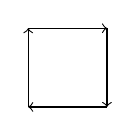
\begin{tikzpicture}
\draw[->] (0,0) -- (0,1);
\draw[->] (0,1) -- (1,1);
\draw[->] (1,1) -- (1,0);
\draw[->] (1,0) -- (0,0);
\end{tikzpicture}
}
in the margin. Note that the only reflective symmetry of the oriented
square is reflection in the center -- and the outcome is the same
as a rotation by $180$\textdegree. However, for $\square$ we would get
reflective symmetries that are not rotations.
It is actually a little difficult to come
up with a simple geometry of the plane that gives exactly the rotational
symmetries of $\square$. Later in the book, we will first pursue an
algebraic approach, using that any rotational symmetry of $\square$
can be reached by doing the $90$\textdegree-rotation a few times, 
together with the fact that taking any loop four times reduces to not doing
anything at all: they represent the \emph{cyclic group of order four}.

A by-product of this line of thinking is the distinguished position of the circle. To express this it is convenient to give names to things: let $\base$ (\ie a dot) be the chosen base point in the circle and $\Sloop$ the loop winding once around the circle counterclockwise. Then a symmetry of a shape $x_0$ in $X$ is uniquely given by the image of $\Sloop $ under a function $\Sc\to X$ taking $\base$ to $x_0$. So,
\begin{quote}
  the study of symmetries is the study of (pointed) functions between types of things, with the circle being the type that gives you access to individual symmetries.
\end{quote}

This is similar to the idea of replacing membership in a set $S$ by function from a one-point set $1$ into $S$: a point $s$ in $S$ is uniquely given by the function $1\to S$ taking the value $s$.


Just as you don't need much information about the one-point set to get this to work, you don't need much information about the circle to embark on a study of symmetries.
Essentially you need to know of $\base $ and $\Sloop $, and that there is no ``hidden relation'' between the symmetries of $\base$. Contrast this to the type of squares which has such a ``hidden relation'': where we identified a $360$\textdegree\ rotation with doing nothing.  This point of view has the benefit of being readily formalized while offering geometric intuition.

\sususe{Symmetries have natural scopes}

The natural scope of the symmetries of a thing $x$ in a type $X$
are the things in $X$ that can be reached from $x$ by a journey in $X$.

Let's make this precise with an example.
In our setup,
as a consequence of univalence, journeys from one set to another
in the type of sets are
uniquely given by one-to-one correspondences between these sets,
commonly called \emph{bijections}.

Now consider the set $\{1,2,3\}$. Then a symmetry of $\{1,2,3\}$ in the type of finite sets amounts to the same thing as a symmetry of $\{1,2,3\}$ in the type of sets with three elements: a symmetry of $\{1,2,3\}$ will not ``pass through'' sets that have, say, five elements. Think of the type of finite sets as being the disjoint union of all the types of sets with $n$-elements, where $n=0,1,2,\dots$: if a symmetry is a loop it should not be allowed to jump between the type of sets with three elements and the type of sets with five elements.\marginnote{%
  Type of empty sets:\\
  \begin{tikzpicture}
    \draw plot [smooth cycle] coordinates {(0,0) (3,-.5) (3.5,1) (1,2)};
    \node[dot,label=above right:{flying elephants}] (fe) at (.5,0) {};
    \node[dot,label=below:{live dodos}] (ld) at (2,1.5) {};
    \node at (1,0.75) {$\cdots$};
  \end{tikzpicture}\\
  Type of one-element sets:\\
  \begin{tikzpicture}
    \draw plot [smooth cycle] coordinates {(0,-.5) (3,0) (3.5,2) (1,1)};
    \node[dot,label=above:{$\{1\}$}] (one) at (1,0) {};
    \node[dot,label=below:{$\{\text{Calvin}\}$}] (calvin) at (2.5,1.3) {};
    \node at (2,0.25) {$\cdots$};
  \end{tikzpicture}\\
  Type of two-element sets:\\
  \begin{tikzpicture}
    \draw plot [smooth cycle] coordinates {(0,1) (1,-1) (3.7,-.5) (3.5,2) (1.5,1.5)};
    \node[dot,label=above:{$\{1,2\}$}] (onetwo) at (.5,.5) {};
    \node[dot,label=below:{$\{\text{Calvin},\text{Hobbes}\}$}]
      (calvinhobbes) at (2.5,1.5) {};
    \node[dot,label=below:{$\{9,\text{Louise}\}$}] (ninelouise) at (3,0.5) {};
    \node[dot,label=above:{$\{\text{Thelma},\text{Hobbes}\}$}]
      (thelmahobbes) at (2,-0.8) {};
    \node at (1.5,0.2) {$\cdots$};
    \node at (1.5,-1.5) {$\vdots$};
  \end{tikzpicture}}

In fact, \emph{any} type $X$ can be naturally divided into ``components'': each
element $x_0$ in $X$ belongs to one and only one component, and the one $x_0$
belongs to we call $\conncomp X {x_0}$, and the symmetries of $x_0$ in $X$ may
be identified with the symmetries of $x_0$ in $\conncomp X {x_0}$. Hence from
the perspective of symmetries of $x_0$ only the component containing it matters,
and we confine our discussion to ``connected'' types of things, \ie those having
just one component.

The geometric intuition also points to the possibility of seemingly different symmetries being identified: when looping once around the circle it shouldn't matter ``how'' or ``how fast'' you do it. Consider the picture of the abelian group on two letters ${\color{casred}a}$ and ${\color{casblue}b}$ from before, but now together with a more frivolous loop (in pink) homotopic to $a$:
\begin{center}
\begin{tikzpicture}
  \useasboundingbox (-3,-1.5) rectangle (3,1.5);
  \begin{scope}[xshift=2.4cm,yshift=.35cm,xscale=cos(25)]
  \draw[casred!25] (0,0) arc (65:425:0.685);
  \draw[casred,line cap=round] (0,0) arc (65:148:0.685);
  \draw[casred] (0,0) arc (65:-55:0.685);
  \end{scope}
  \draw[orange] (2.4,0.35) .. controls ++(.1,-.5) and ++(.6,.3) .. (2,-1.12);
  \draw[orange!25] (2,-1.12) .. controls ++(-.6,-.3) and ++(-.5,-.2) .. (1.21,-0.09);
  \draw[orange] (1.21,-0.09) .. controls ++(.5,.2) and ++(-.2,-.2) .. (2.4,0.35);
  \draw[casblue] (0,.35) ellipse (2.4 and 0.9);
  \draw (0,0) ellipse (3 and 1.5);
  \begin{scope}
    \clip (0,-1.8) ellipse (3 and 2.5);
    \draw (0,2.2) ellipse (3 and 2.5);
  \end{scope}
  \begin{scope}
    \clip (0,2.2) ellipse (3 and 2.5);
    \draw (0,-2.2) ellipse (3 and 2.5);
  \end{scope}
  \node[dot] at (2.4,0.35) {};
  \node (a) at (2.6,-.2) {$a$};
  \node (b) at (0,1) {$b$};
\end{tikzpicture}
\end{center}
You might think of a symmetries of $x_0$ as a rubber band confined to the circle
and pinned to $x_0$. In the picture we've drawn such a rubber band (in orange)
which can be deformed to $a$, and this deformation we consider as
an \emph{identification of the two symmetries}.  In the language we adopt, this
is hard-wired, and so our arguments are independent of any picture: pictures
serve only as inspirations and are very helpful when trying to discover
proofs.\footnote{There's a subtle point, which may be a source of
  confusion if brushed under the carpet: a priori there could be ``several
  ways'' in which two symmetries should be identified. For many purposes this
  poses no problem, but we want to present a theory that mirrors the classical
  theory faithfully, and so restrict our ``types of things'' where there aren't
  multiple ways of identifying symmetries. The technical term -- when we get
  that far will be ``pointed connected groupoids''. This means disallowing types
  like the sphere:
  \begin{center}
    \begin{tikzpicture}
      \draw (0,0) circle (1);
      \draw[casred] (0,0) ellipse (1 and .3);
      \node[dot,label=right:$x_0$] at (1,0) {};
    \end{tikzpicture}
  \end{center}
  There are fundamentally different ways of identifying the symmetry represented
  of $x_0$ by the equator with the trivial symmetry: when thought of as a rubber
  band the equator can contract either over the north or the south poles (or
  more complicated ways). There's something called ``truncation'' which can fix
  any type to one of the desired sort where identifications of symmetries are
  unique.}%endfootnote

Our use of univalent foundations has several advantages. Roughly, univalence is the assertion that two types are ``equivalent'' if and only if there is a ``path'' (called an ``identification'') between them in the (large) ``type of types''. In group theory, two groups share exactly the same properties if there is an ``isomorphism'' between them (an invertible homomorphism), and with univalent foundation this is manifested by the isomorphism corresponding to a path between the groups in the type of groups. Hence we can use this path to transport any theorem about one group to the other: the two groups are ``identified''. The power of univalence is hard to overstate; it will simplify many proofs and make many statements accessible that otherwise would have been out of reach.

There are many kinds of symmetry and many ways of studying it.
Euclidean plane geometry is the study of properties that are invariant under rigid motions of the plane.
Other kinds of geometry arise by considering other notions of transformation.
Univalent mathematics gives a new perspective on symmetries:
Motions of the plane are forms of identifying the plane with itself in possibly non-trivial ways.
It may also be useful to consider different presentations of planes
(for instance as embedded in a common three-dimensional space)
and different identifications between them.
For instance, when drawing images in perspective
we identify planes in the scene with the image plane,
not in a rigid Euclidean way, but
rather via a perspectivity (see~\cref{fig:perspectivity}).
This gives rise to projective geometry.
\begin{marginfigure}
  \begin{center}
    \footnotesize
    \begin{tikzpicture}
      \node[dot,label=left:$O$] (O) at (0,0) {};
      \node[dot,casred,label=below:$A$] (A) at (1,-.3) {};
      \node[dot,casblue,label=below:$A'$] (Ap) at (2,-.6) {};
      \node[dot,casred,label={[label distance=-1pt]-95:$B$}] (B) at (.8,.2) {};
      \node[dot,casblue,label=right:$B'$] (Bp) at (2.4,.6) {};
      \node[dot,casred,label=above:$C$] (C) at (1.05,.7) {};
      \node[dot,casblue,label=above:$C'$] (Cp) at (2.1,1.4) {};
      \draw[casred,fill=casred!25] (A.center) -- (B.center) -- (C.center) -- cycle;
      \draw[casblue,fill=casblue!25] (Ap.center) -- (Bp.center) -- (Cp.center) -- cycle;
      \draw[dashed] (O) -- (Ap.center);
      \draw[dashed] (O) -- (Bp.center);
      \draw[dashed] (O) -- (Cp.center);
    \end{tikzpicture}
  \end{center}
  \caption{A perspectivity identifies the planes determined by the triangles $ABC$ and $A'B'C'$ in a way that doesn't preserve Euclidean distances or angles.}
  \label{fig:perspectivity}
\end{marginfigure}

Does that mean that a plane from the point of view of Euclidean
geometry is not the same as a plane from the point of view of
projective or affine geometry?
Yes.
These are of different types,
because they have different notions of identification,
and thus they have different properties.

Here we follow Quine's dictum: No entity without identity!
To know a type of objects is to know what it means to identify representatives of the type.
The collection of self-identifications (self-transformations) of a given object form a \emph{group}.

% TODO : Propositions, sets, and $1$-types (groupoids). (Here?)

Group theory emerged from many different directions in the latter half of the 19\th century.
Lagrange initiated the study of the invariants under permutations
of the roots of a polynomial equation $f(x)=0$,
which culminated in the celebrated work of Abel and Galois,
proving the unsolvability of general quintic (and higher degree)
polynomials by radicals.
In number theory, Gauss had made detailed studies of modular arithmetic,
proving for instance that the group of units of
$\ZZ/n\ZZ$ is cyclic precisely when $n$ is $1$, $2$, $4$, $p^k$ or $2p^k$, where $p$ is an odd prime and $k > 0$.
Klein was bringing order to geometry by considering groups of transformation,
while Lie was applying group theory in analysis to the study of differential equations.

Galois was the first to use the word ``group'' in a technical sense,
speaking of collections of permutations closed under composition.
He realized that the existence of a resolvent equation is equivalent
to the existence of a normal subgroup of prime index
in the group of the equation.


REMEMBER: a section on planar tessellations [need help here]


\subsection{Who is this book for?}
\label{sec:who}
At the outset the plan for this book was that it ought to cater for two very groups of readers. If you already have a classical first course in abstract group theory, this text has as its ambition that you should gain a new perspective on the material, \emph{and at the same time} learn about homotopy type theory by seeing it applied to a field you are familiar with. However, at the outset, another audience seemed just as plausible to us: what if you're not well versed in abstract algebra, but open to learning about it from a type theoretic perspective? This might apply to a computer science student with aspirations towards the many applications of algebra.

The first audience may have become our predominant target as the book has progressed, partially because it probably is more sizable than the second since most students have been brain-washed to think only in terms of sets at the time they're ready for this book.

\subsection{Outline of the book}
\label{sec:outline}

% describing the same thing gives a particular forceful setup
%
%(still being developed)..}






OLD

This book is about symmetry and its many manifestations in mathematics.

Groupoids vs groups.
The type of all squares in a euclidean plane form a groupoid.
It is connected,
because between any two there exist identifications between them.
But there is no canonical identification.

When we say ``the symmetry group of the square'',
we can mean two things:
1) the symmetry group of a particular square;
this is indeed a group,
or 2) the connected groupoid of all squares;
this is a ``group up to conjugation''.

Vector spaces. Constructions and fields. Descartes and cartesian geometry.

Klein's EP:
\begin{quote}
  Given a manifold and a transformation group acting on it,
  to investigate those properties of figures on that manifold
  that are invariant under transformations of that group.
\end{quote}
and
\begin{quote}
  Given a manifold, and a transformation group acting on it,
  to study its \emph{invariants}.
\end{quote}
Invariant theory had previously been introduced in algebra
and studied by Clebsch and Gordan.

(Mention continuity, differentiability, analyticity and Hilbert's 5\th problem?)

Any finite automorphism group of the Riemann sphere is conjugate to a
rotation group (automorphism group of the Euclidean sphere).
[Dependency: diagonalizability] (Any complex representation of a
finite group is conjugate to a unitary representation.)

% Groups up to conjugation: $\Gal(\bar\Q/Q)$?

All of mathematics is a tale, not about groups,
but about $\infty$-groupoids.
However, a lot of the action happens already with groups.

\newpage

\section*{Glossary of coercions}

MOVE TO BETTER PLACE
Throughout this book we will use the following coercions to make the text more readable.
\begin{itemize}[noitemsep]
\item If $X$ is the pointed type $(A,a)$, then $x:X$ means $x:A$.
\item On hold, lacking context: If $p$ and $q$ are paths, then $(p,q)$ means $(p,q)^=$.
\item If $e$ is a pair of a function and a proof, we also use $e$ for the function.
\item If $e$ is an equivalence between types $A$ and $B$, we use $\etop e$ for the
identification of $A$ and $B$ induced by univalence.
\item If $p: A= B$ with $A$ and $B$ types, then we use $\ptoe p$ for the canonical
equivalence from $A$ to $B$ (also only as function).
%\item If $G$ is the group $(A,a,p,q)$, then $g:G$ means $g: a=_A a$. %TODO: El
\item If $X$ is $(A,a,\ldots)$ with $a:A$, then $\pt_X$ and even just $\pt$ mean $a$.
\end{itemize}

\bigskip

\section*{How to read this book}

\ldots

\noindent\emph{A word of warning.}\enspace
We include a lot of figures to make it easier to follow the material.
But like all mathematical writing, you'll get the most out of it,
if you maintain a skeptical attitude:
Do the pictures really accurately represent the formal constructions?
Don't just believe us: Think about it!

The same goes for the proofs: When we say that something \emph{clearly} follows,
it should be \emph{clear to you}.
So clear, in fact, that you could go and convince a proof assistant,
should you so desire.

\section*{Acknowledgement}
The authors acknowledge the support of the Centre for Advanced Study (CAS)
at the Norwegian Academy of Science and Letters
in Oslo, Norway, which funded and hosted the research project Homotopy
Type Theory and Univalent Foundations during the academic year 2018/19.



%%% Local Variables:
%%% mode: latex
%%% TeX-master: "book"
%%% End:

  %% this chapter sets up the foundational system, which is Univalent Foundations
\chapter{An introduction to univalent mathematics}
\label{ch:univalent-mathematics}

\section{What is a type?}
\label{sec:what-is-a-type}

In some computer programming languages, all variables are introduced along with a declaration of the type of thing they will refer to.  Knowing
the type of thing a variable refers to allows the computer to determine which expressions in the language are \emph{grammatically well
formed}\footnote{The grammar of a programming language consists of all the language's rules.  A statement or expression in a programming
language is grammatically well formed if it follows all the rules.}, and hence valid.  For example, if $s$ is a
string\footnote{A \emph{string} is a sequence of characters, such as ``qwertyuiop''.} and $x$ is a real number, we may write $1/x$, but we may not write $1/s$.%
\footnote{In a programming language, the well formed expression $1/x$ may produce a run-time error if $x$ happens to have the value $0$.}

To enable the programmer to express such declarations, names are introduced to refer to the various types of things.  For example, the name
$\bool$ may be used to declare that a variable is a Boolean value\footnote{A Boolean value is either \emph{true} or \emph{false}.},
  $\integer$ may refer to 32-bit integers, and $\real$ may refer to 64-bit floating point numbers\footnote{An example of a \emph{floating
point number} is $.625 \times 2^{33}$ -- the \emph{mantissa} $.625$ and the \emph{exponent} $33$ are stored inside the floating point number.
The ``point'', when the number is written in base $2$ notation, is called ``floating'', because its position is easily changed by modifying the exponent.}.

Types occur in mathematics, too, and are used in the same way: all variables are introduced along with a declaration of the type of thing they
will refer to.\index{type} For example, one may say ``consider a real number $x$'', ``consider a natural number $n$'', ``consider a point $P$ of
the plane'', or ``consider a line $L$ of the plane''.  After that introduction, one may say that the \emph{type} of $n$ is \emph{natural number} and
that the \emph{type} of $P$ is \emph{point of the
plane}.  Just as in a computer program, type declarations such as those are used to determine which mathematical statements are grammatically
well formed.  Thus one may write ``$P$ lies on $L$'' or $1/x$, but not ``$L$ lies on $P$'' nor $1/L$.\footnote{In mathematics there are no
``run-time'' errors; rather, it is legitimate to write the expression $1/x$ only if we already know that $x$ is a non-zero real number.}

Often ordinary English writing is good enough for such declarations in mathematics expositions, but, for convenience, mathematicians usually
introduce symbolic names to refer to the various types of things under discussion.  For example, the name $\NN$ is usually used when declaring
that a variable is a natural number, the name $\ZZ$ is usually used when declaring that a variable is an integer, and the name $\RR$ is usually
used when declaring that a variable is a real number.  Ways are also given for constructing new type names from old ones: for example, the name
$\RR\times\RR$ may be used when declaring that a variable is a point of the plane, for it conveys the information that a point of the plane is a
pair of real numbers.

Once one becomes accustomed to the use of names such as $\NN$ in mathematical writing and speaking, it is natural to take the next step and
regard those names as denoting things that exist.  Thus, we shall refer to $\NN$ as the \emph{type of all natural numbers}, and we will think of
it as a mathematical object in its own right.  Intuitively and informally, it is a collection whose members (or \emph{elements}) are the natural
numbers.

Once we view the various types as existing as mathematical objects, they become worthy of study.  The language of mathematics is thereby
improved, and the scope of mathematics is broadened.  For example, we can consider statements such as ``$\NN$ is infinite'' and to try to prove
it.

Historically, there was some hesitation\footnote{TO DO : Include some pointers to discussions of potential infinity and actual infinity, perhaps.} about
introducing the collection of all natural numbers as a mathematical object, perhaps because if one were to attempt to build the collection from
nothing by adding numbers to it one at a time, it would take an eternity to complete the assembly.  We won't regard that as an obstacle.

We have said that the types of things are used to determine whether mathematical statements are well formed.
Therefore, if we expect ``$\NN$ is infinite'' to be a well-formed statement, we'll have to know what type of thing $\NN$ is, and we'll
have to have a name for that type.  Similarly, we'll have to know what type of thing that type is, and we'll have to have a name for it,
and so on forever.  Indeed, all of that is part of what will be presented in this chapter.

\section{Types, elements, families, and functions}
\label{univalent-mathematics}

In this section we build on the intuition imparted in the previous section.

In \emph{univalent mathematics},\index{mathematics!univalent}\footnote{The term ``univalent'' is a word coined by Vladimir Voevodsky, who
introduced it to describe his principle that types that are \emph{equivalent} in a certain sense can be identified with each other.  The
principle is stated precisely in \cref{def:univalence}.  As Voevodsky explained, the word comes from a Russian translation of a mathematics
book, where the English mathematical term ``faithful'' was translated into Russian as the Russian word that sounds like ``univalent''.  He also
said ``Indeed these foundations seem to be faithful to the way in which I think about mathematical objects in my head.''} types are used to
classify all mathematical objects.  Every mathematical object is an \emph{element} (or a \emph{member}) of some \emph{type}.  Before
one can talk about an object of a certain type, one must introduce the type itself.  There are enough ways to form new types from old ones to
provide everything we need to write mathematics.

One expresses the declaration that an object $a$ is an element of the \emph{type} $X$ by writing $a:X$.%
\footnote{The notation in mathematics based on \emph{set theory} that corresponds (sort of) to this is $a \in X$.}
\index{element}
\glossary(2:){${:}$}{element judgment}

Using that notation, each variable $x$ is introduced along with a declaration of the form $x:X$, which declares that $x$ will refer to something
of type $X$, but provides no other information about $x$.  The declared types of the variables are used to determine which statements of the
theory are grammatically well formed.

After introducing a variable $x:X$, it may be possible to form an expression $T$ representing a type, all of whose components have
already been given a meaning.
(Here the variable $x$ is regarded also as having already been given a meaning, even though the only thing known about it is its type.)
To clarify the dependence of $T$ on $x$ primarily, we may write $T(x)$ (or $T_x$) instead of $T$.
Such an expression will be called a \emph{family of types} \index{family!of types} parametrized by the variable $x$ of type $X$.
Such a family provides a variety of types, for, if $a$ is any expression denoting an object of $X$, one may replace all
occurrences of $x$ by $a$ in $T$, thereby obtaining a new expression representing a type, which may be regarded as a \emph{member}
and which may be denoted by $T(a)$.

Naturally, if the expression $T$ doesn't actually involve the variable $x$, then the members of the family are all the same,
and we'll refer to the family as a \emph{constant family} of types.

Here's an example of a family of types: let $T$ be the type
of all natural numbers greater than $2$. For any element $n$ of $T$
we let $P_n$ be the type of $n$-sided polygons in the plane.
It gives a family of types parametrized by the elements of $T$.
One of the members of the family is the type $P_5$ of all pentagons in the plane.

A family of types may be parametrized by more than one variable.  For example, after introducing a variable $x:X$ and a family of types $T$
parametrized by $x$, we may introduce a variable $t:T$.  Then it may be possible to form an expression $S$ representing a type that involves the
variables $x$ and $t$.  Such an expression will be called a family of types parametrized by $x$ and $t$, and we may write $S(x,t)$ instead of
$S$ to emphasize the dependence on $x$ and $t$.  The same sort of thing works with more variables.

After introducing a variable $x:X$ and a family of types $T$, it may be possible to form an expression $e$ of type $T$, all of whose components have already been
given a meaning.
Such an expression will also be called a \emph{family of elements of $T$} \index{family!of elements} parametrized by the elements of $X$, when
we wish to focus on the dependence of $e$ (and perhaps $T$) on the variable $x$.
To clarify the dependence of $e$ on $x$ primarily, we may write $e(x)$ (or $e_x$) instead of $e$.
Such a family provides a variety of elements of members of the family $T$, for, if $a$ is any expression denoting an object of $X$, one may replace all
occurrences of $x$ by $a$ in $e$ and in $T$, thereby obtaining an element of $T(a)$, which may be regarded as a \emph{member} of the family $e$
and which will be denoted by $e(a)$.

Naturally, if the expressions $e$ and $T$ don't actually involve the variable $x$, then the members of the family are all the same,
and we'll refer to the family as a \emph{constant family} of elements.

Here's an example of a family of elements in a constant family of types: we let $n$ be a natural number and consider the real number $\sqrt n$.
It gives a family of real numbers parametrized by the natural numbers.
(The family may also be called a \emph{sequence} of real numbers).
One of the members of the family is $\sqrt{11}$.

Here's an example of a family of elements in a (non-constant) family of types.
As above, let $T$ be the type of all natural numbers greater than $2$ and let
$P_n$ be the type of $n$-sided polygons in the plane, for any $n:T$.
Now consider the regular $n$-sided polygon $p_n$ of radius $1$ with
a vertex on the positive $x$-axis, for any $n:T$.  We see that $p_n : P_n$.
One of the members of this family of \emph{elements} $p_n$ is the regular
pentagon $p_5$ of radius $1$ with a vertex on the positive $x$-axis.
The pentagon $p_5$ is an element of the type $P_5$, which is a member of the
family of \emph{types} $P_n$ ($n:T$). In short, $5:T$ and $p_5 : P_5$.

The type $X$ containing the variable for a family of types or a family of elements is called the \emph{parameter type}\index{parameter type} of
the family.

Just as a family of types may depend on more than one variable, a family of elements may also depend on more than one variable.

Families of elements can be enclosed in mathematical objects called \emph{functions}\index{function} (or \emph{maps}\index{map}), as one might
expect.
Let $e$ be a family of elements of a family of types $T$,
both of which are parametrized by the elements $x$ of $X$.  We use the notation $x \mapsto e$ for the function that sends an element $a$ of $X$
to the element $e(a)$ of $T(a)$; the notation $x \mapsto e$ can be read as ``$x$ maps to $e$'' or ``$x$ goes to $e$''.  (Recall that $e(a)$ is
the expression that is obtained from $e$ by replacing all occurrences of $x$ in $e$ by $a$.)  If we name the function $f$, then that element of
$T$ will be denoted by $f(a)$.  The \emph{type} of the function $x \mapsto e$ is called a \emph{product type} and will be denoted by
$\prod_{x:X} T(x)$.\index{product type}\glossary(916Pi){$\prodop_{x:X}T(x)$}{product type of dependent functions}
If $T$ is a constant family of types, then the type will also be
called a \emph{function type} and will be denoted by $X \to T$\glossary(2fun){$\protect\to$}{function type}.  Thus when we write $f : X \to T$,
we mean that $f$ is an element of the type $X \to T$, and we are saying that $f$ is a function from $X$ to $T$.  The type $X$ may be called the
\emph{domain} of $f$, and the type $T$ may be called the \emph{codomain} of $f$.

An example of a function is the function $n \mapsto \sqrt n$ of type $\NN \to \RR$.

Another example of a function is the function $n \mapsto p_n$ of type $\prod_{n:\NN} P_n$, where $P_n$ is the type of polygons introduced above,
and $p_n$ is the polygon introduced above.

Another example of a function is the function $m \mapsto (n \mapsto m+n)$ of type $\NN \to (\NN \to \NN)$.  It is a function that accepts a
natural number as argument and returns a function as its value.  The function returned is of type $\NN \to \NN$.  It accepts a natural number
as argument and returns a natural number as value.

The reader may wonder why the word ``product'' is used when speaking of product types.  To motivate that, we consider a simple example
informally.  We take $X$ to be a type with just two elements, $b$ and $c$.  We take $T(x)$ to be a family of types parametrized by the elements
of $X$, with $T(b)$ being a type with $5$ elements and $T(c)$ being a type with $11$ elements.  Then the various functions $f$ of type
$\prod_{x:X} T(x)$ are plausibly obtained by picking a suitable element for $f(b)$ from the $5$ possibilities in $T(b)$ and by picking a
suitable element for $f(c)$ from the $11$ possibilities in $T(c)$.  The number of ways to make both choices is $5 \times 11$, which is a
\emph{product} of two numbers.  Thus $\prod_{x:X} T(x)$ is sort of like the product of $T(b)$ and $T(c)$, at least as far as counting is
concerned.

The reader may wonder why we bother with functions at all: doesn't the expression $e$ serve just as well as the function $x \mapsto e$, for all
practical purposes?  The answer is no.  One reason is that the expression $e$ doesn't inform the reader that the variable under consideration is
$x$.  Another reason is that we may want to use the variable $x$ for elements of a different type later on: then $e(x)$ is no longer well
formed.  For example, imagine first writing this: ``For a natural number $n$ we consider the real number $\sqrt n$'' and then writing this:
``Now consider a triangle $n$ in the plane.''  The result is that $\sqrt n$ is no longer usable, whereas the function $n \mapsto \sqrt n$ has
enclosed the variable and the family into a single object and remains usable.\footnote{Students of trigonometry are already familiar with the
concept of function, as something enclosed this way.  The sine and cosine functions, $\sin$ and $\cos$, are examples.}

Once a family $e$ has been enclosed in the function $x \mapsto e$, the variable $x$ is referred to as a \emph{dummy variable}\index{dummy
  variable} or as a \emph{bound variable}\index{bound variable}.\footnote{Students of calculus are familiar with the concept of dummy variable
and are accustomed to using identities such as $\int_a^b f(t)\,dt = \int_a^b f(x)\,dx$.} This signifies that the name of the variable no longer
matters, in other words, that $x \mapsto e(x)$ and $t \mapsto e(t)$ may regarded as identical.  Moreover, the variable $x$ that occurs inside
the function $x \mapsto e$ is regarded as unrelated to variables $x$ which may appear elsewhere in the discussion.

If the variable $x$ in our notation $x \mapsto e(x)$ is a dummy variable, and its name doesn't matter, then we may consider the possibility of
not specifying a variable at all.  We introduce now a methodical way to do that, by replacing the occurrences of the variable $x$ in the
expression $e(x)$ by an \emph{underscore},\index{underscore}
yielding $e(\blank)$ as alternative notation for the function $x \mapsto e(x)$.
For example, the
notation $\sqrt{\vphantom{n}\blank}$ can serve as alternative notation for the function $n \mapsto \sqrt n$ introduced above, and $2 + \blank$ can serve as
alternative notation for the function $n \mapsto 2 + n$ of type $\NN \to \NN$.

We have mentioned above the possibility of giving a name to a function.
We expand on that now by introducing notation for making and for using \emph{definitions}.\index{definition}

The notation $x \defeq z$ will be an announcement that we are defining
the expression $x$ to be the expression $z$, all of whose components have already been given a meaning;
in that case, we will say that $x$ has been \emph{defined} to be (or to mean) $z$.%
\glossary(2:=){$\protect\defeq$}{definition}
The forms allowed for the expression $x$ will be made clear by the examples we give.

For example, after writing $n \defeq 12$, we will say that $n$ has
been defined to be $12$.

For another example, naming the function $x \mapsto e(x)$ as $f$
(as we did above) can be done by writing $f \defeq ( x \mapsto e(x) )$.
Alternatively and more traditionally, we may write $f(x) \defeq e(x)$.
Both mean that $f$ has been defined to be $x \mapsto e(x)$
and that, consequently, $f(a)$ has been defined to be $e(a)$,
for any element $a$ of $X$.

The notation $b \jdeq c$ will denote the statement that the expressions $b$ and $c$ become the same thing if all the subexpressions within $b$
or $c$ are expanded according to their definitions, if any; in that case, we will say that $b$ and $c$ are \emph{the same by
definition}\glossary(2==){$\jdeq$}{equality by definition}.  For example, after writing $n \defeq 12$ and $m \defeq n$, we may say that $j + 12
\jdeq j + m$ and that $m \times 11 \jdeq 12 \times 11$.

Whenever two expressions are the same by definition, we may replace one with the other inside any other expression, because the expansion of
definitions is regarded as trivial and transparent.

We proceed now to the promised example.  Consider functions $f : X \to Y$ and $g : Y \to Z$.  We define the \emph{composite} function
$g \circ f : X \to Z$ by setting $g \circ f \defeq (a \mapsto g(f(a)))$.\glossary(2fundef){$\mapsto$}{``maps to'', function definition}\index{composition!of functions}
In other words, it
is the function that sends an arbitrary element $a$ of $X$ to $g(f(a))$ in $Z$.  (The expression $g \circ f$ may be read as ``$g$ circle $f$''
or as ``$g$ composed with $f$''.)  The composite function $g \circ f$ may also be denoted simply by $gf$.\glossary(2circ){$\circ$}{function composition}

Now consider functions $f : X \to Y$, $g : Y \to Z$, and $h : Z \to W$.  Then $(h \circ g) \circ f$ and $h \circ (g \circ f)$ are the same by
definition, since applying the definitions within expands both expressions to $a \mapsto h(g(f(a)))$.  In other
words, we have established that $(h \circ g) \circ f \jdeq h \circ (g \circ f)$.  Thus, we may write $h \circ g \circ f$ for
either expression, without danger of confusion.

One may define the identity function $\id_X : X \to X$ by setting
$\id_X \defeq (a \mapsto a)$.\index{function!identity}
\glossary(id){$\id$}{identity function} Application of definitions shows that
$f \circ \id_X$ is the same by definition as $a \mapsto f(a)$, which, by a standard convention, which we adopt\footnote{The convention that
  $f \jdeq (a \mapsto f(a))$ is referred to as the \emph{$\eta$-rule}\glossary(907-rule){$\eta$}{$\eta$-rule} in the jargon of type theory.}, is to be regarded as the same as $f$.  In
other words, we have established that $f \circ \id_X \jdeq f$.%
\phantomsection\label{page:idofetaf}
A similar computation applies to $\id_Y \circ f$.

In the following sections we will present various other elementary types and elementary ways to make new types from old ones.

\section{Universes}
\label{sec:universes}

In~\cref{univalent-mathematics} we have introduced the objects known as \emph{types}.  They have \emph{elements}, and the type an
element belongs to determines the type of thing that it is.  At various points in the sequel, it will be convenient for types also to be
elements, for that will allow us, for example, to enclose families of types in functions.  To achieve this
convenience, we introduce types that are \emph{universes}.  Some care is required, for the first temptation is to posit a
single new type $\UU$ called \emph{the universe}, so that every type is realized as an element of $\UU$.  This universe would be ``the type of
all types'', but introducing it would lead to an absurdity, for roughly the same reason that introduction of a ``set of all sets'' leads to the absurdity
in traditional mathematics known as Russell's paradox.\footnote{%
  In fact, type theory can trace its origins to Russell's paradox,
  announced in a 1902 letter to Frege as follows:\\
  \begin{adjustwidth}{\parindent}{}
    There is just one point where I have encountered a difficulty.
    You state that a function too, can act as the indeterminate element.
    This I formerly believed,
    but now this view seems doubtful to me because of the following contradiction.
    Let $w$ be the predicate: to be a predicate that cannot be predicated of itself.
    Can $w$ be predicated of itself? From each answer its opposite follows.
    Therefore we must conclude that $w$ is not a predicate.
    Likewise there is no class (as a totality) of those classes which,
    each taken as a totality, do not belong to themselves.
  \end{adjustwidth}
  To which Frege replied:
  \begin{adjustwidth}{\parindent}{}
  Incidentally, it seems to me that the expression
  ``a predicate is predicated of itself'' is not exact.
  A predicate is as a rule a first-level function,
  and this function requires an object as argument
  and cannot have itself as argument (subject).
  \end{adjustwidth}
  Russell then quickly added \emph{Appendex~B} to his
  \emph{Principles of Mathematics} (1903), in which he said that
  ``it is the distinction of logical types that is the key to the whole mystery'',
  where types are the \emph{ranges of significance} of variables.
  For more on the history of type theory,
  see~\citeauthor{sep-type-theory}\footnotemark{}.}\footcitetext{sep-type-theory}
  Some later approaches to set theory included the notion of a \emph{class}, with the collection of all sets being the primary example of a class.
  Classes are much like sets, and every set is a class, but not every class is a set.
  Then one may wonder what sort of thing the collection of all classes would be.  Such
  musings are resolved in univalent mathematics as follows.

\begin{enumerate}
  \item There are some types called \emph{universes}.\index{universe}\glossary(UU){$\protect\UU$}{universe}
  \item If $\UU$ is a universe, and $X : \UU$ is an element of $\UU$, then $X$ is a type.
  \item If $X$ is a type, then it appears as an element in some
  universe $\UU$. Moreover, if $X$ and $Y$ are types,
  then there is a universe $\UU$ containing both of them.
  This universe $\UU$ also contains the type $X\to Y$ and similar
  types constructed from $X$ and $Y$.
  \item\label{it:cumulative} If $\UU$ and $\UU'$ are universes,
  $\UU:\UU'$, $X$ is a type, and $X:\UU$, then also $X:\UU'$.
  (Thus we may regard $\UU'$ as being \emph{larger} than $\UU$.)
  \item There is a particular universe $\UU_0$, which we single out to serve
  as a repository for certain basic types to be introduced in the sequel.
  Moreover, $\UU_0 : \UU$ for every other universe $\UU$,
  and thus $\UU_0$ is the \emph{smallest} universe.
\end{enumerate}

It follows from the properties above that there are an infinite number of
 universes, for each one is an element of a larger one. For the sake of
 clarity, throughout this book, we use an infinite sequence of universes
 $\UU_0 : \UU_1 : \UU_2 : \dots$.

Now suppose we have a type $X$ and a family $T(x)$ of types parametrized by a variable $x$ of type $X$.  Choose a universe $\UU$ with $T(x) : \UU$.
Then we can make a function of type $X \to \UU$, namely $f \defeq (x \mapsto T(x))$.  Conversely, if $f'$ is a function of type $X \to \UU$, then
we can make a family of types parametrized by $x$, namely $T' \defeq f'(x)$.  The flexibility offered by this correspondence between families of
types in $\UU$ and functions to $\UU$ will often be used.

\section{The type of natural numbers}
\label{sec:natural-numbers}

Here are Peano's rules\footcite{peano-principia} for constructing the natural numbers in the form that is used in type theory.
\begin{enumerate}[label=(P\arabic*),ref=(P\arabic*)]
\item\label{P1} there is a type called $\NN$ in the universe $\UU_0$
  (whose elements will be called \emph{natural numbers});%
  \glossary(N){$\protect\NN$}{the type of natural numbers, Peano's rules, \cref{P1}}
\item\label{P2} there is an element of $\NN$ called $0$, called \emph{zero};%
  \glossary(80){$0$}{the natural number zero, Peano's rules, \cref{P2}}\index{zero}
\item\label{P3} if $m$ is a natural number, then there is also a natural number $\Succ(m)$, called the \emph{successor} of $m$;%
  \glossary(succ){$\protect\Succ$}{the successor function on $\NN$, Peano's rules, \cref{P3}}%
  \index{successor}
\item\label{P4} suppose we are given:
  \begin{enumerate}
  \item a family of types $X(m)$ parametrized by a variable $m$ of type $\NN$;
  \item an element $a$ of $X(0)$; and
  \item a family of functions $g_m : X(m) \to X(\Succ(m))$.
  \end{enumerate}
  Then from those data we are provided with a family of elements $f(m) : X(m)$,
  satisfying $f(0) \jdeq a$ and $f(\Succ(m)) \jdeq g_m(f(m))$.
\end{enumerate}

The first three rules present few problems for the reader.  They provide us with the smallest natural number $0:\NN$, and we may introduce as
many others as we like with the following definitions.
\begin{align*}
  1 & \defeq \Succ(0) \glossary(81){$1$}{the natural number 1} \\
  2 & \defeq \Succ(1) \glossary(82){$2$}{the natural number 2} \\
  3 & \defeq \Succ(2) \glossary(83){$3$}{the natural number 3} \\
  & \quad \vdots
\end{align*}

You may recognize rule \ref{P4} as ``the principle of mathematical induction''.\footnote{%
  Rule \ref{P4} and our logical framework are stronger than in Peano's original formulation, and this allows us to omit some rules that Peano had to include:
  that different natural numbers have different successors; and that no number has $0$ as its successor.  Those omitted rules
  remain true in this formulation and can be proved from the other rules, after we have introduced the notion of equality in
  our logical framework.}
We will refer to it simply as ``induction on $\NN$''.

You may also recognize the function $f$ in \ref{P4} as ``defined by recursion''.
The point of the induction principle is that the type $X(m)$ of
$f(m)$ may depend on $m$. An important special case is when $X(m)$
does not depend on $m$, that is, when $X(m)\defeq Y$ for some type Y.
In this non-dependent case we refer to the principle as
``the recursion principle for $\NN$''. In other words, throughout
this book, the difference between an induction principle and the
corresponding recursion principle is that in the latter principle
the type family is constant.
\index{principle!induction}\index{induction principle}
\index{principle!recursion}\index{recursion principle}


The resulting family $f$ may be regarded as having been defined inductively
by the two declarations $f(0) \defeq a$ and $f(\Succ(m)) \defeq g_m(f(m))$,
and indeed, we will often simply write such a pair of declarations as a shorthand way of applying rule \ref{P4}.
The two declarations cover the two ways of introducing elements of $\NN$ via the use of the two rules \ref{P2} and \ref{P3}.
(In terms of computer programming, those two declarations amount to the code for a recursive subroutine that can handle any incoming natural number.)

With that notation in hand, speaking informally, we may regard \ref{P4} above as defining the family $f$ by the following infinite sequence of definitions.
\begin{align*}
  f(0) & \defeq a \\
  f(1) & \defeq g_0(a) \\
  f(2) & \defeq g_1(g_0(a)) \\
  f(3) & \defeq g_2(g_1(g_0(a))) \\
  & \quad \vdots
\end{align*}
(The need for the rule \ref{P4} arises from our inability to write down an infinite sequence of definitions in a finite amount of space, and
from the need for $f(m)$ to be defined when $m$ is a variable of type $\NN$, and thus is not known to be equal to $0$, nor to $1$, nor to $2$,
etc.)

We may use induction on $\NN$ to define of \emph{iteration} of functions.  Let $Y$ be a type, and suppose we have a function $e : Y \to Y$.  We
define by induction on $\NN$ the $m$-fold \emph{iteration} $e^m : Y \to Y$ by setting $e^0 \defeq \id_Y$ and $e^{\Succ(m)}\defeq e\circ e^m$.
(Here we apply rule \ref{P4} with the the type $Y \to Y$ as the family of types $X(m)$, the identity function $\id_Y$ for $a$, and the function
$d \mapsto e\circ d$ for the family $g_m : (Y\to Y)\to(Y\to Y)$ of functions.)

We may now define addition of natural numbers by induction on $\NN$.  For natural numbers $n$ and $m$ we define $n+m : \NN$ by induction on
$\NN$ with respect to the variable $m$ by setting $n+0\defeq n$ and $n+\Succ(m)\defeq \Succ(n+m)$.  (The reader should be able to extract the
family $X(m)$, the element $a$, and the family of functions $g_m$ from that pair of definitions.)  Application of definitions shows, for
example, that $2+2$ and $4$ are the same by definition, and thus we may write $2+2 \jdeq 4$, because both expressions reduce to
$\Succ(\Succ(\Succ(\Succ(0))))$.

Similarly we define the product $m \cdot n : \NN$ by induction on $m$ by setting setting $ 0 \cdot n \defeq 0$ and
$ \Succ(m) \cdot n \defeq (m \cdot n) + n$.

Alternatively (and equivalently) we may use iteration of functions to define addition and multiplication, by setting $n+m \defeq \Succ^m(n)$ and
$m \cdot n \defeq ( i \mapsto i + n )^m (0) $.

Finally, we may define the factorial function%
\index{factorial function}\index{function!factorial}
$\fact : \NN \to \NN$ by induction on $\NN$, setting $\fact(0) \defeq 1$ and
$\fact(\Succ(m)) \defeq \Succ(m) \cdot \fact(m)$.  (One can see that this definition applies rule \ref{P4} with $X(m) \defeq \NN$, with $1$ for
$a$, and with the function $n \mapsto \Succ(m) \cdot n$ for $g_m$.)  Application of the definitions shows, for example, that $\fact(3) \jdeq 6$, as
the reader may verify.

\section{Identity types}
\label{sec:identity-types}

One of the most important types is the \emph{identity type},
which implements a notion of equality.
Identity types are formed of a type and two elements of that type;
we shall have no need to compare elements of different types.

Here are the rules for constructing and using identity types.
\begin{enumerate}[label=(E\arabic*),ref=(E\arabic*)]\label{rules-for-equality}
  \item\label{E1}
    for any type $X$ and for any elements $a$ and $b$ of it, there is an \emph{identity type} $a \eqto b$;%
    \glossary(2=){$\xrightarrow =$}{identity type, \cref{E1}}%
    \index{identity type}
    moreover, if $X$ is an element of a universe $\UU$, then so is $a \eqto b$.
    \marginnote{When the type of $a$ and $b$ is not clear
    we may clarify it by writing $a \eqto_X b$.}
  \item\label{E2} for any type $X$ and for any element $a$ of it, there is an element $\refl a$ of type $a \eqto a$
    (the name $\refl{}$ comes from the word ``reflexivity'')%
    \glossary(refl){$\protect\refl{a}$}{reflexivity, identity type, \cref{E2}}
  \item\label{E3} suppose we are given:
    \begin{enumerate}
    \item a type $X$ and an element $a:X$;
    \item a family of types $P(b,e,\dots)$ parametrized by a variable $b$ of type $X$, a variable $e$ of type $a \eqto b$, and perhaps some
      further variables; and
    \item an element $p$ of $P(a,\refl a,\dots)$.
    \end{enumerate}
    Then from those data we are provided with a family of elements $f(b,e,\dots) : P(b,e,\dots)$.
    Moreover, $f(a,\refl a,\dots) \jdeq p$.
\end{enumerate}

We will refer to an element $i$ of $a \eqto b$ as an
\emph{identification} of $a$ with $b$.
Since the word ``identification'' is a long one,
we may also refer to $i$ as a \emph{path} from $a$ to
$b$ -- this has the advantage of incorporating the intuition that an identification may proceed gradually through intermediate steps.%
\index{identification}

The need to record, using the element $i$, the way we identify $a$
with $b$ may come as a surprise, since normally, in mathematics, one is
accustomed to regarding $a$ as either equal to $b$ or not.
However, this reflects a situation commonly encountered in geometry
when \emph{congruence} of geometric figures is considered.%
\index{congruence}
For example, in Euclidean space, two equilateral triangles of the same size are congruent in six (different)
ways.\footnote{Six, since we allow reflections, otherwise there are only three.\par
  \begin{tikzpicture}[tri/.style={draw,regular polygon,regular polygon sides=3,minimum height=6em}]
    \node[tri,rotate=-15]{};
    \begin{scope}[xshift=7em]
      \node[tri,rotate=15]{};
    \end{scope}
  \end{tikzpicture}
}
The chief novelty of univalent mathematics is that the basic logical notion of equality, as implemented by the identity types $a \eqto b$, is carefully
engineered to accommodate notions of congruence and symmetry from diverse areas of mathematics, including geometry.  Exposing that point of view
in the context of geometry is the main point of this book.

In light of the analogy with geometry just introduced,
we will refer to an element $i$ of $a \eqto a$ as a \emph{symmetry} of $a$.%
\index{symmetry!of an element}
Think, for example, of a congruence of a triangle with itself.
An example of a non-trivial symmetry will be seen in \cref{xca:C2}.

Consider the identity type $\fact(2) \eqto 2$, where $\fact$ denotes the factorial function defined in \cref{sec:natural-numbers}.
Expansion of the definitions in $\fact(2) \eqto 2$ simplifies it to $\Succ(\Succ(0)) \eqto \Succ(\Succ(0))$,
so we see from rule \ref{E2} that $\refl{\Succ(\Succ(0))}$ serves
as an element of it.\footnote{We will see later that numbers only have
trivial symmetries, so the possibility that there are other ways to
identify $\fact(2)$ with $2$ doesn't arise.}
We may also write either $\refl{2}$ or $\refl{\fact(2)}$ for that element.
A student might want a more detailed derivation that $\fact(2)$ may be identified with $2$,
but as a result of our convention above that definitions may be applied without changing anything, the application of definitions, including
inductive definitions, is normally regarded as a trivial operation, and the details are usually omitted.

We will refer to rule \ref{E3} as ``induction for identity''.
To signal that we wish to apply it, we may announce that we argue
\emph{by (path) induction on $e$}, or simply \emph{by path induction}.

The family $f$ resulting from an application of rule \ref{E3} may be regarded as having been completely defined by the single declaration
$f(a,\refl a) \defeq p$,
and indeed, we will often simply write such a declaration as a shorthand way of applying rule \ref{E3}.
The rule says that to construct something from every identification $e$ of $a$ with something else,
it suffices to consider the special case where the identification $e$ is $\refl a : a \eqto a$.%
\footnote{Notice that the single special case in such an induction corresponds to the single way of introducing elements of
identity types via rule \ref{E2}, and compare that with \ref{P4}, which dealt with the two ways of introducing elements of $\NN$.}

Intuitively, the induction principle for identity amounts to saying that the element $\refl a$ ``generates'' the system of types $a \eqto b$, as $b$
ranges over elements of $A$.\footnote{%
  We can also use a geometric intuition: when $b$ ``freely ranges'' over elements of $A$,
  together with a path $e : a \eqto b$,
  while we keep the element $a$ fixed, we can picture $e$ as a piece of string
  winding through $A$, and the ``freeness'' of the pair $(b,e)$ allows us to pull the string $e$,
  and $b$ with it, until we have the constant path at $a$, $\refl a$.\par
  \begin{tikzpicture}
    \draw plot [smooth cycle] coordinates {(0,0) (1.5,0) (1.3,1) (0,1.5)};
    \node[dot,label=above:$a$] (a) at (0.1,0.1) {};
    \node[dot,label=below:$b$] (b) at (1.3,0.8) {};
    \node (A1) at (1.5,1.5) {$A$};
    \draw[->] (a) .. controls ++(-20:1) and ++(170:1) .. node[auto] {$e$} (b);
    \node at (1.9,0.6) {$\mapsto$};
    \begin{scope}[xshift=2.5cm]
    \draw plot [smooth cycle] coordinates {(0,0) (1.5,0) (1.3,1) (0,1.5)};
    \node[dot,label=above:$a$] at (0.1,0.1) {};
    \node at (0.5,0.2) {$\refl a$};
    \node (A2) at (1.5,1.5) {$A$};
    \end{scope}
  \end{tikzpicture}
  Conversely, we can imagine $b$ starting at $a$ and $e$ starting out as $\refl a$, and then think of $b$ roaming throughout $A$, pulling
  the string $e$ along with it, until it finds every path from $a$ to some other element.
}

Equality relations are \emph{symmetric}. For identity types
we establish something similar, taking into account that
the notion of equality implemented here keeps track of the way
two things are identified, and there can be multiple ways.
Given a type $X$ and elements $a$ and $b$ of $X$,
we have an identity type $a \eqto b$
of (zero or more) identifications of $a$ with $b$. We also have
an identity type $b \eqto a$ of identifications of $b$ with $a$.
Symmetry now takes the form of a function from
type $a \eqto b$ to type $b \eqto a$, intuitively reversing
any identification of $a$ with $b$
to give an identification of $b$ with $a$.
In order to produce an element of $b \eqto a$ from an element $e$
of $a \eqto b$, for any $b$ and $e$, we argue by induction on $e$.
We let $P(b,e)$ be $b \eqto a$ for any $b$ of type $X$ and for
any $e$ of type $a \eqto b$, for use in rule \ref{E3} above.
Application of rule \ref{E3} reduces us to the case where $b$ is
$a$ and $p$ is $\refl a$, and our task is now to produce an
element of $a \eqto a$; we choose $\refl a$ for it.

Equality relations are also \emph{transitive}. We proceed in a
similar way as for symmetry. For each $a,b,c:X$ and for each
$p:a \eqto b$ and for each $q:b \eqto c$ we want to produce an
element of type $a \eqto c$.  By induction on $q$ we are reduced
to the case where $c$ is $b$ and $q$ is $\refl b$,
and we are to produce an element of $a \eqto b$.
The element $p$ serves the purpose.
%Notice the similarity of this inductive definition with the definition given above
%of the sum $m+n$. HMM ... (left versus right recursion)

Now we state our symmetry result a little more formally.

\begin{definition}\label{def:eq-symm}
  For any type $X$ and for any $a,b:X$, let
  $$\symm_{a,b} : (a \eqto b) \to (b \eqto a)$$
  be the function defined by induction by setting
  $\symm_{a,a}(\refl a) \defeq \refl a$.

  This operation on paths is called \emph{path inverse}, and we may abbreviate $\symm_{a,b}(p)$ as $p^{-1}$.
  \glossary(1-1){$p^{-1}$}{reverse identification, path inverse, \cref{def:eq-symm}}
\end{definition}

Similarly, we formulate transitivity a little more formally, as follows.

\begin{definition}\label{def:eq-trans}
  For any type $X$ and for any $a,b,c:X$, let $$\trans_{a,b,c} : (a \eqto b) \to ((b \eqto c) \to (a \eqto c))$$ be the function defined by induction by setting
  $(\trans_{a,b,b} (p)) (\refl b ) \defeq p$.

  This binary operation is called \emph{path composition} or \emph{path concatenation}\index{composition!of paths}\index{concatenation!of paths},
  and we may abbreviate $(\trans_{a,b,c}(p))(q)$ as either $p \ct q$, or as $q \cdot p$, $qp$, or $q \circ p$.
  \glossary(2conc){$p\protect\ct q, q\cdot p, qp, q\circ p$}{path concatenation or composition}
\end{definition}

The intuition that the path $p$ summarizes a gradual change from $a$ to $b$, and $q$ summarizes a gradual change from $b$ to $c$, leads to the
intuition that $p \ct q$ progresses gradually from $a$ to $c$ by first changing $a$ to $b$ and then changing $b$ to $c$; see
\cref{fig:path-concatenation}.

The notation $q\circ p$ for path composition, with $p$ and $q$ in reverse order,
fits our intution particularly well when the paths are related to functions and the composition of
the paths is related to the composition of the related functions in the same order, as happens, for example, in connection with {\em transport}
(defined below in \cref{def:transport}) in \cref{xca:trp-compose}.

\begin{marginfigure}
%  \centering
  \begin{tikzpicture}
    \node (X) at (0,-1.5) {$X$};
    \draw (0,-1)
    .. controls ++(200:-1) and ++(180:1) .. (2,-2)
    .. controls ++(180:-1) and ++(270:1) .. (4,0)
    .. controls ++(270:-1) and ++(20:2)   .. (2,2)
    .. controls ++(20:-2)   and ++(90:1)  .. (-1,0)
    .. controls ++(90:-1)  and ++(200:1) .. (0,-1);
    \node[dot,label=below:$a$] (a) at (0,0) {};
    \node[dot,label=below:$b$] (b) at (2,-1) {};
    \node[dot,label=above:$c$] (c) at (3,1) {};
    \node (ct) at (1.2,1) {$q\circ p \jdeq p\ct q$};
    \draw[->] (a) .. controls ++(-20:1) and ++(170:1) .. node[auto,swap] {$p$} (b);
    \draw[->] (b) .. controls ++(170:-1) and ++(-70:1) .. node[auto,swap] {$q$} (c);
    \draw[->] (a) .. controls ++(15:1) and ++(210:1) .. (c);
    %\draw (1,0) arc(210:330:.8 and .5);
    %\draw (2.09,-.18) arc(60:120:.8 and .7);
  \end{tikzpicture}
  \caption{Composition (also called concatenation) of paths in $X$}
  \label{fig:path-concatenation}
\end{marginfigure}

The types of $\symm_{a,b}$ and $\trans_{a,b,c}$ express that
$\eqto$ is symmetric and transitive. Another view of
$\symm_{a,b}$ and $\trans_{a,b,c}$ is that they are
operations on identifications, namely reversing an identification
and concatenating two identifications. The results of various
combinations of these operations can often be identified:
we formulate some of these identifications in the following exercise.

\begin{xca}\label{xca:path-groupoid-laws}
  Let $X$ be a type and let $a,b,c,d:X$ be elements.
  \begin{enumerate}
    \item For $p:a \eqto b$, construct an identification of type $p \ct \refl b \eqto p$.
    \item For $p:a \eqto b$, construct an identification of type $\refl a \ct p \eqto p$.
    \item For $p:a \eqto b$, $q:b \eqto c$, and $r:c \eqto d$, construct an identification of type $(p \ct q) \ct r \eqto p \ct (q \ct r)$.
    \item For $p:a \eqto b$, construct an identification of type $p^{-1} \ct p \eqto \refl b$.
    \item For $p:a \eqto b$, construct an identification of type $p \ct p^{-1} \eqto \refl a$.
    \item For $p:a \eqto b$, construct an identification of type $(p^{-1})^{-1} \eqto p$.
    \qedhere
  \end{enumerate}
\end{xca}

Given an element $p:a \eqto a$, we may use concatenation to define powers $p^n : a \eqto a$
by induction on $n:\NN$; we set $p^0\defeq\refl{a}$ and
$p^{n+1}\defeq p\cdot p^n$. Negative powers $p^{-n}$ are defined
as $(p^{-1})^n$.\footnote{We haven't yet assigned a meaning to $-n$,
  but after we introduce the set of integers $\zet$ below in~\cref{def:zet},
  we'll be justified in writing $p^z$ for any $z:\zet$.  See also \cref{exa:nnn}.}

One frequent use of elements of identity types is in \emph{substitution}\index{substitution}, which is
the logical principle that supports our intuition that when $x$ can by identified with $y$, we may replace $x$ by $y$
in mathematical expressions at will.  A wrinkle new to students will likely be that, in our logical framework
where there may be various ways to identify $x$ with $y$, one must specify the identification used in the substitution.
Thus one may prefer to speak of using an identification to \emph{transport} properties and data about $x$ to properties and data about $y$.

Here is a geometric example: if $x$ is a triangle of area $3$ in the plane, and $y$ is congruent to $x$, then $y$ also has area $3$.

Here is another example: if $x$ is a right triangle in the plane, and $y$ is congruent to $x$, then $y$ is also a right triangle, and
the congruence informs us which of the $3$ angles of $y$ is the right angle.

Now we introduce the notion more formally.

\begin{definition}\label{def:transport}
  Let $X$ be a type, and let $T(x)$ be a family of types parametrized by a variable $x:X$ (as discussed in \cref{univalent-mathematics}).
  Suppose $a,b:X$ and $e:a \eqto b$.
  Then we may construct a function of type $T(a) \to T(b)$.
  The function
  \[
  \trp[T]{e} : T(a) \to T(b)
  \]
  is defined by induction setting $\trp[T]{\refl{a}} \defeq \id_{T(a)}$.%
  \glossary(trp){$\protect\trp[T]{e}$}{transport function, \cref{def:transport}}
\end{definition}

The function thus defined may be called
\emph{the transport function in the type family $T$ along the path $e$},
or, less verbosely, \emph{transport}.\footnote{%
  We sometimes picture this schematically as follows:
  We draw $X$ as a (mostly horizontal) line,
  and we draw each type $T(x)$ as a vertical line lying over $x:X$.
  As $x$ moves around in $X$, these lines can change shape,
  and taken all together they form a $2$-dimensional blob lying over $X$.
  The transport functions map points between the vertical lines.\par
  \begin{tikzpicture}
    % Name the coordinates so they are easy to change
    % first: X
    \coordinate (X-left) at (-1,-1);
    \node[dot,label=below:$a$] (X-x) at (0,-1.2) {};
    \node[dot,label=below:$b$] (X-xp) at (1.5,-.9) {};
    \coordinate (X-right) at (2.8,-1);
    \node (X) at (3,-1) {$X$};
    % then: T top and bottom
    \coordinate (T-top-left) at (-1,1.5);
    \coordinate (T-bot-left) at (-1,0.5);
    \coordinate[label=above:$T(a)$] (T-top-x) at (0,1.9);
    \coordinate (T-bot-x) at (0,-.1);
    \coordinate[label=above:$T(b)$] (T-top-xp) at (1.5,2.1);
    \coordinate (T-bot-xp) at (1.5,.2);
    \coordinate (T-top-right) at (2.8,1.3);
    \coordinate (T-bot-right) at (2.8,0.8);
    \draw (T-bot-left) .. controls +(-90:.5) and +(0:-.5) .. (T-bot-x)
    .. controls +(0:.5) and +(-10:-.5) .. (T-bot-xp)
    .. controls +(-10:.5) and +(90:-.5) .. (T-bot-right)
    -- (T-top-right)
    .. controls +(90:.5) and +(0:.5) .. (T-top-xp)
    .. controls +(0:-.5) and +(-10:.4) .. (T-top-x)
    .. controls +(-10:-.4) and +(90:.5) .. (T-top-left)
    -- (T-bot-left);
    \draw[dashed] (T-bot-x) -- (T-top-x);
    \draw[dashed] (T-bot-xp) -- (T-top-xp);
    \draw (X-left) .. controls +(-10:.3) and +(0:-.3) .. (X-x);
    \draw[->] (X-x) .. controls +(0:.3) and +(-10:-.5) ..
      node[anchor=north] {$e$} (X-xp);
    \draw (X-xp) .. controls +(-10:.5) and +(0:-.1) .. (X-right);
    % Now the specifics: a point t and its transport to T(x')
    \node[dot,label=left:$t$] (t) at (0,0.9) {};
    \node[dot,label=right:${\trp[T]e(t)}$] (tp) at (1.5,1.1) {};
    \draw[mapsto] (t) .. controls +(0:.5) and +(0:-.5) .. (tp);
  \end{tikzpicture}}%
\index{transport}
We may also simplify the notation to just $\trp e$.
The transport functions behave as expected: we may construct an identification of type $\trp {e'\circ e} \eqto \trp {e'} \circ \trp {e}$.
In words: transport along the composition $e\circ e'$ can be identified with the composition of the two
transport functions.  This may be proved by induction in the following exercise.

\begin{xca}\label{xca:trp-compose}
  Let $X$ be a type, and let $T(x)$ be a family of types parametrized by a variable $x:X$.
  Suppose we are given elements $a,b,c:X$, $e:a \eqto b$, and $e':b \eqto c$.  Construct an identification of type
  \[
    \trp {e'\circ e} \eqto \trp {e'} \circ \trp {e}.\qedhere
  \]
\end{xca}

Yet another example of good behavior is given in the following exercise.

\begin{xca}\label{xca:trp-nondep}
  Let $X,Y$ be types.
  As discussed in \cref{univalent-mathematics}, we may regard the expression $Y$ as a constant family of types parametrized by a variable $x:X$.
  Produce an identification of type $\trp[Y]{p} \eqto \id_Y$, for any path $p:a \eqto b$.
\end{xca}

In \cref{sec:props-sets-grpds} below we will discuss what it means for a type to have at most one element.
When the types $T(x)$ may have more than one element,
we may regard an element of $T(x)$ as providing additional \emph{structure} on $x$.
In that case, we will refer to the transport function $\trp e : T(a) \to T(b)$ as
\emph{transport of structure} from $a$ to $b$.

Take, for example, $T(x)\defeq (x \eqto x)$.
Then $\trp e$ is of type $(a \eqto a) \to (b \eqto b)$ and transports a
symmetry of $a$ to a symmetry of $b$.

By contrast, when the types
$T(x)$ have at most one element, we may regard an element of $T(x)$
as providing a proof of a property of $x$. In that case, the transport
function $\trp e : T(a) \to T(b)$ provides a way to establish a claim about $b$
from a claim about $a$, so we will refer to it as \emph{substitution}.  In
other words, elements that can be identified have the same properties.

\section{Product types}
\label{sec:product-types}

Functions and product types have been introduced in \cref{univalent-mathematics}, where we have also explained how to create a function by
enclosing a family of elements in one.  In this section we treat functions and product types in more detail.

Recall that if $X$ is a type and $Y(x)$ is a family of types parametrized by a variable $x$ of type $X$, then there is a \emph{product type}\footnote{%
  Also known as a \emph{Pi-type}.}
$\prod_{x:X} Y(x)$ whose elements $f$ are functions that provide elements $f(a)$ of type $Y(a)$, one for each $a:X$.  We will refer to $X$ as the
\emph{parameter type} of the product.%
\index{product type}\index{Pi type}\index{parameter type}
By contrast, if $Y$ happens to be a constant family of types, then
$\prod_{x:X} Y$ will also be denoted by $X \to Y$, and it will also be called a \emph{function type}.

If $X$ and $Y(x)$ are elements of a universe $\UU$, then so is $\prod_{x:X} Y(x)$.

Functions preserve identity, and we will use this frequently later on.  More precisely, functions induce maps on identity types, as the
following definition makes precise.

\begin{definition}\label{def:ap}
For all types $X$, $Y$, functions $f:X\to Y$ and elements $x,x':X$, the function
$$\ap{f,x,x'} : (x \eqto x') \to (f(x) \eqto f(x'))$$ is defined by induction by setting
$\ap{f,x,x}(\refl{x})\defeq\refl{f(x)}$.%
\glossary(ap){$\protect\ap{f}$}{application of $f$ to a path, \cref{def:ap}}
\glossary(ap){$f(p)$}{application of $f$ to the path $p$, \cref{def:ap}}
\end{definition}

The function $\ap{f,x,x'}$, for any elements $x$ and $x'$ of $X$, is called an \emph{application} of $f$ to paths or to identifications,
and this explains the choice of the symbol $\ap{}$ in the notation for it.
It may also be called the function (or map) \emph{induced} by $f$ on identity types.

When $x$ and $x'$ are clear from the context, we may abbreviate $\ap{f,x,x'}$ by writing $\ap{f}$ instead.
For convenience, we may abbreviate it even further, writing $f(p)$ for $\ap f (p)$.

The following lemma shows that $\ap f$ is compatible with composition.

\begin{construction}\label{lem:apcomp}
  Given a function $f:X\to Y$, and elements $x,x',x'':X$, and paths $p : x \eqto x'$ and $p' : x' \eqto x''$,
  we have an identification of type $\ap f (p' \cdot p) \eqto  \ap f (p') \cdot  \ap f (p)$.

  Similarly, we have that $\ap f$ is compatible with path inverse
  in that we have an identification of type
  $\ap f(p^{-1}) \eqto  (\ap f (p))^{-1}$ for all $p : x \eqto x'$.

  Finally, we have an identification of type $\ap \id (p) \eqto p$ for all
  $p : x \eqto x'$.
\end{construction}

\begin{implementation}{lem:apcomp}
  By induction on $p$ and $p'$, one reduces to producing an identification of type
  \[
    \ap f (\refl x \cdot \refl x) \eqto  \ap f ( \refl x ) \cdot  \ap f ( \refl x ).
  \]
  Both $\ap f (\refl x \cdot \refl x)$ and
  $\ap f ( \refl x ) \cdot  \ap f ( \refl x )$
  are equal to $\refl { f(x) }$ by definition,
  so the identification $\refl {\refl { f(x) }}$ has the desired type.

  The other two parts of the construction are also easily done by induction on $p$.
\end{implementation}

\begin{xca}\label{xca:trp-ap}
  Let $X$ be a type and $T(x)$ a family of types parametrized by a variable $x:X$. Furthermore, let $A$ be a type, let $f:A\to X$ be a
  function, let $a$ and $a'$ be elements of $A$, and let $p: a \eqto a'$ be a path.
  Verify that the two functions $\trp[T \circ f]{p}$ and $\trp[T]{\ap{f}(p)}$ are of type $T(f(a)) \to T(f(a'))$.
  Then construct an identification between them, i.e., construct an element of type $\trp[T \circ f]{p} \eqto \trp[T]{\ap{f}(p)}$.
\end{xca}

If two functions $f$ and $g$ of type $\prod_{x:X} Y(x)$ can be identified, then their values can be identified, i.e., for every element $x$ of
$X$, we may produce an identification of type $f(x) \eqto g(x)$, which can be constructed by induction, as follows.

\begin{definition}\label{def:ptw}
  Let $f,g:\prod_{x:X} Y(x)$. Define the function
  \[
    {\ptw}_{f,g}: ( f \eqto g ) \to \left( \prod_{x:X} f(x) \eqto g(x) \right),
  \]
  by induction by setting ${\ptw}_{f,f}(\refl{f}) \defeq x \mapsto \refl{f(x)}$.
  \footnote{The notation $\ptw$ is chosen to remind the reader of the word ``point-wise'', because the identifications are provided just for each
  point $x$.   An alternative approach goes by considering, for any $x:X$, the evaluation function $\ev_x : \big(\prod_{x:X} Y(x)\bigr) \to Y(x)$ defined by
    $\ev_x(f) \defeq f(x)$.  Then one could define ${\ptw}_{f,g}(p,x) \defeq \ap{\ev_x}(p)$.  The functions provided by these two definitions
  are not equal by definition, but they can be identified, and one can easily be used in place of the other.}
\end{definition}

Conversely, given $f,g:\prod_{x:X} Y(x)$,
from a basic axiom called \emph{function extensionality},%
\index{function extensionality}
postulated below in \cref{def:funext}, an identification $f \eqto g$
can be produced from a family of identifications of type $f(x) \eqto g(x)$
parametrized by a variable $x$ of type $X$.

\begin{definition}\label{def:naturality-square}
Let $X,Y$ be types and $f,g: X\to Y$ functions.
Given an element $h$ of type $\prod_{x:X} f(x) \eqto g(x)$, elements $x$ and $x'$ of $X$, and a path $p: x \eqto x'$,
we have two elements $h(x')\cdot \ap{f}(p)$ and $\ap{g}(p)\cdot h(x)$ of type $f(x) \eqto g(x')$.
We construct an identification
\[
  \ns(h,p): \left(h(x')\cdot \ap{f}(p) \eqto \ap{g}(p)\cdot h(x)\right),
\]
between them by induction, by setting $\ns(h,\refl{x})$ to be some
element of $h(x) \cdot \refl{f(x)} \eqto h(x)$, which can be constructed by induction, as in Exercise \ref{xca:path-groupoid-laws}.%
\glossary(ns){$\protect\ns$}{naturality square, \cref{def:naturality-square}}
The type of $\ns(h,p)$ can be depicted as a square\footnote{%
  \begin{displaymath}
    \begin{tikzcd}[column sep=large,row sep=large,ampersand replacement=\&]
      f(x) \ar[r,"="',"\ap f(p)"] \ar[d,"=","h(x)"'] \& f(x') \ar[d,"="',"h(x')"] \\
      g(x) \ar[r,"=","\ap g(p)"']                    \& g(x')
    \end{tikzcd}
  \end{displaymath}%
} and $\ns(h,p)$ is called a \emph{naturality square}.%
\index{naturality square}
%\footnote{This terminology comes from category theory.}
\end{definition}

\section{Identifying elements in members of families of types}

If $Y(x)$ is a family of types parametrized by a variable $x$ of type $X$, and $a$ and $a'$ are elements of type $X$, then after identifying $a$
with $a'$ it turns out that it is possible to ``identify'' an element of $Y(a)$ with an element of $Y(a')$, in a certain sense.  That is the
idea of the following definition.

\begin{definition}\label{def:pathsoverpaths}
  Suppose we are given a type $X$ in a universe $\UU$ and a family of 
  types $Y(x)$, also in $\UU$, parametrized by a variable $x$ of type $X$.
  Given elements $a,a':X$, $y:Y(a)$, and
  $y':Y(a')$ and a path $p : a \eqto a'$,
  we define a new type $\pathover y Y p {y'}$ in $\UU$ as follows.%
  \glossary(2=over){$\protect\pathover y Y p {y'}$}{path-over type,
    \cref{def:pathsoverpaths}}
  We proceed by induction on $a'$ and $p$, which reduces us to the case where $a'$ is $a$ and $p$ is $\refl a$,
  rendering $y$ and $y'$ of the same type $Y(a)$ in $\UU$, allowing us to define
  $\pathover y Y {\refl a} {y'}$ to be $y \eqto y'$, which is also in $\UU$.
\end{definition}

An element $q : \pathover y Y p {y'}$ is called an \emph{identification} of $y$ with $y'$ \emph{over} $p$, or a
\emph{path} from $y$ to $y'$ \emph{over} $p$.\index{path over}
Intuitively, we regard $p$ as specifying a way for $a$ to change gradually into $a'$, and this provides a way
for $Y(a)$ to change gradually into $Y(a')$; then $q$ charts a way for $y$ to change gradually into $y'$ as $Y(a)$ changes gradually into $Y(a')$.\footnote{\label{ft:path-over-pic}%
  We picture this as follows: the path from $y$ to $y'$ over $p$ travels
  through the vertical lines representing the types $Y(x)$ as $x:X$
  moves along the path $p$ in $X$ from $a$ to $a'$:\par
\begin{tikzpicture}
  % Name the coordinates so they are easy to change
  % first: X
  \coordinate (X-left) at (-1,-1);
  \node[dot,label=below:$a$] (X-x) at (0,-1.2) {};
  \node[dot,label=below:$a'$] (X-xp) at (1.5,-.9) {};
  \coordinate (X-right) at (2.8,-1);
  \node (X) at (3,-1) {$X$};
  % then: Y top and bottom
  \coordinate (Y-top-left) at (-1,1.5);
  \coordinate (Y-bot-left) at (-1,0.5);
  \coordinate[label=above:$Y(a)$] (Y-top-x) at (0,1.9);
  \coordinate (Y-bot-x) at (0,-.1);
  \coordinate[label=above:$Y(a')$] (Y-top-xp) at (1.5,2.1);
  \coordinate (Y-bot-xp) at (1.5,.2);
  \coordinate (Y-top-right) at (2.8,1.3);
  \coordinate (Y-bot-right) at (2.8,0.8);
  \draw (Y-bot-left) .. controls +(-90:.5) and +(0:-.5) .. (Y-bot-x)
  .. controls +(0:.5) and +(-10:-.5) .. (Y-bot-xp)
  .. controls +(-10:.5) and +(90:-.5) .. (Y-bot-right)
  -- (Y-top-right)
  .. controls +(90:.5) and +(0:.5) .. (Y-top-xp)
  .. controls +(0:-.5) and +(-10:.4) .. (Y-top-x)
  .. controls +(-10:-.4) and +(90:.5) .. (Y-top-left)
  -- (Y-bot-left);
  \draw[dashed] (Y-bot-x) -- (Y-top-x);
  \draw[dashed] (Y-bot-xp) -- (Y-top-xp);
  \draw (X-left) .. controls +(-10:.3) and +(0:-.3) .. (X-x);
  \draw[->] (X-x) .. controls +(0:.3) and +(-10:-.5) ..
    node[anchor=north] {$p$} (X-xp);
  \draw (X-xp) .. controls +(-10:.5) and +(0:-.1) .. (X-right);
  % Now the specifics: two points y,y' and the pathover
  \node[dot,label=left:$y$] (y) at (0,0.9) {};
  \node[dot,label=right:$y'$] (yp) at (1.5,1.1) {};
  \draw[->] (y) .. controls +(0:.5) and +(0:-.5) ..
    node[anchor=south] {$q$} (yp);
  \end{tikzpicture}}%

\begin{remark} 
Given a type $Z$, \cref{def:pathsoverpaths} has a special case
in which $Y(x)\defeq Z$ for all $x:X$.
Given elements $a,a':X$, a path $p : a \eqto a'$ and elements $z,z':Z$, 
we can form both the type $\pathover z Y p {z'}$ and the identity 
type $z\eqto z'$. These types are readily identified by induction on $p$.
\end{remark}


The following definition identifies the type of paths over $p$ with a type
of paths using transport along $p$.

\begin{definition}\label{def:pathover-trp}
In the context of \cref{def:pathsoverpaths}, define by induction on $p$ an
identification
$\po_p: \left(\pathover y Y p {y'}\right) \eqto \left( \trp[Y]{p}(y) \eqto y'\right)$ in $\UU$,
by setting $\po_{\refl{x}} \defeq \refl{y \eqto y'}$.%
\glossary(po){$\protect\po_p$}{convert path over path, \cref{def:pathover-trp}}
\end{definition}

Many of the operations on paths have counterparts for paths over paths.
For example, we may define composition of paths over paths as follows.

\begin{definition}\label{def:pathovercomposition}
  Suppose we are given a type $X$ and a family of types $Y(x)$ parametrized by the elements $x$ of $X$.
  Suppose also that we have elements $x, x', x'' : X$, a path $p : x \eqto x'$, and a path $p' : x' \eqto x''$.
  Suppose further that we have elements $y : Y(x)$, $y' : Y(x')$, and $y'' : Y(x'')$, with paths $q : \pathover y Y p {y'}$ over $p$
  and $q' : \pathover {y'} Y {p'} {y''}$ over $p'$.
  Then we define the \emph{composite} path $(q' \pathovercomp q) : \pathover y Y {p' \circ p} {y''}$ over $p' \circ p$ as follows.
  First we apply path induction on $p'$ to reduce to the case where $x''$ is $x'$ and $p'$ is $\refl{x'}$.
  That also reduces the type $\pathover {y'} Y {p'} {y''}$ to the identity type $y' \eqto y''$, so we may apply path induction on $q'$ to reduce
  to the case where $y''$ is $y'$ and $q'$ is $\refl{y'}$.
  Now observe that $p' \circ p$ is $p$, so $q$ provides the element we need.
\end{definition}

Similarly, one can define the inverse of a path over a path,
writing $\inv q : \pathover {y'} Y {\inv p} y$ for the inverse
of $q : \pathover y Y p {y'}$.
For these operations on paths over paths we have identifications
analogous to those for the operations on paths in
\cref{xca:path-groupoid-laws}, after some modification.
For example,
${\inv g} \pathovercomp q$ of type $\pathover {y} Y {{\inv p}\circ p} y$ and
$\refl{y}$ of type $\pathover {y} Y {\refl{x}} y$ cannot be directly used
to form an identity type, since their types are not equal by definition.
We will state these identifications when we need them.

\begin{xca}\label{xca:cp}
Try to state some of these identifications yourself.
\end{xca}

The following construction shows how to handle application of a dependent
function $f$ to paths using the definition above.

\begin{definition}\label{def:apd}
  Suppose we are given a type $X$, a family of types $Y(x)$ parametrized by the elements $x$ of $X$, and a function $f:\prod_x Y(x)$.
  Given elements $x,x':X$ and a path $p : x \eqto x'$, we define
  \[
    \apd{f}(p) : \pathover {f(x)} Y p {f(x')}
  \]
  by induction on $p$, setting
  \[
    \apd f {(\refl x)} \defeq \refl {f(x)}.\qedhere
    \]
    \glossary(apd){$\protect \apd f$}{application of a dependent function
    to a path, \cref{def:apd}}
    \glossary(apd){$f(p)$}{application of dependent $f$ to the path $p$ \cref{def:apd}}
\end{definition}

The function $\apd f$ is called \emph{dependent application} of $f$ to paths.\footnote{%
  We picture $f$ via its \emph{graph} of the values $f(x)$
  as $x$ varies in $X$.
  The dependent application of $f$ to $p$ is then the piece of the graph
  that lies over $p$:\par
  \begin{tikzpicture}
    % Name the coordinates so they are easy to change
    % first: X
    \coordinate (X-left) at (-1,-1);
    \node[dot,label=below:$x$] (X-x) at (0,-1.2) {};
    \node[dot,label=below:$x'$] (X-xp) at (1.5,-.9) {};
    \coordinate (X-right) at (2.8,-1);
    \node (X) at (3,-1) {$X$};
    % then: Y top and bottom
    \coordinate (Y-top-left) at (-1,1.5);
    \coordinate (Y-bot-left) at (-1,0.5);
    \coordinate[label=above:$Y(x)$] (Y-top-x) at (0,1.9);
    \coordinate (Y-bot-x) at (0,-.1);
    \coordinate[label=above:$Y(x')$] (Y-top-xp) at (1.5,2.1);
    \coordinate (Y-bot-xp) at (1.5,.2);
    \coordinate (Y-top-right) at (2.8,1.3);
    \coordinate (Y-bot-right) at (2.8,0.8);
    \draw (Y-bot-left) .. controls +(-90:.5) and +(0:-.5) .. (Y-bot-x)
    .. controls +(0:.5) and +(-10:-.5) .. (Y-bot-xp)
    .. controls +(-10:.5) and +(90:-.5) .. (Y-bot-right)
    -- (Y-top-right)
    .. controls +(90:.5) and +(0:.5) .. (Y-top-xp)
    .. controls +(0:-.5) and +(-10:.4) .. (Y-top-x)
    .. controls +(-10:-.4) and +(90:.5) .. (Y-top-left)
    -- (Y-bot-left);
    \draw[dashed] (Y-bot-x) -- (Y-top-x);
    \draw[dashed] (Y-bot-xp) -- (Y-top-xp);
    \draw (X-left) .. controls +(-10:.3) and +(0:-.3) .. (X-x);
    \draw[->] (X-x) .. controls +(0:.3) and +(-10:-.5) ..
      node[anchor=north] {$p$} (X-xp);
    \draw (X-xp) .. controls +(-10:.5) and +(0:-.1) .. (X-right);
    % Now the specifics: two points y,y' and the pathover
    \coordinate (y-left) at (-1,1.2);
    \node[dot,label=below left:$f(x)$] (y) at (0,0.9) {};
    \node[dot,label=below right:$f(x')$] (yp) at (1.5,1.1) {};
    \coordinate (y-right) at (2.8,1);
    \draw[dotted] (y-left) .. controls +(-10:.3) and +(0:-.5) .. (y);
    \draw[->] (y) .. controls +(0:.5) and +(0:-.5) ..
      node[anchor=south] {$\apd f(p)$} (yp);
    \draw[dotted] (yp) .. controls +(0:.5) and +(120:.1) .. (y-right);
  \end{tikzpicture}}
For convenience, we may abbreviate $\apd f (p)$ to $f(p)$,
when there is no risk of confusion.

The following construction shows how functions of two variables may be applied to paths over paths.

\begin{definition}\label{def:applfun2}
  Suppose we are given a type $X$, a family of types $Y(x)$ parametrized by the elements $x$ of $X$, and a type $Z$.
  Suppose also we are given a function $g : \prod_{x:X} (Y(x) \to Z)$ of two variables.
  Given elements $x,x':X$, $y:Y(x)$, and
  $y':Y(x')$, a path $p : x \eqto x'$, and a path $q :\pathover y Y p {y'}$ over $p$,
  we may construct a path
  \[
    \apap g p q : g(x)(y) \eqto g(x')(y')
  \]
  by induction on $p$ and $q$, setting
  \[
    \apap g {\refl x}{\refl y} \defeq \refl {g(x)(y)}.\qedhere
  \]
\end{definition}

The function $p \mapsto q \mapsto \apap g p q$ is called \emph{application} of $g$ to paths over paths.
For convenience, we may abbreviate $\apap g p q$ to $g(p)(q)$.

The following definition will be useful later.

\begin{definition}\label{def:applfun2comp}
  Suppose we are given a type $X$, a family of types $Y(x)$ parametrized by the elements $x$ of $X$, and a type $Z$.  Suppose also we are given
  a function $g : \prod_{x:X} (Y(x) \to Z)$ of two variables.  Given an element $x:X$, elements $y, y':Y(x)$, and an identification $q : y \eqto y'$, then
  we define an identification of type $\apap g {\refl x} q \eqto \ap {g(x)}(q)$, by induction on $q$, thereby reducing to the case where $y'$ is
  $y$ and $q$ is $\refl y$, rendering the two sides of the equation equal, by definition, to $\refl {g(x)(y)}$.
\end{definition}

\section{Sum types}
\label{sec:sum-types}

There are \emph{sums} of types.
By this we mean if $X$ is a type and $Y(x)$ is a family of types parametrized by a variable $x$ of type $X$, then
there will be a type\footnote{%
  Also known as a \emph{Sigma-type}.}
$\sum _{x:X} Y(x)$%
\index{type!sum}\index{sum type}\index{type!Sigma}\index{sigma type}%
\glossary(918Sigma1){$\sumop _{x:X} Y(x)$}{sum type, of dependent pairs $(x,y)$}
whose elements are all pairs $(a,b)$, where $a:X$ and $b:Y(a)$. Since the type of $b$ may depend on $a$ we also call such a pair
a \emph{dependent} pair. We may refer to $X$ as the \emph{parameter
  type} of the sum.\footnote{%
  We may denote $\sum_{x:X}Y(x)$ by $\Tot(Y)$
  and also call it the \emph{total type} of the family $Y(x)$.
  \index{total type}
  \glossary(totaltype){$\protect\Tot(Y)$}{the total type $\protect\sum_{x:X}Y(x)$}
  We can picture it, in the style of the pictures above,
  as the entire blob lying over $X$. (Each $Y(x)$ is a vertical line over $x:X$,
  and a point $y:Y(x)$ becomes a point $(x,y)$ in the blob.)\par
  \begin{tikzpicture}
    % Name the coordinates so they are easy to change
    % first: X
    \coordinate (X-left) at (-1,-1);
    \node[dot,label=below:$x$] (X-x) at (1,-1.2) {};
    \coordinate (X-right) at (2.8,-1);
    \node (X) at (3,-1) {$X$};
    \node (SXY) at (3,2) {${\sum_{x:X}Y(x)}$};
    % then: Y top and bottom
    \coordinate (Y-top-left) at (-1,1.5);
    \coordinate (Y-bot-left) at (-1,0.5);
    \coordinate[label=above:$Y(x)$] (Y-top-x) at (1,1.9);
    \coordinate (Y-bot-x) at (1,-.1);
    \coordinate (Y-top-right) at (2.8,1.3);
    \coordinate (Y-bot-right) at (2.8,0.8);
    \draw (Y-bot-left) .. controls +(-90:.5) and +(0:-.5) .. (Y-bot-x)
    .. controls +(0:.5) and +(90:-.5) .. (Y-bot-right)
    -- (Y-top-right)
    .. controls +(90:.5) and +(-10:.4) .. (Y-top-x)
    .. controls +(-10:-.4) and +(90:.5) .. (Y-top-left)
    -- (Y-bot-left);
    \draw[dotted] (Y-bot-x) -- (Y-top-x);
    \draw (X-left) .. controls +(10:.3) and +(0:-.3) .. (X-x);
    \draw (X-x) .. controls +(0:.3) and +(0:-.1) .. (X-right);
    % Now the specifics: the pair (x,y) and the projection
    \node[dot,label=left:${(x,y)}$] (y) at (1,0.9) {};
    \draw[->,shorten <=.1cm,shorten >=.1cm] (Y-bot-x)
    -- node[anchor=west] {${\fst}$} (X-x);
  \end{tikzpicture}}

If $X$ and $Y(x)$ are elements of a universe $\UU$, then so is $\sum _{x:X} Y(x)$.

Proving something about (or constructing something from) every
element of $\sum _{x:X} Y(x)$ is done by performing the construction on elements of the form $(a,b)$, for every $a:X$ and $b: Y(a)$.
Two important examples of such constructions are:
\begin{enumerate}
\item \emph{first projection},
$\fst:(\sum _{x:X} Y(x)) \to X$,
$\fst(a,b)\defeq a$;
\item\label{it:second-projection} \emph{second projection},
$\snd(a,b): Y(a)$,
$\snd(a,b)\defeq b$.
\end{enumerate}
In \ref{it:second-projection}, the type of $\snd$ is, in full,
$\prod_{z:\sum_{x:X} Y(x)} Y(\fst(z))$.

\begin{remark}
  \label{rem:non-dependent-sums}
  An important special case of sum types is when the type $Y(x)$ does
  not depend on $x:X$. In that case the sum type $\sum _{x:X} Y(x)$
  is denoted as $X\times Y$ and called a \emph{binary product type},
  see \cref{sec:binprod-types}.
\end{remark}

\begin{remark}
  \label{rem:iterated-sums}
  One may consider sums of sums.  For example, suppose $X$ is a type, suppose $Y(x)$ is a family of types parametrized by a variable $x$ of type $X$,
  and suppose $Z(x,y)$ is a family of types parametrized by variables $x:X$ and $y:Y(x)$.  In this case, the \emph{iterated sum}
  $\sum_{x:X} \sum_{y:Y(x)} Z(x,y)$ consists of pairs of the form $(x,(y,z))$.  For simplicity, we introduce the notation
  $(x,y,z) \defeq (x,(y,z))$, and refer to $(x,y,z)$ as a \emph{triple} or as a \emph{$3$-tuple}.\index{triple}
  \marginnote{%
  Another example of an iterated sum is when $Z'(u)$ is a family of types
  parameterized by a variable $u$ of type $\sum_{x:X} Y(x)$.
  Elements of the type $\sum_{u:\sum_{x:X} Y(x)}Z'(u)$ are triples
  $((x,y),z)$. We use the triple-notation also for this case.}

That process can be repeated: suppose $X_1$ is a type, suppose $X_2(x_1)$
is a family of types parametrized by a variable $x_1$ of type $X_1$,
suppose $X_3(x_1,x_2)$ is a family of types parametrized by variables
$x_1:X_1$ and $x_2:X_2(x_1)$, and so on, up to a family
  $X_n(x_1,\dots,x_{n-1})$ of types.  In this case, the \emph{iterated sum}
  $$\sum _{x_1:X_1} \sum_{x_2:X_2(x_1)} \dots \sum_{x_{n-1}:X_{n-1}(x_1,\dots,x_{n-2})} X_n(x_1,\dots,x_{n-1}) $$
  consists of elements of the form
  $(x_1,(x_2,(\dots (x_{n-1},x_n)\dots)))$; each such element is a pair whose second member is a pair, and so on, so we may refer to it as an \emph{iterated pair}.
  For simplicity, we introduce the notation $(x_1,x_2,\dots,x_n)$ for such an iterated pair, and refer to it as an \emph{$n$-tuple}.\index{tuple}
\end{remark}

\section{Equivalences}\label{sec:equivalence}

Using a combination of sum, product, and identity types allows
us to express important notions, as done in the following
definitions.

The property that a type $X$ has ``exactly one element'' may be made precise
by saying that $X$ has an element such that every other element is equal to it.
This property is encoded in the following definition.

\begin{definition}
  \label{def:contractible}
  Given a type $X$, define a type $\iscontr(X)$ by setting
  \[
    \iscontr(X) \defeq \sum_{c:X} \prod_{x:X} (c \eqto x).\qedhere
  \]
\end{definition}

If $ (c,h) : \iscontr(X) $, then $c$ will be called the \emph{center} of the
the \emph{contraction} $h$, and we call the type $X$ \emph{contractible}.

By path composition, one sees that any element $x : X$ can serve as the center of a contraction of a contractible type $X$.

The following lemma gives an important example of a contractible type.

Given a type $X$ and an element $a$ of $X$,
the \emph{singleton type} $\sum_{x:X} (a \eqto x)$
consists of pairs $(x,i)$ with $i: a \eqto x$. The following lemma shows that a singleton type has exactly one element, justifying the name.

\begin{lemma}\label{lem:thepathspaceiscontractible}
For any type $X$ and $a:X$, the singleton type $\sum_{x:X} (a \eqto x)$ is contractible.
\end{lemma}

\begin{proof}
Take as center the pair $(a,\refl{a})$. We have
to produce, for any element $x$ of $X$ and for any identification
$i: a \eqto x$, an identification of type $(a,\refl{a}) \eqto (x,i)$.  This is done by path induction on $i$, which reduces us to producing
an identification of type $(a,\refl{a}) \eqto (a,\refl{a})$; reflexivity provides one, namely $\refl{(a,\refl{a})}$.
\end{proof}

\begin{definition}
\label{def:fiber}
Given a function $f : X \to Y$ and an element $y:Y$,
the \emph{fiber} (or \emph{preimage}) $f^{-1}(y)$
\index{fiber}\index{preimage}
is encoded by defining $$f^{-1}(y) \defeq \sum_{x:X}(y \eqto f(x)).$$
In other words, an element of the fiber $f^{-1}(y)$ is a pair consisting
of an element $x$ of $X$ and an identification of type $y \eqto f(x)$.
\end{definition}

In set theory, a function $f : X \to Y$ is a bijection if and only if
all preimages $f^{-1}(y)$ consist of exactly one element.
We can also express this in type theory, in a definition due
to Voevodsky, for types in general.

\begin{definition}
  \label{def:equivalence}
  A function $f : X \to Y$ is called an \emph{equivalence} if $\inv f(y)$ is contractible for
  all $y:Y$.  The condition is encoded by the type
\[
\isEq(f) \defeq \prod_{y:Y}\iscontr(f^{-1}(y)).\qedhere
\]
\end{definition}

We may say that $X$ and $Y$ are \emph{equivalent} if we
have an equivalence between them.

\begin{definition}
  \label{def:type-of-equivalences}
  We define the type $X \equivto Y$ of equivalences from $X$ to $Y$
  by the following definition.%
  \glossary(2equivto){$\protect\equivto$}{type of equivalences}
  \[
  (X \equivto Y) \defeq \sum_{f:X\to Y} \isEq(f).\qedhere
  \]
\end{definition}

Suppose $f:X \equivto Y$ is an equivalence, and let $t(y): \iscontr(f^{-1}(y))$, for each $y:Y$, be the corresponding witness to contractibility of the fiber.
Using $t$ we can define an inverse function $g : Y \to X$ by setting $g(y)\defeq\fst(\fst(t(y)))$. This can be seen as follows.

By unfolding all the definitions\footnote{%
  Note that $\fst(t(y)) : \inv f(y)$, so $\fst(\fst(t(y))) : X$ with
  $\snd(\fst(t(y))) : y \eqto f(\fst(\fst(t(y)))).$},
  we have an identification of type $f(g(y)) \eqto y$.
Moreover, $(x,\refl{f(x)})$ is an element of the
fiber $f^{-1}(f(x))$, and $t(f(x))$ is a proof
that this fiber is contractible. Hence the center of contraction
$\fst(t(f(x))$ is identified with $(x,\refl{f(x)})$, and so
$g(f(x))\jdeq(\fst(\fst(t(f(x))))) \eqto x$.

We have shown that $f$ and $g$ are inverse functions.
When it won't cause confusion with the notation for the fibers of $f$,
we will write $f^{-1}$ instead of $g$.

For any type $X$, the identity function $\id_X$ is an
equivalence from $X$ to $X$. To see that, observe that for every
element $a$ in $X$,
$\id_X^{-1}(a)$ is a singleton type and hence is contractible.
This observation, combined with the fact that
$\trp[T]{\refl{x}}\jdeq \id_{T(x)}$, gives that
the function $\trp[T]{e}$ from \cref{def:transport}
is an equivalence from $T(x)$ to $T(y)$, for all $e: x \eqto y$.

\begin{xca}\label{xca:equivalence-invers}
Make sure you understand the two applications of $\fst$
in the definition $f^{-1}(y)\defeq\fst(\fst(t(y)))$ above.
Show that $f^{-1}$ is an equivalence from $Y$ to $X$.
Give a function $(X\equivto Y) \to (Y\equivto X)$.
% and show that our function is an equivalence. Too difficult here.
\end{xca}

\begin{xca}\label{xca:equivalence-comp}
Give  a function $(X\equivto Y) \to ((Y\equivto Z) \to (X\equivto Z))$.
\end{xca}

\begin{xca}\label{xca:2-out-of-3}
  Consider types $A$, $B$, and $C$, functions $f:A\to B$, $g:A\to C$ and $h:B\to C$, together with an element $e: hf \eqto g$.  Prove that if two of
  the three functions are equivalences, then so is the third one.
\end{xca}

The following lemma gives an equivalent characterization
of equivalence that is sometimes easy to use.

\begin{construction}\label{lem:weq-iso}
  Let $X,Y$ be types. For each equivalence $f: X\to Y$, we have a function $g: Y\to X$ such that for all $x:X$ we have $g(f(x)) \eqto x$ and for all
  $y:Y$ we have $f(g(y)) \eqto y$. Conversely, if we have such a function $g$, then $f$ is an equivalence.
\end{construction}
\begin{implementation}{lem:weq-iso}
Given an equivalence $f: X\to Y$ we can take $g \defeq f^{-1}$.
For the converse, see Chapter~4 of the HoTT Book,\footcite{hottbook} or \coqident{Foundations.PartA}{isweq_iso}.
\end{implementation}

We put \cref{lem:weq-iso} immediately to good use.

\begin{lemma}\label{lem:contract-away}
Let $X$ be a type with element $a$, and let
$B(x,i)$ be a type for all $x:X$ and $i: a \eqto x$.
Define $f(x,i): B(x,i) \to B(a,\refl{a})$ by induction on $i$,
setting $f(a,\refl{a},b) \defeq b$ for all $b:B(a,\refl{a})$.
Then $f$ defines an equivalence
\[
f~:~ \sum_{x:X} \sum_{i: a \eqto x} B(x,i) \quad \to \quad B(a,\refl{a}).
\]
\end{lemma}
\begin{proof}
We can also define
$g: B(a,\refl{a})\to \sum_{x:X} \sum_{i: a \eqto x} B(x,i)$
mapping $b: B(a,\refl{a})$ to $(a,\refl{a},b)$.
Clearly $f(g(b)) \eqto b$ for all $b:B(a,\refl{a})$.
Moreover, $g(f(x,i,b)) \eqto (x,i,b)$ is clear by induction
on $i$, for all $b:B(x,i)$.
By \cref{lem:weq-iso} it follows that $f$
is an equivalence.
\end{proof}

The above lemma clearly reflects the  contractibility of the
singleton type $\sum_{x:X}(a \eqto x)$.\footnote{%
  In fact, an alternative proof would go as follows:
  \label{ft:Sigma-assoc}
  First, we use \cref{lem:weq-iso} to construct an element of
  $\sum_{x:X}\sum_{y:Y(x)}Z(x,y)
  \equivto \sum_{w : (\sum_{x:X}Y(x))}Z(\fst w,\snd w)$, i.e.,
  the associativity of sum types, where $X$ is a type,
  $Y(x)$ is a family of types depending on $x:X$,
  and $Z(x,y)$ is a family of types depending on $x:X$ and $y:Y(x)$.
  Then, we construct for any contractible type $X$
  and for any family of types $Y(x)$ depending on $x:X$,
  an equivalence between $\sum_{x:X}Y(x)$ and $Y(c)$,
  where $c$ is the center of contraction of $X$.}
For this reason
we call application of this lemma `to contract away'
the prefix $\sum_{x:X} \sum_{i: a \eqto x}$, in order
to obtain a simpler type. It is often applied
in the following simpler form.

\begin{corollary}\label{cor:contract-away}
With conditions as above, but with $B$ not depending on $i$, the same $f$
establishes an equivalence
\[
 \sum_{x:X} ((a \eqto x)\times B(x))~~\equivto~~B(a).
\]
\end{corollary}

In the direction of further generality, we offer the following exercise.

\begin{xca}\label{xca:sum-equiv-base}
  Suppose $X,Y$ are types related by an equivalence $f : X \to Y$.
  Let $B(x)$ be a type parameterized by $x:X$. Construct an 
  equivalence between $\sum_{x:X}B(x)$ and $\sum_{y:Y}B(\inv{f}(y))$.
\end{xca}

The next exercise gives a dual to \cref{cor:contract-away}
that may be dubbed `to substitute away'.

\begin{xca}\label{xca:substitute-away}
Let $X$ be a type with element $a$, and let
$B(x)$ be a type parameterized by $x:X$.
Give an equivalence between $\prod_{x:X} ((a \eqto x)\to B(x))$ and $B(a)$.
\end{xca}

We proceed now to define the notion of fiberwise equivalence.

\begin{definition}\label{def:fiberwise}
Let $X$ be a type, and let $Y(x),Z(x)$ be families of types parametrized
by $x:X$. A map $f$ of type $\prod_{x:X}(Y(x)\to Z(x))$
can be viewed as a family of maps $f(x): Y(x)\to Z(x)$ and is called a
\emph{fiberwise} map. The \emph{totalization} of $f$ is defined by
$\tot(f)(x,y)\defeq (x,f(x)(y))$.
\index{totalization}
\glossary(totalization){$\protect\tot(f)$}{totalization of $\protect f$}
Using the denotation $\Tot(\blank)$ for the total type of
a type family we thus have
\[
  \tot(f) : \Tot(Y) \to \Tot(Z)).\qedhere
\]
\end{definition}

\begin{lemma}\label{lem:fiberwise}
Let conditions be as in \cref{def:fiberwise}.
If $f(x): Y(x) \to Z(x)$ is an equivalence for every $x:X$
(we say that $f$ is a \emph{fiberwise} equivalence),
%in which case we also call the family $f$ an equivalence,
then $\tot(f)$ is an equivalence.
\end{lemma}
\marginnote{We will allow ourselves to drop the ``fiberwise'' and talk simply about maps and equivalences between type families.}
\begin{proof}
If $f(x): Y(x) \to Z(x)$ is an equivalence for all $x$ in $X$,
then the same is true of all $f(x)^{-1}: Z(x) \to Y(x)$.
Then we have the totalization $\tot(x\mapsto f(x)^{-1})$,
which can easily be proved to be an inverse of $\tot(f)$
(see the next exercise). Now apply \cref{lem:weq-iso}.
\end{proof}

\begin{xca}\label{xca:fiberwise}
Complete the details of the proof of \cref{lem:fiberwise}.
\end{xca}

The converse to \cref{lem:fiberwise} also holds.
\begin{lemma}\label{lem:fiberwise-equiv-from-tot}
  Continuing with the setup of \cref{def:fiberwise},
  if $\tot(f)$ is an equivalence, then $f$ is a fiberwise equivalence.
\end{lemma}
For a proof see~Theorem~4.7.7 of the HoTT Book\footcite{hottbook}.

Yet another application of the notion of equivalence is to postulate axioms.

\begin{principle}\label{def:funext}
The axiom of \emph{function extensionality} postulates that the function
$\ptw_{f,g}: (f \eqto g) \to \prod_{x:X} f(x) \eqto g(x)$ in \cref{def:ptw} is an equivalence.
Formally, we postulate the existence of an element $\funext : \isEq(\ptw_{f,g})$.
From that we can construct the corresponding inverse function
\[
\inv{\ptw}_{f,g}: \Bigl(\prod_{x:X} f(x) \eqto g(x)\Bigr) \to (f \eqto g).
\]
Thus two functions whose values can all be identified can themselves be identified.
This supports the intuition that there is nothing more to a function than the values
it sends its arguments to.
\end{principle}

\begin{xca}\label{xca:Xequiv1toX}
  Let $X$ be a type.  Construct an equivalence of type $( \true \to X ) \equivto X $.
\end{xca}

\begin{xca}\label{xca:XequivXtimes1}
  Let $X$ be a type, and regard $\true$ as a constant family of types over $X$.
  Construct an equivalence of type $( \sum_{x:X} \true ) \equivto X $.
\end{xca}

\begin{xca}\label{xca:Sigma-distrib}
  Let $X$ and $Y$ be types, and let $Z(y)$ be a type parameterized by $y:Y$.
  Construct an equivalence of type
  $\bigl(X\times\sum_{y:Y}Z(y)\bigr) \equivto \sum_{y:Y}(X\times Z(y))$.
\end{xca}

\begin{xca}\label{xca:Sigma-comm}
  Let $X$ and $Y$ be types, and let $Z(x,y)$ be a type parameterized by
  $x:X$ and $y:Y$.
  Construct an equivalence of type $\bigl(\sum_{x:X}\sum_{y:Y}Z(x,y)\bigr)
  \equivto \sum_{y:Y}\sum_{x:X}Z(x,y)$.
\end{xca}

\begin{xca}\label{xca:fib-of-comp}
  Let $X$, $Y$ and $Z$ be types. Given functions $f: X\to Y$ and $g: Y\to Z$,
  construct a family of equivalences of type
  $\inv{(gf)}(z) \equivto \sum_{w:\inv{g}(z)}\inv{f}(\fst w)$ parameterized
  by $z:Z$. Hint: use \cref{ft:Sigma-assoc}.
\end{xca}

\begin{xca}\label{xca:AC-in-TT}
  Let $X$ and $Y$ be types, and let $Z(x,y)$ be a type parameterized by
  $x:X$ and $y:Y$.
  Construct an equivalence of type $\bigl(\prod_{x:X}\sum_{y:Y}Z(x,y)\bigr)
  \equivto \sum_{f:X\to Y}\prod_{x:X}Z(x,f(x))$.\footnote{%
    This equivalence is sometimes called the type-theoretic axiom of choice;
    more prosaically, it expresses the distributivity of products ($\Pi$-types)
    over sums ($\Sigma$-types).
    We discuss the real axiom of choice in~\cref{sec:choicefin}.}
\end{xca}

\begin{xca}\label{xca:section-above-f}
  Let $X$ and $Z$ be types, and let $Y(x)$ be a type parameterized by $x:X$.
  For any function $f:Z\to X$, construct an equivalence
  of type $\bigl(\prod_{z:Z}Y(f(z))\bigr)\equivto 
  \sum_{g:Z\to\sum_{x:X}Y(x)}(f\eqto \fst\circ g)$.\footnote{%
  The special case $Z\jdeq X$, $f\jdeq\id_X$ applies to any product type.}
\end{xca}

\begin{xca}\label{xca:Sigma-curry}\index{currying}
  Let $X$ and $Z$ be types, and let $Y(x)$ be a type parameterized by $x:X$.
  Construct an equivalence\footnote{%
  This canonical equivalence is often called ``currying'',
  after Haskell B.~Curry, and will be treated transparently, \ie
  we will pass between $f(x,y)$ and $f(x)(y)$ without denoting it.
  Note that the equivalence goes between
  $(X\times Y)\to Z$ and $X\to(Y\to Z)$ in case $Y(x)$ is constant.
  }
  of type $\bigl((\sum_{x:X}Y(x))\to Z\bigr)\equivto \prod_{x:X}(Y(x)\to Z)$.
\end{xca}

\section{Identifying pairs}\label{sec:pairpaths}

The identity type of two elements of $\sum _{x:X} Y(x)$ is inductively defined in \cref{sec:identity-types}, as for any other type, but
one would like to express the identity type for pairs in terms of identifications in the constituent types.  This would explain better what it means for
two pairs to be identified.  We start with a definition.

\begin{definition}\label{def:pairtopath}
  Suppose we are given a type $X$ and a family of types $Y(x)$ parametrized by the elements $x$ of $X$.\marginnote{%
    We picture paths between pairs much in the same way as
    paths over paths, cf.~\cref{ft:path-over-pic}.
    Just as, to give a pair in the sum type $\sum_{x:X}Y(x)$,
    we need both the point $x$ in the parameter type $X$
    as well as the point $y$ in $Y(x)$,
    to give a path from $(x,y)$ to $(x',y')$,
    we need both a path $p : x \eqto x'$
    as well as a path $q : \pathover y Y p {y'}$ over $p$.
    Here's a similar picture, where we depict the types in the family
    as being $2$-dimensional for a change.
    \begin{tikzpicture}
    % Name the coordinates so they are easy to change
    % first: X
    \coordinate (X-left) at (-1,-1);
    \node[dot,label=below:$x$] (X-x) at (0,-1.2) {};
    \node[dot,label=below:$x'$] (X-xp) at (1.5,-.9) {};
    \coordinate (X-right) at (2.8,-1);
    \node (X) at (3,-1) {$X$};
    \draw (X-left) .. controls +(-10:.3) and +(0:-.3) .. (X-x);
    \draw[->] (X-x) .. controls +(0:.3) and +(-10:-.5) ..
      node[anchor=north] {$p$} (X-xp);
    \draw (X-xp) .. controls +(-10:.5) and +(0:-.1) .. (X-right);
    % cylinder
    \coordinate (Y-top-left) at (-1,2);
    \coordinate (Y-bot-left) at (-1,0);
    \coordinate (Y-top-x) at (0,1.9);
    \coordinate (Y-center-x) at (0,1);
    \coordinate (Y-bot-x) at (0,0.1);
    \coordinate (Y-top-xp) at (1.5,2.1);
    \coordinate (Y-center-xp) at (1.5,1.1);
    \coordinate (Y-bot-xp) at (1.5,0.1);
    \coordinate (Y-top-right) at (2.8,2);
    \coordinate (Y-bot-right) at (2.8,0.2);
    \draw (Y-top-left) arc (90:450:.2 and 1);
    \fill[opacity=0.6,casred] (Y-center-x) ellipse (.18 and .9);
    \fill[opacity=0.6,casblue] (Y-center-xp) ellipse (.2 and 1);
    \draw (Y-top-x) arc (90:-90:.18 and .9);
    \draw[dashed] (Y-top-x) arc (90:270:.18 and .9);
    \draw (Y-top-xp) arc (90:-90:.2 and 1);
    \draw[dashed] (Y-top-xp) arc (90:270:.2 and 1);
    \draw (Y-top-right) arc (90:-90:.18 and .9);
    \draw[dashed] (Y-top-right) arc (90:270:.18 and .9);
    \draw (Y-top-left) .. controls +(-10:.3) and +(0:-.3) ..
      (Y-top-x) .. controls +(0:.3) and +(-10:-.5) ..
      (Y-top-xp) .. controls +(-10:.5) and +(0:-.1) .. (Y-top-right);
    \draw (Y-bot-left) .. controls +(-10:.3) and +(0:-.3) ..
      (Y-bot-x) .. controls +(0:.3) and +(-10:-.5) ..
      (Y-bot-xp) .. controls +(-10:.5) and +(0:-.1) .. (Y-bot-right);
    % Now the specifics: two points y,y' and the pathover
    \begin{scope}[label distance=2pt]
      \node[dot,label=left:$y$] (y) at (0,0.9) {};
      \node[dot,label=right:$y'$] (yp) at (1.5,1.1) {};
    \end{scope}
    \draw[->] (y) .. controls +(0:.5) and +(0:-.5) ..
      node[anchor=south] {$q$} (yp);
    \end{tikzpicture}}
  Consider the function
  \[
    \pair : \prod_{x:X} \Bigl( Y(x) \to \sum _{x':X} Y(x') \Bigr)
  \]
  defined by
  \[
    \pair(x)(y) \defeq (x,y).
  \]
  For any elements $(x,y)$ and $(x',y')$ of $\sum _{x:X} Y(x)$, we define the map
  \[
    \Bigl( \sum_{p:x \eqto x'} \pathover y Y p {y'} \Bigr)
    \to \left ( (x,y) \eqto (x',y') \right )
  \]
  by
  \[
    (p,q) \mapsto \apap {\pair} p q.
  \]
  (Refer to \cref{def:pathsoverpaths} for the meaning of the type $\pathover y Y p {y'}$, and to \cref{def:applfun2} for the definition of $\constant{apap}$.)
  We introduce $\pathpair p q$ as notation for $\apap {\pair} p q$.
\end{definition}

\begin{construction}\label{cor:isEq-pair=}
  In the situation of \cref{def:pairtopath}, if $x'$ is $x$,
  so that we have $( \pathover y Y {\refl x} {y'} ) \jdeq ( y \eqto y' )$,
  then for any $q : y \eqto y'$, we can construct an identification of type:
  \[
    \pathpair {\refl x} q \eqto \ap {\pair (x)} q
  \]
\end{construction}

\begin{implementation}{cor:isEq-pair=}
  By induction on $q$ it suffices to establish an identification
  \[
    \pathpair {\refl x} {\refl y} \eqto \ap {\pair (x)} (\refl y),
  \]
  both sides of which are
  equal to $\refl {(x,y)}$ by definition.
\end{implementation}

The following lemma gives the desired characterization of paths between pairs.

\begin{lemma}\label{lem:isEq-pair=}
  Suppose we are given a type $X$ and a family of types $Y(x)$ parametrized by the elements $x$ of $X$.
  For any elements $(x,y)$ and $(x',y')$ of $\sum _{x:X} Y(x)$,
  the map defined in \cref{def:pairtopath} defined by
  \[
    (p,q) \mapsto \pathpair p q
  \]
  is an equivalence of type
  \[
    \Bigl( \sum_{p:x \eqto x'} \pathover y Y p {y'} \Bigr)
    \equivto \bigl( (x,y) \eqto (x',y') \bigr).
  \]
\end{lemma}

\begin{proof}
  Call the map $\Phi$.
  A map the other way,
  \[
    \Psi : ((x,y) \eqto (x',y')) \to \sum_{p:x \eqto x'} \pathover y Y p {y'},
  \]
  can be defined by induction, by setting
  \[
    \Psi (\refl {(x,y)}) \defeq (\refl x, \refl y).
  \]
  One proves, by induction on paths, the identifications $ \Psi ( \Phi (p,q) ) \eqto (p,q) $ and $ \Phi (\Psi ( r )) \eqto r$, so $\Psi$ and $\Phi$ are inverse functions.
  Applying \cref{lem:weq-iso}, we see that $\Phi$ and $\Psi$ are inverse equivalences, thereby obtaining the desired result.
\end{proof}

We often use $\fst(\pathpair p q) \eqto p$ and $\snd(\pathpair p q) \eqto q$,
which follow by induction on $p$ and $q$ from the definitions of $\ap{}$ and $\pathpair \_ \_$.
Similarly, $r \eqto \pathpair {\fst(r)}{\snd(r)}$ by induction on $r$.

\section{Binary products}
\label{sec:binprod-types}

There is special case of sum types that deserves to be mentioned since
it occurs quite often. Let $X$ and $Y$ be types, and consider the constant
family of types $Y(x)\defeq Y$. In other words, $Y(x)$ is a type that depends
on an element $x$ of $X$ that happens to be $Y$ for any such $x$.
(Recall \cref{xca:trp-nondep}.)
Then we can form the sum type $\sum_{x:X} Y(x)$ as above.
Elements of this sum type are pairs $(x,y)$
with $x$ in $X$ and $y$ in $Y(x)\jdeq Y$.\footnote{%
  These \emph{cartesian} products we illustrate as usual
  by rectangles where one side represents $X$ and the other $Y$.\par
  \begin{tikzpicture}
    % X
    \coordinate (X-left) at (-.5,-1);
    \node[dot,label=below:$x$] (X-x) at (1.2,-1) {};
    \coordinate (X-right) at (2.5,-1);
    \node (X) at (2.9,-1) {$X$};
    \draw (X-left) -- (X-right);
    % Y
    \coordinate (Y-bot) at (3.5,0);
    \node[dot,label=right:$y$] (Y-y) at (3.5,1) {};
    \coordinate (Y-top) at (3.5,2);
    \node (Y) at (3.5,-.4) {$Y$};
    \draw (Y-top) -- (Y-bot);
    % XY
    \node (SXY) at (.4,.5) {${X\times Y}$};
    \coordinate (XY-top-left) at (-.5,2);
    \coordinate (XY-bot-left) at (-.5,0);
    \coordinate (XY-top-x) at (1,2);
    \coordinate (XY-bot-x) at (1,0);
    \coordinate (XY-y-left) at (0,1);
    \coordinate (XY-y-right) at (2.5,1);
    \coordinate (XY-top-right) at (2.5,2);
    \coordinate (XY-bot-right) at (2.5,0);
    \draw (XY-bot-left) -- (XY-bot-right) -- (XY-top-right)
    -- (XY-top-left) --cycle;
    \draw[dashed] (1.2,0) -- (1.2,2);
    \draw[dashed] (-.5,1) -- (2.5,1);
    \node[dot,label=above left:${(x,y)}$] (xy) at (1.2,1) {};
    \draw[->,shorten <=.1cm,shorten >=.1cm] (1.2,0)
    -- node[anchor=east] {${\fst}$} (X-x);
    \draw[->,shorten <=.1cm,shorten >=.1cm] (2.5,1)
    -- node[anchor=south] {${\snd}$} (Y-y);
  \end{tikzpicture}}
In this case the type of $y$
doesn't depend on $x$, and in this special case the sum type is called
the \emph{binary product}, or \emph{cartesian product} of the types $X$ and $Y$,
denoted by $X \times Y$.
\index{type!binary product}\index{type!cartesian product}
\glossary(2times){$\times$}{cartesian product of two types}

At first glance, it might seem odd that a sum is also a product, but exactly the same thing happens with numbers, for the sum $5+5+5$ is also
referred to as the product $3 \times 5$.  Indeed, that's one way to define $3 \times 5$.

Recall that we have seen something similar with the product type $\prod_{x:X} Y(x)$, which we let $X \to Z$ denote in the case where $Y(x)$ is a
constant family of the form $Y(x)\defeq Z$, for some type $Z$.

The type $X \times Y$ inherits the functions $\fst,\snd$ from
$\sum_{x:X} Y(x)$, with the same definitions $\fst(x,y)\defeq x$
and $\snd(x,y)\defeq y$. Their types can now be denoted in a
simpler way as $\fst: (X \times Y)\to X$ and
$\snd: (X \times Y)\to Y$, and they are called as before the
first and the second projection, respectively.

Again, proving something about (or constructing something from) every
element $(a,b)$ of $X \times Y$ is simply done for all $a:X$ and $b:Y$.

There is an equivalence between $(a_1,b_1) \eqto (a_2,b_2)$ and $(a_1 \eqto a_2) \times (b_1 \eqto b_2)$.
This follows from \cref{lem:isEq-pair=} together with \cref{xca:trp-nondep}.

If $f: X \to Y$ and $f': X' \to Y'$, then we let
$f\times f'$ denote the map of type $(X\times X') \to (Y\times Y')$
that sends $(x,x')$ to $(f(x),f'(x'))$.

The following lemma follows from \cref{lem:isEq-pair=}, combined with \cref{def:pathover-trp} and \cref{xca:trp-nondep}.

\begin{lemma}\label{lem:isEq-pair-bin=}
  Suppose we are given type $X$ and $Y$.
  For any elements $(x,y)$ and $(x',y')$ of $X \times Y$,
  the map defined in \cref{def:pairtopath} defined by
  \[
    (p,q) \mapsto \pathpair p q
  \]
  is an equivalence of type
  \[
    ( x\eqto x' ) \times (y\eqto y') \equivto \left( (x,y)\eqto (x',y')\right).
  \]
\end{lemma}

\begin{xca}\label{xca:binary-prod-equiv}
  Let $X,Y$ be types in a universe $\UU$, and consider the type family
  $T(z)$ in $\UU$ depending on $z:\bool$ defined by
  $T(\no)\defeq X$ and $T(\yes) \defeq Y$.
  Show that the function $(\prod_{b:\bool}T(b))\to X\times Y$
  sending $f$ to $(f(\no),f(\yes))$, is an equivalence.
\end{xca}

\begin{xca}\label{xca:binary-prod-comm}
  Let $X$ and $Y$ be types.
  Construct an equivalence of type $(X \times Y) \equivto (Y\times X)$.
\end{xca}

\section{More inductive types}
\label{sec:inductive-types}

There are other examples of types that are conveniently introduced
in the same way as we have seen with the natural numbers and the identity types.
A type
presented in this style shares some common features: there are some ways to create new elements, and there is a way (called \emph{induction}) to
prove something about every element of the type (or family of types).  We will refer to such types as \emph{inductive} types, and we present a
few more of them in this section, including the finite types, and then we present some other constructions for making new types from old ones.
For each of these constructions we explain the identity type for two
elements of the newly constructed type in terms of identity types for
elements of the constituent types.

\subsection{Finite types}
\label{sec:finite-types}
Firstly, there is the \emph{empty} type in the universe $\UU_0$, denoted by $\emptytype$ or by $\false$.%
  \index{empty type}\index{type!empty}%
  \glossary(0empty){$\protect\emptytype$}{the empty type,
      \cref{sec:finite-types}}%
  \glossary(False){$\protect\false$}{the empty type,
      \cref{sec:finite-types}}
It is an inductive type, with no way
to construct elements of it.  The induction principle for $\emptytype$ says that to prove something about (or to construct something from) every
element of $\emptytype$, it suffices to consider no special cases (!).
Hence, every statement about an arbitrary element of $\emptytype$ can be
proven. (This logical principle is traditionally called
\emph{ex falso (sequitur) quodlibet}.\footnote{%
From falsehood, anything follows. Also called the principle of explosion.})
As an example, we may prove that any two elements $x$ and $y$ of
$\emptytype$ are equal (i.e., construct an identification of
type $x\eqto y$) by using induction on $x$. We may even
prove by induction on $x:\emptytype$ that the elements
$0$ and $\Succ(0)$ of $\NN$ are equal
(i.e., construct a function of type $\emptytype\to(0\eqto\Succ(0)$).

An element of $\emptytype$ will be called an \emph{absurdity}.  Of course, one expects that there are no real absurdities in mathematics, nor in any
logical system (such as ours) that attempts to provide a language for mathematics, but it is important to have such a name so we can discuss
the possibility, which might result inadvertently from the introduction of unwarranted assumptions.  For example, to assert that a type $T$ has
no elements, it would be sensible to assert that an element of $T$ would lead to an absurdity.  Providing a function of type $T \to \emptytype$ is a
convenient way to make that assertion.

Secondly, there will also be an inductive type called $\true$ in the universe $\UU_0$ provided with a single element $\triv$; (the name $\triv$
comes from the word ``trivial'').%
  \index{unit type}\index{type!unit}%
  \glossary(true){$\protect\true$}{the unit type,
      \cref{sec:finite-types}}%
  \glossary(triv){$\protect\triv$}{the element of the unit type,
      \cref{sec:finite-types}}
Its induction principle states that, in order to prove something about (or to construct something from) every
element of $\true$, it suffices to consider the special case where the element is $\triv$.  As an example, we may construct, for any element
$u : \true$, an identification of type $u \eqto \triv$; we use induction to reduce to the case where $u$ is $\triv$, and then $\refl{\triv}$ provides the
desired element.  One may also construct, for any elements $x$ and $y$ of $\true$, an identification of type $x \eqto y$ by using induction both on $x$ and
on $y$.

There is a function $X \to \true$, for any type $X$, namely: $a \mapsto \triv$.  This corresponds, for propositions, to the statement that an
implication holds if the conclusion is true.

\begin{xca}\label{xca:True-univ-prop}
  Let $X$ be a type. Define the function $e$ of type
  $(\true\to X) \to X$ by $e(f)\defeq f(\triv)$.
  Prove that $e$ is an equivalence.
  This is called \emph{the universal property of} $\true$.
\end{xca}

Thirdly, there will be an inductive type called $\bool$ in the universe $\UU_0$, provided with two elements, $\yes$ and $\no$.%
  \index{type!of booleans}%
  \glossary(yes){$\protect\yes$}{the affirmative boolean,
      \cref{sec:finite-types}}%
  \glossary(no){$\protect\no$}{the denying boolean,
      \cref{sec:finite-types}}
Its induction
principle states that, in order to prove something about (or to construct something from) every element of $\bool$, it suffices to consider two
cases: the special case where the element is $\yes$ and the special case where the element is $\no$.

We may use substitution to construct an element of type
$(\yes \eqto \no)\to \emptytype$, expressing that the identification
of $\yes$ with $\no$ leads to an absurdity.
To do this, we introduce a family of types $P(b)$ in the universe
$\UU_0$ parametrized by a variable $b:\bool$.  We define $P(b)$ by induction on $b$ by setting $P(\yes) \defeq \true$ and
$P(\no) \defeq \false$.  (The definition of $P(b)$ is motivated by the expectation that we will be able to construct an equivalence between $P(b)$ and
$\yes \eqto b$.)  If there were an element $e: \yes \eqto \no$, we could substitute $\no$ for $\yes$ in $\triv : P (\yes)$ to get an element of $P(\no)$,
which is absurd.  Since $e$ was arbitrary, we have defined a function $(\yes \eqto \no) \to \emptytype$, as desired.

In the same way, we may use substitution to prove that it is absurd
that successors of natural numbers are identical to $0$,
\ie for any $n:\NN$ that $(0 \eqto \Succ(n))\to \emptytype$.
To do this, we introduce a family of types $P(i)$ in $\UU_0$ parametrized
by a variable $i:\NN$.  Define $P$ recursively by
specifying that $P(0) \defeq \true$ and $P(\Succ(m)) \defeq \false$.  (The definition of $P(i)$ is motivated by the expectation that we will be
able to construct an equivalence between $P(i)$ and $0 \eqto i$.)  If there were an element $e: 0 \eqto \Succ(n)$, we could substitute $\Succ(n)$ for $0$
in $\triv : P ( 0 )$ to get an element of $P(\Succ(n))$, which is absurd.  Since $e$ was arbitrary, we have defined a function $(0 \eqto \Succ(n)) \to \emptytype$,
establishing the claim.

In a similar way we will in \cref{sec:typeFin} define types $\bn n$ for any $n$ in $\NN$
such that $\bn n$ is a type (set) of $n$ elements.


\subsection{Binary sums}
\label{sec:binsum-types}
For sum types of the form $\sum_{b:\bool} T(b)$, with $T(b)$
a type depending on $b$ in $\bool$, there is an equivalence with a simpler type.\footnote{%
  In a case like this, we can thicken up the lines denoting
  $T(\no)$ and $T(\yes)$ in our picture, if we like:\par
  \begin{tikzpicture}
    \node[dot,label=below:${\no}$] (no) at (0,-.8) {};
    \node[dot,label=below:${\yes}$] (yes) at (1.5,-.8) {};
    \node (Bool) at (2.5,-.8) {$\bool$};
    \draw (0,0.9) ellipse (.25 and 1);
    \node (Tno) at (0,2.2) {$T(\no)$};
    \draw (1.5,1.1) ellipse (.4 and 0.8);
    \node (Tyes) at (1.5,2.2) {$T(\yes)$};
    \node[dot,label=above:$x$] (x-no) at (0,0.8) {};
    \node[dot,label=below:$y$] (y-yes) at (1.5,1.2) {};
  \end{tikzpicture}}
After all, the type family $T(b)$ is fully determined
by two types, namely by the types $T(\no)$ and $T(\yes)$.
The elements of $\sum_{b:\bool} T(b)$ are dependent pairs $(\no,x)$ with
$x$ in $T(\no)$ and $(\yes,y)$ with $y$ in $T(\yes)$. The resulting
type can be viewed as the \emph{disjoint union} of $T(\no)$ and $T(\yes)$:
from an element of $T(\no)$ or an element of $T(\yes)$
we can produce an element of $\sum_{b:\bool} T(b)$.

These disjoint union types can be described more clearly in the following way.
The \emph{binary sum} of two types $X$ and $Y$, denoted
\index{type!binary sum}\index{binary sum type}%
\glossary(2amalg){$\amalg$}{binary sum}%
\glossary(inl){$\protect\inl{}$}{inclusion of left summand}%
\glossary(inr){$\protect\inr{}$}{inclusion of right summand}%
$X \amalg Y$,
is an inductive type with two constructors: $\inl{} : X \to X \amalg Y$ and
$\inr{} : Y \to X \amalg Y$.\footnote{%
  Beware that in a picture, the same point may refer
  either to $x$ in $X$ or to $\inl x$ in the sum $X \amalg Y$:\par
  \begin{tikzpicture}
    \draw (0,0.9) ellipse (.25 and 1);
    \node (X) at (0,2.1) {$X$};
    \draw (1,1.1) ellipse (.4 and 0.8);
    \node (Y) at (1,2.1) {$Y$};
    \node[dot,label=above:$x$] (x) at (0,0.8) {};
    \node[dot,label=below:$y$] (y) at (1,1.2) {};
    \draw[dashed] (0.5,1.1) ellipse (1.2 and 1.6);
    \node (XY) at (-0.75,2.35) {$X \amalg Y$};
  \end{tikzpicture}}
Proving a property of any element of $X \amalg Y$
means proving that this property holds of any $\inl{x}$ with $x:X$ and any
$\inr{y}$ with $y:Y$. In general, constructing a function $f$ of type
$\prod_{z: X \amalg Y} T(z)$, where $T(z)$ is a type depending on
$z$, is done by defining $f(\inl{x})$ for all $x$ in $X$
and $f(\inr{y})$ for all $y$ in $Y$.

\begin{xca}\label{xca:binary-sum-equiv}
  Let $X,Y$ be types in a universe $\UU$, and consider the type family
  $T(z)$ in $\UU$ depending on $z:\bool$ defined by induction on $z$ by
  $T(\no)\defeq X$ and $T(\yes) \defeq Y$.
  Show that the map $f : X\amalg Y \to \sum_{b:\bool}T(b)$,
  defined by $f (\inl x) \defeq (\no,x)$ and $f(\inr y) \defeq (\yes,y)$,
  is an equivalence.
\end{xca}

Identification of two elements $a$ and $b$ in $X \amalg Y$ is
only possible if they are constructed with the same constructor.
Thus $\inl{x} \eqto \inr{y}$ is always empty, and there are equivalences of type
$(\inl{x} \eqto \inl{x'}) \equivto (x \eqto x')$ and
$(\inr{y} \eqto \inr{y'}) \equivto (y \eqto y')$.

\begin{xca}\label{xca:binary-sum-id}
  Prove these statements using \cref{xca:binary-sum-equiv},
  \cref{lem:isEq-pair=}, and a characterization
  of the identity types of $\bool$.
\end{xca}

\begin{xca}\label{xca:bin-sum-univ-prop}
  Let $X$, $Y$, $Z$ be types. Define a function $e$ from
  $(X\amalg Y)\to Z$ to $(X\to Z)\times(Y\to Z)$ by precomposition
  with the constructors.
  Prove that $e$ is an equivalence.
  This is called \emph{the universal property of the binary sum}.
\end{xca}

\begin{xca}
  Let $X$ be a type.  Construct an equivalence of type $(X \amalg \emptytype) \equivto X$.
\end{xca}

\subsection{Unary sums}\label{sec:unary-sum-types}

Sometimes it is useful to be able to make a copy of a type $X$:
A new type that behaves just like $X$,
though it is not equal to $X$ by definition.
The \emph{unary sum} or \emph{wrapped copy} of $X$ is an inductive type $\Copy(X)$
\index{type!unary sum}\index{unary sum type}\index{wrapped copy type}%
\glossary(inc){$\protect\inc{}$}{inclusion into wrapped copy}%
with a single constructor, $\inc{} : X \to \Copy(X)$.\footnote{%
  A point $x:X$ corresponds to the point $\inc{x}:\Copy(X)$:\par
  \begin{tikzpicture}
    \draw (0,1) ellipse (.3 and .8);
    \draw[dashed] (-.1,1) ellipse (.6 and 1.1);
    \node[dot,label=above:$x$] (x) at (0,0.8) {};
    \node (X) at (-.45,.7) {$X$};
    \node (c) at (.75,1) {$\leftrightarrow$};
    \draw[dashed] (1.7,1) ellipse (.3 and .8);
    \draw (1.6,1) ellipse (.6 and 1.1);
    \node[dot,label=above:$\inc{x}$] (inx) at (1.7,0.8) {};
    \node (Xdashed) at (2.6,.1) {$\Copy(X)$};
  \end{tikzpicture}\par
  \noindent Note that $\Copy(X)$ can alternatively be defined as $\sum_{z:\true}X$.}
Constructing a function $f : \prod_{z:\Copy(X)}T(z)$,
where $T(z)$ is a type depending on $z : \Copy(X)$,
is done by defining $f(\inc{x})$ for all $x:X$.
Taking $T(z)$ to be the constant family at $X$,
we get a function, $\out : \Copy(X) \to X$,
called the \emph{destructor},
with $\out(\inc{x}) \defeq x$ for $x:X$,
and the induction principle implies that $\inc{\out(z)} \eqto z$
for all $z:\Copy(X)$, so there is an equivalence of type
$\Copy(X) \equivto X$, as expected.
It follows that there are equivalences of type
$(\inc{x} \eqto \inc{x'}) \equivto (x \eqto x')$ and
$(\out(z) \eqto \out(z')) \equivto (z \eqto z')$.

Note that we can make several copies of $X$ that are not
equal to each other by definition,
for instance, by picking different names for the constructor.
We write $\Copy_{\constructor{con}}(X)$ for a copy of $X$
whose constructor is
\[
  \constructor{con} : X \to \Copy_{\constructor{con}}(X).
\]

\begin{example}\label{exa:nnn}
Here's an example to illustrate why it can be useful to make such a wrapped type:
We introduced the natural numbers $\NN$ in \cref{sec:natural-numbers}.
Suppose we want a type consisting of negations of natural numbers,
$\set{\ldots, -2, -1,0}$,
perhaps as an intermediate step towards building the set of integers
$\set{\ldots, -2, -1,0,1,2,\ldots}$.\footnote{%
  We implement this in \cref{def:zet}.}
Of course, the type $\NN$ itself would do,
but then we would need to pay extra attention to whether $n:\NN$
is supposed to represent $n$ as an integer or its negation.
So instead we take the wrapped copy $\NNN\defeq\Copy_{-}(\NN)$,
with constructor ${-} : \NN \to \NNN$.%
\glossary(NNN){$\protect\NNN$}{the type of negated natural numbers,
  \cref{exa:nnn}}
We will also write ${-} : \NNN \to \NN$ for the destructor,
inductively defined by $-(-n)\defeq n$. (The ambiguity will
always be resolved by the types.) In fact, the constructor
and the destructor are each other's inverse since we
also have $-(-(-n))\jdeq -n$, and so by induction $-(-m) = m$ for all $m:\NNN$.
By \cref{lem:weq-iso} we get that they are equivalences.
\end{example}

\subsection{Lists}\label{sec:lists}

One other very common inductive type is that of \emph{lists}
over a given type $X$.
Intuitively, a list of elements of type $X$ is a
sequence $x_1x_2\ldots x_n$ of elements of $X$,
which is possibly the \emph{empty list}, denoted $\varepsilon$.
That is, we allow $n=0$.
The number of elements $n$ is called the \emph{length} of the list.

More formally, we have the following:
% definition
\begin{definition}\label{def:lists}
  For any type $X$, let $X^*$ be the type of lists of elements of $X$.\footnote{%
    In other places, the type of lists is denoted $\casop{\typeformer{List}} X$
    or $[X]$.}
  This is the inductive type with constructors $\varepsilon : X^*$
  (\emph{the empty list}) and \emph{concatenation}%
  \index{list type}\index{type!of lists}%
  \glossary(905epsilon){$\varepsilon$}{the empty list, \cref{def:lists}}%
  \glossary(1Tstar){$X^*$}{list of elements of $X$}%
  \footnote{%
    This constructor doesn't have a name for us,
    since all it does is juxtapose its two arguments.
    It is often called ``cons'',
    as it is a kind of prototypical constructor,
    since many other kinds of data can be represented
    in terms of lists. This is the basis of Lisp:
    the \emph{lis}t \emph{p}rocessing programming language.}
  of type $X \to X^* \to X^*$,
  taking an element $x:X$ and a list $\ell$ to the extended list $x\ell$
  consisting of $x$ followed by the elements of $\ell$.
  In the extended list $x\ell$, $x$ is called the \emph{head}
  and $\ell$ is called the \emph{tail}.\index{list!head}\index{list!tail}
\end{definition}

As an inductive type, $X^*$ comes with a induction principle:
Constructing a function $f$ of type $\prod_{\ell:X^*} T(\ell)$,
where $T(\ell)$ is a type depending on $\ell:X^*$,
may be done by giving:
\begin{enumerate}
\item an element $t_\varepsilon : T(\varepsilon)$; and
\item a family of functions $g_{x,\ell} : T(\ell) \to T(x\ell)$.
\end{enumerate}
The resulting function satisfies $f(\varepsilon) \jdeq t_\varepsilon$
and $f(x\ell) \jdeq g_{x,\ell}(f(\ell))$.
That is, we can produce a function on all lists by specifying how
to handle the empty list and how to reduce the case of an
extended list to that of its tail.

For example, we can define a function $\len : X^* \to \NN$,
giving the length of a list,
satisfying $\len(\varepsilon) \jdeq 0$ and $\len(x\ell) \jdeq \Succ(\len(\ell))$.

\begin{xca}\label{xca:list-contr}
  Prove that $\len : X^* \to \NN$ is an equivalence
  whenever $X$ is contractible.
\end{xca}

Note that there are no general functions producing the
head and tail of an arbitrary list, since the empty list
has neither head nor tail.
However, we can use binary sums with the one-element type $\true$
to define
\[
  \hd : X^* \to X \coprod\true, \quad
  \tl : X^* \to X^* \coprod\true
\]
satisfying $\hd(\varepsilon) \jdeq \inr{\triv}$,
$\hd(x\ell) \jdeq \inl{x}$,
$\tl(\varepsilon) \jdeq\inr{\triv}$,
and $\tl(x\ell) \jdeq \inl{\ell}$.

\begin{xca}\label{xca:reverse}
  Define a function of type $X^* \to X^* \to X^*$ that
  concatenates two lists. (Hint: Use induction on the first argument.)

  Use this to define a function $\rev: X^* \to X^*$ that reverses a list.
\end{xca}

\begin{xca}\label{xca:concat-assoc}
  Construct an identification of type
  $\ell_1(\ell_2\ell_3) \eqto (\ell_1\ell_2)\ell_3$
  for any $\ell_1,\ell_2,\ell_3 : X^*$. (Hint: Use induction on $\ell_1$.)
\end{xca}

We shall see in~\cref{thm:isset-inductive-types} below
that $X^*$ is a set whenever $X$ is.
\Cref{xca:concat-assoc} shows that concatenation of lists
is associative, so we don't need to use parentheses to indicate grouping
within a list. It also justifies denoting both the binary constructor and
concatenation as juxtaposition, with no separate symbol or name.

\section{Univalence}\label{sec:univax}

The univalence axiom, to be presented in this section, greatly enhances
our ability to produce identifications between the two types and to use the
resulting identifications to transport (in the sense of \cref{def:transport})
properties and structure between the types.  It asserts that if $\UU$
is a universe, and $X$ and $Y$ are types in $\UU$, then a specific function,
mapping identifications between $X$ and $Y$ to equivalences between
$X$ and $Y$, is an equivalence.

We now define the function that the univalence axiom postulates
to be an equivalence.

\begin{definition}\label{def:idtoeq}
  For types $X$ and $Y$ in a universe $\UU$ and a path $p : X \eqto Y$,
  transport along $p$ in the type family $\id_\UU$ is a function
  from $X$ to $Y$. We recall the definition by path induction
  from \cref{def:transport}, setting $\trp[\id_\UU]{\refl{X}}\defeq\id_X$.
  As observed in \cref{sec:equivalence}, transport functions are
  equivalences, so that the result is a function
  \[
    (p\mapsto \trp[\id_\UU]{p}) : (X \eqto Y) \to (X\equivto Y).
    \qedhere
  \]
\end{definition}
We may write $\trp[\id_\UU]{p}$ more briefly as $\ptoe p$,%
\glossary(1trp){$\protect\ptoe p$}{transport between types along a path}
which we also use to denote the corresponding function of type $X\to Y$,
instead of $X\equivto Y$.

We are ready to state the univalence axiom.

\begin{principle}[Univalence Axiom]\label{def:univalence}
    Let $\UU$ be a universe.
    Voevodsky's \emph{univalence axiom}\index{univalence axiom} for $\UU$
    postulates that $p\mapsto \ptoe p$ is an equivalence
    of type $(X \eqto Y) \to (X\equivto Y)$, for all $X,Y:\UU$.
    Formally, we postulate the existence of a family of elements
    \[
      \ua_{X,Y} : \isEq((p:X\eqto Y)\mapsto \trp[\id_\UU]{p})
    \]
    \glossary(ua){$\protect\ua_{X,Y}$}%
    {postulated element of the univalence axiom}%
    parameterized by $X,Y:\UU$.
\end{principle}

For an equivalence $f: X\equivto Y$, we will adopt the
notation $\etop f : X \eqto Y $ to denote $\inv{(p\mapsto\ptoe p)}(f)$,%
\glossary(1bar){$\protect\etop f$}{path obtained by univalence from $f$}
the result of applying the inverse function of $(p\mapsto\ptoe p)$,
given by $\ua_{X,Y}$, to $f$.
Thus there are identifications of type $\etop {\ptoe p} \eqto p$
and $\ptoe {\etop f} \eqto f$.  There are also identifications of
type $\overetop{\id_X} \eqto \refl{X}$
and $\overetop{g\,f} \eqto \etop{g}\,\etop{f}$ if $g: Y\equivto Z$.

\begin{xca}\label{xca:C2}
Prove that $\bool \eqto \bool$ has exactly two elements,
$\refl{\bool}$ and $\swap$ (where $\swap$ is given by
univalence from the equivalence $\bool\to\bool$ interchanging (swapping)
the two elements of $\bool$), and that $\swap\cdot\swap \eqto \refl{\bool}$.%
\glossary(swap){$\protect\swap$}{interchange the elements of $\bool$,
  \cref{xca:C2}}
\end{xca}


\section{Heavy transport}
\label{sec:heavy-transport}

In this section we collect useful results on transport in
type families that are defined by a type constructor applied
to families of types.
Typical examples of such `structured' type families are
$Y(x)\to Z(x)$ and $x \eqto x$ parametrized by $x:X$.

\begin{definition}\label{def:function-type-families}
Let $X$ be a type, and let $Y(x)$ and $Z(x)$ be families of types parametrized by a variable $x:X$.
Define $Y\to Z$ to be the type family
with $(Y\to Z)(x) \defeq Y(x)\to Z(x)$.
\end{definition}
Recall from \cref{def:fiberwise} that an element $f : \prod_{x:X}(Y\to Z)(x)$
is called a fiberwise map,
and $f$ is called a fiberwise equivalence,
if $f(x): Y(x)\to Z(x)$ is an equivalence for all $x:X$.

\begin{construction}\label{lem:trp-in-function-type}
Let $X$ be a type, and let $Y(x)$ and $Z(x)$ be types for every $x:X$.
Then we have for every $x,x':X$, $e: x \eqto x'$, $f: Y(x)\to Z(x)$, and $y':Y(x')$ (see the diagram in the margin):%
\marginnote[-3\baselineskip]{%
  \begin{tikzcd}[column sep=huge,ampersand replacement=\&]
    x\ar[d,eql,"e"'] \&[-25pt]
    Y(x) \ar[r,"f"]\ar[d,equivl,"{\trp[Y]{e}}"'] \& Z(x)
    \ar[d,equivr,"{\trp[Z]{e}}"] \\
    x'\&[-25pt]
    Y(x') \ar[r,"{\trp[Y\to Z]{e}(f)}"'] \& Z(x')
  \end{tikzcd}}
\[
\trp[Y\to Z]{e}(f)(y') \eqto \trp[Z]{e} \Bigl(f\bigl(\trp[Y]{e^{-1}}(y')\bigr)\Bigr).
\]
\end{construction}
\begin{implementation}{lem:trp-in-function-type}
By induction on $e: x \eqto x'$. For $e \jdeq \refl{x}$, we have $e^{-1}\jdeq \refl{x}$,
and all transports are identity functions of appropriate type.
\end{implementation}

An important special case of the above lemma is with $\UU$
as parameter type and type families $Y\defeq Z\defeq \id_\UU$.
Then $Y\to Z$ is $X \mapsto (X\to X)$. Now,
if $A,B:\UU$ and $e: A \eqto B$ comes from an equivalence $g:A\equivto B$
by applying the univalence axiom,
then the above construction combined with function extensionality
yields that for any $f: A\to A$ (see the diagram in the margin)
\[
\trp[X \mapsto (X\to X)]{\etop g} (f) \eqto g\circ f \circ g^{-1}.
\]
\marginnote[-3\baselineskip]{%
  Transport using univalence:
  \begin{tikzcd}[column sep=huge,ampersand replacement=\&]
    A\ar[d,eql,"\etop g"'] \&[-25pt]
    A \ar[r,"f"]\ar[d,equivl,"g"'] \& A \ar[d,equivr,"g"] \\
    B\&[-25pt]
    B \ar[r,"\trp{\etop g}(f)"'] \& B
  \end{tikzcd}}

The following construction is implemented by induction on $e: x \eqto x'$.

\begin{construction}\label{lem:trp-in-fx=Ygx}
Let $X,Y$ be types, $f,g: X\to Y$ functions, and let
$Z(x)\defeq (f(x) \eqto g(x))$ for every $x:X$.
Then for all $x,x'$ in $X$, $e: x \eqto x'$, and $i: f(x) \eqto g(x)$ we have:
\[
\trp[Z]{ e} (i) \eqto \ap{g}(e) \cdot i \cdot \ap{f}(e)^{-1}.
\]
\end{construction}

\begin{xca}\label{xca:trp-in-a/x=b/x}
Implement \cref{lem:trp-in-fx=Ygx} in the following special cases,
where $Y\jdeq X$ and $a,b$ are elements of $X$:
\begin{enumerate}
\item $\trp[x\mapsto a \eqto b]{e} (i) \eqto i$;
\item\label{trp-in-a=x} $\trp[x\mapsto a \eqto x]{e} (i) \eqto e\cdot i$;
\item\label{trp-in-x=a} $\trp[x\mapsto x \eqto b]{e} (i) \eqto i \cdot e^{-1}$;
\item\label{trp-in-x=x} $\trp[x\mapsto x \eqto x]{e} (i) \eqto e \cdot i\cdot e^{-1}$
(also called \emph{conjugation}).\qedhere
\end{enumerate}
\end{xca}

There is also a dependent version of \cref{lem:trp-in-fx=Ygx},
which is again proved by induction on $e$.\footnote{%
  We picture this in two stages. First, we show the fiberwise
  situation as follows:\par
  \noindent\begin{tikzpicture}
    % Name the coordinates so they are easy to change
    % first: X
    \coordinate (X-left) at (-1,-1);
    \node[dot,label=below:$x$] (X-x) at (0,-1.2) {};
    \node[dot,label=below:$x'$] (X-xp) at (1.5,-1.3) {};
    \coordinate[label=right:$X$] (X-right) at (3.2,-1.1);
    % then: Y top and bottom
    \coordinate (Y-top-left) at (-1,2.1);
    \coordinate (Y-bot-left) at (-1,0.5);
    \coordinate[label=above:$Y(x)$] (Y-top-x) at (0,2.4);
    \coordinate (Y-bot-x) at (0,-.1);
    \coordinate[label=above:$Y(x')$] (Y-top-xp) at (1.5,2.7);
    \coordinate (Y-bot-xp) at (1.5,-.4);
    \coordinate (Y-top-right) at (3.2,2.3);
    \coordinate (Y-bot-right) at (3.2,0.0);
    \draw (Y-bot-left) .. controls +(-90:.5) and +(0:-.5) .. (Y-bot-x)
    .. controls +(0:.5) and +(-10:-.5) .. (Y-bot-xp)
    .. controls +(-10:.5) and +(90:-.5) .. (Y-bot-right)
    -- (Y-top-right)
    .. controls +(90:.5) and +(0:.5) .. (Y-top-xp)
    .. controls +(0:-.5) and +(-10:.4) .. (Y-top-x)
    .. controls +(-10:-.4) and +(90:.5) .. (Y-top-left)
    -- (Y-bot-left);
    \draw[dashed] (Y-bot-x) -- (Y-top-x);
    \draw[dashed] (Y-bot-xp) -- (Y-top-xp);
    \draw (X-left) .. controls +(-10:.3) and +(0:-.3) .. (X-x);
    \draw[->] (X-x) .. controls +(0:.3) and +(-10:-.5) ..
      node[anchor=north] {$e$} (X-xp);
    \draw (X-xp) .. controls +(-10:.5) and +(0:-.1) .. (X-right);
    % Now the specifics: two sections f,g and path-overs and transports
    \coordinate (Y-f-left) at (-1,0.6);
    \coordinate (Y-g-left) at (-1,1.6);
    \coordinate[label=right:$f$] (Y-f-right) at (3.2,0.9);
    \coordinate[label=right:$g$] (Y-g-right) at (3.2,1.5);
    \node[dot,label=below left:$f(x)$] (fx) at (0,0.5) {};
    \node[dot,label=above left:$g(x)$] (gx) at (0,1.5) {};
    \node[dot,label=below right:$f(x')$] (fxp) at (1.5,0.7) {};
    \node[dot,label=above right:$g(x')$] (gxp) at (1.5,1.7) {};
    \node[dot,label=right:$\trp{e}(f(x))$] (tfx) at (1.5,-.1) {};
    \node[dot,label=right:$\trp{e}(g(x))$] (tgx) at (1.5,2.4) {};
    \draw[dotted] (Y-f-left) .. controls +(30:.3) and +(0:-.5) .. (fx);
    \draw[->] (fx) .. controls +(0:.5) and +(0:-.5) ..
      node[anchor=south] {$\apd{f}(e)$} (fxp);
    \draw[dotted] (fxp) .. controls +(0:.5) and +(-30:-.3) .. (Y-f-right);
    \draw[dotted] (Y-g-left) .. controls +(-30:.3) and +(0:-.5) .. (gx);
    \draw[->] (gx) .. controls +(0:.5) and +(0:-.5) ..
      node[anchor=north] {$\apd{g}(e)$} (gxp);
    \draw[dotted] (gxp) .. controls +(0:.5) and +(25:-.3) .. (Y-g-right);
    \draw[->] (fx) -- node[anchor=east] {$i$} (gx);
    \draw[->] (fxp) -- node[anchor=west] {${\trp{e}(i)}$} (gxp);
    \draw (tfx) -- (fxp); \draw (gxp) -- (tgx);
    \draw[mapsto,shorten <=3pt,shorten >=2pt] (fx)
    .. controls +(-45:.5) and +(0:-.4) .. (tfx);
    \draw[mapsto,shorten <=3pt,shorten >=2pt] (gx)
    .. controls +(45:.5) and +(20:-.4) .. (tgx);
  \end{tikzpicture}\par
  \noindent Here, there's not room to show all
  that's going on in the fiber $Y(x')$, so we illustrate that
  as follows:\par
  \noindent\begin{tikzpicture}
    \node (Yxp) at (0.1,2) {$Y(x')$};
    \draw (0,-1)
    .. controls ++(200:-1) and ++(180:1) .. (2.5,-1.8)
    .. controls ++(180:-1) and ++(270:1) .. (3.5,0)
    .. controls ++(270:-1) and ++(20:2)   .. (2,2)
    .. controls ++(20:-2)   and ++(90:1)  .. (-1,0.7)
    .. controls ++(90:-1)  and ++(200:1) .. (0,-1);
    \node[dot,label=below left:$f(x')$] (fxp) at (0.1,-.4) {};
    \node[dot,label=above left:$g(x')$] (gxp) at (0.1,.6) {};
    \node[dot,label=below right:$\trp{e}(f(x))$] (tfx) at (1.8,-.7) {};
    \node[dot,label=above right:$\trp{e}(g(x))$] (tgx) at (1.8,1.2) {};
    \draw[<-] (fxp) .. controls +(-20:.5) and +(10:-.5) .. (tfx);
    \draw[->] (fxp) -- node[auto] {$\trp[Z]{e}(i)$} (gxp);
    \draw[<-] (gxp) .. controls +(10:.5) and +(0:-.5) .. (tgx);
    \draw[->] (tfx) .. controls +(45:.5) and +(-45:.5) ..
    node[auto,swap] {$\ap{\trp[Y]{e}}(i)$} (tgx);
    \node (poapdf) at (1.1,-.2) {$\po_e\bigl(\apd{f}(e)\bigr)$};
    \node (poapdg) at (.9,1.35) {$\po_e\bigl(\apd{g}(e)\bigr)$};
  \end{tikzpicture}}

\begin{construction}\label{lem:trp-in-fx=Yxgx}
Let $X,Y(x)$ be types and $f(x),g(x): Y(x)$ for all $x:X$.
Let $Z(x)\defeq (f(x) \eqto g(x))$,
with the identification in $Y(x)$, for every $x:X$.
Then for all $x,x'$ in $X$, $e: x \eqto x'$, and $i: f(x) \eqto g(x)$ we have:
\[
  \trp[Z]{ e} (i) \eqto \po_e\bigl(\apd{g}(e)\bigr)
  \cdot \ap{\trp[Y]{e}}(i) \cdot \po_e\bigl(\apd{f}(e)\bigr)^{-1}.
\]
\end{construction}

The following construction will be used later in the book.

\begin{definition}\label{def:Dan's-lemma}
Let $X,Y(x)$ be types and $f(x): Y(x)$ for all $x:X$.
Given elements $x,x':X$ and a path $p : x \eqto x'$, we define an equivalence
$(\pathover{f(x)}{Y}{e}{f(x')}) \equivto (f(x) \eqto f(x))$.
We do this by inducion on $p$, using \cref{def:pathsoverpaths},
thereby reducing to the case $(f(x) \eqto f(x)) \equivto (f(x) \eqto f(x))$,
which we solve in the canonical way as before.
\end{definition}

\begin{xca}\label{xca:trp-in-y=_(x)}
Let $X$ and $Y$ be types with elements $x:X$ and $y:Y$. 
Let $f,g: X\to Y$ be functions and $e: f\eqto g$ and identification.
Define by induction on $e$ and for any $p:y\eqto f(x)$ an identification 
$\trptw(e,p)$, called \emph{pointwise transport}, of type 
$\trp[h\mapsto (y\eqto h(x))]{e}(p) \eqto \ptw(e)(x)\cdot p$. 
\end{xca}


\section{Propositions, sets and groupoids}
\label{sec:props-sets-grpds}

Let $P$ be a type.  The property that $P$ has at most one element may
be expressed by saying that any two elements are equal.
Hence it is encoded by $\prod_{a,b:P} (a \eqto b)$.
We shall call a type $P$ with that property a \emph{proposition},%
\index{proposition}
and its elements will be called \emph{proofs} of $P$.%
\index{proof!of a proposition}
We will use them for doing logic in type theory.
The reason for doing so is that the most relevant
thing about a logical proposition is whether it has a proof or not.
It is therefore reasonable to require for any type representing
a logical proposition that all its members are equal.

Suppose $P$ is a proposition.  Then English phrases such as ``$P$ holds'', ``we know $P$'', and ``we have shown $P$'', will all mean that we
have an element of $P$.  We will not use such phrases for types that are not propositions, nor will we discuss knowing $P$ conditionally with a
phrase such as ``whether $P$''.  Similarly, if ``$Q$'' is the English phrase for a statement encoded by the proposition $P$, then the English
phrases ``$Q$ holds'', ``we know $Q$'', and ``we have shown $Q$'', will all mean that we have an element of $P$.

Typically, mathematical properties expressed in English as \emph{adjectives} will be encoded by types that are propositions, for in English
speech, when you assert that a certain adjective holds, you are simply asserting it, and not providing further information.  Examples: the
number $6$ is \emph{even}; the number $7$ is \emph{prime}; the number $28$ is \emph{perfect}; consider a \emph{regular} pentagon; consider an
\emph{isosceles} triangle.

Sometimes adjectives are used in mathematics, not to refer to properties of an object, but to modify the meaning of a noun, producing a
different noun phrase denoting a different mathematical concept.  For example, a \emph{directed} graph is a graph, each of whose edges is given
a bit of additional information: a direction in which it points.  Other examples: \emph{differentiable} manifold; \emph{bipartite} graph;
\emph{vector} space; \emph{oriented} manifold.

Let $X$ be a type.  If for any $x:X$ and any $y:X$ the identity
type $x \eqto y$ is a proposition, then we shall say that $X$ is a \emph{set}.%
\index{set}
The reason for doing so is that the most relevant
thing about a set is which elements it has; distinct identifications
of equal elements are not relevant.
Alternatively, we shall say that $X$ is a $0$-\emph{type}.\footnote{%
Sets are thought to consist of points. Points are entities of dimension 0,
which explains why the count starts here.
One of the contributions of Vladimir Voevodsky is the extension of
the hierarchy downwards, with the notion of proposition,
including logic in the same hierarchy.
Some authors therefore call propositions \emph{$(-1)$-types},
and they call contractible types \emph{$(-2)$-types}.}

The following definition introduces notational alternatives
commonly used in mathematics.

\begin{definition}\label{def:neg-eq-ne}
  Let $P$ be a proposition as defined above.
  We define the \emph{negation} of $P$\glossary(1neg){$\neg P$}{negation of a proposition $P$}
  by setting $\neg P \defeq (P \to \emptytype)$.

  Let $A$ be a \emph{set}, as defined above,
  and let $a$ and $b$ be elements of $A$.
  We write $a \eq b$\glossary(2=){$=$}{equality} as alternative
  notation for the type $a \eqto b$.  Formally, we define it as follows.
  \[
  (a \eq b) \defeq (a \eqto b)
  \]
  The type $a \eq b$ is called an \emph{equation}\index{equation}.
  When it has an element, we say that $a$ and $b$ are \emph{equal}.
  In line with this definition we also define the type
  $(a \ne b) \defeq \neg (a \eq b)$; an element of it asserts
  that the elements $a$ and $b$ of the set $A$ are not equal.
\end{definition}

Equations are propositions, so we can speak of them being true or false, and we may use them after the words \emph{if}, \emph{since},
\emph{whether}, and
\emph{because} in a sentence.  In set theory, everything is a set and all equations $a \eq b$ are propositions; our definition of $a \eq b$ is
designed to make the transition from set theory to type theory minimally disconcerting.

(Good motivation for the form of the equal sign in the notation $a=b$ is provided by a remark made by Robert Recorde in 1557 in the \emph{Whetstone of Witte}\footcite{WhetstoneOfWitte}:
``And to avoid the tedious repetition of these words \emph{is equal to}, I will set,
as I do often in work use, a pair of parallels, or twin lines of one length, thus: $=$,
because no two things can be more equal.''\footnote{\textfrak{%
    And to auoide the tediouse repetition of these woordes : is equalle to :
    I will sette as I doe often in woorke vse, a paire of paralleles,
    or Gemowe lines of one lengthe, thus{}:%
    $\begin{tikzcd}[cramped,ampersand replacement=\&]
      {}\ar[r,equal]\&{}\end{tikzcd}$,
    bicause noe .2. thynges, can be moare equalle.}}
In fact, the remark of Recorde presages the approach described in this book, for although those two little lines are congruent,
they were not considered to be equal traditionally, since they are in different places, whereas they may be considered to be equal in the presence of univalence,
which converts congruences to identifications.)
%% Robert Recorde, The Whetstone of Witte (London, England: John Kyngstone, 1557), p. 236
%% https://archive.org/stream/TheWhetstoneOfWitte#page/n237/mode/2up

Let $X$ be a type.
If for any $x:X$ and any $y:X$ the identity type $x \eqto y$ is a set,
then we shall say that $X$ is a \emph{groupoid},\index{groupoid}
also called a $1$-\emph{type}.

The pattern continues.  If for any $n:\NN$, any $x:X$, and any $y:X$
the identity type $x \eqto y$ is an $n$-\emph{type},\index{type!$n$-truncated}
then we shall say that $X$ is an $(n+1)$-\emph{type}.
If $X$ is an $n$-type, we also say that $X$ is \emph{$n$-truncated}.

We prove that every proposition is a set, from which it follows
by induction that every $n$-type is an $(n+1)$-\emph{type}.

\begin{lemma}\label{lem:prop-is-set}
Every type that is a proposition is also a set.
\end{lemma}
\begin{proof}
Let $X$ be a type and let $f: \prod_{a,b:X} (a \eqto b)$. Let $a,b,c : X$ and
let $P(x)$ be the type $a \eqto x$ depending on $x:X$. Then
$f(a,b):P(b)$ and $f(a,c):P(c)$. By path induction we construct for
all $q:b \eqto c$ an identification of type $q\cdot f(a,b) \eqto f(a,c)$.
For this it suffices to observe that $\refl{b} \cdot f(a,b)$ and
$f(a,b)$ are equal by definition. Since $a$ is arbitrary,
it follows that any $q:b \eqto c$ can be identified with
$f(b,c)\cdot f(b,b)^{-1}$, which doesn't depend on $q$.
Hence $X$ is a set.
\end{proof}

A more interesting example of a set is $\bool$.

\begin{lemma}\label{lem:isset-bool}
$\bool$ is a set.
\end{lemma}
\begin{proof}
The following elegant, self-contained proof is due to Simon Huber.
For proving $p \eqto q$ for all $b,b':\bool$ and $p,q: b \eqto b'$,
it suffices (by induction on $q$) to show
$p \eqto \refl{b}$ for all $b:\bool$ and $p: b \eqto b$.
To this end, define by induction on $b,b':\bool$,
a type $C(b,b',p)$ for all $p: b \eqto b'$, by setting
$C(\yes,\yes,p)\defeq (p \eqto \refl{\yes})$,
$C(\no,\no,p)\defeq (p \eqto \refl{\no})$,
and arbitrary in the other two cases.
By induction on $b$ one proves that $C(b,b,p) \eqto (p \eqto \refl{b})$ for all $p$.
Hence it suffices to prove $C(b,b',p)$ for all $b,b':\bool$
and $p: b \eqto b'$. By induction on $p$ this reduces to
$C(b,b,\refl{b})$, which is immediate by induction on $b:\bool$.
\end{proof}

We now collect a number of useful results on propositions.

\begin{lemma}\label{lem:prop-utils}
Let $A$ be a type, and let $P$ and $Q$ propositions.
Let $R(a)$ be a proposition depending on $a:A$. Then we have:
\begin{enumerate}
\item\label{prop-utils-false-true} $\false$ and $\true$ are propositions;
\item\label{prop-utils-codom} $A\to P$ is a proposition;
\item\label{prop-utils-pi} $\prod_{a:A} R(a)$ is a proposition;
\item\label{prop-utils-times} $P\times Q$ is a proposition;
\item\label{prop-utils-sum} if $A$ is a proposition, then $\sum_{a:A} R(a)$ is a proposition;
%\item\label{prop-utils-eq} $P \equivto Q$ is a proposition;
\item\label{prop-utils-lem} $P \amalg \neg P$ is a proposition.
\end{enumerate}
\end{lemma}

\begin{proof}
\ref{prop-utils-false-true}:
If $p,q : \false$, then $p \eqto q$ holds by induction for $\false$.
If $p,q : \true$, then $p \eqto q$ is proved by double induction,
which reduces the proof to observing that $\refl{\triv}: \triv \eqto \triv$.

\ref{prop-utils-codom}:
If $p,q : A\to P$, then $p \eqto q$ is proved by first observing that $p$ and $q$
are functions which, by function extensionality, can be identified if they have
equal values $p(x) = q(x)$ in $P$ for all $x$ in $A$. This is
actually the case since $P$ is a proposition.

\ref{prop-utils-pi}:
If $p,q : \prod_{a:A} R(a)$ one can use the same argument as for $A\to P$
but now with \emph{dependent} functions $p,q$.

\ref{prop-utils-times}:
If $(p_1,q_1),(p_2,q_2) : P\times Q$, then $(p_1,q_1) \eqto (p_2,q_2)$
is proved componentwise.  Alternatively, we may regard this case as a special case of \ref{prop-utils-sum}.

\ref{prop-utils-sum}:
Given $(a_1,r_1), (a_2,r_2) : \sum_a R(a)$, we must establish that $(a_1,r_1) \eqto (a_2,r_2)$.  Combining the map in \cref{def:pairtopath} with the
identity type in \cref{def:pathover-trp} yields a map $ \left( \sum_{u : a_1 = a_2} \trp[Y]{u}(r_1) = r_2 \right) \to \left( (a_1,r_1) \eqto (a_2,r_2)
\right)$, so it suffices to construct an element in the source of the map.  Since $A$ is a proposition, we may find $u : a_1 = a_2$.  Since
$R(a_2)$ is a proposition, we may find $v : \trp[Y]{u}(r_1) = r_2$.  The pair $(u,v)$ is what we wanted to find.

\ref{prop-utils-lem}:
If $p,q : P\amalg \neg P$, then we can distinguish four cases
based on $\inl{}/\inr{}$, see \cref{sec:sum-types}. In two cases
we have both $P$ and $\neg P$ and we are done. In the other two,
either $p\jdeq \inl{p'}$ and $q\jdeq \inl{q'}$ with $p',q':P$,
or $p\jdeq \inr{p'}$ and $q\jdeq \inr{q'}$ with $p',q':\neg P$.
In both these cases we are done since $P$ and $\neg P$
are propositions.
\end{proof}

Several remarks can be made here. First, the lemma supports the
use of $\false$ and $\true$ as truth values, and the use of
$\to,\prod,\times$ for implication, universal quantification,
and conjunction, respectively. Since $\false$ is a proposition,
it follows by \ref{prop-utils-codom} above that
$A\to\emptytype$ is a proposition for any type $A$.
As noted before, \ref{prop-utils-codom} is a
special case of \ref{prop-utils-pi}.

Notably absent in the lemma above are disjunction
and existential quantification. This has a simple reason:
$\true\amalg \true$ has two distinct elements
$\inl{\triv}$ and $\inr{\triv}$, an is therefore \emph{not} a proposition.
Similarly, $\sum_{n:\NN} \true$ has infinitely many
distinct elements $(n,\triv)$ and is not a proposition. We will explain
in \cref{sec:prop-trunc} how to work with disjunction and
existential quantification for propositions.

The lemma above has a generalization from propositions to
$n$-types which we state without proving.
(The proof goes by induction on $n$, with the lemma above serving as the base case where $n$ is $-1$.)

\begin{lemma}\label{lem:level-n-utils}
Let $A$ be a type, and let $X$ and $Y$ be $n$-types.
Let $Z(a)$ be an $n$-type depending on $a:A$. Then we have:

\begin{enumerate}
\item\label{level-n-utils-codom} $A\to X$ is an $n$-type;
\item\label{level-n-utils-pi} $\prod_{a:A} Z(a)$ is an $n$-type;
\item\label{level-n-utils-times} $X\times Y$ is an $n$-type.
\item\label{level-n-utils-sum} if $A$ is an $n$-type, then $\sum_{a:A} Z(a)$ is an $n$-type;
\end{enumerate}
\end{lemma}

We formalize the definitions from the start of this section.
\begin{definition}\label{def:isSet}
\begin{align*}
\isprop(P) &\defeq\prod\nolimits_{p,q:P}(p \eqto q)\\
\isset(S) &\defeq\prod\nolimits_{x,y:S}\isprop(x \eqto y)\jdeq
                  \prod\nolimits_{x,y:S}\prod\nolimits_{p,q:(x \eqto y)}(p \eqto q)\\
\isgrpd(G) &\defeq\prod\nolimits_{g,h:G}\isset(g \eqto h)\jdeq \ldots\qedhere
\end{align*}
\end{definition}
\begin{lemma}\label{lem:isX-is-prop}
  For any type $A$, the following types are propositions:
  \begin{enumerate}
    \item $\iscontr(A)$;
    \item $\isprop(A)$;
    \item $\isset(A)$;
    \item $\isgrpd(A)$;
    \item the type that encodes whether $A$ is an $n$-type, for $n \ge 0$.
  \end{enumerate}
\end{lemma}

Consistent with that, we will use identifiers starting with ``is'' only for names of types
that are propositions. Examples are $\isset(A)$ and $\isgrpd(A)$,
and also $\isEq(f)$.

\begin{proof}
Recall that $\iscontr(A)$ is $\sum_{a:A} \prod_{y:A} (a \eqto y)$.
Let $(a,f)$ and $(b,g)$ be elements of the type $\iscontr(A)$.
By \cref{def:pairtopath}, to give an element of $(a,f) \eqto (b,g)$ it suffices
to give an $e : a \eqto b$ and an $e' : \pathover{f}{x\mapsto\prod_{y:A} (x \eqto y)}{e}{g}$.
For $e$ we can take $f(b)$; for $e'$ it suffices by \cref{def:pathover-trp}
to give an $e'' : \trp e f \eqto g$. Clearly, $A$ is a proposition and hence
a set by \cref{lem:prop-is-set}. Hence the type of $g$ is a proposition
by \cref{lem:prop-utils}\ref{prop-utils-pi}, which gives us $e''$.

We leave the other cases as exercises.
\end{proof}

\begin{xca}\label{xca:isX-is-prop}
Make sure you understand that $\isprop(P)$ is a proposition,
using the same lemmas as for $\iscontr(A)$.
Show that $\isset(S)$, $\isgrpd(G)$ and $\isEq(f)$ are propositions.
\end{xca}

The following exercise shows that the inductive definition of $n$-types can
indeed start with $n$ as $-2$, where we have the contractible types.

\begin{xca}\label{xca:prop-contractible=}
Given a type $P$, show that $P$ is a proposition if and only if $p \eqto q$ is contractible,
for any $p, q: P$.
\end{xca}

\begin{remark}\label{rem:diagram}
We now present the notion of a \emph{diagram}\index{diagram}.  A diagram is a graph
whose vertices are types and whose edges are functions or identifications. This means
the edges have a direction. Usually there
is one vertex with only outgoing edges, called the \emph{source},
and one with only incoming edges, called the \emph{sink}. Here is an example.
\[
\begin{tikzcd}
  X \ar[r,"f"] \ar[d,"p"] & Y \ar[d,"q"] \\
  S \ar[r,"g"]            & T
\end{tikzcd}
\]
The information conveyed by this diagram to the reader is that $X$, $Y$, $S$, and $T$ are types, and that $f$, $g$, $p$, and $q$
are functions; moreover, $f$ is of type $X \to Y$, $g$ is of type $S \to T$, $p$ is of type $X \to S$, and $q$ is of type $Y \to T$. The source is the left upper vertex $X$ and
the sink is the lower right vertex $T$. 

Observe that we can travel through the diagram from $X$ to $T$ by following first the arrow labeled $f$ and then the arrow labelled $q$.
Consequently, the composite function $q \circ f$ is of type $X \to T$.

There is another route from $X$ to $T$ : we could follow first the arrow labeled $p$ and then the arrow labelled $g$.
Consequently, the composite function $g \circ p$ is also of type $X \to T$.

We say that a diagram \emph{is commutative by definition}\index{diagram!commutative by definition} if, whenever there are two routes from one
vertex to another, the corresponding composite functions are equal by definition.  For example, in the diagram above, the condition would be that
$g \circ p \jdeq q \circ f$.

When the sink of the diagram is a set, then equality of functions into the sink is a 
proposition, and we may consider whether two such functions are equal.  In that case, we say that a diagram \emph{is commutative}\index{diagram!commutative} if,
whenever there are two routes from one vertex to another, the corresponding composite functions are equal.  For example, in the diagram above,
the condition would be that $g \circ p \eq q \circ f$.

In general, a diagram is a visual way to represent identity types.
For example, if in the above diagram the type $T$ is not
a set, then the diagram represents the identity type
$g \circ p \eqto q \circ f$. To give an element of such an identity type
(which may or may not be possible) is called to \emph{fill} the diagram.
\index{diagram!fill a}\index{fill a diagrams}  


There are other sorts of diagrams.  For example, identifications may be composed, and thus we may have a diagram of identifications between
elements of the same type.  For example, suppose $W$ is a type, suppose that $x$, $y$, $s$, and $t$ are elements of $W$, and consider
the following diagram.
\[
\begin{tikzcd}
  x \ar[r,eqr,"f"] \ar[d,eqr,"p"] & y \ar[d,eqr,"q"] \\
  s \ar[r,eqr,"g"]                & t
\end{tikzcd}
\]
It indicates that $f$ is of type $x \eqto y$, $g$ is of type $s \eqto t$,
$p$ is of type $x \eqto s$, and $q$ is of type $y \eqto t$.  We may
also consider whether such a diagram is commutative by definition, or,
in the case where all the identity types are sets, is commutative.
Such diagrams are again a visual way to represent identity types.%
\footnote{When diagrams get more complicated, the information
they convey is not always sufficient to find out which identity
type(s) they represent. In such cases additional information will
be provided.}%
For example, the above diagram represents the identity type
$g \circ p \eqto q \circ f$. For a concrete example, see
the naturality square in \cref{def:naturality-square}.
\end{remark}

\section{Propositional truncation and logic}
\label{sec:prop-trunc}

As explained in \cref{sec:props-sets-grpds},
the type formers $\to,\prod,\times$
can be used with types that are propositions for the logical operations of implication,
universal quantification, and conjunction, respectively.
Moreover, $\true$ and $\false$ can be used as truth values,
and $\neg$ can be used for negation.
We have also seen that ${\amalg}$ and $\Sigma$ can lead to types
that are not propositions, even though the constituents are
propositions. This means we are still lacking disjunction ($P \vee Q$) and existence ($\exists_{x:X} P(x)$)
from the standard repertoire of logic, as well as the notion of \emph{non-emptiness} of a type.
In this section we explain how to implement these three notions.

To motivate the construction that follows, consider non-emptiness of a type $T$.  In order to be in a position to encode the mathematical
assertion expressed by the English phrase ``$T$ is non-empty'', we will need a proposition $P$.  The proposition $P$ will have to be constructed
somehow from $T$.  Any element of $T$ should somehow give rise to an element of $P$, but, since all elements of propositions are equal to each
other, all elements of $P$ arising from elements of $T$ should somehow be made to equal each other.  Finally, any proposition $Q$ that is a
consequence of having an element of $T$ should also be a consequence of $P$.

We define now an operation called propositional truncation,\footnote{%
The name ``truncation'' is slightly misleading since it suggests leaving
something out, whereas the correct intuition is one of adding identifications
so everything becomes equal.}
that enforces that all elements of a type become equal.

\begin{definition}\label{def:prop-trunc}
Let $T$ be a type. The \emph{propositional truncation} of $T$
is the type  $\Trunc{T}$ defined by the following constructors:%
\index{type!propositional truncation}\index{propositional truncation}%
\index{truncation!propositional}%
\glossary(1truncType){$\protect\Trunc{T}$}{propositional truncation of a type $T$}
\begin{enumerate}
\item an \emph{element} constructor $\trunc{t} : \Trunc{T}$ for all $t:T$;%
  \glossary(1trunc){$\protect\trunc{t}$}{constructor for the propositional truncation $\Trunc{T}$ applied to $t:T$}
\item an \emph{identification} constructor providing an identification of type $x \eqto y$  for all $x,y:\Trunc{T}$.
\end{enumerate}
The identification constructor ensures that $\Trunc{T}$ is a
proposition. The induction principle states that,
for any family of propositions $P(x)$ parametrized by a variable $x:\Trunc{T}$,
in order to prove $\prod_{x:\Trunc{T}} P(x)$,
it suffices to prove $\prod_{t:T} P(\trunc{t})$. In other
words, in order to define a function $f:\prod_{x:\Trunc{T}} P(x)$,
it suffices to give a function $g: \prod_{t:T} P(\trunc{t})$.
Moreover, the function $f$ will satisfy $f(\trunc{t})\jdeq g(t)$ for all $t:T$.
\end{definition}

Consider the special case where the family $P(x)$ is constant.
We see that any function $g: T\to P$ to a proposition $P$ yields a (unique) function $f:\Trunc{T}\to P$
satisfying $f(\trunc{t})\jdeq g(t)$ for all $t:T$.\footnote{%
Given $t, t' : T$, we have an identification of type $ \trunc t \eqto \trunc {t'} $.
The existence of the function $g$ implies that we have an identification of type $ g(\trunc t) \eqto g(\trunc {t'}) $,
and hence an identification of type $f(t) \eqto f(t')$.  Thus a necessary condition for the existence of $g$ is
the existence of identifications of type $f(t) \eqto f(t')$.  That justifies the
the hypothesis that $P$ is proposition.}
A useful consequence of this recursion principle is that,
for any proposition $P$, precomposition with $\trunc{\_}$ is an equivalence of type
\[
(\Trunc{T} \to P) \quad \equivto \quad (T \to P).
\]
This is called \emph{the universal property of propositional truncation}.

\begin{definition}\label{def:non-empty}
  Let $T$ be a type.
  We call $T$ \emph{non-empty}
  if we have an element of $\Trunc{T}$.\footnote{%
    We may alternatively say that $T$ is \emph{inhabited},
    in order to avoid confusion with the
    concept of $T$ \emph{not being empty},
    which would be represented by the proposition
    $\neg(T \eqto \emptytype)$, which is equivalent to
    $\neg\neg T$.}
\end{definition}

When we view propositional truncation as an operation on types,
the type of $\Trunc \blank$ is $\UU\to\UU$. However, that view
does not take into account that $\Trunc T$ is a proposition.
It is more informative
to pack this information into the codomain of the operation
and let $\Trunc \blank$ have the type $\UU\to\sum_{X:\UU}\isprop(X)$.
The type $\sum_{X:\UU}\isprop(X)$ is also denoted as $\Prop_\UU$
and even as $\Prop$. See \cref{def:Prop-Set} for more information.

Now that propositional truncation is available,
we are ready to define logical disjunction and existence.

\begin{definition}
  Given propositions $P$ and $Q$, define their \emph{disjunction}
  by  $(P \vee Q) \defeq \Trunc{P \amalg Q}$.%
  \index{disjunction}\glossary(2vee){$\vee$}{disjunction of propositions}
  It expresses the property that $P$ is true or $Q$ is true.
\end{definition}

\begin{definition}
  Given a type $X$ and a family $P(x)$ of propositions parametrized by a variable $x$ of type $X$,
  define a proposition that encodes the property that there exists a member of the family for which
  the property is true by $(\exists_{x:X} P(x)) \defeq \Trunc*{\sum_{x:X} P(x)}.$%
  \index{exists}\glossary(2exists){$\protect\exists_{x:X}P(x)$}{proposition expressing
    existential quantification}
  It expresses the property that there \emph{exists} an element $x:X$ for which the property $P(x)$ is true; the element $x$ is not
  given explicitly.
\end{definition}

The following logical quantifier could have been defined earlier, since it doesn't use propositional truncation.  We present
it now, for completeness.

\begin{definition}
  Given a type $X$ and a family $P(x)$ of propositions parametrized by a variable $x$ of type $X$,
  define a proposition that encodes the property that there exists a \emph{unique} member of the family for which
  the property is true by the proposition $(\existsuniq_{x:X} P(x)) \defeq \iscontr({\sum_{x:X} P(x)})$.
\end{definition}

\begin{xca}
  Given $x:\Trunc{T}$, prove that $\exists_{t:T} ( x \eq \trunc t )$.
\end{xca}

\begin{xca}\label{xca:prop-trivia-1}
  Suppose $P$ is a proposition.  Produce an equivalence of type $P \equivto \Trunc P$.
\end{xca}

The exercise above us to easily convert elements of type $\Trunc P$ to elements of type
$P$ when $P$ is a proposition.

\begin{definition}\label{def:connected}
  Let $A$ be a type. For any element $a$ of $A$, the type
   $A_{(a)}\defeq \sum_{x:A} \Trunc { a \eqto x } $
  is called the \emph{connected component} of $a$ in $A$.\footnote{%
  In \cref{sec:subtype} we will define the notion of subtype.
  It will turn out that $A_{(a)}$ is a subtype of $A$.}
  We say that elements $x,y$ of $A$ are \emph{in the same component}
  of $A$ if $\Trunc { x \eqto y }$. % for then $A_{(x)} = A_{(y)}$.
  The type $A$ is called \emph{connected}\footnote{%
    In \cref{xca:sum-of-conn-components} below we will
    define the \emph{set of connected components} of a type.}
  if it is non-empty with
  all elements in the same component.  Formally, this property is encoded by the following proposition.
  \[
    \isconn(A) \defeq \Trunc{A} \times \prod_{x,y:A} \Trunc { x \eqto y }.\qedhere
  \]
\end{definition}

Note that the empty type $\emptytype$ is \emph{not} connected.

One can view being connected as a weak form
of being contractible -- without direct access to a center and to
identifications of elements.

\begin{xca}\label{xca:component-connected}
  Show that the component of $a$ in $A$ is connected.
  Show that elements in the same component have the same
  \emph{propositional} properties, that is,
  for any $P:A\to\Prop$, $P(x)\eqto P(y)$
  for any $x,y:A$ with $\Trunc {x=y}$.
\end{xca}

\begin{xca}\label{xca:connected-trivia-2}
  Show that any connected set is contractible.
\end{xca}

\begin{xca}\label{xca:connected-trivia}
Let $A$ be a connected type, and suppose that $a \eqto a$ is a proposition for every $a:A$.
Show that $A$ is contractible.
\end{xca}

\begin{xca}\label{xca:connected-trivia-1}
  Show that $\sum_{x:A}B(x)$ is connected when $A$ is connected
  and $B(x)$ is connected for any $x:A$.
\end{xca}

In the following definition we introduce the adverb \emph{merely}, which serves as a quicker way to say \emph{the propositional truncation of}
in English speech.

\begin{definition}\label{def:merely}\index{merely}
  What we mean by \emph{merely} constructing an element of a type $T$ is constructing an element of $\Trunc T$.
\end{definition}

For example, a type is non-empty if it \emph{merely has an element}, and a type is connected if any two elements can be
\emph{merely identified} with each other.


\section{More on equivalences; surjections and injections}
\label{sec:more-on-equivalences}

In this section we collect a number of useful results on equivalences.

Consider the function $f:\bn{1}\to\bn{2}$ that is constant $0$.
The fibers of $f$ at $0$ and $1$ are $\sum_{x:\bn{1}} 0\eqto 0$
and $\sum_{x:\bn{1}} 1\eqto 0$, respectively.
The latter fiber is not contractible: having an element
of it would mean having an element of $1\eqto 0$,
which would in turn lead to an element in $\false$
(using a similar reasoning as in \cref{sec:finite-types}).
Hence $f$ is not an equivalence.
Observe that both fibers are propositions,
that is, contain at most one element.

As a function between sets
$f$ is an injection (one-to-one), but not a surjection.
We need these important concepts for types in general.
We define them as close as possible to their
usual meaning in set theory: a function from $A$ to $B$ is
surjective if the preimage of any $b:B$ is non-empty,
and injective if such preimages contain at most one element.
This motivates the following definitions.

\begin{definition}\label{def:surjection}
A function $f:A\to B$ is a \emph{surjection}, or is \emph{surjective},
if for all $b:B$ there exists an $a:A$ such that $b \eqto f(a)$,
that is, $\exists_{a:A} (b \eqto f(a))$.\footnote{%
  A function $f:A\to B$ is a \emph{split surjection}
  if for all $b:B$ we have an $a:A$ with $b \eqto f(a)$,
  in other words, we have a function of type
  $\prod_{b:B} \sum_{a:A} (b \eqto f(a))$.
  This is equivalent to saying we have a function
  $g:B\to A$ and an identification $p: f\circ g \eqto \id_B$
  (such a $g$ is called a \emph{section} of $f$).}
\end{definition}

\begin{definition}\label{def:injection}
  A function $f:A\to B$ is an \emph{injection}\index{injection}, or is \emph{injective}\index{injective},
  if $f^{-1}(b)$ is a proposition for all $b:B$.  The property of being an injection is encoded by
  the type $\isinj(f) \defeq \prod_{b:B} \isprop(\inv f (b))$.
\end{definition}

\begin{xca}\label{xca:inj-sets}
  Show that if $A,B$ are sets, then a function
  $f : A \to B$ is injective if and only if
  $f(a) \eqto f(a')$ implies $a \eqto a'$ for all $a,a'$.
\end{xca}

\begin{lemma}\label{lem:inj+surj}
For all types $A,B$, a function $f: A\to B$ is an equivalence
if and only if $f$ is an injection and a surjection.
\end{lemma}

\begin{proof}
If $f: A\to B$ is an equivalence, then all fibers are contractible,
so $f$ is both an injection and a surjection. Conversely,
if $f$ is both injective and surjective, we show that
$f^{-1}(b)$ is contractible, for each $b:B$.
Being contractible is a proposition, so by \cref{def:prop-trunc}
we can drop the truncation in $\Trunc{\sum_{a:A} b \eqto f(a)}$.
Now apply injectivity.\footnote{%
  This argument applies generally:
  Any non-empty proposition is contractible.}
\end{proof}

If the types $A$ and $B$ in the above lemma are \emph{sets},
then we call equivalences between $A$ and $B$ also \emph{bijections}.

\begin{corollary}\label{cor:inj+connected}
Let $A,B$ be types such that $A$ is non-empty and $B$ is connected.
Then any injection $f: A\to B$ is an equivalence.
\end{corollary}
\begin{proof}
By \cref{lem:inj+surj} it suffices to show that $f$ is surjective.
This is a proposition, so by \cref{def:prop-trunc} and $\Trunc{A}$
we may assume $a:A$, so $f(a):B$. By $\prod_{x,y:B} \Trunc{x \eqto y}$
we now get that all preimages under $f$ are non-empty.
\end{proof}

\begin{lemma}\label{lem:whenisbasespaceconnected}
Let $f:X\to Y$ be a surjective map from a connected type $X$. Then $Y$ is connected too.
\end{lemma}
\begin{proof}
For any map $f:X\to Y$ between arbitrary types, if $y,y':Y$ and we are given
$x,x':X$, $p:y \eqto f(x)$, $p':y' \eqto f(x')$ and $q:x \eqto x'$,
then we have a path between $y$ and $y'$ given by the composite
\[
  \begin{tikzcd}
    y \ar[r,"=","p"'] & f(x) \ar[r,"=","f(q)"'] & f(x') \ar[r,"=","\inv{p'}"'] & y'.
  \end{tikzcd}
\]
Now the lemma follows by eliminating the propositional truncations in the assumptions,
using that the conclusion is a proposition.
\end{proof}

\begin{construction}\label{con:fib-vs-path}
  For every $f:A\to B$, $b:B$, and $z,z' : f^{-1}(b)$,
  there is an equivalence
  \begin{equation}\label{eq:fib_vs-path}
    (z \eqto z') \equivto \ap{f}^{-1}(\snd{z'} \cdot \inv{\snd{z}}).
  \end{equation}
\end{construction}

\begin{implementation}{con:fib-vs-path}
  We can construct this equivalence for $z\jdeq(a,p)$ and $z'\jdeq(a',p')$,
  where $a,a':A$, $p:b \eqto f(a)$ and $p':b \eqto f(a')$,
  as the composition\marginnote{%
    \noindent\normalsize\begin{tikzpicture}
      \node (X) at (0,-1.5) {$B$};
      \draw (0,-1)
      .. controls ++(170:-1) and ++(180:1) .. (2,-1.8)
      .. controls ++(180:-1) and ++(270:1.5) .. (3.5,0.5)
      .. controls ++(270:-1.5) and ++(80:1.4)  .. (-1,1)
      .. controls ++(80:-1.4)  and ++(170:1) .. (0,-1);
      \node[dot,label=left:$f(a)$] (a) at (0,0) {};
      \node[dot,label=below:$b$] (b) at (1.8,-1) {};
      \node[dot,label=right:$f(a')$] (c) at (2.3,.6) {};
      \node (ct) at (1.2,1) {$\ap{f}(q)$};
      \draw[<-] (a) .. controls ++(-20:1) and ++(170:1) .. node[auto,swap] {$p$} (b);
      \draw[->] (b) .. controls ++(10:1) and ++(-70:1) .. node[auto,swap] {$p'$} (c);
      \draw[->] (a) .. controls ++(45:1) and ++(170:1) .. (c);
    \end{tikzpicture}}
  \begin{align*}
    (z \eqto z')
    &\jdeq \bigl( (a,p) \eqto (a',p') \bigr) \\
    &\equivto \sum_{q : a \eqto a'} \pathover{p}{b \eqto f(\blank)}{q}{p'} \\
    &\equivto \sum_{q : a \eqto a'} \ap{f}(q) \cdot p \eqto p' \\
    &\equivto \sum_{q : a \eqto a'} p' \cdot \inv p \eqto \ap{f}(q) \\
    &\jdeq \ap{f}^{-1}(p' \cdot \inv p).
  \end{align*}
  The second equivalence relies on \cref{def:pathover-trp}
  and \cref{lem:trp-in-fx=Ygx}.
\end{implementation}

\begin{lemma}\label{lem:inj-ap}
  A function $f:A\to B$ is an injection if and only if
  each induced function
  $\ap{f}: (a \eqto a') \to (f(a) \eqto f(a'))$ is an equivalence,
  for all $a,a':A$.\footnote{%
    \emph{Warning:}
    If $A$ and $B$ are sets, then each $\ap{f}$ is an equivalence
    if and only if all implications $(f(a) \eqto f(a')) \to (a \eqto a')$
    hold, but this is in general not sufficient.}
\end{lemma}

\begin{proof}
  It follows directly from \eqref{eq:fib_vs-path}
  that if $\ap{f}$ is an equivalence,
  then $f^{-1}(b)$ is a proposition,
  as all its identity types (fibers of $\ap{f}$) are contractible.

  On the other hand, if we fix $a,a':A$ and $p:f(a) \eqto f(a')$,
  then \eqref{eq:fib_vs-path} applied to $b \defeq f(a)$,
  $z \defeq (a,\refl{f(a)})$ and
  $z' \defeq (a',p)$,
  gives $\ap{f}^{-1}(p) \equivto (z \eqto z')$,
  which shows that if each $f^{-1}(b)$ is a proposition,
  then $\ap{f}$ is an equivalence.
\end{proof}


\begin{corollary}\label{cor:fib-vs-path}
Let $A$ and $B$ be types and let $f:A\to B$ be a function. Then we have:
\begin{enumerate}
\item\label{set-fib-vs-path}
All fibers of $f$ are $(n{+}1)$-types if and only if all fibers of
each map induced by $f$ on identity types are $n$-types;
\item\label{set-fib-vs-path-point}
If $A$ is connected and $a:A$, then
all fibers of $f$ are $(n{+}1)$-types if and only if all fibers of
$\ap{f}: (a \eqto a) \to (f(a) \eqto f(a))$ are $n$-types;
\item\label{conn-fib-vs-path}
If $A$ and $B$ are connected, then $f$ is an equivalence
if and only if each map induced by $f$ on identity types is an equivalence;
\item\label{conn-fib-vs-path-point}
If $A$ and $B$ are connected and $a:A$, then $f$ is an equivalence
if and only if $\ap{f}: (a \eqto a) \to (f(a) \eqto f(a))$ is an equivalence.
\end{enumerate}
\end{corollary}
\begin{proof}
\ref{set-fib-vs-path} When $n$ is $-2$ this is \cref{lem:inj-ap}
and the proof for $n\geq -1$ is similar.
\ref{set-fib-vs-path-point} By \ref{set-fib-vs-path} and \cref{xca:component-connected}.
\ref{conn-fib-vs-path} By \cref{lem:inj-ap} and \cref{cor:inj+connected}.
\ref{conn-fib-vs-path-point} By \ref{conn-fib-vs-path} and \cref{xca:component-connected}.
\end{proof}

\begin{xca}\label{xca:sum-equivalences}
Let $A,B:\UU$, $F:A\to\UU$ and $G:B\to\UU$,
and $f: A\equivto B$ and $g:\prod_{a:A}(F(a) \equivto G(f(a)))$.
Give an equivalence from $\sum_{a:A} F(a)$ to $\sum_{b:B} G(b)$.
(An important special case is $F\jdeq G\circ f$.)
\end{xca}

Another application of propositional truncation
is the notion of image.
\begin{definition}\label{def:prop-image}
  Let $A,B$ be types and let $f : A \to B$. We define the \emph{image} of $f$ as
  \glossary(ima){$\protect\im(f)$}{the (propositional) image of $\protect f$}
  \[
    \im(f) \defeq \sum_{y:B}\exists_{x:A}(y \eqto f(x)).\qedhere
  \]
\end{definition}

Note that $(\exists_{x:A}(y \eqto f(x))) \jdeq \Trunc{f^{-1}(y)}$,
the propositional truncation of the fiber.
For this reason, $\im(f)$ is called the \emph{propositional} image.
Later we will meet other notions of image, based on other truncation operations.

\begin{xca}\label{xca:unique-fact-image}
  Show that the image of $f : A \to B$ induces a factorization
  $f \eqto i\circ p$, visualized by the following diagram\footnote{%
  This diagram actually commutes by definition.}
  \[
    \begin{tikzcd}
      A \ar[rr,"f"]\ar[dr,"p"'] & & B \\
      & \im(f)\ar[ur,"i"'] &
    \end{tikzcd}
  \]

  where $p$ is surjective and $i$ is injective. Show that the
  following type of image factorizations of $f : A \to B$~\marginnote{%
  Thus the image factorization of $f$ is a 6-tuple. For convenience
  we may simplify and speak of the "image factorization $f \eqto h\circ g$."
  Here $C$ is implicit in the types of $g$ and $h$. The particular
  identification of $f$ with $h\circ g$ follows from the context,
  as do the proofs that $g$ is an injection and $h$ is a surjection.}
  is contractible:
  \[
  \sum_{C:\UU}\sum_{g:A\to C}\sum_{h: C\to B}
  ((f \eqto h\circ g) \times \issurj(g) \times \isinj(h)).\qedhere
  \]
\end{xca}

\begin{xca}\label{xca:prop-image-is-set}
Let $A$ be a type and $B$ as set and $f:A\to B$.
Show that $\im(f)$ is a set.
\end{xca}

\begin{xca}\label{xca:all-prop-image}
Let $f:A\to B$ for $A$ and $B$ types, and let $P(b)$ be a proposition
depending on $b:B$.
Show that $\prod_{z:\im(f)} P(\fst(z))$ if and only if $\prod_{a:A} P(f(a))$.
%(Hint: for the if-direction, use truncation induction and path induction.)
\end{xca}



\section{Decidability, excluded middle and propositional resizing}
\label{sec:decidability}

Recall from \cref{lem:prop-utils}\ref{prop-utils-lem} that $P\amalg \neg P$ is a proposition whenever $P$ is a proposition.
\begin{definition}\label{def:decidability}
  A proposition $P$ is called \emph{decidable}
  if $P\amalg\neg P$ holds.\index{decidable proposition}
\end{definition}
In traditional mathematics, it is usually assumed that
every proposition is decidable.
This is expressed by the following principle, commonly abbreviated LEM.
\begin{principle}[Law of Excluded Middle]
  \label{pri:lem}\index{Law of Excluded Middle}\index{LEM|see{Law of Excluded Middle}}%
  For every proposition $P$, the proposition $P \amalg \neg P$ holds.
\end{principle}

(The ``middle'' ground excluded by this principle is the possibility that there
is a proposition that is neither true nor false.)

Type theory is born
in a constructivist tradition
which aims at developing as much mathematics as
possible without assuming the Law of Excluded Middle.\footnote{%
  Besides any philosophical reasons,
  there are several pragmatic reasons
  for developing constructive mathematics.
  One is that proofs in constructive mathematics
  can be executed as programs,
  and another is that the results also hold in non-standard models,
  for instance a model where every type has a topological structure,
  and all constructions are continuous.
  See also \cref{ft:cohesive}.}
Following this idea, we will
explicitly state whenever we are assuming the Law of Excluded Middle.
\begin{xca}\label{xca:lem-prop}
  Show that the Law of Excluded Middle is equivalent to asserting
  that the map $(\yes \eq \blank) : \bool \to \Prop$
  is an equivalence.
\end{xca}
A useful consequence of the Law of Excluded Middle is the principle of
``proof by contradiction'': to prove a proposition $P$,
assume its negation $\neg P$ and derive a contradiction.
Without the Law of Excluded Middle, this proves only the double negation of
$P$, that is $\neg \neg P$.  However, with the Law of Excluded Middle,
one can derive $P$ from the latter: indeed, according to the
Law of Excluded Middle, either $P$ or $\neg P$ holds;
but $\neg P$ leads to a contradiction by hypothesis, making $P$ hold
necessarily.

%\begin{xca}\label{xca:not-not-lemP}
%  Without using LEM, show that $((P\amalg (P\to \false))\to\false)\to\false$
%  for every proposition $P$.
%\end{xca}

\begin{xca}\label{xca:dne-lem}
  Show that, conversely, LEM follows from the principle of
  \emph{double-negation elimination}:
  For every proposition $P$, if $\neg \neg P$, then $P$ holds.
\end{xca}

\begin{remark}
  We will later encounter a weaker version of the Law of Excluded Middle, called the Limited
  Principle of Omniscience (\cref{LPO}), which is often enough.\footnote{%
    As the naming indicates, we can think of the Law of Excluded Middle itself as an omniscience
    principle, telling us for every proposition $P$,
    whether $P$ is true or false.
    It was this interpretation of the Law of Excluded Middle that led Brouwer to reject it
    in his 1908 paper on \emph{De onbetrouwbaarheid der logische
      principes}.\footnotemark{}}\footcitetext{Brouwer-1908}
\end{remark}

Sometimes we make use of the following,
which is another consequence of the Law of Excluded Middle:
\begin{principle}[Propositional Resizing]
  \label{pri:prop-resizing}\index{Propositional resizing}
  For any pair of nested universes $\UU:\UU'$, the map
  $(P\mapsto P):\Prop_\UU \to \Prop_{\UU'}$ is an equivalence.\footnote%
  {The map $P\mapsto P$ is welltyped by \emph{cumulativity}
  of the universes, that is, by point~\ref{it:cumulative}
  of \cref{sec:universes}. Note that the map is not
  the identity function due to its type.}
\end{principle}
\begin{xca}\label{xca:lem-prop-sizing}
  Show that if the Law of Excluded Middle holds,
  then Propositional Resizing holds.
\end{xca}


\section{The replacement principle}
\label{sec:replacement}

In this section we fix a universe $\UU$.
We think of types $A:\UU$ as \emph{small} compared to arbitrary types,
which are then \emph{large} in comparison.\footnote{%
  The terminology \emph{small}/\emph{large} is also known from set theory,
  where classes are large collections,
  and sets are small collections.}
Often we run into types that are not in $\UU$ (small) directly,
but are nevertheless equivalent to types in $\UU$.
\begin{definition}\label{def:ess-loc-small}
  We say that a type $A$ is \emph{essentially $\UU$-small} if we
  have a type $X:\UU$ and an equivalence $A \equivto
  X$. And $A$ is \emph{locally $\UU$-small} if all its identity types
  are essentially $\UU$-small.
\end{definition}
Note that $\sum_{X:\UU}(A \equivto X)$, the type expressing that
$A$ is essentially $\UU$-small, is a proposition by the
univalence axiom for $\UU$.
Of course, any $A:\UU$ is essentially $\UU$-small,
and any essentially $\UU$-small type is locally $\UU$-small.

To show that a type is locally $\UU$-small
we have to give a reflexive relation
$\constant{Eq}_A : A \to A \to \UU$
that induces, by path induction, a family of equivalences
$(x \eqto y) \equivto \constant{Eq}_A(x,y)$.

\begin{xca}
  Show that $\UU$ is locally $\UU$-small, and investigate
  the closure properties of essentially and locally $\UU$-small types.
  (For instance, show that if $A:\UU$ and $B(x)$ is a family of locally $\UU$-small
  types parametrized by $x:A$, then $\prod_{x:A}B(x)$ is locally $\UU$-small.)
\end{xca}

\begin{remark}
  Note that propositional resizing (\cref{pri:prop-resizing})
  equivalently says that any proposition is essentially $\UU$-small,
  where we may take $\UU$ to be the smallest universe $\UU_0$.
  When we assume this, we get that any set is locally $\UU_0$-small.
\end{remark}

We will make use of the following principle
(recall the definition of the image, \cref{def:prop-image}).
\begin{principle}[Replacement]
  \label{pri:replacement}\index{Replacement principle}
  For any map $f : A \to B$
  from an essentially $\UU$-small type $A$
  to a locally $\UU$-small type $B$,
  the image $\im(f)$ is essentially $\UU$-small.
\end{principle}
This is reminiscent of the replacement principle of set theory which states
that for a large (class-sized) function with domain a small set
and codomain the class $V$ of all small sets,
the image is again a small set.
This follows from our replacement principle,
assuming propositional resizing,
or the even stronger principle of the excluded middle.

The replacement principle can be proved using the join construction of the image, cf.~\citeauthor{Rijke-Join}\footcite{Rijke-Join},
which uses as an assumption that the universes
are closed under pushouts.\footnote{%
  Pushouts are certain higher inductive types that suffice
  to construct all the higher inductive types that we need,
  but we don't actually need them in this book.}
\begin{xca}\label{xca:comp-loc-small-ess-small}
  Show that the replacement principle implies that for any locally $\UU$-small type $A$,
  and any element $a:A$,
  the connected component $\conncomp A a$ is essentially $\UU$-small.
\end{xca}
Another consequence is that the type of finite sets, which we'll define below
in~\cref{def:groupoidFin}, is essentially small.


\section{Predicates and subtypes}
\label{sec:subtype}

In this section, we give two (equivalent) definitions of the notion
of a subtype of a given type $T$. The first definition is based
on the notion of a predicate on $T$. A predicate tells, or `predicates',
whether an element of $T$ belongs to the subtype. The second definition
is based on the notion of injection, defined in \cref{def:injection}.

\begin{definition}\label{def:predicate}
  Let $T$ be a type and let $P(t):\Prop$\footnote{%
    Recall that $\Prop$ abbreviates $\Prop_\UU \jdeq \sum_{T:\UU} \isprop(T)$.}
  be a family of propositions parametrized by a variable $t:T$.
  Then we call $P$ a \emph{predicate}\index{predicate} on $T$.\footnote{%
    Note that giving a predicate on $T$ is
    equivalent to giving a map $Q: T\to\Prop_\UU$
    for a suitable universe $\UU$, and we often say that $Q$ itself is the
    predicate. We leave $\UU$ implicit.}
  If $P(t)$ is a decidable proposition for any $t:T$,
  then we say that $P$ is a \emph{decidable predicate} on $T$.
\end{definition}

Given a type $T$ and a function $f: T\to\bool$,
\cref{lem:isset-bool} yields that $f(t) \eq \yes$ is a
proposition, and we can form the predicate $P(t)\defeq (f(t) \eq \yes)$.
Then $P: T\to\Prop$ is a decidable predicate by \cref{xca:decidability}. 
However, not every predicate can be given through a $f: T\to\bool$, since
$\Prop$ and $\bool$ are only equivalent if LEM holds (\cref{xca:lem-prop}).

In the special case that $P: T\to\UU$ is a decidable predicate
we can define $\chi_P: T\to\bool$ by induction (actually, only case distinction)
on $d(t) :P(t)\amalg\neg P(t)$, setting $\chi_P(t) \eq \yes$
if $d(t)\jdeq\inl{\_}$ and $\chi_P(t) \eq \no$ if $d(t)\jdeq\inr{\_}$.
In this way, decidable predicates on a type $T$ correspond to
their characteristic functions $T\to\bool$.

\begin{xca}\label{xca:decidability}
Show that $f(t) \eq \yes$ is a decidable predicate on $T$,
for any type $T$ and function $f:T\to\bool$.
Show that $(P\equivto\true)\amalg(P\equivto\false)$ holds
for every decidable proposition $P$.
\end{xca}

\begin{definition}\label{def:subtype}
  Let $T$ be a type.
  The type of \emph{subtypes}\index{subtype} of $T$,
  denoted by $\Sub(T)$, is defined by
  \[
  \Sub(T) \defeq (T\to\Prop).
  \]
  \glossary[Subtype]{$\protect\Sub(T)$}{the type of subtypes of $T$}
  \index{subtype}
  Given a predicate $P$ on $T$, we define $T_P\defeq \sum_{t:T} P(t)$
  to be the \emph{underlying type} of the subtype of $T$ characterized by $P$.
  \end{definition}

The following lemma states that identity types in a subtype\footnote{%
The phrase `subtype' is often used for `underlying type of the subtype'.
See \cref{ft:caution-subtype} for when it is important
to be precise.}
are equivalent to those in the type itself.

\begin{lemma}\label{lem:subtype-eq-=}
  Let $T$ be a type and $P: T\to\Prop$ a predicate on $T$.
  Recall the underlying type $T_P \jdeq \sum_{t:T}P(t)$, and
  consider the projection map $\fst$ from $T_P$ to $T$.
  Then $\ap{\fst}: ((x_1,p_1) \eqto (x_2,p_2)) \to (x_1 \eqto x_2)$ is an
  equivalence, for any elements $(x_1,p_1)$ and $(x_2,p_2)$ of $T_P$.
\end{lemma}

\begin{proof}
\cref{cor:contract-away} gives that $\inv\fst(t)\weq P(t)$ for all $t:T$,
so that $\fst$ is an injection. Now apply \cref{lem:inj-ap}. 
\end{proof}

\begin{remark}\label{rem:subtype-convention}
  A very convenient consequence of~\cref{lem:subtype-eq-=}
  is that we can afford not to distinguish carefully
  between elements $(t,p)$ of the subtype $T_P$
  and elements $t$ of type $T$ for which the proposition $P(t)$ holds.
  We will hence often silently coerce from $T_P$ to $T$ via the first projection,
  and if $t:T$ is such that $P(t)$ holds, we'll write $t:T_P$
  to mean any pair $(t,p)$ where $p:P(t)$,
  since when $P(t)$ holds, the type $P(t)$ is contractible.
\end{remark}

\begin{example}\label{def:Prop-Set}
The type of types that are propositions and the
type of types that are sets are defined as:
\[\Prop_\UU\defeq \sum_{X:\UU}\isprop(X)\quad
\text{and}\quad\Set_\UU\defeq \sum_{X:\UU}\isset(X).\]
\glossary[Prop]{$\Prop$}{the type of propositions}
\glossary[Set]{$\Set$}{the type of sets}

Both $\Prop_\UU$ and $\Set_\UU$ are subtypes of $\UU$, and
both are types in a universe one higher than $\UU$.
We just write $\Prop$ and $\Set$ when we don't care about the 
precise universe $\UU$.

Following the convention in \cref{rem:subtype-convention},
when we have a type $A$ for which we know that it is a proposition (or a set),
we simply write $A : \Prop$ (or $A : \Set$).
\end{example}

\begin{lemma}\label{lem:Prop-in-Set}
The proposition $\isset(\Prop)$ holds, that is, $\Prop$ is a set.
\end{lemma}
\begin{proof}
We show that $P\eqto Q$ is a proposition for all propositions $P$ and $Q$.
By univalence, $P\eqto Q$ is equivalent to 
$(P\equivto Q)\jdeq\sum_{f:P\to Q}\isEq(f)$.
The latter is a proposition by \cref{lem:prop-utils}\ref{prop-utils-codom}\ref{prop-utils-sum}, using that $\isEq(f)$ is a proposition.
\end{proof}

Since $\Prop$ is a set, $\Sub(T)$ is also a set, for any type $T$.\footnote{%
\label{ft:caution-subtype}
Caution: When identifying `subtypes', it
should be clear whether they are considered as elements of $\Sub(T)$ or
as underlying types of subtypes, \ie as elements of some universe $\UU$.
The identity types $P\eq_{\Sub(T)} Q$ and $T_P\eqto_{\UU} T_Q$ are in general
not equivalent!}

\begin{xca}\label{xca:subtype-univ-prop}
  Let $T$ and $X$ be types, $f: X\to T$ a function,
  and $P : T\to\Prop$ a predicate. Show that $\prod_{x:X} P(f(x))$
  holds if and only if the following type\footnote{\label{ft:subtype-univ-prop}%
    \[
      \begin{tikzcd}[ampersand replacement=\&]
        X \ar[dd,dashed,"g"']\ar[r,"f"] \& T \\
        \\
        \sum_{t:T} P(t) \ar[uur,"{\fst}"']
      \end{tikzcd}
    \]}
  is contractible:
   \begin{displaymath}
    \sum_{g: X \to \sum_{t:T} P(t)} f \eqto \fst\circ g.\qedhere
  \end{displaymath}
\end{xca}

We call the result in \cref{xca:subtype-univ-prop} the 
\emph{universal property of subtypes}.\footnote{%
In set theory, if $S\subseteq T$ and $f: X\to T$ is such that
$f(x)$ is in $S$ for all $x$ in $X$, then $x\mapsto f(x)$ is the
unique function $g: X\to S$ such that $f=i\circ g$, where $i$ is the
inclusion map of $S$ in $T$.}

A pair like $(T_P,\fst)$ in \cref{lem:subtype-eq-=} is actually an 
example of the second approach to subtypes, which we will explain now.  

\begin{definition}\label{def:injtype}
  A \emph{injection into a type}\index{injection!into a type} $T$
  is a type $S$ together with an injection $f : S \to T$.%
  \glossary(Injinto){$\protect\Inj(T)$}{type of injections into $T$}
  The type $S$ is called the \emph{underlying type} of the injection into $T$.%
  \footnote{Instead of using this tedious phrase, we will simply call $S$
  a `subtype' of $T$, if the injection is clear from the context.
  The cautioning \cref{ft:caution-subtype} applies here as well.}
  Selecting a universe $\UU$ as a repository for such types $S$ allows
  us to introduce the type of injections into $T$ in $\UU$ as follows.
  \[
  \Inj^\UU(T) \defeq \sum_{S:\UU}\sum_{f:S\to T}\isinj(f).
  \]
  \glossary[Inj]{$\protect\Inj(T)$}{equivalent type of subtypes of $T$}
  \index{subtype}
  When no confusion can arise, we simply write $\Inj(T)$ for $\Inj^\UU(T)$.
\end{definition}

\begin{lemma}\label{lem:Sub(T)=Inj(T)}
The function mapping any subtype $P$ of $T$ to the injection 
$\fst: T_P\to T$ defines an
equivalence from $\Sub(T)$ to $\Inj(T)$, for any type $T$.
The inverse equivalence maps any injection $i:S\to T$ to 
the subtype $(t\mapsto \inv i (t))$ of $T$.
\end{lemma}
\begin{proof}
We postpone the proof till \cref{lem:Prop-Set-pointed-families}
\ref{lem:Prop-families}, where this and similar results are obtained 
by a general method. If you just can't wait, do \cref{xca:Sub(T)=Inj(T)}.
\end{proof}

As a consequence, $\Inj(T)$ is a set since $\Sub(T)$ is, for any type $T$.
\stepcounter{footnote}\footnotetext{\label{ft:incl-vs-inj}
The full notation as an element of $\Inj(T)$
would be $(\setof{t:T}{P(t)},\fst,p)$,
with $p$ witnessing that $\fst$ is an injection.
In traditional set theory one would call $\fst$ the inclusion
of the subset, which is unique for each subset.
In contrast, there can be \emph{many} pairs $(X,i)$, with $i: X\to T$
an injection, defining the same subset of $T$. If in set theory
one would define subsets through such pairs, one would have
to solve a size issue and define an equivalence relation
such that equivalent pairs define the same subset.
In type theory, however,
we have universes, and the identity type of $\Inj^\UU(T)$ identifies
precisely the triples defining the same subset.

Such considerations also apply to subtypes, and
later to subgroups in \cref{def:typeofmono}.
}\addtocounter{footnote}{-1}

\begin{xca}\label{xca:Sub(T)=Inj(T)}
Prove \cref{lem:Sub(T)=Inj(T)}. Hints: %use \cref{lem:weq-iso}.
For the round trip starting with $P$, use function extensionality and
\cref{cor:contract-away}. For the round trip starting with $(S,i)$,
show that the function $g$ in \cref{ft:subtype-univ-prop} is an equivalence
in case $X\jdeq S$, $f\jdeq i$ is an injection, and $P\jdeq\inv i(\blank)$.
\end{xca}

\cref{lem:subtype-eq-=} has other important consequences:
\begin{corollary}\label{cor:subtype-same-level}
  For any $n\geq -1$,
  if $T$ is a $n$-type, then $T_P$ is also a $n$-type.
\end{corollary}
In particular, if $T$ is a set, then $T_P$ is again a set;
we then call $T_P$ a \emph{subset} of $T$ and we may denote it by
$\setof{t:T}{P(t)}$.\footnotemark
\glossary(2subset){$\setof{t:T}{P(t)}$}{set comprehension}
\index{set!comprehension}

\begin{xca}\label{xca:subsets-inclusion}
  Let $T$ be a set. 
  Define the relation ${\subseteq}: (\Sub(T)\times\Sub(T))\to\Prop$ 
  by $(P_0 \subseteq P_1) \defeq \prod_{t:T}(P_0(t)\to P_1(t)$.\footnote{%
  Recall that we can move without notice between 
  $(\Sub(T)\times\Sub(T))\to\Prop$ and $\Sub(T)\to\Sub(T)\to\Prop$.} 
  Prove that the relation ${\subseteq}$ is a partial
  order\footnote{\label{ft:partial-order}%
    Recall that an \emph{partial order} on a set $S$ is a relation $R$ that is
    (1)~\emph{reflexive}: $R(x,x)$,
    (2)~\emph{transitive}: $R(x,y) \to R(y,z) \to R(x,z)$, and
    (3)~\emph{antisymmetric}: $R(x,y) \to R(y,x) \to x\eq y$.
    See also~\cref{ex:poset}.}
  with a least and a greatest element (even if $T$ is the empty type).
\end{xca}

\begin{definition}\label{def:decidable-set}\index{decidable set}
  A type $A$ is called a \emph{decidable set} if the identity type $x \eqto y$
  is a decidable proposition for all $x,y:A$.
\end{definition}
Note the slight subtlety of this definition together with
\cref{def:decidability}: Any proposition has decidable identity types
(since each instance is contractible) and is thus a \emph{decidable set},
even though it may not be \emph{decidable as a proposition}.

The way we phrased this definition implies that $A$ is a set.
The following celebrated and useful theorem states that this is unnecessary.
\begin{theorem}[Hedberg]\label{thm:hedberg}\index{Hedberg's theorem}
  Any type $A$ for which we have a function of type
  $\prod_{x,y:A}\bigl((x \eqto y) \amalg \lnot(x \eqto y)\bigr)$
  is a decidable set.
\end{theorem}
For a proof see~Theorem~7.2.5 of the HoTT Book\footcite{hottbook}.

\section{Pointed types}\label{sec:pointedtypes}
Sometimes we need to equip types with additional structure
that cannot be expressed by a proposition such as
$\isprop(X)$ and $\isset(X)$ above.
Therefore the following is \emph{not} a subtype of $\UU$.

\begin{definition}\label{def:pointedtypes}
  A \emph{pointed type} is a pair $(A,a)$ where $A$ is a type
  and $a$ is an element of $A$. The \emph{type of pointed types} is%
  \index{pointed type}\glossary(UUb){$\protect\UUp$}{universe of pointed types, \cref{def:pointedtypes}}
  \[
    \UUp \defeq \sum_{A:\UU} A.
  \]
  Given a type $A$ we let $A_+$ be the pointed type you get
  by adding a default element:
  $A_+\defequi(A\amalg\true,\inr{\triv})$.%
  \glossary(1plus){$A_+$}{$A$ together with a disjoint base point}
  Given a pointed type $X\jdeq(A,a)$,
  the \emph{underlying type}%
  \glossary(1div){$A_\div$}{underlying type of a pointed type $A$}
  is $X_\div\defeq A$,\footnote{%
    The \emph{obelus}\index{obelus} $\div$ is sometimes used to denote division,
    but is also used to for subtraction, especially in Northern Europe.
    This inspired our use, considering its ``adjoint'' relationship
    to $+$ detailed in~\cref{xca:plusforgetadjoint}.}
  and the \emph{base point}%
  \index{base point}%
  \glossary(pt){$\pt_X$}{base point of a pointed type $X$}
  is $\pt_X\defeq a$,
  so that $X\jdeq (X_\div,\pt_X)$.

  Let $X \defeq (A,a)$ and $Y\defeq(B,b)$ be pointed types.
  Define the map  $\ev_a : (A\to B)\to B$ by $\ev_a(f)\defeq f(a)$.
  Then the fiber of $\ev_a$ at $b$ is the type
  $\ev_a^{-1}\jdeq\sum_{f:A\to B}(b \eqto f(a))$. The latter type is also
  called the type of \emph{pointed functions} from  $X$ to $Y$
  and denoted by $X\ptdto Y$. In the notation above,
  \[
    (X\ptdto Y) \jdeq \sum_{f:X_\div\to Y_\div}(\pt_{Y} \eqto f(\pt_X)).
  \]
  Given a pointed function $g \jdeq (f,p)$, the \emph{underlying function}
  is $g_\div \defeq f$, and the \emph{pointing path}\index{pointing path}
  is $g_\pt \defeq p$, so that $g \jdeq (g_\div,g_\pt)$.

  If $Z$ is also a pointed type,
  and we have pointed functions $f : X\ptdto Y$ and $g : Y\ptdto Z$,
  then their composition
  $gf : X\ptdto Z$ is defined as the pair $(g_\div f_\div,g_\div(f_\pt)g_\pt)$,
  as illustrated below.\footnote{%
    In particular, $(gf)_\div \jdeq g_\div f_\div$.}
  \[
    \begin{tikzcd}[baseline=(O.base)]
      & \pt_Y \ar[r, eqr, "f_\pt"]\ar[d, mapsto, "g_\div"]
      & f_\div(\pt_X) \ar[d, mapsto, "g_\div"]\\
      \pt_Z \ar[r, eqr, "g_\pt"] & g_\div(\pt_Y) \ar[r, eqr, "g_\div(f_\pt)" ] &
      |[alias=O]| g_\div(f_\div(\pt_X))
    \end{tikzcd}
  \]
  We may also use the notation $g \circ f$ for the composition.
\end{definition}

\begin{definition}\label{def:pointedidentity}
  If $X \jdeq (A,a)$ is a pointed type, then we define the \emph{pointed identity map}
  $\id_X : X \ptdto X$ by setting $\id_X \defeq (\id_A, \refl a)$.
\end{definition}

\begin{remark}\label{rem:coerceawaypt}
If $X$ is a pointed type, then $X_\div $ is a type, but $X$ itself is
\emph{not} a type. It is therefore unambiguous, and quite convenient,
to write $x:X$ for $x:X_\div$, and $X\to\UU$ for $X_\div\to\UU$.
Likewise, we can write $f : X \to Y$ for $f_\div : X_\div \to Y_\div$.
In that case we still write $f_\pt : \pt_X \eqto f(\pt_Y)$ for the
witness of pointedness.
\end{remark}

\begin{xca}\label{xca:plusforgetadjoint}
If $A$ is a type and $B$ is a pointed type,
give an equivalence from $A\to B_\div$ to $A_+\ptdto B$.
\end{xca}

\begin{xca}\label{xca:freemaps}
  Let $A$ be a pointed type and $B$ a type. Give an equivalence from
  $\sum_{b:B}(A\ptdto (B,b))$ to $(A_\div\to B)$.
\end{xca}

Since $\UUp$ and $X\ptdto Y$ are sum types, the results on identifying pairs
in \cref{sec:pairpaths} apply to pointed types and pointed maps as well.

\begin{definition}\label{def:pointedequiv}
  If $X$ and $Y$ are pointed types, we define the type of pointed equivalences
  from $X$ to $Y$ as:
  \[
    X \ptdweto Y \defeq \sum_{f : X \ptdto Y}\isEq(f_\div)\qedhere
  \]
\end{definition}
\begin{xca}\label{xca:pointedequiv}
  From an identification of pointed types $p : X \eqto Y$,
  construct an identification of the underlying types, $p_\div : X_\div \eqto Y_\div$,
  as well as an identification $q : \pt_Y \eqto \ptoe p_\div(\pt_X)$.
  Together, this gives a map of type
  \[
    (X \eqto Y) \to (X \ptdweto Y).
  \]
  Show that this is an equivalence.
\end{xca}

The following result gives a useful characterization of 
identity types of pointed maps, extending \cref{def:funext}.

\begin{construction}\label{con:identity-ptd-maps}
Let $X$ and $Y$ be pointed types and
$f,g: X\ptdto Y$ pointed maps from $X$ to $Y$.
Then we have an equivalence $\ptw_*$ of type 
\[
(f\eqto g) \equivto
\sum_{h:\prod_{x:X}(f_\div(x)\eqto g_\div(x))}
                               ((h(\pt_X)\cdot f_\pt) \eqto g_\pt ).
\]
\end{construction}

\begin{implementation}{con:identity-ptd-maps}
Define the type family $T$
by $T(k) \defeq (\pt_Y\eqto k(\pt_X))$ for any $k: X\to Y$.
The equivalence $\ptw_*$ is the composite of the following
chain of known equivalences:
\begin{marginfigure}
  \begin{tikzcd}[ampersand replacement=\&,column sep=small]
                                \&\& f_\div(\pt_X) \ar[d,eqr,"h(\pt_X)"] \\
  \pt_Y\ar[urr,eqr,"f_\pt"] \ar[rr,eql,"g_\pt"']\&\& g_\div(\pt_X) 
  \end{tikzcd}
  \caption{Transport in $T$ \MB{font}} 
\end{marginfigure}
\begin{align*}
(f\eqto g) &\equivto 
\sum_{e: (f_\div\eqto g_\div)}(\pathover {f_\pt} T e {g_\pt})
\quad \text{by \cref{lem:isEq-pair=}}\\
           &\equivto 
\sum_{e: (f_\div\eqto g_\div)}(\trp[T]{e}(f_\pt) \eqto g_\pt )
\quad\text{by \cref{def:pathover-trp}}\\
&\equivto 
\sum_{h:\prod_{x:X}(f_\div(x)\eqto g_\div(x))}(\trp[T]{\inv{\ptw}(h)}(f_\pt) \eqto g_\pt )\quad\text{by \cref{xca:sum-equiv-base}}\\
&\equivto 
\sum_{h:\prod_{x:X}(f_\div(x)\eqto g_\div(x))}((\ptw(\inv{\ptw}(h)))(\pt_X)\cdot f_\pt) \eqto g_\pt )\quad \text{(*)}\\
&\equivto 
\sum_{h:\prod_{x:X}(f_\div(x)\eqto g_\div(x))}((h(\pt_X)\cdot f_\pt) \eqto g_\pt )\quad \text{(**).}
\end{align*}
Here (*) uses pointwise transport from \cref{xca:trp-in-y=_(x)},
\[ \trptw(\inv{\ptw}(h),f_\pt):\trp[T]{\inv{\ptw}(h)}(f_\pt)\eqto
 ((\ptw(\inv{\ptw}(h)))(\pt_X)\cdot f_\pt),
 \] 
and (**) uses that $\ptw$ is an equivalence.
\end{implementation}

\section{Operations that produce sets}
 \label{sec:operations-on-sets}


The following lemma holds for $n$-types in general,
but we only need it for propostions and sets.

\begin{lemma}\label{lem:Set-is-groupoid}
Let $X$ and $Y$ be types.
\begin{enumerate}
\item
If $X$ and $Y$ are propositions, then so are $X \equivto Y$ and $X \eqto Y$.
In other words, $\Prop$ is a set.
\item
If $X$ and $Y$ are sets, then so are $X \equivto Y$ and $X \eqto Y$.
In other words, $\Set$ is a groupoid.
\end{enumerate}
\end{lemma}

\begin{proof}
 By univalence, $X \eqto Y$ and $X\equivto Y$ are equivalent,
 whereas the latter is equal by definition to $\sum_{f:X\to Y} \isEq(f)$.
 If $X$ and $Y$ are propositions (sets),
 then by \cref{lem:level-n-utils} also $X\to Y$ is a proposition (set).
 Moreover, $\isEq(f)$ is a proposition by \cref{lem:isX-is-prop}.
 Now the lemma follows by \cref{cor:subtype-same-level}.
\end{proof}

One may wonder whether $\NN$ as defined in \cref{sec:inductive-types}
is a set. The answer is yes, but it is harder to prove than one
would think. In fact we have the following theorem.

\begin{theorem}\label{thm:isset-inductive-types}
  All inductive types in \cref{sec:inductive-types} are sets
  if all constituent types are sets.\footnote{%
    Our proof follows the same
    idea due to Simon Huber that we used in the
    case of $\bool$ in \cref{lem:isset-bool}.

    A variation can be used to give a complete
    characterization of the identity types of
    inductive types.
    See the HoTT book, e.g., Section~2.13 for details
    on the \emph{encode--decode method}.\footnotemark{}

    For lists, this gives equivalences
    \begin{align*}
      (\varepsilon \eqto \varepsilon) &\equivto \true \\
      (x\ell \eqto x'\ell') &\equivto (x \eqto x')\times(\ell \eqto \ell') \\
      (\varepsilon \eqto x\ell) &\equivto (x\ell \eqto \varepsilon) \equivto \false
    \end{align*}
    from which we can deduce more generally that $X^*$ is an $n$-type,
    when $X$ is an $n$-type and $n\ge 0$.
    \Cref{cor:lists-truncated} below gives a different proof of this.}%
  \footcitetext{hottbook}
\end{theorem}

\begin{proof}
  We only do the case of lists $X^*$, for a set $X$,
  and leave the other cases to the reader
  (cf.\ \cref{xca:set-sum}).
  We have to give identifications of type $p \eqto q$ for all $\ell, \ell' : X^*$
  and $p, q : \ell \eq \ell'$.
  By induction on $q$ it suffices to give identifications of type
  $p \eqto \refl \ell$ for all $p : \ell \eqto \ell$.
  Note that this cannot simply be done by induction on $p$.
  Instead we first give an inversion principle for
  identifications in $X^*$ as follows. Define a type $T(\ell,\ell',p)$
  for $\ell, \ell : X^*$ and $p : \ell \eqto \ell'$
  by induction on $\ell$ and $\ell'$:\footnote{%
    Recall that the function $\constant{apap}$ from~\cref{def:applfun2}
    gives the action on paths for a function taking two arguments.
    Here it takes a path in $X$, $q : x = x'$, and a path in $X^*$,
    $r : \ell \eqto \ell'$, to a path between the concatenations,
    $\apap{} q r : x\ell \eqto x'\ell'$.
    On reflexivities it satisfies $\apap{}{\refl x}{\refl\ell} \jdeq \refl{x\ell}$.}
  \begin{align*}
    T(\varepsilon,\varepsilon,p) &\defeq (p \eqto \refl\varepsilon) \\
    T(x\ell, x'\ell', p) &\defeq \sum_{q : x = x'}\sum_{r : \ell \eqto \ell'}(p \eqto \apap{} q r)
  \end{align*}
  For the other cases the choice is immaterial,
  say $T(\varepsilon, x\ell, p) \defeq T(x\ell, \varepsilon ,p) \defeq \emptytype$.
  Next we give elements of type $T(\ell,\ell',p)$
  for all $\ell,\ell'$, and $p$ by induction on $p$, reducing to
  $T(\ell,\ell,\refl\ell)$ for all $\ell : X^*$, which we deal with by
  case distinction on the list $\ell$.
  For $\varepsilon$ we use $\refl{\refl{\varepsilon}}$,
  and for the case $x\ell$
  we use the triple $(\refl x,\refl\ell,\refl{\refl{x\ell}})$,
  noting that $\apap{}{\refl x}{\refl\ell} \jdeq \refl{x\ell}$.

  We can now give identifications of type $p \eqto \refl\ell$ for all
  $p : \ell \eqto \ell$ by list induction on $\ell$.
  For $\varepsilon$ we use the element of  $T(\varepsilon,\varepsilon,p)$ constructed above.
  For the case $x\ell$, the element of $T(x\ell,x\ell,p)$
  constructed above yields a triple $(q,r,s)$ with $q : x = x$,
  $r : \ell \eqto \ell$ and
  $s : p \eqto \apap{} q r$. Since $X$ is a set, we have $q = \refl x$
  (as already indicated by the ordinary equals signs),
  and by induction hypothesis we have
  an identification $e : r \eqto \refl\ell$. We get the desired
  identification by concatenating $s$ and $\apap{\constant{apap}}{!}{e}$:
  \[
    p \eqto \apap{} q r \eqto \apap{}{\refl x}{\refl\ell}
    \jdeq \refl{x\ell}.\qedhere
  \]
\end{proof}

\begin{xca}\label{xca:set-sum}
Show that $X\amalg Y$ is a set if $X$ and $Y$ are sets.
\end{xca}

Recall that propositional truncation is turning any type into
a proposition by adding identifications of any two elements.
Likewise, there is a operation turning any type into a set
by adding (higher) identifications of any two identifications
of any two elements. The latter operation is called set truncation.
It is yet another example of a higher-inductive type.

\begin{definition}\label{def:set-truncation}
Let $T$ be a type. The \emph{set truncation} of $T$
is a type  $\Trunc{T}_0$ defined by the following constructors:
\begin{enumerate}
\item an \emph{element} $\trunc{t}_0 : \Trunc{T}_0$ for all $t:T$;
\item a \emph{identification} $p \eqto q$ for all $x,y:\Trunc{T}_0$ and $p,q: x \eqto y$.
\end{enumerate}
The (unnamed) second constructor ensures that $\Trunc{T}_0$ is a
set. The induction principle states that,
for any family of sets $S(x)$ defined for each $x:\Trunc{T}_0$,
in order to define a function $f:\prod_{x:\Trunc{T}_0} S(x)$,
it suffices to give a function $g: \prod_{t:T} S(\trunc{t}_0)$.
Computationally, we get $f(\trunc{t}_0)\jdeq g(t)$ for all $t:T$.
\end{definition}

In the non-dependent case we get that for any set $S$ and
any function $g: T\to S$ there is a (unique) function $f:\Trunc{T}_0\to S$
satisfying $f(\trunc{t}_0)\jdeq g(t)$ for all $t:T$.\footnote{%
Lemma~7.3.12\footnotemark gives an equivalence from
$\trunc{t}_0 \eq \trunc{t'}_0$ to $\Trunc{t \eqto t'}$ for all $t,t:T$.}%
\footcitetext{hottbook}
A consequence of this recursion principle is that,
for any set $S$, precomposition with $\trunc{\_}_0$ is an equivalence
\[
(\Trunc{T}_0 \to S) \quad \to \quad (T \to S).
\]
This is called \emph{the universal property of set truncation}.\footnote{%
More generally, there are operations turning any type into an $n$-type,
satisfying a similar universal property as propositional truncation
and set truncation. We denote these operations
by $\Trunc{\blank}_n$ with corresponding constructor $\trunc{\blank}_n$.
Propositional truncation $\Trunc{\blank}$ can thus also be denoted as
$\Trunc{\blank}_{-1}$. Sometimes it is convenient to consider
contractible types as $-2$-types, with constant truncation operator
$\Trunc{T}_{-2}\defeq\true$ and
constructor $\trunc{t}_{-2}\defeq\triv$.
}%endmarginnote

\begin{xca}\label{xca:sum-of-conn-components}
  Let $A$ be a type. Define for every element $z : \Trunc{A}_0$
  the connected component corresponding to $z$, $A_{(z)}$,
  a subtype of $A$, such that for $a:A$, you recover the notion from
  \cref{def:connected}: $A_{(\trunc{a}_0)} \jdeq A_{(a)}$.\footnote{%
    \emph{Hint:} Use maps $\Trunc{a \eqto {\blank}} : A \to \Prop$
    and the fact that the universe of propositions
    is a set.}

  Prove that the set truncation map $\trunc{\blank}_0 : A \to \Trunc{A}_0$
  in this way exhibits $A$ as the sum of its connected components,
  parametrized by $\Trunc{A}_0$:
  \[
    A \equivto \sum_{z : \Trunc{A}_0} A_{(z)}.
  \]
  Prove that $A$ is connected iff $\Trunc{A}_0$ is contractible.
\end{xca}

\subsection{Weakly constant maps}

The universal property of the propositional truncation,~\cref{def:prop-trunc},
only applies directly to construct elements of \emph{propositions} (that is, to prove them).
Here we discuss how we can construct elements of \emph{sets}.

\begin{definition}
  A map $f: A \to B$ is \emph{weakly constant} if $f(x) \eqto f(x')$ for all $x,x':A$.
\end{definition}
This is in contrast to a \emph{constant} map,
which can be identified with one of the form $x \mapsto b$ for some $b:B$.
Any constant map is indeed weakly constant.
Note also that when $B$ is a set,
weak constancy of $f : A \to B$ is a proposition.

\begin{theorem}\label{thm:wconstant-elim}
  If $f : A \to B$ is a weakly constant map, and $B$ is a set, then
  there is an induced map $g : \Trunc{A} \to B$ such that
  $g(\trunc x)\jdeq f(x)$ for all $x:A$.
\end{theorem}
\begin{proof}
  Consider the image factorization (\cref{xca:unique-fact-image})
  $A \xrightarrow{p}{} \im(f) \xrightarrow{i}{} B$ of $f$,
  where $p(x) \defeq (f(x),\trunc{(x,\refl{f(x)})})$
  and $i(y,\blank) \defeq y$.

  The key point is that $\im(f)$ is a proposition because
  $f$ is weakly constant. First note that $\im(f)$ is a set
  by \cref{xca:prop-image-is-set}.
  Let $(y_1,z_1),(y_2,z_2):\im(f)$. We have to prove
  $(y_1,z_1) \eq (y_2,z_2)$, which is a proposition.
  Hence we may hypothesize (by truncation induction on $z_i$)
  that we have $x_1,x_2:A$ with $y_i \eq f(x_i)$ for $i=1,2$.
  Hence we get $y_1 \eq f(x_1) \eq f(x_2) \eq y_2$ and
  therefore $(y_1,z_1) \eq (y_2,z_2)$.

  Thus, by the universal property of the truncation,
  we get $g' : \Trunc A \to \im(f)$ such
  that $g'(\trunc x) \jdeq p(x) \jdeq (f(x),\trunc{(x,\refl{f(x)})})$.
  Composing with $i$ we get $g\defeq i\circ g' : \Trunc A \to B$
  with $g(\trunc x) \defeq f(x)$, as desired.
\end{proof}

\subsection{Set quotients}

As an example, we first present an abstraction of the possible
economical situations of a person as a quotient.
Net worth can be defined as wealth minus debt.\marginnote{%
  \begin{tikzpicture}
  \filldraw[fill=casblue!30] (0,0) rectangle (.5,1.5);
  \draw [decorate, decoration = {brace,raise=5pt}] (.5,1.5) --  (.5,0);
  \coordinate [label=right:{wealth $w$}] (w) at (.8,.75);
  \filldraw[fill=casred!30] (0,0) rectangle (.5,-2);
  \draw [decorate, decoration = {brace,raise=5pt}] (.5,0) --  (.5,-2);
  \coordinate [label=right:{debt $d$}] (d) at (.8,-1);
  \draw[thick] (-.25,0) -- (2.5,0);
\end{tikzpicture}}
Let's assume wealth $w$ and debt $d$ are natural numbers.
The debt can be greater than the wealth, yielding a negative net worth,
but at this point in our book we do not have negative numbers at our disposal.
However, we do have the binary product, and the pair
$(w,d): (\NN\times\NN)$ also completely determines the net worth.
However, $(w,d)$ contains more information than necessary for the net worth:
$(\Succ(w),\Succ(d))$, for example, determines the same net worth
as $(w,d)$, and $(\Succ(w),\Succ(d))\ne(w,d)$. Put differently,
the type $\NN\times\NN$ does not capture the notion of net worth,
since its identity types don't capture equality of net worth.

Clearly, we need a different type to capture the notion of net worth.
Of course, we want a type construction that works not only for
the special case of net worth, but also in similar situations.
Common to such situations is that we have a type $A$ and an
equivalence relation\footnote{\label{ft:equiv-rel}%
  Recall that an \emph{equivalence relation} is one that is
  (1) \emph{reflexive}: $R(x,x)$,
  (2) \emph{symmetric}: $R(x,y) \to R(y,x)$, and
  (3) \emph{transitive}: $R(x,y) \to R(y,z) \to R(x,z)$.}
$R : A\to A\to \Prop$. In the example of net worth, we have
$A\defeq(\NN\times\NN)$, and the equivalence relation is
$R((w_1,d_1),(w_2,d_2)) \defeq  (w_1+d_2 = w_2 + d_1)$,
precisely capturing equality of net worth, $w_1 - d_1 = w_2 - d_2$,
without actually using subtraction and negative numbers.

What we need is a new type, which is like $A$, but with $R$ as equality.
Note that the latter requires that the new type is a set.
The quotient set $A/R$ that we will define and study in this
section fulfills these requirements.
In the special case of $A\defeq(\NN\times\NN)$, and
$R((w_1,d_1),(w_2,d_2)) \defeq  (w_1+d_2 = w_2 + d_1)$,
the type $A/R$ could in fact be used as a type of integers,
cf.\ \cref{sec:integers} and see \cref{xca:ints-as-quotient}.

\begin{definition}\label{def:quotient-set}
Given a type $A$ and an equivalence relation
$R : A \to A \to \Prop$,
we define the \emph{quotient set}\footnote{%
  We may wonder about the universe level of $A/R$,
  assuming $A : \UU$ and $R : A \to A \to \Prop_\UU$.
  By the Replacement~\cref{pri:replacement},
  $A/R$ is essentially $\UU$-small, since $A\to\Prop_\UU$
  is locally $\UU$-small. Alternatively, we could use
  Propositional Resizing~\cref{pri:prop-resizing} to push
  the values of $R$ into a lower universe.}
$A/R$ as the image of the map $R : A \to (A \to \Prop)$.
Indeed, $A/R$ is a set, since $\Prop$ is a set, and so are $A\to\Prop$
and the image $\sum_{P:A\to\Prop}\exists_{a:A}(P\eq R(a))$ of $R$.
For $a:A$ we define $[a] \defeq (R(a),\trunc{(a,\refl{R(a)})})$ in $A/R$;
$[a]$ is called the \emph{equivalence predicate of} $a$.\footnote{%
In set theory, $A$ would be a set and the equivalence relation $R$
would be a subset of $A\times A$, satisfying the conditions
in \cref{ft:equiv-rel}.
Equivalence \emph{classes} would be subsets of $A$.

Our definition may look different, but is actually
a natural generalization of the definition in set theory
to type theory. First, we let $A$ be an arbitrary type.
Note that $R\mapsto(z\mapsto R(\fst(z))(\snd(z))$ is an 
equivalence from $A\to(A\to\Prop)$ to $(A\times A)\to\Prop)$.
So, indeed
the equivalence relation $R$ corresponds to a subtype of $A\times A$.

Note further that $\fst([a])\jdeq R(a)$ and that $\snd([a])$ certifies
the (obvious) fact that $R(a)$ is in the image of $R$.
For each $a:A$, the predicate $R(a): A\to\Prop$ is a subtype of $A$.
Therefore we call $[{\color{casred}{a}}]$ the \emph{equivalence
predicate} (instead of \emph{class}) of ${\color{casred}{a}}$,
which is true \emph{for} ${\color{casblue}{a}}$
since $R({\color{casred}{a}})({\color{casblue}{a}})$,
that is, by reflexivity.

We will use $[a]$ and $R(a)$ interchangeably.}
\end{definition}
Any element of the image of $R$ is merely an equivalence predicate:
a predicate $P$ on $A$ for which there exists $a:A$
such that $P(x)$ holds if and only if $R(a,x)$ holds.

In the following proofs we frequently use \cref{xca:all-prop-image}.

\begin{lemma}\label{lem:equiv-class-prop}
  For any equivalence predicate $P : A/R$ and $a:A$,
  $P$ and $[a]$ are equal if and only if $P(a)$ holds.
\end{lemma}
\begin{proof}
  Assume $P$ and $[a]$ are equal.
  Then $P(x)$ iff $R(a,x)$ for all $x:A$. Now
  take $x\defeq a$ and use reflexivity $R(a,a)$ to conclude $P(a)$.

  Conversely, assume $P(a)$, and let $x:A$ be given.
  To prove the proposition $P(x) \eq R(a,x)$ we may assume that
  $P \jdeq [b]$ for some $b:A$.
  Then $P(x) \jdeq R(b,x)$, and we need to show $R(b,x) \eq R(a,x)$.
  This follows from $P(a) \jdeq R(b,a)$ using symmetry and transitivity.
\end{proof}

The following theorem gives two important properties of the set quotient,
the second is commonly called the universal property.

\begin{theorem}\label{thm:quotient-property}
  We have $[x] \eq [x']$ if and only if $R(x,x')$ for all $x,x':A$.
  Also, let $B$ be a \emph{set} and $f : A \to B$ a
  function such that $f(x) \eq f(x')$ for all $x,x':A$ such that $R(x,x')$.
  Then the type $\sum_{g: A/R \to B} (f \eq g\circ[\blank])$ is
  contractible.\footnote{In a diagram:
  \[\begin{tikzcd}[column sep=small,ampersand replacement=\&]
    A \ar[r,"f"] \ar[d,"{[\blank]}"'] \& B \\
    A/R \ar[ur,"g"']
  \end{tikzcd}\]}
\end{theorem}
We will construct the center of contraction $\bar f : A/R \to B$
such that $\bar f([x]) \jdeq f(x)$ for all $x:A$.
\begin{proof}
  For the first part we use \cref{lem:equiv-class-prop}
  applied to $P_x \defeq [x]$ and $x'$.

  Now let $B$ be a set and let $f : A \to B$ a function
  satisfying $f(x) \eq f(x')$ for all $x,x':A$ such that $R(x,x')$.
  We first define the center of contraction $\bar f : A/R \to B$.
  Let $z\jdeq(P,p):A/R$. To define $\bar f(z)$ in $B$,
  we note that $f \circ \fst$ is a weakly constant map
  of type $\sum_{x:A}(P \eq [x]) \to B$. By \cref{thm:wconstant-elim}
  we get a map $g: \exists_{x:A}(P \eq [x]) \to B$ and we put
  $\bar f(z)\defeq g(p)$.

  We check the equality by definition: As an element of $A/R$,
  equivalence predicate $[x]$ is accompanied by the witness
  $p\jdeq \trunc{(x, \refl{[x]})} : \exists_{y:A}([x] \eq [y])$.
  By~\cref{thm:wconstant-elim}, this is mapped by $g$, by definition,
  to $(f \circ \fst)(x, \refl{[x]}) \jdeq f(x)$, as desired.

  Now, if $g,h$ satisfy $g\circ[\blank] \eq f \eq h\circ[\blank]$,
  then for any $z:A/R$, the type $g(z) \eq h(z)$ is a proposition
  since $B$ is a set, so we may assume $z\jdeq [x]$ for some $x:A$.
  Then $g([x]) \eq f(x) \eq h([x])$, as desired.
\end{proof}

\begin{xca}\label{xca:A/True-prop-trunc}
Give an equivalence $A/R \to \Trunc{A}$ when $R(x,y)\defeq\true$
for all $x,y:A$.\footnote{%
  If $A$ is a finite set, we can picture this relation as a complete
  symmetric graph, \ie with an edge between every pair of nodes, like this:\\
  \begin{center}
    \begin{tikzpicture}
    \foreach \n/\deg in {0/0, 1/72, 2/144, 3/216, 4/288} {
      \node[dot] (x\n) at (\deg:1) {};
    }
    \foreach \n in {1, ..., 4}
      \foreach \m in {0, ..., \n} {
        \draw (x\m) -- (x\n);
    }
    \end{tikzpicture}
  \end{center}
  Convince yourself that a general equivalence relation
  on a finite set looks like a union of such complete graphs.}
\end{xca}

\begin{xca}\label{xca:ints-as-quotient}
Let $A\defeq(\NN\times\NN)$ and $R: A\to A\to\Prop$ defined by
$R((w_1,d_1),(w_2,d_2)) \defeq  (w_1+d_2 = w_2 + d_1)$.
Let $Z \defeq \set{(w,d)\mid (d=0) \lor (w=0 \land d\ne 0)}$.
Construct an equivalence $f: A/R\to Z$ such that for all
$(w,d,p):Z$ we have $f([(w,d)]) = (w,d)$.
\end{xca}

It is also possible to postulate\footnote{%
\emph{The method of 'postulating' what we want has many advantages;
  they are the same as the advantages of theft over honest toil.}\hfill
\citeauthor{russell-intro-mp}\footnotemark{}}\footcitetext{russell-intro-mp}
the quotient set as a higher inductive type.

\begin{definition}\label{def:quotient-as-HIT}
  Let $A$ be a type and $R : A \to A \to \Prop$ an equivalence relation.
  Define the quotient $A/R$ to be type with the following constructors:
  \begin{enumerate}
  \item a constructor $s$ of type $\isset(A/R)$ ensuring that $A/R$ is a set;
  \item an element constructor $[x] : A/R$ for all $x:A$;
  \item a constructor providing a proof $r(x,y,p)$ of
  $[x] \eq [y]$ for all $x,y : A$ and $p:R(x,y)$.
  \end{enumerate}
  Let $B(z)$ be a set for every element $z:A/R$. The induction principle
  for $A/R$ states that, in order to define an element of $B(z)$
  for every $z:A/R$,
  it suffices to give elements $b_x : B([x])$ for every $x:A$
  together with a proof of the proposition
  $\pathover{b_x}{B}{r(x,y,p)}{b_y}$ for all $x,y:A$ and $p:R(x,y)$.
  The function $f$ thus defined satisfies $f([x])\jdeq b_x$ for all $x:A$.
\end{definition}

\begin{xca}\label{xca:quotients-equivalence}
Give an equivalence between $A/R$ as defined in \cref{def:quotient-set}
and $A/R$ as defined in \cref{def:quotient-as-HIT}.
\end{xca}

\begin{remark}\label{rem:set-trunc-as-quotient}
We can use set quotients to give an alternative definition
of the set truncation $\Trunc{A}_0$ of a type $A$.
Consider the relation $R : A \to A \to \Prop$ given by
$R(x,y) \defeq \Trunc {x \eqto y}$.
This is easily seen to be an equivalence relation,
using $\refl{},\symm$ and $\trans$ from \cref{sec:identity-types}.
Hence we get a quotient set $A/R$ that satisfies
$(\trunc{x}_0 \eq \trunc{y}_0) \equiv \Trunc{x\eqto y}$,
for all elements $x$ and $y$ of $A$,
where we write $\trunc{\blank}_0$ for the equivalence predicates.
Furthermore,~\cref{thm:quotient-property} implies that
$A/R$ satisfies the recursion principle of~\cref{def:set-truncation}:
If $S$ is a set, and $g:A\to S$ is any function,
then $g(x) \eq g(y)$ holds whenever $\Trunc{x\eqto y}$
by the induction principle of the propositional truncation,
and hence we get a function $f : A/R \to S$ satisfying
$f(\trunc{x}_0)\jdeq g(x)$ for all $x:A$, as desired.\footnote{%
  Expanding the definitions,
  this means that we can take the $0$-truncation $\Trunc{A}_0$
  of $A:\UU$ to be the $\UU$-small image
  of the $(-1)$-truncated identity relation
  $A \to (A \to \Prop_\UU)$.
  Similarly, we can recursively construct the $(n+1)$-truncation
  by taking the $\UU$-small image
  of the $n$-truncated identity relation
  $A \to (A \to \sum_{X:\UU}\mathrm{is}{n}\mathrm{Type})$.}
\end{remark}

\begin{xca}\label{xca:map-induces-quotient}
Let $A$ and $B$ be types and $f:A\to B$ a function.
Consider the \emph{equivalence relation on $A$ induced by} $f$ 
\index{equivalence relation!induced by map}
given by 
\[
(a\mapsto(a'\mapsto\Trunc{f(a)\eqto f(a')})) : A\to (A\to\Prop).
\]
The corresponding \emph{quotient of $A$ induced by} $f$ is denoted by $A/f$.
\index{quotient!induced by map}
\glossary[A/f]{$A/f$}{quotient induced by $f:A\to B$}
Now:
\begin{enumerate}
\item\label{it:inj-ind-settrunc=domain}
If $f$ is injective, give an equivalence from $A/f$ to $\setTrunc{A}$;
%If $f$ is injective, then $\ap{f}$ is an equivalence, 
%so we can take $f\jdeq\id$ and \cref{rem:set-trunc-as-quotient} applies.
\item\label{it:surj-ind-quot=codomain}
If $B$ is a set and $f$ surjective, give an equivalence from $A/f$ to $B$.
\qedhere
%By the induction principle for quotients, $f$ factors through $A/f$
%with a $g$ such that $g([a])\jdeq f(a)$, which is surjective and injective.
\end{enumerate}
\end{xca}

\section{More on natural numbers}
\label{sec:more-on-N}

A useful function $\NN\to\NN$ is the \emph{predecessor} $\Pred$ defined by
$\Pred(0)\defeq 0$ and $\Pred(\Succ(n))\defeq n$.
Elementary properties of addition, multiplication and predecessor
can be proved in type theory in the usual way.
We freely use them, sometimes even in definitions, leaving most of the
proofs/constructions to the reader.

\begin{definition}
\label{def:orderonN}
Let $n,m:\NN$. We say that $m$ is less than or equal to $n$, and write $m\leq n$,
if there is a $k:\NN$ such that $k+m \eq n$. Such a $k$ is unique, and if it
is not $0$, we say that $m$ is less than $n$, denoted by $m<n$.
Both $m\leq n$ and $m<n$ are propositions for all $n,m:\NN$.
\end{definition}

\begin{xca}\label{xca:try-your-luck-N}
Try your luck in type theory proving any of the following.
The successor function satisfies $(\Succ(n) \eq \Succ(m))\liff(n \eq m)$.
The functions $+$ and $\cdot$ are commutative and associative,
$\cdot$ distributes over $+$.
The relations $\leq$ and $<$ are transitive and
preserved under $+$; $\leq$ also under $\cdot$.
We have $(m\leq n) \liff ((m<n)\amalg(m \eq n))$ (so $\leq$ is reflexive).
Furthermore, $((m\leq n)\times (n\leq m)) \liff (m \eq n)$,
and $\neg ((m<n)\times(n<m))$ (so $<$ is irreflexive).
\end{xca}

We can prove the following lemma by double induction.

\begin{lemma}\label{lem:dec-eq+order-N}
The relations $\eq$, $\leq$ and $<$ on $\NN$ are decidable.
\end{lemma}
By Hedberg's \cref{thm:hedberg}, we get an alternate proof that $\NN$ is a set.

We will now prove an important property of $\NN$, called the
\emph{least number principle for decidable, non-empty subsets of} $\NN$.
We give some more details of the proof, since they illustrate an aspect
of type theory that has not been very prominent up to now, namely
the close connection between proving and computing.

\begin{construction}
\label{def:Nwellordered}
Let $P(n)$ be a proposition for all natural numbers $n$.
Define the type $P_{\min}(n)$ expressing that $n$ is the smallest
natural number such that $P(n)$:
\[
P_{\min}(n) \defeq P(n) \times \prod_{m:\NN} (P(m) \to n\leq m)
\]
Then we seek a function
\begin{equation}\label{eqn:min}
\min(P) : \prod_{n:\NN}(P(n)\amalg\neg P(n)) \to
          \exists_{n:\NN} P(n) \to \sum_{n:\NN} P_{\min}(n),
\end{equation}
computing a minimal witness for $P$
from evidence that $P$ is decidable and that a witness exists.
\end{construction}
\begin{implementation}{def:Nwellordered}
First note that $P_{\min}(n)$ is a proposition,
and that all $n$ such that $P_{\min}(n)$
are equal. Therefore the type $\sum_{n:\NN} P_{\min}(n)$
is also a proposition.

Given a function $d(n): P(n)\amalg\neg P(n)$ deciding $P(n)$ for each $n:\NN$,
we define a function $\mu_P:\NN\to\NN$ which,
given input $n$, searches for a $k<n$ such that $P(k)$.
If such a $k$ exists, $\mu_P$ returns the least such $k$,
otherwise $\mu_P(n) = n$.
This is a standard procedure that we will call \emph{bounded search}.
The function $\mu_P$ is defined by induction, setting
$\mu_P(0)\defeq 0$ and
$\mu_P(\Succ(n))\defeq \mu_P(n)$ if $\mu_P(n) < n$.
Otherwise, we set $\mu_P(\Succ(n))\defeq n$ if $P(n)$,
and $\mu_P(\Succ(n))\defeq \Succ(n)$ otherwise, using $d(n)$ to decide,
that is, by induction on $d(n):P(n)\amalg\neg P(n)$.
By design, $\mu_P$ `remembers' where it has found the least $k$ (if so).
We are now done with the computational part and the rest
is a correctness proof.

By induction on $n:\NN$ and $d(n): P(n)\amalg\neg P(n)$ we show
\[
%((\mu_P(n)\leq n) \times (\mu_P(n)<n \to P(\mu_P(n)))).
\mu_P(n)\leq n \quad\text{and}\quad \mu_P(n)<n \to P(\mu_P(n)).
\]
The base case where $n \defeq 0$ is easy. For the induction step,
review the computation of $\mu_P(\Succ(n))$. If $\mu_P(\Succ(n)) = \mu_P(n)$
since $\mu_P(n) < n$, then we are done by the induction hypothesis.
Otherwise, either $\mu_P(\Succ(n)) = n$ and $P(n)$, or $\mu_P(\Succ(n)) = \Succ(n)$.
In both cases we are done.

Also by induction on $n:\NN$ and $d(n): P(n)\amalg\neg P(n)$ we show
\[
P(m) \to \mu_P(n)\leq m,~ \text{for all $m$ in $\NN$.}
\]
The base case $n \defeq 0$ holds since $\mu_P(0) = 0$. For the induction step,
assume $P(m) \to \mu_P(n)\leq m$ for all $m$ (IH). Let $m:\NN$
and assume $P(m)$. We have to prove $\mu_P(\Succ(n))\leq m$.
If $\mu_P(\Succ(n)) = \mu_P(n)$ we are done by IH. Otherwise we have
$\mu_P(n) = n$ and $\mu_P(\Succ(n)) = \Succ(n)$ and $\neg P(n)$.
Then $\mu_P(n)\leq m$ by IH, and $n\ne m$, so $\mu_P(\Succ(n))\leq m$.

By contraposition we get from the previous result
\[
\mu_P(n) = n \to \neg P(m),~\text{for all $m<n$.}
\]

Note that there may not be any $n$ such that $P(n)$;
the best we can do is to prove
\[
P(n)\to P_{\min}(\mu_P(\Succ(n)))
\]
by combining previous results. Assume $P(n)$.
Then $\mu_P(\Succ(n))\leq n < \Succ(n)$, so that $P(\mu_P(\Succ(n)))$.
Moreover, $P(m) \to \mu_P(\Succ(n))\leq m$ for all $m$ in $\NN$.
Hence $P_{\min}(\mu_P(\Succ(n)))$.

Since $\sum_{n:\NN} P_{\min}(n)$ is a proposition,
we obtain the required function by the induction
principle for propositional truncation, \cref{def:prop-trunc}:
\[
\min(P) : \prod_{n:\NN}(P(n)\amalg\neg P(n)) \to
           \Trunc[\Big]{\sum_{n:\NN} P(n)} \to  \sum_{n:\NN} P_{\min}(n).\qedhere
\]
\end{implementation}

\begin{remark}\label{rem:computations-can-decide}
In the interest of readability, we do not always make the use
of witnesses of decidability in computations explicit.
A typical example is the case distinction on $\mu_P(n) < n$ in
\cref{def:Nwellordered} above. This remark applies to all
sets and decidable relations on them. We shall immediately put
this convention to good use in the proof of a form of the so-called
\emph{Pigeonhole Principle} (PHP).
\end{remark}

\begin{lemma}\label{lem:PHP}
For all $N:\NN$ and $f:\NN\to\NN$ such that $f(n)<N$
for all $n<N+1$, there exist $m < n < N+1$ such that $f(n) = f(m)$.
\end{lemma}
\begin{proof}
By induction on $N$. In the base case $N = 0$ there is nothing to do.
For the induction case $N+1$, assume the lemma proved for $N$
(induction hypothesis, IH, for all $f$). Let $f$ be such
that $f(n)<N+1$ for all $n<N+2$. The idea of the proof is
to search for an $n<N+1$ such that $P(n)\defeq (f(n) = N)$,
by computing $\mu_P(N+1)$ as in \cref{def:Nwellordered}.
If $\mu_P(N+1) = N+1$, that is, $f(n)<N$ for all $n<N+1$,
then we are done by IH. Assume $\mu_P(N+1) < N+1$,
so $f(\mu_P(N+1)) = N$.
If also $f(N+1) = N$ then we are done.
If $f(N+1)<N$, then we define $g$ by $g(n) = f(N+1)$
if $f(n) = N$, and $g(n) = f(n)$ otherwise.
Then IH applies to $g$, and we get $m < n < N+1$ with
$g(n) = g(m)$. If $f(n) = f(m)$ we are of course done.
Otherwise, $f(n),f(m)$ cannot both be smaller than $N$,
as $g(n) = g(m)$. In both remaining cases,
$f(n) = g(n) = g(m) = f(N+1)$ and $f(N+1) = g(n) = g(m) = f(m)$,
we are done.
\end{proof}

We can now rule out the existence of equivalences between finite
sets of different size.
\begin{corollary}\label{cor:Fin-n-injective}
If $m<n$, then $(\sum_{k:\NN} k<m) \ne (\sum_{k:\NN} k<n)$.
\end{corollary}

Another application of \cref{def:Nwellordered} is a
short proof of Euclidean division.
\begin{lemma}\label{lem:euclid-div}
  For all $n,m:\NN$ with $m>0$ there exist unique $q,r:\NN$
  such that $r<m$ and $n = qm+r$.
\end{lemma}
\begin{proof}
Define $P(k)\defeq (n\leq km)$. Since $m>0$ we have $P(n)$.
Now set $k\defeq\mu_P(n)$ as in \cref{def:Nwellordered}.
If $n = km$ and we set $q\defeq k$ and $r\defeq 0$.
If $n<km$, then $k>0$ and we set $q\defeq k-1$.
By minimality we have $qm<n<km$ and hence $n = qm+r$ for some $r<m$.
\end{proof}

\section{The type of finite sets}
\label{sec:typeFin}
Recall from \cref{sec:finite-types} the types
$\false$, $\true$ and $\bool$ containing zero, one and two
elements, respectively. We now define generally the
type of $n$ elements for any $n:\NN$.
%$\emptytype$, $\bn{1} $, $\bn{2} ,\ldots$

\begin{definition}\label{def:finiteset}
For any type $X$ define $\Succ(X)\defeq X\amalg\true$.
Define inductively the type family $\Fin(n)$, for each $n:\NN$, by
setting $\Fin(0)\defeq\emptytype$ and $\Fin(\Succ(n))\defeq\Succ(\Fin(n))$.
% Now abbreviate $\bn{n}\defeq\Fin(n)$.
The type $\Fin(n)$ is called
the type with $n$ elements, and we denote its elements
by $0,1,\ldots,n-1$ rather than by the corresponding expressions
using $\inl{}$ and $\inr{}$.

We also define as abbreviation $\bn n \defeq \Fin(n)$ for a natural number $n$,
so $\bn 0 \defeq \Fin(0)$, $\bn 1 \defeq \Fin(1)$, $\bn 2 \defeq \Fin(2)$, etc.
\end{definition}

\begin{xca}\label{xca:finite-types}
\leavevmode
  \begin{enumerate}
  \item Denote in full the elements of $\bn{0}$, $\bn{1} $, and $\bn{2}$.
  \item Construct an equivalence in $\bn{1} \equivto \true$
                         and one in $\bn{2} \equivto \bool$.
  \item Construct equivalences in  $\bn{n} \equivto \sum_{k:\NN} k<n$
        for all $n:\NN$.
  \item Show that $m=n$ if we are given an element of type
        $\bn{m} \eqto \bn{n}$.\qedhere
  \end{enumerate}
\end{xca}
\begin{definition}\label{def:is-finite}
  Given a type $X$, we define the proposition
  \[
    \textstyle
    \isfinset(X) \defeq \exists_{n:\NN}(X \eqto \bn{n})
  \]
  to express that $X$ \emph{is a finite set}.\footnote{%
    When moving beyond sets, there are two different ways
    in which a type can be finite: an \emph{additive}
    way and a \emph{multiplicative} way, but
    it would take us too far afield to define these notions
    here.} % And then to prove that their intersection is finite sets
\end{definition}
\begin{lemma}\label{lem:maxonefinitetype}
For all types $X$ we have:
  \begin{enumerate}
  \item $\sum_{n:\NN} \Trunc{X\eqto\bn{n}}$ is a proposition;%
  \footnote{In other words, an $n:\NN$ such that $\Trunc{X\eqto\bn{n}}$
  is unique if it exists.}
  \item $\sum_{n:\NN} \Trunc{X\eqto\bn{n}}$ if and only if $\isfinset(X)$.
  \end{enumerate}
\end{lemma}
\begin{proof}
\leavevmode
\begin{enumerate}
\item Assume $(n,p),(m,q): \sum_{n:\NN}\Trunc{X\eqto\bn{n}}$.
Then $q\circ\inv{p}: {\bn{n}\eqto\bn{m}}$, so ${n=m}$
by \cref{xca:finite-types}. By \cref{lem:isEq-pair=},
\cref{def:pathover-trp} and the fact that the type of $q$
is a proposition, it follows that $(n,p) \eq (m,q)$.
\item Functions in both directions are easily defined by
using the recursion principle of propositional truncation,
see after \cref{def:prop-trunc}.\qedhere
\end{enumerate}
\end{proof}

%The lemma above remains true if $X$ ranges over $\Set$. MB commented out

\begin{definition}\label{def:groupoidFin}
The \emph{groupoid of finite sets} is defined by\footnote{%
  Here it doesn't matter whether we take the 
  sum over $\Set$ or over $\UU$, since any finite set is a set.
  Hence we also have $\FinSet_n
  \jdeq \Set_{(\bn{n})} \eqto \FinSet_{(\bn{n})}
 \eqto \UU_{(\bn{n})}$.}
\[
  \FinSet\defeq\sum_{S:\Set}\isfinset(S).
\]
\glossary(FinSet){$\protect\FinSet$}{the groupoid of finite sets}
For $n:\NN$, the \emph{groupoid of sets of cardinality $n$} is defined by
\[
  \FinSet_n\defequi \sum_{S:\Set}\Trunc{\bn{n}\eqto S}.
\]
\glossary(FinSetn){$\protect\FinSet_n$}{the groupoid of sets of cardinality $n$}
\cref{lem:maxonefinitetype} yields a function $\Card:\FinSet\to\NN$
such that $\Card(S)$ is the cardinality of the finite set $S$.\footnote{%
$\Card(S)=n$ is also phrased as: $S$ \emph{is in the same component in $\Set$
as} $\bn{n}$, or \emph{$S$ has cardinality $n$},
or $S$ \emph{is an $n$-element set}.}
\end{definition}

Observe that we have identifications in
$\FinSet_0 \eqto \FinSet_1 \eqto \bn{1} $, and in
$\FinSet \eqto \sum_{n:\NN}\FinSet_n$ by \cref{lem:maxonefinitetype}.
Also, $\FinSet$ is the image of the map $\Fin : \NN \to \UU$
from~\cref{def:finiteset}, and is hence essentially $\UU$-small
(for any universe $\UU$), by~\cref{pri:replacement}, \cref{P1} in
\cref{sec:natural-numbers}, and our assumption
that $\UU_0$ is the smallest universe.

\begin{xca}\label{xca:finsets-decidable}
Show that every finite set is a decidable set.
\end{xca}

We have already seen several examples of 2-element sets:
$\bool$, $\bn{2}$, $\bn{1}\amalg\bn{1}$ that can easily
be identified. Which one to use
depends on the context and is a matter of convenience.
Later we will also use $\set{\pm1}$. In contrast
to these concrete examples, one cannot identify\footnote{%
Any 2-element set is by definition \emph{merely} identified
with $\bn{2}$, but the problem is that we cannot ''name''
the elements, not even one of them. Having a name for one
of the elements would be sufficient, since then the ''other''
element is uniquely determined.}
an \emph{arbitrary} 2-element set with any of these.
The following exercise makes this precise, and gives a
useful and surprising case of a 2-element set
that actually \emph{can} be identified with $\bn{2}$.

\begin{xca}\label{xca:2-element-sets}
Show that $T\eqto T$ is a 2-element set for every 2-element set $T$.
Using univalence, show that $\neg\prod_{T:\FinSet_2}(T\eqto\bn{2})$.
In spite of the above, give an element of
$\prod_{T:\FinSet_2}((T\eqto T)\eqto\bn{2})$.

Finally, give an element of
$\prod_{T:\FinSet_2}(T \eqto (\bn 2\eqto T))$.
\end{xca}

\begin{xca}\label{xca:tabulation}
  Recall the definition of lists of elements of a type $X$, $X^*$,
  from~\cref{def:lists}. Construct an equivalence
  \[
    \casop{\constant{lookup}} : X^*
    \to \sum_{n:\NN}(\Fin n \to X)
  \]
  that sends a list $\ell \jdeq x_1x_2\ldots x_n$ to the pair $(n, x)$
  of its length $n$ and the function $x$ that maps an element $i$ of $\Fin(n)$
  to the element $x_i : X$.
\end{xca}
Using this, we get a generalization of~\cref{thm:isset-inductive-types}:
\begin{corollary}\label{cor:lists-truncated}
  For any $n\ge 0$, if $X$ is an $n$-type, then so is $X^*$.\footnote{%
    We need $n\ge 0$, since for a contractible ($-2$-type) $X$
    we get an equivalence $X^* \equivto \NN$ by~\cref{xca:list-contr},
    and $\NN$ is not contractible.}
\end{corollary}
\begin{proof}
  Combine~\cref{lem:level-n-utils} with the fact that $\NN$
  is a set.
\end{proof}

\begin{remark}\label{rem:subset-of-fin-set}
A subset of a finite set is not necessarily finite itself:
Let $p$ be a proposition. Then $p$ is also a set.
If $p$ is a finite set, then we have 
$\Card(p) :\NN$, and we can prove that
$p$ holds if and only if $\Card(p) = 1$.
Since equality in $\NN$ is decidable, this would mean that
we can decide $p$. Conversely we have that $p$ is a finite set
if $p$ is decidable:
If $p\amalg\neg p$, then $p=\bn1$ in case $p$ and $p=\bn0$ in case $\neg p$.

It now follows from \cref{xca:fin-sum-of-finsets} below that
every decidable predicate on a finite set $S$ defines a finite subset of $S$.
\end{remark}

\begin{xca}\label{xca:dec-quant-finset}
Let $X$ be a finite set and $P: X\to\Prop$ a decidable predicate.
Show that $\exists_{x:X}P(x)$ and $\prod_{x:X}P(x)$ are decidable. 
Hint: since the goals are propositions, you may assume an
identification of $X$ with a standard $n$-element set.
Use induction on $n$, being careful about the induction hypothesis.
\end{xca}

\begin{xca}\label{xca:fin-sum-of-finsets}
Let $X$ be a finite set and $F: X\to\FinSet$ a family of finite sets.
Show that the sum type $\sum_{x:X}F(x)$ is a finite set.

Let $Y$ be a finite set and assume we have an equivalence
$e(x) : F(x) \we Y$ for every $x:X$. Then show 
that $\Card(\sum_{x:X}F(x)) = \Card(X)\times\Card(Y)$.

For any map $f:X\to\NN$, 
define the arithmetical sum $(\sum_{x:X} f(x)):\NN$.
%Altenative: use the invariance of the sum under permutation of $X$.
%Define the $\SG_{\Card(X)}$-set $A(Y)\defeq(Y\to\NN)\to\NN$
%for all $Y:\BSG_{\Card(X)}$. Show that summation is a fixed
%element of $A(\bn n)$ (\cref{def:fixed-free}).
%Now apply \cref{lem:fixpts-are-fixed}.
\end{xca}

\begin{xca}\label{xca:dec-quot-finite-set}
Let $X$ be a finite set and $R:X\to X\to\Prop$ a decidable
equivalence relation. Show that the quotient $X/R$ is a finite set.
\end{xca}

\section{Type families and maps}
\label{sec:typefam}

There is a natural equivalence between maps into a type $A$
and type families parametrized by $A$. The key idea is that the
fibers of a map form a type family. We will elaborate this
idea and some variations.


\begin{lemma}\label{lem:fst-fiber(a)=B(a)}
Let $A:\UU$ and $B:A\to\UU$.
Recall the projection function $\fst: (\sum_{a:A} B(a))\to A$.
The function $e_a: B(a) \to \fst^{-1}(a)$ defined by
$e_a(b)\defeq ((a,b),\refl{a})$ is an equivalence,
for all $a:A$.
\end{lemma}
\begin{proof}
Note that $\fst(x,b)\jdeq x$ and that $a \eqto x$ does
not depend on $b$. Hence
$\fst^{-1}(a) \equivto \sum_{x:A}  (B(x) \times (a \eqto x))$
via rearranging brackets.
Applying \cref{cor:contract-away} leads indeed to
the equivalence $e_a$.
\end{proof}

\begin{lemma}\label{lem:sum-of-fibers}
Let $A,B:\UU$ and $f:A\to B$.
Then $e: \bigl(\sum_{b:B} f^{-1}(b)\bigr)\to A$ defined by
$e(b,a,p)\defeq a$ is an equivalence.
\end{lemma}
\begin{proof}
The function $e$ is the composite of three equivalences
\[
\Bigl(\sum_{b:B} \sum_{a:A} (b\eqto f(a))\Bigr) \equivto
\Bigl(\sum_{a:A} \sum_{b:B} (b\eqto f(a))\Bigr) \equivto
\Bigl(\sum_{a:A} \true\Bigr) \equivto A,
\]
where the first one interchanges the first two arguments, 
the second one contracts away the inner sumtype
(using \cref{lem:thepathspaceiscontractible}), and the third one
is $\fst$ (using \cref{xca:XequivXtimes1}).
\end{proof}

If $f$ in \cref{lem:sum-of-fibers} is an injection, 
then $(\sum_{b:B} f^{-1}(b),\fst)$ corresponds to a subtype of $B$, and hence
$A$ is a $n$-type if $B$ is a $n$-type by \cref{cor:subtype-same-level}.

\begin{lemma}\label{lem:typefamiliesandfibrations}
  Let $A:\UU$ be a type.\footnote{%
    Note that we need $A$ to be in the same universe
    as the one we're taking type families in.}
  Then
  \[
    \preim ~:~ \sum_{B:\UU}(B\to A) \quad\to\quad (A\to\UU)
  \]
  given by $\preim(B,f)(a)\defeq f^{-1}(a)$ is an equivalence.
  The inverse equivalence is given by sending $C:A\to\UU$ to
  $(\sum_{a:A}C(a), \fst)$.
\end{lemma}

\begin{proof}
We apply \cref{lem:weq-iso}, and verify the two conditions.
Let $C:A\to\UU$. We have to identify $C$ with $\preim(\sum_{a:A}C(a), \fst)$.
As $\preim(\sum_{a:A}C(a), \fst)(a)\jdeq \fst^{-1}(a)$, it suffices
by function extensionality to identify the latter fiber with
$C(a)$, for all $a:A$. This follows directly from
\cref{lem:fst-fiber(a)=B(a)} and the univalence axiom.

Let $f: B\to A$.
We have to identify $(\sum_{a:A} f^{-1}(a), \fst)$ with $(B,f)$.
Using the univalence axiom, we get an identification
$\etop{e} : \sum_{a:A} f^{-1}(a) \eqto B$, where $e$ is the equivalence
from \cref{lem:sum-of-fibers}. Using \cref{lem:isEq-pair=},
it remains to give an element of the type
$\pathover{\fst}{(\_)\to A}{\etop{e}}{f}$.

As an auxiliary step we note that for any $p: X \eqto Y$ and $g:X\to A$,
$h:Y\to A$, the type $\pathover{g}{(\_)\to A}{p}{h}$ of paths over $p$
can be identified with the type $g \eqto h\circ{\ptoe{p}}$, since the two
types are equal by definition for $p\jdeq\refl{X}$.
Applying this here means that we must give an identification of
$\fst$ with $f\circ{\ptoe{\etop{e}}}$. Hence it suffices
to identify $\fst$ and $f\circ e$,
which follows by function extensionality from the definition
of $e$ in \cref{lem:sum-of-fibers}.
\end{proof}

The above result can be generalized to situations with more
properties and/or structure. Examples are to be found in
\cref{lem:Prop-Set-pointed-families} below.
We prepare by the following exercises.

\begin{xca}\label{xca:sum-base-path}
Let $X$ and $Y$ be types, $p: Y\eqto X$ an identification,
and $T: X\to\UU$ a type family.
Construct an equivalence of type
$\sum_{x:X} T(x) \equivto \sum_{y:Y} T(\ptoe{p}(y))$.
\end{xca}

\begin{xca}\label{xca:sum-families}
Let $S: \UU\to\UU$ and let $X$ be a type.
Construct an equivalence of type
$(X\to\sum_{Y:\UU} S(Y)) \equivto \sum_{F:X\to\UU}\prod_{x:X}S(F(x))$.
\end{xca}

\begin{construction}\label{lem:Prop-Set-pointed-families}
Let $A$ be a type and $S:\UU\to\UU$.
Then we have equivalences of the following types:
\begin{enumerate}
\item\label{cnstr:families+structure}
$(A\to\sum_{B:\UU}S(B)) \equivto
\sum_{B:\UU}\sum_{f:B\to A}\prod_{a:A}S(\inv f(a))$.
\item\label{lem:Prop-families}
$(A\to\Prop_\UU) \equivto \sum_{B:\UU}\sum_{f:B\to A}
\prod_{a:A}\isprop({f^{-1}(a)})$;
\item\label{lem:Set-families}
$(A\to\Set_\UU) \equivto \sum_{B:\UU}\sum_{f:B\to A}
\prod_{a:A}\isset({f^{-1}(a)})$;
\item\label{cnstr:families+points}
$(A\to\UUp) \equivto \sum_{B:\UU}\sum_{f:B\to A}\prod_{a:A}f^{-1}(a)$.
\end{enumerate}
\end{construction}

\begin{implementation}{lem:Prop-Set-pointed-families}
\ref{cnstr:families+structure}
In view of \cref{xca:sum-families}, and rearranging sums on the right,
it suffices to construct an equivalence of type
$(\sum_{F:A\to\UU}\prod_{a:A}S(F(a))) \equivto
\sum_{(B,f):\sum_{B:\UU}(B\to A)}\prod_{a:A}S(\inv f(a))$.
Now we can apply the equivalence constructed in \cref{xca:sum-base-path}
with $p$ the path induced by the equivalence $\preim$ from
\cref{lem:typefamiliesandfibrations}. Indeed,
for $T(F)\defeq \prod_{a:A}S(F(a))$ we have
$T(\preim(B,f))\jdeq \prod_{a:A}S(\inv f (a))$.

For \ref{lem:Prop-families}, use \ref{cnstr:families+structure}
with $S\defeq \isprop$.

For \ref{lem:Set-families}, use \ref{cnstr:families+structure}
with $S\defeq \isset$.

For \ref{cnstr:families+points}, use \ref{cnstr:families+structure}
with $S\defeq \id_\UU$.
\end{implementation}

Since $\Prop$ is a set, by \cref{lem:Prop-in-Set}, 
we obtain the following corollary
of \cref{lem:Prop-Set-pointed-families}\ref{lem:Prop-families}.
\begin{corollary}\label{cor:Inj(T)-is-set}
  Subtypes as in \cref{def:injtype} correspond to predicates
  by taking fibers, and $\Inj(T)$ is a set, for any type $T$.
\end{corollary}

\begin{xca}
  For any pair of nested universes $\UU:\UU'$,
  let $S : \UU' \to \UU'$ be the predicate that determines the
  essentially $\UU$-small $\UU'$-types,
  \[
    S(A) \defeq \sum_{X:\UU}A\equivto X,
  \]
  as in~\cref{def:ess-loc-small}.
  Show that projection to the $\UU$-type defines an
  equivalence of type $\bigl(\sum_{A:\UU'}S(A)\bigr) \equivto \UU$,
  and whence construct an equivalence of type
  \[
    (A \to \UU) \equivto
    \sum_{B:\UU'}\sum_{f:B\to A}\prod_{a:A}S(\inv f(a)),
  \]
  between families of $\UU$-small types parametrized by $A$
  and maps to $A$ in $\UU'$ with essentially $\UU$-small fibers,
  for any $A:\UU'$.
\end{xca}

\section{Higher truncations}
\label{sec:higher-truncations}

We've seen the propositional truncation in~\cref{sec:prop-trunc} and
the set truncation in~\cref{sec:operations-on-sets}.
As mentioned in~\cref{rem:set-trunc-as-quotient},
it's possible to define the latter in terms of the former by considering
the propositional truncation of the identity types of a type $A$.
In this section we want to generalize this to higher truncation levels
and show how we can inductively define all the $n$-truncation operations
using propositional truncation
combined with the replacement principle, \cref{pri:replacement},
which is used to stay within a given universe.

\begin{construction}\label{def:join-construction-of-truncation}
  For any integer $n\ge-1$ we have an \emph{$n$-truncation operation}
  $\Trunc\blank_n : \UU \to \UU$, along with \emph{unit maps}
  $\trunc\blank_n : A \to \Trunc A_n$, satisfying the following universal property.

  For any $n$-type $B$, precomposition with $\trunc\blank_n$ induces an equivalence:
  \[
    \bigl(\Trunc A_n\to B\bigr) \equivto (A \to B).
  \]
\end{construction}
\begin{implementation}{def:join-construction-of-truncation}
  We proceed by induction.
  For $n\jdeq-1$, we have this from the higher inductive type
  definition, \cref{def:prop-trunc},
  with element constructor $\trunc\blank:A \to \Trunc A$.

  To go from $n$ to $n+1$, we fix a type $A:\UU$ and consider the
  $n$-truncated identity type family
  \[
    I_n : A \to \biggl(A \to \sum_{X:\UU}\mathrm{is}{n}\mathrm{Type}(X)\biggr),
    \quad
    x \mapsto (y \mapsto \Trunc{x\eqto y}_n).
  \]
  Let $\Trunc A_{n+1} \defeq \im(I_n)$ be the image of $I_n$,
  \cref{def:prop-image}, and let $\trunc\blank_{n+1}: A\to\Trunc A_{n+1}$
  be the map from the domain of $I_n$ to its image,
  $x \mapsto (I_n(x),\trunc{(x,\refl{I_n(x)})})$  with
  $I_n(x) \jdeq \Trunc{x\eqto\blank}_n$ as defined above.

  Since the type of $n$-types is an $(n+1)$-type,
  $\Trunc A_{n+1}$ is an $(n+1)$-type by~\cref{lem:level-n-utils}.
  We also note that the map
  \begin{equation}\label{eq:trunc-path-eq}
    \Trunc{x\eqto y}_n \equivto (\trunc x_{n+1} \eqto \trunc y_{n+1}),
  \end{equation}
  induced by the universal property of $n$-truncation,
  is an equivalence.
  Indeed, the right-hand side is equivalent to
  \[
    \prod_{z:A} \bigl(\Trunc{x\eqto z}_n \equivto \Trunc{y\eqto z}_n\bigr),
  \]
  and we get an inverse by going backwards along this equivalence at
  $\trunc{\refl{y}}_n : \Trunc{y\eqto y}_n$.

  To prove the universal property, let $B$ be any $(n+1)$-type
  and $g : A \to B$ any map.

  It suffices to show that for any $z:\Trunc A_{n+1}$,
  there is a contractible type of extensions
  $\sum_{y:B}((\blank\mapsto y)
  \eqto_{(\trunc\blank_{n+1}^{-1}(z))\to B}(g \circ \fst))$,
  visualized by
  \[
    \begin{tikzcd}
      \trunc\blank_{n+1}^{-1}(z) \ar[dr,"g \circ \fst"]\ar[d] & \\
      \bn 1 \ar[r,dashed] & B,
    \end{tikzcd}
  \]
  since then there's a contractible type of extensions of $g$
  to all of $\Trunc A_{n+1}$.
  Since this is a proposition and $\trunc\blank_{n+1}$ is surjective,
  it suffices to prove this for $z$ of the form $\trunc x_{n+1}$ with $x:A$.
  We need to show that the type
  \[
    \prod_{x:A}\sum_{y:B}\prod_{x':A}
    \bigl((\trunc x_{n+1} \eqto \trunc {x'}_{n+1})
    \to (y \eqto g(x'))\bigr)
  \]
  is contractible.
  By the equivalence above, we can rewrite this, first as
  \[
    \prod_{x:A}\sum_{y:B}\prod_{x':A}
    \bigl(\Trunc{x\eqto x'}_n \to (y \eqto g(x'))\bigr),
  \]
  and then, since $y \eqto g(x')$ is an $n$-type, as
  \[
    \prod_{x:A}\sum_{y:B}\prod_{x':A}
    \bigl((x\eqto x') \to (y \eqto g(x'))\bigr).
  \]
  Now we can contract away $x'$ and the identification $x \eqto x'$,
  so we're left with
  \[
    \prod_{x:A}\sum_{y:B}(y \eqto g(x')),
  \]
  which is indeed contractible.

  Finally, we need to re-size $\Trunc A_{n+1}$ to fit in the universe
  $\UU$ that $A$ came from.
  By \eqref{eq:trunc-path-eq}, its identity types are essentially $\UU$-small
  by induction hypothesis, so again since $\trunc\blank_{n+1}$ is a surjection
  from the $\UU$-small type $A$, the replacement principle, \cref{pri:replacement},
  implies that $\Trunc A_{n+1}$ is essentially $\UU$-small.
\end{implementation}
This construction is due to \citeauthor{Rijke-Join}\footcite{Rijke-Join},
see also the presentation in his book\footcite{Rijke-Intro}.

\section{Higher structure: stuff, structure, and properties}
\label{sec:stuff-struct-prop}

Recall from \cref{lem:sum-of-fibers}\marginnote{%
  The precise formalization of the intuitive
  notions of ``stuff'', ``structure'',
  and ``properties'' was worked out
  in terms of category theory in
  \emph{UseNet} discussions between
  John Baez, Toby Bartels, and James Dolan
  on \texttt{sci.physics.research} in 1998.
  It was clear that the simplest description
  was in terms of homotopy types,
  and hence it's even simpler in type theory.
  See also \citeauthor{Baez-Shulman}\footnotemark{}
  for further discussion.}%
\footcitetext{Baez-Shulman}
that any map $f : B \to A$ can be described
as ``projecting away'' its fibers,
by using the equivalence $e$:
\begin{equation}\label{eq:forget-fibers}
  \begin{tikzcd}
    B \ar[rr,"e","\sim"']\ar[dr,"f"'] & &
    \sum_{a:A} \inv f(a)\ar[dl,"\fst"] \\
    & A &
  \end{tikzcd}
\end{equation}
We say that $f$ \emph{forgets} these fibers.\index{forget}
If $A$ and $B$ are groupoids,
these fibers are themselves groupoids,
but it can happen that they are sets, propositions, or even contractible.
Accordingly, we say that:
\begin{itemize}
\item $f$ \emph{forgets at most structure} if all the fibers are sets;%
  \index{forget!structure}
\item $f$ \emph{forgets at most properties} if all the fibers are propositions;%
  \index{forget!properties}
\item $f$ \emph{forgets nothing} if all the fibers are contractible.
\end{itemize}
Here, the structure and properties in question are \emph{on $a$} or \emph{of $a$}, respectively, as captured by the fibers at $a$, for each $a:A$.
Of course, a map forgets properties if and only if
it's an injection,
and it forgets nothing if and only if it's an equivalence.

Going in the other direction,
we say that:
\begin{itemize}
\item $f$ \emph{forgets at most $n$-structure}
  if all the fibers are $n$-truncated.\index{forget!higher structure}
  If $n\ge1$, this is therefore a kind of \emph{higher structure}.\footnote{%
    We're updating the terminology slightly: In the above references,
    $n$-structure is referred to as \emph{$n$-stuff},
    but nowadays the term \emph{higher structure} is more common,
    so we have renamed $n$-stuff into \emph{$n$-structure}.}
\end{itemize}
Thus, an element of a groupoid is $1$-structure
(this is sometimes informally called \emph{stuff}\index{stuff|see{forget!higher structure}}),
while an element of a set is a structure, or $0$-structure,
while an proof of a proposition is a property, or $(-1)$-structure.

Looking at \eqref{eq:forget-fibers} another way,
we see that to give an element $b$ of $B$ lying
over a given element $a:A$ amounts to
specifying an element of $\inv f(a)$,
so we say that the elements of $B$
are elements of $A$ \emph{with extra $n$-structure},
if the fibers $\inv f(a)$ are $n$-truncated.

Refining the usual image and image factorization from
\cref{def:prop-image,xca:unique-fact-image},
using \cref{lem:sum-of-fibers},
we can factor $f : B \to A$ through
first its \emph{$0$-image}
and then its usual $(-1)$-image\index{image} as follows:%
\footnote{Using the general $n$-truncation
  from \cref{sec:higher-truncations},
  we can define the $n$-image
  in a similar way and prove that
  the $n$-image factorization is unique.
  See \cref{sec:higher-images} for the details.
  Since the unit type $\bn 1$ is the unique $(-2)$-type,
  we have $\Trunc{X}_{-2} \eqto \bn 1$ for any type $X$.}
\[
  B \eqto \sum_{a:A} f^{-1}(a) \to
  \sum_{a:A} \Trunc{f^{-1}(a)}_0 \to
  \sum_{a:A} \Trunc{f^{-1}(a)}_{-1} \to A
%  \sum_{a:A} \Trunc{f^{-1}(a)}_{-2} \eqto A. %needed? Overfull line!
\]
Here, the first map \emph{forgets pure higher structure},
the second map \emph{forgets pure structure},
while the last forgets at most properties
(this is the inclusion of the usual image).
Of course, each of these maps may happen to forget nothing at all.
Saying that the second map forgets \emph{pure} structure
indicates that not only are the fibers sets,
they are \emph{nonempty} sets,
so the structure in question exists, at least.
Note also that the fibers of the first map are connected,
which indicates that what is forgotten at this step, if anything,
is pure higher structure.

\begin{example}\label{exa:stuff-struct-prop}
  Let us look at some examples:
  \begin{itemize}
  \item The first projection $\fst : \FinSet \times \FinSet \to \FinSet$
    forgets $1$-structure (stuff), namely the second set in the pair.
  \item The first projection $\fst : \sum_{A:\FinSet} A \to \FinSet$
    from the type of pointed finite sets to the type of finite sets
    forgets structure, namely the structure of a chosen point.
  \item The inclusion of the type of sets with cardinality
    $n$, $\FinSet_n$, into the type of all finite sets, $\FinSet$,
    forgets properties, namely the property
    ``having cardinality $n$''.\qedhere
    \end{itemize}
\end{example}
\begin{xca}\label{xca:stuff-struct-prop}
  Analyze more examples of maps between groupoids
  in terms of ``what is forgotten''.
\end{xca}
\begin{xca}\label{xca:0Im-to-Im}
  Let $\trunc{\_}' : \Trunc{f^{-1}(a)}_0 \to \Trunc{f^{-1}(a)}$ be the
  map defined by the induction principle in \cref{def:set-truncation}
  from $\trunc{\_} : f^{-1}(a) \to \Trunc{f^{-1}(a)}$.
  In the refined image factorization above, the map for the second arrow
  maps any pair $(a,x)$ with $x:\Trunc{f^{-1}(a)}_0$ to the pair $(a,\trunc{x}')$.
  For any $p:\Trunc{f^{-1}(a)}$, give an equivalence from the fiber
  of the latter map at $(a,p)$ to $\Trunc{f^{-1}(a)}_0$.
  What is forgotten by this map, and what is remembered?
\end{xca}


% Local Variables:
% fill-column: 144
% latex-block-names: ("lemma" "theorem" "remark" "definition" "corollary" "fact" "properties" "conjecture" "proof" "question" "proposition" "exercise")
% TeX-master: "book"
% End:

\chapter{The universal symmetry: the circle}
\label{cha:circle}

An effective principle in mathematics is that when you want to study a certain
phenomenon you should search for a single type that captures this phenomenon.
Here are two examples:\footnote{%
  Notice that these have arrows pointing in different directions:
  In~\cref{it:one-out} we're mapping \emph{out} of $\bn{1}$,
  while in~\cref{it:prop-in} we're mapping \emph{in} to $\Prop$.}
\begin{enumerate}
\item\label{it:one-out}
  The contractible type $\bn 1$ has the property that given
any type $A$ a function $\bn 1\to A$ provides exactly the
same information as picking an element in $A$.
For, an equivalence from $A$ to $\bn 1\to A$ is provided by
the function $a \mapsto (x \mapsto a)$.
\item\label{it:prop-in}
  The type $\Prop$ of propositions has the property that
given any type $A$ a function $A\to\Prop$ provides exactly
the same information as picking a subtype of $A$.
\end{enumerate}
We are interested in symmetries, and so we should search for a type $X$
which is so that given \emph{any} type $A$ the type of functions
$X\to A$ (or $A\to X$, but that's not what we're going to do)
picks out exactly the symmetries in $A$.
We will soon see that there is such a type:
the circle\footnote{%
  We call this type the ``circle''
  because it has many properties which are analogues, in our context, of properties of
  the topological circle $\setof{(x,y)\in\RR^2}{x^2+y^2=1}$.
  See~\cref{sec:topology} for a discussion of the relationship
  between topological spaces and types.
  In the later chapters on geometry we'll return
  to ``real'' geometrical circles.}
which is built \emph{exactly} so that this
``universality with respect to symmetries'' holds.
It may be surprising to see how little it takes to define it;
especially in hindsight when we eventually discover some of the many uses of the circle.

A symmetry in $A$ is an identification $p:a\eqto_Aa$ for some $a:A$.%
\index{symmetry!in a type}
Now, we can take any iteration of $p$ (composing $p$ with itself a number of times),
and we can consider the inverse $p^{-1}$ and \emph{its} iterations.
So, by giving one symmetry we at the same time give a lot of symmetries.
For a particular $p$ it may be that not all of the iterations are different,
for instance it may be that there is an identification of type $p^2 \eqto p^0$ (as in \cref{xca:C2}),
or even more dramatically: if there is an identification of type $p=\refl a$, then \emph{all} the
iterations of $p$ can be identified with each other.\marginnote{%
  \begin{tikzpicture}
    \node (A) at (0,-1.5) {$A$};
    \begin{scope}[thick]
      \draw (0,-1)
      .. controls ++(200:-1) and ++(180:1) .. (2,-2)
      .. controls ++(180:-1) and ++(270:1) .. (4,0)
      .. controls ++(270:-1) and ++(10:1)   .. (2,2.25)
      .. controls ++(10:-1)   and ++(90:1)  .. (-.5,1)
      .. controls ++(90:-1)  and ++(200:1) .. (0,-1);
      \pgfmathsetmacro\gsize{3}%
      \pgfmathsetmacro\gscale{min(1,\gsize/4)}%
      \pgfmathsetmacro\gyscale{0.25*\gscale*.707}%
      \pgfmathsetmacro\gxscale{0.5*\gscale}%
      \pgfmathsetmacro\gsep{((\gsize - 2*\gscale)/2*0.5)}%
      \pgfmathsetmacro\omrstwo{1 - 1/sqrt(2)}%
      \pgfmathsetmacro\sqrtwo{sqrt(2)}%
      \draw (1 + \gsep +  \gxscale + \gxscale -\omrstwo*\gxscale,0)
      .. controls +(-\gxscale*\sqrtwo/3,4/3*\gyscale)
      and +(\gxscale*\sqrtwo/3,4/3*\gyscale)
      .. ++(-\sqrtwo*\gxscale,0);
      \draw (1 + \gsep +  \gxscale - \gxscale,0 + \gyscale)%
      .. controls +(\gxscale*2/3,-8/3*\gyscale)
      and +(-\gxscale*2/3,-8/3*\gyscale)
      .. ++(2*\gxscale,0);
    \end{scope}
    \begin{scope}[shift={(-1.25,-7.25)}]
      \node[dot,label=right:$a$] (a) at (1.99,7.58) {};
      \draw[->]
      (4.02,7.58) .. controls (3.97,8.13) and (3.93,8.66) .. node[auto,swap] {$p$}
      (3.07,8.60) .. controls (2.20,8.54) and (1.99,8.00) ..
      (1.99,7.58) .. controls (1.98,7.15) and (2.25,6.67) ..
      (2.97,6.56) .. controls (3.70,6.44) and (4.06,7.03) ..
      (4.02,7.58);
      \draw[casblue,->]
      (3.25,6.44) .. controls (4.01,6.46) and (4.59,7.71) ..
      (3.77,8.45) .. controls (2.95,9.20) and (1.83,8.42) ..
      (1.81,7.60) .. controls (1.79,6.78) and (3.00,5.63) ..
      (3.94,6.67) .. controls (4.88,7.71) and (4.02,8.50) ..
      (3.54,8.78) .. controls (3.05,9.05) and (1.99,8.45) .. node[auto,swap] {$p^2$}
      (1.99,7.58) .. controls (1.99,6.70) and (2.49,6.42) ..
      (3.25,6.44);
      \draw[casred,->]
      (3.12,8.52) .. controls (3.69,8.49) and (3.81,8.27) ..
      (3.87,7.75) .. controls (3.93,7.23) and (3.67,6.58) ..
      (2.95,6.65) .. controls (2.23,6.71) and (1.98,7.01) ..
      (1.99,7.58) .. controls (2.00,8.14) and (2.55,8.55) ..
      node[auto,swap] {$p^{-1}$}
      (3.12,8.52);
    \end{scope}
  \end{tikzpicture}}
However, in general we must be prepared that all the powers of $p$
(positive, $0$ and negative) are distinct.
Hence, the circle must have a distinct symmetry for every integer.
We would have enjoyed defining the integers this way,
but being that ideological would be somewhat inefficient.
Hence we give a more hands-on approach and define the circle
and the integers separately. Thereafter we prove that the type of
symmetries in the circle is equivalent to the set of integers.

\section{The circle and its universal property}
\label{sec:S1}

Propositional truncation from \cref{sec:prop-trunc} was
the first \emph{higher inductive type}, that is, an inductive type
with constructors both for elements and for identifications,
we introduced.
The circle is another example of a higher inductive type,
see Chapter~6 of the HoTT book\footcite{hottbook} for more information.

\begin{definition}
  \label{def:circle}
The circle is a type $\Sc:\UU$ with an element (constructor) $\base : \Sc$ and
an identification (constructor) ${\Sloop}: \base=\base$. For convenience and
clarity the (higher) induction principle for $\Sc$ is explained
by first stating a recursion principle for $\Sc$.

Let $A$ be a type. In order to define a function $f:\Sc\to A$,
it suffices to give an element $a$ of $A$ together with an
identification $l$ of type $a \eqto a$. The function $f$ defined
by this data satisfies $f(\base)\jdeq a$ and
the recursion principle provides an identification of type
$\ap{f}(\Sloop)=l$.

\begin{marginfigure}
  \noindent\begin{tikzpicture}
    \node (A) at (2,3) {$\sum_{x:\Sc}A(x)$};
    \node (Sc) at (2,0) {$\Sc$};
    \node (Sloop) at (.9,-.5) {$\Sloop$};
    \draw[->] (A) -- node[auto] {$\fst$} (Sc);
    \draw[->] (-90:1 and .3) arc (-90:270:1 and .3);
    \node[basedot] at (-1,0) {};
    % then: A top and bottom
    \coordinate[label=above left:$A(\base)$] (A-top-left) at (-1,2.7);
    \coordinate (A-bot-left) at (-1,0.9);
    \coordinate (A-top-front) at (0,2.4);
    \coordinate (A-bot-front) at (0,0.7);
    \coordinate (A-top-back) at (0,2.8);
    \coordinate (A-bot-back) at (0,1.3);
    \coordinate (A-top-right) at (1,2.6);
    \coordinate (A-bot-right) at (1,0.8);
    \draw (A-top-left) -- (A-bot-left)
    .. controls +(-90:.3) and +(-10:-.5) .. (A-bot-front)
    .. controls +(-10:.5) and +(90:-.3) .. (A-bot-right)
    -- (A-top-right)
    .. controls +(-90:.2) and +(170:-.5) .. (A-top-front)
    .. controls +(170:.5) and +(90:-.2) .. (A-top-left);
    \draw[dashed] (A-bot-left)
    .. controls +(90:.3) and +(5:-.4) .. (A-bot-back)
    .. controls +(5:.4) and +(-90:-.3) .. (A-bot-right);
    \draw (A-top-left)
    .. controls +(90:.3) and +(-10:-.3) .. (A-top-back)
    .. controls +(-10:.3) and +(-90:-.3) .. (A-top-right);
    \node[dot,label=left:$a$] (a-left) at (-1,2) {};
    \coordinate (a-front) at (0,1.6);
    \coordinate (a-right) at (1,1.8);
    \coordinate (a-back) at (0,2.2);
    \draw[->] (a-left)
    .. controls +(-90:.3) and +(-15:-.4) .. (a-front);
    \draw (a-front)
    .. controls +(-15:.4) and +(90:-.3) .. node[auto] {$l$} (a-right);
    \draw[dashed] (a-left)
    .. controls +(90:.3) and +(-5:-.4) .. (a-back)
    .. controls +(-5:.4) and +(-90:-.3) .. (a-right);
  \end{tikzpicture}
  \caption{The induction principle of $\Sc$.}
  \label{fig:circle-induction}
\end{marginfigure}

Let $A(x)$ be a family of types parametrized by a variable $x:\Sc$. The induction principle of $\Sc$
states that, in order to define an element of $A(x)$ for every element $x$ of $\Sc$,
it suffices to give an element $a$ of $A(\base)$ together with an
identification $l$ of type $\pathover{a}{A}{\Sloop}{a}$,
see \cref{fig:circle-induction}.
The function $f : \prod_{x:\Sc}A(x)$ defined by this data satisfies $f(\base)\jdeq a$ and
there is given an identification of type $\apd{f}(\Sloop) \eqto l$.
\end{definition}

Giving $a$ as above is referred to as `the base case', and
giving $l$ as `the loop case'. Given this input data to define
a function $f$ will often be abbreviated by writing
$f(\base)\defeq a$ and $f(\Sloop)\defis l$.  Notice the use of $\defis$\glossary(2:=){$\defis$}{identification in a definition} in the
second definition, instead of $\defeq$.  That signifies that $f(\Sloop)$ and
$l$ are not equal by definition, but rather, that an identification is given between
them, i.e., an element of type $f(\Sloop) \eqto l$ is given, or an element of
$\apd{f}(\Sloop) \eqto l$ is given, in the dependent case.

The following result states that any function from the circle exactly
picks out an element and a symmetry of that element.
This is a ``universal property'' of the circle.

\begin{theorem}\label{lem:freeloopspace}
For all types $A$, the evaluation function
\[
\ev_A : (\Sc\to A)\to \sum_{a:A}(a\eqto_Aa)\text{~defined by~}
\ev_A(g)\defeq (g(\base),g(\Sloop))
\]
is an equivalence, with inverse $\ve_A$ defined by the recursion principle
of the circle.
\end{theorem}
\begin{proof}
Fix $A:\UU$. We apply \cref{lem:weq-iso}.
For all $a:A$ and $l:a\eqto a$ we may construct an identification of type $\ev(\ve(a,l))\eqto(a,l)$
by the recursion principle. It remains to construct identifications
of type $\ve(\ev(f))\eqto f$ for all $f:\Sc\to A$.  Such constructions are provided by
the following more general result.
Given $f,g:\Sc\to A$,
$p: f(\base)\eqto g(\base)$, and $q: f(\Sloop) \eqto p^{-1}\cdot g(\Sloop)\cdot p$,
we construct an identification of type $f\eqto g$, as follows.
It suffices, by function extensionality, to construct an element of
type $P(x)\defeq(f(x)\eqto g(x))$ for a variable $x:\Sc$.
This we do by circle induction.
For the base case we take $p$.
The loop case reduces to constructing an identification of type $\trp[P]{\Sloop}(p)\eqto p$, by \cref{def:pathover-trp}.
By \cref{lem:trp-in-fx=Ygx} we have an identification of type
$\trp[P]{\Sloop}(p)\eqto g(\Sloop)\cdot p \cdot f(\Sloop)^{-1}$.
Using $q$ we construct an identification of type $g(\Sloop) \eqto p\cdot f(\Sloop) \cdot p^{-1}$.
Hence we may construct an identification of type $\trp[P]{\Sloop}(p)\eqto p$, by an easy calculation.
Now apply \cref{lem:isEq-pair=}, and we have
constructed a function of type $(\ev(f)\eqto \ev(g)) \to (f\eqto g)$.

Now we get an identification of type $\ve(\ev(f))\eqto f$, for we have an identification of type
$\ev(\ve(\ev(f)))\eqto (f(\base),f(\Sloop))$, and $(f(\base),f(\Sloop))\jdeq\ev(f)$,
with $p\defeq\refl{f(\base)}$ and $q$ coming from the induction principle.
\end{proof}
\begin{corollary}\label{cor:circle-loopspace}
  For any $a:A$, the function $\ev_A^a:((\Sc,\base)\to_* (A,a))\to (a=_Aa)$
  sending $(g,p)$ to $p^{-1}\cdot g(\Sloop)\cdot p$ is an equivalence.
\end{corollary}
\begin{proof}\hskip-5pt\footnote{%
    This can also be done directly:
    The inverse to $\ev_A^a$ sends $l : a=_Aa$
    to $(\ve_A(a,l), \refl{a})$.
    Try to verify this!}
It's easy to check commutativity of the diagram
\[
  \begin{tikzcd}
    (\Sc \to A) \ar[rr,"{g\mapsto(g(\base),g,\refl{g(\base)})}"]
    \ar[dr,"\ev_A"'] & &
    \sum_{a:A}\bigl((\Sc,\base) \ptdto (A,a)\bigr)
    \ar[dl,"\tot(\ev_A^-)"] \\
    &  \,\sum_{a:A}(a=_A a),
  \end{tikzcd}
\]
where the top map is an equivalence by \cref{cor:contract-away},
and the left map is an equivalence by \cref{lem:freeloopspace}.
The result now follows from \cref{lem:fiberwise-equiv-from-tot}.
\end{proof}

\begin{remark}\label{rem:dep-univ-prop-circle}
By almost the same argument as for \cref{lem:freeloopspace}
one can obtain the dependent universal property of the circle.
Given a type family $A:\Sc\to\UU$, the evaluation function
$(\prod_{x:\Sc} A(x))\to \sum_{a:A(\base)}(\pathover a A {\Sloop} a)$
is an equivalence.
\end{remark}

\begin{marginfigure}
  \begin{tikzpicture}
    %% draw S1
    \node[dot,label=below:$\Sc$] (base) at (0,0) {};%
    \draw[->] (base) .. controls ++(45:1) and ++(135:1) .. node (loop)
    {} (base);
    %% type A
    \begin{scope}[xshift=5em]
      \draw plot [smooth cycle] coordinates {(0,0) (1.5,0) (1.3,1)
        (0,1.5)};%
      \node[dot,label=below:$a$] (a) at (.5,.5) {};%
      \node (A1) at (1.5,1.5) {$A$}; \draw[->] (a) .. controls
      ++(-20:1) and ++(-30:.5) .. ++(45:.5) .. controls ++(150:1) and
      ++(210:1) .. node[very near start] (middle) {} (a);
    \end{scope}
    %% draw map f
    \draw[dashed, ->, shorten <= 3pt, shorten >= 3pt] (loop) to[bend
    left] node[above]{$f$} (middle);
  \end{tikzpicture}
\end{marginfigure}
\begin{remark}
  A function $f:\Sc\to A$ is often called a \emph{loop} in $A$, the
  picture being that $f$ throws $\Sloop:\base=\base$ as a lasso in the
  type $A$.

  Using the above equivalence, so that $a=_Aa$ is identified with the pointed
  functions from the circle, this allows for a very graphic
  interpretation of the symmetries of $a$ in $A$: they are traced out
  by a function $f$ from the circle and can be seen as loops in the type
  $A$ starting and ending at $a$!\footnote{%
    This is of course how we have been
    picturing loops the whole time.}
\end{remark}

\begin{lemma}\label{lem:circleisconnected}
  The circle is connected.
\end{lemma}
\begin{proof}
We show $\Trunc{\base=z}$ for all $z:\Sc$ by circle induction
as in \cref{def:circle}.
For the base case we take $\trunc{\refl{\base}}$.
The loop case is immediate as $\Trunc{\base=\base}$ is a proposition.
\end{proof}

In the proof above, the propositional truncation coming
from the definition of connectedness is essential.
If this truncation were removed we wouldn't know what to do in
the induction step (actually, ${\base=z}$ for all $z:\Sc$ contradicts the univalence axiom).
This said, the family $R:\Sc\to\UU$ with $R(z)\defequi (\base=z)$ is extremely
important for other purposes. We will call it in \cref{def:universalcover} the
``universal \covering'' of the circle and it is the key tool in proving that
the set of integers and the symmetries in the circle can be identified.
Recall that we
use the phrase ``symmetries \emph{in} the circle'' to refer to the
elements of $\base=_{\Sc}\base$,\footnote{%
  Here we are using ``the circle'' to mean the
  \emph{pointed} type $(\Sc,\base)$.
  But it also turns out that the type $\base=_{\Sc}\base$ is
  equivalent to the type $x=_{\Sc}x$, for any $x:\Sc$.}
whereas we use the phrase ``symmetries \emph{of} the circle'' to refer to the elements of $\Sc=_{\UU}\Sc$.
The latter type is equivalent to $\Sc\amalg\Sc$,
as follows from \cref{xca:S1=S1-components} and \cref{{xca:(S1->S1)_(f)-eqv-S1}}.

In order to proceed, we should properly define the set of integers
and explore the concept of \coverings.

\section{The integers}
\label{sec:integers}

We define the type of integers in one of the many possible ways.\footnote{%
  \label{ft:many-integers}Here are some of these alternatives:
  \begin{itemize}
  \item As the copy of $\NN$ where $2n$ means $n$ and $2n+1$ means $-n-1$, for $n:\NN$.
  \item As the sum $\NN\coprod\NN$, where $\inl{n}$ means $-n-1$ and $\inr{n}$ means $n$.
  \item As the sum $\NN\coprod\bn1\coprod\NN$, where from the left copy of $\NN$ we get $-n-1$, from the center $0:\bn1$ we get $0$, and from the right copy of $\NN$ we get $n+1$, for $n:\NN$.
  \item As the quotient of $\NN\times\NN$ under the equivalence relation
    $(n,m) \sim (n',m')$ defined by $n+m' = n'+m$,
    where $(n,m)$ represents $n-m$.
  \item As the subset of $\NN\times\NN$ consisting of those $(n,m)$ with $n=0\lor m=0$ (picking canonical representatives for the above equivalence relation).
  \item As the loops $\base=_\Sc\base$ in the circle. %$\ddot\smile$
  \end{itemize}}

\begin{definition}\label{def:zet}
  Let $\zet$ be the higher inductive type with the following three
  constructors:\glossary(Z){$\protect\zet$}{the set of integers,
  \cref{def:zet}}
\begin{enumerate}
\item $\iota_+: \NN \to \zet$ for the nonnegative numbers,
  $0,1,\ldots$\glossary(909iota+){$\iota_+$}{embedding of $\NN$ into $\zet$}
\item $\iota_-: \NNN \to \zet$ for the nonpositive numbers,
  $-0,-1,\ldots$\glossary(909iota-){$\iota_-$}{embedding of $\NNN$ into $\zet$}
\item $\zeq : \iota_-(-0) = \iota_+(0)$.
\end{enumerate}
Because we used the copy $\NNN$ for the nonpositive numbers from \cref{exa:nnn},
we can leave out the constructor symbols $\iota_\pm$
when the type is clear from context.
Thus we have $\ldots,-2,-1,-0,0,1,2,\ldots:\zet$ and $\zeq:-0=_\zet0$.

The type $\zet$ comes with an induction principle:
Let $T(z)$ be a family of types parametrized by $z:\zet$.
In order to construct an element $f(z)$ of $T(z)$ for all $z:\zet$,
it suffices to give functions $g$ and $h$ such
that $g(n): T(\iota_+(n))$ and $h(n): T(\iota_-(m))$ for all $n:\NN,m:\NNN$,
together with $q : \pathover {h(-0)} T \zeq {g(0)}$.
Here $g$ and $h$ can be defined by induction on $n:\NN,m:\NNN$.\footnote{%
  Of course, giving $h$ is the same as giving $h':\prod_{n:\NN}T(-n)$.}

The resulting function $f:\prod_{z:\zet}T(z)$ satisfies
$f(n)\jdeq g(n)$ and $f(-n)\jdeq h(-n)$ for $n:\NN$,
and there is an (unnamed) element of $\apd{f}(\zeq) = q$.
\end{definition}

Like the type $\NN$, the type $\zet$ is a set with decidable equality
and ordering relations.

One well-known self-equivalence is \emph{negation}, ${-}:\zet\to\zet$,
also called \emph{complement}, inductively defined by setting
$-\iota_+(n)\defeq \iota_-(-n)$,
$-\iota_-(m)\defeq \iota_+(-m)$,
$\constant{ap}_-(\zeq) \defis \inv{\zeq}$.\footnote{%
  Here we included the constructor symbols for clarity,
  but the definition allows us to use the negation symbol
  unadorned, because the following diagram
  commutes (even up to equality by definition):
  \[
    \begin{tikzcd}[column sep=large,row sep=large,ampersand replacement=\&]
      \NN \ar[r,shift left=1mm,"-"]\ar[d,"\iota_+"']
      \& \NNN \ar[l,shift left=1mm,"-"]\ar[d,"\iota_-"] \\
      \zet \ar[r,shift left=1mm,"-"]
      \& \zet \ar[l,shift left=1mm,"-"]
    \end{tikzcd}
  \]}
Negation is its own inverse.

The \emph{successor} function $\zs:\zet\to\zet$%
\glossary(s){$\protect\zs$}{successor function on $\zet$} is
likewise defined inductively, setting
$\zs(n) \defeq \Succ(n)$,
$\zs(-0) \defeq 1$,
$\zs(-\Succ(n)) \defeq -n$,
and $\ap{\zs}(\zeq) \defis \refl{1}$.

The successor function $\zs$ is an equivalence.
It is instructive to depict iterating $\zs$ in both directions as
a doubly infinite sequence containing all integers:
\[
  \begin{tikzcd}[arrows=mapsto,row sep=tiny]
    & & & -0 \ar[dd,eqr]\ar[dr] & & & \\
    \cdots\ar[r] & -2\ar[r] & -1\ar[ur] & & 1\ar[r] & 2\ar[r] & \cdots \\
    & & & 0 \ar[ur] & & &
  \end{tikzcd}
\]

The inverse $\inv\zs$ of $\zs$ is called the \emph{predecessor} function.
We recall the $n$-fold iteration $\zs^n$ defined earlier;
the $n$-fold iteration of $\zs^{-1}$ will be denoted by $\zs^{-n}$.
Since $\zs^0 \jdeq \id \jdeq \zs^{-0}$,
this defines the iteration $\zs^z$ for all $z:\zet$.\footnote{%
  In the same way, we can define the iteration
$f^z : X \to X$ for any \emph{equivalence} $f : X \to X$.}\index{iteration}

\emph{Addition} of integers is now defined by iteration:
$z + y \defeq \zs^{y}(z)$.
This extends $+$ on the $\iota_+$-image of $\NN$,
see \cref{xca:addition-on-Z-and-N}.
From addition and unary $-$ one can define a binary
\emph{subtraction} function setting $z-y \defeq z+(-y)$.
Since addition and subtraction are mutually inverse,
we may iterate addition to define \emph{multiplication}:
$zy \defeq (w \mapsto w+z)^y(0)$.

\begin{xca}\label{xca:addition-on-Z-and-N}
  Show that $\iota_+(n+m)=\iota_+(n)+\iota_+(m)$
  and $\iota_+(nm) =\iota_+(n)\iota_+(m)$ for all $n,m:\NN$.
\end{xca}

The ordering relations $<$ and $\leq$ on $\zet$ are easily defined
and shown to extend those on $\NN$.

Recall the induction principle for $\zet$ in \cref{def:zet} above.
Instead of defining $g$ and $h$ explicitly, we will often
give $f(0)$ directly, and
define $g'$ and $h'$ such that $g'(z): T(z)\to T(z+1)$
for all $z:\zet$ with $z\geq 0$, and $h'(z): T(z)\to T(z-1)$
for all $z:\zet$ with $z\leq 0$. The function $f$ thus defined
satisfies $f(-0) \jdeq f(0)$,
$f(z+1)\jdeq g'(z,f(z))$ for all $z\geq 0$,
and $f(z-1)\jdeq h'(z,f(z))$ for all $z\leq 0$.

\begin{xca}\label{xca:commutative-add-Z}
  Show that $x+y = y+x$ and $xy=yx$ for all $x,y:\zet$.
\end{xca}

\section{\Coverings}
\label{sec:covering}

As mentioned earlier, it is possible to define the integers as the
type $\base=_{\Sc}\base$ of symmetries in the circle.
Our investigation of $\base=_{\Sc}\base$ will use the concept of \coverings.
Since we are going to return to this concept several times,
we take the time for a fuller treatment before we continue with
proving the equivalence of $\base=_{\Sc}\base$ and $\zet$.

\begin{definition}\label{def:covering}
A \emph{\covering} over a type $B$
is a map $f:A\to B$ such that for each $b:B$ the preimage $f^{-1}(b)$ is a set.
We say that a \covering $f:A\to B$ over $B$ is
\begin{itemize}
\item \emph{connected}\index{connected \covering} if $A$ is connected,
\item \emph{universal}\index{universal \covering} if $A$ and all
the identity types $a=_Aa$ (for $a:A$) are connected,
\item \emph{finite}\index{finite \covering} if all preimages are finite sets,
\item \emph{decidable}\index{decidable \covering} if all preimages are decidable sets.
\end{itemize}
If $B$ is a pointed type, a \emph{pointed} \covering is a pointed map $f:A\to_*B$ such that, when forgetting the points, $f_\div:A_\div\to B_\div$ is a \covering. Here we only
require $A$ to be a pointed type.\footnote{%
  If we forget the base point of $B$, and the pointedness of $f$, $f_0$,
  then these can be recovered uniquely, by setting $\pt_B \defeq f(\pt_A)$
  and $f_0 \defeq \refl{\pt_B} : \pt_B = f(\pt_A)$.
  Indeed, the forgetful map $\Bigl(\sum_{b:B}(A,a)\ptdto(B,b)\Bigr)
  \to (A \to B)$ is an equivalence by \cref{cor:contract-away}.}
We do not require the preimages of $f_\div$ to be pointed types.
\end{definition}
With a formula, given a type $B$, the type of \coverings over $B$ is
\[
\SetBundle(B) \defeq \sum_{A:\UU}\sum_{f:A\to B}\prod_{b:B}\isset(f^{-1}(b)),
\]
with variations according to the flavor.

Recall the equivalence in \cref{lem:Prop-Set-pointed-families}\ref{lem:Set-families}
between the type $B\to\Set$ of families of sets parametrized by elements of $B$, and the type
of \coverings over $B$ given above.
We shall frequently use this equivalence, even without explicit mention.

\begin{lemma}\label{lem:setbundle-is-groupoid}
For any type $B$, $\SetBundle(B)$ is a groupoid.
\end{lemma}
\begin{proof}
By \cref{lem:Set-is-groupoid} we have that $\Set$ is a groupoid,
and hence $B\to\Set$ is a groupoid by \cref{lem:level-n-utils}\ref{level-n-utils-codom}.
Moreover, by \cref{cor:subtype-same-level}, all variations in \cref{def:covering}
defined by a predicate are groupoids as well.
\end{proof}
One notable exception to the above lemma is the type of \emph{pointed} \coverings:
a point is extra structure, not just a property.

We should notice that the notion of a \covering is just one step up from the notion of an
injection (a map such that all the preimages are propositions --
following the logic, injections perhaps ought to be called ``proposition bundles'').
The formulation we give is not the only one and for some purposes a formulation
based on $B\to\Set$ is more convenient.

\begin{xca}\label{xca:constant-cover}
Let $A,B$ and $C$ be types. Show:
\begin{enumerate}
\item The (unique) map of type $A\to\bn 1$ is a \covering iff $A$ is a set;
\item For any $b:B$, the map $x \mapsto b$ from $\bn 1$ to $B$ is
a \covering iff $b=b$ is a set;
\item If $f: A\to B$ and $g: B\to C$ are \coverings, then $gf$ is a \covering.\endproof
\end{enumerate}
\end{xca}

Figure~\ref{fig:covering} visualizes two examples of \coverings over the circle.
Consider the picture on the left first.
If we let $b$ be the element on the circle marked at the bottom left hand side,
then the preimage $f^{-1}(b)$ is marked by the the two dots in $A$ straight above $b$,
so that in this case each preimage contains two points (i.e., each preimage can be merely identified with $\bn 2$).
However, $A$ is not the constant family, like $A'$ depicted on the right, since
$A'=\sum_{z:\Sc}\bn 2=\Sc\times\bn 2=\Sc+\Sc$ is not connected.
Obviously something way more fascinating is going on.
(In fact the \covering on the left is given by $\ve_\UU(\bool,\twist)$,
see \cref{xca:C2} and \cref{lem:freeloopspace}.)

\begin{figure}[hbt]
  \begin{sidecaption}%
    {A visualization of two \coverings over the circle}[fig:covering]
  \centering
  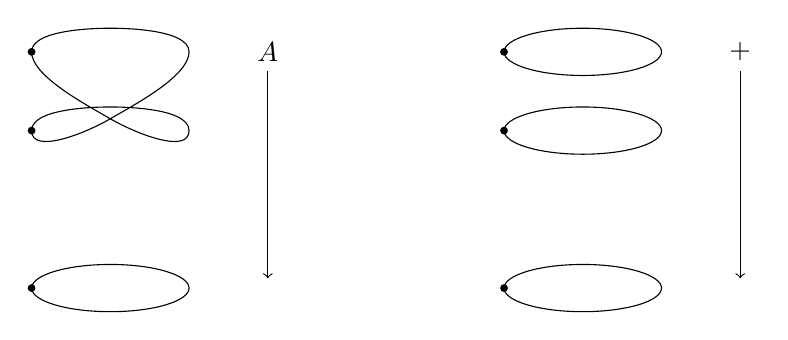
\begin{tikzpicture}
    \node (A) at (2,1) {$A$};
    \node (B) at (2,-2) {$\Sc$};
    \draw[->] (A) -- (B);
    \draw (0,-2) ellipse (1 and .3);
    \draw (-1,0)
    .. controls ++( 90:-.3) and ++(210: .4) .. (0,0.15)
    .. controls ++(210:-.4) and ++(270: .3) .. (1,1)
    .. controls ++(270:-.3) and ++(  0: .1) .. (0,1.3)
    .. controls ++(  0:-.1) and ++( 90: .3) .. (-1,1)
    .. controls ++( 90:-.3) and ++(150: .4) .. (0,0.15)
    .. controls ++(150:-.4) and ++(270: .3) .. (1,0)
    .. controls ++(270:-.3) and ++(  0: .1) .. (0,0.3)
    .. controls ++(  0:-.1) and ++( 90: .3) .. (-1,0);
    \node[fill,circle,inner sep=1pt] at (-1,-2) {};
    \node[fill,circle,inner sep=1pt] at (-1,0) {};
    \node[fill,circle,inner sep=1pt] at (-1,1) {};
%    \node (L) at (1,-3) {(left)};
    \begin{scope}[xshift=6cm]
    \node (At) at (2,1) {$\Sc+\Sc$};
    \node (Bt) at (2,-2) {$\Sc$};
    \draw[->] (At) -- (Bt);
    \draw (0,-2) ellipse (1 and .3);
    \draw (0,0) ellipse (1 and .3);
    \draw (0,1) ellipse (1 and .3);
    \node[fill,circle,inner sep=1pt] at (-1,-2) {};
    \node[fill,circle,inner sep=1pt] at (-1,0) {};
    \node[fill,circle,inner sep=1pt] at (-1,1) {};
%    \node (Lt) at (1,-3) {(right)};
    \end{scope}
  \end{tikzpicture}
  \end{sidecaption}
\end{figure}

\begin{remark}
  It \emph{is} possible to misunderstand what a ``connected \covering'' is:
the other interpretation ``all the preimages are connected''
would simply give us an equivalence (since connected sets are contractible),
and this is \emph{not} what is intended. (Equivalences are \coverings,
but not necessarily connected \coverings and connected \coverings are not neccesarily equivalences.)

Likewise for the other qualifications; for instance, in a ``finite covering'' $f:A\to B$,
the type $A$ is usually \emph{not} a finite set.

We trust the reader to keep our definitions in mind and not the other interpretations.
\end{remark}


\begin{remark}
  \Coverings are closely related to a concept from topology called ``covering spaces''
(or any variant of this concept, including Galois theory) and from algebra as locally constant sheaves (of sets).
Either way, the concept is useful because it singles out the (sub)symmetries.
\end{remark}

In this chapter, we focus on \coverings over the circle.

\begin{theorem}\label{thm:coveringsofS1perms}
  The evaluation function provides an equivalence
  \[
    \ev_\Set : (\Sc \to \Set) \to \sum_{X:\Set}(X=X)
    \quad\text{defined by $\ev_\Set(E) \defeq (E(\base),E(\Sloop))$.}
  \]
  Consequently, we have a string of equivalences
  \begin{align*}
    \SetBundle(\Sc)
    &\equiv (\Sc \to \Set)
      \equiv \sum_{X:\Set}(X=X) \\
    &\equiv \sum_{X:\Set}(X\equiv X)
    \equiv \sum_{X:\UU}\sum_{f:X\to X}
    \isset(X) \times \isEq(f).
  \end{align*}
\end{theorem}
\begin{proof}
  The first part is the universal property of the circle,
  \cref{lem:freeloopspace}, applied to $A\defeq\Set$.
  The equivalences then follow from \cref{lem:Prop-Set-pointed-families}\ref{lem:Set-families} and the univalence axiom,
  together with minor manipulations.
\end{proof}
In slogan form: A \covering over the circle is a set with a permutation of its elements.
The fiber over $\base:\Sc$ gives the set,
and transporting along $\Sloop$ gives the permutation.

A particularly important example is the following:
\begin{definition}\label{def:RtoS1}
  The \covering $R:\Sc\to\UU$ corresponds to the integers with the successor operation.
  We have $R(\base)\defeq\zet$ and $R(\Sloop)\defis \etop{\zs}$.
  (This is indeed a set bundle since $\Sc$ is connected,
  so that $R(x)$ is a set for all $x:\Sc$.
  Abusing notation we also write $R:\Sc\to\Set$.)
  Now define
  \[
    \tilde R\defeq\sum_{z:\Sc}R(z)
  \]
  and let the first projection denoted by
  \[
    \exp:\tilde R \to \Sc
  \]
  be the \emph{exponential \covering of the circle}.
\end{definition}

\begin{remark} \label{rem:expforreal}%
  \begin{marginfigure}
    \begin{tikzpicture}[scale=.15]
      \node (Sc) at (0,-5) {$\Sc$};
      \node[dot,label=left:$2$]  (B)    at (-10,18) {};
      \node[dot,label=left:$1$]  (one)  at (-10,14) {};
      \node[dot,label=left:$0$]  (zero) at (-10,10) {};
      \node[dot,label=left:$-1$] (mone) at (-10, 6) {};
      \node[dot,label=left:$-2$] (C)    at (-10, 2) {};
      \node[dot]                 (D)    at (-10,-5) {};
      \node[label=above:$\tilde R$]   (R)    at (10,20) {};
      \node[label=above left:$\zet$]  (Z)    at (-10,20) {};
      \node at (-10,20.8) {$\vdots$};
      \node at (-10,.2) {$\vdots$};
      \node[label=left:$\Sloop$] (Sloop) at (10,-5) {};

      \pgfmathsetmacro\cc{.55228475}% = 4/3*tan(pi/8)
      \pgfmathsetmacro\cy{2*\cc}%
      \pgfmathsetmacro\cx{10*\cc}%
      \pgfmathsetmacro\ay{.35165954}%

      \draw (10,0) \foreach \y in {0,4,...,16} {
        .. controls (10,\y + \cy + \ay) and (\cx,3 + \y - \ay)
        .. (0,3 + \y) .. controls (-\cx,3 + \y + \ay) and (-10,2 + \y + \cy - \ay)
        .. (-10,2 + \y) .. controls (-10,2 + \y - \cy + \ay) and (-\cx,1 + \y - \ay)
        .. (0,1 + \y) .. controls (\cx,1 + \y + \ay) and (10,4 + \y - \cy - \ay)
        .. (10,4 + \y) } ;
      \draw (10,-5) .. controls (10,-5 + \cy) and (\cx,-3)
      .. (0,-3) .. controls (-\cx,-3) and (-10,-5 + \cy)
      .. (-10,-5) .. controls (-10,-5 - \cy) and (-\cx,-7)
      .. (0,-7) .. controls (\cx,-7) and (10,-5 - \cy) .. (10,-5);
    \end{tikzpicture}
  \end{marginfigure}
  The reason for the name ``exponential'' comes from the following
  visualization.  If $x$ is a real number, then the complex
  exponentiation $\ee^{2\pi\ii x}=\cos(2\pi x)+\ii\sin(2\pi x)$ has
  absolute value $1$ and so defines a continuous function from the
  real numbers to the unit circle.  Choosing any point $z$ on the unit
  circle, we see that the preimage of $z$ under the exponential
  function is a shifted copy of the integers inside the reals.\footnote{%
    Again, we emphasize that we are here dealing with the
    \emph{homotopy types} of the reals $\RR$ and the unit circle,
    $\setof{(x,y):\RR^2}{x^2+y^2=1}$.}

  This connection between the integers and the unit circle is
  precisely captured in a form that we can take further by studying the
  \covering $\exp:\tilde R\to \Sc$.
\end{remark}

We already defined a \covering $f:A\to B$ to be universal if $A$ is connected
and all $a=_A a$ (for $a:A$) are connected.
If moreover $B$ is a pointed, connected groupoid we shall argue that
we actually can speak of \emph{the} universal \covering.

Recall \cref{cor:fib-vs-path} stating that all the fibers of a map $f:A\to B$
are sets if and only if each
\[
\ap{f}: (a=a')\to (f(a)=f(a'))
\]
is an injection.
Assume $f:A\to B$ is a universal \covering and $B$ is a groupoid.
We prove that $A$ is contractible.
Being contractible is a proposition, so we may assume
we have an element $a$ of $A$ since $A$ is connected.
By \cref{xca:connected-trivia} and \ref{xca:component-connected}
it suffices to prove that $a=a$ is contractible.
By \cref{xca:connected-trivia-2}, using that $a=a$ is connected,
it suffices to show that $a=a$ is a set.
Using that $\ap{f}$ is an injection, we can apply the remark after
\cref{lem:sum-of-fibers} and obtain that $a=a$ is a set since
$f(a)=f(a)$ is a set, since $B$ is a groupoid.
This completes the proof that $A$ is contractible.

Now assume $(B,b_0)$ is a pointed connected groupoid and $f:A\to B$
a universal \covering. Since $A$ and $\sum_{b:B}(b_0=_Bb)$ are both
contractible, and $B$ is connected, we have
$\Trunc{(A,f)=(\sum_{b:B}(b_0=_Bb),\fst)}$.
Hence if $(B,b_0)$ is a pointed connected groupoid, all
universal \coverings can be merely identified with a canonical one.
Moreover, the type of universal \coverings is equivalent to
$\bn 1 \to B$, and hence to $B$ itself,
so the type of \emph{pointed} universal \coverings is contractible.
This justifies the following definition.
\begin{definition}
  \label{def:universalcover}
  Let $(B,b_0)$ be a pointed connected groupoid.
  The \emph{universal \covering} of $B$
  is the \covering of $B$ given by the family of sets
  \[
    \uc{b_0}:B\to\Set,\quad \uc{b_0}(b)\defequi (b_0=_Bb),
  \]
  or alternatively as the first projection from
  $\uc{b_0}B\defequi\sum_{b:B}(b_0=_Bb)$ to $B$.

  This is canonically pointed at $(b_0,\refl{b_0}) : \sum_{b:B}(b_0=_Bb)$.
\end{definition}
Note that, for a general pointed connected type $(B,b_0)$, we have that
$(b_0=_B b)$ is a family of \emph{sets} exactly when $B$ is a groupoid.
The type family $(b_0=_B b)$ is also important if $B$ is not a groupoid,
but is then not a \emph{set} bundle.\footnote{%
  Of course, the type $\sum_{b:B}(b_0=b)$ is contractibe
  by \cref{lem:thepathspaceiscontractible}, for any type $B$.}

\begin{remark}
  What's so ``universal'' about this?
The universal \covering over the pointed connected groupoid $(B,b_0)$ coincides with the constant function $\cst{b_0}:\bn 1\to B$ (with value $b_0$), and seems like an unnecessary complicated representation were it not for the manifold practical value of the formulation that we've given.
In particular, we recognize the set of symmetries $b_0=_Bb_0$ as the preimage of $b_0$ under the first projection from $\uc{b_0}B$ to $B$; ultimately this will show that the study of symmetries coincides with the study of the universal \covering.

The first instance of this comes already in the next section, where we show in \cref{cor:S1groupoid} that the symmetries in the circle are given by the set of integers $\zet$ by showing that the universal \covering and the exponential \covering (\cref{def:RtoS1}) of the circle coincide.

That said, one way to see that the constant function $\cst{b_0}:\bn 1\to B$
\emph{does} deserve the label universal is the following.\marginnote{%
  Any $(a_0,p) : f^{-1}(b_0)$ gives rise to a commutative diagram:
  \[
    \begin{tikzcd}[column sep=small,ampersand replacement=\&]
      \bn 1\ar[rr,dashed,"\cst{a_0}"]\ar[dr,"\cst{b_0}"'] \& \& A \ar[dl,"f"] \\
      \& B \&
    \end{tikzcd}
  \]}
Given any function $f:A\to B$ and $(a_0,p): f^{-1}(b_0)$,
we get a function $\cst{a_0}:\bn 1\to A$, and $p:b_0=f(a_0)$ gives rise to
an element in $\cst{b_0}=_{\bn 1\to B}f \circ \cst{a_0}$.
In other words, any such $f$ is ``a factor of $\cst{b_0}$''.
Note, however, that this depends on $f^{-1}(b_0)$ being non-empty
(classically, this is often demanded of a covering, which distinguishes it from our \coverings),
and the factorization depends on the element $(a_0,p)$ used.

The situation is even simpler for pointed maps:
For any \emph{pointed} map $f : A \ptdto B$, with $(a_0,f_0):f^{-1}(b_0)$,
there is a \emph{unique} pointed map $g : \bn 1 \ptdto A$
(given by the base point of $A$), and this of course also gives
the unique way to write $f$ as a ``pointed factor of $\cst{b_0}$''.
\end{remark}

We'll continue the general study of set bundles in \cref{sec:gsets}
and indeed throughout the book.
For now, we'll focus our attention on the circle and set bundles over it.

\section{The symmetries in the circle}
\label{sec:symcirc}

With the set $\zet$ of integers \emph{defined} as in \cref{sec:integers},
we will now \emph{prove} that $\zet$ is equivalent to the type
$\base=_{\Sc}\base$, and that under this equivalence $0:\zet$ corresponds to
$\refl{\base}:\base=\base$, and $1$ to $\Sloop$, and $-1$ to $\Sloop^{-1}$.
More generally, the successor $\zs:\zet\to\zet$ corresponds to composition with $\Sloop$,
while the predecessor $\inv{\zs}$ corresponds to composition with $\Sloop^{-1}$.\marginnote{
  It follows directly that \emph{addition} of integers corresponds
  to \emph{composition} of loops.}

The first step is to prove that the exponential \covering \cref{def:RtoS1}
is equal to the universal \covering in \cref{def:universalcover},
\ie we prove that the family
\[
  R: \Sc\to\UU,\qquad R(\base)\defeq\zet,\, R(\Sloop)\defis \etop{\zs}
\]
is equal to the family
\[
\uc{\base}:\Sc\to\UU,\qquad \uc{\base}(z)\defeq (\base=z).
\]
What does it mean for the families $\uc{\base}$ and $R$ to be equal?
Type families are a special case of functions.
Function extensionality reduces the question to pointwise equality
of $\uc{\base}$ and $R$ as functions.
Using univalence, it suffices to give
an equivalence from $\uc{\base}(z)$ to $R(z)$ for every $z:\Sc$,
that is, recalling \cref{def:function-type-families},
a (fiberwise) equivalence $f: \uc{\base}\to R$. We will use
\cref{lem:weq-iso}, so will also define $g: R\to\uc{\base}$.

We first recall from \cref{sec:heavy-transport} how
transport behaves in families of function types.
Given a type $A$ and two type families $P,Q:A\to\UU$,
transport along $p:a=_Aa'$ of $h:P(a)\to Q(a)$ is
$Q(p)\,h\,P(p)^{-1}:P(a') \to Q(a')$.
In a picture,
\[
  \begin{tikzcd}[column sep=huge]
    a\ar[d,eqr,"p"] & P(a)\ar[r,"h"]\ar[d,eqr,"P(p)"] &
    Q(a)\ar[d,eqr,"Q(p)"] \\
    a' & P(a') & \,Q(a').
  \end{tikzcd}
\]
If $A$ is $\Sc$, then the induction principle for the circle says
that giving an $h(z):P(z)\to Q(z)$ for all $z:\Sc$ is the same as
specifying an $h(\base):P(\base)\to Q(\base)$ and,
using \cref{def:pathover-trp} and the discussion above, an identity
$h(\Sloop):Q(\Sloop)\,h(\base)\,P(\Sloop)^{-1}=_{P(\base)\to Q(\base)}h(\base)$,
\ie   a witness that the composites in
\[
  \begin{tikzcd}[column sep=huge]
    P(\base)\ar[r,"h(\base)"]\ar[d,eqr,"P(\Sloop)"]
    & Q(\base)\ar[d,eqr,"Q(\Sloop)"] \\
    P(\base)\ar[r,"h(\base)"] & Q(\base)
  \end{tikzcd}
\]
are equal. If $P,Q$ are families of sets,
then the type of $h(\Sloop)$ is a proposition.

We now define $f: \uc{\base}\to R$ and $g: R\to\uc{\base}$ that will turn out to
give inverse equivalences between $\uc{\base}(z)$ and $R(z)$, for each $z:\Sc$.

\begin{marginfigure}
  \begin{tikzpicture}[scale=.15]
    \node (Sc) at (0,-5) {$\Sc$};
    \node[dot,label=above:$\vdots$] (B)    at (-10,18) {};
    \node[dot]                      (one)  at (-10,14) {};
    \node[dot]                      (zero) at (-10,10) {};
    \node[dot]                      (mone) at (-10, 6) {};
    \node[dot]                      (C)    at (-10, 2) {};
    \node[dot]                      (D)    at (-10,-5) {};
    \node[label=above:$\RR$]        (R)    at (10,20) {};
    \node[label=above left:$\zet$]  (Z)    at (-10,20) {};
    \node at (-10,.2) {$\vdots$};
    \node[label=left:$\Sloop$] (Sloop) at (10,-5) {};

    \pgfmathsetmacro\cc{.55228475}% = 4/3*tan(pi/8)
    \pgfmathsetmacro\cy{2*\cc}%
    \pgfmathsetmacro\cx{10*\cc}%
    \pgfmathsetmacro\ay{.35165954}%

    \draw (10,0) \foreach \y in {0,4,...,16} {
      .. controls (10,\y + \cy + \ay) and (\cx,3 + \y - \ay)
      .. (0,3 + \y) .. controls (-\cx,3 + \y + \ay) and (-10,2 + \y + \cy - \ay)
      .. (-10,2 + \y) .. controls (-10,2 + \y - \cy + \ay) and (-\cx,1 + \y - \ay)
      .. (0,1 + \y) .. controls (\cx,1 + \y + \ay) and (10,4 + \y - \cy - \ay)
      .. (10,4 + \y) } ;
    \draw (10,-5) .. controls (10,-5 + \cy) and (\cx,-3)
    .. (0,-3) .. controls (-\cx,-3) and (-10,-5 + \cy)
    .. (-10,-5) .. controls (-10,-5 - \cy) and (-\cx,-7)
    .. (0,-7) .. controls (\cx,-7) and (10,-5 - \cy) .. (10,-5);

    \draw[->, bend left, shorten <=2pt, shorten >=2pt] (zero) to
    node[left] {\scriptsize$\trp[R]{\Sloop}$} (one);%
    \draw[->, bend right, shorten <=2pt, shorten >=2pt] (zero) to
    node[left] {\scriptsize$\trp[R]{\inv\Sloop}$} (mone);%
    \draw[->, bend right, shorten <=2pt, shorten >=2pt, line
    width=2pt, white] (zero) to (B);%
    \draw[->, bend right, shorten <=2pt, shorten >=2pt] (zero) to
    node[right,rounded corners,fill=white,outer sep=5pt]
    {\scriptsize$\trp[R]{\Sloop^2}$} (B);%
    \draw[->, bend left, shorten <=2pt, shorten >=2pt, white, line
    width=2pt] (zero) to (C);%
    \draw[->, bend left, shorten <=2pt, shorten >=2pt] (zero) to
    node[right,rounded corners,fill=white,outer sep=5pt]
    {\scriptsize$\trp[R]{\Sloop^{-2}}$} (C);
  \end{tikzpicture}
  \caption{Transport in the family $R$}\label{fig:transportalongloop}
\end{marginfigure}
\begin{definition}
  \label{def:fPtoR}
  The function $f:\prod_{z:\Sc}(\uc{\base}(z)\to R(z))$ is defined by transport: $f(z)(p)\defequi\trp[R]{p}(0)$.
\end{definition}
In Figure~\ref{fig:transportalongloop}, the transport in the definition
above has been visualised for $p={\Sloop^n}$, $n=-2,-1,0,1,2$.

\begin{lemma}\label{lem:windingnumber}
For $f$ as in \cref{def:fPtoR} we have $f(\base)(\Sloop^n)=n$ for all $n:\zet$.
\end{lemma}
\begin{proof}
First consider positive $n:\NN$ and apply induction. In the base case $n=0$ we have
$f(\base)(\Sloop^0)\jdeq f(\refl\base)\jdeq\trp[R]{\refl\base}(0) \jdeq 0$.
For $n=\zs(m)$ with $m:\NN$ we have
\begin{align*}
  f(\base)(\Sloop^{\zs(m)})
  &\jdeq\trp[R]{\Sloop^{\zs(m)}}(0)\\
  &=\trp[R]{\Sloop \Sloop^{m}}(0)\\
  &=\trp[R]{\Sloop}(\trp[R]{\Sloop^m}(0))\\
  &\jdeq \trp[R]{\Sloop}(f(\base)(\Sloop^{m}))\\
  &= \zs(f(\base)(\Sloop^{m})).
\end{align*}
The last step follows from $\etop{\zs}=R(\Sloop)$
and $\zs=\trp[\id_\UU]{\etop{\zs}}$, see \cref{def:univalence},
and hence $\zs=\trp[\id_\UU]{R(\Sloop)}=\trp[\id_\UU R]{\Sloop}=\trp[R]{\Sloop}$.
This completes the induction step for positive $n$.
For negative $n$ the proof is similar.
\end{proof}

In the definition of the second map,
take into account that $R(\base)\jdeq \zet$ and $\uc{\base}(\base) \jdeq (\base=\base)$.

\begin{definition}\label{def:gRtoP}
The function $g:\prod_{z:\Sc}(R(z)\to \uc{\base}(z))$ is
defined by circle induction:
\[
g(\base)\defeq \left(n \mapsto {\Sloop^n} \right) :\zet\to(\base=\base)
\]
and
\[
g(\Sloop): \uc{\base}(\Sloop)\, g(\base)\,R(\Sloop)^{-1}=_{\zet\to (\base=\base)} g(\base).
\]
\marginnote{%
  In a picture, $g(\Sloop)$ should prove that it does not matter what
  path you take around the square
  \[
    \begin{tikzcd}[row sep=large,column sep=huge,ampersand replacement=\&]
      \zet\ar[r,"\Sloop^-"]\ar[d,eqr,"\zs"] \&
      (\base=\base)\ar[d,eqr,"\Sloop\cdot\blank"] \\
      \zet\ar[r,"\Sloop^-"] \& (\base=\base).
    \end{tikzcd}
  \]
}%
So far we have only given the type of $g(\Sloop)$. By definition,
$R(\Sloop)$ is $\zs$ and $\uc{\base}(\Sloop)$ is composition with
$\Sloop$.
The element $g(\Sloop)$ follows by a simple calculation: the
proposition ${\Sloop\,\Sloop^{n-1}} = {\Sloop^n}$ holds for all
$n:\zet$.
\end{definition}


\begin{theorem}
  \label{lem:univisexp}
For every $z:\Sc$, the functions $f(z)$ defined in \cref{def:fPtoR}
and $g(z)$ in \cref{def:gRtoP} are inverse equivalences between
$\uc{\base}(z)$ and $R(z)$.
\end{theorem}
\begin{proof}
We apply \cref{lem:weq-iso} and verify the two conditions.
  First, we need to give elements $H(z,p):g(z)(f(z)(p))=p$
for all $z:\Sc$ and $p:\uc{\base}(z)\jdeq(\base=z)$.
By induction on $p:\base=z$ it suffices to set
$H(\base,\refl\base)\defeq\refl{\refl{\base}}$ since
$g(\base)(f(\base)(\refl{\base}))\jdeq g(\base)(0)\jdeq\refl{\base}$.

Secondly, we need to give elements $G(z)(n):f(z)(g(z)(n))=n$
for all $z:\Sc$ and $n: R(z)$.
By circle induction it suffices to define $G(\base)$ and $G(\Sloop)$,
but since $\zet$ is a set the information for $G(\Sloop)$ is redundant.
Hence, we need to show that for all $n:\zet$ that
$f(\base)(g(\base)(n))\jdeq  f(\base)(\Sloop^n)$ is equal to $n$.
This follows from \cref{lem:windingnumber}.
\end{proof}


\begin{corollary}\label{cor:S1groupoid}
The circle $\Sc$ is a groupoid, and the function
\[
{\Sloop}^{\blank} : \zet\to(\base=_{\Sc}\base)
\]
sending $n$ to $\Sloop^n$ is an equivalence.
\end{corollary}
\begin{proof}
For any $z:\Sc$, the type $\uc{\base}(z)\jdeq (\base=_{\Sc}z)$ is a set
since $R(z)$ is a set and $\uc{\base}(z) \equiv R(z)$.
Since the circle is connected and being a set is a proposition, it follows
that $y=_{\Sc}z$ is a set, for any $y,z:\Sc$. Hence $\Sc$ is a groupoid.
By \cref{def:gRtoP}, ${\Sloop}^{-}\jdeq g(\base)$ is an equivalence.
\end{proof}
\begin{definition}\label{def:windingnumber}
  The inverse function of ${\Sloop}^{\blank}$
  is called the \emph{winding number} function
  $\wdg : (\base =_\Sc\base) \to \zet$.
\end{definition}
The following lemma is a simple example of a technique later called \emph{delooping}.
\begin{lemma}\label{lem:S1-delooping}
Let $A$ be a connected type and $a:A$.
Assume we have an equivalence $e:(\base=_{\Sc}\base) \to (a=a)$
of symmetries such that $e(\refl{\base})=\refl{a}$
and $e(p\cdot q)=e(p)\cdot e(q)$, for all $p,q:(\base=_{\Sc}\base)$.
Then $\check e : \Sc\to A$ defined by circle recursion by setting
$\check e(\base)\defeq a$ and $\check e(\Sloop)\defis e(\Sloop)$
is an equivalence.
\end{lemma}
\begin{proof}
We have $\ap{\check e} = e$ since they produce equal values when applied
to $\Sloop^n$, for all $n:\zet$. Now use that $A$ and $\Sc$ are connected and
apply \cref{cor:fib-vs-path}\ref{conn-fib-vs-path}.
\end{proof}

\begin{xca}\label{xca:general-winding}
  Generalizing~\cref{def:windingnumber}, of winding numbers,
  use circle induction to define, for any point $x:\Sc$ of the circle
  an equivalence, $\wdg_x : (x =_\Sc x) \we \zet$.
  (You'll need commutativity of addition in $\zet$.)
  Conclude from \cref{lem:S1-delooping} that we have equivalences
  $f_x : \Sc \we \Sc$ with $f_x(\base) \jdeq x$, for each $x:\Sc$.\footnote{%
    If we think of the circle as represented by the unit length complex numbers,
    then $f_x(y)$ corresponds to the usual product $xy$.}
\end{xca}

\begin{xca}\label{xca:S1=S1-components}
Let $-\id_\Sc : \Sc\to\Sc$ be defined by $-\id_\Sc(\base)\defeq\base$
and $-\id_\Sc(\Sloop)\defis{\Sloop}^{-1}$. Show the $-\id_\Sc$
and $\id_\Sc$ are not in the same component of $\Sc\to\Sc$.
Prove the following proposition:
\[
\prod_{t:\Sc\equiv\Sc}{\Trunc{\id_\Sc\eqto t}\amalg \Trunc{-\id_\Sc\eqto t}}.\qedhere
\]
\end{xca}

\begin{xca}\label{xca:(S1->S1)_(f)-eqv-S1}
For any $f: \Sc\to\Sc$, give an equivalence
from $\Sc$ to $(\Sc\to\Sc)_{(f)}$, that is, from $\Sc$ to
the component of $\Sc\to\Sc$ at $f$.
Hint: use \cref{lem:S1-delooping}.
\end{xca}

We note in passing that combining the above two exercises
yields an equivalence from $(\Sc\eqto\Sc)$ to $(\Sc\amalg\Sc)$,
that is, a characterization of the symmetries \emph{of} the cycle
(in constrast to the title of this \cref{sec:symcirc}).


\section{A reinterpretation of the circle}\label{sec:S1isC}

In this section we return to the equivalences in \cref{thm:coveringsofS1perms}.
We'll use these to get a different perspective on the circle,
which highlights it as a type classifying very simple symmetries,
namely sets with permutations.
We have already seen one example in \cref{def:RtoS1},
namely the set $\zet$ of integers together with the successor $\zs: \zet\equiv\zet$,
corresponding to the universal \covering $\uc\base:\Sc \to \Set$,
which as a map is the constant function $\cst\base : \bn 1 \to \Sc$.

The importance of the latter example will become apparent when we eventually
explain that \emph{the circle is equivalent to the connected component of
  $(\zet,\zs)$ in the type $\sum_{X:\UU}(X\to X)$}.\footnote{%
  The elements of this connected component can be thought of as
  \emph{infinite cycles}:
  sets $X$ with a successor function $t:X \to X$
  such that $(X,t)$ can be merely identified with $(\zet,\zs)$.
  That is, $(X,t)$ looks exactly like $(\zet,\zs)$,
  but we don't know which element of $X$ is ``zero'':\\[1ex]
  \begin{tikzpicture}[node distance=10pt]
    \begin{scope}[every node/.style={dot}]
      \node (x1) {};
      \foreach \p/\n/\deg in {1/2/27, 2/3/54, 3/4/81, 4/5/108, 5/6/135,%
        6/7/162, 7/8/135, 8/9/108, 9/10/81, 10/11/54, 11/12/27} {
        \node (x\n) [at=(x\p.\deg), anchor=\deg+180, shift=(\deg:10pt)] {};
      }
    \end{scope}
    \node (x0) [left=of x1] {$\ldots$};
    \node (x13) [right=of x12] {$\ldots$};
    \begin{scope}[->,shorten <=1pt,shorten >=1pt]
      \foreach \p/\n in {0/1, 1/2, 2/3, 3/4, 4/5, 5/6,
        6/7, 7/8, 8/9, 9/10, 10/11, 11/12, 12/13} {
        \draw (x\p)--(x\n);
      }
    \end{scope}
  \end{tikzpicture}}

The key of course is that the equivalences in \cref{thm:coveringsofS1perms}
restrict to equivalences between their connected components,
so to understand the components of $\SetBundle(\Sc)$
it suffices to understand the components of $\sum_{X:\UU}(X \to X)$ at pairs $(X,t)$,
where $X$ is a set with a permutation $t$.

We are particularly interested in understanding the symmetries in these components,
so before we prove that the circle is equivalent to the component containing $(\zet,\zs$),
let us investigate the equalities in the type $\sum_{X:\UU}(X \to X)$ a bit further.

Define the type family $D$ by $D(X) \defeq (X\to X)$ for all $X:\UU$.
Recall from \cref{lem:isEq-pair=} that, given $X,Y:\UU$ and $t:X\to X$ and $u:Y\to Y$,
the identity type $(X,t)=(Y,u)$
is equivalent to the type of pairs consisting of a $p:X=Y$ and
an element of $\pathover{t}{D}{p}{u}$. The latter type is
equivalent to $\trp[D]{p}(t) = u$ by \cref{def:pathover-trp}.
The transport is by conjugation,
\cref{lem:trp-in-function-type}, so that the latter
type is equivalent to $\ptoe p\circ t\circ \ptoe p^{-1} = u$.
If $p\jdeq\etop e$ for an equivalence $e:X\equiv Y$,
this is equivalent to $e\circ t = u\circ e$, or $e t = u e$ for short.
In total, the identity type $(X,t)=(Y,u)$ is equivalent to
\[
  \sum_{e: X\equiv Y} et =_{X\to Y} ue.
\]
This is a set whenever $X$ and $Y$ are; see \cref{fig:Zs=Xt} for an illustration.
\begin{marginfigure}
  \begin{tikzpicture}[node distance=10pt]
    \begin{scope}[every node/.style={dot}]
      \node (x1) {};
      \foreach \p/\n/\deg in {1/2/72, 2/3/54, 3/4/81, 4/5/108, 5/6/135,%
        6/7/162, 7/8/135, 8/9/108, 9/10/81, 10/11/54, 11/12/72} {
        \node (x\n) [at=(x\p.\deg), anchor=\deg+180, shift=(\deg:10pt)] {};
      }
      \node (y1) [at=(x1.east), anchor=180, shift=(192:50pt)] {};
      \foreach \p/\n in {1/2, 2/3, 3/4, 4/5, 5/6,%
        6/7, 7/8, 8/9, 9/10, 10/11, 11/12} {
        \node (y\n) [at=(y\p.north), anchor=south, shift=(90:10pt)] {};
      }
    \end{scope}
    \node (x0) [below=of x1] {$\vdots$};
    \node (y0) [below=of y1] {$\vdots$};
    \node (x13) [above=of x12] {$\vdots$};
    \node (y13) [above=of y12] {$\vdots$};
    \node (Xf)  [above=26pt of x12] {$(X,t)$};
    \node (Zs)  [left=2pt of y13] {$(\zet,\zs)$};
    \node (zero)  [left=2pt of y6] {$0$};
    \begin{scope}[->,shorten <=1pt,shorten >=1pt]
      \foreach \p/\n in {0/1, 1/2, 2/3, 3/4, 4/5, 5/6,
        6/7, 7/8, 8/9, 9/10, 10/11, 11/12, 12/13} {
        \draw (x\p)--(x\n);
        \draw (y\p)--(y\n);
      }
    \end{scope}
    \begin{scope}[casblue,<-,shorten <=1pt,shorten >=1pt]
      \foreach \n in {1,2,...,12} {
        \draw (x\n)--(y\n);
      }
    \end{scope}
  \end{tikzpicture}
  \caption{An identification of two infinite cycles.
    The equivalence $e : \zet \equiv X$ is marked in blue.}\label{fig:Zs=Xt}
\end{marginfigure}
In particular, the identity type $(\zet,\zs)=(X,t)$
is equivalent to the set $\sum_{e:\zet\equiv X}e\zs=te$, for any set $X$ with a permutation $t$.
Tautologically, then, any power $\zs^n$ of $\zs$ itself gives a symmetry
$(\zs^n,!) : (\zet,\zs)=(\zet,\zs)$.

The following property jumps out at us when we contemplate~\cref{fig:Zs=Xt}.
\begin{lemma}
  \label{lem:IdCisZet}
  An element $(e,!) : (\zet,\zs)=(X,t)$,
  with $(X,t)$ in the component of $(\zet,\zs)$,
  is uniquely determined by the element $e(0):X$.
  In other words, the function
  \[
    \ev_0:\bigl((\zet,\zs)=(X,t)\bigr)\to X
    \text{~~defined by~~} \ev_0(e,!) \defeq e(0)
  \]
  is an equivalence.
\end{lemma}
\begin{proof}
  We'll prove that every fiber of $\ev_0$ is contractible.
  Given $x_0:X$ we must determine a unique equivalence $e:\zet\to X$
  such that $es=te$ and $e(0)=x_0$.
  Induction on $n:\zet$ (positive and negative $n$ separately)
  shows that for such an $e$, we have $e(n) = t^n(x_0)$ for all $n:\zet$.
  It remains to prove that this is an equivalence.
  More precisely, it suffices to prove the proposition:
  \begin{displaymath}
    \prod_{x_0:X} \isEq(n\mapsto t^n(x_0))
  \end{displaymath}
  Since we are proving a proposition,
  and we are assuming $(X,t)$ is in the component of $(\zet,\zs)$,
  it suffices to prove it for $(X,t) \jdeq (\zet,\zs)$.
  However, for any $x_0:\zet$,
  the map $n \mapsto \zs^n(x_0) = n + x_0$ is an equivalence,
  with inverse $n \mapsto n - x_0$.
\end{proof}
In particular, the identity type $(\zet,\zs)=(\zet,\zs)$ is equivalent to $\zet$.

\begin{definition}\label{def:S1toC}
  Let $\InfCyc$ be the component of $\sum_{X:\UU}(X\to X)$ containing $(\zet,\zs)$.
  Elements of $\InfCyc$ are called \emph{infinite cycles}.\footnote{%
    See also~\cref{def:Cyc} below for general cycles.}

  Define by circle induction
  \[
    c:\Sc\to\InfCyc \text{~~setting~~}
    c(\base)\defequi (\zet,\zs)
  \]
  and $c(\Sloop): c(\base)= c(\base)$ given by the \emph{predecessor} equivalence
  $\zs^{-1}:\zet\to\zet$
  and the trivial proof of the proposition $\zs^{-1}\zs=\zs\zs^{-1}$.
\end{definition}
\begin{marginfigure}
  \noindent\begin{tikzpicture}[scale=.15]
    \node (Sc) at (0,-5) {$\Sc$};
    \node[dot]                 (D)    at (-10,-5) {};
    \node[label=above left:$\uc{\color{casred}\base}({\color{casblue}\base})$] (Z) at (-10,20) {};
    \node at (-10,24.8) {$\vdots$};
    \node at (-10,.2) {$\vdots$};
    \node[label=left:$\Sloop$] (Sloop) at (10,-5) {};

    \pgfmathsetmacro\cc{.55228475}% = 4/3*tan(pi/8)
    \pgfmathsetmacro\cy{2*\cc}%
    \pgfmathsetmacro\cx{10*\cc}%
    \pgfmathsetmacro\ay{.35165954}%

    \draw[dashed] (10,0)
    .. controls (10,\cy + \ay) and (\cx,3 - \ay)
    .. (0,3) .. controls (-\cx,3 + \ay) and (-10,2 + \cy - \ay)
    .. (-10,2);
    \foreach \y/\col in {0/dashed,4/casred,8/black,12/casblue,16/dashed} {
      \draw[\col] (-10,2 + \y)
      .. controls (-10,2 + \y - \cy + \ay) and (-\cx,1 + \y - \ay)
      .. (0,1 + \y) .. controls (\cx,1 + \y + \ay) and (10,4 + \y - \cy - \ay)
      .. (10,4 + \y) .. controls (10,4 + \y + \cy + \ay) and (\cx,7 + \y - \ay)
      .. (0,7 + \y) .. controls (-\cx,7 + \y + \ay) and (-10,6 + \y + \cy - \ay)
      .. (-10,6 + \y);
    }
    \draw[dashed] (-10,22)
    .. controls (-10,22 - \cy + \ay) and (-\cx,21 - \ay)
    .. (0,21) .. controls (\cx,21 + \ay) and (10,24 - \cy - \ay)
    .. (10,24);
    \foreach \y in {2,6,...,22} {
      \node[dot] (B\y) at (-10,\y) {};
    }
    \draw (10,-5) .. controls (10,-5 + \cy) and (\cx,-3)
    .. (0,-3) .. controls (-\cx,-3) and (-10,-5 + \cy)
    .. (-10,-5) .. controls (-10,-5 - \cy) and (-\cx,-7)
    .. (0,-7) .. controls (\cx,-7) and (10,-5 - \cy) .. (10,-5);
  \end{tikzpicture}
  \caption{For the fiber of the universal \covering,
    $\uc{\color{casred}\base}({\color{casblue}\base}) \jdeq
    ({\color{casred}\base} = {\color{casblue}\base})$,
    we \emph{increase} the winding number when we transport
    the endpoint (in blue) along $\Sloop$, and
    we \emph{decrease} it when we transport the starting point
    (in red) in the same way.}\label{fig:plus-minus-one}
\end{marginfigure}

Note that, as usual, we leave out the propositional components of $\InfCyc$ (and other subtypes) from the notation.

Since it's such a crucial result, we are going to give two proofs that $c$ from \cref{def:S1toC} is an equivalence.
Each proof illuminates a different aspect and gives methods that will be used later.

For the first, we return to the equivalences of \cref{thm:coveringsofS1perms}.
As we said above, these restrict to equivalences between the different components.
In particular, $\ev_\UU : (\Sc \to \UU) \to
\sum_{X:\UU}X=X$ maps the type family $\uc{\base}$ to the pair
$(\base = \base, q\mapsto {{\Sloop}\cdot q})$,
which can be identified with $(Z,s)$ through~\cref{cor:S1groupoid}.
Hence, $\ev_\UU$ restricts to an equivalence between the
connected component of $\uc\base$ in $\Sc \to \UU$ and the connected component
of $(Z,s)$ in $\sum_{X:\UU}X=X$.
We claim that we get a commuting diagram
\begin{equation}\label{eq:setbundle-Sc-univ-comp}
  \begin{tikzcd}
    & \Sc\ar[dl,"\cst{\blank}"']\ar[d,"\uc{\blank}"]\ar[dr,"c"] & \\
    \conncomp{\SetBundle(\Sc)}{\cst\base} \ar[r,"\sim"]
    & \conncomp{(\Sc\to\UU)}{\uc\base} \ar[r,"\sim","\ev_\UU"']
    & \InfCyc,
  \end{tikzcd}
\end{equation}
where the left-most diagonal arrow maps $z:\Sc$ to the constant map $\cst z:\bn 1\to\Sc$.
The left-hand triangle commutes, because the fiber $\sum_{\_:\bn 1}(x=z)$
of $\cst z$ at $x:\Sc$ is equivalent to $\uc{z}(x) \jdeq (z=x)$.
We prove that the right-hand triangle commutes by circle induction.
That is, we show $\prod_{z:\Sc}c(z) = \ev_\UU(\uc{z})$.
The case $z\jdeq\base$ is exactly the equivalence
$g(\base)\jdeq{\Sloop^-} : \zet \to \uc{\base}(\base)$ of \cref{lem:univisexp}
together with the fact that $\trp[\uc\base]{\Sloop}$ corresponds to $\zs$.
To finish, we observe that it doesn't matter which way you take in the diagram
\[
  \begin{tikzcd}[row sep=large,column sep=huge]
    \zet\ar[r,"\Sloop^-"]\ar[d,"\inv{\zs}"] &
    (\base=\base)\ar[d,"\blank\cdot\Sloop^{-1}"] \\
    \zet\ar[r,"\Sloop^-"] & (\base=\base).
  \end{tikzcd}
\]
Note that to transport in the family $\uc{-}(\base) \jdeq (\blank = \base)$,
we use \cref{xca:trp-in-a/x=b/x}\ref{trp-in-x=a},
and \emph{that} is why we picked the predecessor equivalence in~\cref{def:S1toC}.
This is also illustrated in \cref{fig:plus-minus-one}.\footnote{%
  Another option would have been to choose the opposite equivalence $\zet\equiv\uc\base(\base)$, sending $n$ to $\Sloop^{-n}$, in the base case.
  The point is: You can move the minus sign around, but it has to pop up somewhere.}

With~\eqref{eq:setbundle-Sc-univ-comp} in hand, we see that $c$ is an equivalence
if and only if either of the two other downward maps are.\footnote{%
  At this point we could conclude with an appeal to the type theoretic Yoneda lemma,
  which states that the map $X \to (X \to \UU)$,
  sending $x$ to the family $y \mapsto x=y$,
  is an injection for any type $X$.
  Exercise: Prove this!}
It is very direct to show that the map on the left is an equivalence.
Indeed, the identity type $(\bn 1,\cst x)=(\bn 1,\cst y)$
is equivalent to pairs of an equivalence $e : \bn 1 \to \bn 1$ and a commuting triangle
\[
  \begin{tikzcd}
    \bn 1 \ar[rr,"e"]\ar[dr,"\cst x"'] & & \bn 1\ar[dl,"\cst y"] \\
    & \Sc. &
  \end{tikzcd}
\]
But since $\bn 1$ is contractible, this just amounts to the equality $x=y$.
Hence the map is an embedding, and we conclude by \cref{cor:fib-vs-path}\ref{conn-fib-vs-path}.

We now give the second, more direct, proof that $c$ is an equivalence.
For this we use the following lemma, which is of independent interest.
\begin{lemma}\label{lem:conn-eq-f-ap-f-x}
Let $X$ and $Y$ be connected types, $x$ an element of $X$,
and $f$ a function from $X$ to $Y$. Then $f$ is an equivalence
if and only if $\ap{f}: (x=x) \to (f(x)=f(x))$ is an equivalence.
\end{lemma}
\begin{proof}
Using \cref{cor:fib-vs-path}\ref{conn-fib-vs-path} it suffices to show that
each map induced by $f$ on identity types is an equivalence if and only if the specific map
$\ap f : (x=x) \to (f(x) = f(x))$ is an equivalence.  Being an equivalence is a proposition,
so the result follows in two easy steps from $X$ being connected,
using \cref{xca:component-connected}.
\end{proof}

\begin{theorem}\label{thm:S1bysymmetries}
  The function $c:\Sc\to\InfCyc$ from \cref{def:S1toC} is an equivalence.
\end{theorem}
\begin{proof}
  In view of \cref{lem:conn-eq-f-ap-f-x} we only need to show that
$\ap{c}:(\base=_{\Sc}\base)\to((\zet,\zs)=(\zet,\zs))$ is an equivalence.
Note that both the domain and the co-domain of $\ap{c}$ are equivalent to $\zet$.
Consider the following diagram in which we compose $c$ with the equivalences
from \cref{cor:S1groupoid} and \cref{lem:IdCisZet}:
\[
  \begin{tikzcd}[column sep=large]
    \zet\ar[r,"\Sloop^-"] &
    (\base=\base)\ar[r,"\ap{c}"] &
    \bigl((\zet,\zs)=(\zet,\zs)\bigr)\ar[r,"\ev_0\vphantom{\ap{c}}"] &
    \zet
  \end{tikzcd}
\]
For $c$ to be an equivalence, it suffices to show that the composition
is an equivalence from $\zet$ to itself.
By definition, $\ap{c}(\Sloop)$ is the identification
corresponding to $\inv\zs$, sending $0$ to $-1$,
and by induction on $n:\zet$ it follows that
$\ev_0(\ap{c}(\Sloop^n)) = \zs^{-n}(0) = -n$.
And the map $n \mapsto -n$ is indeed an equivalence.
\end{proof}

\section{Connected \coverings over the circle}
\label{sec:covS1}

Let $A$ be a type and $f:A\to \Sc$ a function.
By \cref{cor:fib-vs-path}\ref{set-fib-vs-path}, $f$ is a \covering
over $\Sc$ if and only if each map induced by $f$ on identity types is injective.
Assume that $f:A\to \Sc$ is a \covering with $A$ connected.
Let $(a_0,p)$ be an element of $f^{-1}(\base)$.
By \cref{xca:component-connected}
the condition that \emph{each} $\ap{f}$ is injective
can be relaxed to $\ap{f}: (a_0=a_0)\to(f(a_0)=f(a_0))$ being injective.
Now look at the following subset:
\begin{equation}\label{eq:subgroup-covering-1}
  \setof{q: \base =_\Sc \base}{{\ap{f}}^{-1}(pqp^{-1})}.
\end{equation}
Clearly, a classification of connected \coverings over the circle
also classifies certain subsets of symmetries of $\base$,
or equivalently, using~\cref{cor:S1groupoid}, certain subsets of $\zet$.
Such subsets of $(\base=_\Sc\base)$ are closed under concatenation and inverses,
since $\ap{f}$ is compatible with these operations,
see \cref{lem:apcomp}.
Using language yet to be introduced, we actually ``classify the subgroups of the integers''.

Recall that \coverings over the circle are equivalent to sets with permutations.
Which sets with permutations $(X,t)$ correspond to connected \coverings?
It is not so surprising that the answer has to do with whether
any two points $x,x':X$ can be connected by applying $t$ some number of times.
\begin{definition}\label{def:Cyc}
  Let $\Cyc$ be the subtype of $\sum_{X:\UU}(X\to X)$ of those
  pairs $(X,t)$ where $X$ is a \emph{\nonempty} set with an \emph{equivalence} $t$
  such that for any $x,x':X$
  there exists some $n:\zet$ with $x' = t^n(x)$.\marginnote{%
    Recall that the iteration $t^n$ makes sense for all integers $n$
    since $t$ is an equivalence.}
  Elements of $\Cyc$ are called \emph{cycles}.\footnote{%
    Our cycles are a special case of what is elsewhere called
    \emph{cyclically ordered sets},
    and they are closely related to the \emph{cyclic sets} of
    \citeauthor{Connes1983}\footnotemark{}.}\footcitetext{Connes1983}
\end{definition}
\begin{theorem}\label{thm:cycset-connS1cover}
  Under the equivalence of \cref{thm:coveringsofS1perms},
  connected \coverings of the circle correspond to cycles.
\end{theorem}
\begin{proof}
  Consider a set $X$ with permutation $t$.
  The corresponding family of sets is $E\defeq\ve_\UU(X,\etop{t}) : \Sc\to\UU$,
  so the corresponding set bundle over the circle
  is the first projection, $\fst : A \to \Sc$,
  where we put $A\defeq\sum_{z:\Sc}E(z)$.
  We need to show that $A$ is connected if and only if $X$ is \nonempty
  and any two elements of $X$ can be connected by $t$.

  We show something a little more general, namely we give a bijection
  $g : \setTrunc A \to X/\sim$, from the set of components of $A$
  to the quotient set of $X$ by the equivalence relation $\sim$
  defined by $(x\sim x') \defeq \exists_{n:\zet}(x'=t^n(x))$.\footnote{%
    Exercise: Check that this defines an equivalence relation,
    and that the bijection $g$ proves the theorem.}

  We define $g$ using the universal property of set truncation (\cref{def:set-truncation}), pair induction, and circle induction.
  To define $g_0 : \prod_{z:\Sc}(E(z) \to X/\sim)$, we need
  $g_0(\base)\defeq[\blank] : X \to X/\sim$ and
  $g_0(\Sloop) : \pathover{g_0(\base)}{E(\blank) \to X/\sim}{\Sloop}{g_0(\base)}$,
  equivalent to $g_0(\base) =_{X \to X/\sim} g_0(\base)t$.
  The latter we get by function extensionality and \cref{thm:quotient-property},
  since $x \sim t(x)$ for any $x:X$.

  The inverse of $g$, $h:(X/\sim) \to \setTrunc A$,
  is defined as the extension of $h_0 : X \to \setTrunc A$
  with $h_0(x) \defeq \settrunc{(\base,x)}$.
  We just need to check that $h_0(x) = h_0(x')$, or equivalently,
  $\Trunc{(\base,x)=_A(\base,x')}$, whenever $x\sim x'$.
  Since this is a proposition, if $x'=t^n(x)$ with $n:\zet$,
  we may use induction on $n$ (positive and negative)
  together with the paths,
  $\pathpair{\Sloop}{\refl{f(x)}} : (\base,x)=(\base,t(x))$,
  to conclude.

  It's easy to check that $g$ and $h$ are mutually inverse.
\end{proof}
In \cref{fig:two-comp-S1-cover} we see the \covering corresponding
to the set $\set{1,2,3,4,5}$ with the permutation $1\mapsto 2\mapsto 3\mapsto 1,4\mapsto 5\mapsto 4$. There are two components, showing that the permutation splits into two cycles.
\begin{marginfigure}
  \begin{tikzpicture}[scale=.15]
    \node (Sc) at (0,-5) {$\Sc$};
    \node[dot,label=left:$5$] (four)  at (-10,22) {};
    \node[dot,label=left:$4$] (three) at (-10,18) {};
    \node[dot,label=left:$3$] (two)   at (-10,10) {};
    \node[dot,label=left:$2$] (one)   at (-10, 6) {};
    \node[dot,label=left:$1$] (zero)  at (-10, 2) {};
    \node[dot]                (D)     at (-10,-5) {};
    \node[label=left:$\Sloop$] (Sloop) at (10,-5) {};

    \pgfmathsetmacro\cc{.55228475}% = 4/3*tan(pi/8)
    \pgfmathsetmacro\cy{2*\cc}%
    \pgfmathsetmacro\cx{10*\cc}%
    \pgfmathsetmacro\intx{3.5}%
    \pgfmathsetmacro\inty{1.5}%
    \pgfmathsetmacro\ay{.35165954}%

    \draw (-10,18) .. controls (-10,18 - \cy + \ay) and (-\cx,17 - \ay)
    .. (0,17) .. controls (\cx,17 + \ay) and (10,20 - \cy - \ay) .. (10,20)
    .. controls (10,20 + \cy + \ay) and (\cx,23 - \ay)
    .. (0,23) .. controls (-\cx,23 + \ay) and (-10,22 + \cy - \ay)
    .. (-10,22) .. controls (-10,22 - \cy + \ay) and (-\cx,21 - \ay)
    .. (0,21) .. controls (\cx,21 + \ay) and (10,24 - \cy - \ay)
    .. (10,24)
    .. controls (10,24 + \cc) and (\intx + \cx, 24 + \inty + \ay)
    .. (\intx,24 + \inty) .. controls (\intx - \cx,24 + \inty - \ay)
    and (-\intx + \cx,20 + \ay)
    .. (-\intx,18 + \inty) .. controls (-\intx - \cx,18 + \inty - \ay)
    and (-10,18 + \cc) .. (-10,18);
    \draw (-10,2) .. controls (-10,2 - \cy + \ay) and (-\cx,1 - \ay)
    .. (0,1) .. controls (\cx,1 + \ay) and (10,4 - \cy - \ay)
    .. (10,4)
    \foreach \y in {4,8} {
      .. controls (10,\y + \cy + \ay) and (\cx,3 + \y - \ay)
      .. (0,3 + \y) .. controls (-\cx,3 + \y + \ay) and (-10,2 + \y + \cy - \ay)
      .. (-10,2 + \y) .. controls (-10,2 + \y - \cy + \ay) and (-\cx,1 + \y - \ay)
      .. (0,1 + \y) .. controls (\cx,1 + \y + \ay) and (10,4 + \y - \cy - \ay)
      .. (10,4 + \y) }
    .. controls (10,12 + \cc) and (\intx + \cx, 12 + \inty + \ay)
    .. (\intx,12 + \inty) .. controls (\intx - \cx,12 + \inty - \ay)
    and (-\intx + \cx,4 + \ay)
    .. (-\intx,2 + \inty) .. controls (-\intx - \cx,2 + \inty - \ay)
    and (-10,2 + \cc) .. (-10,2);
    \draw (10,-5) .. controls (10,-5 + \cy) and (\cx,-3)
    .. (0,-3) .. controls (-\cx,-3) and (-10,-5 + \cy)
    .. (-10,-5) .. controls (-10,-5 - \cy) and (-\cx,-7)
    .. (0,-7) .. controls (\cx,-7) and (10,-5 - \cy) .. (10,-5);
  \end{tikzpicture}
  \caption{A \covering with two components.}
  \label{fig:two-comp-S1-cover}
\end{marginfigure}

We already know one connected \covering of the circle, namely the universal \covering, which is also represented by the constant map $\cst\base:\bn 1\to\Sc$, and which we showed is equal to the exponential \covering, which in turn corresponds to the infinite cycle $(\zet,\zs)$
consisting of the set of integers $\zet$ with the successor permutation.

We now introduce the remaining \coverings of the circle, first as functions to the circle, then as families of sets.
Eventually we'll show -- assuming a weak form
of the Law of the Excluded Middle -- that these (with the universal \covering)
are all the decidable connected \coverings over the circle.

\begin{definition}\label{def:mfoldS1cover}\index{degree!function}\index{function!degree $m$}
For $m:\NN$ positive, define the \emph{degree $m$ function} by circle induction
\[
\dg{m}:\Sc\to \Sc, \text{~~setting~}
\dg{m}(\base)\defeq\base \text{~~and~}
\dg{m}(\Sloop)\defis{\Sloop}^m.\qedhere
\]
\end{definition}
On loops, the degree $m$ function is the map
$(\blank)^m : (\base=\base) \to (\base=\base)$,
which is indeed an injection for positive $m$,
so $\dg{m}$ is a \covering corresponding to the subset of $(\base=\base)$ consisting
of ${\Sloop}^{mn} : \base=\base$ for all $n:\zet$.\marginnote{As a subset of $\zet$, this is simply all multiples of $m$.}

Note that the degree $0$ function would be constant,
and hence not a \covering since $(\blank)^0 : (\base=\base) \to (\base=\base)$
is not injective.

Just as we in~\cref{sec:symcirc} gained a lot of insight into the universal \covering,
$\cst\base:\bn 1\to\Sc$,
by proving an equivalence with the exponential \covering,
in this section, we'll learn more about the degree $m$ map,
$\dg{m}:\Sc\to\Sc$,
by constructing an equivalence with another concrete family.

Fix a positive number $m:\NN$. Recall the finite set $\bn m$ from~\cref{def:finiteset} with elements denoted $0,1,\dots,m-1$.
Since $\bn m = \sum_{k:\NN}k<m$ (\cref{xca:finite-types}),
we may define a successor map $\zs : \bn m \to \bn m$ by
\[
  \zs(k) \defeq
  \begin{cases}
    k+1 & \text{if $k<m-1$,} \\
    0   & \text{if $k=m-1$.}
  \end{cases}
\]
\begin{exercise}
  Show that $\zs : \bn m \to \bn m$ is an equivalence by defining
  an explicit inverse.
\end{exercise}
Thus, $(\bn m,\zs)$ is another key example of a cycle.
It is the standard finite $m$-element cycle,
just as $(\zet,\zs)$ is the standard infinite cycle.
\begin{definition}\label{def:RmtoS1}
  Fix $m:\NN$ positive.
  The \covering $R_m : \Sc\to\Set$ corresponds to the standard $m$-cycle
  $(\bn m,\zs)$. We have $R_m(\base) \defeq \bn m$ and
  $R_m(\Sloop) \defis \etop\zs$. We define
  \[
    \tilde R_m \defeq \sum_{z:\Sc} R_m(z)
  \]
  and let the first projection denoted by
  \[
    \pow{m} : \tilde R_m \to \Sc
  \]
  be the \emph{$m$\th power bundle of the circle}.
\end{definition}
\begin{remark}\label{rem:finitecoveringsofS1}
  \begin{marginfigure}
    \begin{tikzpicture}[scale=.15]
      \node (Sc) at (0,-5) {$\Sc$};
      \node[dot,label=left:$4$] (four)  at (-10,18) {};
      \node[dot,label=left:$3$] (three) at (-10,14) {};
      \node[dot,label=left:$2$] (two)   at (-10,10) {};
      \node[dot,label=left:$1$] (one)   at (-10, 6) {};
      \node[dot,label=left:$0$] (zero)  at (-10, 2) {};
      \node[dot]                (D)     at (-10,-5) {};
      \node[label=above:$\tilde R_m$] (R) at  (0,20) {};
      \node[label=above left:$\bn m$] (m) at (-10,20) {};
      \node[label=left:$\Sloop$] (Sloop) at (10,-5) {};

      \pgfmathsetmacro\cc{.55228475}% = 4/3*tan(pi/8)
      \pgfmathsetmacro\cy{2*\cc}%
      \pgfmathsetmacro\cx{10*\cc}%
      \pgfmathsetmacro\intx{3.5}%
      \pgfmathsetmacro\inty{1.5}%
      \pgfmathsetmacro\ay{.35165954}%

      \draw (-10,2) .. controls (-10,2 - \cy + \ay) and (-\cx,1 - \ay)
      .. (0,1) .. controls (\cx,1 + \ay) and (10,4 - \cy - \ay)
      .. (10,4)
      \foreach \y in {4,8,12,16} {
        .. controls (10,\y + \cy + \ay) and (\cx,3 + \y - \ay)
        .. (0,3 + \y) .. controls (-\cx,3 + \y + \ay) and (-10,2 + \y + \cy - \ay)
        .. (-10,2 + \y) .. controls (-10,2 + \y - \cy + \ay) and (-\cx,1 + \y - \ay)
        .. (0,1 + \y) .. controls (\cx,1 + \y + \ay) and (10,4 + \y - \cy - \ay)
        .. (10,4 + \y) }
      .. controls (10,20 + \cc) and (\intx + \cx, 20 + \inty + \ay)
      .. (\intx,20 + \inty) .. controls (\intx - \cx,20 + \inty - \ay)
      and (-\intx + \cx,4 + \ay)
      .. (-\intx,2 + \inty) .. controls (-\intx - \cx,2 + \inty - \ay)
      and (-10,2 + \cc) .. (-10,2);
      \draw (10,-5) .. controls (10,-5 + \cy) and (\cx,-3)
      .. (0,-3) .. controls (-\cx,-3) and (-10,-5 + \cy)
      .. (-10,-5) .. controls (-10,-5 - \cy) and (-\cx,-7)
      .. (0,-7) .. controls (\cx,-7) and (10,-5 - \cy) .. (10,-5);
    \end{tikzpicture}
    \caption{The $m$\th power bundle for $m=5$.}
    \label{fig:m-th-power}
  \end{marginfigure}
  The analogue of our degree $m$ function is the $m$\th power of complex numbers
  restricted to the unit circle, mapping $z$ to $z^m$ if $|z|=1$.
  If we parameterize the unit circle by the angle $\theta:\RR$
  (defined up to multiples of $2\pi$),
  so $z=\ee^{\theta\ii}$, then $z^m = \ee^{m\theta\ii}$.
  \Cref{fig:m-th-power} illustrates the $m$\th power bundle over the circle.
  Choosing any point $z$ on the unit circle,
  we see that the preimage of $z$ under the $m$\th power map
  is a shifted copy of the $m$ different $m$\th roots of unity inside the unit circle.
\end{remark}
To show that $\dg{m}$ and $\pow{m}$ are equal as bundles,
it suffices to define an equivalence $\psi_m : \tilde R_m \to \Sc$
and an element $\alpha_m : \dg{m}\psi_m = \pow{m}$,
showing that the triangle below commutes.
\[
  \begin{tikzcd}[column sep=small,ampersand replacement=\&]
    \tilde R_m \ar[rr,"\psi_m"]\ar[dr,"\pow{m}"'] \& \& \Sc\ar[dl,"\dg{m}"] \\
    \& \Sc \&
  \end{tikzcd}
\]

To see how to define $\psi_m$ and $\alpha_m$,
we draw in~\cref{fig:m-power-clock} the type $\tilde R_m$
unrolled into a ``clock'', with marks $0,1,\dots,m-1$
(the mark $k$ is the element $(\base,k):\tilde R_m$),
and arcs following the successor permutation of $\bn m$.
We denote these arcs by $a_k \defeq \pathpair{\Sloop}{\refl{\zs(k)}} : (\base,k) = (\base,\zs(k))$.
The $m$\th power map (which is just the first projection)
sends each mark to $\base:\Sc$ and each arc to $\Sloop$.
\begin{marginfigure}
  \begin{tikzpicture}
    \foreach \n/\deg in {0/0, 1/72, 2/144, 3/216, 4/288} {
      \node[dot] (x\n) at (\deg:1) {};
      \node (l\n) [at=(x\n.\deg), anchor=\deg+180, shift=(\deg:2pt)] {$\n$};
      \draw[->,shorten <=1pt,shorten >=1pt] (x\n) arc (\deg:\deg+72:1);
      \node (p\n) at (\deg+36:.7) {$\color{casblue}{\Sloop}$};
    }
    \foreach \n/\deg in {0/0, 1/72, 2/144, 3/216} {
      \node (r\n) [at=(\deg+36:1), anchor=\deg+180]
      {\scriptsize$\color{casred}{\refl\base}$};
    }
    \node (r4) at (-36:1.3) {$\color{casred}{\Sloop}$};
  \end{tikzpicture}
  \caption{Unrolling $\tilde R_m$ as a ``clock''. (Here we're going around in a counterclockwise fashion as mathematicians are wont to do.)}
  \label{fig:m-power-clock}
\end{marginfigure}
This is indicated in blue on the inside of the clock.
To define $\psi_m$, we must send all the marks to $\base:\Sc$
and all arcs to $\refl\base$, except one, which goes to $\Sloop$.
This is indicated in red on the outside of the clock.
\begin{construction}\label{con:psi-alpha-m}
  For each positive integer $m$,
  there is an equivalence $\psi_m : \tilde R_m \to \Sc$
  and an element $\alpha_m : \dg{m}\psi_m = \pow{m}$.
\end{construction}
\begin{implementation}{con:psi-alpha-m}
  Since $\tilde R_m \jdeq \sum_{z:\Sc}R_m(z)$,
  to define $\psi_m$ we first split the argument into a pair $(z,k)$.
  In a slight abuse of notation, we write $\psi_m : \prod_{z:\Sc}(R_m(z) \to \Sc)$
  for the curried function as well.
  We define $\psi_m(z) : R_m(z) \to \Sc$ by circle induction on $z$.
  The base case is $\psi_m(\base) \defeq \cst\base : \bn m \to \Sc$,
  the constant function at $\base$.
  Since transport in a function type is by conjugation
  (\cref{lem:trp-in-function-type}),
  and the codomain type is constant,
  we need to give an identity
  $\psi_m(\Sloop) : \psi_m(\base) =_{\bn m\to\Sc} \psi_m(\base)R_m(\Sloop)$.
  We construct $\psi_m(\Sloop)$ using function extensionality,
  by giving an element in $\bn m\to(\base=\base)$.
  Since $\psi_m$ needs to send all arcs, except the last,
  in $\tilde R_m$ to reflexivity,
  we map $k$ to $\refl\base$ for $k<m-1$,
  and we map $m-1$ to $\Sloop$.

  The inverse of $\psi_m$ maps $\base$ to $(\base,0)$, \ie the mark at $0$,
  and $\Sloop$ to $a_{m-1}\cdots a_0$,
  \ie the product of all the arcs around the circle.
  We leave it as an exercise to prove that this really defines an inverse to $\psi_m$.

  We likewise use function extensionality and pair and circle induction
  to define $\alpha$, reducing the problem to giving
  (with a slight abuse of notation)
  $\alpha_m(\base,k) : \pow{m}(\base,k) = \dg{m}(\psi_m(\base,k))$
  together with elements $\alpha_m(\Sloop,k)$ witnessing that
  the two composites agree in the square
  \[
    \begin{tikzcd}
      \pow{m}(\base,k) \ar[r,eqr,"{\alpha_m(\base,k)}"] \ar[d,eql,"{\pow{m}(a_k)}"']
      & \dg{m}(\psi_m(\base,k)) \ar[d,eqr,"{\dg{m}(\psi_m(a_k))}"] \\
      \pow{m}(\base,\zs(k)) \ar[r,eqr,"{\alpha_m(\base,\zs(k))}"]
      & \dg{m}(\psi_m(\base,\zs(k))).
    \end{tikzcd}
  \]
  In~\cref{fig:psi-alpha-m-help} we show these $m$ squares with the
  left and right hand sides simplified according to the definitions.
  \begin{marginfigure}
    \[
      \begin{tikzcd}[column sep=large,ampersand replacement=\&]
        \base\ar[r,eqr,"{\alpha_m(\base,0)}"]\ar[d,eql,"\Sloop"']
        \& \base\ar[d,eqr,"\refl\base"] \\
        \base\ar[r,eqr,"{\alpha_m(\base,1)}"]\ar[d,eql,"\Sloop"']
        \& \base\ar[d,eqr,"\refl\base"] \\
        \vdots\ar[d,eql,"\Sloop"'] \& \vdots\ar[d,eqr,"\refl\base"] \\
        \base\ar[r,eqr,"{\alpha_m(\base,m-1)}"]\ar[d,eql,"\Sloop"']
        \& \base\ar[d,eqr,"\Sloop^m"] \\
        \base\ar[r,eqr,"{\alpha_m(\base,0)}"]
        \& \base
      \end{tikzcd}
    \]
    \caption{The simplified types of the squares $\alpha_m(\Sloop,k)$.}
    \label{fig:psi-alpha-m-help}
  \end{marginfigure}
  We see that we can pick $\alpha_m(\base,k) \defeq \Sloop^{-k}$,
  and then we can take for $\alpha_m(\Sloop,k)$
  the trivial proofs that $\refl\base\!\!\Sloop^{-k} = \Sloop^{-(k+1)}\Sloop$,
  for $k<m-1$, and $\Sloop^m\Sloop^{-(m-1)} = \Sloop^{-0}\Sloop$,
  for $k=m-1$.
\end{implementation}
\begin{corollary}
  The degree $m$ map $\dg{m}:\Sc\to\Sc$ is a connected \covering for each positive integer $m$,
  and all the preimages $\dg{m}^{-1}(z)$, $z:\Sc$, are $m$-element finite sets.
\end{corollary}
We get an explicit equivalence $\bn m \equiv \dg{m}^{-1}(\base)$ from $\psi_m$
and $\alpha_m$: send $k$ to $(\base,\Sloop^{-k})$, using the following exercise.

\begin{xca}\label{xca:preim-eq}
  Let $A,B,C$ be types and $f:A\to C$, $g:B\to C$ functions. Assume moreover we
  have an equivalence $e: A\to B$, a element of type $h: \prod_{x:A}
  f(x)=g(e(x))$, and an element $c:C$.  Show that $(a,p)\mapsto (e(a),h(a)p)$
  defines an equivalence $f^{-1}(c)\to g^{-1}(c)$.
\end{xca}

Recall that our goal is to understand the \emph{type} of connected
\coverings over the circle. Since the type of \coverings is
equivalent to $\Sc\to \Set$, and $\Set$ is a groupoid
(\cref{lem:Set-is-groupoid}),
\cref{lem:level-n-utils}\ref{level-n-utils-codom} gives
that the type of \coverings over the circle is a groupoid.
We will pin this groupoid down by first analyzing the sets of
identifications in it.

To do this, we generalize \cref{lem:IdCisZet} to other kinds of cycles.
However, since we're dealing with multiple components,
it'll be useful to have a set labeling the components first.
\begin{definition}\label{def:subgroup-zet-of-cycle}
  For any cycle $(X,t)$,
  let $H_t \defeq \setof{n:\zet}{t^n=\id} : \Sub_\zet$.
\end{definition}
Thus, $H_t$ is the subset of $\zet$ determined by the predicate $t^n=\id$
for $n:\zet$.
Recall \cref{cor:Sub_T-is-set} implying that $\Sub_\zet$ is a set.
\begin{lemma}\label{lem:cycle-order-point-ap}
  For any connected \covering $(A,f)$ with corresponding cycle $(X,t)$
  according to \cref{thm:cycset-connS1cover},
  if $x:X$, then $H_t = \setof{n:\zet}{t^n(x)=x}$,
  and for any $a:A$, we have that $H_t$
  also equals the image of the composite
  \begin{equation}\label{eq:order-composite}
    (a =_A a) \xrightarrow{\ap{f}}{} (f(a) =_\Sc f(a)) \we \zet,
  \end{equation}
  where the second map is the winding number function
  from~\cref{xca:general-winding}.
\end{lemma}
\begin{proof}
  We may suppose that the \covering $(A,f)$ over the circle
  has the form $(\sum_{z:\Sc} E(z),\fst)$, where
  $E\jdeq\ve_\UU(X,\etop{t}) : \Sc\to\UU$ is the family corresponding
  to the cycle $(X,t)$.
  To prove the proposition in the lemma quantifying over $A$, \ie
  over $z:\Sc$ and $x:E(z)$, it suffices to consider the case
  $z\jdeq\base$ and $x:X$, since the circle is connected.

  For any point $x:X$, corresponding to the point $a\defeq(\base,x):A$,
  the type $(a =_A a)$ is equivalent to $\sum_{n:\zet}t^n(x)=x$
  in such a way that the composite function~\eqref{eq:order-composite}
  corresponds to the first projection.
  Hence the image of~\eqref{eq:order-composite} is precisely
  $\setof{n:\zet}{t^n(x)=x}$.

  It remains to show that $\setof{n:\zet}{t^n(x)=x} \subseteq H_t$
  (the other inclusion being clear).
  So assume $t^n(x)=x$.
  Then if $x':X$ is any other point, to prove the proposition
  $t^n(x')=x'$, we may assume we have $k:\zet$ with $x'=t^k(x)$. Then
  $t^n(x')=t^{n+k}(x)=t^k(x)=x'$, as desired.
\end{proof}

\begin{lemma}\label{lem:IdCycle}
  Let $(X,t):\Cyc$ be a cycle with a chosen point $x_0:X$.
  If $(Y,u)$ is another cycle with $H_t=_{\Sub_\zet} H_u$,
  then it is in the same component as $(X,t)$,
  and any equality $(e,!) : (X,t)=(Y,u)$
  is uniquely determined by the element $e(x_0):Y$.
  In other words, the function
  \[
    \ev_0:\bigl((X,t)=(Y,u)\bigr)\to Y
    \text{~~defined by~~} \ev_0(e,!) \defeq e(x_0)
  \]
  is an equivalence.
\end{lemma}
\begin{proof}
  Assume $H_t=H_u$, \ie $t^n(x)=x$ if and only if $u^n(y)=y$
  for any $x:X$, $y:Y$ and $n:\zet$.
  Given $y_0:Y$ we must determine a unique equivalence $e:X\to Y$
  such that $et=ue$ and $e(x_0)=y_0$.

  The key point is the following: For any $x:X$, there exists some $n:\zet$
  with $x=t^n(x_0)$. For any such $n$, we must have
  \[
    e(x)=e(t^n(x_0))=u^n(e(x_0))=u^n(y_0),
  \]
  which shows uniqueness of $e$.
  For showing existence, we need to check that it doesn't matter which $n$ we choose, if there are several.
  Technically, to use the proposition $\exists_{n:\zet}(x=t^n(x_0))$ to construct $e(x):Y$, we consider instead the type $P_x\defeq\sum_{y:Y}\prod_{n:\zet}(x=t^n(x_0) \to y=u^n(y_0))$, which we show to be a proposition.
  Note that $P_x$ is a subtype of $Y$
  (the product part is a proposition since $Y$ is a set),
  so we need to show that any two $y,y'$ in $P_x$ are equal.
  But this is clear, since there is \emph{some} $n:\zet$ with $x=t^n(x_0)$,
  so $y=u^n(y_0)=y'$.

  Now to prove the proposition $P_x$,
  we may assume we have $m:\zet$ such that $x=t^m(x_0)$.
  We let $y\defeq u^m(y_0)$, and we need to show, for any $n:\zet$,
  that $x=t^n(x_0)$ implies $y=u^n(y_0)$.
  So now $t^m(x_0)=t^n(x_0)$ and we must show $u^m(y_0)=u^n(y_0)$.
  But this follows from our starting assumption, since
  the former is equivalent to $t^{m-n}(x_0)=x_0$
  and the latter to $u^{m-n}(y_0)=y_0$.

  It's easy to prove the proposition that this $e$ is indeed an equivalence,
  so this is left to the reader.
\end{proof}
As a first consequence,
we get the following for the type of loops at the standard $m$-cycles.
\begin{corollary}\label{cor:id-m-cycle}
  Evaluation at $0$ gives an equivalence
  $\bigl((\bn m,\zs)=(\bn m,\zs)\bigr) \equiv \bn m$ under which
  reflexivity maps to $0$, and composition with the equality
  $\pathpair{\zs}{!}: ((\bn m,\zs)=(\bn m,\zs))$
  corresponds to the operation $\zs:\bn m\to\bn m$.
\end{corollary}

\begin{remark}\label{rem:thenonuniquenessofgeneratorsofmodulararithmetic1}
  In \cref{cor:id-m-cycle}, the equivalence $\zs:\bn m\to\bn m$ is not.
  uniquely determined by the stated property. Its inverse would give the
  same result for any $\bn{m}$ (even for $\zet$). In fact there are
  as many as there are positive integers less than
  $m$ that are relatively prime to $m$.  This behavior has number theoretic
  consequences and origins and will be investigated further when we
  have the proper machinery to put it to good use.
\end{remark}

And as a second consequence,
we get a more concrete description of the set of components of $\Cyc$,
and hence, by \cref{thm:cycset-connS1cover},
of the type of connected \coverings of the circle.
\begin{corollary}\label{cor:set-trunc-cyc}
  The map $H : \Cyc \to \Sub_\zet$ sending $(X,t)$ to $H_t$
  induces an equivalence from $\setTrunc{\Cyc}$
  onto the subset of $\Sub_\zet$ consisting of those subsets\marginnote{%
    By $H$ being closed under addition and negation,
    we simply mean that if $z,z'$ are in $H$,
    then so are $z+z'$ and $-z$.}
  $H \subseteq \zet$ that contain $0$ and are closed under addition and negation.
\end{corollary}
\begin{proof}
  The map $H$ induces $g : \setTrunc{\Cyc} \to \Sub_\zet$
  by the universal property of set truncation, cf.~\cref{def:set-truncation}.
  From \cref{lem:IdCycle} we know that $g$ is an injection,
  so it remains to prove that the image is as stated.
  It is clear that $H_t$, for a cycle $(X,t)$, contains $0$ and is closed
  under addition and negation.
  Conversely, suppose $H$ contains $0$ and is closed under addition and negation.
  Define the relation $\sim_H$ on $\zet$ by setting $z \sim_H z'$ if and only if
  the difference $z-z'$ is in $H$.
  This is an equivalence relation:
  it is reflexive since $H$ contains $0$,
  transitive since $H$ is closed under addition,
  and symmetric since $H$ is closed under negation.
  So let $X \defeq \zet/\sim_H$, and define $t([z])\defeq[\zs(z)]$
  for $z:\zet$.
  This is well-defined, since $z \sim_H z'$ holds if and only if
  $\zs(z) \sim_H \zs(z')$.
  It is clear that $(X,t)$ is a cycle with $H_t = H$.
\end{proof}
The components of $\Cyc$ will pop up many times from now on,
so we make the following definitions to make it easier to talk about them.
\begin{definition}\label{def:Order}
  The type of \emph{orders} is defined to be
  $\Order\defeq\setTrunc{\Cyc}$.\marginnote{%
    Note that we're still being cavalier with universe levels.
    Really, we should write
    $\SetBundle(\Sc)_\UU$, $\Cyc_\UU$, $\Sub_\zet^\UU$, $\Order_\UU$, etc.,
    to indicate from which universe $\UU$ we draw the types involved.
    We trust that the reader can fill these in if desired.}
  We say that the infinite cycle $(\zet,\zs)$ has \emph{infinite order},
  and the standard $m$-cycle $(\bn m,\zs)$ has \emph{finite order $m$},
  for positive $m:\NN$.

  We write $\ord\defeq\settrunc{\blank}:\Cyc\to\Order$ for the map
  from cycles to their orders, and we write $\ord(t)\defeq\ord(X,t)$ for short.

  We say that the order $d\defeq\ord(X,t)$ \emph{divides} the order $k\defeq\ord(Y,u)$, written $d | k$,
  for cycles $(X,t),(Y,u)$, if $H_u \subseteq H_t$.
\end{definition}
We have a canonical injection $\NN \mono \Order$,
mapping $0$ to the infinite order and each positive $n$ to the finite order $n$.
The orders in the image are called \emph{principal},
and we don't make any notational distinction between a natural number $d$
and the corresponding principal order.
As a subset of $\zet$, a principal order is simply $d\zet$,
so we see that the divisibility relation on orders extends that on natural numbers.

The description in \cref{cor:set-trunc-cyc} is still not as concrete as we'd like.
Is it true that any order is principal, in other words,
that every cycle has either infinite order or finite order $m$
for some positive $m:\NN$?
Most other textbooks will tell you that the answer is yes,
but the proof is unfortunately not constructive.
It makes sense first to restrict to decidable \coverings/cycles.\footnote{%
  This rules out certain pathological cycles,
  such as the subset $\setof{(\ee^{2\pi\alpha\ii})^n:\CC}{n:\zet}$,
  with a suitable equivalence, e.g., incrementing the exponent.
  Here $\alpha:\RR$ is an unknown real number,
  of which we don't know whether it is rational or not.}
Even so, we need one further non-constructive assumption, namely:

\begin{principle}[Limited Principle of Omniscience]
  \label{LPO}\index{Limited Principle of Omniscience}%
  \index{LPO|see{Limited Principle of Omniscience}}%
  For any given function $P:\NN\to\bn 2$,
  either there is a smallest number $n_0:\NN$ such that $P(n_0)=1$,
  or $P$ is a constant function with value $0$.
\end{principle}


The Limited Principle of Omniscience is weaker than the Law of Excluded Middle \cref{pri:lem}, as we prove in the following lemma.\footnote{%
  It is also the case that the Limited Principle of Omniscience does not imply the Law of Excluded Middle, because
  a model that satisfies the Limited Principle of Omniscience but not the Law of Excluded Middle can be built using sheaves over the real line $\RR$.

  Nevertheless, the Limited Principle of Omniscience is not constructive,
  for otherwise we could simply decide the truth of every open problem in mathematics
  that can (equivalently) be expressed by a function $P:\NN\to\bn 2$ being constant with value $0$.
  This type of argument was first given by Brouwer. % and
%  such open problems are called \emph{weak} counterexamples [ref]: in order
%  to maintain the argument one must find a new open problem each time the old one gets solved.

  Here we give an example based on the famous Goldbach conjecture,
  which states that every even integer greater than $2$ is the sum of two primes. Using that
  the latter two primes are necessarily smaller than the even integer itself, it is possible
  to (equivalently) express the truth of the Goldbach conjecture by a function $P:\NN\to\bn 2$
  being constantly $0$. Now assume we have a proof $t$ of the Limited Principle of Omniscience
  in type theory, not using any axioms. Then $t(P)$ is an element of the
  sum type $L\amalg R$, where $R$ expresses that the function $P$ is constantly $0$,
  and $L$ implies the negation of $R$.
  By the computational properties of type theory one can compute the
  \emph{canonical form} of $t(P)$, which is either $\inr{r}$ for some element $r:R$,
  or $\inl{l}$ for some element $l:L$. If $t(P)\jdeq\inr{r}$ the Goldbach conjecture is true,
  and if $t(P)\jdeq\inl{l}$ the Goldbach conjecture is false. Thus the Goldbach conjecture
  would be solved, and therefore it is unlikely that $t$ exists.
  In the appendix [ref] we give a longer but decisive argument against the constructivity of
  the Limited Principle of Omniscience.
}


\begin{lemma}
  The Law of Excluded Middle implies the Limited Principle of Omniscience.
\end{lemma}

\begin{proof}
  Let $P:\NN\to\bn 2$. By the Law of Excluded Middle, either $P$ is constant $0$,
  or there exists some $n:\NN$ such that $P(n)=1$.
  But in that case we may apply \cref{def:Nwellordered}
  to conclude that there is a smallest $n_0:\NN$ such that $P(n_0)=1$.
\end{proof}

\begin{xca}\label{xca:not-not-lpoP}
  Without using LEM or LPO, show that $(Q(P)\to\false)\to\false$ holds
  for every function $P:\NN\to\bn 2$, where $Q(P)$ is the proposition obtained
  by applying the Limited Principle of Omniscience to the function $P$.
\end{xca}

As for the Law of Excluded Middle, we are free to assume the Limited Principle of Omniscience
or not, and we will be explicit about where we will use it.
The Limited Principle of Omniscience makes it possible to prove that the canonical map
$\NN \to \Order^{\constant{dec}}$
(the codomain being the subtype of $\Order$ given by decidable cycles),
is an equivalence.
We will elaborate this equivalence in the next paragraphs.

We already know from \cref{cor:set-trunc-cyc} that the map is an injection,
and a cycle $(X,t)$ has infinite order
if and only if $H_t=\set{0}$,\footnote{%
  This is why it's natural to associate to $0:\NN$
  the infinite order.}
and it has finite order $m$
if and only if $H_t=m\zet$, for positive $m:\NN$.

Fix now a decidable cycle $(X,t)$,
and consider the corresponding subset $H \defeq H_t \jdeq \setof{n:\zet}{f^n=\id}$.
This is a decidable subset, since $f^n=\id$ is a proposition, and $n$ is in $H$
if and only if $f^n(x)=x$ for some/all $x:X$ (recall that $X$ is non-empty).

Apply the Limited Principle of Omniscience (\cref{LPO}) to the function $P:\NN\to\bn 2$ defined
by $P(n)=1$ if $n+1$ is in $H$, and $P(n)=0$ otherwise.
If $P(n)$ is constant $0$, then $H=\set{0}$,
so $(X,f)$ has infinite order.
(As a \covering, it is then equivalent to the universal \covering.)

Otherwise, if $n_0$ is the smallest natural number with $m\defeq n_0+1$ in $H$,
then we claim $H=m\zet$,
from which it follows that $(X,t)$ has order $m$.

Clearly, $m\zet \subseteq H$, since if $t^m=\id$, then so is $t^{nm}=\id$.
And if $t^q=\id$, then by Euclidean division of integers, cf.~\cref{lem:euclid-div},
there exist $k:\ZZ$, $r:\NN$ with $r<m$ so that $q=km+r$.
Now, the number $r$ is in $H$, since $t^r=t^{q-km}=\id$,
and is less than the minimal positive value $m$ in $H$,
and so we must conclude that $r=0$.
In other words, $q$ is a multiple $km$, as desired.

We summarize these results in the following lemma.

\begin{lemma}
  \label{lem:componentsofcoversofS1}
  The Limited Principle of Omniscience (\cref{LPO})
  implies that the type of connected decidable \coverings over the circle is the sum
of the component containing the universal \covering and for each positive integer $m$,
the component containing the $m$-fold \covering.
\end{lemma}

\begin{remark}
  \label{rem:flipthecircle}
The reader may wonder how the ``orientation reversing'' map $r:\Sc\to \Sc$ given
by $r(\base)=\base$ and $r(\Sloop)=\Sloop^{-1}$ fits into the picture.\footnote{%
  As an operation on infinite cycles, see \cref{def:S1toC},
  $c r c^{-1} : \InfCyc\to\InfCyc$ maps $(X,t)$ to $(X,t^{-1})$,
  flipping the arrows.}
As connected decidable \coverings, we have
$(\Sc,r) = (\Sc,\id)$, since $r$ is an equivalence:
\[
  \begin{tikzcd}[column sep=small]
    \Sc\ar[rr,eqr,"\etop{r}"]\ar[dr,"r"'] && \Sc\ar[dl,"\id"] \\
    &\,\Sc&
  \end{tikzcd}
\]
This is a special case of the general case of an equivalence\marginnote{
  $\begin{tikzcd}[column sep=small,ampersand replacement=\&]
    A\ar[rr,eqr,"\etop{e}"]\ar[dr,"fe"'] \& \& A'\ar[dl,"f"] \\
    \& \,C \&
  \end{tikzcd}$}
$e: A\to A'$ depicted in the diagram in the margin, implying $(A,fe,!)=(A',f,!)$.
The point is that the degree $m$ and degree $-m$ maps give the same \emph{bundles} (by composing with $r$), while as \emph{maps} they are different.
\end{remark}

\section{Interlude: combinatorics of permutations}

In this section, we take a break from analyzing set bundles in order to look more closely at permutations themselves, in particular permutations of finite sets.
In \cref{fig:cycle-decomposition} we depict the same permutation as in \cref{fig:two-comp-S1-cover}, but ``unfolded''.
\begin{marginfigure}
  \begin{tikzpicture}
    \foreach \n/\deg in {1/0, 2/120, 3/240} {
      \node[dot] (x\n) at (\deg:1) {};
      \node (l\n) [at=(x\n.\deg), anchor=\deg+180, shift=(\deg:2pt)] {$\n$};
      \draw[->,shorten <=2pt,shorten >=2pt] (x\n) arc (\deg:\deg+120:1);
    }
    \begin{scope}[yshift=-2.5cm]
      \foreach \n/\deg in {4/0, 5/180} {
        \node[dot] (x\n) at (\deg:.8) {};
        \node (l\n) [at=(x\n.\deg), anchor=\deg+180, shift=(\deg:2pt)] {$\n$};
        \draw[->,shorten <=2pt,shorten >=2pt] (x\n) arc (\deg:\deg+180:.8);
      }
    \end{scope}
  \end{tikzpicture}
  \caption{A permutation $\sigma$ with two cycles.}
  \label{fig:cycle-decomposition}
\end{marginfigure}
It will be useful to have a more concise notation for permutations.
The permutation $\sigma$ will be denoted $(1\;2\;3)(4\;5)$.
The two groups of parentheses indicate the two cycles,
and the order within a group indicates the cyclic order.
Since the starting point in a cycle doesn't matter,
we could also have written $(3\;1\;2)(5\;4)$.

In general, if $a_1,a_2,\dots,a_k$ are pairwise distinct elements of a decidable set $A$,
then we write $(a_1\;a_2\;\cdots\;a_k)$ for the permutation of $A$
that maps $a_1$ to $a_2$, \ldots, $a_k$ to $a_1$, and leaves any other elements untouched.
Such a permutation is called a \emph{cyclic permutation} or, somewhat confusingly, a \emph{cycle}.
If we want to specify the length, we call it a \emph{$k$-cycle}.
A $2$-cycle is also called a \emph{transposition}.

\begin{remark}\label{rem:cycle-vs-cycle}
  Any cycle $(X,t)$ in the sense of~\cref{def:Cyc} (\ie a cyclically ordered set)
  gives rise to a permutation $t$ of $X$ consisting of a single cycle.
  If $X$ is an $n$-element set and $x_0:X$,
  then we can write this permutation in cycle notation
  as $(x_0\;t(x_0)\;\cdots\;t^{n-1}(x_0))$.

  Any permutation $t$ on a set $X$ corresponds via~\cref{thm:coveringsofS1perms}
  to a \covering over $\Sc$, $p : A \to \Sc$.
  Writing $A$ as a sum of its connected components,
  we express this \covering as a sum of connected \coverings,
  but these correspond to cycles by~\cref{thm:cycset-connS1cover}.

  It's only for decidable $X$, however, that we can express these
  cycles as cyclic permutations.
\end{remark}

\begin{definition}\label{def:support-permutation}
  Let $A$ be a set with a permutation $\sigma$.
  If $\sigma(a)=a$, we say that $a$ is a \emph{fixed point} of $\sigma$.
  If $\sigma(a)\ne a$, we say that $a$ is \emph{moved} by $\sigma$.
  The \emph{support} of $\sigma$ is the subset of $A$
  consisting of the elements that are moved by $\sigma$.
\end{definition}
Note that if $A$ is decidable, then we can decide whether an element is moved or is a fixed point.

\begin{xca}
  Let $A$ be a decidable set with two permutations $\sigma,\tau$.
  Show that if $\sigma,\tau$ have disjoint supports,
  then they \emph{commute} in the sense that $\sigma\tau=\tau\sigma$.\footnote{%
    Thus, disjoint cycles commute, so when we express a permutation
    on a finite set as a product of disjoint cycles, the order doesn't matter.}
\end{xca}
\begin{xca}\label{xca:perm-prod-transpositions}
  Prove that a $k$-cycle permutation of a decidable set $A$ can be written
  as a composition of $k-1$ transpositions by verifying the identity
  \[
    (a_1\; a_2\; \cdots\; a_k) = (a_1\; a_k)(a_1\;a_{k-1})\cdots(a_1\;a_2).
    \qedhere
  \]
\end{xca}
\begin{corollary}
  Any permutation of a finite set can be expressed a composition of transpositions.
\end{corollary}
To show this, first write the permutation as a composition of cyclic permutations,
then apply~\cref{xca:perm-prod-transpositions} to each cycle.\footnote{%
  This representation is not unique, as for example $(1\;2)=(2\;3)(1\;3)(2\;3)$
  as permutations of $\set{1,2,3}$.
  Below, in~\cref{cor:sign-defined}, we'll show that the \emph{parity} (odd/even)
  of the number of transitions is invariant, however.}

\begin{xca}
  Show that there are $n!$ permutations of a finite set of cardinality $n$, where $n! \defeq \fact(n)$ is the usual notation for the factorial function.

  \emph{Hint:} One way (not the only one) is to construct bijections
  $\Aut(\bn 0) \equivto \bn 1$ and
  \begin{equation}\label{eq:type-factorial}
    \Aut(A \coprod \bn 1) \equivto (A \coprod \bn 1) \times \Aut(A)
  \end{equation}
  for all finite sets $A$.\footnote{%
    In fact, the bijection~\eqref{eq:type-factorial}
    can be constructed for any decidable set.
    \citeauthor{EscardoFactorial}\footnotemark{} constructed more generally,
    for any type $X$, an equivalence
    $\Aut(X \coprod \bn 1) \equivto (X \coprod \bn 1)' \times \Aut(X)$,
    where
    \[
      Y' \defeq \sum_{y : Y}\prod_{z : Y}(y \eqto z \coprod y \ne z).
    \]
    By a local version of Hedberg's~\cref{thm:hedberg},
    $Y'$ is a subtype of $Y$.}%
  \footcitetext{EscardoFactorial}
\end{xca}

\begin{xca}
  Let $A$ be a finite set of cardinality $n$ and assume $0\le k \le n$.
  Show that the number of $k$-element subsets of $A$ is given by the
  binomial coefficient\index{binomial coefficient}\footnote{%
    Binomial coefficients are familiar from Pascal's triangle,\\
    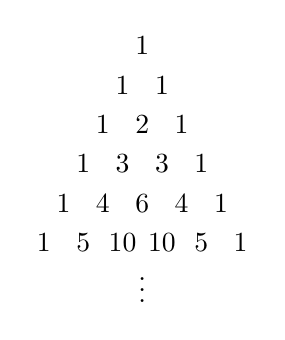
\begin{tikzpicture}[xscale=0.25,yscale=.5]
      \node (00) at ( 0, 0) {$1$};
      \node (10) at (-1,-1) {$1$};
      \node (11) at ( 1,-1) {$1$};
      \node (20) at (-2,-2) {$1$};
      \node (21) at ( 0,-2) {$2$};
      \node (22) at ( 2,-2) {$1$};
      \node (30) at (-3,-3) {$1$};
      \node (31) at (-1,-3) {$3$};
      \node (32) at ( 1,-3) {$3$};
      \node (33) at ( 3,-3) {$1$};
      \node (40) at (-4,-4) {$1$};
      \node (41) at (-2,-4) {$4$};
      \node (42) at ( 0,-4) {$6$};
      \node (43) at ( 2,-4) {$4$};
      \node (44) at ( 4,-4) {$1$};
      \node (50) at (-5,-5) {$1$};
      \node (51) at (-3,-5) {$5$};
      \node (52) at (-1,-5) {$10$};
      \node (53) at ( 1,-5) {$10$};
      \node (54) at ( 3,-5) {$5$};
      \node (55) at ( 5,-5) {$1$};
      \node (d1) at ( 0,-6) {$\vdots$};
    \end{tikzpicture}\\
    \noindent where each number is the sum of the two above, \eg $\binom42 = 6$.}
  \[
    \binom nk \defeq \frac{n!}{k!(n-k)!}.
  \]
  Find a formula for the number of $k$-cycle permutations of $A$
  using factorials and/or binomial coefficients.
\end{xca}

\section{The \texorpdfstring{$m$\th}{mᵗʰ} root:
  \coverings over the components of $\Cyc$}

Recall the equivalence $c : \Sc \we \Cyc_0$ of \cref{def:S1toC}
between the circle and the type of infinite cycles.
Here we set $\Cyc_0 \defeq \InfCyc$.

In this section, we reinterpret the degree $m$ function $\dg{m}$
as a map of infinite cycles. In fact it makes sense as a map on all cycles,
and we'll use it to begin the classification
of the connected \coverings on the components $\Cyc_n$,
of $\Cyc$, determined by the standard $n$-cycles, for positive integers $n$.
That's why it's instructive to rephrase connected \coverings over $\Sc$
in terms of cycles,
even though they could just be transported along the identity $\etop c:\Sc=\Cyc_0$ corresponding to $c$.

Before we do the degree $m$ maps, let's note that the
universal \covering over $\Cyc_0$ is represented by the constant function
$\cst{\pt_0}:\bn 1\to\Cyc_0$, sending the unique element
of $\bn 1$ to $\pt_0\defeq(\zet,\zs):\Cyc_0$, the standard infinite cycle.\footnote{%
  In light of \cref{lem:IdCisZet} we see that the fiber
  of this universal covering over $(X,t):\Cyc_0$ is (equivalent to) $X$ itself
  -- that's certainly a universal set associated to the
  infinite cycle $(X,t)$!}

For the rest of this section, we fix some positive $m:\NN$.
We now give a description of
the $m$-fold \covering over the circle in terms of cycles.

We proceed as follows.
First we present the answer, a \covering we call $\cdg{m}:\Cyc_0\to\Cyc_0$,
and then we prove that $\dg{m}:\Sc\to\Sc$ and $\cdg{m}:\Cyc_0\to\Cyc_0$
correspond to each other (and to $\pow{m}:\tilde R_m\to\Sc$)
under the equivalence $c:\Sc\we\Cyc_0$.

What should we require of $\cdg{m}(X,t)$ for $(X,t):\Cyc_0$?
Well, $\dg{m}:\Sc\to\Sc$ sends $\base$ to $\base$ and $\Sloop$ to $\Sloop^m$;
only the $\Sloop^k$ where $k$ is a multiple of $k$ is in the image of $\dg{m}$.
So we have to find an infinite cycle $(Y,u)$ with ``$u^m$ corresponding to $t$''.
We achieve this by ``streching'' $X$:
Let $Y$ be $m$ copies of $X$ and let $u$ jump idly from one copy to another except every $m$\th time when $u$ also is allowed to use $t$.
This is illustrated in \cref{fig:root} with the shift by $t$ being
vertical and the movement from copy to copy going around a circle.
\begin{marginfigure}
  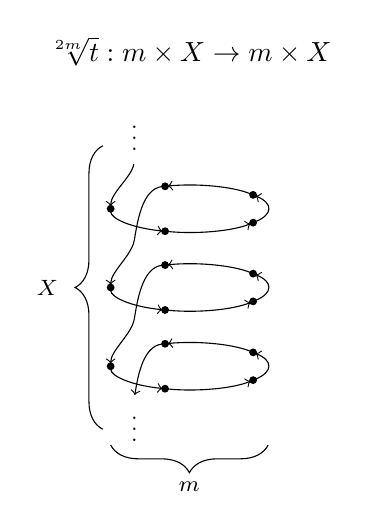
\begin{tikzpicture}
    \node (A) at (0,4) {$\sqrt[\uproot{2}m]t:{\bn m\times X}\to{\bn m\times X}$};
    \foreach \y in {0,1,2}
    { \begin{scope}[shift={(0,\y)}]
        \foreach \x in {0,...,4}
        { \node[fill,circle,inner sep=1pt] at (180+72*\x:1 and .3) {}; }
        \foreach \x in {0,...,3}
        { \draw[->,shorten <=1pt,shorten >=1pt]
          (180+72*\x:1 and .3) arc(180+72*\x:252+72*\x:1 and .3); }
      \end{scope} }
    \foreach \y in {1,2}
    { \begin{scope}[shift={(0,\y)}]
        \draw[->,shorten <=1pt,shorten >=1pt] (108:1 and .3)
        .. controls ++( 5:-.3) and ++(80:.2) .. (-.7,-.4)
        .. controls ++(80:-.2) and ++(90:.2) .. (-1,-1);
      \end{scope} }
    \draw[->,shorten <=1pt,shorten >=1pt] (108:1 and .3)
    .. controls ++( 5:-.3) and ++(80:.2) .. (-.7,-.4);
    \node (dz) at (-.7,-.7) {\footnotesize$\vdots$};
    \begin{scope}[shift={(0,3)}]
      \draw[->,shorten <=1pt,shorten >=1pt] (-.7,-.4)
      .. controls ++(80:-.2) and ++(90:.2) .. (-1,-1);
      \node (da) at (-.7,0) {\footnotesize$\vdots$};
    \end{scope}
    \draw [decorate,decoration={brace,amplitude=10pt}]
    (-1.1,-.8) -- (-1.1,2.8) node [black,midway,xshift=-20pt] {\footnotesize $X$};
    \draw [decorate,decoration={brace,amplitude=10pt}]
    (1,-1) -- (-1,-1) node [black,midway,yshift=-15pt] {\footnotesize $\bn{m}$};
  \end{tikzpicture}
  \caption{The $m$\th root $\sqrt[\uproot{2}m]t$
    of a function $t: X\to X$,
    here illustrated in the case $m=5$.}\label{fig:root}
\end{marginfigure}

\begin{construction}\label{con:root}
  For any type $X$ and $t:X\to X$, we define the $m$\th \emph{root}
  \[
    {\textstyle\sqrt[\uproot{2}m]t} : {\bn m\times X} \to {\bn m\times X}.
  \]
\end{construction}
\begin{implementation}{con:root}
  We set
  \[
    {\textstyle\sqrt[\uproot{2}m]t}(k,x)\defeq
    \begin{cases}
      (k+1,x)& \text{for $k<m-1$ and}\\
      (0,t(x))& \text{for $k=m-1$}.
    \end{cases}
  \]
\par \vspace{-1.5\baselineskip}
\qedhere
\end{implementation}
Only one $m$\th of the time does $\sqrt[\uproot{2}m]t$ use $t:X\to X$,
the rest of the time it applies the successor in $\bn m$.
Indeed, iterating $\sqrt[\uproot{2}m]t$
we get $(\sqrt[\uproot{2}m]t)^m(k,x)=(k,t(x))$;
hence the term ``$m$\th root'' is apt.

\begin{definition}
  The \emph{formal $m$\th root function} is defined by:
  \[
    \cdg{m}:\sum_{X:\UU}(X\to X)\to\sum_{X:\UU}(X\to X),\qquad
    \cdg{m}(X,t)\defeq(\bn m\times X,{\textstyle\sqrt[\uproot{2}m]t}).\qedhere
  \]
\end{definition}
\noindent We use $\rho$ for ``root'' to denote this incarnation
of the degree $m$ function.

\begin{lemma}\label{lem:root-pres-equiv}
  If $t:X\to X$ is an equivalence,
  then so is $\sqrt[\uproot{2}m]t : \bn m\times X \to \bn m\times X$.
\end{lemma}
\begin{proof}
  On one hand, an element in  $(\sqrt[\uproot{2}m]t)(\ell,y) = (0,x)$ consists
  of the assertion that  $\ell=m-1$ and an element in $t(y)=x$,
  so  $(\sqrt[\uproot{2}m]t)^{-1}(0,x)$ is equivalent
  to $t^{-1}(x)$, which is contractible if $t$ is an equivalence.

  On the other, if $k:\bn m$ is not $0$,
  then an element in $(\sqrt[\uproot{2}m]t)(\ell,y)=(k,x)$
  consists of the assertion that $\ell+1=k$ and an element in $y=x$,
  and so $(\sqrt[\uproot{2}m]t)^{-1}(k,x)$ is equivalent
  to the contractible type $\sum_{y:X}y=x$.\marginnote{%
    Of course, it's also quite easy to write down an inverse
    of $\sqrt[\uproot{2}m]{t}$ given an inverse of $t$.}
\end{proof}

\begin{lemma}
  If $(X,t)$ is a cycle, then so is $\cdg{m}(X,t)$.
\end{lemma}
\begin{proof}
  Clearly, $\bn m\times X$ is \nonempty if $X$ is.
  And we already know $\sqrt[\uproot{2}m]{t}$ is an equivalence if $t$ is.

  Suppose $(k,x),(k',x'):\bn m\times X$.
  We need to show the proposition that there exists $n:\zet$
  with $(k',x') = \bigl(\sqrt[\uproot{2}m]t\bigr)^n(k,x)$.
  Let $n:\zet$ be such that $x' = t^n(x)$.
  Then $(\sqrt[\uproot{2}m]t)^{nm}(k,x) = (k,t^n(x)) = (k,x')$,
  so if $k=k'$ we're done.
  Assume $k<k'$. Then $(\sqrt[\uproot{2}m]t)^{k'-k}(k,x') = (k',x')$,
  so $(\sqrt[\uproot{2}m]t)^{nm+k'-k}(k,x) = (k',x')$, as desired.
  The case $k>k'$ is similar.
\end{proof}

The question now arises: how does $\cdg{m}$ act on the components of $\Cyc$,
and what can we say about the preimages $\cdg{m}^{-1}(X,t)$
for an arbitrary cycle $(X,t)$?

The first part is easy, since the product of $\bn m$ with an $n$-element set
is an $mn$-element set. We set $\pt_n \defeq (\bn n,\zs) : \Cyc_n$.
\begin{lemma}
  The degree $m$ function restricts to give pointed maps
  \[
    \cdg{m} : \Cyc_n \ptdto \Cyc_{mn} \quad\text{and}\quad
    \cdg{m} : \Cyc_0 \ptdto \Cyc_0.
  \]
\end{lemma}
\begin{proof}
  Note\marginnote{%
    In terms of iterated addition, we have
    $\varphi(k,r) = (z \mapsto z+m)^r(k)$.}
  that the function $\varphi : (\bn m\times \zet) \to \zet$
  given by $\varphi(k,r)=k+mr$ is an equivalence,
  with inverse given by Euclidean division by $m$.
  Moreover, we have ${\varphi\!\sqrt[\uproot{2}m]\zs} = {\zs\varphi}$, since
  \[
    \varphi\bigl(\!\sqrt[\uproot{2}m]\zs(k,r)\bigr)
    = k+1+mr = \zs(\varphi(k,r))
    \quad\text{for all $(k,r):\bn m\times \zet$}.
  \]
  This shows that $\varphi$ gives an identification of infinite cycles
  $(\bn m\times\zet, \sqrt[\uproot{2}m]\zs) = (\zet,\zs)$,
  and hence the $m$\th root construction maps the component $\Cyc_0$ to itself.

  Analogously, we can restrict $\varphi$ to
  an equivalence $\bn m \times \bn n \we \sum_{k:\NN}(k<mn)$,
  and get an identification of cycles $\cdg{m}(\pt_n) = \pt_{mn}$,
  showing that $\cdg{m}$ maps the component $\Cyc_n$ to the component $\Cyc_{mn}$.
\end{proof}

We now analyze how $\cdg{m}$ acts on paths.
Let $\pathpair{\etop{e}}{!}:(X,t)=(X',t')$.
Since $\cdg{m}$ maps first components $X$ to $\bn m\times X$, we get that
the first projection of $\ap{\cdg{m}}\pathpair{\etop{e}}{!}$ is
$\overetop{\id\times e} : (\bn m\times X) = (\bn m\times X')$.
We are particularly interested in the case of the loops,
that is, $\pathpair{\etop{e}}{!}:(X,t)=(X,t)$.
We calculate $(\id\times e)(k,x) = (k,e(x))$,
which by the property of the $m$\th root is equal to $(\sqrt[\uproot{2}m]e)^m(k,x)$.
In particular, if we take $e\defeq t^{-1}$,
then we get $(\id\times t^{-1}) = (\sqrt[\uproot{2}m]{t^{-1}})^m$, which means that
$\ap{\cdg{m}}\pathpair{\etop{t}^{-1}}{!}$ is indeed the $m$\th power of a
generating loop at the image cycle $\cdg{m}(X,t)$.
In particular, this holds for the standard infinite cycle $(\zet,\zs):\Cyc_0$
and the standard $n$-cycle $(\bn n,\zs):\Cyc_n$.

Why does $\cdg{m}:\Cyc_0\to\Cyc_0$
correspond to the $m$-fold \covering we defined in \cref{def:mfoldS1cover}?
This is encapsulated by the fact that under the equivalence $c:\Sc\to C$, the two $m$-fold covers agree in the sense that the two functions given as composites in
\[
  \begin{tikzcd}
    \Sc\ar[r,"c"]\ar[d,"\dg{m}"'] & \Cyc_0\ar[d,"\cdg{m}"] \\
    \Sc\ar[r,"c"] & \Cyc_0
  \end{tikzcd}
\]
are equal; we need an element in
\[
  \cdg{m}c=_{\Sc\to\Cyc_0}c\,\dg{m}.
\]
Under the equivalence
\[
  \ev_{\Cyc_0}:(\Sc\to\Cyc_0)\we \sum_{(X,t):\Cyc_0}\bigl((X,t)=(X,t)\bigr)
\]
of \cref{lem:freeloopspace},
the composite $c\,\dg{m}$ is given by $\bigl((\zet,\zs),\zs^{-m}\bigr)$
and the composite $\cdg{m}c$ is given by
$\bigl((\bn m\times\zet,\sqrt[\uproot{2}m]{\zs}),\id\times\zs^{-1}\bigr)$:
we must produce an element in
\[
  \Bigl((\bn m\times\zet,\sqrt[\uproot{2}m]{\zs}),\id\times\zs^{-1}\Bigr)
  = \bigl((\zet,\zs),\zs^{-m}\bigr).
\]
Consider the equivalence  $\varphi: (\bn m\times \zet)\to\zet$ with $\varphi(k,n)=k+mn$ discussed above.
Transport of $\sqrt[\uproot{2}m]\zs$ along $\varphi$ is exactly $\zs$.
(I.e., $\varphi\!\sqrt[\uproot{2}m]\zs=\zs\varphi$;
note the way we formulate this so that we don't need to talk about the inverse of $\varphi$\footnote{%
  Of course, the inverse of $\varphi$ maps $z:\zet$ to the remainder and the integer quotient of $z$ under Euclidean division by $m$, cf.~\cref{lem:euclid-div}.}.)
Likewise, transport of $\id\times\zs^{-1}$ along $\varphi$ is $\zs^{-m}$,
so that $\varphi$ lifts to an element in
$\bigl((\bn m\times\zet,\sqrt[\uproot{2}m]{\zs}), \id\times\zs^{-1}\bigr)
= \bigl((\zet,\zs),\zs^{-m}\bigr)$.

\begin{xca}\label{xca:pointed-maps-circle}
Verify $\cdg{m}c=_{\Sc\ptdto\Cyc_0}c\,\dg{m}$ in case all maps are taken to be pointed.
\end{xca}

So we know that the fiber of $\cdg{m}$ at an infinite cycle $(X,t)$
is an $m$-element set. In fact, we can identify this set as
$X/m \defeq X/\sim_m$ where $\sim_m$ is the equivalence relation that
identifies points that are a distance $mr$ apart, for some $r:\zet$.
Formally, let $x\sim_m x'$ if and only if $\exists_{r:\zet}(x'=t^{mr}(x))$.
(Such an $r$ is unique if it exists.)
Indeed, the fiber is
\[
  \sum_{(Y,u):\Cyc_0}\bigl((X,t) = (\bn m\times Y, \sqrt[\uproot{2}m]{u})\bigr).
\]
The equivalence is obtained by sending an equivalence class $Y$ of $X/m$ to
the corresponding infinite cycle $(Y,u^m)$ together with the
natural identification $(X,t) = (\bn m\times Y, \sqrt[\uproot{2}m]{u^m})$.
See \cref{thm:fiber-cdg} below for a careful proof of a more general statement.

The reader will no doubt have noticed that $X/m$ is a \emph{finite cycle}.
We'll return to the significance of this below in~\cref{sec:higher-images}.

Our next step is to identify the fiber of $\cdg{m}$ over a general cycle $(X,t)$.
Classically, the remaining cases are those of finite $n$-cycles,
but it's illuminating to be a bit more general.
Note that the equivalence relation $\sim_m$ defined above for an infinite cycle
makes sense for all cycles.

\begin{lemma}\label{lem:sum-cycle-point-contr}
  For any order $d:\Order$, the type $\sum_{(X,t):\Cyc_d}X$ is contractible,
  where $\Cyc_d$ denotes the component of $\Cyc$ consisting
  of cycles of order $d$.
\end{lemma}
\begin{proof}
  This is relatively straight-forward from \cref{lem:IdCycle}.
  The type in question is nonempty since all cycles have a nonempty underlying set,
  so it suffices to prove the type is a proposition.
  So let $(X,t),(X',t')$ be cycles of order $o$, and take $x:X$ and $x':X$.
  An identification $((X,t),x) = ((X',t'),x')$ is given by an equivalence of
  cycles $e : (X,t)=(X',t')$ with $e(x)=x'$.
  But evaluation at $x$ induces an equivalence
  $\bigl((X,t)=(X',t')\bigr) \simeq X'$,
  so there exists a unique $e$ with $e(x)=x'$.
\end{proof}
\begin{lemma}\label{lem:m-root-id}
  For any cycle $(X,t)$, if $(\sqrt[\uproot{2}m]{t})^n = \id$,
  then $m$ divides $n$, \ie $n=mq$ for some $q:\zet$, and $t^q=\id$.
  In other words, $m$ divides the order of $\sqrt[\uproot{2}m]{t}$.
\end{lemma}
This follows simply by looking at the first component,
where $\sqrt[\uproot{2}m]{t}$ acts as the successor operation on $\bn m$.

We're almost ready to identify the fiber of $\cdg{m}$ at a cycle $(X,t)$.
We know from \cref{lem:m-root-id} that the fiber
is \nonempty only if $m$ divides the order of $t$.
A key ingredient for the converse is the following.
\begin{lemma}\label{lem:X-mod-m-chosen}
  Let $(X,t):\Cyc$ be a cycle with a chosen point $x_0:X$
  and with order divisible by $m$.
  Then the map $f : \bn m \to X/m$, $f(k) \defeq [t^k(x_0)]$
  is an equivalence.
\end{lemma}
\begin{proof}
  Fix an equivalence class $V:X/m$ and consider its preimage under $f$,
  $f^{-1}(V) \jdeq \sum_{k:\bn m}(V=[t^k(x_0)])$.
  The contractibility of this type is a proposition, so we may choose
  $x:X$ with $V=[x]$.
  Then $(V=[t^k(x_0)])\equiv([x]=[t^k(x_0)])\equiv(x\sim_m t^k(x_0))$.
  So we need to show that $\sum_{k:\bn m}(x\sim_m t^k(x_0))$ is contractible.
  More simply, we need to show that there is a unique $k$ with $x\sim_m t^k(x_0)$.
  Since $(X,t)$ is a cycle, we may further choose $n:\zet$ with $x=t^n(x_0)$.
  By Euclidean division, write $n=qm+r$ with $q:\zet$, $r:\bn m$.
  Then $x = t^n(x_0) \sim_m t^r(x_0)$, so we have our center.
  Let $k:\bn m$ also satisfy $x\sim_m t^k(x_0)$.
  We need to show the proposition $k=r$.
  But $t^{r-k}(x_0) \sim_m x_0$, so we may take $q:\zet$ with $t^{qm+r-k}(x_0)=x_0$.
  Since $m$ divides the order of $t$, this implies $r=k$, as desired.
\end{proof}
Now we have all the pieces needed to prove the main result.
\begin{theorem}\label{thm:fiber-cdg}
  For \emph{any} cycle $(X,t)$, the preimage $\cdg{m}^{-1}(X,t)$
  is equivalent to $P\times X/m$,
  where $P\defeq (m \mid \ord(t)) \jdeq (H_t \subseteq m\zet)$
  expresses that $m$ divides the order of $t$.
\end{theorem}
\begin{proof}
  We'll use \cref{lem:weq-iso}, and we first define the function
  \[
    g : \cdg{m}^{-1}(X,t) \to P\times X/m,
  \]
  by mapping $(Y,u)$ and an identification of cycles
  $e : (X,t) = (\bn m\times Y,\sqrt[\uproot{2}m]{u})$
  to the proof of $P$ from \cref{lem:m-root-id}
  and the class $V_e\defeq [e^{-1}(0,y)]:X/m$, for any $y:Y$.
  Note that this doesn't depend on $y$, so that \cref{thm:wconstant-elim} applies.
  As a subset of $X$, $V_e=\setof{x:X}{\fst(e(x))=0}$.

  In the other direction, to define the function
  \[
    h : P\times X/m \to \cdg{m}^{-1}(X,t),
  \]
  fix an equivalence class $V:X/m$,
  and assume that $m$ divides the order of $t$.
  Then we have, with a bit of abuse of notation, the cycle $(V,t^m)$,
  where we also write $V$ for the type of elements in $X$ that lie in the class $V$,
  and $t^m$ is the restriction of this power of $t$ to $V$.\footnote{%
    If $x$ lies in $V$, then so does $t^m(x)$.}
  We also need an identification
  $(X,t)=(\bn m\times V,\sqrt[\uproot{2}m]{t^m})$.
  This we define via a map $e : \bn m\times V \to X$, $e(k,x) \defeq t^k(x)$.
  This is an equivalence as long as the orders match.
  So let $n:\zet$, and assume first that $t^n=\id$.
  Then $P$ implies that we may write $n=qm$ for some $q:\zet$,
  so
  \[
    (\sqrt[\uproot{2}m]{t^m})^n
    = (\sqrt[\uproot{2}m]{t^m})^{qm}
    = (\id \times t^m)^q = (\id \times t^{qm}) = \id.
  \]
  Conversely, we know from \cref{lem:m-root-id} again,
  that if $(\sqrt[\uproot{2}m]{t^m})^n=\id$,
  then we may write $n=qm$ for some $q:\zet$,
  and $(t^m)^q=\id$, which by \cref{lem:cycle-order-point-ap}
  implies that $t^n = \id$.

  Straight from these definitions, we see that $g\circ h=\id$.
  We leave to the reader to check that $h\circ g=\id$.
\end{proof}

\section{Higher images}
\label{sec:higher-images}

In this section we take a quick break from characterizing the connected \coverings
of $\Cyc_n$ for finite orders $n$ in order to make good on our earlier promise
to say something about the fact that the fiber of $\cdg{m}$, $X/m$, at a cycle $(X,t)$
of order divisible by $m$, itself carries a cycle structure.
This involves the notion of $0$-image of a map, but we might as well introduce the general
notion of $n$-image while we're at it.

Recall from \cref{def:prop-image} the propositional image of a map $f : A \to B$,
  \[
    \im(f) \jdeq \sum_{y:B}\exists_{x:A}(y \eqto f\,x)
           \jdeq \sum_{y:B}\Trunc{\sum_{x:A}(y \eqto f\,x)}
           \jdeq \sum_{y:B}\Trunc{\inv f (y)}.
  \]
We now generalize the propositional image
to higher images, replacing the propositional
truncation involved in the definition by $n$-truncation.

Recall furthermore the image factorization from \cref{xca:unique-fact-image}:
  \[
    \begin{tikzcd}
      A \ar[rr,"f"]\ar[dr,"p"'] & & B \\
      & \im(f)\ar[ur,"i"'] &
    \end{tikzcd}
  \]
Here $p$ is surjective and $i$ is injective, and any such factorization is equivalent to this one. Both surjectivity
(\cref{def:surjection}) and injectivity (\cref{def:injection})
rely on the notion of proposition: all fibers of $p$ are nonempty
and all fibers of $i$ are propositions.

The uniqueness of the factorization $f=ip$ can be visualized
in terms of the two diagonals of the diamond below:
for any surjection $g$ and injection $h$ such that $f=hg$,
that is, the diagram below on the left commutes,
one can construct a (unique) equivalence $e$ such that
the diagram on the right commutes.

\begin{equation}\label{eqn:image-univ-prop}
    \begin{tikzcd}
      & X \ar[dr,"h"] & & & X \ar[dr,"h"] &\\
      A \ar[rr,"f"]\ar[dr,"p"'] \ar[ur,"g"]& & B
&
      A \ar[dr,"p"'] \ar[ur,"g"]& & B  \\
      & \im(f)\ar[ur,"i"'] & & & \im(f)\ar[ur,"i"']\ar[uu, dotted, "e"] &
    \end{tikzcd}
\end{equation}

The existence of a unique equivalence $e$ as above is called the
\emph{universal property of the propositional image}.
Uniqueness of $e$ above also follows from the following two exercises.

\begin{xca}\label{xca:cancel-injection}
Let $A,B,X$ be types and $i:A\to B$ an injection.
Let $i\blank : (X\to A) \to (X\to B)$ be postcomposition with $i$.
Show that $\ap{i\blank}: (f = g) \to (if = ig)$ is an equivalence,
for any $f,g: X\to A$.
\end{xca}
\begin{xca}\label{xca:cancel-surjection}
Let $A,B,Y$ be types and $p:A\to B$ be a surjection.
Let $\blank p : (B\to Y) \to (A\to Y)$ be precomposition with $p$.
Show that $\ap{\blank p}: (f = g) \to (fp = gp)$ is an equivalence,
for any $f,g: B\to Y$.
\end{xca}

We will now define higher images and generalize the notions
of injection and surjection such that a similar
universal property of higher images can be proved.

\begin{definition}\label{def:n-image}
  Let $A,B$ be types and let $f : A \to B$. We define the $n$-\emph{image} of $f$ as
  \glossary(iman){$\protect\im_n(f)$}{the $\protect n$-image of $\protect f$}
  \[
    \im_n(f) \defeq \sum_{b:B}\Trunc{\inv f (b)}_n.\qedhere
  \]
\end{definition}

Observe that $\im_{-1}(f) \jdeq \im(f)$.

\begin{definition}\label{def:n-connected}
  A type $A$ is called $n$-\emph{connected}\index{type!$n$-connected}
  if its truncation $\Trunc A _ n$ is contractible.

  A function $f : A \to B$ is called $n$-\emph{connected}\index{function!$n$-connected}
  if the fiber $\inv f (b)$ is $n$-connected, for each $b:B$.
\end{definition}

Thus, any type is $(-2)$-connected, since its $(-2)$-truncation is contractible.
Moreover, the $(-1)$-connected types are precisely the nonempty ones,
and the $0$-connected types are those we have called connected in \cref{def:connected}.

\begin{definition}\label{def:n-truncated}
  A function $f : A \to B$ is called $n$-\emph{truncated}\index{function!$n$-truncated}
  if the fiber $\inv f (b)$ is an $n$-type, for each $b:B$.
\end{definition}

One may verify now that the $(-1)$-connected functions are the surjections, and
the $(-1)$-truncated functions are the injections.

There is a \emph{factorization} $f = i p$ of a map $f : A \to B$ through its $n$-image,
where $p$ is defined by setting $p(a)\defeq (f(a),\trunc{(a,\refl{f(a)})}_n)$,
and where $i$ is defined by setting $i\defeq\fst$, as in the following diagram.

\begin{equation}\label{eqn:n-image-factorization}
    \begin{tikzcd}
      A \ar[rr,"f"]\ar[dr,"p"'] & & B \\
      & \im_n(f)\ar[ur,"i"'] &
    \end{tikzcd}
\end{equation}

The map $i$ is $n$-truncated, because, for any $b:B$, the fiber $\inv i (b)$ is equivalent to $\Trunc{\inv f (b)}_n$.
Furthermore, by \cref{lem:sum-of-fibers} and the following lemma, $p$ is $n$-connected.

\begin{lemma}\label{lem:trunc-n-connected}
For every type $A$, the constructor $\trunc{\blank}_n : A\to \Trunc{A}_n$
is $n$-connected.
\end{lemma}
\begin{proof}
We have to prove that the $n$-truncation of each fiber of $\trunc{\blank}_n$
is contractible. We start by defining a function
$c:\prod_{x:\Trunc{A}_n} \Trunc{\inv{\trunc{x}}_n}_n$ producing the centers.
Since $c$ takes values in $n$-types, we can define $c$ by
$n$-truncation elimination by setting
$c(\trunc{a}_n) \defeq \trunc{(a,\refl{\trunc{a}_n})}_n$.

The next step is to construct an element of
$\prod_{x:\Trunc{A}_n} \prod_{y:\Trunc{\inv{\trunc{x}}_n}_n} (c(x)=y)$.
Since the identity $c(x)=y$ is an $(n-1)$-type, it suffices to give an element of
$\prod_{x:\Trunc{A}_n} \prod_{z:\inv{\trunc{x}}_n} (c(x)=\trunc{z}_n)$.
Since fibers are sum types,  it suffices to give an element of
$\prod_{x:\Trunc{A}_n} \prod_{a:A} \prod_{p: x=\trunc{a}_n} (c(x)=\trunc{(a,p)}_n)$.
After swapping the first two products, the identity reduces by path induction
to $c(\trunc{a}_n)=\trunc{(a,\refl{\trunc{a}_n})}_n$, for which we can use
the reflexivity path.
\end{proof}

\begin{construction}\label{con:fibcomp=fibfib}
  Let $g:A\to X$ and $h: X\to B$, and let
$\tilde{g}:A\to \sum_{b:B}\inv h (b)$ be the composition of $g$
with the canonical equivalence $X\to \sum_{b:B}\inv h (b)$ from \cref{lem:sum-of-fibers}.
Thus $\tilde{g}(a)\jdeq (h(g(a)),g(a),\refl{h(g(a))})$ for each $a:A$,
and we have the following commutative diagram:
  \[
    \begin{tikzcd}
      A \ar[r,"g"] \ar[dr,"\tilde{g}"'] & X \ar[r,"h"] \ar[d, eqr] & B \\
      & \sum_{b:B}\inv h (b) \ar[ur,"\fst"'] &
    \end{tikzcd}
  \]
Then we have equivalences $e(b) : \inv {(hg)} (b) \equivto \sum_{y:\inv h (b)} \inv {\tilde{g}}(b,y)$
for all $b:B$.
\end{construction}
\begin{implementation}{con:fibcomp=fibfib}
Let, for each $b:B$, $e(b)$ map any pair $(a,p):\inv {(hg)} (b)$ to
$((g(a),p),(a,q))$. Here $q$ is of type $(b,g(a),p) = (h(g(a)),g(a),\refl{h(g(a))})$
and is given componentwise by $p: b=h(g(a))$, $\refl{g(a)}$, and by the
easy path over $p$ from $p$ to $\refl{h(g(a))}$ in the identity type family $\blank=h(g(a))$.
This construction uses \cref{def:pairtopath}, \cref{def:pathover-trp},
and \cref{xca:trp-in-a/x=b/x}\ref{trp-in-x=a}.
\end{implementation}

\begin{xca}\label{xca:fibcomp=fibfib}
Complete the details of \cref{con:fibcomp=fibfib}.
In particular, prove that $e$ is a fiberwise equivalence.
Alternatively, construct your own $e$ by using \cref{cor:contract-away} (twice!).
\end{xca}

\begin{xca}\label{xca:pullout-base-type}
Let $X$ be an $n$-type and let $Y(x)$ be a type for all $x:X$.
Construct canonical equivalences
$\Trunc{\sum_{x:X} Y(x)}_n \to \sum_{x:X} \Trunc{Y(x)}_n$  and
$\Trunc{\prod_{x:X} Y(x)}_n \to \prod_{x:X} \Trunc{Y(x)}_n$.
\end{xca}

We shall now show that the $n$-image factorization
of $f:A\to B$ in \cref{eqn:n-image-factorization} is unique.
This result can be visualized in a similar way as we
did in \cref{eqn:image-univ-prop} for $n=-1$,
and is called the \emph{universal property of the $n$-image}.

\begin{marginfigure}
\noindent\begin{tikzcd}
      & X \ar[dr,"h"] & \\
      A \ar[rr,pos=0.7,"f"]\ar[dr,"p"'] \ar[ur,"g"]& & B\\
      & \im_n(f)\ar[ur,"i"']\ar[uu,dotted,pos=0.3, "e"] &
    \end{tikzcd}
\caption{Universal property of the $n$-image.}
\label{fig:n-image-univ-prop}
\end{marginfigure}

\begin{theorem}\label{thm:n-im-univ-prop}
Let conditions be as in \cref{eqn:n-image-factorization}.
For a given type $X$, assume we are given an $n$-connected
function $g:A\to X$ and an $n$-truncated function $h:X\to B$ with $f=hg$.
Then there exists a unique equivalence $e: \im_n(f)\to X$
such that $g=ep$ and $i=he$.
\end{theorem}

\begin{proof}
We have to construct the equivalence $e$ such that the diagram
in \cref{fig:n-image-univ-prop} commutes; uniqueness of $e$
follows from an easy generalization of \cref{xca:cancel-injection}
and the left triangle in \cref{fig:n-image-univ-prop}.
To simplify this construction,
we are going to replace $g$ and $h$ by projection maps.

In view of \cref{con:fibcomp=fibfib}, we may assume without
loss of generality that $X\jdeq \sum_{b:B} P(b)$ for some
family of $n$-types $P(b)$, and $h\jdeq\fst$.

\begin{marginfigure}
  \noindent\begin{tikzcd}[column sep=tiny]
      &\sum\limits_{b:B} P(b)\ar[rd,"\fst"]\\
      \sum\limits_{b:B} R(b)
        \ar[rd,"{(b,y,q)\mapsto(b,\trunc{(y,q)}_n)}"']
        \ar [ru,"{(b,y,q)\mapsto(b,y)}"]
        \ar [rr,pos=0.7,"\fst"]
      &&B\\
      &\sum\limits_{b:B} \Trunc{R(b)}_n
         \ar [ru,"\fst"']
         \ar [uu,dotted,pos=0.3,"e"']
\end{tikzcd}
\caption{Universal property of the $n$-image, reinterpreted.}
\label{fig:n-im-univ-prop-sumB}
\end{marginfigure}

By \cref{lem:sum-of-fibers} we may also assume without
loss of generality that
$A\jdeq\sum_{b:B}\sum_{y:P(b)} Q(b,y)$, where
$Q(b,y) \defeq\inv g (b,y)$ are the fibers of $g$,
which are all $n$-connected by assumption.
Define $R(b)\defeq\sum_{y:P(b)} Q(b,y)$ for all $b:B$.
With $A\jdeq \sum_{b:B} R(b)$, the function $g$
takes the form of the projection map $(b,y,q)\mapsto(b,y)$,
as shown in \cref{fig:n-im-univ-prop-sumB}.
By $f=hg$ we then get that $f$ is the first projection,
with its $n$-image equivalent to $\sum_{b:B} \Trunc{R(b)}_n$.
The $n$-connected map $p$ then takes the form
$(b,y,q)\mapsto(b,\trunc{(y,q)}_n)$ as shown in
\cref{fig:n-im-univ-prop-sumB}.

Since $B=\sum_{b:B}\bn{1}$, each type in \cref{fig:n-im-univ-prop-sumB}
can be considered to be the sum of a type family parametrized by $b:B$.
For constructing the equivalence $e$ that makes
\cref{fig:n-im-univ-prop-sumB} commute, it suffices to
construct for each $b:B$ the equivalence $e_b$ such that
\cref{fig:n-im-univ-prop-b:B} commutes.
Then we obtain $e$ as desired by summing over $B$, that is,
by putting $e(b,z) \defeq (b,e_b(z))$ for all $b:B$ and $z:\Trunc{R(b)}_n$.

\begin{marginfigure}
  \noindent\begin{tikzcd}
      &P(b)\ar[rd]\\
      R(b)
        \ar[rd,"{\trunc{\blank}_n}"']
        \ar [ru,"{\fst}"]
      &&\bn{1}\\
      &\Trunc{R(b)}_n
         \ar [ru]
         \ar [uu,dotted,"e_b"']
\end{tikzcd}
\caption{Taking summands for $b:B$ in \cref{fig:n-im-univ-prop-sumB}.}
\label{fig:n-im-univ-prop-b:B}
\end{marginfigure}

Now let $b:B$. We have $\Trunc{R(b)}_n \jdeq \Trunc{\sum_{y:P(b)} Q(b,y)}_n$.
By \cref{xca:pullout-base-type}, since $P(b)$ is an $n$-type by assumption,
we have the canonical equivalence
$\Trunc{\sum_{y:P(b)} Q(b,y)}_n\to\sum_{y:P(b)}\Trunc{Q(b,y)}_n$
defined by mapping $\trunc{(y,q)}_n$ to $(y,\trunc{q}_n)$.
For each $y:P(b)$, since $Q(y,b)$ is by assumption $n$-connected,
so that $\Trunc{Q(b,y)}_n = \bn{1}$,
we also have the canonical equivalence $\fst: \sum_{y:P(b)}\Trunc{Q(b,y)}_n \to P(b)$.
The composite of these two equivalences is $e_b$. Regarding the commutation
of \cref{fig:n-im-univ-prop-b:B}, we have $e_b \trunc{\blank}_n \jdeq \fst$
for the left triangle, and the right triangle commutes trivially.

An alternative proof of the uniqueness of $e$ can be obtained
by using the right triangle in \cref{fig:n-im-univ-prop-sumB}.
This reduces the uniqueness of $e$ to the uniqueness of $e_b$
for each $b:B$. The latter follows from the universal property
of $n$-truncation and the left triangle in \cref{fig:n-im-univ-prop-b:B}.
\end{proof}

As an application, we consider the fibers of $m$\th root map
$\cdg{m}$. On infinite cycles, this is equivalent to the degree $m$ map
of the circle by~\cref{xca:pointed-maps-circle}, so we have a map
$\blank/m : \Cyc_0 \to \Set$, which we can identify with the family
$R_m : \Sc \to \Set$ (\cref{def:RmtoS1})
after precomposition with the equivalence
$c : \Sc \to \Cyc_0$ from~\cref{thm:S1bysymmetries}.
For every infinite cycle $(X,t)$, the set $X/m$ has $m$ elements,
so the $(-1)$-image is $\FinSet_m$, the groupoid of $m$-element sets
(\cref{def:groupoidFin}).
But what is the $0$-image?

\begin{theorem}\label{thm:image-Z-to-Cm}
  The $0$-image factorization of the map $\blank/m : \Cyc_0 \to \Set$
  is the composition $p\circ q$, where $q : \Cyc_0 \to \Cyc_m$
  sends the infinite cycle $(X,t)$ to the $m$-cycle $(X/m,\bar t)$,
  where $\bar t : X/m \to X/m$ maps $[x]$ to $[t(x)]$,
  and $p:\Cyc_m\to\Set$ sends an $m$-cycle to its underlying set.
\end{theorem}

\begin{proof}
  We need to check that $q$ is $0$-connected
  and that $p$ is $0$-truncated.

  The latter is direct, since the preimage of $p$ at an $m$-element set $Y$
  is the set of functions $u : Y \to Y$ that make $Y$ into an $m$-cycle.

  To show that $q$ is $0$-connected,
  it suffices to consider the fiber at the standard $m$-cycle $(\bn m,\zs)$.
  We'll show that this fiber is equivalent to $\Cyc_0$ itself, which is indeed $0$-connected.
  The mediating map is induced by our old friend $\cdg{m}$.
  Indeed, define $\varphi : \Cyc_0 \to q^{-1}(\bn m,\zs)$
  by $\varphi(X,t)\defis(\cdg{m}(X,t), r)$,
  where $r$ is the canonical equivalence $(\bn m\times X)/m \equivto \bn m$.
  The inverse of $\varphi$, $\psi$, sends a pair $((Y,u), r)$,
  with $(Y,u):\Cyc_0$ and $r : Y/m \equivto \bn m$
  to $(r^{-1}(0), u^m)$.
\end{proof}

\begin{xca}
  Complete the proof by verifying that $\varphi$ and $\psi$ are indeed mutually inverse.
\end{xca}

The theorem and its proof in fact generalize to all orders.

\begin{xca}\label{xca:image-Cmd-to-Cm}
  Let $d$ be any order and consider the fiber of $\cdg{m}$ on the component
  $\Cyc_{md}$, $\blank/m : \Cyc_{md} \to \Set$.
  Show that the $0$-image factorization of this goes via $\Cyc_m$ by
  lifting $\blank/m$ to $q : \Cyc_{md} \to \Cyc_m$.
  In particular, show that the preimage of $q$ at the standard $m$-cycle
  is equivalent to $\Cyc_d$.
\end{xca}

\section{Universal property of $\Cyc_n$}
\label{sec:universal-property-cyc-n}

This section is devoted to showing that maps out of $\Cyc_n$ into a groupoid $A$
are equivalently given by the choice of a point together with a symmetry of
order $n$: that is any map $\Cyc_n \to A$ is fully determined by a point $a$ together with a symmetry $\sigma:a\eqto a$ such that
$\sigma^n=\refl a$.\footnote{Notice that this is a less general result than the universal property of the circle, or equivalently, the case $n=0$, where we don't need to assume that $A$ is a groupoid.}

Recall that $\Cyc_n$ contains the point $\pt_n \defequi (\bn n, \zs)$,
\ie the standard $n$-cycle. This
point has a symmetry $\sigma_n \defequi (\inv\zs, !)$ whose second projection is a
proof that $\zs\inv\zs = \inv\zs\zs$.
%
Recall also from \cref{cor:id-m-cycle} that all elements of $\pt_n = \pt_n$ are
of the form $\sigma_n^i$ for $i=0,\dots,n-1$.

Given a groupoid $A$, and a map $f :
\Cyc_n \to A$, one can consider $f(\pt_n):A$ and $\ap f (\sigma_n): f(\pt_n) =
f(\pt_n)$. The equation $\refl {\pt_n} = \sigma_n^n$ in
$\Cyc_n$ is mapped by $f$ to a proof of $\refl {f(\pt_n)} =
\ap f(\sigma_n)^n$. Hence, the following map is well-defined:
\begin{displaymath}
  \ev_{n,A} : (\Cyc_n \to A) \to \sum_{a:A}\sum_{\sigma:a\eqto a}\refl a = \sigma^n,\quad
  f \mapsto (f(\pt_n), \ap f (\sigma_n), !)
\end{displaymath}

\begin{theorem}
  For any groupoid $A$, the map $\ev_{n,A}$ is an equivalence.
  \label{prop:ump-cycn-into-groupoids}
\end{theorem}
\begin{proof}
  Let $a:A$ and $\sigma:a\eqto a$ be such that $\refl a = \sigma^n$ holds.
  We want to prove that the fiber
  \begin{displaymath}
    \sum_{f:\Cyc_n \to A} (a,\sigma, !) \eqto \ev_{n,A}(f)
  \end{displaymath}
  is contractible. Hence we first need to craft a function $f:\Cyc_n \to A$
  together with $p:a\eqto f(\pt_n)$ such that $\ap f (\sigma_n) \cdot p = p
  \cdot \sigma$.

  In order to do so, we will craft a function $f:\Cyc_n \to A$ together with a
  function $\hat p_x: \pt_n \eqto x \to a \eqto f(x)$ for each $x:\Cyc_n$ such that
  $\hat p_x(\blank\sigma_n) = \hat p_x(\blank) \sigma$. By setting $p \jdeq \hat
  p_{\pt_n}(\refl {\pt_n})$, we would have succeeded. Indeed, path induction on
  $\alpha: x \eqto x'$ shows that $\hat p_{x'}(\alpha \blank) = \ap f (\alpha) \hat
  p_x(\blank)$ on one hand, and the hyptohesis on $\hat p$ proves that $\hat
  p_{\pt_n} (\blank) \sigma = \hat p_{\pt_n}(\blank \sigma_n)$ on the other
  hand. This leads to the chain of equations:
  \begin{align*}
    p \sigma &= \hat p_{\pt_n}(\refl {\pt_n}) \sigma
               = \hat p_{\pt_n}(\refl {\pt_n}\sigma_n)
               = \hat p_{\pt_n}(\sigma_n\refl {\pt_n}) \\
             &= \ap f (\sigma_n) \hat p_{\pt_n}(\refl {\pt_n})
               = \ap f (\sigma_n) p
  \end{align*}

  It remains to craft the promised $f$ and $\hat p$. For each $x:\Cyc_n$, consider the type
  \begin{displaymath}
    T(x) \defequi \sum_{b:A}\sum_{\pi: \pt_n \eqto x \to a \eqto b}
    \pi(\blank\sigma_n) = \pi(\blank) \sigma
  \end{displaymath}
  We claim that $T(x)$ is contractible. To prove this proposition for $x$
  ranging over the connected type $\Cyc_n$, it is enough to only prove it for
  $x \jdeq \pt_n$. However, as $i \mapsto \sigma_n^i$ provides an equivalence
  $\bn n \to (\pt_n = \pt_n)$, we get:
  \begin{displaymath}
    T(\pt_n) \weq \sum_{b:A}\sum_{\pi: \bn n \to a \eqto b} \pi(\blank + 1) = \pi(\blank)\sigma
  \end{displaymath}
  Now, note that $\pi:\bn n \to a\eqto b$ such that $\pi(\blank +1) = \pi(\blank)
  \sigma$ is entirely determined by $\pi(0)$, as then $\pi(i) = \pi(0)\sigma^i$
  for all $i:\bn n$. Moreover, an element $q$ in $a\eqto b$ defines a function
  $\pi_q:i \mapsto q\sigma^i$ which satisfies the equation $\pi_q( \blank +1) =
  \pi_q(\blank)q$. In other words, we have an equivalence:
  \begin{displaymath}
    \left( \sum_{\pi:\bn n \to {a\eqto b}} \pi(\blank +1) = \pi(\blank )\sigma \right)
    \equivto
    (a \eqto b), \quad
    (\pi, !) \mapsto \pi(0).
  \end{displaymath}
  Hence, we can simplify further $T(\pt_n)$:
  \begin{displaymath}
    T(\pt_n) \weq \left(\sum_{b:A} a \eqto b\right) \weq 1
  \end{displaymath}
  We then get $f(x)$ by selecting a center of contraction for each $x:\Cyc_n$, and
  the function $\hat p_x$ is then defined as the first projection of the second
  component of this center of contraction.
  %
  \marginnote{The construction of $f$ is really an ad hoc version of the delooping of the abstract group morphism $\sigma_n^i \mapsto \sigma^i$. If we move this section forward, one can rewrite it as such.}


  Finally, we prove that the fiber $\inv{\ev_{n,A}}(a,\sigma,!)$ is a
  proposition. As we just proved that it is inhabited, we would have
  successfully shown that the fiber is contractible. Given two elements
  $(f,p,!)$ and $(f',p',!)$ of the fiber, we want to find a path between the
  two, that is $\chi:\prod_{x:\Cyc_n} f(x) \eqto f'(x)$ such that the following
  commutes:
  \begin{displaymath}
    \begin{tikzcd}
      a \rar[eqr,"p"] \dar[eql,"p'"'] & f(\pt_n) \dlar[eqr,"\chi(\pt_n)"]\\
      f'(\pt_n) &
    \end{tikzcd}
  \end{displaymath}
  Let us denote $U(x)\defequi f(x) \eqto f'(x)$ for $x:\Cyc_n$, and notice that
  these types are sets (as $A$ is a groupoid). The element $\tau\defequi p'\inv
  p : U(\pt_n)$ is peculiar in that  $\trp[U] q (\tau) = \tau$ for all $q:\pt_n\eqto\pt_n$.
  Indeed, we use once
  again that symmetries of $\pt_n$ in $\Cyc_n$ are of the form $\sigma_n^i$ and
  we calculate:
  \begin{displaymath}
    \trp[U] {\sigma_n^i} (\tau) = \ap {f'} (\sigma_n^i) \cdot \tau \cdot \inv{\ap {f}(\sigma_n^i)}
    = p' \sigma^i \inv {p'} \cdot p'\inv p p \sigma^{-i} \inv p = p' \inv p
  \end{displaymath}
  Now it is easy to prove that the following type is contractible:
  \begin{displaymath}
    V(x) \defequi \sum_{\alpha: U(x)} \alpha = \trp[U] \blank (\tau).
  \end{displaymath}
  To do so, we use the connectedness of $\Cyc_n$ and verify the contractibility
  of $V(\pt_n)$ by pointing out that $V(\pt_n)$ is simply the singleton type of
  $\tau$. Now $\chi$ is defined as the function mapping $x$ to the center of
  contraction of $V(x)$. By definition, $\chi(\pt_n) = \tau$ as we wanted.
  %
  \marginnote{The construction of $\chi$ is really an ad hoc version of the following fact: for any $G$-set $X$, the type of fixed points of $X$ is equivalent to the type of sections of $\sum_{z:\BG}X(z) \to \BG$. If we move this section forward, one can rewrite it as such.}
\end{proof}

As a direct corollary, we can classify the connected \coverings of $\Cyc_n$ for finite orders $n$.
Indeed, the corresponding families $S : \Cyc_n \to \Set$ are precisely those cycles $(X,t)$
with $t^n=\id$, \ie whose order divides $n$.
If we restrict to decidable connected \coverings, equivalently, decidable cycles,
these are the usual finite cycles with order dividing $n$.

\section{Getting our cycles in order}
\label{sec:cycles-order}

{\color{casblue} TODO: Exposition and figures

\begin{xca}
  Prove that if $(X,t),(Y,u)$ are cycles, $x_0:X$,
  then the type of maps $f : (X,t) \to (Y,u)$ is equivalent to $P\times Y$,
  where $P\defeq(\ord(u) \mid \ord(t)) \jdeq (H_t \subseteq H_u)$.
\end{xca}

Thus, an order $p$ divides an order $q$ if and only if
there is a map of cycles from a cycle of order $q$
to a cycle of order $p$.
\begin{theorem}
  The partially ordered set $(\Order,|)$ is a lattice
  with least element the finite order $1$
  and greatest element the infinite order, represented by the number $0$,
  and meets and joins given by “gcd” and “lcm”, respectively.
\end{theorem}

subgroups of $\CG_n$: $\CG_k$ where $k | n$,
connected set bundles of $\Cyc_n$.

\subsection{More TODO}

\begin{itemize}
\item Classify connected \coverings over $\Cyc_n$.
\item Universal property of $\Cyc_n$ among groupoids.
\item Bijective proof of $mn = \lcm(m,n)\times\gcd(m,n)$ via the product of cycles.
  Chinese remainder stuff.
\item Somehow sneak in totatives and automorphisms of cyclic groups?
\end{itemize}
}


%%% Local Variables:
%%% mode: latex
%%% TeX-master: "book"
%%% End:

\chapter{Groups}
\label{ch:groups}


An identity type is not just any type:  in the previous sections we have seen that the identity type $a\eqto_Aa$ reflects the ``symmetries'' of an element $a$ in a type $A$.\footnote{%
  Since the symmetries $p : a\eqto_A a$ are paths that start and end
  at the point $a:A$, we also call them \emph{loops} at $a$.\par
  \begin{tikzpicture}
    \draw plot [smooth cycle] coordinates {(0,0) (2.3,0) (2,1.9) (0,2.1)};
    \node[dot,label=left:$a$] (a) at (0.5,0.3) {};
    \node (A) at (2.5,2.1) {$A$};
    \draw[->] (a) .. controls ++(-10:3) and ++(100:2.5) .. node[auto,swap] {$p$} (a);
  \end{tikzpicture}}
Symmetries have special properties.  For instance, you can rotate a square by $90\mathdegree$, and you can reverse that motion by rotating it by $-90\mathdegree$.
Symmetries can also be composed, and this composition respects certain rules that holds in all examples.  One way to study the concept of ``symmetries'' would be to isolate the common rules for all our examples, and to show, conversely, that anything satisfying these rules actually \emph{is} an example.



With inspiration of geometric and algebraic origins, it became clear to mathematicians at the end of the 19\textsuperscript{th} century that the properties of such symmetries could be codified by saying that they form an abstract \emph{group}.
In \cref{sec:identity-types} we saw that equality is ``reflexive, symmetric and transitive'' -- implemented by operations $\refl{a}$, $\symm_{a,b}$ and $\trans_{a,b,c}$,
and an abstract group is just a set with such operations satisfying appropriate rules.

We attack the issue more concretely:
instead of focusing on the abstract properties,
we bring the type exhibiting the symmetries to the fore.
The axioms for an abstract group follow from the rules for identity types,
without us needing to impose them.
We will show that the two approaches give the same end result.

In this chapter we lay the foundations and provide some basic examples of groups.

\section{Brief overview of the chapter}
In \cref{sec:typegroup} we give the formal definition of a group along with some basic examples.
In \cref{sec:identity-type-as-abstract} we spell out the details, expanding on the properties of the identity type of a group and comparing these properties with those of an abstract group.  We then return in \cref{sec:homomorphisms} to groups more generally, explaining how these map to each other through ``homomorphisms'' (which to us are simply given by pointed maps), and what this entails for the identity types: all the abstract group properties are preserved.
As an important example, we study the sign homomorphism in~\cref{sec:sign-homomorphism}.

In most of our exposition we make the blanket assumption that the identity type in question is a set, but in \cref{sec:inftygps} we briefly discuss $\infty$-groups, where this assumption is dropped.

Classically, groups have appeared because they ``act'' on a set (or more general objects), that is to say, they collect some of the symmetries of the set.  This is a point of view that we will return to many times and we give the basic theory in \cref{sec:gsets}.
This section should remind the reader of the material in \cref{cha:circle}, where we dealt with the special case of the group of integers.
More generally, connected \coverings now reappear in the guise of ``transitive $G$-sets'', laying the groundwork for our later discussion of the set of subgroups of a group.

Another important notion, also discussed in \cref{sec:gsets}, is the type of ``$G$-torsors'', which at first glance can appear frightening.
However, a $G$-torsor corresponds to \emph{a} universal \covering, and the important step is to consider the \emph{type} of these.
The type of $G$-torsors recovers the underlying classifying type of the group $G$,
and this idea is used in \cref{sec:Gsetforabstract} to build the equivalence between our definition of a group and the abstract version taught in most algebra classes.  This is followed up for homomorphisms in \cref{sec:homabsisconcr} and for $G$-sets in \cref{sec:Gsetsabstrconcr}.

With all this in place, the structure of the type of groups is in many aspects similar to the universe, in the sense that many of the constructions on the universe that we're accustomed to have analogues for groups, namely:
functions are replaced by homomorphisms;
products stay ``the same,'' as we will see in \cref{ex:productofgroups}
(and more generally, product types over sets ``stay the same'');
and the sum of two groups has a simple implementation as the sum of the underlying types with the base points identified, as defined more precisely in \cref{def:wedge}.
In the usual treatment this is a somewhat more difficult subject involving ``words'' taken from the two groups.
This reappears in our setting when we show that homomorphisms
from a sum to another group
correspond to pairs of homomorphisms
(just as for sums of types and functions between types).

A deeper study of subgroups is postponed to \cref{ch:subgroups},
where they take center stage.

\section{The type of groups}
\label{sec:typegroup}

Recall the definition of pointed types, \cref{def:pointedtypes},
and the related conventions established in~\cref{sec:pointedtypes}.
\begin{definition}\label{looptype}
  Given a pointed type $X\jdeq(A,a)$, we define its type of \emph{loops}
  by $\loops X \defeq (a \eqto_A a)$.%
  \index{loop type constructor}
  \glossary(924Omega){$\protect\loops X$}%
  {loop type of pointed type, \cref{looptype}}
\end{definition}
\begin{example}\label{ex:base=base}
  We defined the circle $\Sc$ in \cref{def:circle} by declaring
  that it has a point $\base$ and an identification (``symmetry'')
  $\Sloop:(\base\eqto\base) \jdeq \loops(\Sc,\base)$,
  and we proved in \cref{cor:S1groupoid} that $\loops(\Sc,\base)$ is equivalent
  to the set $\zet$ (of integers),
  where $n\in\zet$ corresponds to the $n$-fold composition of $\Sloop$ with itself
  (which works for both positive and negative $n$).
  We can think of this as describing the symmetries of $\base$:
  we have one ``generating symmetry'' $\Sloop$,
  and this can be applied any number of times,
  giving a symmetry for each number.
  Composition of loops here corresponds to addition of integers.

  The circle is an efficient packaging of the ``{group}'' of integers, for the declaration of $\base$ and $\Sloop$ not only gives the \emph{set}
  $\zet$ of integers, but also the addition operation.
\end{example}
\begin{example}
  Recall the finite set $\bn{2}:\FinSet_2$ from \cref{def:finiteset}, containing two elements.
  According to \cref{xca:C2}, the identity type $\bn{2} \eqto\bn{2} $ has exactly two distinct elements,
  $\refl{\bn{2}}$ and $\twist$,
  and doing $\twist$ twice yields $\refl{\bn{2}}$.
  We see that these are all the symmetries
  of a two point set you'd expect to have:
  you can let everything stay in place ($\refl{\bn{2}}$);
  or you can swap the two elements ($\twist$).
  If you swap twice, the result leaves everything in place.
  The pointed type $\FinSet_2$ (of ``finite sets with two elements''),
  with $\bn{2}$ as the base point,
  is our embodiment of these symmetries, \ie they are the elements of $\loops(\FinSet_2,\bn 2)$.

  Observe that (by the definition of $\Sc$)
  there is an interesting function $\Sc\to\FinSet_2$,
  sending $\base:\Sc$ to $\bn{2} :\FinSet_2$ and $\Sloop$ to $\twist$.
  We saw this already in~\cref{fig:covering}.
\end{example}

If we take the type of loops $\loops(A,a) \jdeq (a\eqto_Aa)$
for \emph{some} type $A$ and \emph{some} element $a:A$
we get the notion of an \inftygp, cf.~\cref{sec:inftygps} below.
However, in elementary texts it is customary to restrict the notion of a group to the case when $a\eqto_Aa$ is a \emph{set}, as we will do, starting in \cref{sec:identity-type-as-abstract}.
This makes some proofs easier, since if are we given two elements $g,h:a\eqto_Aa$, then the identity type $g\eqto h$ is a proposition (and we can simply write $g = h$), \ie $g$ can be equal to $h$ in at most one way.  Hence questions relating to uniqueness of proofs of equality will never present a problem.

The examples of groups that Klein and Lie were interested in
often had more structure on the set $\loops(A,a)$,
for instance a smooth structure.
For such groups it makes sense to look at smooth maps from the real numbers
to $\loops(A,a)$,
or to talk about a sequence of loops converging to some loop.\footnote{%
  Such groups give rise to \inftygps by converting
  smooth or continuous loops in $A$
  parametrized by real intervals,
  into identifications,
  as described already in \cref{ft:cohesive}
  in \cref{ch:univalent-mathematics}.
  Then also smooth or continuous paths in $\loops(A,a)$
  turn into identifications of loops.
  See also~\cref{sec:topology}.}
See \cref{ch:grouphistory} for a brief summary of the history of groups.

\begin{remark}\label{rem:heap-preview}
  The reader may wonder about the status of the identity type $a\eqto_Aa'$ where $a,a':A$ are different elements.
  One problem is of course that if $p,q:a\eqto_Aa'$,
  there is no obvious way of composing $p$ and $q$
  to get another element in $a\eqto_A a'$,
  and another is that $a\eqto_Aa'$ does not have a distinguished element,
  such as $\refl{a}:a\eqto_Aa$.\footnote{%
    The type $a\eqto_A a'$ does have an interesting \emph{ternary}
    composition, mapping $p,q,r$ to $p\inv{q}r$.
    A set with this kind of operation is called a \emph{heap},
    and we'll explore heaps further in \cref{sec:heaps}.}
Given $f:a\eqto_Aa'$ we can use transport along $f$ to compare $a\eqto_Aa'$ with $a\eqto_Aa$ (much as affine planes can be compared with the standard plane or a finite dimensional real vector space is isomorphic to some Euclidean space), but absent the existence and choice of such an $f$ the identity types $a\eqto_Aa'$ and $a\eqto_Aa$ are different animals.
We will return to this example after we have defined torsors.
\end{remark}


\begin{remark}
  \label{rem:whypointedconngpoid}
  As a consequence of \cref{lem:subtype-eq-=},\marginnote{%
    \begin{tikzpicture}
      \draw plot [smooth cycle] coordinates {(0,0) (2.8,0) (2.5,1.9) (0,2.1)};
      \draw[dashed] plot [smooth cycle] coordinates
      {(.1,.1) (1.2,.1) (1,1.5) (.1,1.7)};
      \node[dot,label=left:$a$] (a) at (0.5,.3) {};
      \node[dot,label=right:$b$] (b) at (1.8,.3) {};
      \node (cdots) at (1.8,1.4) {$\cdots$};
      \node (A) at (2.6,2.1) {$A$};
      \node (Aa) at (.7,1.9) {$A_{(a)}$};
      \draw[->] (a) .. controls ++(-10:1) and ++(110:1.6) .. node[auto,swap] {$p$} (a);
      \draw[dashed] plot [smooth cycle] coordinates
      {(1.5,.1) (2.5,.2) (2.6,.8) (1.5,.9)};
      \draw[dashed] plot [smooth cycle] coordinates
      {(1.5,1.1) (2.5,1.2) (2.4,1.8) (1.2,2)};
    \end{tikzpicture}}
  the inclusion of the component $\conncomp A a \defequi \sum_{x:A}\Trunc{a\eqto x}$ into $A$
  (\ie the first projection)
  induces an equivalence of identity types
  from $(a,!)\eqto_{A_{(a)}}(a,!)$ to $a\eqto_Aa$,
  and thus from $\loops(A_{(a)},(a,!))$ to $\loops(A,a)$.
  This means that, when considering the loop type $\loops(A,a)$,
  ``only the elements $x:A$ with $x$ merely equal to $a$ are relevant'',
  and to avoid irrelevant extra components,
  we should consider only \emph{connected} types $A$ (\cf \cref{def:connected}).

  Also, our preference for $\loops(A,a)$ to be a \emph{set}
  indicates that we should consider only the connected types $A$
  that are \emph{groupoids}.
\end{remark}

\begin{definition}\label{def:pt-conn-groupoid}
  The type of \emph{pointed, connected groupoids} is the type\marginnote{%
    The meaning of the superscript ``${=1}$'' can be explained as follows:
    We also define
    \begin{align*}
      \UU^{\le1}&\defeq\Groupoid\\
      &\defeq
        \sum_{A:\UU} \isgrpd(A)
    \end{align*}
    to emphasize that groupoids are $1$-types;
    the type of connected types is defined as follows.
    \[
    \UU^{>0} \defeq \sum_{A:\UU} \isconn(A)
    \]
  Similar notations with a subscript ``$*$'' indicate pointed types.}%
  \glossary(UU1){$\protect\UUscone$}{pointed, connected groupoids, \cref{def:pt-conn-groupoid}}
  \[
  \UUscone \defeq \sum_{A:\UU} ( A \times \isconn(A) \times \isgrpd(A) ).\qedhere
  \]
\end{definition}

\begin{xca}\label{xca:defgroup}
  Show that a pointed type $(A,a)$ is connected if and only if the type $\prod_{x:A}\Trunc{a \eqto_A x}$ has an element.
  Show that a connected pointed type $X$ is a groupoid if and only if the type $\loops X$ is a set.
  Conclude by showing that the type $\UUscone$ is equivalent to the type
  \[
    \sum_{A:\UU} \sum_{a:A} \biggl( \Bigl( \prod_{x:A}\Trunc{a \eqto_A x} \Bigr)
      \times \isset( \loops (A,a) ) \biggr).\qedhere
  \]
\end{xca}

\begin{remark}
  We shall refer to a pointed connected groupoid $(A,a,p,q)$ simply
  by the pointed type $X \defeq (A,a)$.
  There is no essential ambiguity in this, for
  the types $\isconn(A)$ and $\isgrpd(A)$ are propositions (\cref{lem:prop-utils} and \cref{lem:isX-is-prop}),
  and so the witnesses $p$ and $q$ are unique.

  We also write $\pt_X$ for the \emph{base point} $a$ of the pointed type $X$, as in \cref{def:pointedtypes}.
\end{remark}

We are now ready to define the type of groups.

\begin{definition}\label{def:typegroup}
  The \emph{type of groups} is a wrapped copy (see \cref{sec:unary-sum-types})
  of the type of pointed connected groupoids $\UUscone$,
  \[
    \typegroup \defequi \Copy_{\mkgroup}(\UUscone),
  \]
  with constructor $\mkgroup : \UUscone \to \Group$.%
  \glossary(924Omega_){$\protect\mkgroup$}{group constructor, \cref{def:typegroup}}%
  \index{group}
  A \emph{group} is an element of $\typegroup$.
\end{definition}

\begin{definition}\label{def:classifying-type}
  We write $\B : \typegroup \to \UUscone$ for the
  destructor associated with $\Copy_{\mkgroup}(\UUscone)$.
  For $G : \typegroup$,
  we call $\BG$ the \emph{classifying type}\index{classifying type}
  of $G$.\footnote{%
    As a notational convention we always write the ``$\B$''
    so that it sits next to and matches the shape
    of its operand.
    You see immediately the typographical reason behind this convention:
    The italic letters $B$, $G$ get along nicely,
    while the roman $\B$ would clash with its italic friend $G$
    if we wrote $\B G$ instead.}
  Moreover, the elements of $\BG$ will be referred to as the \emph{shapes of $G$},
  and we define the \emph{designated shape of $G$}\index{designated shape}\index{shape}
  by setting
  $\shape_G\defequi \pt_{\BG}$,
  \ie the designated shape of $G$ is the base point of its
  classifying type.
\end{definition}

\begin{definition}\label{def:group-symmetries}
  Let $G$ be a group.
  We regard every group as a group of symmetries,
  and thus we refer to the elements of $\loops \BG$ as the
  \emph{symmetries in $G$};
  they are the symmetries of the designated shape $\shape_G$ of $G$.
  (Notice the careful distinction between the phrases
  ``\emph{symmetries in}'' and ``\emph{symmetries of}''.)
  We adopt the notation $\USymG$ for the type $\loops \BG$ of symmetries in $G$;
  it is a set.\footnote{%
    Taking the symmetries in a group
    thus defines a map
    $\USym : \Group \to \Set$,
    with $\mkgroup X \mapsto \loops X$.
    Just as with ``$\B$'', we write the ``$\USym$'' so that it matches
    the shape of its operand.}
\end{definition}

\begin{remark}\label{rem:aut}
  We are emphasizing that the essential feature of a group
  is the symmetries of its designated shape.
  That is why we defined $\Group$ to be a copy of $\UUscone$,
  and not $\UUscone$ itself;\marginnote{%
    Recall also the example of the negated natural numbers $\NNN$
    from \cref{sec:unary-sum-types}:
    Its elements are $-n$ for $n:\NN$ to remind us how to think about them.
    And the same applies to $\Group$:
    Its elements are $\mkgroup X$ for $X : \UUscone$
    to remind us how to think about them.}
  the type $\USymG$ is at least as important as $\BG$
  -- the copying forces us to use the notation $\BG$,
  preventing a glib identification of $G$ with its classifying type.
  As noted in \cref{sec:unary-sum-types},
  the constructor and destructor pair forms an equivalence $\Group \weq \UUscone$.
  The type $\UUscone$ is a subtype of $\UUp$, so
  once you know that a pointed type $X$ is a connected groupoid,
  you know also that $X$ is the classifying type for a group,
  namely $G\defeq\mkgroup X$.

  Note that the equivalence also entails that identifications (of groups) of type $G \eqto H$ are equivalent to identifications (of pointed
  types) of type $\BG \eqto \BH$.
\end{remark}

\begin{remark}\label{rem:BG-convention}
  To define a function $f : \prod_{G:\Group}T(G)$,
  where $T(G)$ is a type family parametrized by $G:\Group$,
  it suffices to consider the case $G\jdeq\mkgroup X$,
  where $X$ is a pointed connected groupoid,
  namely the classifying type $\BG$.\footnote{%
    If you are bothered by the convention
    to write the classifying type of $G$ in \emph{italic} like a variable,
    you can either think of $\BG$ as a locally defined
    variable denoting the classifying type that is
    defined whenever a variable $G$ of type $\Group$ is introduced,
    or you can imagine that whenever such a $G$ is introduced
    (with the goal of making a construction or proving a proposition),
    we silently apply the induction principle to
    reveal a wrapped variable $\BG:\UUscone$.}
\end{remark}

Frequently we want to consider the symmetries $\loops(A,a)$ of some element $a$ in some groupoid $A$, so we introduce the following definition.

\begin{definition}\label{def:automorphism-group}
  For a groupoid $A$ with a specified point $a$,
  we define the \emph{automorphism group} of $a:A$ by%
  \glossary(Aut){$\protect\Aut_A(a)$}{automorphism group of the element $a$
    in the type $A$, \cref{def:automorphism-group}}\index{automorphism group}%
  \index{group!of automorphisms}
  \[
    \Aut_A(a) \defeq \mkgroup (A_{(a)},(a,!)),
  \]
  \ie $\Aut_A(a)$ is the group with classifying type
  $\BAut_A(a) \jdeq (A_{(a)},(a,!))$,
  the connected component of $A$ containing $a$, pointed at $a$.
\end{definition}
\begin{remark}
  \label{rem:symmetriesofnonconnectedgroupoids}
  For any $G \jdeq \mkgroup(A,a) : \Group$, we have an identification
  $G \eqto \Aut_A(a)$,
  because we have an identification of pointed types $(A_{(a)},(a,!)) \eqto (A,a)$,
  since $A$ is connected.

  In other words, for any $G \jdeq \mkgroup\BG$, we have
  an identification $G \eqto \Aut_{\BG}(\shape_G)$, of $G$ with the automorphism
  group of the designated shape $\shape_G : \BG$.
\end{remark}

\subsection{First examples}
\label{sec:firstgroupexamples}
\begin{example}\label{ex:circlegroup}
  The circle $\Sc$, which we defined in \cref{def:circle},
  is a connected groupoid (\cref{lem:circleisconnected}, \cref{cor:S1groupoid})
  and is pointed at $\base$.
  The identity type $\base\eqto_\Sc\base$ is equivalent to to the set of integers $\zet$
  and composition corresponds to addition.
  This justifies our definition of the \emph{group of integers} as%
  \glossary(ZZ){$\protect\ZZ$}{group of integers,
      \cref{ex:circlegroup}}\index{group!of integers}
  \[
    \ZZ \defeq \mkgroup(\Sc,\base).
  \]
  Recall from~\cref{rem:symmetriesofnonconnectedgroupoids} that there is then a canonical identification of type $\ZZ \eqto \Aut_\Sc(\base)$. In
  other words, the classifying type of $\ZZ$ is $\B\ZZ \defeq \Sc$, pointed at $\base$.  It is noteworthy that along the way we gave several
  versions of the circle, each of which has its own merits, with the type of infinite cycles from~\cref{def:S1toC},
  \[
    \InfCyc\jdeq\conncomp{\biggl(\sum_{X:\UU}(X\to X)\biggr)}{\zet,\zs}
    \eqto \sum_{X:\UU} \sum_{t:X\to X} \Trunc{(\zet,\zs)\eqto(X,t)}
  \]
  being a very convenient one. It gives a very useful identification of type $\ZZ \eqto \Aut_\Cyc(\zet,\zs)$.
\end{example}

\begin{example}\label{ex:groups}
  Apart from the circle, there are some important groups that come almost for free:
  namely the symmetries in the type of sets.
  \begin{enumerate}
  \item\label{ex:trivgroup}
    Recall that the set $\bn{1}$ has the single element
    which we can call $*$. Then
    $\Aut_{\bn{1}}(*)$ is a group called the \emph{trivial group}.\index{trivial group}
    Of course, this is also $\Aut_{\true}(\triv)$,
    the automorphism group of the trivial element in the type $\true$.
  \item\label{ex:permgroup}
    If $n:\NN$, then the \emph{permutation group of $n$ letters}
    (also known as the \emph{symmetric group of order $n$}) is%
    \glossary(918Sigma2){$\protect\SG_n$}{symmetric group of order $n$,
      \cref{ex:groups}\ref{ex:permgroup}}\index{symmetric group}%
    \index{group!symmetric group}
    \[
      \SG_n\defequi \mkgroup(\FinSet_n,\bn{n}),
    \]
    where $\FinSet_n$ is the groupoid of sets of cardinality $n$
    (\cf \ref{def:groupoidFin}).
    The classifying type is thus $\BSG_n\defequi (\FinSet_n,\bn{n})$.
    With our convention of \cref{rem:symmetriesofnonconnectedgroupoids},
    we can tolerate $\Aut_{\FinSet}(\bn n)$, $\Aut_{\Set}(\bn n)$,
    or even, by~\cref{rem:autinfgp}, $\Aut_{\UU}(\bn n)$
    as synonyms for the group $\SG_n$
    (recall that $\FinSet$ and $\Set$ are the subtypes of $\UU$
    of finite sets and sets, respectively).

    If the reader starts worrying about size issues,
    see~\cref{rem:groupsarebig}.
  \item\label{ex:genpermgroup}
    More generally, if $S$ is a set, is there a pointed connected groupoid $(A,a)$ so that $a\eqto_Aa$ models all the ``permutations'' $S\eqto_{\Set}S$ of $S$?
    Again, the only thing wrong with the groupoid $\Set$ of sets
    is that $\Set$ is not connected.
%}!\footnote{it's so simple -- so very simple -- that only a child can do it!}  %
    The \emph{group of permutations of $S$} is defined to be%
    \glossary(918Sigma3){$\protect\SG_S$}{permutation group on a set $S$,
      \cref{ex:groups}\ref{ex:genpermgroup}}\index{permutation group}%
    \index{group!permutation group}

    \[
      \SG_S\defequi \mkgroup(\conncomp\Set S,S) \jdeq \Aut_{\Set}(S),
    \]
    with classifying type $\BSG_S\defequi(\conncomp \Set S,S)$.\qedhere
  \end{enumerate}
\end{example}

\begin{xca}
  \label{xca:somedetailsonfinitegroupstocheck}
  Using~\cref{def:finiteset} compare the definitions in~\cref{ex:groups}, \ref{ex:permgroup} and \ref{ex:genpermgroup},
  and give identifications of type $\Sigma_n\eqto\Sigma_{\bn{n} }$ for $n:\NN$.
  Also show that $\Sigma_\false$ and $\Sigma_\true$ are trivial groups.
\end{xca}

\begin{remark}
  \label{rem:groupsarebig}
  This remark is for those who worry about size issues -- a theme we usually ignore in our exposition.  If we
  start with a base universe $\UU_0$, the groupoid $\FinSet_n$ of sets of cardinality $n$ is the $\Sigma$-type
  $\sum_{A:\UU_0}\Trunc{A\eqto\bn{n}}$ over $\UU_0$ and so (without any modification) will lie in any bigger
  universe $\UU_1$.  In order to accommodate the permutation groups of sets in $\UU_0$, the universe ``$\UU$'' appearing as
  a subscript of the first $\Sigma$-type in \cref{def:pt-conn-groupoid}, appearing later in the definition of
  ``group'', needs to be at least as big as $\UU_1$.  If $\UU$ is taken to be $\UU_1$, then the type
  $\typegroup$ of groups will not be in $\UU_1$, but in some bigger universe $\UU_2$.
  If we then choose some group $G:\typegroup$
  and look at its group of automorphisms, $\Aut_\Group(G)$,\footnote{%
    \Cref{xca:typegroupisgroupoid} below asks you to verify that $\Group$
    is a (large) groupoid.}
  based on the identity type $G \eqto_\Group G$, this will be an element of $\typegroup$ only if the universe $\UU$ in the definition of
  $\typegroup$ is at least as big as $\UU_2$.  Our convention from \cref{sec:universes} is
  that the universes form an ascending chain $\UU_0\subseteq\UU_1\subseteq\UU_2\subseteq\dots$, corresponding
  to which there will an ascending chain of types of groups,
  \[
    \typegroup_i \defequi \Copy_{\mkgroup}\bigl( (\UU_i)_*^{=1} \bigr) : \UU_{i+1},
  \]
  and any group we encounter will be an element of $\typegroup_i$ for $i$
  large enough.

  These matters concerning universes are nontrivial and important,
  but in this text we have chosen to focus on other matters.\footnote{%
    We will note, however, that the Replacement~\cref{pri:replacement}
    often allows us to conclude that a group $G$ belongs to $\typegroup_0$.
    This is the case for $\SG_S$, for $S:\Set_0$, and for $\Aut_\Group(G)$,
    for $G:\Group_0$, as we invite the reader to check.}
\end{remark}

\begin{example}\label{ex:cyclicgroups}
  In \cref{cor:id-m-cycle} we studied the symmetries of the standard $m$-cycle $(\bn m,\zs)$
  for $m$ a positive integer, and showed that there were $m$ different
  such symmetries.
  Moreover, we showed that these symmetries can be identified with the elements
  $0,1,\dots,m-1$ of $\bn m$ (according to the image of $0$),
  and under this correspondence composition of symmetries correspond to
  addition modulo $m$, with $0$ the identity.
  Note that all of these can be obtained from $1$ under addition.
  Corresponding, the \emph{cyclic group of order $m$} is defined to be
  \[
    \CG_m \defeq \mkgroup(\Cyc_m,(\bn m,\zs)) \jdeq \Aut_\Cyc((\bn m,\zs)),
  \]
  with classifying type $\BCG_m \defeq (\Cyc_m, (\bn m,\zs))$.\footnote{%
    Note that the cyclic group of order $1$ is the trivial group,
    the cyclic group of order $2$ is equivalent to the symmetric group $\SG_2$:
    there is exactly one nontrivial symmetry $f$ and $f^2$ is the identity.
    When $m>2$ the cyclic group of order $m$ is a group that does not appear elsewhere in our current list.
    In particular, the cyclic group of order $m$ has only $m$ different symmetries, whereas we will see that the group of permutations $\SG_m$ has $m!=1\cdot 2\cdot\dots\cdot m$ symmetries.}

  By using univalence on the equivalences of~\cref{thm:coveringsofS1perms}, we get a chain of identifications
  \[
    \begin{tikzcd}
      \CG_m \rar[eqtol] & \Aut_{\sum_{X:\Set}(X\to X)}(\bn m,\zs) \dar[eqtol] &
      \\
      & \Aut_{\SetBundle(\Sc)}(\Sc,\dg{m}) \rar[eqtol] & \Aut_{\Sc\to\Set}(R_m),
    \end{tikzcd}
  \]
  where $\dg{m} : \Sc \to \Sc$ is the degree $m$ map,
  and $R_m : \Sc \to \Set$ is the $m$\th power bundle from~\cref{def:RmtoS1}.

  For reasons that will become clear later (\cref{def:normalquotient}),
  we introduce another name for the cyclic group of order $m$, corresponding
  to the last step above, namely,
  \[
    \ZZ/m\ZZ \defeq \Aut_{\Sc\to\Set}(R_m).\qedhere
  \]
\end{example}

\begin{example}
\label{ex:Cm}
There are other (beside the symmetries of the $m$-cycle and of the $m$-fold \covering) ways of obtaining the cyclic group of order $m$, which occasionally are more convenient.
The prime other interpretation comes from thinking about the symmetries of the $m$-cycle in a slightly different way.
We can picture the $m$-cycle as consisting of $m$ points on a circle,
\eg as the set of $m$\th roots of unity in the complex plane, as shown in~\cref{fig:m-cycle-roots}.
\begin{marginfigure}
  \begin{tikzpicture}
    \foreach \n/\deg in {0/0, 1/35, 2/70, m-1/325} {
      \node[dot] (x\n) at (\deg:1) {};
      \node (l\n) [at=(x\n.\deg), anchor=\deg+180, shift=(\deg:1pt)] {$\xi^{\n}$};
      \draw[->,shorten <=1pt,shorten >=1pt] (x\n) arc (\deg:\deg+35:1);
    }
    \foreach \deg in {110, 115, 120, 275, 280, 285} {
      \node[cntdot] at (\deg:1) {};
    }
    \draw[shorten <=1pt,shorten >=1pt] (125:1) arc (125:270:1);
    \draw[->,shorten <=1pt,shorten >=1pt] (290:1) arc (290:325:1);
    \draw (180:1.2) -- (360:1.2);
    \draw[->] (1.6,0) -- (1.9,0);
    \node at (2.1,0) {$x$};
    \node at (0,1.7) {$y$};
    \draw[->] (270:1.2) -- (90:1.5);
  \end{tikzpicture}
  \caption{The $m$-cycle as the $m$\th roots of unity.
    (Here $\xi=\ee^{2\pi\ii/m}$ is a primitive $m$\th root.)}
  \label{fig:m-cycle-roots}
\end{marginfigure}
Any cyclic permutation is in particular a permutation of the $m$-element set underlying the cycle.
This manifests itself as the projection map $\prj : \Cyc_m \to \FinSet_m$,\footnote{%
  In the terminology of \cref{sec:stuff-struct-prop},
  this map forgets the cycle structure on the underlying set.}
equivalently, using the notation introduced above, $\prj : \BCG_m \to \BSG_m$,
where the group $\SG_m=\Aut_\Set(\bn m)$ is that of
\emph{all} permutations of the set $\bn m$.
The projection map,
whose fiber at $X : \BSG_m$ is the set $\sum_{t:X\to X}\Trunc{(X,t)=(\bn m,\zs)}$,
captures $\CG_m$ as a ``subgroup'' of the permutations, namely the cyclic ones,
corresponding to the fact that the shapes of $\CG_m$ (\ie the elements of $\BCG_m$)
are those of $\SG_m$
together with the extra structure of the ``cyclic ordering'' determined by $f$.

But how do we capture the other aspect of $\CG_m$,
mentioned in~\cref{ex:cyclicgroups},
that all the cyclic permutations can be obtained by a single generating one?
When thinking of the $m$\th roots of unity as in~\cref{fig:m-cycle-roots},
we can take complex multiplication by $\xi$ to be the generating symmetry.

The key insight is provided by the function $R_m:S^1\to\FinSet_m$ from~\cref{def:RmtoS1},
with $R_m(\base)\defequi\bn m$ and
$R_m(\Sloop)\defis \zs$, picking out exactly the cyclic permutation
$\zs:\bn m\eqto \bn m$ (and its iterates) among all permutations.
Using our new notation, we can also write this as
\[
  R_m : \B\ZZ \to \BSG_m.
\]
Set truncation (\cref{def:set-truncation}) provides us with a tool for capturing only the symmetries in $\FinSet_m$ hit by $R_m$:\marginnote{%
  $\begin{tikzcd}[column sep=tiny,ampersand replacement=\&]
  \& \B\ZZ\ar[dl]\ar[rr,equivr,"c"] \& \& \Cyc_0 \ar[dr] \& \\
  \BCG'_m \ar[rrrr,dashed,"g"']\ar[drr,"\prj"'] \& \& \& \&  \BCG_m\ar[dll,"\prj"] \\
  \& \& \BSG_m\ar[from=uul,"R_m" near start,crossing over]
  \ar[from=uur,"{\blank/m}"' near start,crossing over]\& \&
  \end{tikzcd}$}
the (in language to come) subgroup of the permutation group generated by the cyclic permutation $\zs$ is the group
\[
  \CG'_m\defequi\mkgroup(\BCG'_m,\sh_{\CG'_m}),
\]
where $\BCG'_m\defequi \sum_{X:\FinSet_m}\Trunc{\inv{R_m}(X)}_0$
and $\sh_{\CG'_m}\defequi (\bn m,\trunc{(\base,\refl{\bn m})}_0)$.
That is, $\BCG'_m$ is the $0$-image of $R_m$ in the sense of~\cref{sec:higher-images},
so is in particular a pointed connected groupoid.
Since we have a factorization of $R_m$ as the equivalence $c:\Sc\equivto\Cyc_0$
followed by the map $\blank/m:\Cyc_0 \to \BSG_m$,
and since $\Cyc_m$ is the $0$-image of the latter by~\cref{thm:image-Z-to-Cm},
we get a uniquely induced pointed equivalence $g : \BCG'_m \ptdweto \BCG_m$.\footnote{%
  More precisely, but using language not yet established: $\CG_m$ is both isomorphic to $\ZZ/m\ZZ$, the ``quotient group'' (\cf \cref{def:normalquotient}) of $\ZZ$ by the ``kernel'' (\cf \cref{def:kernel}) induced by $R_m$, and to $\CG'_m$, which is the corresponding ``image'' (\cf \cref{sec:image}). This pattern will later be captured in~\cref{thm:fund-thm-homs}.}
This identifies the set $\Trunc{\inv{R_m}(X)}_0$ with the set of cycle structures
  on the $m$-element set $X$.
\end{example}


\begin{example}\label{ex:productofgroups}
  If you have two groups $G$ and $H$,
  their \emph{product} $G\times H$ is given by taking
  the product of their classifying types:\footnote{%
    Note that $\B(G\times H)\jdeq \BG\times \BH$ is pointed at
  $\shape_{G\times H}\jdeq(\shape_G,\shape_H)$.}
  \[
    G\times H\defequi \mkgroup(\BG\times\BH)
  \]
  For instance, $\SG_2\times\SG_2$ is called the
  \emph{Klein four-group}\index{Klein four-group} or \emph{Vierergruppe}\index{Vierergruppe}, because
  it has four symmetries.
\end{example}

\begin{xca}\label{xca:klein-not-cyclic}
  Show that we cannot identify $\CG_4$ and $\SG_2\times\SG_2$,
  \ie the Klein four-group is not a cyclic group.
\end{xca}
\begin{remark}
In \cref{lem:idtypesgiveabstractgroups} we will see that the identity type of a group satisfies a list of laws justifying the name ``group''
and we will later show that groups are uniquely characterized by these laws.
\end{remark}
Some groups have the property that the order you perform the symmetries is immaterial.  The prime example is the group of integers $\ZZ\jdeq\mkgroup(\Sc,\base)$.
Any symmetry is of the form $\Sloop^n$ for some integer $n$, and if $\Sloop^m$, then $\Sloop^n\Sloop^m=\Sloop^{n+m}=\Sloop^{m+n}=\Sloop^m\Sloop^n$.

 Such cases are important enough to have their own name:
\begin{definition}\label{def:abgp}
  A group $G$ is \emph{abelian} if all symmetries commute, in the sense that
  the proposition
  \[
    \isAb(G)\defequi\prod_{g,h: \USymG}gh=hg
  \]
  is true.  In other words, the type of abelian groups is
  \[
    \AbGroup \defequi \sum_{G:\typegroup}\isAb(G).\qedhere
  \]
\end{definition}
\begin{xca}\label{exer:first examples}
  Show that symmetric group $\SG_2$ is abelian, but that $\SG_3$ is not.
  Show that if $G$ and $H$ are abelian groups, then so is their product $G\times H$.
\end{xca}
We can envision $g$ commuting with $h$ in a group $A \jdeq\mkgroup(A,a)$
by the picture\marginnote{%
  \begin{tikzcd}[ampersand replacement=\&]
    a \ar[r,eqr,"g"]\ar[d,eql,"h"'] \& a\ar[d,eqr,"h"] \\
    a \ar[r,eql,"g"'] \& a
  \end{tikzcd}}
in the margin;
going from (upper left hand corner) $a$ to (lower right hand corner) $a$ by either composition gives the same result.

\begin{remark}
  \label{rem:whatAREabeliangroups}

  Abelian groups have the amazing property that the classifying types are themselves identity types (of certain $2$-types).
  This can be used to give a very important characterization of what it means to be abelian.
  We will return to this point in \cref{sec:abelian-groups}.

  Alternatively, the reference to $\isAb$ in the definition of abelian groups is avoidable using the ``one point union'' of pointed types $X\vee Y$ of \cref{def:wedge} below. (It is the sum of $X$ and $Y$ where the base points are identified.). \cref{xca:whatAREabeliangroups}
  \marginnote{%
    \begin{tikzcd}[ampersand replacement=\&]
      \BG\vee\BG\ar[r,"\text{fold}"]\ar[d,"\text{inclusion}"'] \& \BG \\
       \BG\times\BG\ar[ur,dashed]
    \end{tikzcd}}
  offers the alternative definition that a group $G$ is abelian if and only if the ``fold'' map $\BG\vee \BG\to \BG$ (where both summands are mapped by the identity) factors over the inclusion $\BG\vee\BG\to\BG\times\BG$,
  \ie this turns out to be a proposition equivalent to $\isAb(G)$.
\end{remark}

\begin{xca}
  Let $\mkgroup(A,a):\typegroup$ and let $b$ be an arbitrary element of $A$.
  Prove that the groups $\mkgroup(A,a)$ and $\mkgroup(A,b)$ are merely identical,
  in the sense that $\Trunc{\mkgroup(A,a)=\mkgroup(A,b)}$ is true.
  Similarly for \inftygps when you get that far.
\end{xca}

  \begin{xca}\label{xca:typegroupisgroupoid}
    Given two groups $G$ and $H$.  Prove that $G\eqto H$ is a set.
    Prove that the type of groups is a groupoid.
    This means that, given a group $G$, the component of $\typegroup$, containing (and pointed at) $G$, is again a group, $\Aut_\Group(G)$,
    which we will call more simply the \emph{group $\Aut(G)$ of automorphisms}%
    \index{group!of automorphisms} of $G$,
    or the \emph{automorphism group}\index{automorphism group} of $G$.
  \end{xca}

\section{Abstract groups}
\label{sec:identity-type-as-abstract}

Studying the identity type leads one to the definition of what an abstract group should be.  We fix a type $A$ and an element $a:A$ for the rest
of the section, and we focus on the identity type $a\eqto a$.
We make the following observations about its elements and operations on them.

\begin{enumerate}
\item
  There is an element $\refl a : a \eqto a$.
  (See page \pageref{rules-for-equality}, item \ref{E2}.)
  We set $e \defeq \refl a$ as notation for the time being.
\item
  For $g : a \eqto a$, the inverse $g^{-1} : a \eqto a$ was defined in \cref{def:eq-symm}.
  Because it was defined by path induction, this inverse operation satisfies $e^{-1} \jdeq e$.
\item
  For $g, h : a \eqto a$, the product $h \cdot g : a \eqto a$ was defined in \cref{def:eq-trans}.
  Because it was defined by path induction, this product operation satisfies $e \cdot g \jdeq g$.
\end{enumerate}

For any elements $g,g_1,g_2,g_3:a\eqto a$, we consider the following four equations:
\begin{enumerate}
\item
  \label{it:right-unit} \emph{the right unit law:} $g \eqto g\cdot e$,
\item
  \label{it:left-unit} \emph{the left unit law:} $g \eqto e\cdot g$,
\item
  \label{it:associativity} \emph{the associativity law:} $g_1\cdot(g_2\cdot g_3)
  \eqto (g_1\cdot g_2)\cdot g_3$,
\item
  \label{it:inverse} \emph{the law of inverses:} $g\cdot \inv g \eqto e$.
\end{enumerate}

In \cref{xca:path-groupoid-laws}, the reader has constructed explicit elements of these equations.  If $a\eqto a$ were a set, then the equations
above would all be propositions, and then, in line with the convention adopted in \cref{sec:props-sets-grpds}, we could simply say that
\cref{xca:path-groupoid-laws} establishes that the equations hold.  That motivates the following definition, in which we introduce a new set $S$
to play the role of $a\eqto a$.
We introduce a new element $e:S$ to play the role of $\refl a$, a new multiplication operation, and a new inverse
operation.  The original type $A$ and its element $a$ play no further role.

\begin{definition}\label{def:abstractgroup}
  An \emph{abstract group}\index{abstract group}\index{group!abstract}
  consists of the following data.
  \begin{enumerate}
  \item\label{struc:under-set} A type $S$.
    \par \noindent
    Moreover, the type $S$ should be a set.  It is called the \emph{underlying set}.
  \item\label{struc:unit} An element $e:S$, called the \emph{unit} or the \emph{neutral element}.\index{neutral element}
  \item\label{struc:mult-op} A function $S\to S\to S$, called \emph{multiplication},
    taking two elements $g_1,g_2:S$ to their \emph{product}, denoted by $g_1\cdot g_2:S$.
    \par \noindent
    Moreover, the following equations should hold, for all $g,g_1,g_2,g_3 : S$.
    \begin{enumerate}[label=(\alph*),ref=\ref{struc:mult-op} (\alph*)]
    \item\label{axiom:unit-laws} $g\cdot e=g$ and $e\cdot g=g$ (the \emph{unit laws})
    \item\label{axiom:ass-law} $g_1\cdot(g_2\cdot g_3)=(g_1\cdot g_2)\cdot g_3$ (the \emph{associativity law})
    \end{enumerate}
  \item\label{struc:inv-op} A function $S\to S$, the \emph{inverse operation},
    taking an element $g:S$ to its \emph{inverse} $g^{-1}$.
    \par \noindent
    Moreover, the following equation should hold, for all $g:S$.
    \begin{enumerate}[label=(\alph*),ref=\ref{struc:inv-op} (\alph*),resume*]
    \item\label{axiom:inv-law} $ g\cdot g^{-1} = e$ (the \emph{law of inverses})
    \qedhere
    \end{enumerate}
  \end{enumerate}
\end{definition}

\begin{remark}
  Strictly speaking, the proofs of the various equations are part of the data defining an abstract group, too.  But, since the equations are
  propositions, the proofs are unique, and by the convention introduced in \cref{rem:subtype-convention}, we can afford to omit them, when no confusion can occur.  Moreover, one need not worry whether one gets a different group if the equations are given different proofs, because proofs of
  propositions are unique.
\end{remark}

\begin{remark}\label{rem:monoids}
  A \emph{monoid}\index{monoid} is a collection of data consisting only of \ref{struc:under-set}, \ref{struc:unit}, and \ref{struc:mult-op} from the list in
  \cref{def:abstractgroup}.  In other words, the existence of inverses is not assumed.  For this reason, the property that $S$ is a set, the
  unit laws, and the associativity law are, together, known as the \emph{monoid laws}.
\end{remark}

Taking into account the introductory comments we have made above, we may state the following lemma.

\begin{lemma}\label{lem:idtypesgiveabstractgroups}
  If $G$ is a group, then $\USymG$,
  together with $e\defequi\refl{\shape_G}{}$,
  $g^{-1}\defequi\symm_{\shape_G,\shape_G}g$
  and $h \cdot g \defequi \trans_{\shape_G,\shape_G,\shape_G}(g)(h)$, define an abstract group.
  We will let $\abstr(G)$ denote that abstract group.
\end{lemma}

\begin{proof}
  The type $\USymG$ is a set, because $\BG$ is a groupoid.
  \cref{xca:path-groupoid-laws} shows that all the relevant equations hold, as required.
\end{proof}

\begin{definition}\label{def:abstrG}
  Given a group $G$, the abstract group of~\cref{lem:idtypesgiveabstractgroups},
  $\abstr(G)$, is called the \emph{abstract group associated to $G$}.
\end{definition}

\begin{remark}\label{rem:inverses-as-property}
  Instead of including the inverse operation as part
  \ref{struc:inv-op} of the structure (including with the property
  \ref{axiom:inv-law}), some authors assume the existence of inverses
  by positing the following property.
  \begin{enumerate}[start=5]
    \item\label{axiom:mere-inverse} for all $g:S$ there exists an element
    $h:S$ such that $e = g \cdot h$.
  \end{enumerate}

  We will now compare \ref{axiom:mere-inverse} to \ref{struc:inv-op}.
  Property \ref{axiom:mere-inverse} contains the phrase ``there exists'', and thus its translation into type theory
  uses the quantifier $\exists$, as defined in \cref{sec:prop-trunc}.  Under this translation, property \ref{axiom:mere-inverse} does
  not immediately allow us to speak of ``the inverse of $g$''.
  However, the following lemma shows that we can define an inverse operation as in \ref{struc:inv-op} from a witness of \ref{axiom:mere-inverse}
  -- its proof goes by using the properties \ref{axiom:unit-laws} and \ref{axiom:ass-law} to prove that inverses are unique.  As a consequence,
  we \emph{can} speak ``the inverse of $g$''.
\end{remark}

\begin{lemma}%
  \label{lem:group-inv-operation}%
  Given a set $S$ together with $e$ and $\cdot$ as in
  \cref{def:abstractgroup} satisfying the unit laws, the associativity
  law, and property \ref{axiom:mere-inverse}, there is an ``inverse'' function
  $S \to S$ having property \ref{axiom:inv-law} of \cref{def:abstractgroup}.
\end{lemma}

\begin{proof}
  Consider the function $\mu: S \to (S \to S)$ defined as
  $g\mapsto (h \mapsto g\cdot h)$. Let $g:S$. We claim that the fiber
  $\inv{\mu(g)}(e)$ is contractible.  Contractibility is a proposition, hence to
  prove it from \ref{axiom:mere-inverse}, one can as well assume the
  actual existence of $h$ such that $g\cdot h = e$. Then $(h,!)$ is an
  element of the fiber $\inv{\mu(g)}(e)$. We will now prove that it is
  a center of contraction. For any other element $(h',!)$, we want to
  prove $(h,!) = (h',!)$, which is equivalent to the equation $h=h'$. In
  order to prove the latter, we show that $h$ is also an inverse on
  the left of $g$, meaning that $h\cdot g=e$.  This equation is also a
  proposition, so we can assume from \ref{axiom:mere-inverse} that we have an
  element $k:S$ such that $h\cdot k = e$.  Multiplying that equation by
  $g$ on the left, one obtains
  \begin{displaymath}
    k = e \cdot k = (g\cdot h)\cdot k = g\cdot (h\cdot k) = g\cdot e = g,
  \end{displaymath}
  from which we see that $h\cdot g=e$.
  Now it follows that
  \begin{displaymath}
    h = h \cdot e = h \cdot (g\cdot h') = (h \cdot g) \cdot h' = e \cdot h' = h',
  \end{displaymath}
  as required. Hence $\inv{\mu(g)}(e)$ is contractible, and we may define $g^{-1}$ to
  be the center of the contraction, for any $g:S$.
  The function $g \mapsto g^{-1}$ satisfies the law of inverses \ref{axiom:inv-law}, as required.
\end{proof}
Note that the proof above also shows the other \emph{law of inverses}:
for all $g:S$ we have $g^{-1}\cdot g=e$.

\begin{remark}
  \label{rem:typemonoidabstrgp}
  We may encode the type of abstract groups as follows.  We let $S$ denote the underlying set, $e : S$ denote the unit, $\mu:S\to S\to S$ denote
  the multiplication operation $g \mapsto h \mapsto g \cdot h$, and $\iota : S \to S$ denote the inverse operation $g \mapsto g^{-1}$.  Using
  that notation, we introduce names for the relevant propositions.
  \begin{align*}
    \mathrm{UnitLaws}(S,e,\mu)   & \defequi\prod_{g:S} (\mu{}(g)(e) = g)\times(\mu{}(e)(g) = g) \\
    \mathrm{AssocLaw}(S,\mu{})   & \defequi\prod_{g_1,g_2,g_3:S} \mu{}(g_1)(\mu{}(g_2)(g_3))=\mu{}(\mu{}(g_1)(g_2))(g_3) \\
    \mathrm{MonoidLaws}(S,e,\mu) & \defequi \isset{(S)} \times \mathrm{UnitLaws}(S,e,\mu) \times \mathrm{AssocLaw}(S,\mu{}) \\
    \mathrm{InverseLaw}(S,e,\mu,\iota) & \defequi \prod_{g:S}(\mu(g)(\iota(g)) = e) \\
    \mathrm{GroupLaws}(S,e,\mu,\iota) & \defequi \mathrm{MonoidLaws}(S,e,\mu) \times \mathrm{InverseLaw}(S,e,\mu,\iota)
  \end{align*}
  Now we define the type of abstract groups in terms of those propositions.
  \[
    \typegroup^\abstr \defequi \sum_{S:\UU} \sum_{e:S}\sum_{\mu{}:S\to S\to S}
    \sum_{\iota\colon S\to S} \mathrm{GroupLaws}(S,e,\mu,\iota)
  \]

  Thus, following the convention introduced in \cref{rem:iterated-sums},
  an abstract group $\mathscr G$ will be a quintuple of the form
  $\mathscr G \jdeq (S,e,\mu,\iota,!)$.  For brevity, we will usually omit the proof of the properties from the display, since it's unique, and write an abstract
  group as though it were a quadruple $\mathscr G \jdeq (S,e,\mu,\iota)$.
\end{remark}

\begin{remark}
  That the concept of an abstract group synthesizes the idea of symmetries will be justified in \cref{sec:Gsetforabstract} where we prove that
  the function $\abstr:\typegroup\to\typegroup^\abstr$, whose definition can be inferred from the proof of \cref{lem:idtypesgiveabstractgroups}, is an equivalence.
\end{remark}

\begin{remark}
  If $\mathcal G\jdeq (S,e,\mu,\iota)$ and $\mathcal G'\jdeq(S',e',\mu',\iota')$
  are abstract groups, an element of the identity type
  $\mathcal G\eqto\mathcal G'$ consists of quite a lot of information, provided we interpret it by repeated application of \cref{lem:isEq-pair=}.  First and
  foremost, we need an identification $p:S\eqto S'$ of sets, but from there on the information is a proof of a conjunction of propositions.\footnote{%
    This is more interesting for \inftygps:
    In fact, we don't know how to define
    the type of ``abstract \inftygps'' in a way similar to~\cref{def:abstractgroup}:
    such a definition would require infinitely many levels of operations producing
    identifications of instances of operations of lower levels.
    And an identification would similarly require infinitely
    many operations identifying the operations at all levels.}
  An analysis shows that this conjunction can be shortened to the equations $e'=p(e)$ and
  $\mu'(p(s),p(t))=p(\mu(s,t))$.  A convenient way of obtaining an identity $p$ that preserves these equations is to apply univalence to an
  equivalence $f: S \equivto S'$ that preserves them.
  We call such a function an \emph{isomorphism of abstract groups}.%
  \index{isomorphism!of abstract groups}
\end{remark}

\begin{xca}
  Perform the mentioned analysis.
\end{xca}

\begin{xca}
  \label{xca:op-abs-group}
  Let $\mathcal G \jdeq (S,e,\mu,\iota)$ be an abstract group.
  Define another structure $\mathcal G\op \defeq (S,e,\mu\op,\iota)$,
  where $\mu\op : S \to S \to S$ sends $a,b:S$ to $\mu(b,a)$,
  \ie $\mu\op$ swaps the order of the arguments as compared to $\mu$.

  Show that $\iota : S \to S$ defines an isomorphism $\mathcal G \equivto \mathcal G\op$.\footnote{Hint: in down-to-earth terms this boils down to the equation
    $(a\cdot b)^{-1} = b^{-1}\cdot a^{-1}$.}
\end{xca}

\begin{xca}
  \label{xca:conj}
  Let $\mathcal G\jdeq(S,e,\mu,\iota)$ be an abstract group and let $g:S$.  If $s:S$, let $\conj^g(s)\defequi g\cdot s\cdot g^{-1}$.  Show that the resulting function $c^g:S\to S$ preserves the group structure (for instance $g\cdot(s\cdot s')\cdot g^{-1}=(g\cdot s\cdot g^{-1} )\cdot(g\cdot s\cdot g^{-1})$) and is an equivalence.  The resulting identification $\conj^g:\mathcal G\eqto\mathcal G$ is called \emph{conjugation} by $g$.\index{conjugation}
\end{xca}

\begin{remark}
  Without the demand that the underlying type of an abstract group or monoid is a set, life would be more complicated.  For instance, for the
  case when $g$ is $e$, the unit laws \ref{axiom:unit-laws} of \cref{def:abstractgroup} would provide \emph{two} (potentially different)
  identifications $e\cdot e \eqto e$, and we would have to separately assume that they agree.  This problem vanishes in the setup we adopt below for
  \inftygps.
\end{remark}

\begin{xca}
  For an element $g$ in an abstract group,
  prove that $e=\inv g\cdot g$ and $g=(g^{-1})^{-1}$. In other words (for the
  machines among us), given an abstract group $(S,e,\mu,\iota)$,
  give an element in the proposition
  \begin{displaymath}
    \prod_{g:S} (e=\mu(\iota(g))(g))\times
    (g=\iota(\iota(g))).\qedhere
  \end{displaymath}
\end{xca}

\begin{xca}\label{xca:typemonoidisgroupoid}
  Prove that the types of monoids and abstract groups are groupoids.
\end{xca}

\begin{xca}
  \label{xca:cheapgroup}
  There is a leaner way of characterizing what an abstract group is:
  define a \emph{sheargroup} to be a set $S$ together with an element $e:S$,
  a function $\blank * \blank: S\to S\to S$, sending $a,b:S$ to $a*b:S$,
  and the following propositions,
  where we use the shorthand $\bar a\defequi a*e$:
  \begin{enumerate}
  \item $e*a=a$,
  \item $a*a=e$, and
  \item $c*(b*a)=\casoverline{(c*\bar b)}*a$,
  \end{enumerate}
  for all $a,b,c:S$.
  Construct an equivalence from the type of abstract groups to the type of sheargroups.\footnote{%
      Hint: setting $a\cdot b\defequi \bar b*a$ gives you an abstract group from a sheargroup and conversely, letting $a*b=b\cdot a^{-1}$ takes you back.  On your way you may need at some point to show that $\casoverline{\bar a}=a$: setting $c=\bar a$ and $b=a$ in the third formula will do the trick (after you have established that $\bar e=e$).  This exercise may be good to look back to in the many instances where the inverse inserted when ``multiplying from the right by $a$'' is forced by transport considerations.}
\end{xca}
\begin{xca}
  Another and even leaner way to define abstract groups, highlighting how we can do away with both the inverse and the unit: a \emph{Furstenberg group}\footnote{%
    Named after Hillel (Harry) Furstenberg who at the age of 20 published a paper doing this exercise.\footnotemark{}}\footcitetext{Furstenberg}
  is a nonempty set $S$ together with a function
  $\blank\circ\blank : S \to S \to S$, sending $a,b:S$ to $a\circ b:S$,
  with the property that
  \begin{enumerate}
  \item for all $a,b,c:S$ we have that $(a\circ c)\circ(b\circ c)=a\circ b$, and
  \item for all $a,c:S$ there is a $b:S$ such that $a\circ b=c$.
  \end{enumerate}
  Construct an equivalence from the type of Furstenberg groups to the type of
  abstract groups.\footnote{%
    Hint: show that the function $a\mapsto a\circ a$ is constant, with value, say, $e$.  Then show that $S$ together with the ``unit'' $e$, ``multiplication'' $a\cdot b\defequi a\circ(e\circ b)$ and ``inverse'' $b^{-1}\defequi e\circ b$ is an abstract group.}
\end{xca}

\section{Homomorphisms}
\label{sec:homomorphisms}

\begin{remark}\label{homom-idens}
Let $G$ and $H$ be groups, and suppose we have a pointed function $k : \BG \ptdto \BH$.
Suppose also, for simplicity (and without loss of generality),
that $\pt_\BH \jdeq k ( \pt_\BG ) $ and $k_\pt \jdeq \refl{\pt_\BH}$.
Applying \cref{def:ap} yields a function $f \defeq \ap k : \USymG \to \USymH$, which satisfies the following identities:
\begin{alignat*}2
  f ( \refl {\pt_\BG} ) & = \refl{\pt_\BH},  &\qquad&                            \\
  f (g ^ {-1})     & = (f (g))^{-1}         && \text {for any $g : \USymG$},    \\
  f (g' \cdot g)   & =  f (g') \cdot  f (g) && \text {for any $g, g' : \USymG$}.
\end{alignat*}
The first one is true by definition, the others follow from~\cref{lem:apcomp}.
These three identities assert that the function $\ap k$ \emph{preserves}, in a certain sense, the operations provided by \cref{lem:idtypesgiveabstractgroups} that
make up the abstract groups $\abstr(G)$ and $\abstr(H)$.
In the traditional study of abstract groups, these three identities play an important role and entitle one to call the function $f$ a
\emph{homomorphism of abstract groups}.\index{homomorphism}
\end{remark}

A slight generalization of the discussion above will be to suppose that we have a general pointed map with an arbitrary pointing path
$k_\pt : \pt_\BH \eqto k ( \pt_\BG ) $,
not necessarily given by reflexivity.  Indeed, that works out, thereby motivating the following definition.

\begin{definition}\label{def:grouphomomorphism}
  The type of \emph{group homomorphisms}\index{homomorphism!of groups}
  from $G:\typegroup$ to
  $H:\typegroup$ is defined to be\marginnote{%
    When it is clear from context that a homomorphism is intended,
    we may write $f : G \to H$.}
  \[
    \Hom(G,H)\defequi\Copy_{\mkgroup}(\BG\ptdto\BH),
  \]
  \ie it is a wrapped copy of the type of pointed maps of classifying spaces
  with constructor
  $\mkhom : (\BG \ptdto \BH) \to \Hom(G,H)$.%
  \glossary(924Omega__){$\protect\mkhom$}{homomorphism constructor, \cref{def:grouphomomorphism}}
  We again write $\B : \Hom(G,H) \to (\BG \ptdto \BH)$ for the destructor,
  and we call $\Bf$ the \emph{classifying map}\index{classifying map}
  of the homomorphism $f$.
\end{definition}

We would like to understand explicitly the effect of a general homomorphism $f$ from $G$ to $H$
on the underlying symmetries $\USymG$, $\USymH$,
again without assuming that pointing path of $\Bf$ is given by
reflexivity.
So we should first study how pointed maps affect loops:\marginnote{%
    \noindent\normalsize\begin{tikzpicture}
      \node (Y) at (0,-1.5) {$Y$};
      \draw (0,-1)
      .. controls ++(170:-1) and ++(180:1) .. (2,-1.5)
      .. controls ++(180:-1) and ++(270:1.5) .. (3.5,0.8)
      .. controls ++(270:-1.5) and ++(80:1.4)  .. (-1,1)
      .. controls ++(80:-1.4)  and ++(170:1) .. (0,-1);
      \node[dot,label=left:$\pt_Y$] (a) at (0,0) {};
      \node[dot,label=below:$k(\pt_X)$] (b) at (1.5,-.5) {};
      \node (ct) at (2.6,1.1) {$\ap{k_\div}(p)$};
      \draw[->] (a) .. controls ++(-20:1) and ++(170:1) .. node[auto,swap] {$k_\pt$} (b);
      \draw[->] (b) .. controls ++(20:1) and ++(-40:1) ..
      (2,1) .. controls ++(-40:-1) and ++(-80:-1) .. (b);
    \end{tikzpicture}}

\begin{definition}\label{def:loops-map}
  Given pointed types $X$ and $Y$ and a pointed function $k : X\ptdto Y$ (as defined in \cref{def:pointedtypes}),
  we define a function $\loops k : \loops X \to \loops Y$ by setting\footnote{%
    Recall~\cref{def:ap} for $\ap{}$.
    Note also that $\loops k$ is pointed: 
    we can identify $\loops k(\refl{\pt_X})$ with $\refl{\pt_Y}$.}
  \[
    \loops k(p) \defeq k_\pt^{-1} \cdot \ap{k_\div}(p) \cdot k_\pt.\qedhere
  \]
  \glossary(924Omega){$\protect\loops k$}%
  {loop map of pointed map, \cref{def:loops-map}}
\end{definition}

\begin{remark}\label{rem:loops-map}
  If $k : X \ptdto Y$ has the reflexivity path $\refl{Y_\pt}$ as its
  pointing path, then we have an identification $\loops k \eqto \ap{k_\div}$.
\end{remark}

\begin{definition}\label{def:USym-hom}
  Given groups $G$ and $H$ and a homomorphism  $f$ from $G$ to $H$, we define a function $\USymf : \USymG \to \USymH$
  by setting $\USymf \defeq \loops \Bf$.
  In other words, the homomorphism $\mkhom\Bf$
  induces $\loops\Bf$ as the map on underlying symmetries.
\end{definition}

\begin{lemma}\label{lem:grouphomomaxioms}
  Given groups $G$ and $H$ and a homomorphism $f : \Hom(G,H)$, the function $\USymf : \USymG \to \USymH$ defined above satisfies
  the following identities:
  \begin{alignat}2
    \label{gp-homo-unit} (\USymf) ( \refl {\pt_{\BG}} )
    &= \refl{\pt_{\BH}},   &\qquad&                                        \\
    \label{gp-homo-comp} (\USymf) (g ^ {-1})
    &= ((\USymf) (g))^{-1}                   && \text{for any $g : \USymG$,} \\
    \label{gp-homo-inv}  (\USymf) (g' \cdot g)
    &=  (\USymf) (g') \cdot  (\USymf) (g) && \text{for any $g, g' : \USymG$.}
  \end{alignat}
\end{lemma}

\begin{proof}
  We write $f \jdeq (f_\div,p)$, where $p : \pt_{\BH} \eqto f_\div (\pt_{\BG})$.
  By induction on $p$, we reduce to the case where $\pt_{\BH} \jdeq f_\div (\pt_{\BG})$.
  We finish by applying \cref{homom-idens}.
\end{proof}

\begin{definition}\label{def:groupisomorphism}
  A homomorphism $f : G\to H$ is an \emph{isomorphism}\index{isomorphism!of groups} if its classifying map $\Bf$ is an equivalence.
  We let $\Iso(G,H)$ be the subset of isomorphisms in $\Hom(G, H)$.
\end{definition}

\begin{definition}\label{def:identity-group-homomorphism}
  If $G$ is a group, then we use \cref{def:pointedidentity} to define the \emph{identity homomorphism} $\id_G : G\to G$ by
  setting $\id_G \defeq \mkhom (\id_\BG)$.  It is an isomorphism.
\end{definition}

\begin{remark}
  \label{remark:groupsasunivalenttype} From~\cref{xca:pointedequiv},
  we have an equivalence
  \[
    (G\eqto_\typegroup H)\equivto \Iso(G,H)
  \]
  between the identity type between the groups $G$ and $H$ and the 
  set of isomorphisms. We use the convention introduced in
  \cref{rem:univalence-transparent} also here. That is,
  we allow ourselves to also write $p : \Iso(G,H)$ for the isomorphism
  corresponding to an identification $p:G\eqto H$,
  and $\Bp : \BG \ptdweto \BH$ for the corresponding pointed equivalence
  of classifying types. Conversely, given an isomorphism
  $f : \Iso(G,H)$, we may denote the corresponding path
  also as $f:G\eqto H$.
\end{remark}


\begin{definition}\label{def:group-homomorphism-composition}
  If $G$, $G'$, and $G''$ are groups, and $f : G\to G'$ and $f' : G'\to G''$ are homomorphisms, then we use
  the definition of composition of pointed functions in \cref{def:pointedtypes} to define the \emph{composite homomorphism}\index{composition!of group homomorphisms}
  $f' \circ f : G \to G''$ by setting $f' \circ f \defeq \mkhom (\Bf' \circ \Bf)$.
\end{definition}

Recall from \cref{sec:pointedtypes},
that when there is little danger of confusion, we may drop the subscript
``$\div$'' when talking about the unpointed structure.

\begin{remark}\label{rem:Bf-convention}
  To construct a function $\varphi : \prod_{f:\Hom(G,H)}T(f)$,
  where $T(f)$ is a family of types parametrized by $f:\Hom(G,H)$,
  it suffices to consider the case $f \jdeq \mkhom\Bf$.\footnote{%
    We use the same notational convention regarding ``$\B$''
    applied to homomorphisms as we do for groups.}
\end{remark}

Identifications of homomorphisms $f\eqto_{\Hom(G,H)}f'$
are equivalent to identifications of pointed maps
$\Bf \eqto_{\BG\ptdto\BH} \Bf'$;
the latter are
(by \cref{lem:isEq-pair=} and the fact that $\BH$ is a groupoid)
given by identifications of (unpointed) maps
$h : \Bf_\div \eqto \Bf'_\div$ such that\marginnote{%
  \begin{tikzcd}[ampersand replacement=\&,column sep=small]
    \& \shape_H\ar[dl,eql,"{\Bf_\pt}"'] \ar[dr,eqr,"\Bf'_\pt"] \& \\
    \Bf_\div(\shape_G) \ar[rr,eql,"{h(\shape_G)}"'] \& \& Bf'_\div(\shape_G)
  \end{tikzcd}}
\[
  h(\shape_G)\Bf_\pt = \Bf'_\pt.
\]

We will later show that if $G$ and $H$ are groups, then $\Hom(G,H)$
is equivalent to the \emph{set} of ``abstract group homomorphisms''
from $\abstr(G)$ to $\abstr(H)$ (see \cref{lem:homomabstrconcr} below),
but it is instructive to give a direct proof of the following.
\begin{lemma}\label{lem:hom-is-set}
  The type of homomorphisms $\Hom(G,H)$
  is a set for all groups $G,H$.
\end{lemma}
\begin{proof}
  Given homomorphisms $f,f':\Hom(G,H)$, we use the equivalence just
  described,
  \[
    (f \eqto f') \equivto \sum_{h:\Bf_\div\eqto\Bf'_\div}
    h(\shape_G)\Bf_\pt = \Bf'_\pt,
  \]
  so our goal is to prove that any two elements $(h,!),(j,!)$ of the right-hand side
  can be identified.
  By function extensionality, the type $h\eqto j$ is equivalent to
  the proposition $\prod_{t:\BG_\div} h(t) = j(t)$. So now we can use
  connectedness of $\BG_\div$, and
  only check the equality on the point $\shape_G$. By assumption,
  \begin{displaymath}
    h(\shape_G) = \Bf'_\pt \inv{\Bf_\pt} = j(\shape_G).
  \end{displaymath}
  This concludes the proof that $f=f'$ is a proposition, or in other
  words that $\Hom(G,H)$ is a set.\footnote{%
    The same argument shows that the type $X\ptdto Y$ is a set
    whenever $X$ is connected and $Y$ is a groupoid.
    A more general fact is that $X \ptdto Y$ is an $n$-type
    whenever $X$ is $(k-1)$-connected and $Y$ is $(n+k)$-truncated,
    for all $k\ge0$ and $n\ge-1$.}
\end{proof}

\begin{example}%
  \label{ex:groups-morphisms}%
  \leavevmode
  \begin{enumerate}
  \item Consider two sets $S$ and $T$.  Recall from \cref{ex:groups}
    that $\conncomp \Set S \jdeq\sum_{X:\Set}\Trunc{S \eqto X}$ is the component
    of the groupoid $\Set$ containing $S$, and when pointed at $S$
    represents the permutation group $\SG_S$.  The map
    $\blank\coprod T:\conncomp \Set S \to \conncomp \Set {S\coprod T}$ sending $X$ to $X\coprod T$
    induces a group homomorphism $\SG_S\to\SG_{S\coprod T}$,
    pointed by the path $\refl {S\coprod T}:S\coprod T \eqto (\blank\coprod T)(S)$.
    Thought of as symmetries, this says that if you have a symmetry of
    $S$, then we get a symmetry of $S\coprod T$ (which doesn't do
    anything to $T$).

    Likewise, we have a map
    $\blank\times T:\conncomp \Set S \to \conncomp\Set {S\times T}$ sending $X$ to
    $X\times T$, inducing a group homomorphism
    $\SG_S\to\SG_{S\times T}$, pointed by the path
    $\refl {S\times T}: {S\times T} \eqto (\blank \times T)(S)$.
    Thought of as symmetries, this says that if you have a symmetry of
    $S$, then we get a symmetry of $S\times T$ (which doesn't do
    anything to the second component of pairs in $S\times T$).

    In particular, we get homomorphisms of symmetric groups
    $\SG_m\to\SG_{m+n}$ and $\SG_m\to\SG_{mn}$, induced by identifications
    $\Fin(m+n) \eqto \Fin(m) \coprod \Fin(n)$ and
    $\Fin(mn) \eqto \Fin(m) \times \Fin(n)$.\footnote{%
      The latter identification is somewhat arbitrary, but
      let's say it's defined using the lexicographic ordering
      on the product.}
\item Let $G$ be a group.  Since there is a unique map from $\BG$ to
  $\bn{1} $ (uniquely pointed by the reflexivity path of the unique
  element of $\bn 1$), we get a unique homomorphism from $G$ to the
  trivial group.  Likewise, there is a unique morphism from the
  trivial group to $G$, sending the unique element of $\bn 1$ to
  $\shape_G$, and pointed by $\refl {\shape_G}$;
  the uniqueness follows from~\cref{lem:contract-away},
  cf.\ \cref{lem:univ-cover-of-groupoid}.
\item If $G$ and $H$ are groups, the projections $\BG\gets \BG\times \BH\to \BH$ and inclusions $\BG\to\BG\times\BH\gets\BH$
  (\eg the inclusion $\BG\to\BG\times\BH$ is given by $z\mapsto(z,\shape_H)$)
  give rise to group homomorphisms between $G\times H$ and $G$ and $H$,
  namely projections $G\gets G\times H\to H$ and inclusions
  $G\to G\times H\gets H$.
\item In \cref{ex:cyclicgroups} we gave an example of an isomorphism, namely one from the cyclic group $\CG_m$ to $\ZZ/m\ZZ$,
  and in~\cref{ex:Cm} we looked at $R_m : \B\ZZ \to \BSG_m$,
  which induces a homomorphism $\blank/m : \ZZ \to \SG_m$
  factoring through $\ZZ/m\ZZ$ (and $\CG_m$).\footnote{%
    Since the classifying type $\BCG_m$ is the $0$-image
    of the classifying map of $\blank/m$, we'll later say
    that $\CG_m$ is the \emph{image} of the homomorphism $\blank/m$,
  cf.~\cref{subsec:ker}.}\qedhere
  \end{enumerate}
\end{example}

\begin{remark}
  In the examples above, we insisted on writing the path pointing a group
  homomorphism, even when this path was a reflexivity path. We now adopt
  the convention that there is no need to specify the path in this case. Thus, given a
  map $f:A \to B$ between connected groupoids and $a:A$, the group
  homomorphism $\Aut_A(a) \to \Aut_B(f(a))$ defined by
  $(f,\refl{f(a)})$ will simply be referred to as $f$.

  However, it is important to understand that different homomorphisms
  can have the same underlying unpointed function. Consider, for
  example, the group $\SG_3$, whose classifying space is
  $\BSG_3\defequi (\FinSet_3,\bn 3)$, and the symmetry
  $\tau:\USG_3$ that is defined (through
  univalence) by
  \[
    0\mapsto 1,\quad 1\mapsto 0,\quad 2 \mapsto 2, \qquad
    \text{\ie, $\tau$ is the transposition $(0\; 1)$.}
  \]
  Then the function $\id: \FinSet_3 \to \FinSet_3$ gives rise to two
  elements of $\Hom(\permgrp 3,\permgrp 3)$: the first one is
  $(\id,\refl{\bn 3})$, which is simply denoted $\id_{\SG_3}$;
  the second one is $(\id,\tau)$, which we will denote $\tilde\tau$
  temporarily. Let us prove $\id_{\SG_3} \neq \tilde \tau$, that
  is, we suppose $\id_{\permgrp 3} = \tilde \tau$
  and derive a
  contradiction. By~\cref{def:loops-map} we get
  $\sigma = \tau^{-1} \sigma \tau$ for all $\sigma : \USG_3$,
  so $\tau$
  commutes with every other element of
  $\USG_3$. This fails for the transposition $\sigma \defeq (1\;2)$,
  since $\sigma\tau(0) = 2$ while $\tau\sigma(0) = 1$. (See also
  \cref{exer:first examples}.)
\end{remark}

\begin{construction}\label{def:loops-compose}
  For pointed types $X,Y,Z$ and pointed maps $f : X \ptdto Y$
  and $g : Y \ptdto Z$, we get an identification of type
  \[
    \loops(g \circ f) =_{(\loops X \to \loops Z)}
    \loops(g) \circ \loops(f).
  \]
\end{construction}

\begin{implementation}{def:loops-compose}
  Let $x$ denote the base point of $X$.
  By induction on $f_\pt$ and on $g_\pt$, we reduce to the case where $f_\pt \jdeq \refl{f(x)}$
  and $g_\pt \jdeq \refl{g(f(x))}$, and it suffices to identify $\ap{g \circ f}$ with $\ap g \circ \ap f$.
  By \cref{def:funext}, it suffices to identify $\ap{g \circ f}(p)$ with $\ap g ( \ap f (p))$ for each $p : \loops X$.
  For that purpose, it suffices to even identify $\ap{g \circ f}(p)$ with $\ap g ( \ap f (p))$ for any $x' : X$ and any $p : x \eqto x'$.
  Then by induction on $p$, it suffices to give an identification
  $\ap{g \circ f}(\refl x) \eqto \ap g ( \ap f (\refl x))$, and that can
  be done by reflexivity,
  by observing that both sides are equal, by definition, to $\refl{g(f(x))}$.
\end{implementation}

\begin{corollary}\label{cor:USym-compose}
For composable group homomorphisms
$\varphi : \Hom(G,H)$, $\psi:\Hom(H,K)$,
we get an identification
$\USym(\psi\circ\varphi) = \USym\psi \circ \USym\varphi$.
\end{corollary}

The following example expresses that $\ZZ$ is a ``free group with one generator''.

\begin{example}
  \label{ex:Zinitial}
  \cref{cha:circle} was all about the circle $S^1$ and its role as a
  ``universal symmetry'' and how it related to the integers.  In our
  current language, $\ZZ\defequi\mkgroup(\Sc,\base)$ and large parts of
  the universality is found in the following observation.  If $G$ is a
  group, then the evaluation equivalence
  $\ev_{\BG_\div}:(S^1\to \BG_\div)\we \sum_{y:\BG_\div}(y=y)$ of
  \cref{lem:freeloopspace} yields an equivalence of sets
  \[
    \ev_{\BG}:\left((S^1,\base)\ptdto \BG\right)\equivto \USymG,
    \qquad
    (f_\div,f_\pt)\mapsto f_\pt^{-1}\ap{f_\div}(\Sloop)f_\pt.
  \]
  The domain of this equivalence is equivalent to $\Hom(\ZZ,G)$.
  Hence, $\ev_{\BG}$ provides a way to
  identify $\Hom(\ZZ,G)$ with the underlying set $\USymG$.
  Like in \cref{lem:freeloopspace}, the inverse of $\ev_{\BG}$
  is denoted $\ve_{\BG}$ and satisfies $\ve_{\BG}(g)(\base)\jdeq\shape_G$ and
  $\ve_{\BG}(g)(\Sloop)= g$.
  Moreover, $\ve_{\BG}(g)$ is pointed by $\refl{\shape_G}$.
\end{example}

The following lemma states the ``naturality'' of $\ev_{\BG}$ in the previous example.
\begin{lemma}\label{lem:Znatural}
Let $G$ and $H$ be groups and $f: \Hom(G,H)$.
Then the following diagram commutes,
\[
  \begin{tikzcd}
    \Hom(\ZZ,G) \arrow[r, eqr, "\ev"] \arrow[d, "f\circ{\blank}"'] &
    \USymG \arrow[d, "\USymf"]\\
    \Hom(\ZZ,H) \arrow[r, eqr, "\ev"] & \USymH,
  \end{tikzcd}
\]
where the horizontal maps evaluate
the map on underlying symmetries at the loop
$\Sloop : \USym\ZZ$.
\end{lemma}

\begin{proof}
  Let $k:\Hom(\ZZ,G)$, giving $\USymk : \USym\ZZ \to \USymG$.
  Going across horizontally and then down,
  $k$ is mapped first to $\USymk(\Sloop)$,
  and then to $\USymf(\USymk(\Sloop))$.
  Going the other way takes $k$ to $\USym(f\circ k)(\Sloop)$,
  which is equal to $\USymf(\USymk(\Sloop))$
  by \cref{cor:USym-compose}.
\end{proof}

% \[
% \begin{tikzcd}
% (g,g_0) \arrow[r, mapsto, "\ev_{\BG}"] \arrow[d, mapsto, "{(f,f_0)\_}"] &
% g_0^{-1} g(\Sloop) g_0 \arrow[d, mapsto, "{(f,f_0)(\_)}"]\\
% (fg,f(g_0)f_0) \arrow[r, mapsto, "\ev_{\BH}"] & f_0^{-1} f(g_0)^{-1} f(g(\Sloop)) f(g_0) f_0 \\
% \end{tikzcd}
% \]


\begin{xca}\label{xca:BGtotype}
  Let $G$ be a group and $A$ a groupoid.  Use the definitions and
  \cref{xca:freemaps} to construct equivalences between the types:
  \begin{enumerate}
  \item $\BG_\div\to A$
  \item $\sum_{a:A}\sum_{f:\BG_\div \to A}a \eqto f(\shape_G)$
  \item $\sum_{a:A}(\BG\ptdto(A,a))$
  \item $\sum_{a:A}\Hom(G,\Aut_A(a))$\qedhere
  \end{enumerate}
\end{xca}

The definition of group homomorphisms in \cref{def:grouphomomorphism} should be contrasted with the usual -- and somewhat more cumbersome -- notion of a group homomorphism $f\colon \mathcal G\to \mathcal H$ of abstract groups where we must ask of a function of the underlying sets that it in addition preserves the neutral element,
multiplication, and inverse operation.
In our setup this is simply true, as we saw in~\cref{lem:grouphomomaxioms}.
In terms of the abstract groups determined by $G$ and $H$, we can write these equations
as
\begin{alignat*}2
  \USymf ( e_G )
  &= e_H
  &\qquad& \\
  \USymf (g \cdot_G g') &= \USymf(g) \cdot_H \USymf(g')
  && \text{for all $g, g' : \USymG$,} \\
  \USymf (g ^ {-1})
  &= (\USymf (g))^{-1}
  && \text{for all $g : \USymG$.}
\end{alignat*}
Here we follow the usual custom of defining a homomorphism of abstract groups
just in terms of the first two:
\begin{definition}\label{def:abstrisfunctor}
  If $\mathcal G\defequi(S,e_{\mathcal G},\cdot_{\mathcal G},\iota_{\mathcal G})$ and $\mathcal H\defequi(T,e_{\mathcal H},\cdot_{\mathcal H},\iota_{\mathcal H})$ are two abstract groups, then the set of homomorphisms from $\mathcal G$ to $\mathcal H$ is\marginnote{%
    Both $e_{\mathcal H}=f(e_{\mathcal G})$ and
    $f(s\cdot_{\mathcal G}s')=_Tf(s)\cdot_{\mathcal H}f(s')$ are
    propositions; hence a homomorphism of abstract groups is uniquely determined
    by its underlying function of sets, and unless there is danger of
    confusion we may write $f$ instead of $(f,!)$.}
  \[
    \Hom^\abstr(\mathcal G,\mathcal H)
    \defequi\sum_{f:S\to T}(e_{\mathcal H}=_Tf(e_{\mathcal G}))\times
    \prod_{s,s':S}f(s\cdot_{\mathcal G}s')=_Tf(s)\cdot_{\mathcal H}f(s').
  \]
  If $G$ and $H$ are groups, the function
  \[
    \abstr:\Hom(G,H)\to\Hom^\abstr(\abstr(G),\abstr(H))
  \]
  is defined as the function $f\mapsto \abstr(f)\defequi(\USymf,!)$
  made explicit in \cref{def:USym-hom} and satisfying the
  properties by~\cref{lem:grouphomomaxioms}.
\end{definition}
\begin{xca}
  Note that the inverses play no r\^ole in the definition of a homomorphism of abstract groups.  Prove that if $(f,!):\Hom^\abstr(\mathcal G,\mathcal H)$,
  then the proposition $f(g^{-1})=(f(g))^{-1}$ holds for all $g:\mathcal G$,
  so that we don't have to require it separately.
\end{xca}
\begin{remark}
  Our definition of homomorphisms of abstract groups also makes sense for monoids
  as defined in~\cref{rem:monoids}, and with our definition it is immediate that
  a homomorphism of abstract groups also defines a homomorphism of the underlying
  monoids. It is possible, however to instead define the set of homomorphisms
  from $\mathcal G \jdeq (S,e_{\mathcal G},\cdot_{\mathcal G},\iota_{\mathcal G})$
  to $\mathcal H\jdeq(T,e_{\mathcal H},\cdot_{\mathcal H},\iota_{\mathcal H})$
  simply by
  \[
    \sum_{f:S\to T}
    \prod_{s,s':S}f(s\cdot_{\mathcal G}s')=_Tf(s)\cdot_{\mathcal H}f(s').\qedhere
  \]
\end{remark}
\begin{xca}
  Prove this by deriving $e_{\mathcal H}=f(e_{\mathcal G})$ from the above.
\end{xca}

\begin{xca}
Prove that composition of the functions on the underlying sets gives a composition of homomorphisms of abstract groups.

  Prove that if $f_0:\Hom(G_0,G_1)$ and $f_1:\Hom(G_1,G_2)$ then
$$\abstr(f_1f_0)=\abstr(f_1)\abstr(f_0)$$ and that $\abstr(\id_G)=\id_{\abstr(G)}$.
\end{xca}

\begin{example}
  \label{ex:conjhomo}
  Let $\mathcal G=(S,e,\mu,\iota)$ be an abstract group and let $g:S$.  In \cref{xca:conj} we defined $\conj^g:S\to S$ by setting $\conj^g(s)\defequi g\cdot s\cdot g^{-1}$ for $s:S$ and asked you to show that it ``preserves the group structure'', \ie represents a homomorphism
  \[
    \cong^g:\Hom^\abstr(\mathcal G,\mathcal G)
  \]
  called \emph{conjugation} by $g$\index{conjugation}.
  Actually, we asked more: namely that conjugation by $g$ is an isomorphism,
  and hence determines an identification
  (for which we used the same symbol) $\conj^g:\mathcal G\eqto\mathcal G$.

  If $\mathcal H$ is some other abstract group, transport along $\conj^g$
  gives an identification
  $\conj^g_*:\Hom(\mathcal H,\mathcal G) \eqto \Hom(\mathcal H,\mathcal G)$
  which should be viewed as ``postcomposing with conjugation''.
  (Naturally, similar considerations goes for elements in $\mathcal H$,
  giving rise to ``precomposition with conjugation''.)
\end{example}

\begin{example}
\label{exa:conj-concrete}
 In terms of concrete groups, one can think of conjugation as moving
 the shape of the concrete group along a path in the classifying type. 
 This path can in particular be a loop at the shape. More precisely,
 let $G$ be a group, $y$ an element of $\BG$, and $p$ a path of type $\shape_G\eqto y$.
 Then $(\id_\BG,\inv p)$ is a pointed equivalence of type $\BG \equivto_* (\BG_\div , y)$
 and hence induces an isomorphism from $G$ to $\mkgroup(\BG_\div , y)$.
 By \cref{remark:groupsasunivalenttype} we then get an identification of these groups.
 Moreover, by path induction on $p$, the equivalence
 $\USym(\mkgroup(\id_\BG,\inv p))\jdeq\loops(\id_\BG,\inv p)$ of type $(\sh_G\eqto\sh_G)\equivto(y\eqto y)$
 can be identified with the map $g \mapsto p g \inv p$. In the special case
 of $y\jdeq\sh_G$ this map is precisely $\conj^p$ from \cref{xca:conj}.
 The more general form introduced here is also called conjugation.\index{conjugation}

  \MB{OLD OBSOLTE?}In terms of concrete groups, it is not so easy to define the
  classifying map of conjugation by $g$, as homomorphism (indeed, automorphism)
  $\conj^g : \Hom(G,G)$, for any particular given $g:\USymG$.\footnote{%
    We shall develop a general method of doing this in~\cref{sec:homabsisconcr}
    below.}
  However, conjugation defines uniformly a homomorphism
  $\conj : \Hom(G,\Aut(G))$.
  And this has a very pretty classifying map,
  $\Bconj : \BG \ptdto \BAut(G)$, defined by $t \mapsto \mkgroup(\BG_\div,t)$,
  that is, if we have a shape $t$ for $G$,
  then we get a new group in the component of $G$
  by taking $t$ as the new designed shape.

  To see that this really captures conjugation as defined above on underlying
  symmetries, we generalize, and prove for all $t:\BG$ and all $g : \shape_G \eqto t$,
  that $\ap{\Bconj}(g)$ applied to any $s : \USymG$ equals
  $gsg^{-1} : t \eqto t$.\footnote{%
    Note that $\USym(\Bconj(t)) \jdeq \USym(\mkgroup(\BG_\div,t)) \jdeq \loops(BG_\div,t)
    \jdeq (t\eqto t)$.}
  And this follows by induction on $g$.
\MB{ENDOLD}
\end{example}

The above example motivates and justifies the following definition of
a homomorphism from a group to its \emph{inner} automorphisms, that is, 
automorphisms that come from conjugation.\index{automorphism!inner}
Such automorphisms will further be discussed in \cref{sec:aut-group}.
Recall that $\BAut(G)$ is the connected component of $G$ in the type 
$\Group$, pointed at $G$.
 
\begin{definition}\label{def:inner-autos}
Let $G$ be a group. Define the homomorphism $\inn: G \to \Aut(G)$ by setting
\glossary(inn){$\protect\inn$}{homomorphism from $G$ to its inner automorphisms,
\cref{def:inner-autos}}
\begin{displaymath}
  \Binn : \BG \ptdto \BAut(G), \quad y \mapsto \mkgroup(\BG_\div , y),
\end{displaymath}
where the path pointing $\Binn$ is $p_{\inn} \defeq \refl{G} :  G \eqto \Binn (\shape_G)$.
Note that $p_{\inn}$ is well defined since $\Binn (\shape_G) \jdeq G$.
Notice furthermore that the codomain of $\Binn$ is correct: since $\BG$ is connected, 
the proposition $\Trunc{G \eqto \mkgroup(\BG_\div , y)}$ holds for all $y:\BG$, 
by the argument in \cref{exa:conj-concrete}.
\end{definition}

\section{The sign homomorphism}
\label{sec:sign-homomorphism}

In this section we're going to define the very important
\emph{sign homomorphism} $\sgn : \SG_n \to \SG_2$, defined for $n \ge 2$.
To do this, we need to assign to every $n$-element set $A$ a $2$-element set $\Bsgn(A)$.
\begin{marginfigure}
  \tikzset{->-/.style={
      decoration={
        markings,
        mark=at position .66 with {\arrow[line width=1.18pt]{>}}},postaction={decorate}}}
  \begin{tikzpicture}
    \def\myzero{0}
    \foreach \i in {0,1}
    \foreach \j in {0,1}
    \foreach \k in {0,1} {
      \pgfmathtruncatemacro{\x}{\j}
      \pgfmathtruncatemacro{\y}{mod(3 * \i + 2 * \j + 2 * \k,4)}
      \begin{scope}[xshift=50*\x,yshift=-40*\y]
        \node[dot] (n1\i\j\k) at (90:.5) {};
        \node[dot] (n2\i\j\k) at (210:.5) {};
        \node[dot] (n3\i\j\k) at (330:.5) {};
        \ifx\i\myzero
        \draw[->-] (n1\i\j\k)--(n2\i\j\k);
        \else
        \draw[->-] (n2\i\j\k)--(n1\i\j\k);
        \fi
        \ifx\j\myzero
        \draw[->-] (n2\i\j\k)--(n3\i\j\k);
        \else
        \draw[->-] (n3\i\j\k)--(n2\i\j\k);
        \fi
        \ifx\k\myzero
        \draw[->-] (n3\i\j\k)--(n1\i\j\k);
        \else
        \draw[->-] (n1\i\j\k)--(n3\i\j\k);
        \fi
      \end{scope}
    }
    \draw[dashed] (-.6,-2)--(2.4,-2);
  \end{tikzpicture}
  \caption{The two equivalence classes of directions of the complete graph
    on a $3$-element set.}
  \label{fig:sign-orderings-3}
\end{marginfigure}

We get this $2$-element set as a quotient of the set of all possible ways of
choosing elements from each $2$-element subset of $A$, where two different such
choices are deemed the same if they differ in an \emph{even} number of pairs.
Since choosing an element from a $2$-element set is equivalent to ordering it
(\eg chosen element first),
we can also talk about ways of ordering all possible $2$-element subsets of $A$,
or equivalently, ways of directing the complete graph on $A$.
\Cref{fig:sign-orderings-3} shows all $8$ ways of directing the complete graph on
a $3$-element set divided into the $2$ resulting equivalence classes.

To see that this really defines an equivalence relation, it helps to generalize a bit.
Thus, fix a finite set $E$, and let $P : E \to \BSG_2$ be a family of $2$-element sets parametrized by $E$.
\begin{definition}
  The parity relation $\sim$ on $\prod_{e:E}P(e)$ relates functions that disagree in an even number of points. That is, $f\sim g$ holds if and only if the
  subset $\setof{e:E}{f(e) \ne g(e)}$ has an even number of elements.\footnote{%
    This makes sense because any $2$-element set is decidable,
    and a subset of a finite set specified by a decidable predicate
    is itself a finite set.
    Note also that the parity relation is itself decidable.}
\end{definition}
\begin{lemma}
  The parity relation $\sim$ is an equivalence relation on the set $\prod_{e:E}P(e)$,
  and the quotient is a $2$-element set if $E$ is nonempty, otherwise it is
  a $1$-element set.
\end{lemma}
\begin{proof}
  The $\sim$ relation is clearly symmetric, and it is reflexive, since the empty set
  has an even number of elements.
  To show transitivity, let $f_1,f_2,f_3:\prod_{e:E}P(e)$.
  We can partition $E$ according to whether the $f_i$ agree or disagree:
  \[
    E_{ij} \defeq \setof{e:E}{f_i(e) = f_j(e)}, \quad
    F_{ij} \defeq \setof{e:E}{f_i(e) \ne f_j(e)}.
  \]
  By transitivity of equality, $E_{ij} \cap E_{jk} \subseteq E_{ik}$, for all $i,j,k$.
  Hence, the Venn diagram of these sets has the simplified form shown in the margin,\marginnote{%
    \begin{tikzpicture}
      \fill[opacity=0.6,casred] (330:.57735) arc(0:120:1) arc(180:330:1);
      \fill[opacity=0.6,casblue] (90:.57735) arc(120:240:1) arc(-60:60:1);
      \draw (330:.57735) arc(0:120:1);
      \draw (330:.57735) arc(-60:-180:1);
      \draw (90:.57735) arc(120:240:1);
      \draw (90:.57735) arc(60:-60:1);
      \draw (210:.57735) arc(180:60:1);
      \draw (210:.57735) arc(-120:0:1);
      \node at (0,0) {$D$};
      \node at (30:.75) {$E'_{13}$};
      \node at (150:.75) {$E'_{12}$};
      \node at (-90:.75) {$E'_{23}$};
      \node at (30:1.5) {$E_{13}$};
      \node at (150:1.5) {$E_{12}$};
      \node at (-90:1.5) {$E_{23}$};
    \end{tikzpicture}}
  where we set
  \[
    D \defeq \setof{e:E}{f_1(e)=f_2(e)=f_3(e)}, \quad
    E_{ij}' \defeq E_{ij} \setminus D.
  \]
  Here we also use that $E_{12} \cup E_{23} \cup E_{13} = E$ (as subsets of $E$),
  since of the three function values at any $e$ in $E$, two must agree.

  We now find $F_{12} = E'_{13} \cup E'_{23}$ (disjoint union),
  and similarly for $F_{13}$ and $F_{23}$.
  Taking cardinalities, we get
  \[
    \Card(F_{12})+\Card(F_{13})+\Card(F_{23})
    =2\bigl(\Card(E'_{12})+\Card(E'_{13})+\Card(E'_{23})\bigr),
  \]
  so if two of the $F_{ij}$'s have an even number of elements,
  then so does the third.
  We also see that at least one of the $F_{ij}$'s has even cardinality,
  so the quotient has at most $2$ elements.

  Finally, if $E$ is empty, then $\prod_{e:E}P(e)$ is contractible,
  so the quotient is contractible.
  Assume now that $E$ is nonempty.
  To show the proposition that the quotient is a $2$-element set,
  we may assume that $E$ is the $n$-element set $\set{1,\dots,n}$ (since $n>0$),
  and (by induction on $n$) that each set $P(e)$ is $\set{\pm 1}$
  (our favorite $2$-element set for the moment).
  Then any function is equivalent to either the all $+1$-function
  or the function that is $-1$ at $1$ and $+1$ otherwise,
  according to how many times it takes the value $-1$.
\end{proof}

\begin{remark}
  The groupoid $E \to \BSG_2$ is connected whenever $E$ is a finite set,
  and we can make it pointed by taking the constant map to $\sh_{\SG_2}$ as base point.
  We denote the corresponding group by
  $\SG_2^E \defeq \mkgroup(E \to \BSG_2,\cst{\sh_{\SG_2}})$;
  it is an $E$-fold product of the group $\SG_2$.
  Our construction $P \mapsto \bigl(\prod_{e:E}P(e)\bigr)/\sim$,
  for $E$ nonempty,
  defines a map $(E \to \BSG_2) \to \BSG_2$,
  which can be pointed by the identification indicated in the proof above,
  and thus defines a homomorphism $\mu_E : \Hom(\SG_2^E,\SG_2)$.
  We also have this homomorphism when $E$ is empty,
  since then $\BSG_2^E$ is contractible, so $\SG_2^E$ is the trivial group.
\end{remark}

\begin{xca}
  Show that the set of elements of $\SG_2^E$ can be identified with $\set{\pm1}^E$,
  and under this identification, $\USym\mu_E$ maps a function $s : E \to \set{\pm1}$
  to the product of its values.\footnote{%
    Note that this works even when $E$ is empty,
    since the product of an empty collection of numbers is $+1$.}
\end{xca}

\begin{definition}\label{def:sign-ordering}
  A \emph{local ordering}\index{ordering!local} of a finite set $A$
  is an element of the set $\prod_{e:E(A)}P(e)$,
  where $E(A)$ is the set of $2$-element subsets of $A$,
  and $P : E(A) \to \BSG_2$ maps a $2$-element subset to the underlying $2$-element set.

  A \emph{sign ordering}\index{sign ordering}\index{ordering!sign}
  of a finite set $A$ is an element of
  $\bigl(\prod_{e:E(A)}P(e)\bigr)/\sim$,
  \ie the quotient of the set of local orderings
  modulo the parity relation.
\end{definition}

\begin{definition}\label{def:sgn}
  The \emph{sign homomorphism} $\sgn : \Hom(\SG_n,\SG_2)$%
  \glossary(sgn){$\protect\sgn$}{sign homomorphism, \cref{def:sgn}}
  is defined via the pointed map $\Bsgn : \BSG_n \ptdto \BSG_2$,
  where $\Bsgn(A) \defeq \B\mu_{E(A)}(P)$,
  We make $\Bsgn$ pointed using the total ordering on the standard $n$-element set,
  $\sh_{\SG_n}$ to identify each $2$-element subset with the standard $2$-element set,
  and using the pointedness of $\B\mu$.
\end{definition}
Something interesting happens when we consider permutations on other shapes in $\BSG_n$,
\ie arbitrary $n$-element sets $A$.
The same map, $\Bsgn$, can be considered as a map $\BAut(A) \to \BSG_2$,
but we can cannot make this pointed uniformly in $A$.\footnote{%
  Why not? A construction $p : \prod_{A:\BSG_n}(\Bsgn_\div(A) \eqto \sh_{\SG_2})$
  would amount to an identification of $\Bsgn$ with the constant map.}
However, the self-identifications of a $2$-element set $T$, $(T \eqto T)$,
\emph{can} be identified with $\set{\pm1}$,\footnote{%
  In this section, we identify $\USG_2$ with the set $\set{\pm1}$,
  which has a compatible abstract group structure given by multiplication.}
according to whether it transposes the elements of the $T$, or not.
Hence, we can define the sign of any permutation of a finite set:
\begin{definition}\label{def:sgn-permutation}
  Let $A$ be a finite set, and let $\sigma$ be a permutation of $A$.
  If the cardinality of $A$ is $0$ or $1$,
  then the \emph{sign}\index{sign} of $\sigma$ is $+1$.
  Otherwise, the \emph{sign} of $\sigma$ is $\pm1$ according to whether
  $\Bsgn_\div(\sigma)$ swaps the elements of the $2$-element set $\Bsgn_\div(A)$, or not.

  We write $\sgn(\sigma):\set{\pm1}$ for the sign of $\sigma$.
\end{definition}
For permutations of the standard $n$-element set,
this is the same as the value $\Usgn(\sigma) : \USG_2$.
Note that $\sgn$ defines an abstract homomorphism from $\Aut(A)$ to $\SG_2$
for each $A$, since it does so for $A \jdeq \sh_{\SG_n}$.
Hence we in fact have homomorphisms $\sgn^A : \Hom(\Aut(A),\SG_2)$
for all finite sets $A$.\footnote{%
  We need to add the decoration signifying which finite set $A$
  is considered as reference, since the classifying map depends on it:
  We can take $\Bsgn^A_\div(B) \defeq (\Bsgn_\div(A) \eqto \Bsgn_\div(B))$
  with the pointing given by the above identification of $\Bsgn^A_\div(A)$
  with $\set{\pm1}$.}

\begin{lemma}\label{lem:sign-properties}
  \begin{enumerate}
  \item\label{it:sign-transposition}
    The sign of a transposition is $-1$.
  \item\label{it:sign-cycle}
    The sign of a $k$-cycle is $(-1)^{k-1}$.
  \item\label{it:identity-even}
    The identity permutation can only be expressed as a product
    of an even number of transpositions.
  \end{enumerate}
\end{lemma}

\begin{proof}
  For \ref{it:sign-transposition},
  it suffices to consider the transposition $(1\;2)$ of the standard $n$-element set
  $\set{1,2,\dots,n}$.
  Relative to the standard local ordering ($1<2,1<3,\dots,n-1<n$),
  the transposition only changes the ordering $1<2$ to $2<1$,
  thus differing at exactly one place.

  Now \ref{it:sign-cycle} follows via~\cref{xca:perm-prod-transpositions}.

  For \ref{it:identity-even}, assume $\id_A = (a_1\;b_1)\cdots(a_k\;b_k)$,
  and take the sign of both sides. Since $\sgn$ is a homomorphism,
  we get $+1 = (-1)^k$, so $k$ is even.
\end{proof}

\begin{corollary}\label{cor:sign-defined}
  If a permutation $\sigma$ is expressed as a product of transpositions in two ways,
  \[
    \sigma = (a_1\;b_1)\cdots(a_m\;b_m)
    = (c_1\;d_1)\cdots(c_n\;d_n),
  \]
  then the parity of $m$ equals that of $n$,
  and we have $\sgn(\sigma)=(-1)^m=(-1)^n$.
\end{corollary}

\begin{marginfigure}
  \begin{tikzpicture}
    \foreach \n in {1,2,3,4,5} {
      \node[dot,label=above:{$\n$}] (x\n) at (\n,1) {};
      \node[dot,label=below:{$\n$}] (y\n) at (\n,0) {};
    }
    \draw[->] (x1) -- (y2);
    \draw[->] (x2) -- (y3);
    \draw[->] (x3) -- (y1);
    \draw[->] (x4) -- (y5);
    \draw[->] (x5) -- (y4);
  \end{tikzpicture}
  \caption{A different representation of the permutation $\sigma$
    from~\cref{fig:cycle-decomposition}.}
  \label{fig:permutation-crossings}
\end{marginfigure}
\begin{xca}\label{xca:sign-by-crossings}
  Here's a different way of finding the sign of a permutation of the standard $n$-element set $\bn n$
  (or of any totally ordered $n$-element set
  -- but these are all uniquely identified with $\bn n$).

  For $\sigma : \bn n \equivto \bn n$, we call an ordered pair of elements $i,j$
  with $i<j$ but $\sigma(i)>\sigma(j)$ an \emph{inversion}.
  If we represent $\sigma$ graphically as in~\cref{fig:permutation-crossings},
  then inversions are crossings of the edges $(i,\sigma(i))$ and $(j,\sigma(j))$.
  Show that $\sgn(\sigma) = (-1)^{\mathrm{inv}(\sigma)}$,
  where $\mathrm{inv}(\sigma)$ is the number of inversions.
\end{xca}
\begin{remark}
  The two graphical representations~\cref{fig:cycle-decomposition,fig:permutation-crossings}
  each have their uses: In the former, the cycle decomposition is immediately
  visible, while permutations are easily composed using the latter style.
  Note that the number of inversions depend on the linear ordering,
  whereas the sign itself does not.
  \begin{marginfigure}
    \begin{tikzpicture}[scale=0.8]
      \foreach \x/\n in {0/1,1/2,2/1,3/2,4/1,5/2} {
        \node[dot,label=above:{$\n$}] (x\x) at (\x,2) {};
        \node[dot,label=below:{$\n$}] (y\x) at (\x,0) {};
      }
      \node at (1.5,1) {$\rightsquigarrow$};
      \node at (3.5,1) {$\rightsquigarrow$};
      \node[dot] (z0) at (0,1) {};
      \node[dot] (z1) at (1,1) {};
      \node[dot,gray!25] (z2) at (2,1) {};
      \node[dot,gray!25] (z3) at (3,1) {};
      \draw[->] (x0) -- (z1);
      \draw[->] (z1) -- (y0);
      \draw[->] (x1) -- (z0);
      \draw[->] (z0) -- (y1);
      \draw[->] (x2) .. controls (3,1) and (3,1) .. (y2);
      \draw[->] (x3) .. controls (2,1) and (2,1) .. (y3);
      \draw[->] (x4) -- (y4);
      \draw[->] (x5) -- (y5);
    \end{tikzpicture}
    \caption{The composition $(1\;2)(1\;2) = \id_{\bn 2}$ illustrated
      in the style of~\cref{fig:permutation-crossings}, with first two, then no
      crossings.}
    \label{fig:permutation-crossings-isotopy}
  \end{marginfigure}
  We also remark that when we compose permutations in the latter style,
  we don't immediately see the number of crossings/inversions, but we can imagine
  ``pulling the strings taut'', whereby the parity of the number of crossings
  (and thus the sign) is preserved, as seen in~\cref{fig:permutation-crossings-isotopy}.
\end{remark}

\section{\texorpdfstring{\inftygps}{∞-groups}}
\label{sec:inftygps}

Disregarding the set-condition we get the simpler notion of \inftygps:
\begin{definition}\label{def:inftygps}
  The type of $\infty$-groups is
  \[
    \typeinftygp\defequi \Copy(\UUpconn),
    \quad\text{where}\quad
    \UUpconn\defeq \sum_{A:\UU}\sum_{a:A} \isconn(A)
  \]
  is the type of pointed, connected types.

  As for groups, we have the constructor $\mkgroup : \UUpconn \to \typeinftygp$
  and the destructor $\clf : \typeinftygp \to \UUpconn$.
\end{definition}

\begin{remark}\label{rem:pointedtypes}
  Just as ``group'' is a synonym for ``pointed, connected groupoid''
  (wrapped with $\mkgroup$),
  ``$\infty$-group'' is a synonym for ``pointed, connected type''
  (wrapped with $\mkgroup$).
  As for pointed, connected groupoids,
  we suppress the propositional information from the notation,
  and write $(A,a)$ instead of $(A,a,!)$ for an pointed, connected type.
\end{remark}

\begin{definition}\label{def:classifyingspace}
  Given $G:\typeinftygp$,
  the underlying pointed type $\BG : \UUp$
  is called the  \emph{classifying type} of $G$ and $\shape_G\defequi \pt_{\BG}$
  is called the \emph{designated shape}.
\end{definition}

\begin{definition}
  For any type $A$ with a specified point $a$,
  we define the \emph{automorphism $\infty$-group} of $a:A$ by
  \[
    \Aut_A(a) \defeq \mkgroup (A_{(a)},(a,!)),
  \]
  \ie $\Aut_A(a)$ is the $\infty$-group with classifying type
  $\BAut_A(a) \jdeq (A_{(a)},(a,!))$,
  the connected component of $A$ containing $a$, pointed at $a$.
\end{definition}

\begin{remark}\label{rem:autinfgp}
  It can certainly happen that the connected component of $A$ containing $a$
  is groupoid, even though $A$ itself is not a groupoid.
  For example, consider a type universe $\UU$ and a \emph{set} $S:\UU$.
  Then $\conncomp\UU S$ is a groupoid, and the automorphism $\infty$-group
  $\Aut_\UU(S)$ is an ordinary group.

  Because we have an embedding $\UUp^{=1} \hookrightarrow \UUp^{>0}$,
  we get a corresponding embedding $\Group \hookrightarrow \typeinftygp$.
\end{remark}

\begin{definition}
  A homomorphism of $\infty$-groups is a pointed function of classifying types, \ie
  given two $\infty$-groups $G$ and $H$,we define
  \[
    \Hom(G,H)\defequi\Copy(\BG\ptdto\BH).
  \]
  Given $f \jdeq \mkhom\Bf: \Hom(G,H)$, we call
  $\Bf : \BG\ptdto\BH$ the \emph{classifying map} of $f$.
\end{definition}

\section{$G$-sets}
\label{sec:gsets}

One of the goals of \cref{sec:Gsetforabstract} is to prove that the types of groups and abstract groups are equivalent.
In doing that, we are invited to explore how abstract groups should be thought of as symmetries and introduce the notion of a $G$-set.
However, this takes a pleasant detour where we have to explore the most important feature of groups: they \emph{act} on things (giving rise to symmetries)!

Before we handle the more complex case of abstract groups,
let us see what this looks like for groups.

\begin{definition}
  For $G$ a group, a \emph{$G$-set} is a function
  $$X : \BG\to\Set,$$
and $X(\shape_G)$ is referred to as the \emph{underlying set}.
If $p:x=y$ in $\BG$, then the transport function $X(x)\to X(y)$ induced
by $X(p)\defeq\ap{X}(p) : X(x)=X(y)$ is also denoted by $X(p)$.
We denote $X(p)(a)$ by $p\cdot_X a$.
The operation $\cdot_X$ is called the \emph{group action} of $X$.
When $X$ is clear from the context we may leave out the
subscript $X$.\footnote{%
Note that in this case $\cdot: (x=y)\to X(x) \to X(y)$.
See \cref{def:principaltorsor} for a special case
where $\cdot_X$ is indeed path composition.}
In particular, if $g:\USym G$,
then $X(g)$ is a permutation of the underlying set of $X$.

The type of $G$-sets is
\[
  \GSet\defequi(\BG\to\Set).\qedhere
\]
\end{definition}
\marginnote{
  Much of what follows will work equally well for $\infty$-groups; if $G$ is an infinity group, a \emph{$G$-type} is a function $X : \BG\to\UU.$
}
If $x:\BG$, then $X(x)$ is a ``twisted'' version of the underlying set.
\begin{remark}
  The reader will notice that the type of $G$-sets is equivalent to the
type of \coverings over $\BG$.
The reason we have allowed ourselves two names is that our focus is different: for a $G$-set $X:\BG\to\Set$ we focus on the sets $X(z)$, whereas when talking about \coverings the first projection $\sum_{z:\BG}X(z)\to \BG$ takes center stage.  Each focus has its advantages.
\end{remark}

\begin{example}\label{def:principaltorsor}
  If $G$ is a group, then
$$\princ G:\BG\to\Set,\qquad\princ G(z)\defequi\pathsp{\shape_G}(z)\defequi(\shape_G=z)$$ is a $G$-set called the \emph{principal $G$-torsor}.
We've seen this family before in the guise of the (preimages of the) ``universal \covering'' of \cref{def:universalcover}!
\marginnote{The term ``$G$-torsor'' will reappear several times and will mean nothing but a $G$-type in the component of $\princ G$ -- a ``twisted'' version of $\princ G$.}

There is nothing sacred about starting the equality $\shape_G = z$ in $\shape_G$.
Let
$$\pathsp{\blank}:\BG\to\GSet$$ denote the map sending $y:\BG$ to the $G$-set $\pathsp y$.
Applying $\pathsp{\blank}$ to a path $q:y=y'$
induces an equivalence from $\pathsp y$ to $\pathsp {y'}$ that sends $p:y=z$ to $pq^{-1}:y'=z$. As a matter of fact, \cref{lem:BGbytorsor} will identify $\BG$ with the type of $G$-torsors via the map $\pathsp{\blank}$, simply denoted as $\pathsp{}$,
using the full transport structure of the identity type $\pathsp y(z)\defequi(y=z)$.
\end{example}

\begin{example}\label{def:adjointrep}
  If $G$ is a group (or \inftygp), then
$$\Ad_G:\BG\to\UU,\qquad\Ad_G(z)\defequi(z=z)$$ is a $G$-set (or $G$-type) called the \emph{adjoint $G$-set (or $G$-type)}.
\marginnote{The name ``adjoint'' comes from how transport works in this case; if $p:y=z$, then $\Ad_G(p):(y=y)=(z=z)$ is given by conjugation:
$$\Ad_G(p)(q)=pqp^{-1}:z=z,$$ the picture
$$\xymatrix{y\ar@{=}[r]^p_\to\ar@{=}[d]_q^\downarrow&z\ar@{=}[d]^{\Ad_G(p)(q)}_\downarrow\\
y\ar@{=}[r]^p_\to&z}$$
is a mnemonic device illustrating that it couldn't have been different, and should be contrasted with the picture for $\princ G (p):(\shape_G=y)=(\shape_G=z)$:
$$\xymatrix{\shape_G\ar@{=}[r]^{\refl{\shape_G}}_\to\ar@{=}[d]_q^\downarrow&\shape_G\ar@{=}[d]^{\princ G(p)(q)}_\downarrow\\
  y\ar@{=}[r]^p_\to&\,z.}$$
}
Notice that by the induction principle for the circle,
$$\sum_{z:\BG}\Ad_G(z)=\sum_{z:\BG}(z=z)$$
is equivalent to the type of (unpointed!) maps $\Sc\to\BG$, known in other contexts as the \emph{free loop space} of $\BG$, an apt name given that it is the type of ``all symmetries in $\BG$.''
The first projection $\sum_{z:\BG}\Ad_G(z)\to \BG$ correspond to the function $(\Sc\to\BG)\to\BG$ given by evaluating at $\base$.
\end{example}
\begin{example}
  \label{ex:HomHGasGset}
  Recall that a homomorphism $f:\Hom(H,G)$ consists of an unpointed map $F:\BH_\div\to \BG_\div$ together with a $p_f:\shape_G=F(\shape_H)$, so if, for $x:\BH$ and $y:\BG$, we define
$$\Hom(H,G)(x,y)\defequi\sum_{F:\BH_\div\to \BG_\div}(y=F(x))$$
we see that $\Hom(H,G)$ may be considered to be a $H\times G$-set
$$\Hom(H,G) : \BH\times \BG\to\Set.$$
We will be particularly interested in the restriction to $G$, giving a $G$-set for which we recycle the notation:
$$\Hom(H,G)(y)\defequi\Hom(H,G)(\shape_H,y)\defequi \sum_{F:\BH_\div\to \BG_\div}(y=F(\shape_H)).$$
\end{example}
\begin{xca}
  \label{xca:HomZGvsAdG}
  Provide an identification between the $G$-sets
$\Ad_G$  and $\Hom(\ZZ,G)$
of \cref{def:adjointrep} and \cref{ex:HomHGasGset}.
\marginnote{%
Hint: This is similar to \cref{ex:Zinitial}:
identify $\Hom(\ZZ,G)(y)$ with $\sum_{z:\BG}\sum_{p:z=z}(y=z)$ and
consider the map to $y=y$ sending $(z,p,q)$ to $q^{-1}p\,q$.
}
\end{xca}


\begin{example}\label{def:trivGset}
  If $G$ is a group and $X$ is a set, then
$$\mathrm{triv}_GX(z)\defequi X$$ is a $G$-set.
Examples of this sort (regardless of $X$) are called \emph{trivial $G$-sets}.
\end{example}

\begin{remark}
  \label{remark:GsetsareGsets}
  A $G$-set $X$ is often presented by focusing on the underlying set $X(\shape_G)$
and providing it with a structure relating it to $G$ determining
the entire function $X : \BG\to\Set$.

More precisely, since $\BG$ is connected, a $G$-set $X : \BG\to\Set$ factors
through the component $\conncomp \Set {X(\shape_G)} \defequi \sum_{Y:\Set}\Trunc{X(\shape_G)=Y}$
which contains the point $X(\shape_G)$.
Since $B\Sigma_{X(\shape_G)}\defequi(\conncomp \Set {X(\shape_G)},X(\shape_G))$ the $G$-set $X$ can,
without loss of information, be considered as a homomorphism from $G$ to
the permutation group $\Sigma_{X(\shape_G)}$ of $X(\shape_G)$,
that is, a pointed map
$$\BG\ptdto\BSigma_{X(\shape_G)}.$$

Conversely, if $X$ is any set \emph{and} we have a homomorphism
from $G$ to $\Sigma_X$, \ie a pointed map $(f,p) : \BG\ptdto \BSigma_{X}$),
then the composite
$$\xymatrix{\BG\ar[r]^-{f}&\conncomp \Set X \ar[r]^{\fst}&\Set}$$
is a $G$-set, and the value at $\shape_G$ is identified with $X$.
\marginnote{%
We must be careful not to focus too much on the underlying set.
For instance, even though the underlying set of both $\Ad_G$ and $\princ G$ is $\USym G$, in general  $\Ad_G$ and $\princ G$  are very different $G$-sets.
To drive this point home, compare the illustrations of transport along a $p:\USym G$ for the two:
$$\xymatrix{\shape_G\ar@{=}[r]^p_\to\ar@{=}[d]_q^\downarrow&\shape_G\ar@{=}[d]^{\Ad_G(p)(q)}_\downarrow\\
  \shape_G\ar@{=}[r]^p_\to&\shape_G} $$%\qquad
$$\xymatrix{\shape_G\ar@{=}[r]^{\refl{\shape_G}}_\to\ar@{=}[d]_q^\downarrow&\shape_G\ar@{=}[d]^{\princ G(p)(q)}_\downarrow\\
\shape_G\ar@{=}[r]^p_\to&{\hphantom{.}}\shape_G.}$$
A third $G$-set with underlying set $\USym G$ is $\mathrm{triv}_G(\USym G)$.}

The constructions in the previous two paragraphs yields the following equivalence:
\[
\GSet \equivto \sum_{X:\Set} \BG \ptdto \BSigma_X.\qedhere
\]
\end{remark}

\begin{xca}
Show:  if $X$ is a type family with parameter type $\BG$ and $X(\shape_G)$ is a set,
then $X$ is a $G$-set.
\end{xca}

\begin{xca}
  Prove that a group $G$ is abelian group if and only if the $G$-sets $\Ad_G$ and $\mathrm{triv}_G(\USym G)$ are identical.
\end{xca}

\sususe{Transitive $G$-sets}
\label{sec:transitiveGsets}
We end the section with some observations regarding so-called transitive $G$-sets which will be valuable when we move on to discussing subgroups.
Classically, a $\abstr(G)$-set (a notion \emph{we} have yet not defined) $\mathcal X$ is said to be \emph{transitive} if there exists a $b:\mathcal X$ such that for all $a:\mathcal X$ there exists a $g:\mathcal X$ with $a=g\cdot b$.  In our world this translates to
\begin{definition}\label{def:transitiveGset}
  A $G$-set $X:\BG\to\Set$ is \emph{transitive}\index{transitive $G$-set} if the proposition
  \[
    \istrans(X) \defequi \prod_{y:\BG}
    \exists_{b:X(y)} \prod_{a:X(y)} \exists_{g:y=y} a=g\cdot b
  \]
  holds.
\end{definition}
\begin{remark}

Note that the mention of $y$ is redundant in the definition: by
connectedness (cf.~\cref{xca:component-connected}) it is enough to
demand
\begin{displaymath}
  \exists_{b:X(\shape_G)}\prod_{a:X(\shape_G)}\exists_{g:\USym G}a=g\cdot b.
\end{displaymath}
In other words, $X$ is transitive if and only if there exists a
$b:X(\shape_G)$ such that the map $-\cdot b:\USym G\to X(\shape_G)$ is
surjective.

Yet another equivalent way of expressing that $X$ is transitive
is to say that $X(\shape_G)$ is nonempty and for any $a,b:X(\shape_G)$
there exists some $g:\UG$ with $a = g\cdot b$.
\end{remark}

\begin{lemma}
  \label{lem:conistrans}
  A $G$-set  is transitive if and only if the associated set bundle is connected.
\end{lemma}
\begin{proof}
  Consider a $G$-set $X:\BG\to\Set$ and the associated \covering
  $f:\tilde X\to\BG$ where $\tilde X\defequi\sum_{y:\BG}X(y)$ and $f$
  is the first projection.  Now, $\tilde X$ is connected if and only
  if there exists a $y:\BG$ and a $b:X(y)$ such that for
  all $z:\BG$ and $a:X(z)$ there exists a $g:y=z$ such that $a=g\cdot b$.
  Since $\BG$ is connected, this is equivalent to asserting that there
  exists a $b:X(\shape_G)$ such that for all $a:X(\shape_G)$ there exists
  a $g:\USym G$ such that $a=g\cdot b$.
\end{proof}

Recall that for type families $X,X':T\to\UU$, and
$f:\prod_{y:T}X(y)\to X'(y)$, we write $f_y:X(y)\to X'(y)$ (instead of
the more correct $f(y)$) for its evaluation at $y:T$.
\begin{lemma}
  \label{lem:evisinjwhentransitive}
  Let $X,X':\BG\to\Set$ be $G$-sets. Let $y:\BG$ and $b:X(y)$. Suppose that $X$
  is transitive. Then the evaluation map
$$\mathrm{ev}:(X=X')\to X'(y),\qquad \mathrm{ev}(f)\defequi f_y(b)$$
is injective.
\end{lemma}
\begin{proof}
  In view of function extensionality, our claim is that the evaluation
  map $\ev:\prod_{x:\BG}(X(x)=X(x))\to X(y)$ given by the same formula
  is injective; that is all $f$s with the same value $f_y(b)$ are
  identical.

  For $a:X'(y)$, consider an $f:X=X'$ with $f_y(b)=a$. Let $z:\BG$ and
  $c:X(z)$.  For any $g:y=z$ such that $g\cdot b=c$ we have
  $f_z(c)=f_z(g\cdot b)=g \cdot f_y(b)=g \cdot a$: the value does not
  depend on $f$. Since we try to prove a proposition we are done.
\end{proof}

\subsection{Actions in a type}
\label{sec:actions}
Oftentimes it is interesting not to have an action on a set, but on an element in any given type (not necessarily the type of sets).  For instance, a group can act on another, giving rise to the notion of the semidirect product in \cref{sec:Semidirect-products}.  We will return these more general types of actions many times.

\begin{definition}\label{action}
  If $G$ is any (possibly higher) group and $A$ is any type of objects,
  then we define an \emph{action} by $G$ in %the world of elements of
  $A$ as a function
  \[
    X : \BG \to A.\qedhere
  \]
\end{definition}

The particular object of type $A$ being acted on is $X(\shape_G):A$,
and the action itself is given by transport.
This generalizes our earlier definition of $G$-sets, $X : \BG \to \Set$.

\begin{definition}\label{std-action}
  The \emph{standard action} of $G$ on its designated shape $\shape_G$ is obtained by
  taking $A \defeq \B G$ and $X \defeq \id_{\B G}$.
\end{definition}

\begin{example}
  An action of $G$ on its set $\USym G$ of symmetries is provided by taking $X$ to be the principal torsor $\princ G$ as defined in
  \cref{def:principaltorsor}.
\end{example}

Notice that the type $\BG \to A$ is equivalent to the type
\[
  \sum_{a:A}\hom(G,\Aut_A(a)),
\]
that is, the type of pairs of an element $a : A$,
and a homomorphism from $G$ to the automorphism group of $A$.
This equivalence maps an action $X:\BG\to A$ to the pair consisting of $X(\shape_G)$
and the homomorphism represented by the pointed map from $\B G$ to the pointed component $A_{(a)}$ given by $X$.
% .  arising
% from corestricting $X$ to factor through the component of $A$ containing $a$
% together with the trivial proof that this map takes $\shape_G:\BG$ to $a$.

Because of this equivalence,
we define a \emph{$G$-action on $a:A$}
to be a homomorphism from $G$ to $\Aut_A(a)$.


Many times we are particularly interested in actions on types,
i.e., $A$ is a universe:
\[
  X : \BG \to \UU.
\]
In this case we can talk about fixed points and orbits as follows.
\begin{definition}
  \label{def:orbittype}\label{def:fixedpointtye}
  If $X\colon G\to\UU$, then  \emph{orbit type}\index{orbit type} of the action as
  \footnote{We use superscripts and subscripts many places and truncations of orbit types, and to distinguish the orbits and fixed points are decorated with ``$hG$'', following a convention in homotopy theory.}
\[
  X_{hG} \defeq \sum_{z:\BG} X(z),
\]
and the type of \emph{fixed points}\index{fixed point type} as
\[
  X^{hG} \defeq \prod_{z:\BG} X(z).
\]
The \emph{set of orbits}\index{set!of orbits}\index{orbit set} is the set-truncation of the orbit type,
\[
  X / G \defeq \Trunc{X_{hG}}_0.
\]
We say that the action is \emph{transitive} if $X / G$ is contractible.
\end{definition}
Notice that this notion of transitive coincides with the one we introduced in \cref{def:transitiveGset}: that $X/G$ is contractible exactly encodes that there is just one ``orbit'': there is a $b:X(\shape_G)$ so that for any $a:X(\shape_G)$ there is a $g:UG$ such that $a=g\cdot b$.


\section{The classifying type is the type of torsors}
This section can be seen as a motivation for the use of torsors.
In \cref{sec:Gsetforabstract} we'll use this concept to prove that the type of groups and the type of abstract groups are equivalent by classifying abstract groups in terms of their pointed connected groupoid of torsors.  To see how this might work it is good to start with the case of a (concrete) group $G$.  In the end we want the torsors of $\abstr(G)$ to be equivalent to $\BG$, so to get the right definition we should first explore what the torsors of $G$ look like and prove \cref{lem:BGbytorsor} showing that $\BG$ is equivalent to the type of $G$-torsors.
\label{sec:torsors}
\begin{definition}
  \marginnote{This works equally well with $\infty$-groups: $G$-torsors are in that case $G$-types in the component of the principal torsor.  There is no conflict with the case when the $\infty$-group $G$ is actually a group since then any $G$-type in the component of the principal $G$-torsor will be a $G$-set.
}
  Given a group  $G$, the type of {\em$G$-torsors} is
$$\typetorsor_G\defequi\sum_{X:\GSet}\Trunc{\princ G=X},$$
where $\princ G$ is the principal $G$-torsor of \cref{def:principaltorsor}.
\end{definition}


\begin{remark}
  For $G$ a group, the type of $G$-torsors is just another name for the component of the type of \coverings of $\BG$ containing the universal \covering.

Observe that for a group $G$, $\typetorsor_G$ is a connected groupoid (admittedly in a higher universe) and so -- by specifying the base point $\princ G$ -- it represents a group!  Guess which one!
\end{remark}

  For $z:\BG$, recall the definition of $\pathsp z:\BG\to\Set$ as the
  $G$-set with $\pathsp z(y)\defequi(z=y)$ (so that in particular
  $\princ G\defequi\pathsp{\shape_G}$).  Note that $\pathsp z$ is a $G$-torsor.

 \begin{definition}
  \label{def:BG2TorsG} Let $$\pathsp{}:\BG\to_*(\typetorsor_G,\princ G)$$ be the pointed map given by sending $z:\BG$ to $\pathsp z$ and by the identification $\refl{\pathsp{\shape_G}}:\pathsp{\shape_G}=\princ G$.
\end{definition}
If $G$ is not clear from the context, we may choose to write $\pathsp{}^G$ instead of $\pathsp{}$.

\begin{example}\label{ex:pathsptransport}
  For $y,z:\BG$ we make the induced map
$$\pathsp{}:(y=z)\to (\pathsp y=\pathsp z),
$$
or rather its composite with the equivalence to $\prod_{x:\BG}\pathsp y(x)=\pathsp z(x)$,
explicit.
For $q:y=z$,  the transport
$\pathsp q:\prod_{x:\BG}\pathsp y(x)=\pathsp z(x)$
is obtained
by sending $p:\pathsp y(x)\defequi (y=x)$ to
\marginnote{In a picture,
$$\xymatrix{y\ar@{=}[r]^q_\to\ar@{=}[d]^{p}_\downarrow&z\ar@{=}[d]^{\pathsp q(p)}_\downarrow\\
x\ar@{=}[r]^{\refl x}_\to&\,x.}$$}
$$\pathsp q(p)\defequi pq^{-1}:\pathsp z(x)\defequi(z=x).$$
\end{example}
\begin{lemma}\label{lem:pathsptransportiseq}
  For  $y,z:\BG$ the induced map  (\ie transport) of identity types
$$\pathsp{}:(y=z)\to (\pathsp y=\pathsp z)$$
is an equivalence.
\end{lemma}
\begin{proof}
  We craft an inverse $Q:(\pathsp y=\pathsp z) \to (y=z)$ for
  $\pathsp{}$. Given an identity $f:\pathsp y = \pathsp z$, the map
  $f_y: (y=y) \to (z=y)$ maps the reflexivity path $\refl y$ to a path
  $f_y(\refl y):z=y$, and we define
  \begin{displaymath}
    Q(f) \defequi \inv{f_y(\refl y)}
  \end{displaymath}
  First, $Q$ is an inverse on the right for $\pathsp{}$ as
  $\pathsp {Q(f)}$ is equal to the map $p \mapsto p f_y(\refl y)$, and
  by induction on $p:y=x$, $p f_y(\refl y) = f_x(p)$ (indeed this is
  true for $p\jdeq \refl y$). This means that $\pathsp {Q(f)} =
  f$. Next, we show that $Q$ is an inverse on the left for
  $\pathsp{}$: indeed for any $q:y=z$
  $\inv{\pathsp{q}(\refl y)} = \inv{(\refl y \inv q)} = q$; in other
  words $Q(\pathsp q)=q$.
\end{proof}


\begin{theorem}\label{lem:BGbytorsor}
  If $G$ is a group (or \inftygp), then the function
$$\pathsp{}:\BG\to(\typetorsor_G,\princ G),\qquad z\mapsto \pathsp z\defequi(x\mapsto(z=_{\BG}x))$$
is an equivalence.
Univalence then allows us to derive an identity
$$\bar{\pathsp{}}:G\eqto\Aut_{\GSet} (\princ G)$$
of groups (or $\infty$-groups).
\end{theorem}

\begin{proof}
  Since both $\typetorsor_G$ and $\BG$ are connected, it suffices by
  \cref{cor:fib-vs-path} to show that each
  $\ap {\pathsp{}}:(y=z)\to(\pathsp y=\pathsp z)$ is an
  equivalence. One prove first that $\ap {\pathsp{}}$ is indeed equal
  to the function
  $$\pathsp{}:(y=z)\to(\pathsp y= \pathsp z)$$
  made explicit in \cref{ex:pathsptransport}. It is done by induction
  on $q:y=z$, as indeed
  \begin{displaymath}
    \ap {\pathsp{}}(\refl y) \jdeq \refl {\pathsp y} = (p\mapsto p\inv{\refl y}).
  \end{displaymath}
  Then \cref{lem:pathsptransportiseq} states exactly that $\ap P$ is
  an equivalence.
\end{proof}

\subsection{Homomorphisms and torsors}
\label{sec:homotor}
In view of the equivalence $\pathsp{}^G$ between $\BG$ and $(\typetorsor_G,\princ G)$ of \cref{lem:BGbytorsor} one might ask what a group homomorphism  $f:\Hom(G,H)$ translates to on the level of torsors.  Off-hand, the answer is $(\pathsp{}^H)\Bf(\pathsp{}^G)^{-1}$, but we can be more concrete than that.  We do know that for $x:\BG$ the $G$-torsor $\pathsp x^G$ should be sent to $\pathsp {\Bf(x)}^H$, but how do we express this for an arbitrary $G$-torsor?
\begin{definition}
  \label{def:restrictandinduce}
  Let $f:\Hom(G,H)$ be a group homomorphism.  If $Y:\BH\to\Set$ is an $H$-set then the \emph{restriction} $f^*Y$ of $Y$ to $G$ is the $G$-set given by precomposition
$$f^*Y\defequi Y\, f:\BG\to\Set.$$

If $X:\BG\to\Set$ is a $G$-set and $y:\BH$ define
the \emph{induced $H$-type}
\marginnote{%
  Note that the induced $H$-type may or may not be an $H$-\emph{set}.
  As an example, consider the homomorphism $\cy 2:\Hom(\ZZ,\Sigma_2)$ discussed above, given by sending $\base:S^1$ to $\bn 2:\FinSet_2$ and $\Sloop$ to the twist.
}
\marginnote{%
  If we consider $\cy 2$ also as a $\ZZ$-set (by including $\FinSet_2$ in the type of all sets), the induced $\Sigma_2$-set $\Sigma_2\times_{\ZZ}\cy 2:\FinSet_2\to\Set$ is given by
  $$y\mapsto \Sigma_{z:S^1}(\cy 2(z)=y)\times \cy 2(z),$$
  and it is instructive to see that the symmetry of $(\base,\refl{\bn 2},0)$
  induced by $\Sloop^2$ is not identical to $\refl{}$,
  % \footnote{I have yet to write a nice exposition of this ``instructive'' point: one application of $\Sloop$ takes you to $(\base,tw,1)$}
  and so the induced $\Sigma_2$-type in question is \emph{not} a set.
}\marginnote{%
  This situation is common in algebra and is often referred to by saying that some construction is not ``exact''.
}
$f_*\BH\to\UU$ by
$$f_*X(y)\defequi\sum_{x:\BG}(\Bf x =y)\times X(x).$$
\end{definition}

For $X$ being the principal $G$-torsor  $\princ G$, the contraction of $\sum_{x:\BG}(\shape_G=x)$ induces an equivalence
$$\eta_y:f_*\princ G(y)=\sum_{x:\BG}(\Bf(x)=y)\times(\shape_G=x)\simeq (\Bf(x)=y)\oldequiv\princ{\Bf(x)}^H(y).$$  The resulting identity $\bar\eta:f_*\princ G=\princ{\Bf(x)}^H$ shows that for every $G$-torsor $X$ the $H$-type $f_*X$ is an $H$-torsor.

Summing up:
\begin{lemma}
  \label{lem:inducedtorsor}
   Let $f:\Hom(G,H)$ be a group homomorphism.
   If $X$ is a $G$-torsor, then the induced $H$-type $f_*X$ is an $H$-torsor and so we get an induced map
   $$f_*:\typetorsor_G\to\typetorsor_H.$$
   The identity
$\bar{\eta}:f_*\pathsp x^G=\pathsp{\Bf(x)}^H$
shows that
$$\xymatrix{\BG\ar[r]^{\Bf}\ar[d]^{\pathsp{}^G}&\BH\ar[d]^{\pathsp{}^H}\\
\typetorsor_G\ar[r]^{f_*}&\typetorsor_H}$$
commutes.
\end{lemma}
\begin{remark}
  \label{rem:inducedGsetfromabstracthomomorphisms}
  Notice that our construction of the induced $G$-set works equally well for a homomorphism $\phi:\Hom^\abstr(\abstr(G),\abstr(H))$:
  if $X:\BG\to\Set$ is a $G$-set, then we define the $H$-set $\phi_*X:\BH\to\Set$ by
  $$\phi_*X(y)\defequi(\shape_H=y)\times_{\USym G}X(\shape_G)$$
  to be the set quotient of $(\shape_H=y)\times X(\shape_G)$ by the relation $(p,x)\sim(p\, \phi(q)^{-1},X(q)x)$ for all $q:\shape_G=pt_G$.
  Just as above, for $X$ the principal $G$-torsor we get an identity  $\eta_\phi:\phi_*\princ G=\princ H$ which, when evaluated at $y:\BH$, corresponds under univalence to the equivalence
$$(\shape_H=y)\times_{\USym G}\USym G\to (\shape_H=y)$$
sending $[p,q]:(\shape_H=y)\times_{\USym G}\USym G$ to $p\,\phi(q):(\shape_H=y)$.
\end{remark}


\section{Groups; concrete vs.~abstract% -- same gem, different wrapping
}
\label{sec:Gsetforabstract}

We use \cref{lem:BGbytorsor} as our inspiration for trying to construct a group from an abstract group.
That is, in total analogy, we define the torsors for an abstract group,
and it will then be a relative simple matter to show that the processes of
\begin{enumerate}
\item forming the abstract group of a group and
\item taking the group represented by the torsors of an abstract group
\end{enumerate}
 are inverse to each other.
\marginnote{%
Note that we have not considered an ``abstract'' counterpart of the concept of $\infty$-group, so all we do in this section is set-based.
}
\begin{definition}
\label{def:abstrGtorsors}
If ${\agp G}=(S,e,\mu,\iota)$ is an abstract group, a \emph{$\agp G$-set}%
\index{Gset@$\agp G$-set (of abstract group)}
is a set $\mathcal X$ together with a homomorphism
$\agp G\to\abstr(\Sigma_{\mathcal X})$
from $\agp G$ to the (abstract) permutation group of $\mathcal X$:
$$Set_{\agp G}^\abstr\defequi \sum_{\mathcal X:\Set}\Hom_\abstr({\agp G},\abstr(\Sigma_{\mathcal X})).$$

The \emph{principal ${\agp G}$-torsor} $\princ {\agp G}^\abstr$ is the ${\agp G}$-set consisting of the underlying set $S$ together with the homomorphism ${\agp G}\to\abstr(\Sigma_{S})$ with underlying function of sets $S\mapsto (S=S)$ given by sending $g:S$ to $\mathrm{ua}(s\mapsto s\cdot g^{-1})$.

The type of \emph{${\agp G}$-torsors} is
$$\typetorsor_{\agp G}^\abstr\defequi\sum_{S:\Set_{\agp G}^\abstr}\Trunc{\princ {\agp G}^\abstr=S}.$$
\end{definition}
\begin{example}
  If $G$ is a group we can unravel the definition and see that an $\abstr(G)$-set consists of
  \begin{enumerate}
  \item a set $S$,
  \item a function $f:\USym G\to (S=S)$
  \item such that $f(e_G)=\refl{S}$ and for all $p,q:\USym G$ we have that $f(p\, q)=f(p)\,f(q)$.
  \end{enumerate}

\end{example}


To help reading the coming proofs we introduce some notation that is redundant, but may aid the memory in cluttered situations:  Let $x,y,z$ be elements in some type, then
\marginnote{We recognize $\preinv$ from \cref{lem:pathsptransportiseq} as the induced map of identity types $\pathsp{}\colon (y=z)\to(\pathsp y=\pathsp z)$ evaluated at $x$, while post-composition $\post$ is transport in the family $\pathsp x$.}
\begin{align*}
%  \pre:(x=y)\to ((y=z)=(x=z)),\qquad&\pre(q)(p)\defequi pq\\
  \preinv:(y=x)\to ((y=z)=(x=z)),\quad&\preinv(q)(p)\defequi\pathsp qp\defequi pq^{-1}\\
  \post:(y=z)\to ((x=y)=(x=z)),\quad&\post(p)(q)\defequi\post_pq\defequi pq\\
  %\adjoint:(x=y)\to((x=x)=(y=y)),\qquad&\adjoint(q)(p)\defequi\adjoint_qp\defequi qpq^{-1}
\end{align*}


\begin{example}\label{ex:qG}
  If $G$ is a group, then for any $x:\BG$ the principal $G$-torsor \emph{evaluated at $x$}, \ie the set $\princ Gx\defequi(\shape_G=x)$, has a natural structure of an $\abstr(G)$-set by means of
  $$\preinv:\USym G\to ((\shape_G=x)=(\shape_G=x))$$ and the fact that $\preinv(e_G)\defequi\refl{\shape_G=x}$ and that for $p,q:\USym G$ we have that
  \marginnote{\ie if $r\colon \shape_G=x$ we have that
$\preinv(p\, q)(r)=r(p\,q)^{-1}=r\,q^{-1}p^{-1}=\preinv(p)\preinv(q)(r)$  -- demonstrating why we chose $\preinv$: without the inverse this would have gone badly wrong.}
  $$\preinv(p\,q)=\preinv(p)\preinv(q).$$


That this $\abstr(G)$-set is an $\abstr(G)$-torsor then follows since $\BG$ is connected (any $\shape_G=x$ will serve as a proof of $(\shape_G=x,\preinv,!)=\princ{\abstr(G)}^\abstr$).

Though it sounded like we made a choice ending up with $\preinv$; we really didn't -- it is precisely what happens when you abstract the homomorphism $G\to\Sigma_{\princ G(x)}$:
you get the function of identity types
$$\USym G\to (\princ G(x)=\princ G(x))$$
which by the very definition of transport for $\princ G$ is $\preinv$.
\end{example}

\begin{definition}
  If ${\agp G}$ is an abstract group, then the \emph{concrete group $\concr({\agp G})$ associated with ${\agp G}$} is the group given by the pointed connected groupoid $(\typetorsor_{\agp G}^\abstr,\princ {\agp G})$.
\end{definition}
We give the construction of \cref{ex:qG} a short name since it will occur in important places.
\begin{definition}
  Let $G$ be a group.
  The group homomorphism
  $$q_G:\Hom(G,\concr(\abstr(G)))$$
  is defined in terms of the pointed map by the same name
$$q_G:\BG\to_* (\typetorsor^\abstr_{\abstr(G)},\princ {\abstr(G)}),\quad q_G(z)=(\princ G(z),\preinv,!).$$
\end{definition}

\begin{lemma}
  \label{lem:Groupsareidentitytypes1}
For all groups $G$, the pointed function $q_G:G\to_*\concr(\abstr(G))$
is a  equivalence.
\end{lemma}
\begin{proof}
  To prove that $q_G$ is an equivalence it is, by \cref{cor:fib-vs-path}\ref{conn-fib-vs-path}, enough to show that if $x,y:\BG$ then the induced map
$$q_G:(x=_{\BG}y)\to (q_G(x)=q_G(y))
$$
is an equivalence.
  Now, $q_G(x)=q_G(y)$ is equivalent to the set
$$
((\shape_G=x),\preinv)=_{\abstr(G)\text{-set}}((\shape_G=y),\preinv)$$
which in turn is equivalent to
$$\sum_{f:(\shape_G=x)=(\shape_G=y)}f\preinv=\preinv f
$$
 ($f\preinv=\preinv f$ is shorthand for $\prod_{q:\shape_G=x}\prod_{p:\shape_G=p}f(pq^{-1})=f(p)q^{-1}$ and the rest of the data is redundant at the level of symmetries) and under these identities $q_G$ is given by
$$(\post,!):(x=y)\to \sum_{f:(\shape_G=x)=(\shape_G=y)}f\preinv=\preinv f.$$
Given an element
$(f,!):\sum_{f:(\shape_G=x)=(\shape_G=y)}f\preinv=\preinv f$, the preimage
$(\post,!)^{-1}(f,!)$ is equivalent to the set
$\sum_{r:x=y}(f=\post_r)$.  But if $(r,!),(s,!): \sum_{r:x=y}(f=\post_r)$, then for all $p:\shape_G=x$ we get that $r\,p=f(p)=s\,p$, that is $r=s$, so that the preimage is in fact a proposition.
To show that the preimage is contractible, it is enough to construct a function $(\shape_G=x)\to \sum_{r:x=y}(f=\post_r)$, and sending $p$ to $f(p)p^{-1}$ will do.
\end{proof}

\begin{example}
  \label{ex:abstrconcrG}
  Let ${\agp G}=(S,e,\mu,\iota)$ be an abstract group.
Then the underlying set of $\abstr(\concr({\agp G}))$ is $\princ {\agp G}^\abstr=_{\typetorsor^\abstr_{\agp G}}\princ {\agp G}^\abstr$.
Unraveling the definitions we see that this set is equivalent to
$$\sum_{p:S=S}\prod_{q,s:S}(p(s\,q^{-1})=p(s)\,q^{-1}).
$$
Setting $s\defequi e$ and renaming $t\defequi q^{-1}$ in the last equation, we see that $p(t)=p(e)t$; that is $p$ is simply multiplication with an element $p(e):S$.  in other words, the function
$$r_{\agp G}:S\to  \sum_{p:S=S}\prod_{q,s:S}(p(s\,q^{-1})=p(s)\,q^{-1}),\qquad r_{\agp G}(u)\defequi(u\cdot\,,!)
$$
is an equivalence of sets, which we by univalence is converted into an identity.
The abstract group structure of $\abstr(\concr({\agp G}))$ is given by it being the symmetries of $\princ {\agp G}^\abstr$; translated to $\sum_{p:S=S}\prod_{q,s:S}(p(s\,q^{-1})=p(s)\,q^{-1})$ this corresponds via the first projection to the symmetries of $S$.
This means that we need to know that if $u,v:S$ and consider the two symmetries $u\cdot,v\cdot:S=S$, then their composite (the operation on the symmetry on $S$) is equal to $(u\cdot v)\cdot:S=S$ (the abstract group operation), but this is true by associativity ($u\cdot(v\cdot s)=(u\cdot v)\cdot s$).  That $r_{\agp G}$ also sends $e:S$ to $\refl S$ is clear.
Hence our identity $r_{\agp G}$ underlies an identity of abstract groups
$$r_{\agp G}:{\agp G}=_{\typegroup^\abstr}\abstr(\concr({\agp G})).$$
\end{example}

This shows that every abstract group encodes the symmetries of something essentially unique.  Summing up the information we get
\begin{theorem}
  \label{lem:Groupsareidentitytypes}Let ${\agp G}$ be an abstract group.
Then
$$\abstr:\typegroup\to\typegroup^\abstr$$ is an equivalence.
\end{theorem}

\section{Homomorphisms; abstract vs.~concrete}
\label{sec:homabsisconcr}

Now that we know that the type of groups is identical to the type of abstract groups, it is natural to ask if the notion of group homomorphisms also coincide.

They do, and we provide two independent and somewhat different arguments.  Translating from group homomorphisms to abstract group homomorphisms is easy: if $G$ and $H$ are groups, then we defined
$$\abstr:\Hom(G,H)\to\Hom^\abstr(\abstr(G),\abstr(H))$$
in \cref{def:abstrisfunctor} as the function which takes a homomorphism, aka a pointed map $f=(\Bf_\div,p_f):\BG\ptdto\BH$ to the induced map of identity types
$$\US f\defequi \mathrm{ad}_{p_f}\ap{\Bf_\div}:\USym G\to\USym H$$
 together with the proofs that this is an abstract group homomorphism from $\abstr(G)$ to $\abstr(H)$, c.f~\cref{def:abstrisfunctor}.


Going back is somewhat more involved, and it is here we consider two approaches.
The first is a compact argument showing directly how to reconstruct a pointed map $\Bf:\BG\ptdto\BH$ from an abstract group homomorphism from $\abstr(G)$ to $\abstr(H)$, the second translates back and forth via our equivalence between abstract and concrete groups.



The statement we are after is


\begin{lemma}
  \label{lem:homomabstrconcr}
  If $G$ and $H$ are groups, then
$$\abstr:\Hom(G,H)\to\Hom^\abstr(\abstr(G),\abstr(H))$$
is an equivalence.
\end{lemma}
and the next two subsections offer two proofs.



\sususe{``Delooping'' a group homomorphism}
\label{sec:delooping} %after Coquand, after Deligne
We now explore the first approach.
It might be helpful to review \cref{lem:S1-delooping}
for a simple example of delooping in the special case of the circle.
Here we elaborate the general case.

\begin{proof}
  Suppose we are given an abstract group homomorphism
$$f:\Hom^\abstr(\abstr(G),\abstr(H))$$
and we explain how to build a map $g:\BG_\div \rightarrow \BH_\div$ with
a path $p:\shape_H = g(\shape_G)$ such that $p f(\omega) = g(\omega) p$
for all $\omega:\shape_G = \shape_G$ (so that $g$ is a ``delooping'' of $f$, that is, $f=\abstr(g)$).
\marginnote{We will thus have displayed a map $\mathrm{deloop}:\Hom^\abstr(\abstr(G),\abstr(H))\to\Hom(G,H)$ with $\abstr\,\mathrm{deloop}=\refl{}$. We leave it to the reader to prove that $\mathrm{deloop}\,\abstr=\refl{}$. }

To get an idea of our strategy, let us assume the problem solved. The map $g:\BG_\div\rightarrow \BH_\div$
will then send any path $\alpha:{\shape_G} = x$ to a path $g(\alpha):g({\shape_G}) = g(x)$
and so we get a family of paths $p(\alpha) \defequi g(\alpha) p$ in ${\shape_H} = g(x)$ such that
$$p(\alpha\omega) = g(\alpha)g(\omega)p
  = g(\alpha)pf(\omega) = p(\alpha)f(\omega)$$
for all $\omega:{\shape_G} = {\shape_G}$ and $\alpha : {\shape_G} = x$.

This suggests to introduce the following family
$$
C(x)~:=~ \sum_{y:\BH_\div}\sum_{p:({\shape_G}=x)\rightarrow ({\shape_H} = y)}~~~\prod_{\omega:{\shape_G}={\shape_G}}\prod_{\alpha:{\shape_G}=x}~
 p(\alpha\omega) = p(\alpha)f(\omega)
$$
 An element of $C(x)$ has three components, the last component being
 a proposition since $\BH_\div$ is a groupoid.

 The type $C({\shape_G})$ has a simpler description. An element of $C({\shape_G})$ is
 a pair $y,p$ such that $p(\alpha\omega) = p(\alpha)f(\omega)$ for
 $\alpha$ and $\omega$ in ${\shape_G}={\shape_G}$.
 Since $f$ is an abstract group homomorphism, this condition
 can be simplified to $p(\omega) = p(1_{\shape_G})f(\omega)$, and the map $p$
 is completely determined by $p(1_{\shape_G})$.
 Thus $C({\shape_G})$ is equal to $\sum_{y:\BH_\div}{\shape_H} = y$ and is contractible.


 It follows that we have
 $$
 \prod_{x:\BG_\div}~ ({\shape_G} = x)\rightarrow\iscontr~ C(x)
 $$
and so, since $\iscontr~C(x)$ is a proposition
 $$
 \prod_{x:\BG_\div}~ \Trunc{a = x}\rightarrow\iscontr~ C(x)
 $$
 Since $\BG_\div$ is connected, we have
 $\prod_{x:\BG_\div}\iscontr~ C(x)$
 and so, in particular, we have an element of $\prod_{x:\BG_\div}C(x)$.

 We get in this way a map $g:\BG_\div\rightarrow \BH_\div$
 together with a map $p:(a=x)\rightarrow ({\shape_H} = g(x))$ such that
 $p (\alpha\omega) = p(\alpha) f(\omega)$
 for all $\alpha$ in ${\shape_G}=x$ and $\omega$ in ${\shape_G}={\shape_G}$.
We have, for $\alpha:{\shape_G}=x$
$$\prod_{x':\BG_\div}\prod_{\lambda:x=x'}~p(\lambda\alpha) = g(\lambda)p(\alpha)$$
since this holds for $\lambda = 1_x$.
In particular, $p(\omega) = g(\omega)p(1_{\shape_G})$.

We also have $p(\omega) = p(1_{\shape_G})f(\omega)$, hence
$p(1_{\shape_G})g(\alpha) =  f(\alpha)p(1_{\shape_G})$
for all $\alpha:\shape_G=\shape_G$ and we have found a delooping of $f$.

%Security copy if things go wrong. BID: delete by May 1
%   Let $(X,a)$ and $(Y,b)$ be two pointed connected $1$-types.
% We suppose given a abstract group homomorphism
% $$f:a = a\rightarrow b = b$$
% and we explain how to build a map $g:X \rightarrow Y$ with
% a path $p:b = g(a)$ such that $p f(\omega) = g(\omega) p$
% for all $\omega:a = a$. (So $g$ is a ``delooping'' of $f$.)

% \medskip

% Let us assume the problem solved. The map $g:X\rightarrow Y$
% will then send any path $\alpha:a = x$ to a path $g(\alpha):g(a) = g(x)$
% and so we get a family of paths $p(\alpha) = g(\alpha) p$ in $b = g(x)$ such that
% $$p(\alpha\omega) = g(\alpha)g(\omega)p
%   = g(\alpha)pf(\omega) = p(\alpha)f(\omega)$$
% for all $\omega:a = a$ and $\alpha : a = x$.

% \medskip

% This suggests to introduce the following family
% $$
% C(x)~:=~ \sum_{y:Y}\sum_{p:(a=x)\rightarrow (b = y)}~~~\prod_{\omega:a=a}\prod_{\alpha:a=x}~
%  p(\alpha\omega) = p(\alpha)f(\omega)
% $$

%  An element of $C(x)$ has three components, the last component being
%  a proof since $Y$ is a $1$-type.

%  The type $C(a)$ has a simpler description. An element of $C(a)$ is
%  a pair $y,p$ such that $p(\alpha\omega) = p(\alpha)f(\omega)$ for
%  $\alpha$ and $\omega$ in $a=a$. Since $f$ is a group morphism, this condition
%  can be simplified to $p(\omega) = p(1_a)f(\omega)$, and the map $p$
%  is completely determined by $p(1_a)$.
%  Thus $C(a)$ is equal to $\sum_{y:Y}b = y$ and is contractible.

%  \medskip

%  It follows that we have
%  $$
%  \prod_{x:X}~ a = x\rightarrow\iscontr~ C(x)
%  $$
% and so, since $\iscontr~C(x)$ is a proposition
%  $$
%  \prod_{x:X}~ \Trunc{a = x}\rightarrow\iscontr~ C(x)
%  $$
%  Since $X$ is connected, we have
%  $\prod_{x:X}\iscontr~ C(x)$
%  and so, in particular, we have an element of $\prod_{x:X}C(x)$.

%  We get in this way a map $g:X\rightarrow Y$
%  together with a map $p:(a=x)\rightarrow (b = g(x))$ such that
%  $p (\alpha\omega) = p(\alpha) f(\omega)$
%  for all $\alpha$ in $a=x$ and $\omega$ in $a=a$.
% We have, for $\alpha:a=x$
% $$\prod_{x':X}\prod_{\lambda:x=x'}~p(\lambda\alpha) = g(\lambda)p(\alpha)$$
% since this holds for $\lambda = 1_x$.
% In particular, $p(\omega) = g(\omega)p(1_a)$.

% We also have $p(\omega) = p(1_a)f(\omega)$, hence
% $p(1_a)g(\alpha) =  f(\alpha)p(1_a)$
% for all $\alpha:a=a$ and we have found a delooping of $f$.
\end{proof}


\sususe{The concrete vs. abstract homomorphisms via torsors.}
\label{sec:absconctorsor}

The second approach to \cref{lem:homomabstrconcr} is as follows:


\begin{proof}
  The equivalence of $\pathsp{}^G:\BG\we(\typetorsor_G,\princ G)$ of \cref{lem:BGbytorsor} gives an equivalence
$$\pathsp{}:\Hom(G,H)\we((\typetorsor_G,\princ G)\to_*(\typetorsor_H,\princ H))
$$
Consider the map
$$A:((\typetorsor_G,\princ G))\to_*(\typetorsor_H,\princ H)\to \Hom^\abstr(\abstr(G),\abstr(H))$$
given by letting $A(f,p)$ be the composite
$$\xymatrix{\USym G\ar@{=}[d]^{\pathsp{}^G}_\downarrow&&&
  \USym H\ar@{=}[d]^{\pathsp{}^H}_\downarrow\\
  (\princ G=\princ G)\ar[r]^-f&
  (f\princ G=f\princ G)\ar@{=}[rr]^-{q\mapsto p^{-1}qp}_\to&&
  (\princ H=\princ H)
}$$
(together with the proof that this is an abstract group homomorphism).  We
are done if we show that $A$ is an equivalence.
\marginnote{The reason to complicate $\abstr$ this way is that it gets easier to write out the inverse function.}

If $(\phi,!):\Hom^\abstr(\abstr(G),\abstr(H))$ and $X:\BG\to\Set$ is a $G$-torsor, recall the induced $H$-torsor $\phi_*X$ from \cref{rem:inducedGsetfromabstracthomomorphisms} and the identity $\eta_\phi:\phi_*\princ G=\princ H$.
Let
$$B: \Hom^\abstr(\abstr(G),\abstr(H))\to ((\typetorsor_G,\princ G)\to_*(\typetorsor_H,\princ H)$$
be given by $B(\phi,!)=(\phi_*X,\eta_\phi)$

We show that $A$ and $B$ are inverse equivalences.  Given an abstract group homomorphism $(\phi,!):\Hom^\abstr(\abstr(G),\abstr(H))$, then $AB(\phi,!)$ has as underlying set map
$$\xymatrix{\USym G\ar@{=}[d]^{\pathsp{}^G}_\downarrow&&&
  \USym H\ar@{=}[d]^{\pathsp{}^H}_\downarrow\\
  (\princ G=\princ G)\ar[r]^-{\phi_*}&
  (\phi_*\princ G=\phi_*\princ G)\ar@{=}[rr]^-{q\mapsto \eta_\phi^{-1}q\eta_\phi}_\to&&
  (\princ H=\princ H),
}$$
and if we start with a $g:\USym G$, then $\pathsp{}^G$ sends it to $\pathsp g^G\oldequiv\preinv (g)$.  Furthermore, $\phi_*\preinv (g)$ is $[\id,\preinv (g)]$ which is sent to $\preinv (\phi(g))$ in $\princ H=\princ H$ which corresponds to $\phi(g):\USym H$ under $\pathsp{}^H$.  In other words, $AB(\phi,!)=(\phi,!)$.  The composite $BA$ is similar.
\end{proof}


\section{Monomorphisms and epimorphisms}
\label{sec:monoepi}

In set theory we say that a function $f:B\to C$ of sets is an injection if for all $b,b':B$ we have that $f(b)=f(b')$ implies that  $b=b'$.  This conforms with our definitions.
%\footnote{This continues to be true in type theory, but since equality needs not be unique, we should in addition require that the two identities $p, f(\sigma(p)):f(b)=f(b')$ are equal.}
Furthermore, since giving a term $b:B$ is equivalent to giving a (necessarily constant) function $c_b:\bn 1\to B$, we could alternatively say that a function $f:B\to C$ is an injection if and only if for any two $g,h:\bn 1\to B$ such that $fg=fh$ we have that $g=h$.  In fact, by function extensionality we can replace $\bn 1$ by any set $A$ (two functions are identical if and only if they have identical values at every point).

Similarly, a function $f:B\to C$ is surjective if for all $c:C$ the preimage $f^{-1}(c)=\sum_{b:B}c=f(b)$ is non-empty.  A smart way to say this is to say that the first projection from $\sum_{c:C}\Trunc{f^{-1}(c)}$ to $C$ is an equivalence.  Since $B$ is always equivalent to $\sum_{c:C}f^{-1}(c)$, we see that for a surjection $f:B\to C$ and family of propositions $P:C\to \Prop$, the propositions $\prod_{c:C}P(c)$ and $\prod_{b:B}Pf(b)$ are equivalent.  In particular, if $g,h:C\to D$ are two functions into a set $D$ the proposition $\prod_{c:C}(g(c)=h(c))$ is equivalent to $\prod_{b:B}(gf(b)=hf(c))$.

From this we condense the following characterizations of injections and surjections of sets which will prove to generalize nicely to other contexts.
% In other words, an injection between sets is a function $f:B\to C$ such that for any set $A$ and functions $g,h:A\to B$ such that $fg=fh:A\to C$
% $$\xymatrix{A\ar[r]^f&B\ar@<1ex>[r]^g\ar@<-1ex>[r]_h&C}$$
% we necessarily have that $g=h$.
\begin{lemma}
  \label{lem:injofsetsaremono}Let $f:B\to C$ be a function between sets.
  \begin{enumerate}
  \item the function is an injection of and only if for any set $A$ and functions $g,h:A\to B$,
$$\xymatrix{A\ar@<1ex>[r]^g\ar@<-1ex>[r]_h&B\ar[r]^f&C},$$  then $fg=fh:A\to C$ implies $g=h$
\item the function is an injection of and only if for any set $D$ and functions $g,h:C\to D$,
$$\xymatrix{B\ar[r]^f&C\ar@<1ex>[r]^g\ar@<-1ex>[r]_h&D},$$  then $gf=hf:A\to C$ implies $g=h$.
  \end{enumerate}
\end{lemma}


By \cref{lem:injofsetsaremono} there is a pleasing reformulation which highlights that injections/surjections of sets are characterized by injections of sets of functions: a function of sets $f:B\to C$ is
\begin{enumerate}
\item  an injection if and only if for any set $A$ postcomposition by $f$ given an injection from $A\to B$ to $A\to C$
\item a surjection if and only if for any set $D$ precomposition by $f$ gives an injection from $B\to D$ to $B\to D$.
\end{enumerate}

This observation about sets translates fruitfully to other contexts and in particular to groups.  To make it clear that we talk about group homomorphisms (and not about the underlying unpointed functions of connected groupoids) we resort to standard categorical notation.
\begin{definition}\label{def:monomorphism}
Given groups $G,H$, a homomorphism $f: \Hom(G,H)$ is called a\label{def:epimorphism}
\begin{enumerate}
\item \emph{monomorphism}\index{monomorphism!of groups} if for any group $F$,
  postcomposition by $f$ is an injection from $\Hom(F,G)$ to $\Hom(F,H)$, and an
\item \emph{epimorphism}\index{epimorphism!of groups} if for any group $I$,
  precomposition by $f$ is an injection from $\Hom(H,I)$ to $\Hom(G,I)$.
\end{enumerate}
The corresponding families of propositions are called
\[
  \ismono,\isepi:\Hom(G,H)\to\Prop.\qedhere
\]
\end{definition}

\marginnote{$$\xymatrix{\USym G\ar[d]^\simeq\ar[r]^{\US f}&\USym H\ar[d]^\simeq\\
    \Hom(\ZZ,G)\ar[r]^{f_*}\ar[d]^\simeq_\abstr&\Hom(\ZZ,H)\ar[d]^\simeq_\abstr\\
    \Hom^{\abstr}(\ZZ,\abstr(G))\ar[r]^{\abstr f_*}&\Hom^{\abstr}(\ZZ,\abstr(H))
 }$$
commutes (we've written $\ZZ$ also for $\abstr(\ZZ$) since otherwise it wouldn't fit.}
We've seen that for any group $G$, the underlying set $\USym G\defequi(\shape_G=\shape_G)$ of $\abstr(G)$ is equivalent to the set of homomorphisms $\Hom(\ZZ,G)$ which in turn is equivalent to the set of abstract homomorphisms $\Hom^{\abstr}(\abstr(\ZZ),\abstr(G))$ and that abstraction preserves composition.
Hence, if $f:\Hom(G,H)$ is a group homomorphism, then saying that
$\US f$ is an injection is equivalent to saying that postcomposition by $f$ is an injection $\Hom(\ZZ,G)\to\Hom(\ZZ,H)$.
In this observation, the integers $\ZZ$ plays no more of a r\^ole than $\bn 1$ does in \cref{lem:injofsetsaremono}; we can let the source vary over any group $F$:


\begin{lemma}\label{lem:eq-mono-cover}
Let $G$ and $H$ be groups and $f: \Hom(G,H)$ a homomorphism.
The following propositions are equivalent:\label{lem:eq-epi-conn}
\begin{enumerate}
\item\label{it:mono} $f$ is a monomorphism;
\item\label{it:injection} $\US f:\USym G\to\USym H$ is an injection;
\item\label{it:cover} $\Bf_\div:\BG_\div\to \BH_\div$ is a \covering.
\end{enumerate}
\end{lemma}

\begin{proof}
  We have already seen that condition~\ref{it:mono} implies condition~\ref{it:injection} (let $F$ be $\ZZ$).
    Conversely, suppose that \ref{it:injection} holds and $F$ is a group.  Consider the commutative diagram
$$\xymatrix{\Hom(F,G)\ar[r]\ar[d]&\Hom(F,H)\ar[d]\\
  (\Hom(\ZZ,F)\to\Hom(\ZZ,G))\ar[r]&(\Hom(\ZZ,F)\to\Hom(\ZZ,H)),}$$
where the vertical maps are the injections from the sets of (abstract) homomorphism to the sets of functions of underlying sets and the horizontal maps are postcomposition with $f$.  Since the bottom function is by assumption is an injection, so is the upper one.
\footnote{ Alternatively:  and $g,h:\Hom(F,G)$.  Then $fg=fh$ implies that for all $p:\Hom(\ZZ,F)$ we have by associativity that $f(gp)=(fg)p=(fh)p=f(hp)$, and so, by assumption, that $gp=hp$.
  Again, by function extensionality (of functions $\Hom(\ZZ,F)\to\Hom(\ZZ,G)$), this is exactly saying that $\US g$ is identical to $\US h$.}

  The equivalence of \ref{it:cover} and \ref{it:injection} follows
immediately from \cref{cor:fib-vs-path}\ref{set-fib-vs-path}, using
that $\BG$ is connected and $f$ is pointed and the equivalence between $\Hom(G,H)$ and $\BG\ptdto \BH$.
\end{proof}

Similarly, we have:
\begin{lemma}\label{lem:epi-surj}
  The following propositions are equivalent:
\begin{enumerate}[label=(\arabic*')]
\item\label{it:epi} $f$ is an epimorphism;
\item\label{it:surjection} $\US f:\USym G\to\USym H$ is a surjection.
\item\label{it:connfib} $\Bf_\div:\BG_\div\to \BH_\div$ has connected fibers.
\end{enumerate}
\end{lemma}

\begin{proof}
  The equivalence of \ref{it:surjection} and \ref{it:connfib} is immediate.

  For the rest, the easy direction is that \ref{it:surjection} implies \ref{it:epi}:
  (TODO)

  The harder direction, that \ref{it:epi} implies \ref{it:surjection},
  is a corollary of the following lemma, which states that monos are equalizers.
  Indeed, we can factor any $f : \Hom(G,H)$ via the image as a surjection followed
  by a mono:
  \[
    \begin{tikzcd}[cramped]
      G \ar[r,"q"] & \im(f) \ar[r,"i"] & H
    \end{tikzcd}
  \]
  If $f$ is an epi, then so is $i$. But $i$ is an equalizer,
  \[
    \begin{tikzcd}[cramped]
      \im(f) \ar[r,"i"] & H\ar[r,shift left,"\varphi"]
      \ar[r,shift right,"\psi"'] & L,
    \end{tikzcd}
  \]
  so as an epi, $\varphi i = \psi i$ implies $\varphi = \psi$, so $i$
  is an equalizer of already equal homomorphisms, so $i$ is an isomorphism,
  which implies that $f$ is surjective.
\end{proof}

\begin{lemma}\label{lem:monos-are-equalizers}
  Every monomorphism $i : H \to G$ is an equalizer.\footnote{%
    This proof follows an idea by \citeauthor{TrimbleEpisSurjective}\footnotemark{}.}%
  \footcitetext{TrimbleEpisSurjective}
\end{lemma}
\begin{proof}[Proof draft.] Consider the projection $\pi : G \to G/H$ to the set of cosets.
  Let $j : G/H \to A$ be an injection into a group $A$.
  (We could for instance let $A$ be the free (abelian) group on $G/H$. [Add xref to statement that inclusion of generators in an injection.])

  Consider the group $W \defeq \Aut_E(\sh_G,\cst{\sh_A})$, where
  \[
    E \defeq \sum_{t : \BG}\bigl((\sh_G \eqto t) \to \BA\bigr).
  \]
  We have two homomorphisms $\varphi,\psi : G \to W$ with the same underlying map,
  $t \mapsto (t , \cst{\sh_A})$, but with different pointing paths:
  \[
    \varphi_\pt \defeq \refl{\sh_G,\cst{\sh_A}}, \quad
    \psi_\pt \defeq (\refl{\sh_G}, j\pi).
  \]
  The equalizer of $\varphi$ and $\psi$ thus consists of all $g:\UG$
  such that $j\pi(gg') = j\pi(g')$ for all $g':\UG$. Since $j$ is injective,
  this is equivalent to $\pi(gg')=\pi(g')$ for all $g':\UG$, and this holds
  if and only if $g$ belongs to $H$.
\end{proof}

\subsection{Any symmetry is a symmetry in $\Set$}
\label{sec:groupssubperm}


The correspondence between groups and abstract groups allows for a cute proof of what is often stated as ``any group is a permutation group'', which in our parlance translates to ``any symmetry is a symmetry in $\Set$''.
% \footnote{which reminds me of the following: my lecturer in cosmology once tried to publish a paper about rotating black holes, only to have it rejected because it turned out that it was his universe, not the black hole, that was rotating}

Recall the principal $G$-torsor $\princ G:\BG\to\Set$.
Since $\princ G(\shape_G)\defequi \USym G$ this defines a pointed function $\rho_G:\BG\to_* \BSigma_{\USym G}\defequi(\conncomp \Set {\USym G},\USym G)$,
\marginnote{the letter $\rho$ commemorates the word ``regular''} \ie a homomorphism from $G$ to the permutation group
$$\rho_G:\Hom(G,\Sigma_{\USym G}).$$
\begin{theorem}[Cayley]
  \label{lem:allgpsarepermutationgps}
  \marginnote{By \cref{lem:eq-mono-cover} ``$\rho_G$ is a monomorphism'' means that the induced map $\rho_G^\abstr$ from the symmetries of $\shape_G$ in $\BG_\div$ to the symmetries of $\USym G$ in $\Set$ is an injection, \ie ``any symmetry is a symmetry in $\Set$''.}Let $G$ be a group. Then
  $\rho_G:\Hom(G,\Sigma_{\USym G})  $ is a monomorphism.
\end{theorem}
\begin{proof}
  In view of \cref{lem:eq-mono-cover} we need to show that $\rho_G:\BG\to \conncomp \Set {\USym G}$ is a
  \covering.
  Under the identity
  $$\bar{\pathsp{}}:\BG=(\typetorsor_G,\princ G)\oldequiv (\conncomp{\Set}{\USym G},\USym G)$$ of
  \cref{lem:BGbytorsor}, $\rho_G$ translates to the
  evaluation map
  $$\mathrm{ev}_{\shape_G}:\conncomp{(\BG\to\Set)}{\princ G}\to\conncomp{\Set}{\USym G},\qquad
  \mathrm{ev}_{\shape_G}(E)=E(\shape_G).$$
  We must show that the preimages
  $\inv{\ev_{\shape_G}}(X)$ for $X:\Sigma_{\USym G}$ are sets.  This
  fiber is equivalent to
  $\sum_{E:\conncomp{(\BG\to\Set)}{\princ G}}(X=E(\shape_G))$ which is a
  set precisely when $\sum_{E:\BG\to\Set}(X=E(\shape_G))$ is a set.  We
  must then show that if $(E,p),(F,q):\sum_{E:\BG\to\Set}(X=E(\shape_G))$,
  then the type $(E,p)=(F,q)$, which is equivalent
  \marginnote{Note that if $r:\shape_G=x$, then
  $\phi(x)=F(r)qp^{-1}E(r)^{-1}$, in a picture
  \begin{displaymath}
    \xymatrix{&E(pt_G)\ar@{=}[r]^{E(r)}_\to\ar@{=}[dd]_{\phi(pt_G)}^\downarrow&E(x)\ar@{=}[dd]_{\phi(x)}^\downarrow\\
      X\ar@{=}[ur]^p_{\rotatebox{35}{\footnotesize$\to$}}\ar@{=}[dr]^q_{\rotatebox{-35}{\footnotesize$\to$}}&&\\
      &F(\shape_G)\ar@{=}[r]^{F(r)}_\to&F(x)},
  \end{displaymath}
and so $\phi(x)$ (which by nature is independent of such an
$r:\shape_G=x$) is uniquely determined by $(E,p)$ and $(F,q)$. The text says this formally.}
to
  $$\prod_{x:\BG}\sum_{\phi(x):E(x)=F(x)}\phi(\shape_G)=qp^{-1},$$
  is a proposition.
If $\phi,\psi:((E,p)=(F,q))$, we
  must show that $\phi=\psi$ and since that for $x:\BG$ both $E(x)$ and
  $F(x)$ are sets, it is enough to show that the proposition
  $\phi(x)=\psi(x)$ is not empty.  Let
  $f:(\shape_G=x)\to(\phi(x)=\psi(x))$ be given by letting $f(r)$ be the
  composite of the identities $\phi(x)=F(r)qp^{-1}E(r)^{-1}=\psi(x)$
  given above.  Since $\BG$ is connected, and $\phi(x)=\psi(x)$ is a
  proposition, one can consider that $\shape_G=x$ is not empty, and we
  are done.
\end{proof}


\section{Abelian groups}
\label{sec:abelian-groups}

%% Remove/modify once the rest of the section is being refactored with
%% new notation/style for identity types.
Recall that given a pointed type $X$, we coerce it silently to its
underlying unpointed type $X_\div$ whenever this coercion can be
inferred from context. For example, given a group $G$, the type
$\BG\weq \BG$ can not possibly mean anything but
$\BG_\div\simeq \BG_\div$ as the operator ``$\weq$'' acts on bare
types. To refer to the type of pointed equivalences (that is the
pointed functions whose underlying functions are equivalences), we
shall use the notation $\BG \ptdweto \BG$.%

\subsection{Center of a group}
\label{sec:center-group}

\begin{definition}
  Let $G$ be a group. The {\em center} of $G$, denoted
  $\grpcenter(G)$, is the group
  $\Aut_{(\BG_\div\eqto\BG_\div)}(\refl{\BG_\div})$.%
  \marginnote{%
    We work transparently through the equivalence
    \begin{displaymath}
      (\BG_\div=\BG_\div) \weq (\BG \weq \BG)
    \end{displaymath}
    so that $\id_{\BG_\div}$ is freely used in place of
    $\refl {\BG_\div}$ when convenient.%
  }%
\end{definition}

There is a natural map
$\ev_{\shape_G} : (\BG_\div\eqto\BG_\div) \to \BG_\div$ defined by
$\ev_{\shape_G}(\varphi)\defequi \varphi(\shape_G)$, where the path
$\varphi$ is coerced to a function through univalence. In particular,
$\ev_{\shape_G}(\refl{\BG_\div}) \jdeq \shape_G$. It makes the
restriction of this map to the connected component of
$\refl{\BG_\div}$ a pointed map. In other words, it defines a group
homomorphism
\begin{displaymath}
  \grpcenterinc G : \Hom(\grpcenter(G), G).
\end{displaymath}
such that $\B \grpcenterinc G \defequi \ev_{\shape_G}$. We will now
justify the name {\em center} for $\grpcenter(G)$, and connect it to
the notion of center for abstract groups in ordinary mathematics. The
homomorphism $\grpcenterinc G$ induces a homomorphism of abstract
groups from $\abstr(\grpcenter(G))$ to $\abstr(G)$. By induction on
$p:\refl{\BG_\div} \eqto \varphi$ for
$\varphi:\BG_\div \eqto \BG_\div$, one proves that
$\ap{\B \grpcenterinc G}(p) = p(\shape_G)$: indeed, this is true when
$p\jdeq \refl {\refl{\BG_\div}}$. One proves furthermore, again by
induction on $p:\refl{\BG_\div} \eqto \varphi$, that
$\ap \varphi = (q\mapsto \inv{p(\shape_G)} q p(\shape_G))$. In
particular, when $\varphi \jdeq \refl{\BG_\div}$, it shows that for
every $p:\refl{\BG_\div}\eqto\refl{\BG_\div}$, the following proposition
holds:
\begin{displaymath}
  \prod_{g:\USym G }p(\shape_G) g = g p(\shape_G)
\end{displaymath}
In other words, $\abstr{(\grpcenterinc G)}$ maps elements of
$\abstr(Z(G))$ to elements of $\abstr(G)$ that commute with every
other elements. (The set of these elements is usually called the
center of the group $\abstr(G)$ in ordinary group theory.)

\begin{lemma}
  \label{lemma:center-is-subgroup}%
  The map $\B \grpcenterinc G$ is a \covering over $\BG$.
\end{lemma}
\begin{proof}
  One wants to prove the proposition
  $\isset(\inv{(\B\grpcenterinc G)}(x))$ for each $x:\BG$. By
  connectedness of $\BG$, it reduces to showing the proposition only
  at $x\jdeq \shape_G$. However,
  \begin{displaymath}
    \inv{(\B\grpcenterinc G)}(\shape_G) \defequi \sum_{\varphi:{\B\grpcenter(G)}}{\shape_G \eqto \varphi(\shape_G)}
  \end{displaymath}
  Recall that $\B\grpcenter(G)$ is the connected component of
  $\refl{\BG_\div}$ in $\BG_\div \eqto \BG_\div$. In particular, if
  $(\varphi,p)$ and $(\psi,q)$ are two elements of the type on the
  right hand-side above, %  their identity type
  % $(\varphi,p)\eqto(\psi,q)$ is equivalent to their identity type in
  % $\BG_\div \eqto \BG_\div$, or in other words
  the characterization of identity types in sum types gives an
  equivalence:
  \begin{displaymath}
    ((\varphi,p) \eqto (\psi,q)) \equivto \sum_{\pi:\varphi\eqto\psi}\pi(\shape_G) p = q.
  \end{displaymath}
  We shall prove that the type on the right is a proposition, and it goes as
  follows:
  \begin{enumerate}
  \item for $\pi:\varphi\eqto\psi$, the type $\pi(\shape_G) p = q$ is a
    proposition; hence $\sum_{\pi:\varphi\eqto\psi}\pi(\shape_G) p = q$ is a
    subset of the set $\varphi \eqto \psi$, so for elements $(\pi,!)$ and
    $(\pi',!)$ of the subset, we have to prove $\pi=\pi'$,
  % \item for all $x:\BG$, $\varphi(x)=\psi(x)$ is a set, hence for
  %   $\pi,\pi':\varphi=\psi$, the type $\pi=\pi'$ is a proposition,
  \item because $\pi=\pi'$ is a proposition, by connectedness of $\BG$, it is
    enough to prove $\pi(\shape_G)=\pi'(\shape_G)$,
  \item finally the propositional condition on $\pi$ and $\pi'$ allows us to
    conclude that $\pi(\shape_G)= q\inv p = \pi'(\shape_G)$.
  \end{enumerate}
\end{proof}

\begin{corollary}
  \label{lemma:center-inc-inj-on-paths}%
  The induced map
  $\abstr {(\grpcenterinc G)}: \abstr(\grpcenter(G)) \to \abstr(G)$ is
  injective.
\end{corollary}

The following result explains how every element of the ``abstract
center'' of $G$ is picked out by $\abstr{(\grpcenterinc G)}$.
\begin{lemma}
  \label{lemma:center-inc-surj-on-paths}%
  Let $g:\USym G$ and suppose that $gh=hg$ for every
  $h:\USym G$. The fiber $\inv{(\ap {\B\grpcenterinc G})}(g)$ contains
  an element.
\end{lemma}
\begin{proof}
  One must construct an element $\hat g:\refl{\BG_\div} = \refl{\BG_\div}$ such
  that $g=\hat g(\shape_G)$. We shall use function extensionality and produce an
  element $\hat g(x):x\eqto x$ for all $x:\BG$ instead. Note that $x\eqto x$ is
  a set, and that connectedness of $\BG$ is not directly applicable here. We
  will use a technique that has already proven useful in many situations in the
  book, along the lines of the following sketch:
  \begin{enumerate}
  \item for a given $x:\BG$, if such a $\hat g(x):x\eqto x$ existed, it would
    produce an element of the type $T(\hat g(x))$ for a carefully chosen type
    family $T$,
  \item aim to prove $\iscontr(\sum_{u:x\eqto x}T(u))$ for any $x:\BG$,
  \item this is a proposition, so connectedness of $\BG$ can be applied
    and only $\iscontr(\sum_{u:\USym G}T(u))$ needs to be proven,
  \item hopefully, $\sum_{u:\USym G}T(u)$ reduces to an obvious
    singleton type.
  \end{enumerate}
  Here, for any $x:\BG$, we define the type family $T: (x\eqto x) \to \UU$
  by
  \begin{displaymath}
    T(q) \defequi \prod_{p:\shape_G\eqto x} (pg=qp).
  \end{displaymath}
  And we claim that $\sum_{q:x\eqto x}T(q)$ is contractible for any
  $x:\BG$. Because this is a proposition, one only need to check that it holds
  on one point of the connected type $\BG$, say $x\jdeq \shape_G$. We consider
  the following composition of equivalences:
  \begin{displaymath}%
    \begin{aligned}
      \sum_{q:\USym G}T(q) &\jdeq
      \sum_{q:\USym G}\prod_{p:\USym G}(pg=qp)
      \\
      &\equivto \sum_{q:\USym G}\prod_{p:\USym G}(g=q)
      \\
      &\equivto \sum_{q:\USym G}\USym G\to (g=q)
      \\
      &\equivto \sum_{q:\USym G}\Trunc{\USym G}\to (g=q)
      \\
      &\equivto \sum_{q:\USym G} (g=q)
      \\
      &\equivto 1
    \end{aligned}
  \end{displaymath}%
  % \marginnote[-10\baselineskip]{%
  In that composition, the first equivalence is using that $g$ commutes with
  every other element $p:\USym G$, so that $pg \inv p = g$. The second
  equivalence acknowledges the fact that the codomain $(g=q)$ does not depend on
  $p$ anymore, so that the dependent function type inside the sum is a simple
  function type. The third equivalence uses the universal property of
  propositional truncation under the sum. The fourth equivalence is the
  evaluation at $\trunc{\refl {\shape_G}}$ under the sum. The last equivalence
  is the contractibility of singleton types.%
  % }%

  We have just shown that for all $x:\BG$, the type $\sum_{q:x\eqto x}T(q)$ is
  contractible. We define now $\hat g(x):x\eqto x$ as the chosen center of
  contraction of that type. More precisely, by connectedness of $\BG$, the
  inverse $\inv\varphi$ of the exhibited equivalence
  $\varphi:\sum_{q:\USym G}T(q) \equivto 1$ produces a dependent function of
  type $\prod_{x:\BG}1\equivto \sum_{q: x\eqto x}T(q)$, and $\hat g$ is the
  pointwise evaluation at the unique element $\triv$ of $1$. In particular,
  $\hat g (\shape_G) = \inv\varphi (\triv) = g$ as wanted.
\end{proof}

Together, \cref{lemma:center-inc-inj-on-paths} and
\cref{lemma:center-inc-surj-on-paths} show that
$\abstr{(\grpcenterinc G)}$ establishes an equivalence
\begin{equation}
  %\left( \id_{\BG_\div} = \id_{\BG_\div} \right)
  \USym \grpcenter(G) \equivto \sum_{g:\USym G}\prod_{h:\USym G}gh=hg
\end{equation}
In yet other words,
$\B \grpcenter(G)\defequi \conncomp{(\BG_\div \eqto \BG_\div)}
{\refl{\BG_\div}}$ is (equivalent to) the classifying type of a
group whose abstract group is the ``abstract center'' of $\abstr(G)$.

The following lemma is then immediate:
\begin{lemma}
  \label{def:abelian-groups}%
  A group $G$ is {\em abelian} if and only if $\grpcenterinc G$ is an
  isomorphism of groups.
\end{lemma}

%% TRANSFORM AS REMARK ON ALTERNATIVE DEF:
%%
% Directly from the definition and the computations above, one see that
% a group $G$ is abelian if and only if it satisfies the following
% property:
% \begin{displaymath}
%   \prod_{g,h:\USym G}gh=hg
% \end{displaymath}
% which is the ordinary definition of an abstract abelian group in
% ordinary group theory.
\begin{remark}
  In the style of this book, we could have
  used~\cref{def:abelian-groups} directly as the definition of abelian
  groups. However, the definition of $\grpcenterinc G$ would have been
  too intricate to give properly as early as~\cref{def:abgp}.
\end{remark}

\subsection{Universal cover and simple connectedness}
\label{sec:univ-cover-simple}
%% TO BE MOVED?

%% CHANGE THAT:
% \begin{itemize}
% \item for any pointed type $X$, the pointed type $\loopspace X$ is
%   defined as $(\pt_X = \pt_X)$ with designated point $\refl {\pt_X}$,
% \item the {\em abstract fundamental group} $\fundgrp(X)$ of a pointed type
%   $X$ is the set truncation $\setTrunc{\loopspace X}$,
% \item equivalently, in presence of groupoid truncations
%   $\grpdTrunc{\blank}$, the {\em (concrete) fundamental group}
%   $\fundgrpd(X)$ of a pointed type $X$ is the pointed type
%   $\conncomp{\left(\grpdTrunc X\right)}{\grpdtrunc{\pt_X}}$,
% \item a simply connected type is a connected pointed type $X$ such
%   that $\pi_1(X)$ (equivalently $\fundgrpd(X)$) is contractible.
% \end{itemize}
%%
Let us say that a pointed type $(A,a)$ is {\em simply connected} when
both $A$ and $a\eqto a$ are connected types.

\begin{definition}
  \marginnote{%
    The definition of the universal cover is reminiscent of the notion of
    connected component: instead of selecting elements that are merely equal to
    a fixed element $a$, the universal cover selects elements together with mere
    witnesses of the equality with $a$.%
  }%
  Let $A$ be a type and $a:A$ an element. The {\em universal cover} of $A$ at
  $a$ is the type
  \begin{displaymath}
    \univcover A a \defequi \sum_{x:A}\setTrunc{a\eqto x}.
  \end{displaymath}
\end{definition}
When needed, we will consider $\univcover A a$ as a pointed type, with
distinguished point $(a,\settrunc{\refl a})$. Note that when $A$ is a
groupoid, then the set truncation is redundant and the universal cover
of $A$ at $a$ is then the singleton at $a$. In particular, groupoids
have contractible universal covers.

The identity types in $\univcover A a$ can be understood easily once
we introduce the following function for elements $x,y,z:A$:
\begin{displaymath}
  \blank\cdot\blank : \setTrunc{y\eqto z} \times \setTrunc{x\eqto y} \to \setTrunc{x\eqto z}.
\end{displaymath}
It is defined as follows: given $\chi : \setTrunc{y\eqto z}$, we want to define
$\chi\cdot\blank$ in the set $\setTrunc{x\eqto y} \to \setTrunc{x\eqto z}$,
hence we can suppose $\chi\jdeq\settrunc q$ for some $q:y\eqto z$; now given
$\pi:\setTrunc{x\eqto y}$, one want to define $\settrunc q \cdot \pi$ in the set
$\setTrunc{x\eqto z}$, hence one can suppose $\pi\jdeq\settrunc p$ for some
$p:x\eqto y$; finally, we define
\begin{displaymath}
  \settrunc{q} \cdot \settrunc{p} \defequi \settrunc{q\cdot p}.
\end{displaymath}
Then one proves, by induction on $p:x\eqto y$, that
$\trp[\setTrunc{a\eqto\blank}]p$ is equal to the function
$\alpha\mapsto \settrunc{p}\cdot \alpha$. In particular, there exists an
equivalence from the type of path between two points $(x,\alpha)$ and
$(y,\beta)$ of the universal cover $\univcover A a$ to sum type, analogous to
the identification of paths in sum types:
\begin{equation}
  \label{eq:id-types-universal-cover}%
  \left((x,\alpha) \eqto (y,\beta)\right)
  \equivto \sum_{p:x\eqto y}\settrunc{p} \cdot \alpha = \beta.
\end{equation}

This description allows us to prove the following lemma.
\begin{lemma}
  \label{lemma:universal-cover-simply-connected}%
  Let $A$ be a type and $a:A$ an element. The universal cover
  $\univcover A a$ is simply connected.
\end{lemma}
\begin{proof}
  First, we prove that $\univcover A a$ is connected. It has a point
  $(a,\settrunc{\refl a})$ and, for every $(x,\alpha):\univcover A a$, one wants
  $\Trunc{(a,\settrunc{\refl a}) \eqto (x,\alpha)}$. This is proposition, hence
  a set, so that one can suppose $\alpha \jdeq \settrunc p$ for a path
  $p:a\eqto x$. Now, the proposition
  $\settrunc p \cdot \settrunc {\refl a} = \settrunc p$ holds. So one can use
  the inverse of the equivalence of~\cref{eq:id-types-universal-cover} to
  produce a path $(a,\settrunc{\refl a}) \to (x,\alpha)$.

  Next, we prove that $(a,\settrunc{\refl a}) \eqto (a,\settrunc{\refl a})$ is
  connected. One uses again the equivalence
  of~\cref{eq:id-types-universal-cover} to produce a composition of
  equivalences:
  \begin{align*}
    \left((a,\settrunc{\refl a}) \eqto (a,\settrunc{\refl a})\right)
    &\equivto \sum_{p:a=a}\left( \settrunc p = \settrunc{\refl a} \right)
    \\
    &\equivto \sum_{p:a=a}\left( \Trunc {p \eqto \refl a} \right)
  \end{align*}
  In other words, $(a,\settrunc{\refl a}) \eqto (a,\settrunc{\refl a})$ is
  equivalent to the connected component of $\refl a$ in $a\eqto a$. In
  particular, it is connected.
\end{proof}

\begin{lemma}
  \label{lemma:universal-cover-is-universal}
  Let $A$ be a type pointed at $a:A$. The projection $\fst : \univcover A a \ptdto A$ is a universal \covering{} in the sense of~\cref{def:univ-cover}.
\end{lemma}
\begin{proof}
  Let $f : B \ptdto A$ be a pointed \covering{}. We need to show that the type of pointed functions $\varphi : \univcover A a \ptdto B$ together
  with an identification $q : \fst \eqto f \varphi$ is contractible. However, such a $\varphi$ is uniquely determined by the family of functions
  $\varphi_x : \setTrunc{ a \eqto x } \to \inv f (x)$ for $x : A$. For each $x : A$, $\inv f (x)$ is a set, so $\varphi_x$ is uniquely
  determined by $\varphi_x \circ \settrunc\blank : a \eqto x \to \inv f (x)$. By induction on $p : a \eqto x$, we prove that
  $\varphi_x (\settrunc p) = \trp [\inv f] p (b , f_0) $ where $b$ is the element pointing $B$ and $f_0$ the path pointing $f$. Indeed, for
  $p \jdeq \refl a$, we get $\varphi_a (\settrunc {\refl a}) \jdeq (\varphi (\settrunc {\refl a}) , q_{\settrunc {\refl a}}) = (b , f_0)$
  because $q$ is an identification $\fst \eqto f \varphi$ of pointed functions.
\end{proof}

\subsection{Abelian groups and simply connected $2$-types}
\label{sec:abel-groups-simply}

We will now give an alternative characterization of the type of
abelian groups, more in line with the geometrical intuition we are
trying to build in this chapter. Recall that a type $A$ is called a
{\em $2$-truncated type}, or {\em $2$-type} for short, when the
identity type $x\eqto y$ is a groupoid for every $x,y:A$.

%% OLD
%%
% We also settle some notations that should ease the reading of the
% proof of the next result. For any type $A:\UU$, we define
% \begin{displaymath}
%   \univcover \UU A \defequi \sum_{X:\UU}\setTrunc{A=X}.
% \end{displaymath}
% This is the analog of the connected component of $\UU$ at $A$ but with
% a set truncation involved. In particular, $\univcover \UU A$ is {\em
%   not} a subtype of $\UU$. To understand identity types better in this
% type $\univcover \UU A$, let us introduce the following function for
% any types $X,Y,Z:\UU$:
% \begin{displaymath}
%   \blank\cdot\blank : \setTrunc{Y=Z} \times \setTrunc{X=Y} \to \setTrunc{X=Z}.
% \end{displaymath}
% It is defined as follows: given $a: \setTrunc{Y=Z}$, we want to define
% $a\cdot\blank$ in the set $\setTrunc{X=Y} \to \setTrunc{X=Z}$, hence
% we can suppose $a\jdeq\settrunc p$ for some $p:Y=Z$; now given
% $b:\setTrunc{X=Y}$, one want to define $\settrunc p \cdot b$ in the
% set $\setTrunc{X=Z}$, hence one can suppose $b\jdeq\settrunc q$ for some
% $q:X=Y$; finally, we define
% \begin{displaymath}
%   \settrunc{q} \cdot \settrunc{p} \defequi \settrunc{q\cdot p}.
% \end{displaymath}
% Then one proves, by induction on $\varphi:X=Y$, that
% $\trp[\setTrunc{A=\blank}]\varphi$ is equal to the function
% $a\mapsto \settrunc{\varphi}\cdot a$. In particular, one gets an
% equivalence between the type $(X,a) = (Y,b)$ of identities between
% elements $(X,a), (Y,b): \univcover\UU A$ and the type
% $\sum_{\varphi:X=Y}\settrunc{\varphi} \cdot a = b$.

% From this, we deduce two important properties of $\univcover\UU A$:
% \begin{itemize}
% \item The type $\univcover\UU A$ is connected. Indeed, for any
%   $(X,a):\univcover \UU A$, one wants to prove the proposition
%   $\Trunc{(A,\refl A) = (X,a)}$. A proposition being in particular a
%   set, one can suppose that $a\jdeq \settrunc p$ for some
%   $p:A=X$. Then
%   \begin{displaymath}
%     !:\settrunc p \cdot \settrunc{\refl A} = \settrunc{p},
%   \end{displaymath}
%   and the pair $(p,!)$ is an element of $(A,\refl A) = (X,a)$ whose
%   propositional truncation allows us to conclude.
% \item Consider $\univcover \UU A$ as pointed at
%   $(A,\settrunc{\refl A})$. Then $\univcover\UU A$ is simply
%   connected. Indeed, one has an equivalence:
%   \begin{displaymath}
%     \loopspace {\univcover\UU A}
%     \weq \sum_{\varphi:A=A}\left( \settrunc{\varphi} = \settrunc{\refl A}\right)
%     \weq \sum_{\varphi:A=A}\Trunc{\varphi = \refl A}
%   \end{displaymath}
%   which proves that $\loopspace {\univcover\UU A}$ is the connected
%   component of $\refl A$ in $A=A$.
% \end{itemize}

\begin{theorem}
  The type $\typeabgroup$ of abelian groups is equivalent to the type
  of pointed simply connected $2$-types.
\end{theorem}
\begin{proof}
  Define the map $\BB : \typeabgroup \to \UUp$ by
  $\BB G\defequi \univcover{\UU}{\BG_\div}$.\footnote{%
    This is slightly misleading: If $G$ is an abelian group in
    universe $\UU$, then this definition makes $\BB G$ a pointed type
    in a successor universe, which is not what we want.  The solution
    is to note that $\BB G$ is a locally $\UU$-small type, which as a
    connected type is the image of the base point map
    $\pt : \bn{1} \to \BB G$, so it's an essentially $\UU$-small type
    by the Replacement~\cref{pri:replacement}.  So really, $\BB G$
    should be the $\UU$-small type equivalent to
    $\univcover{\UU}{\BG_\div}$.}  Proving that $\BB G$ is a $2$-type
  is equivalent to proving the proposition $\isset(p\eqto q$) for all
  $p,q:x\eqto y$ and all $x,y:\BB G$. One can then use connectedness
  of $\BB G$ and restrict to only show that $p\eqto q$ is a set for
  all path
  $p,q:(\BG_\div,\settrunc{\id_{\BG_\div}})\eqto ({\B
    G}_\div,\settrunc{\id_{\BG_\div}})$. Recall that there is a
  canonical equivalence of type:
  \begin{equation}\label{eq:}
    \left(
      (\BG_\div,\settrunc{\id_{\BG_\div}})\eqto (\BG_\div,\settrunc{\id_{\BG_\div}})
    \right)
    \equivto
    \sum_{r:\BG_\div \eqto \BG_\div}\trp r (\settrunc{\id_{\BG_\div}}) \eqto \settrunc{\id_{\BG_\div}}
  \end{equation}
  Under that equivalence, $p$ and $q$ can be rewritten as $(p_0,!)$
  and $(q_0,!)$ with $p_0,q_0 : \BG_\div\eqto \BG_\div$ and the
  elements $!$ are proofs of the proposition
  $\trp {p_0} {(\settrunc{\id_{\BG_\div}})} =
  \settrunc{\id_{\BG_\div}}$ and
  $\trp {q_0} {(\settrunc{\id_{\BG_\div}})} =
  \settrunc{\id_{\BG_\div}}$ respectively. As a consequence, the
  proposition $\isset(p\eqto q)$ is equivalent to the proposition
  $\isset(p_0\eqto q_0)$. As part of the definition of the group $G$,
  the type $\BG_\div$ is a $1$-type, hence $\BG_\div\eqto \BG_\div$ is
  also a $1$-type through univalence. This means that
  $\isset(p_0\eqto q_0)$ holds.

  So one gets a map, denoted again $\BB$ abusively,
  \begin{displaymath}
    \BB : \typeabgroup \to \UUsctwo
  \end{displaymath}
  where the codomain $\UUsctwo$ is the type of pointed simply
  connected $2$-types, that is
  \begin{displaymath}
    \UUsctwo \defequi \sum_{(A,a):\UUp}\left(
      \isconn(A) \times \isconn(a\eqto a) \times \isgrpd(a\eqto a)
    \right)
  \end{displaymath}
  We shall now provide an inverse for this map. Given a pointed simply
  connected $2$-type $(A,a)$, one can construct a group, denoted
  $\loopspace (A,a)$, with classifying type:
  \begin{displaymath}
    \B\loopspace (A,a) \defequi (a\eqto a,\refl a).
  \end{displaymath}
  Indeed, this pointed type is connected because $(A,a)$ is simply
  connected, and it is a $1$-type because $A$ is a $2$-type. Moreover,
  $\loopspace (A,a)$ is abelian. To see it, let us use the bare
  definition of abelian groups (cf.\ ~\cref{def:abgp}). We shall then
  prove that for all elements $g,h:\refl a \eqto \refl a$, the
  proposition $gh=hg$ holds. This property holds in even more
  generality and is usually called ``Eckmann-Hilton's argument''. It
  goes as follows: for $x,y,z:A$, for $p,q:x\eqto y$ and
  $r,s:y \eqto z$ and for $g:p\eqto q$ and $h:r\eqto s$, one prove
  \begin{equation}
    \label{eq:horizontal-comp}%
    \ap{\blank\cdot q}(h) \cdot \ap{r\cdot\blank}(g)
    = \ap{s\cdot \blank}(g) \cdot \ap{\blank\cdot p}(h).
  \end{equation}
  This equality takes place in $r\cdot p \eqto s\cdot q$ and is better
  represented by the diagram in~\cref{fig:horizontal-comp}.
  \begin{figure}[h]
    \begin{sidecaption}
      {%
        Visual representation of~\cref{eq:horizontal-comp}. The vertical
        dotted lines denotes composition.%
      }[fig:horizontal-comp]
      \centering%
      \begin{tikzpicture}[node distance=4em, baseline=(basenode.base)]
        \node[] (x1) {$x$};
        \node[right of=x1] (y1) {$y$};
        \node[right of=y1] (z1) {$z$};
        \node[below of=x1] (x2) {$x$};
        \node[right of=x2] (y2) {$y$};
        \node[right of=y2] (z2) {$z$};
        \draw[bend left] (x1) to node[above] (p) {\footnotesize$p$} (y1);
        \draw[bend right] (x1) to  node[below] (q1) {\footnotesize$q$} (y1);
        \draw[bend left] (y1) to node[above] (r1) {\footnotesize$r$} (z1);
        \draw[bend left] (y2) to node[above] (r2) {\footnotesize$r$} (z2);
        \draw[bend right] (y2) to  node[below] (s) {\footnotesize$s$} (z2);
        \draw[bend right] (x2) to node[below] (q2) {\footnotesize$q$} (y2);
        \draw[double, shorten >=.1em, shorten <=.1em] (p) to node[right] {\footnotesize$g$} (q1);
        \draw[double, shorten >=.1em, shorten <=.1em] (r2) to node[right] {\footnotesize$h$} (s);
        \draw[gray,densely dotted] (x1) to node (basenode){} (x2) (y1) to (y2) (z1) to (z2);
      \end{tikzpicture}%
      =%
      \begin{tikzpicture}[node distance=4em, baseline=(basenode.base)]
        \node[] (x1) {$x$};
        \node[right of=x1] (y1) {$y$};
        \node[right of=y1] (z1) {$z$};
        \node[below of=x1] (x2) {$x$};
        \node[right of=x2] (y2) {$y$};
        \node[right of=y2] (z2) {$z$};
        \draw[bend left] (x2) to node[above] (p) {\footnotesize$p$} (y2);
        \draw[bend right] (x2) to  node[below] (q1) {\footnotesize$q$} (y2);
        \draw[bend right] (y2) to node[above] (r1) {\footnotesize$s$} (z2);
        \draw[bend left] (y1) to node[above] (r2) {\footnotesize$r$} (z1);
        \draw[bend right] (y1) to  node[below] (s) {\footnotesize$s$} (z1);
        \draw[bend left] (x1) to node[above] (p2) {\footnotesize$p$} (y1);
        \draw[double, shorten >=.1em, shorten <=.1em] (p) to node[right] {\footnotesize$g$} (q1);
        \draw[double, shorten >=.1em, shorten <=.1em] (r2) to node[right] {\footnotesize$h$} (s);
        \draw[gray,densely dotted] (x1) to node (basenode){} (x2) (y1) to (y2) (z1) to (z2);
      \end{tikzpicture}%
    \end{sidecaption}
  \end{figure}%
  %
  One prove such a result by induction on $h$. Indeed, when
  $h\jdeq \refl r$, then both sides of the equation reduces through
  path algebra to $\ap {r\cdot\blank} (g)$. Now we are interested in
  this result when $x,y,z$ are all equal to $a$ by definition, and $p,q,r,s$
  are all equal to $\refl a$ by definition. In that case, one has that
  $\ap {\refl a\cdot \blank}$ and $\ap {\blank\cdot\refl a}$ both act
  trivially, and the equation becomes: $h\cdot g = g \cdot h$.

  One still has to prove that the function $\loopspace$ is an inverse
  for $\BB$. Given an abelian group $G$, the proof
  of~\cref{lemma:universal-cover-simply-connected} gives an
  equivalence between $\B\loopspace {(\BB G)}$ and the connected
  component of $\refl {\BG_\div}$ in $\BG_\div\eqto \BG_\div$. By
  definition, this is the classifying type of $\grpcenter(G)$. Being
  abelian, $G$ is isomorphic to its center
  (\cref{def:abelian-groups}), and so it yields an element of
  $\loopspace {(\BB G)} \eqto_{\typegroup} G$. %
  \marginnote[-1.5\baselineskip]{%
    If $X \ptdweto Y$ denote the type of pointed equivalences between
    pointed types $X,Y:\UUp$, then the univalence axiom implies that
    there is an equivalence
    \begin{displaymath}
      (X=Y) \weq (X \ptdweto Y).
    \end{displaymath}%
  }%
  Conversely, take a pointed simply connected $2$-type $(A,a)$. We
  want to produce a pointed equivalence
  $\Phi : (A,a) \equivto \BB (\loopspace {(A,a)}) $. One should first
  notice that the function
  \begin{fullwidth}
    \begin{equation}
      \label{eq:loopspace-A-abelian}%
      \ev^a_{refl a}{\B\loopspace \left( \BB (\loopspace {(A,a)}) \right)}
      \jdeq \conncomp{((a\eqto a)\eqto (a\eqto a))}{\refl{a\eqto a}} \to (a\eqto a,\refl a).
    \end{equation}
  \end{fullwidth}
  that maps a path
  \begin{displaymath}
    (p,!):(a\eqto a,\settrunc{\refl{a\eqto a}})\eqto (a\eqto a,\settrunc{\refl{a\eqto a}})
  \end{displaymath}
  to the evaluation $p(\refl a): a\eqto a$ is an equivalence, because
  $\loopspace (A,a)$ is an abelian group.

  %% OLD MATERIAL, can still be useful.
  %%
  % We will now provide
  % \begin{displaymath}
  %   \Phi : \BB {(\loopspace {(A,a)})} \ptdto (A,a)
  % \end{displaymath}
  % such that $\loopspace(\Phi)$ is the previous equivalence.
  % To be able to
  % express $\Phi$, we need a small gadget about truncations of
  % function
  % types: for types $X,Y:\UU$, given an element
  % $f_0:\setTrunc{X\to Y}$, one constructs a map
  % $\lceil f_0 \rceil : \setTrunc X \to \setTrunc Y$; the type of
  % $\lceil f_0 \rceil$ being a set, one might as well suppose that
  % $f_0 \jdeq \settrunc f$ for some $f:X\to Y$; then we set
  % $\lceil f_0 \rceil (\settrunc x) = \settrunc{f(x)}$, which
  % suffices
  % in order to define $\lceil f_0 \rceil$ entirely because its
  % codomain
  % $\setTrunc Y$ is a set. If we assume the axiom of
  % choice\footnote{What is the status of AC in this book??}, then
  % $\lceil \blank \rceil$ is injective when $Y$ is a set.
  %%
  We will now define a pointed map
  $\Phi : (A,a) \ptdto \BB (\loopspace {(A,a)})$, and prove
  subsequently that this is an equivalence. Let $T : A \to \UU$ be the
  type family (of sets) define by
  \begin{displaymath}
    T(a') \defequi \sum_{\alpha:\setTrunc{(a\eqto a)\weq(a\eqto a')}}
    \prod_{p:a\eqto a'}\alpha=\settrunc {p\cdot\blank}
  \end{displaymath}
  We claim that $T(a')$ is contractible for all $a':A$. By
  connectedness of $A$, it is equivalent to show that $T(a)$ is
  contractible. However,
  \begin{align*}
    T(a)
    &\jdeq \sum_{\alpha:\setTrunc{(a\eqto a)\equivto(a\eqto a)}}\prod_{p:a\eqto a}
      \alpha = \settrunc {p\cdot \blank}
    \\
    &\weq \sum_{\alpha:\setTrunc{(a\eqto a)\equivto(a\eqto a)}} \alpha = \settrunc{\id_{a=a}}
    \\
    &\weq 1
  \end{align*}
  Then, we define $\Phi (a')$ to be the element
  $(a\eqto a', \kappa_{a'}):\univcover \UU {a\eqto a}$ where
  $\kappa_{a'}$ is the first projection of the center of contraction
  of $T(a')$. In particular, following the chain of equivalences
  above, $\Phi(a)$ is defined as
  $(a\eqto a, \settrunc{\refl {a\eqto a}})$, hence $\Phi(a)$ is
  trivially pointed by a reflexivity path. To verify that $\Phi$, thus
  defined, is an equivalence, one can use connectedness of
  $\BB(\loopspace (A,a))$ and only check that
  $\inv\Phi(a\eqto a,\settrunc{\refl {a\eqto a}})$ is
  contractible. However, there is a canonical equivalence of type:
  \begin{displaymath}
    \inv\Phi(a\eqto a,\settrunc{\refl {a\eqto a}}) \equivto \sum_{a':A}
    \sum_{\varphi : (a\eqto a) \equiv (a\eqto a')}\settrunc{\varphi} = \kappa_{a'}.
  \end{displaymath}
  So we will show that the type on the right hand-side is
  contractible. For an element $a':A$ together with
  $\varphi: (a\eqto a) \equiv (a\eqto a')$ such that the proposition
  $\settrunc \varphi = \kappa_{a'}$ holds, a path between
  $(a,\id_{a\eqto a},!)$ and $(a',\varphi,!)$ consists of a path
  $p:a\eqto a'$ and a path $q:(x\mapsto p x) \eqto \varphi$. We have a
  good candidate for $p$, namely $p\defequi \varphi(\refl
  a):a\eqto a'$. However we don't have quite $q$ yet. Consider, for any
  $a':A$, the function
  \begin{displaymath}
    \ev_{\refl a}^{a'} :
    \left(
      (a\eqto a, \settrunc{\refl{a\eqto a}} ) =
      (a\eqto a', \kappa_{a'} )
    \right)
    \to (a\eqto a')
  \end{displaymath}
  defined as $(\psi,!) \mapsto \psi(\refl a)$.  Note that
  $\ev_{\refl a}^{a}$ is precisely the equivalence
  $\B\loopspace{(\BB\loopspace(A,a))}_\div \equiv (a=a)$ described
  in~\cref{eq:loopspace-A-abelian}. Hence, by connectedness of $A$,
  one gets that the proposition $\isEq(\ev_{\refl a}^{a'})$ holds for
  all $a':A$. In particular, because the propositions
  $\settrunc \varphi = \kappa_{a'}$ and
  $\settrunc {p\cdot\blank} = \kappa_{a'}$ holds, one gets elements
  $(\varphi,!)$ and $(x\mapsto px,!)$ in the domain of
  $\ev_{\refl a}^{a'}$. Their images $\ev_{\refl a}^{a'}(\varphi,!)$
  and $\ev_{\refl a}^{a'}(x\mapsto px,!)$ are both identifiable with
  $p$. By composition, we obtain a path
  $(x\mapsto px,!)\eqto (\varphi,!)$ in the domain. The first
  component provide the path $q:(x\mapsto px) \eqto \varphi$ that we
  wanted.
\end{proof}

The function $\BB$ defined in the previous proof provides a delooping of $\BG$ whenever $G$ is abelian. That is, there is an identification
$\loops \BB G \eqto \BG$. A systematic way of obtaining deloopings has been developed by David W\"{a}rn in \footcite{Warn-EM}, that can be
applied here to give an alternative definition of $\BB G$. W\"{a}rn defines, for any pointed type $X$, a type $TX$ of {\em $X$-torsors} as
follows:
\begin{displaymath}
  TX \defequi \sum_{Y : \UU} \Trunc{Y} \times \left( \prod_{y:Y}(Y,y) \ptdweto X \right)
\end{displaymath}
In order to compare this construction with our own, note that there is an equivalence of type
\begin{displaymath}
  TX \equivto \sum_{Y : \UU} \Trunc{Y} \times \secfun(\ev_{X_\div,Y})
\end{displaymath}
where $\ev_{X_\div,Y} : (X_\div \eqto Y) \to Y$ is the evaluation (defined by path-induction, sending $\refl X$ to the distinguished point of
$X$), and $\secfun(f)$ is the type of sections of any function $f$. Write $\tilde TX$ for the type on the right hand side, whose elements are
still called (abusively) $X$-torsors. We are interested here in the case $X \jdeq \BG$ for an abelian group $G$. Then, for each type $Y$, we can
construct a function $f_Y : \Trunc{Y} \times \secfun(\ev_{X_\div,Y}) \to \setTrunc{\BG_\div \eqto Y}$ as follows: an element $(!,s)$ proves that
$Y$ is connected (being connected is a proposition, so we can assume an actual $y:Y$ and then $s(y) : \BG_\div \eqto Y$ proves that $Y$ is as
connected as $\BG_\div$ is), and consequently $s$ must send $Y$ into one of the connected component of $\BG_\div \eqto Y$, that we choose as the
definition of $f_Y(!,s)$. But the fiber at $c : \setTrunc{\BG_\div \eqto Y}$ of $f_Y$ can then be identified with the type of sections $s$ of
$\ev_{\BG_\div,Y}$ with values in $c$. However, we can show that for any $Z$ and $p: \BG_\div \eqto Z$ the restriction of the evaluation
$\ev_{\BG_\div,Z}\restriction_p : \conncomp{\BG_\div \eqto Z} p \to Z$ is an equivalence: by induction, we only have to show it for
$p\jdeq \refl {\BG_\div}$, but then $\ev_{\BG_\div,\BG_\div}\restriction_{\refl {\BG_\div}}$ is exactly $\B\grpcenterinc G$, which is an
equivalence since $G$ is abelian. So we have shown that every fiber of $f_Y$ is contractible, meaning $f_Y$ is an equivalence
$\Trunc{Y} \times \secfun(\ev_{X_\div,Y}) \equivto \setTrunc{\BG_\div \eqto Y}$. In particular, this provides an equivalence
$\tilde T\BG \simeq \univcover \UU {\BG_\div}$ \footnote{Notice that the construction of an equivalence $TX \equivto \univcover \UU {X_\div}$ that
  we carried for $X\jdeq\BG$ relies only on $X_\div$ being connected and $\ev_{X_\div,X_\div}\restriction_{\refl {X_\div}}$ being an
  equivalence. Such types $X$ are called {\em central} and are studied in details by~\citeauthor{2301.02636}\footnotemark{}.}.%
\footcitetext{2301.02636}

Although we have already established an equivalence between W\"arn's type of $\BG$-torsors and our type $\BB G$ when $G$ in abelian, and thus we
have de facto proven $T\BG$ to be a delooping of $\BG$, it is worth exploring how we can directly prove this latter fact. The clever idea
developed by W\"arn is that the type of $X$-torsors is a delooping of $X$ as soon as the type $\sum_{t : \tilde TX}\fst t$ of {\em pointed
  $X$-torsors} is contractible. Indeed, for any center of contraction $(t,y)$, by contracting away (\cref{lem:contract-away}) in two different
ways, we obtained a composition of equivalences:
\begin{displaymath}
  (t \eqto t) \equivto \sum_{u : \tilde TX}\fst u \times (t \eqto u) \equivto \fst t 
\end{displaymath}
that maps $\refl t$ to $y$. In other words, this equivalence, trivially pointed, presents $(\tilde TX, t)$ as a delooping of $(\fst t ,
y)$. Moreover, each $X$-torsor $t$, if pointed at $y:\fst t$, comes with an identification $p : X_\div \eqto Y$ and an identification of type
$\ev_{X_\div \eqto Y}(p) \eqto y $. Through univalence, this amounts to a pointed equivalence $X \ptdweto (\fst t,y)$. So in the end, we have an
equivalence $(\tilde TX, t) \ptdweto X$ whenever we can prove that the type of pointed $X$-torsors is contractible. When $X \jdeq \BG$ for an
abelian group $G$, we know already a pointed $\BG$-torsor, namely $\BG_\div$ pointed at $\sh_G$ together with the section of
$\ev_{\BG_\div,\BG_\div}$ provided by the inverse of the isomorphism $\grpcenterinc G$. We write $(t_G,\sh_G)$ for this pointed
$\BG$-torsors. To conclude that $\tilde T\BG$ is a delooping of $X$, it suffices then to show that $(t_G,\sh_G)$ is a center of
contraction. However, for any $\BG$-torsors $t$ pointed at $y: \fst t$, and with section $s$ of $\ev_{\BG_\div,\fst t}$, we obtain an
identification $s(y) : \BG_\div \eqto \fst t$. Moreover, we know from the analysis above that $s$ is fully determined by the connected component
of $s(y)$. Thus, to provide an identification $(t_G,\sh_G) \eqto (t , y)$, we construct $p : t_G \eqto t$ with first projection $s(y)$ by simply
noting that … (\emph{to complete})


\section{$G$-sets vs $\abstr(G)$-sets}
\label{sec:Gsetsabstrconcr}
\marginnote{Recall from \cref{def:abstrGtorsors} that the type of $\abstr(G)$-set is
  $$\Set_{\abstr(G)}^\abstr\defequi \sum_{\mathcal X:\Set}\Hom_\abstr({\abstr(G)},\abstr(\Sigma_{\mathcal X})).$$}

Given a group $G$ it should by now come as no surprise that the type of $G$-sets is equivalent to the type of $\abstr(G)$-sets.
According to \cref{lem:homomabstrconcr}
$$\abstr:\Hom(G,\Sigma_{\mathcal X})\to\Hom^\abstr(\abstr(G),\abstr(\Sigma_{\mathcal X}))$$
is an equivalence, where the group $\Sigma_{\mathcal X}$ (as a pointed connected groupoid) is the component of the groupoid $\Set$, pointed at $\mathcal X$.  The component information is moot since we're talking about pointed maps from $\BG$ and we see that $\Hom(G,\Sigma_{\mathcal X})$ is equivalent to $\sum_{F:\BG_\div\to\Set}(\mathcal X=F(\shape_G))$.  Finally,
$$\mathrm{pr}:\sum_{\mathcal X}\sum_{F:\BG_\div\to\Set}(\mathcal X=F(\shape_G))\we
(\BG_\div\to\Set),\quad \mathrm{pr}(\mathcal X,F,p)\defequi F
$$
is an equivalence (since $\sum_{\mathcal X}(\mathcal X=F(\shape_G))$ is contractible).
Backtracking these equivalences we see that we have established
\begin{lemma}
  \label{lem:actionsconcreteandabstract}
  Let $G$ be a group.  Then the map
  $$\ev_{\shape_G}:\GSet\to\Set^\abstr_{\abstr(G)},\qquad \ev_{\shape_G}(X)\defequi(X(\shape_G),a_X)
$$
is an equivalence, where the homomorphism $a_X:\Hom^\abstr(\abstr(G), \abstr(\Sigma_{X(\shape_G)}))$ is given by transport $X:\USym G\defequi(\shape_G=\shape_G)\to (X(\shape_G)=X(\shape_G))$.
\end{lemma}
If $X$ is a $G$-set, $g:\USym G$ and $x:X(\shape_G)$, we seek forgiveness for writing $g\cdot x:X(\shape_G)$ instead of $\cast(a_X(g))(x)$.\footnote{and I ask forgiveness for strongly disliking the use of ``$\cast$'' as a name for some tacitly understood map!}

\begin{example}
  \label{ex:abstrandconj}
  Let $H$ and $G$ be groups.  Recall that the set of homomorphisms from $H$ to $G$ is a $G$-set in a natural way:
$$\Hom(H,G):\BG\to\Set,\quad \Hom(H,G)(y)\defequi \sum_{F:\BH_\div\to \BG_\div}(y=F(\shape_H)).$$

What abstract $\abstr(G)$-set does this correspond to?
In particular, under the equivalence $\abstr:\Hom(H,G)\to\Hom^\abstr(\abstr(H),\abstr(G))$, what is the corresponding action of $\abstr(G)$ on the abstract homomorphisms?

The answer is that $g:\USym G$ acts on $\Hom^\abstr(\abstr(H),\abstr(G))$ by postcomposing with conjugation $c^g$ by $g$ as defined in \cref{ex:conjhomo}.

Let us spell this out in some detail:
If $(F,p):\Hom(H,G)(\shape_G)\defequi
 \sum_{F:\BH_\div\to \BG_\div}(\shape_G=F(\shape_H))$ and $g:\USym G$, then $g\cdot(F,p)\defequi(F,p\,g^{-1})$.  If we show that the action of $g$ sends $\abstr(F,p)$ to $c^g\circ\abstr(F,p)$ we are done.

Recall that $\abstr(F,p)$ consists of the composite
$$\xymatrix{\USym H\ar[r]^-{F^=}&(F(\shape_H)=F(\shape_G))\ar[rr]^-{t\mapsto p^{-1}t\,p}&&\USym G},$$
(\ie $\abstr(F,p)$ applied to $q:\USym H $ is  $p^{-1}F^=(q)\,p$)  together with the proof that this is an abstract group homomorphism.
We see that $\abstr(F,p\,g^{-1})$ is given by conjugation:
$q\mapsto(p\,g^{-1})^{-1}F^=(q)\,(p\,g^{-1})=g\,(p^{-1}F^=(q)\,p)\,g^{-1}$, or in other words $c^g\circ\abstr(F,p)$.
\end{example}
For reference we list the conclusion of this example as a lemma:
\begin{lemma}\label{lem:abstrandconj}
  If $H$ and $G$ are groups, then the equivalence of \cref{lem:actionsconcreteandabstract} sends the $G$-set $\Hom(H,G)$ to the $\abstr(G)$-set $\Hom^\abstr(\abstr(H),\abstr(G))$ with action given by postcomposing with conjugation by elements of $\abstr(G)$.
\end{lemma}

If $f:\Hom(G,G')$ is a homomorphism, then precomposition with $\Bf:\BG\to \BG'$ defines a map $$f^*:(G'\text{-}\Set)\to(G\text{-}\Set).$$
\marginnote{Recall that \cref{lem:eq-mono-cover} told us that $f$ is an epimorphism precisely when $\USym f$ is a surjection.}
We will have the occasion to use the following result which essentially says that if $f:\Hom(G,G')$ is an epimorphism, then $f^*$ embeds the type of $G'$-sets as some of the components of the type of $G$-sets.
\begin{lemma}
  \label{lem:epifullyfaithful}
  Let $G$ and $G'$ be groups and let $f:\Hom(G,G')$ be an epimorphism.
  Then the map $f^*:(G'\text{-}\Set)\to(G\text{-}\Set)$ (induced by precomposition with $\Bf:\BG\to \BG'$) is ``fully faithful'' in the sense that if $X,Y$ are $G'$-sets, then
$$f^*:(X=Y)\to(f^*X=f^*Y)
$$
is an equivalence.
\end{lemma}
\begin{proof}
  Evaluation at $\shape_G$  yields an injective map
$$\mathrm{ev}_{\shape_G}:(f^*X=f^*Y)\to(X(f(\shape_G)=Y(f(\shape_G)))$$ and the composite
$$\mathrm{ev}_{\shape_G}f^*=\mathrm{ev}_{f(\shape_G)}:(X=Y)\to(X(f(\shape_G)=Y(f(\shape_G)))$$
 is the likewise injective, so $f^*:(X=Y)\to(f^*X=f^*Y)$ is injective.

For surjectivity, let $F':f^*X=f^*Y$ and write, for typographical convenience, $a:X(f(\shape_G)=Y(f(\shape_G))$ for $\mathrm{ev}_{\shape_G}F'\defequi F'_{\shape_G}$.
By the equivalence between $G$-sets and $\abstr(G)$-sets, $F'$ is uniquely pinned down by $a$ and the requirement that for all $g'=f(g)$ with $g:\USym G$ the diagram
$$\xymatrix{X(f(\shape_G))\ar@{=}[r]^{X({g'})}\ar@{=}[d]_{a}&
  X(f(\shape_G))\ar@{=}[d]_{a}\\
  Y(f(\shape_G))\ar@{=}[r]^{Y({g'})}&Y(f(\shape_G))}
$$
commutes.  Likewise, (using transport along the identity $p_f:\shape_{G'}=f(\shape_G)$) an $F:X=Y$ in the preimage of $a$ is pinned down by the commutativity of the same diagram, but with $g':f(\shape_G)=f(\shape_G)$ arbitrary (an a priori more severe requirement, again reflecting injectivity).   However, when $f:\USym G\to\USym {G'}$ is surjective these requirements coincide, showing that $f^*$ is an equivalence.


% Fix for the moment an  $a:X(f(\shape_G)=Y(f(\shape_G))$

% Now, by transport along the identity $p_f:\shape_{G'}=f(\shape_G)$ and the equivalence between $G'$-sets and $\abstr(G')$-sets, an identity $F':X=Y$ of $G'$-sets is uniquely pinned down by an identity $F'_{f(\shape_G)}:X(f(\shape_G)=Y(f(\shape_G))$ together with the proposition that for all $g':f(\shape_G)=f(\shape_G)$ the diagram $$\xymatrix{X(f(\shape_G))\ar@{=}[r]^{X_{g'}}\ar@{=}[d]_{F'_{f(\shape_G)}}&
%   X(f(\shape_G))\ar@{=}[d]_{F'_{f(\shape_G)}}\\
%   Y(f(\shape_G))\ar@{=}[r]^{Y_{g'}}&Y(f(\shape_G))}
% $$
% commutes.  Likewise, an identity $F:f^*X=f^*Y$ is given by exactly the same data, except that the diagram is only required to commute for $g'=f(g)$ for all $g:\USym G$.  But when $f:\USym G\to\USym {G'}$ these requirements coincide.


% ; $F:X=Y$ is in the preimage of $a:X(f(\shape_G)=Y(f(\shape_G))$ if and only if $a=F_{f(\shape_G)}$ and for all $g':f(\shape_G)=f(\shape_G)$ the diagram
% $$\xymatrix{X(f(\shape_G))\ar@{=}[r]^{X_{g'}}\ar@{=}[d]_{F_{f(\shape_G)}}&
%   X(f(\shape_G))\ar@{=}[d]_{F_{f(\shape_G)}}\\
%   Y(f(\shape_G))\ar@{=}[r]^{Y_{g'}}&Y(f(\shape_G))}
% $$
% commutes.  However, since $f$ is surjective there is a $g:\USym G$ so that $g'=f(g)$.  Therefore, anything in $f^*X=f^*Y$ which is in the preimage of $a$ is in the image of $f^*:X=Y$ and we have shown that $f^*$ is also a surjection.
\end{proof}

\section{Semidirect products}
\label{sec:Semidirect-products}{\color{red} just moved without proofreading BID 211116}

In this section we describe a generalization of the product of two group, called the {\em semidirect} product, which can be constructed from an
action of a group on a group.  Like the product, it consists of pairs, both at the level of concrete groups and of abstract groups, as we shall
see.

We start with some preliminaries on paths between pairs.
Lemma \cref{lem:isEq-pair=} above takes a simpler form when $y$ and $y'$ are values of a family $x \mapsto f(x)$
of elements of the family $x \mapsto Y(x)$, as the following lemma shows.

\begin{lemma}\label{lem:pathpairsection}
  Suppose we are given a type $X$ and a family of types $Y(x)$ parametrized by the elements $x$ of $X$.
  Suppose we are also given a function $f : \prod_{x:X} Y(x)$.
  For any elements $x$ and $x'$ of $X$,
  there is an equivalence of type
  $$\left ( (x,f(x)) = (x',f(x')) \right ) \weq (x=x') \times (f(x) = f(x)),$$
  where the identity type on the left side is between elements of $\sum_{x:X} Y(x)$.
\end{lemma}

\begin{proof}
  By \cref{lem:isEq-pair=} and by composition of equivalences, it suffices to establish an equivalence of type
  $$\left( \sum_{p:x=x'} \pathover {f(x)} Y p {f(x')} \right) \weq (x=x') \times (f(x) = f(x)).$$
  Rewriting the right hand side as a sum over a constant family, it suffices to find an equivalence of type
  $$\left( \sum_{p:x=x'} \pathover {f(x)} Y p {f(x')} \right) \weq \sum_{p:x=x'} (f(x) = f(x)).$$
  By \cref{lem:fiberwise} it suffices to establish an equivalence of type
  $$ \left( \pathover {f(x)} Y p {f(x')} \right) \weq (f(x) = f(x))$$
  for each $p:x=x'$.  By induction on $x'$ and $p$ we reduce to the case where $x'$ is $x$ and $p$ is $\refl x$, and it suffices to establish an
  equivalence of type
  $$ \left( \pathover {f(x)} Y {\refl x} {f(x)} \right) \weq (f(x) = f(x)).$$
  Now the two sides are equal by definition, so the identity equivalence provides what we need.
\end{proof}

The lemma above shows how to rewrite certain paths between pairs as pairs of paths.  Now we wish to establish the formula for composition of
paths, rewritten in terms of pairs of paths, but first we introduce a convenient definition for the transport of loops in $Y(x)$ along paths in
$X$.

\begin{definition}\label{def:pathsectionaction}
  Suppose we are given a type $X$ and a family of types $Y(x)$ parametrized by the elements $x$ of $X$.
  Suppose we are also given a function $f : \prod_{x:X} Y(x)$.
  For any elements $x$ and $x'$ of $X$ and for any identity $p : x = x'$, define a function $(f(x') = f(x')) \to (f(x) = f(x))$, to be denoted
  by $q' \mapsto {q'} ^ p$, by induction on $p$ and $x'$, reducing to the case where $x'$ is $x$ and $p$ is $\refl x$, allowing us to
  set ${q'} ^{ \refl x } \defeq q'$.
\end{definition}

We turn now to associativity for the operation just defined.

\begin{lemma}\label{def:pathsectionactionassoc}
  Suppose we are given a type $X$ and a family of types $Y(x)$ parametrized by the elements $x$ of $X$.
  Suppose we are also given a function $f : \prod_{x:X} Y(x)$.
  For any elements $x$, $x'$, and $x''$ of $X$, for any identities $p : x = x'$ and $p' : x' = x''$,
  and for any $q : f x'' = f x''$,
  there is an identification of type $ ( q ^{ p' }) ^ p = q ^{( p' \cdot p )}$.
\end{lemma}

\begin{proof}
  By induction on $p$ and $p'$, it suffices to show that $ ( q ^{ \refl y }) ^ { \refl y } = q ^{( \refl y \cdot \refl y )}$, in which both sides are
  equal to $q$ by definition.
\end{proof}

Observe that the operation depends on $f$, but $f$ is not included as part of the notation.

The next lemma contains the formula we are seeking.

\begin{lemma}\label{lem:pathpairsectionmult}
  Suppose we are given a type $X$ and a family of types $Y(x)$ parametrized by the elements $x$ of $X$.
  Suppose we are also given a function $f : \prod_{x:X} Y(x)$.
  For any elements $x$, $x'$, and $x''$ of $X$, and for any two identities $e : (x,f(x)) = (x',f(x'))$ and $e' : (x',f(x')) = (x'',f(x''))$,
  if $e$ corresponds to the pair $(p,q)$ with $p : x = x'$ and $q : f x = f x$ under the equivalence of \cref{lem:pathpairsection},
  and $e'$ corresponds to the pair $(p',q')$ with $p' : x' = x''$ and $q' : f x' = f x'$,
  then $e' \cdot e$ corresponds to the pair $(p' \cdot p , ({q'} ^ p) \cdot q)$.
\end{lemma}

\begin{proof}
  By induction on $p$ and $p'$ we reduce to the case where $x'$ and $x''$ are $x$ and $p$ and $p'$ are $\refl x$.
  It now suffices to show that $e' \cdot e$ corresponds to the pair $(\refl x , q' \cdot q)$.
  Applying the definition of the map $\Phi$ in the proof of \cref{lem:isEq-pair=} to our three pairs, we see that it suffices to show that
  $\left( \apap g {\refl x} {q'} \right) \cdot \left( \apap g {\refl x} {q} \right) = \apap g {\refl x} {q' \cdot q}$, with $g$, as there, being the function $ g(x)(y) \defeq (x,y)$.
  By \cref{def:applfun2comp} it suffices to show that $\left( \ap {g(x)} {q'} \right) \cdot \left( \ap {g(x)} {q} \right) = \ap {g(x)} {(q' \cdot q)}$, which follows from
  compatibility of $\ap {g(x)}$ with composition, as in~\cref{lem:apcomp}.
\end{proof}

The lemma above will be applied mostly in the case where $x'$ and $x''$ are $x$, but if it had been stated only for that case, we would not have
been able to argue by induction on $p$ and $p'$.

\begin{definition}\label{def:semidirect-product}
  Given a group $G$ and an action $\tilde H : \BG \to \typegroup$ on a group $H \defeq \tilde H(\shape_G)$, we define a group called the {\em
    semidirect product} as follows.
  $$G \ltimes \tilde H \defeq \mkgroup { \sum_{t:\BG} \B \tilde H(t) }$$
  Here the basepoint of the sum is taken to be the point $(\shape_G,\shape_H)$.
  (We deduce from \cref{lem:level-n-utils}, \cref{level-n-utils-sum}, that $\sum_{t:\BG} \B \tilde H(t)$ is a groupoid.
  See \cref{xca:connected-trivia-1} for a proof that
  $\sum_{t:\BG} \B \tilde H(t)$ is connected.)
\end{definition}

Observe that if the action of $G$ on $H$ is trivial, then $\tilde H(t) \jdeq H$ for all $t$ and $G \ltimes \tilde H \jdeq G \times H$.

Projection onto the first factor gives a homomorphism $p \defeq \mkgroup \fst : G \ltimes \tilde H \to G$.
Moreover, there is a homomorphism $s : G \to G \ltimes \tilde H$ defined by
$ s \defeq \mkgroup {\left( t \mapsto (t,\shape_{\tilde H(t)}) \right) }$, for $t : \B G$.
The two maps are homomorphisms because they are made from basepoint-preserving maps.
The map $s$ is a \emph{section} of $p$ in the sense the $p \circ s = \id_G$.
There is also a homomorphism $j : H \to G \ltimes \tilde H$ defined by $j \defeq \mkgroup { \left( u \mapsto (\shape_G,u) \right) }$, for $u : \B H$.

\begin{lemma}
  The homomorphism $j$ above is a monomorphism, and it gives the same (normal) subgroup of $G \ltimes \tilde H$ as the kernel $\ker p$ of $p$.
\end{lemma}
\footnote{{\color{red}MUST BE MOVED TO THE SUBGROUP CHAPTER}}

\begin{proof}
  See \ref{def:kernel} for the definition of kernel.  According to \cref{lem:fst-fiber(a)=B(a)}, the map $\B H \to (\B p)^{-1}(\shape_G)$ defined by
  $ u \mapsto ((\shape_G,u), \refl{\shape_G}) $ is an equivalence.  This establishes that the fiber $(\B p)^{-1}(\shape_G)$ is connected and thus serves as
  the classifying type of $\ker p$.  Pointing out that the composite map $H \xrightarrow{\isom} \ker p \to G \ltimes \tilde H$ is $j$ and using
  univalence to promote the equivalence to an identity gives the result.
\end{proof}

Our next goal is to present the explicit formula for the multiplication operation in $\USym { G \ltimes \tilde H }$.
First we apply \cref{lem:pathpairsection} to get a bijection $\USym { G \ltimes \tilde H } \weq \USym G \times \USym H$.
Now use that to transport the multiplication operation of the group $\USym { G \ltimes \tilde H }$ to the set $\USym G \times \USym H$.
Now \cref{lem:pathpairsectionmult} tells us the formula for that transported operation is given as follows.
$$ (p',q') \cdot (p,q) = (p' \cdot p , ({q'} ^ p) \cdot q) $$
In a traditional algebra course dealing with abstract groups, this formula is used as the definition of the multiplication operation
on the set $\USym G \times \USym H$, but then one must prove that the operation satisfies the properties of \cref{def:abstractgroup}.
The advantage of our approach is that the formula emerges from the underlying logic that governs how composition of paths works.


\section{The pullback}
\label{sec:pullback}
Given two functions $f:B\to D$ and $g:C\to D$ with common target, the ``pullback'' which we will now define should be thought about as the type of all pairs of elements $(b,c):B\times C$ so that $f(b)=g(c)$.  This construction is important in many situations also beyond group theory.

\begin{definition}
  \label{def:pullback}
  Let $B, C, D$ be types and let $f:B\to D$ and $g:C\to D$ be two maps.
The \emph{pullback}\index{pullback} of $f$ and $g$ is the type
$$\prod(f,g)\defequi\sum_{(b,c):B\times C}(f(b)=_Dg(c))$$
together with the two projections $\prj_B:\prod(f,g)\to B$ and $\prj_C:\prod(f,g)\to C$ sending $(b,c,p):\prod(f,g)$ to $b:B$ or $c:C$.  If $f$ and $g$ are clear from the context, we may write $B\times_DC$ instead of $\prod(f,g)$ and summarize the situation by the diagram
$$\xymatrix{B\times_DC\ar[r]^{\prj_C}\ar[d]^{\prj_B}&C\ar[d]^g\\B\ar[r]^f&\,D.}$$
\end{definition}
\begin{xca}
  \marginnote{Illustrating the exercise: if the solid diagram commutes there is a unique dotted arrow so that the resulting diagram commutes:
    $$\xymatrix{A\ar@{.>}[dr]\ar[drr]\ar[ddr]&&\\
    &B\times_DC\ar[r]\ar[d]&C\ar[d]\\&B\ar[r]&D}
  $$}
  \label{xca:univpropofpullback}
  Let $f:B\to D$ and $g:C\to D$ be two maps with common target.  If $A$ is a type show that
  \begin{align*}
    (A\to B)\times_{(A\to D)}(A\to C)\to &(A\to B\times_DC)\\
(\beta,\gamma,p:f\beta=g\gamma)\,\mapsto\,&(a\mapsto (f(a),g(a),p(a):f\beta(a)=g\gamma(a)))
  \end{align*}
 is an equivalence.
\end{xca}
In view of \cref{xca:univpropofpullback} we will say that we have a \emph{pullback diagram}\index{pullback diagram}
$$\xymatrix{A\ar[d]^{g'}\ar[r]^{f'}&C\ar[d]^g\\B\ar[r]^f&D}$$
to indicate that we have an element in $(A\to B)\times_{(A\to D)}(A\to C)$ such that the resulting map $A\to B\times_DC$ is an equivalence.

\begin{example}
  \marginnote{Preimage as a pullback: $$\xymatrix{f^{-1}(d)\ar[d]\ar[r]&\bn1\ar[d]^d\\B\ar[r]^f&D}$$}
  If $g:\bn 1\to D$ has value $d:D$ and $f:B\to D$ is any map, then $\prod(f,g)\oldequiv B\times_D\bn 1$ is equivalent to the preimage $f^{-1}(d)\defequi\sum_{b:B}d=f(b)$.
\end{example}
\begin{example}
  \label{ex:pullbackandgcd}
  Much group theory is hidden in the pullback.  For instance, the greatest common divisor $\gcd(a,b)$ of $a,b:\NN$ is another name for the number of components you get if you pull back the $a$-fold and the $b$-fold \coverings of the circle: we % will see in \cref{lem:iso2} we
  have a pullback
$$\xymatrix{S^1\times\B C_{\gcd(a,b)}\ar[d]\ar[r]& S^1\ar[d]^{(-)^b}\\
S^1\ar[r]^{(-)^a}&\,S^1}
$$
(where $C_n$ was the cyclic group of order $n$).
To get a geometric idea, think of the circle as the unit circle in the complex numbers so that the $a$-fold \covering is simply taking the $a$-fold power.  With this setup, the pullback should consist of pairs $(z_1,z_2)$ of unit length complex numbers with the property that $z_1^a=z_2^b$.  Let $a=a'\gcd(a,b)$ and $b=b'\gcd(a,b)$. Taking an arbitrary unit length complex number $z$, then the pair $(z^{b'},z^{a'})$ is in the pull back (since $a'b=ab'$).  But so is $(\zeta z^{b'},z^{a'})$, where $\zeta$ is any $\gcd(a,b)$\th root of unity.  Each of the $\gcd(a,b)$-choices of $\zeta$ contributes in this way to a component of the pullback.  In more detail: identifying the cyclic group $C_{\gcd(a,b)}$ of order $\gcd(a,b)$ with the group of $g$\th roots of unity, the top horizontal map $S^1\times C_{\gcd(a,b)}\to S^1$ sends $(z,\zeta)$ to $z^{a'}$ and the left vertical map sends $(z,\zeta)$ to the product $\zeta z^{b'}$.

Also the least common multiple $\lcm(a,b)=a'b$ is hidden in the pullback; in the present example it is demonstrated that the map(s) across the diagram makes each component of the pullback a copy of the $\lcm(a,b)$-fold \covering.
\end{example}


\begin{definition}
  \label{def:intersectionand unionofsets}
  Let $S$ be a set and consider two subsets $A$ and $B$ of $S$ given by two families of propositions (for $s:S$) $P(s)$ and $Q(s)$.  The \emph{intersection}\index{intersection! of sets} $A\cap B$ of the two subsets is given by the family of propositions $P(s)\times Q(s)$.  The \emph{union}\index{union of sets} $A\cup B$ is given by the set family of propositions $A(s)+B(s)$.
\end{definition}
\begin{xca}
  \label{xca:intersectionpullbackofsets}
  Given two subsets $A$, $B$ of a set $S$, prove that
  \begin{enumerate}
  \item The pullback $A\times_SB$ maps by an equivalence to the intersection $A\cap B$,
  \item\label{xca:cardinalityintersectionunion}
    If $S$ is finite, then the sum of the cardinalities of $A$ and $B$ is equal to the sum of the cardinalities of $A\cup B$ and $A\cap B$.\qedhere
  \end{enumerate}
\end{xca}

\begin{definition}
  \label{def:intersectionofgroups}
  Let $f:\Hom(H,G)$ and $f':\Hom(H',G)$ be two homomorphisms with common target.  The \emph{pullback}\index{pullback!of groups} $H\times_GH'$ is the group obtained as the (pointed) component of
$$\pt_{H\times_GH'}\defequi(\shape_H,\pt_{H'},p_{f'}p_f^{-1})$$ of the pullback $\BH\times_{\BG}\BH'$ (where $p_f:\shape_G=f(\shape_H)$ is the name we chose for the data displaying $f$ as a pointed map, so that $p_{f'}p_f^{-1}:f(\shape_H)=f'(\pt_{H'})$).

If $(H,f,!)$ and $(H',f',!)$ are monomorphisms into $G$, then the pullback is called the \emph{intersection}\index{intersection! of monomorphisms} and if the context is clear denoted simply $H\cap H'$.
\end{definition}
\begin{example}
  If $a,b:\NN$ are natural number with least common multiple $L$, then $L\ZZ$ is the intersection $a\ZZ\cap b\ZZ$ of the subgroups $a\ZZ$ and $b\ZZ$ of $\ZZ$.
\end{example}
% \begin{example}this came out wrong DELETE June
%   If $H,K:\typemono_G$ with $X,Y:\BG\to\Set$ being the corresponding transitive $G$-sets under the equivalence $E$, then the intersection of $H$ and $K$ corresponds to the $G$-set $X\times Y:\BG\to\Set$ (with $(X\times Y)(x)\defequi X(x)\times Y(x)$).
% \end{example}

\begin{xca}
  Prove that if $f:\Hom(H,G)$ and $f':\Hom(H',G)$ are homomorphisms,
  then the pointed version of \cref{xca:univpropofpullback} induces an equivalence
  $$
  \Hom(K,H)\times_{\Hom(K,G)}\Hom(K,H')\simeq \Hom(K,H\times_GH')
  $$
  for all groups $K$ and an equivalence
  \[
    \USymH \times_{\USymG} \USymH'
    \simeq (\shape_{H\times_GH'}=\shape_{H\times_GH'}).\text{\footnotemark}
  \]
  Elevate the last equivalence to a statement about abstract groups.\footnotetext{%
    Hint: set $A\defequi \Sc$, $B\defequi \BH$, $C\defequi \BH'$ and $D\defequi \BG$.}
\end{xca}

\begin{remark}
  The pullback is an example of when a construction of types \emph{not} preserving connectivity can be used profitably also for groups.
  We get the pullback of groups by restricting to a pointed component, but also the other components have group theoretic importance.
  We will return to this when discussing subgroups.
\end{remark}



\section{Sums of groups}
\label{sec:coprod}
We have seen how the group of integers $\ZZ=(S^1,\base)$ synthesizes the notion of one symmetry with no relations: every symmetry in the circle is of the form $\Sloop^n$ for some unique $n$.  Also, given any group $G=\Aut_A(a)$, the set $a=a$ of symmetries of $a$ corresponds to the set of homomorphisms $\ZZ\to G$, \ie to pointed functions $(S^1,\base)\to_*(A,a)$ by evaluation at $\Sloop$.  What happens if we want to study more than one symmetry at the time?

For instance, is there a group $\ZZ\vee\ZZ$ so that for any group $G=\Aut_A(a)$ a homomorphism $\ZZ\vee\ZZ\to G$ corresponds to \emph{two} symmetries of $a$?
At the very least, $\ZZ\vee\ZZ$ itself would have to have two symmetries and these two can't have any relation, since in a general group $G=\Aut_A(a)$ there is a priori no telling what the relation between the symmetries of $a$ might be.
Now, \emph{one} symmetry is given by a pointed function $(S^1,\base)\to_*(A,a)$ and so a \emph{pair} of symmetries is given by a function $f:S^1+S^1\to A$ with the property that $f$ sends each of the base points of the circles to $a$.  But $S^1+S^1$ is not connected, and so not a group.  To fix this we take the clue from the requirement that both the base points were to be sent to a common base point and \emph{define} $S^1\vee S^1$ to be what we get from $S^1+S^1$ when we \emph{insert an identity} between the two basepoints.
\marginnote{$S^1\vee S^1$ if formed from $S^1+S^1$ by inserting an identity$$\xymatrix{\base\ar@(ul,dl)[]|{\Sloop}\ar@{.>}[rr]^{\text{identify!}}&&\base\ar@(ur,dr)[]|{\Sloop}}
  $$}

The amazing thing is that this works -- an enormous simplification of the classical construction of the ``free products'' or ``amalgamated sum'' of groups.  We need to show that the ``wedge'' $S^1\vee S^1$ is indeed a group, and this proof simultaneously unpacks the classical description.

We start by giving a definition of the wedge construction which is important for pointed types in general and then prove that the wedge of two groups is a group whose symmetries are arbitrary ``words'' in the original symmetries.

\begin{definition}
  \label{def:wedge}
  Let $(A_1,a_1)$ and $(A_2,a_2)$ be pointed types.  The \emph{wedge}\index{wedge of pointed types} is the pointed type $(A_1\vee A_2,a_{12})$ given as a higher inductive type by
  \begin{enumerate}
  \item functions $i_1:A_1\to A_1\vee A_2$ and $i_2:A_2\to A_1\vee A_2$
  \item an identity $g:i_1a_1=i_2a_2$.
  \end{enumerate}
We point this type at $a_{12}\defequi i_1a_1$.
  The function
$$i^g_2:(a_2=_{A_2}a_2)\to(a_{12}=_{A_1\vee A_2}a_{12})$$
is defined by $i^g_2(p)\defequi g^{-1}i_2(p)g$, whereas (for notational consistency only) we set $i_1^g\defequi i_1:(a_1=_{A_1}a_1)\to(a_{12}=_{A_1\vee A_2}a_{12})$.
Simplifying by writing $i:A_1+A_2\to A_1\vee A_2$ for the function given by $i_1$ and $i_2$ (with basepoints systematically left out of the notation),
the induction principle is
$$\prod_{C:(A_1\vee A_2)\to\UU}\sum_{s:\prod_{a:A_1+A_2}Ci(a)}
((s(a_1)=C(g^{-1})s(a_2))\,\to\,\prod_{x:(A_1\vee A_2)}C(x)).$$
\end{definition}

Unraveling the induction principle we see that if $B$ is a pointed type, then a  pointed function $f:A_1\vee A_2\to_* B$ is given by providing pointed functions $f_1:A_1\to_* B$ and $f_2:A_2\to_* B$  -- the identity $f_1(a_1)=f_2(a_2)$ which seems to be missing is provided by the requirement of the functions being pointed.  For the record
\begin{lemma}
  \label{lem:univvee}
  If $B$ is a pointed type, then the function
  $$i^*:(A_1\vee A_2\to_*B)\to(A_1\to_*B)\times(A_2\to_*B),\qquad i^*(f)=(fi_1,fi_2)
$$
is an equivalence.
\end{lemma}



To the right you see a picture of $i_2^g(p)$: \marginnote{$$
\xy (-20,20)*+{};(-20,20)*+{}
**\crv{(15,20)&(18,20)&(-10,35)&(10,45)&(25,30)&(20,19)&(0,20)}
%?>*\dir{>}
?(0)*{} *!LD!/^-20pt/{i_1A_1}
?(.45)*{} *!LD!/^2pt/{>}
?(.95)*{} *!LD!/^-15pt/{g^{-1}}
?(.03)*{} *!LD!/^-5pt/{g}
?(.55)*{} *!LD!/^-7pt/{i_2p}
?(.65)*{} *!LD!/^-30pt/{i_2A_2}
?(.87)*{} *!LD!/^-12pt/{i_2a_2}
?(.86)*{} *!LD!/^-2pt/{\bullet}
?(1)*{} *!LD!/^-2pt/{\bullet}
?(1)*{} *!LD!/^-12pt/{a_{12}}
\endxy
$$}it is the symmetry of the base point $a_{12}\defequi i_1a_1$ you get by \emph{first} moving to $i_2a_2$ with $g$, \emph{then} travel around with $p$ ($i_2p$, really) and finally go home to the basepoint with the inverse of $g$.

\marginnote{The idea is that an identity in $a_{12}=x$ can be factored into a string of identities, each lying solely in $A_1$ or in $A_2$.  We define a family of sets consisting of exactly such strings of identities --  it is a set since $A_1$ and $A_2$ are groupoids -- and prove that it is equivalent to the family $P(x)\defequi(a_{12}=_{A_1\vee A_2}x)$ which consequently must be a family of sets.
We need to be able to determine whether a symmetry is reflexivity or not, but once we know that, the symmetries of the base point in the wedge are then given by ``words $p_0p_1\dots p_n$'' where the $p_j$ alternate between being symmetries in the first or the second group, and none of the $p_j$ for positive $j$ are allowed to be reflexivity.  Note that there order of the $p_j$s is not negotiable: if I shuffle them I get a new symmetry.}


\begin{definition}
  \label{def:sumofgroup}
  If $G_1=\Aut_{A_1}(a_1)$ and $G_2=\Aut_{A_2}(a_2)$ are groups, then their \emph{sum}\index{sum of groups} is defined as
  $$G_1\vee G_2\defequi \Aut_{A_1\vee A_2}(a_{12}).$$
  The homomorphisms $i_1:G_1\to G_1\vee G_2$ and $i_2:G_2\to G_1\vee G_2$ induced from the structure maps  $i_1:A_1\to A_1\vee A_2$ and  $i_2:A_2\to A_1\vee A_2$ are also referred to as \emph{structure maps}.
\end{definition}
\begin{lemma}
  \label{lem:sumofgroupsISsum} If $G_1$, $G_2$ and $G$ are groups, then the function
  $$\Hom(G_1\vee G_2,G)\to\Hom(G_1,G)\times\Hom(G_2,G)$$
given by restriction along the structure maps is an equivalence.
\end{lemma}
\begin{proof}
  This is a special case of \cref{lem:univvee}.
\end{proof}
Specializing further, we return to our initial motivation and see that mapping out of a wedge of two circles \emph{exactly} captures the information of two independent symmetries:
\begin{corollary}
  \label{cor:ZplusZuniv}
  If $G$ is a group, then the functions
  $$\Hom(\ZZ\vee\ZZ,G)\to \Hom(\ZZ,G)\times\Hom(\ZZ,G)\simeq \USym G\times \USym G$$
  is an equivalence.
\end{corollary}

\begin{xca}\label{xca:whatAREabeliangroups}
  This leads to the following characterization of abelian groups\marginnote{%
    \wip{Do we know at this point that this extension problem is a proposition,
      \ie that the wedge inclusion is an epimorphism?
      Check re pointedness.}}
  formulated purely in terms of pointed connected groupoids
  (with no direct reference to identity types).
  A group $G$ is abelian if and only if the canonical map\marginnote{%
    \begin{tikzcd}[ampersand replacement=\&]
      \BG\vee\BG\ar[r,"\fold"]\ar[d,"\text{inclusion}"'] \& \BG \\
       \BG\times\BG\ar[ur,dashed]
    \end{tikzcd}}
  \[
    \fold :\BG\vee \BG\ptdto \BG
  \]
  (given via \cref{lem:sumofgroupsISsum} by $\id_G:G\to G$)
  extends over the inclusion
  \[
    i:\BG\vee \BG\ptdto \BG\times \BG
  \]
  (given by the inclusions $\incl_1,\incl_2:G\to G\times G$).

  As a cute aside, one can see that the required map $\BG\times\BG\ptdto\BG$
  actually doesn't need to be pointed:
  factoring
  $\fold:\BG\vee\BG\to\BG$ over $i:\BG\vee\BG\to\BG\times\BG$
  -- even in an unpointed way -- kills all ``commutators''
  $ghg^{-1}h^{-1}:\USym(G\vee G)$.
  (\wip{is this still a proposition, or do we need to truncate?})
\end{xca}

We end the section by proving that wedges of decidable groups are decidable groups and that they can be given the classical description in terms of words.


\begin{lemma}
  \label{lem:wedgeofgpoidisgpoid}
  Let $G_1\defequi\Aut_{A_1}(a_1)$ and $G_2\defequi\Aut_{A_2}(a_2)$ be decidable groups, then the wedge sum $G_1\vee G_2\defequi\Aut_{A_1\vee A_2}(a_{12})$ is a decidable group.

Let $C_1$ be the set of strings $(p_0,n,p_1,\dots,p_n)$ with $n:\NN$ and, for $0\leq j\leq n$
\begin{itemize}
\item $p_{j}:\USym G_1%\defequi (a_1=a_1)
  $  for even $j$
\item $p_{j}:\USym G_2%\defequi (a_2=a_2)
  $ for odd $j$ and
\item $p_j$ is not reflexivity for $j$ positive
\end{itemize}
(the last requirement makes sense and is a proposition since our groups are decidable).

  Then the function given by composition in $\USym G_{12}\defequi(a_{12}=a_{12})$
  $$\beta:C_1\to\USym G_{12}%\defequi(a_{12}=a_{12})
  ,\qquad\beta(p_0,n,p_1,\dots p_n)\defequi i_1^gp_0i_2^gp_1i_1^gp_2\dots i_?^gp_n$$
(where $i_?^gp_n$  is $i_1^gp_n$ or $i_2^gp_n$ according to whether $n$ is even or odd) is an equivalence.
\end{lemma}
\begin{proof}
  That the wedge is connected follows by transitivity of identifications,
  if necessary passing through the identification $g:i_1a_1=i_2a_2$ in the wedge.

We must prove that the wedge is a groupoid, \ie that all identity types are sets, which we do by giving an explicit description of the universal \covering.

 We use the notation of \cref{def:wedge} freely, and for ease of notation, let $a_{2k+i}\defequi a_i$ and $i_{2k+i}^g\defequi i_i^g$ for $i=1,2$, $k:\NN$.
Define families of sets
$$C_i:A_i\to\Set,\qquad i=1,2$$
by
$$
C_i(x)\defequi(a_i=_{A_i}x)\times
\sum_{n:\NN}\prod_{1\leq k\leq n}\sum_{p_k:a_{i+k}= a_{i+k}}(p_k\neq\refl {a_{i+k}})
$$
when $x:A_i$.  Note that $p_k\neq\refl{a_{i+k}}$  is a proposition; we leave it out when naming elements. Hence, an element in $C_1(a)$ is a tuple
$(p_0,n,p_1,\dots,p_n)$ where $p_0:a_1=_{A_1}a$, $p_1:a_2=_{A_2}a_2$, $p_2:a_1=_{A_1}a_1$, and so on -- alternating between symmetries of $a_1$ and $a_2$, and where $p_0$ is the only identity allowed to be $\refl{}$. Define $C_{12}:C_1(a_1)\to C_2(a_2)$ by
$$C_{12}(p_0,n,p_1\dots,p_n)=
\begin{cases}
  (\refl{a_2}0,)&\text{ if }p_0=\refl{a_1}, n=0,\\
  (p_1,n-1,p_2\dots,p_n)& \text{ if }p_0=\refl{a_1},n\neq0,\\
  (\refl{a_2},n+1,p_0,\dots,p_n)& \text{ if }p_0\neq\refl{a_1}.
\end{cases}
$$
It is perhaps instructive to see a table of the values $C_{12}(p_0,n,p_1,\dots,p_n)$ for $n<3$:
\begin{center}
  \begin{tabular}{r|c cc}
    &$(p_0,0)$&$(p_0,1,p_1)$&$(p_0,2,p_1,p_2)$\\
    \hline
    $p_0=\refl{a_1}$&$(\refl{a_2},0)$&$(p_1,0)$&$(p_1,1,p_2)$\\
    $p_0\neq\refl{a_1}$&$(\refl{a_2},1,p_0)$&$(\refl{a_2},2,p_0,p_1)$&$(\refl{a_2},3,p_0,p_1,p_2)$
  \end{tabular}
\end{center}
Since $C_{12}$ is an equivalence, the triple $(C_1,C_2,C_{12})$ defines a family
$$C:A_1\vee A_2\to\Set.$$
In particular, $C(a_{12})\defequi C_1(a_1)$.
For $x:A_1$ we let $i^C_1:C_1(x)\to C(i_1(x))$ be the induced equivalence, and likewise for $i^C_2$.
We will show that $C$ is equivalent to $P\defequi \pathsp{a_{12}}$, where $P(x)\defequi(a_{12}=x)$, and so that the identity types in the wedge are equal to the sets provided by $C$.

One direction is by transport in $C$; more precisely,
$$\alpha:\prod_{x:A_1\vee A_2}(P(x)\to C(x))$$ is given by transport with $\alpha(a_{12})(\refl{a_{12}})\defequi(\refl{a_{1}},0):C(a_{12})$.
The other way,
$$\beta:\prod_{x:A_1\vee A_2}(C(x)\to P(x))$$ is given by composing identities, using the glue $g$ to make their ends meet:
$$\beta(i_1a)(p_0,n,p_1,\dots,p_n)\defequi i_1(p_0)i_2^g(p_1)i_3^g(p_2) \dots i_{n+1}^g(p_n)$$
(here the definition $\dots i_3^g\defequi i_1^g\defequi i_1$ proves handy since we don't need to distinguish the odd and even cases)
and likewise
$$\beta(i_2a)(p_0,n,p_1,\dots,p_n)\defequi i_2(p_0)g\,i_1^g(p_1)i_2^g(p_2) \dots i_{n}^g(p_n)$$ and compatibility with the glue $C_{12}$ is clear since the composite $\refl{x}p$ is equal to $p$.

For notational convenience, we hide the $x$ in $\alpha(x)(p)$ and $\beta(x)(p)$ from now on.

That $\beta\alpha(p)=p$ follows by path induction: it is enough to prove it for $x=a_{12}$ and
$p\defequi\refl{a_{12}}$:
$$\beta\alpha(\refl{a_{12}})=\beta(\refl{a_1},0)=i_1^g\refl{a_1}=\refl{a_{12}}.$$

That $\alpha\beta(p_0,n,p_1\dots,p_n)=(p_0,n,p_1,\dots,p_n)$ follows by induction on $n$ and $p_0$.  For $n=0$ it is enough to consider  $x=a_{12}$ and $p_0=\refl{a_1}$, and then
$\alpha\beta(\refl{a_1},0)\defequi\alpha(\refl{a_{12}})\defequi(\refl{a_1},0)$.  In general, (for $n>0$)
\begin{align*}
  \alpha\beta(p_0,n,p_1\dots,p_n)
=&\trp[C]{i_1(p_0)i_2^g(p_1)i_1^g(p_2) \dots i_{n+1}^g(p_n)}(\refl{a_1,0})\\
=&\trp[C]{i_1(p_0)}\dots\trp[C]{i_{n+1}^g(p_n)}(\refl{a_1,0}).
\end{align*}
  The induction step is as follows: let $0< k\leq n$, then
\begin{align*}
  &\trp[C]{i_k^gp_{k-1}}i^C_{k-1}(p_k,n-k-1,p_{k+1},\dots,p_n)\\
  =&\trp[C]{i_k^gp_{k-1}}i^C_k(\refl{a_{k-1}},n-k,p_k,\dots,p_n)\\
  =&i^C_k\trp[C_k]{p_{k-1}}(\refl{a_{k-1}},n-k,p_k,\dots,p_n)\\
  =&(p_{k-1},n-k,p_k,\dots,p_n).
\end{align*}
%((please see whether this makes sense to anybody but yvt))
\end{proof}

\section{Heaps \texorpdfstring{$(\dagger)$}{(\textdagger) \color{red} just moved from symmetry without proofreading BID211116}}
\label{sec:heaps}

Recall that we in \cref{rem:heap-preview} wondered about
the status of general identity types $a=_A a'$,
for $a$ and $a'$ elements of a groupoid $A$,
as opposed to the more special loop types $a=_Aa$.\marginnote{%
  This section has no implications for the rest of the book,
  and can thus safely be skipped on a first reading.}
Here we describe the resulting algebraic structure
and how it relates to groups.

We proceed in a fashion entirely analogous to that of \cref{sec:typegroup},
but instead of looking a pointed types, we look at \emph{bipointed types}.

\begin{definition}\label{def:bipt-conn-groupoid}
  The type of \emph{bipointed, connected groupoids} is the type
  \[
    \UUppone \defeq \sum_{A:\UU^{=1}}(A \times A).\qedhere
  \]
\end{definition}
Recall that $\UU^{=1}$ is the type of connected groupoids $A$,
and that we also write $A:\UU$ for the underlying type.
We write $(A,a,a'):\UUppone$ to indicate the two endpoints.

Analogous to the loop type of a pointed type,
we have a designated identity type of a bipointed type,
where we use the two points as the endpoints of the identifications:
We set $\ISym(A,a,a') \defeq (a =_A a')$.

\needspace{6\baselineskip}
\begin{definition}\label{def:heap}
  The type of \emph{heaps}\footnote{%
    The concept of heap (in the abelian case)
    was first introduced by Prüfer\footnotemark{}
    under the German name \emph{Schar} (swarm/flock).
    In Anton Sushkevich's book
    \casrus{Теория Обобщенных Групп}
    (\emph{Theory of Generalized Groups}, 1937),
    the Russian term \casrus{груда} (heap)
    is used in contrast to \casrus{группа} (group).
    For this reason, a heap is sometimes
    known as a ``groud'' in English.}%
  \footcitetext{Pruefer-AG}
  is a wrapped copy (\cf \cref{sec:unary-sum-types})
  of the type of bipointed, connected groupoids $\UUppone$,
  \[
    \Heap \defeq \Copy_{\mkheap}(\UUppone),
  \]
  with constructor $\mkheap : \UUppone \to \Heap$.
\end{definition}
We call the destructor $\B : \Heap \to \UUppone$,
and call $\BH$ the \emph{classifying type} of the heap $H \jdeq\mkheap\BH$,
just as for groups,
and we call the first point in $BH$ is \emph{start shape} of $H$,
and the second point the \emph{end shape} of $H$.

The identity type construction $\ISym : \UUppone \to \Set$
induces a map $\USym : \Heap \to \Set$,
mapping $\mkheap X$ to $\ISym X$.
These are the \emph{underlying identifications} of the heaps.

These is an obvious map (indeed a functor) from groups to heaps,
given by doubling the point.
That is, we keep the classifying type and use the designated shape
as both start and end shape of the heap.
In fact, this map lifts to the type of heaps with a chosen identification.
\begin{exercise}\label{xca:group+torsor-heap}
  Define natural equivalences $\Heap \weq \sum_{G:\Group}\BG$,
  and $\Group \weq \sum_{H:\Heap}(\USym H)$.
\end{exercise}
Recalling the equivalence between $\BG$ and the type of $G$-torsors
from~\cref{lem:BGbytorsor},
we can also say that a heap is the same
as a group $G$ together with a $G$-torsor.\footnote{%
  But be aware that are \emph{two} such descriptions,
  according to which endpoint is the designated shape,
  and which is the ``twisted'' torsor.}
It also follows that the type of heaps is a (large) groupoid.

In the other direction,
there are \emph{two} obvious maps (functors) from heaps to groups,
taking either the start or the end shape to be the designated shape.

Here's an \emph{a priori} different map from heaps to groups:
For a heap $H$, consider all the
symmetries of the underlying set of identifications $\USym H$
that arise as $r \mapsto p\inv q r$ for $p,q\in \USym H$.

Note that $(p,q)$ and $(p',q')$ determine the same symmetry
if and only if $p\inv q = p'\inv{q'}$, and if and only if
$\inv{p'}p = \inv{q'}q$.

For the composition, we have $(p,q)(p',q') = (p\inv{q}p',q') = (p,q'\inv{p'}q)$.

\begin{exercise}
  Complete the argument that this defines a map
  from heaps to groups. Can you identify the resulting group
  with the symmetry group of the start or end shape?
  How would you change the construction to get the other endpoint?
\end{exercise}

\begin{exercise}
  Show that the symmetry groups of the two endpoints of a heap
  are \emph{merely} isomorphic.

  Define the notion of an \emph{abelian heap},
  and show that for abelian heaps,
  the symmetry groups of the endpoints are (\emph{purely}) isomorphic.
\end{exercise}

Now we come to the question of describing the algebraic structure
of a heap.
Whereas for groups we can define the abstract structure
in terms of the reflexivity path and the binary operation of path composition,
for heaps, we can define the abstract structure
in terms of a \emph{ternary operation},
as envisioned by the following exercise.

\begin{exercise}\label{xca:heap-variety}
  Fix a set $S$.
  Show that the fiber $\inv{\USym}(S)\jdeq\sum_{H:\Heap}(S=\USym H)$ is a set.

  Now fix in addition a ternary operation $t:S\times S\times S\to S$ on $S$.
  Show that the fiber of the map $\Heap \to \sum_{S:\Set}(S\times S\times S \to S)$,
  mapping $H$ to $(\USym H,(p,q,r)\mapsto p \inv{q} r)$,
  at $(S,t)$ is a proposition,
  and describe this proposition in terms of equations.
\end{exercise}




% Local Variables:
% fill-column: 144
% latex-block-names: ("lemma" "theorem" "remark" "definition" "corollary" "fact" "properties" "conjecture" "proof" "question" "proposition" "exercise")
% TeX-master: "book"
% End:

\chapter{Group actions}
\label{ch:actions}

Historically, groups have appeared because they can ``act'' on a set
(or more general objects), that is to say, they collect some of the
symmetries of the set. This is a point of view that we will return to
many times and we give the basic theory in \cref{sec:gsets}.
This section should remind the reader of the material in \cref{cha:circle},
where we dealt with the special case of the group of integers.
More generally, connected \coverings now reappear in the guise of
``transitive $G$-sets'', and these are intimately related to
the set of subgroups of a group.

Also discussed in \cref{sec:gsets} is the notion of ``$G$-torsor''.
A $G$-torsor is a $G$-set that is merely equal to the universal \covering.
The type of $G$-torsors recovers the classifying type of the group $G$,
and this idea is used in~\cref{ch:absgroup} to build the equivalence between our definition of a group and the abstract version taught in most algebra classes.

\section{Brief overview of the chapter}

After setting things up in~\cref{sec:gsets}, and
studying subgroups in~\cref{sec:subgroups},
we introduce the important
operations of taking \emph{invariant maps} and \emph{orbits} of an action
in~\cref{sec:fixpts-orbits}.
We then construct in~\cref{sec:torsors}
the fundamental equivalence between the classifying type $\BG$ of a group $G$
and the type of $G$-torsors.

In~\cref{sec:orbit-stabilizer-theorem,sec:burnsides-lemma} we
begin the study of the combinatorics of group actions.
This allows us to count for instance how many ways there are of ``coloring''
objects acted on by groups,
and it lays the groundwork for the combinatorics of finite groups
we'll be looking at in~\cref{ch:fingp}.

\section{Group actions ($G$-sets)}
\label{sec:gsets}

One of the goals of \cref{sec:Gsetforabstract} below
is to prove that the types of groups and abstract groups are equivalent.
In doing that, we are invited to explore how elements of
abstract groups should be
thought of as symmetries and introduce the notion of a $G$-set.
However, this takes a pleasant detour where we have to explore a
most important feature of groups: they can \emph{act} on things
(giving rise to manifestations of symmetries)!

%\MB{Before we handle the more complex case of abstract groups,
%let us see what this looks like for groups. Leave out?}

\begin{definition}\label{def:Gset}
  For $G$ a group, a \emph{$G$-set} is a function
  \index{group!acting on a set}\index{group action!of $G$-set}
  \[
    X : \BG\to\Set,
  \]
  and $X(\sh_G)$ is referred to as the \emph{underlying set}.
  If $p:x\eqto y$ in $\BG$,
  then the transport function $X(x)\to X(y)$ induced
  by $X(p)\defeq\trp{X}(p) : X(x)\eqto X(y)$ is also denoted by $X(p)$.
  We denote $X(p)(a)$ by $p\cdot_X a$.
  The operation $\cdot_X$ is called the \emph{group action} of $X$.
  When $X$ is clear from the context we may leave out the
  subscript $X$.\footnote{%
    Note that in this case $\cdot: (x\eqto y) \to X(x) \to X(y)$.
    See \cref{def:principaltorsor} for a special case
    where $\cdot_X$ is indeed path composition.}
  In particular, if $g:\USymG$,
  then $X(g)$ is a permutation of the underlying set of $X$.

  The type of $G$-sets is
  \glossary{GSet}{\protect{$\GSet$}}{type of $G$-sets}
  \[
    \GSet\defequi(\BG\to\Set).\qedhere
  \]
\end{definition}
\marginnote{
  Much of what follows will work equally well for $\infty$-groups;
  if $G$ is (a group or) an infinity group,
  a \emph{$G$-type} is a function $X : \BG\to\UU$,
  with \emph{underlying type} $X(\sh_G)$.
  This is an \emph{action in $\UU$}, and
  more generally, an action of $G$ on an element of type $A$
  is a function $X : \BG\to A$, see~\cref{sec:actions} below.}

\begin{example}\label{def:trivGset}
  If $G$ is a group and $X$ is a set, then $\triv_G X$ defined by
  \[\triv_G X(z)\defequi X, \quad\text{for all $z:\BG$,}\]
  is a $G$-set.
  Examples of this sort (regardless of $X$) are called \emph{trivial $G$-sets}.
\end{example}
\begin{remark}

The reader will notice that the type of $G$-sets is equivalent to the
type of \coverings over $\BG$.
The reason we have allowed ourselves two names is that our focus is different: for a $G$-set $X:\BG\to\Set$ we focus on the sets $X(z)$, whereas when talking about \coverings the first projection $\sum_{z:\BG}X(z)\to \BG$ takes center stage.  Each focus has its advantages.
\end{remark}

\begin{example}\label{def:principaltorsor}
  If $G$ is a group, then
  \[
    \princ G:\BG\to\Set,
    \qquad\princ G(z)\defequi\pathsp{\sh_G}(z)\defequi(\sh_G \eqto z)
  \]
  is a $G$-set called the \emph{principal $G$-torsor}.\footnote{%
    The term ``$G$-torsor'' will reappear several times and will mean nothing but a $G$-set in the component of $\princ G$ -- a ``twisted'' version of $\princ G$.}
  We've seen this family before in the guise of the (preimages of the) ``universal \covering'' of \cref{def:universalcover}!

  There is nothing sacred about starting the identification
  $\sh_G \eqto z$ at $\sh_G$.
  Define more generally
  \begin{equation}\label{eq:pathsp}
    \pathsp{\blank}:\BG\to\GSet,
    \qquad
    \pathsp{y} \defeq (z \mapsto (y\eqto z)),
  \end{equation}
  Applying $\pathsp{\blank}$ to a path $q:y\eqto y'$
  induces an equivalence from $\pathsp y$ to $\pathsp {y'}$ that sends $p:y \eqto z$
  to $pq^{-1}:y'\eqto z$.
  As a matter of fact, \cref{lem:BGbytorsor} will identify $\BG$ with the type of
  $G$-torsors via the map $\pathsp{\blank}$, simply denoted as $\pathsp{}$,
  using the full transport structure of the identity type $\pathsp y(z)\jdeq(y \eqto z)$.
\end{example}

Note that the underlying set of $\princ G$ is
\[
  \princ G(\sh_G) \jdeq
  \pathsp{\sh_G}(\sh_G) \jdeq
  (\sh_G \eqto \sh_G) \jdeq \USymG,
\]
the underlying symmetries of $G$.
If we vary both ends of the identifications simultaneously,
we get another $G$-set:
\begin{example}\label{def:adjointrep}
  If $G$ is a group, then
  \[
    \Ad_G:\BG\to\UU,\qquad\Ad_G(z)\defequi(z\eqto z)
  \]
  is a $G$-set (or $G$-type) called
  the \emph{adjoint $G$-set (or $G$-type)}.\footnote{%
    Note that $\Ad_G$ also makes sense for $\infty$-groups.
    The name ``adjoint'' comes from how transport works in this case; if $p:y \eqto z$,
    then $\Ad_G(p):(y\eqto y) \equivto (z\eqto z)$ is given by conjugation:
    \[
      \Ad_G(p)(q)\eqto pqp^{-1} \text{ in } z \eqto z.
    \]
    The picture
    \[
      \begin{tikzcd}[ampersand replacement=\&]
        y \ar[r,eqr,"p"]\ar[d,eql,"q"'] \& z \ar[d,eqr,"\Ad_G(p)(q)"] \\
        y \ar[r,eql,"p"'] \& z
      \end{tikzcd}
    \]
    is a mnemonic device illustrating that it couldn't have been different,
    and should be contrasted with the picture for
    $\princ G (p):(\sh_G\eqto y)\equivto (\sh_G\eqto z)$:
    \[
      \begin{tikzcd}[ampersand replacement=\&]
        \sh_G \ar[r,eqr,"{\refl{\sh_G}}"]\ar[d,eql,"q"']
          \& \sh_G \ar[d,eqr,"\princ G(p)(q)"] \\
        y \ar[r,eql,"p"'] \& z.
      \end{tikzcd}
    \]
  }\label{ft:adjoint-transport}
Notice that by the induction principle for the circle,
\[
  \sum_{z:\BG}\Ad_G(z) \jdeq \sum_{z:\BG}(z \eqto z)
\]
is equivalent to the type of (unpointed!) maps $\Sc\to\BG$,
known in other contexts as the \emph{free loop space} of $\BG$,
an apt name given that it is the type of ``all symmetries in $\BG$.''
The first projection $\sum_{z:\BG}\Ad_G(z)\to \BG$ correspond to the function $(\Sc\to\BG)\to\BG$ given by evaluating at $\base$.
\end{example}
\begin{example}
  \label{ex:HomHGasGset}
  Let $G$ and $H$ be groups. Recall that $\Hom(H,G)$ is a set
  (\cref{lem:hom-is-set}). We will define group actions on such
  sets of homomorphisms by moving the shapes of $G$ and $H$ as
  in \cref{exa:conj-concrete}. Reusing the notation
  $\Hom(H,G)$, define for any $x:\BH$ and $y:\BG$
  \[
    \Hom(H,G)(x,y)\defequi \Hom(\mkgroup(\BH_\div,x),\mkgroup(\BG_\div,y)).
  \]
  Alternatively, by \cref{def:pointedtypes} and
  \cref{def:grouphomomorphism}, we have
  \[
    \Hom(H,G)(x,y)\jdeq
%\Copy_{\mkgroup}((\BH_\div,x) \ptdto (\BG_\div,y)). 
    \Copy_{\mkgroup}\bigl(\sum_{f:\BH_\div\to \BG_\div}(y\eqto f(x))\bigr).
  \]
  Thus the type $\Hom(H,G)$ may also be considered to be a $(H\times G)$-set
  \[
    \Hom(H,G) : (\BH\times \BG)\to\Set.
  \]
  
  We shall be particularly interested in the restriction to $G$,
  giving a $G$-set for which we again reuse the notation:
  \[
    \Hom(H,G)(y)\defequi\Hom(H,G)(\sh_H,y) %\jdeq avoid overflow
%\Copy_{\mkgroup}(\sum_{f:\BH_\div\to \BG_\div}(y \eqto f(\sh_H)))
    .\qedhere
  \]
\end{example}
\begin{xca}
  \label{xca:HomZGvsAdG}
  Provide an identification between the $G$-sets
  $\Ad_G$  and $\Hom(\ZZ,G)$
  of \cref{def:adjointrep,ex:HomHGasGset}.\footnote{%
    Hint: This is similar to \cref{ex:Zinitial}:
    identify $\Hom(\ZZ,G)(y)$ with $\sum_{z:\BG}\sum_{p:z\eqto z}(y \eqto z)$
    and use~\cref{lem:contract-away}.}
\end{xca}

\begin{definition}\label{def:map-of-Gsets}
  If $G$ is a group and $X,Y$ are $G$-sets,\footnote{%
  This definition generalizes to \inftygps and $G$-types.}
  then a
  \emph{map from $X$ to $Y$} is an element of the type
  \[
    \Hom_G(X,Y) \defeq \prod_{z:\BG}(X(z)\to Y(z)).
  \]
  When $f$ is such a map, we may write $f_z$ for $f(z)$.
  \index{map!of $G$-sets}\index{$G$-subset}
\end{definition}

\begin{remark}\label{rem:map-of-Gsets}
  Given $G$-sets $X,Y$ and a map $f$ from $X$ to $Y$,
  we have $f_w(g\cdot_X x) = g\cdot_Y f_z(x)$ for all $z,w:\BG$,
  $x:X(z)$, $g:z\eqto w$. In other words, the diagram on the right commutes:
\[
\begin{tikzcd}
  z\ar[d,eql,"g"'] &X(z) \ar[r,"f_z"] \ar[d,eql,"g\cdot_X\,\blank"']
                  &Y(z) \ar[d,eqr,"g\cdot_Y\,\blank"] \\
  w               &X(w) \ar[r,"f_w"']                & Y(w)
\end{tikzcd}
\]
An important special case is when $Y$ is the $G$-set that
is constant $\Prop$: Given a map $P$ from $X$ to $\triv_G\Prop$,
we have $P_w(g\cdot x)$ if and only if $g\cdot P_z(x)$
for all $z,w:\BG$, $x:X(z)$, $g:z\eqto w$.
This applies to the following definition.
\end{remark}

\begin{definition}\label{def:Gsubset}
  A \emph{$G$-subset of $X$} is a map from $X$ to the $G$-set that is
  constant $\Prop$. The type of all such maps is denoted by%
  \glossary(SubGX){$\protect\Sub_G(X)$}{set of $G$-subsets of $X$}
  \[
   \Sub_G(X)\defeq \Hom_G(X,\triv_G\Prop) \jdeq \prod_{z:\BG}(X(z)\to\Prop).
  \]
  Similarly to \cref{cor:subtype-same-level}, $\Sub_{G}(X)$ is a set.\footnote{%
  \label{ft:SubTotX} The type $\Sub_{G}(X)$ can be uncurried 
  (\cref{xca:Sigma-curry}) as $\Tot(X)\to\Prop$, 
  the type of subtypes of $\Tot(X)\jdeq\sum_{z:\BG}X(x)$ (\cref{def:subtype}).}
  If $P$ is a $G$-subset of $X$, then the \emph{underlying $G$-set of $P$},
  denoted by $X_P$, is defined by
  \[
  X_P(z) \defeq \sum_{x:X(z)}{P(z,x)},\quad\text{for all $z:\BG$}.\qedhere
  \]
  \glossary(Gset){$X_P$}{underlying $G$-set of $P$}
\end{definition}

\begin{xca}\label{xca:SubGX-closedSubXshG}
Show that evaluation at $\sh_G$ is an equivalence from $\Sub_G(X)$ to
\[
  \sum_{Q:\Sub(X(\sh_G))}
  \prod_{x:X(\sh_G)}
  \Bigl(Q(x)\to\prod_{g:\USymG} Q(g\cdot x)\Bigr).
\]
The latter type is the type of all
subsets of $X(\sh_G)$ that are closed under the group action.
\end{xca}

\begin{remark}
  \label{remark:GsetsareGsets}
  A $G$-set $X$ is often presented by focusing on the underlying set $X(\sh_G)$
  and providing it with a structure relating it to $G$ determining
  the entire function $X : \BG\to\Set$.

  More precisely, since $\BG$ is connected, a $G$-set $X : \BG\to\Set$ factors
  through the component
  $\conncomp \Set {X(\sh_G)} \jdeq \sum_{Y:\Set}\Trunc{X(\sh_G) \eqto Y}$
  that contains the point $X(\sh_G)$.
  Since $\BSG_{X(\sh_G)}\jdeq(\conncomp \Set {X(\sh_G)},X(\sh_G))$,
  the $G$-set $X$ can,
  without loss of information, be considered as a homomorphism from $G$ to
  the permutation group $\SG_{X(\sh_G)}$ of $X(\sh_G)$,
  classified by a pointed map
  \[
    \BG\ptdto\BSG_{X(\sh_G)}.
  \]

  The constructions in the previous two paragraphs yields the following equivalences:
  \[
    \GSet \equivto \sum_{X:\Set} (\BG \ptdto \BSG_X)
     \equivto \sum_{X:\Set}\Hom(G,\SG_X).\qedhere
   \]
\end{remark}

\begin{definition}\label{def:Gaction}
  If $G$ is a group and $X$ is a set, then an \emph{action}
  of $G$ on $X$
  is a homomorphism from $G$ to the permutation group of $\SG_X$ of $X$.%
  \index{actions!of a group on a set}
\end{definition}
By the construction in~\cref{remark:GsetsareGsets} we identify $G$-sets
and sets with an action of $G$ on a set.

\begin{xca}
Show that if $X$ is a type family with parameter type $\BG$ and $X(\sh_G)$ is a set,
then $X$ is a $G$-set.
\end{xca}

\begin{xca}\label{xca:Ad-triv-abelian}
  Prove that a group $G$ is abelian if and only if the $G$-sets $\Ad_G$ and
  $\triv_G(\USymG)$ are identical.
\end{xca}

\begin{xca}\label{xca:Ad-princ-trivial}
  Prove that a group $G$ is the trivial group if and only if the $G$-sets $\Ad_G$ and
  $\princ G$ are identical.
\end{xca}

\begin{definition}\label{def:finite-G-set}
Let $G$ be a group and $X:\BG\to\Set$ a $G$-set.
We say $X$ is \emph{finite} if the underlying set $X(\sh_G)$ is finite.
\index{finite $G$-set}
(If $X(\sh_G)$ is an $n$-element set, then so is $X(z)$, for any $z:\BG$.)
For any finite $G$-set $X$ we denote the number of elements
in $X(\sh_G)$ by $\Card(X)$, also called the \emph{cardinality} of $X$.
\index{cardinality!of finite $G$-set}
\end{definition}

\subsection{Transitive $G$-sets}
\label{sec:transitiveGsets}
We saw in~\cref{cha:circle} that connected \coverings play a special role:
In the case of the circle, classifying the group of integers $\ZZ$,
they correspond to cycles (\cref{thm:cycset-connS1cover}).

We hinted there that they are connected to subgroups, so
we now study them over a general group $G$.
As $G$-sets they are called transitive $G$-sets.
Classically, a $\abstr(G)$-set (a notion \emph{we} have yet not defined) $\mathcal X$ is said to be \emph{transitive} if there exists some $x:\mathcal X$ such that for all $y:\mathcal X$ there exists a $g:\mathcal X$ with $x=g\cdot y$.  In our world this translates to:
\begin{definition}\label{def:transitiveGset}
  A $G$-set $X:\BG\to\Set$ is \emph{transitive}\index{transitive $G$-set} if the proposition
  \[
    \istrans(X) \defequi
    \exists_{x:X(\sh_G)} \prod_{y:X(\sh_G)} \exists_{g:\USymG} x=g\cdot y
  \]
  holds.
\end{definition}
\begin{remark}
  In other words, $X$ is transitive if and only if there exists
  some $x:X(\sh_G)$ such that the map $\blank\cdot x:\USymG\to X(\sh_G)$ is
  surjective.

  Note also that by connectedness (cf.~\cref{xca:component-connected})
  it is equivalent to demand this over all $z:\BG$:
  \begin{equation}\label{eq:Gset-trans-gen}
    \prod_{z:\BG}\exists_{x:X(\sh_G)}
    \prod_{y:X(\sh_G)}\exists_{g:z\eqto z}x=g\cdot y.
  \end{equation}

  Yet another equivalent way of expressing that $X$ is transitive is to say
  that $X(\sh_G)$ is nonempty and for any $x,y:X(\sh_G)$ there
  exists some $g:\USymG$ with $x = g\cdot y$.
\end{remark}

\begin{lemma}
  \label{lem:conistrans}
  A $G$-set is transitive if and only if the associated \covering is connected.
\end{lemma}
\begin{proof}
  Consider a $G$-set $X:\BG\to\Set$ and the associated \covering
  $f:\tilde X\to\BG$ where $\tilde X\defequi\sum_{y:\BG}X(y)$ and $f$
  is the first projection.  Now, $\tilde X$ is connected if and only
  if there exists a $z:\BG$ and a $x:X(z)$ such that for
  all $w:\BG$ and $y:X(w)$ there exists some $g:z\eqto w$ such that $y=g\cdot x$.
  Since $\BG$ is connected, this is equivalent to asserting that there
  exists some $x:X(\sh_G)$ such that for all $y:X(\sh_G)$ there exists
  some $g:\USymG$ such that $x=g\cdot y$.
\end{proof}

The next lemma is an analog of~\cref{cor:ConnCycles},
but for a general group and transitive \covering
we only get injectivity, not an equivalence.
The action in \cref{fig:not-normal,fig:not-normal-graph}
illustrates what can go wrong.
We'll study exactly when we get surjectivity in~\cref{sec:normal}
on ``normal'' subgroups.
\begin{marginfigure}
  \noindent\begin{tikzpicture}[scale=.1]
    \coordinate (two)   at (0, 10);
    \coordinate (one)   at (0, 6);
    \coordinate (zero)  at (0, 2);
    \coordinate (base)  at (0,-5);

    \pgfmathsetmacro\cc{.55228475}% = 4/3*tan(pi/8)
    \pgfmathsetmacro\cy{2*\cc}%
    \pgfmathsetmacro\cx{10*\cc}%
    \pgfmathsetmacro\intx{3.5}%
    \pgfmathsetmacro\inty{1.5}%
    \pgfmathsetmacro\ay{.35165954}%

    % right 3-cycle
    \draw[casblue] (zero) .. controls ++(0,-\cy+\ay) and ++(-\cx,-\ay)
    .. (10,1) .. controls ++(\cx,+\ay) and ++(0,-\cy-\ay)
    .. (20,4)
    \foreach \y in {4,8} {
      .. controls ++(0,\cy + \ay) and ++(\cx,-\ay)
      .. (10,3 + \y) .. controls ++(-\cx,\ay) and ++(0,\cy-\ay)
      .. (0,2 + \y) .. controls ++(0,-\cy+\ay) and ++(-\cx,-\ay)
      .. (10,1 + \y) .. controls ++(\cx,\ay) and ++(0,-\cy-\ay)
      .. (20,4 + \y) }
    .. controls ++(0,+\cc) and ++(\cx,\ay)
    .. (10+\intx,12 + \inty) .. controls ++(-\cx,-\ay) and ++(\cx,\ay)
    .. (10-\intx,2 + \inty) .. controls ++(-\cx,-\ay) and ++(0,\cc)
    .. (zero);

    % left 2-cycle
    \draw[casred] (one) .. controls ++(0,-\cy+\ay) and ++(\cx,-\ay)
    .. (-10,5) .. controls ++(-\cx,+\ay) and ++(0,-\cy-\ay)
    .. (-20,8) .. controls ++(0,\cy + \ay) and ++(-\cx,-\ay)
    .. (-10,11) .. controls ++(+\cx,\ay) and ++(0,\cy-\ay)
    .. (two) .. controls ++(0,-\cy+\ay) and ++(\cx,-\ay)
    .. (-10,9) .. controls ++(-\cx,\ay) and ++(0,-\cy-\ay)
    .. (-20,12) .. controls ++(0,+\cc) and ++(-\cx,\ay)
    .. (-10-\intx,12 + \inty) .. controls ++(\cx,-\ay) and ++(-\cx,\ay)
    .. (-10+\intx,6 + \inty) .. controls ++(\cx,-\ay) and ++(0,\cc)
    .. (one);

    % left 1-cycle
    \draw[casred] (zero) .. controls ++(0,\cy) and ++(\cx,0)
    .. (-10,4) .. controls ++(-\cx,0) and ++(0,\cy)
    .. (-20,2) .. controls ++(0,-\cy) and ++(-\cx,0)
    .. (-10,0) .. controls ++(\cx,0) and ++(0,-\cy)
    .. (zero);

    % base right
    \draw (base) .. controls (0,-5+\cy) and ++(-\cx,0)
    .. (10,-3) .. controls ++(\cx,0) and ++(0,\cy)
    .. (20,-5) .. controls ++(0,-\cy) and ++(\cx,0)
    .. (10,-7) .. controls ++(-\cx,0) and ++(0,-\cy) .. (base);
    % base left
    \draw (base) .. controls (0,-5 + \cy) and (-10+\cx,-3)
    .. (-10,-3) .. controls (-10-\cx,-3) and (-20,-5 + \cy)
    .. (-20,-5) .. controls (-20,-5 - \cy) and (-10-\cx,-7)
    .. (-10,-7) .. controls (-10+\cx,-7) and (0,-5 - \cy)
    .. (base);

    % draw dots last
    \node[dot,label=above:$x$] (ntwo) at (two) {};
    \node[dot] (none)   at (one) {};
    \node[dot] (nzero)  at (zero) {};
    \node[dot] (nbase)  at (base) {};
  \end{tikzpicture}
  \caption{A $\mkgroup(\Sc\vee\Sc)$-set for which $\protect\ev_x$ is not
   surjective. At the bottom the type $\Sc\vee\Sc$ is visualized as
   two circles with a common base point. }
  \label{fig:not-normal}
\end{marginfigure}

\begin{marginfigure}
  \noindent\begin{tikzpicture}
    \pgfmathsetmacro{\len}{1}
    \node[vertex] (n1) at (0:\len) {};
    \node[vertex,label=above:$x$] (n2) at (120:\len) {};
    \node[vertex] (n3) at (240:\len) {};
    \begin{scope}[every to/.style={bend right=22}]
      % generator a
      \draw[gena] (n1) to (n2);
      \draw[gena] (n2) to (n3);
      \draw[gena] (n3) to (n1);
    \end{scope}
    % generator b
    \draw[genb] (n1) to[out=-30,in=30,looseness=25] (n1);
    \draw[genb,out=205,in=155] (n2) to (n3);
    \draw[genb,out=45,in=-45] (n3) to (n2);
  \end{tikzpicture}
  \caption{Alternative representation of the $\mkgroup(\Sc\vee\Sc)$-set
    from~\cref{fig:not-normal},
    using colors and arrows to represent which
    parts lies over which circle in which orientation.}
  \label{fig:not-normal-graph}
\end{marginfigure}

\begin{lemma}
  \label{lem:evisinjwhentransitive}
  Let $X,Y:\BG\to\Set$ be $G$-sets. Let $z:\BG$ and $x:X(z)$.
  If $X$ is transitive, then the evaluation map
  \[
    \ev_x:\Hom_G(X, Y)\to Y(z),\qquad \ev_x(f)\defequi f_z(x)
  \]
  is injective.\footnote{%
    Recall that for type families $X,Y:T\to\UU$, and
    $f:\prod_{z:T}(X(z)\to Y(z))$, we may write $f_z:(X(z)\to Y(z))$
    (instead of the more correct $f(z)$) for its evaluation at $z:T$.}
\end{lemma}
\begin{proof}
  Fix a value $y:Y(z)$, and consider an $f:\Hom_G(X,Y)$ with $f_z(x)=y$.
  We will show that $f$ is uniquely determined by this.
  Let $w:\BG$ and  $x':X(w)$. It suffices to show that the value
  of $f_w(x')$ is independent of $f$.
  For any $g:z\eqto w$ such that $g\cdot_X x=x'$
  (which exists by the transitivity of $X$, using \cref{lem:conistrans})
  we have
  \[
    f_w(x')=f_w(g\cdot_X x)=g \cdot_Y f_z(x)=g \cdot_Y y,
  \]
  using~\cref{rem:map-of-Gsets},
  and the latter value indeed doesn't depend on $f$.
  Since we're proving a proposition, we are done.
\end{proof}

Via function extensionality,
the identity type $X \eqto Y$, for $G$-sets $X,Y$
is a subtype of the type $\Hom_G(X,Y)$.
Hence we likewise have that evaluation at some $x:X(z)$ is an
injection
\[
  \ev_x:(X \eqto Y)\to Y(z).
\]
\begin{xca}\label{xca:not-normal}
Reverse engineer the $\mkgroup(\Sc\vee\Sc)$-set in \cref{fig:not-normal,fig:not-normal-graph}.
Let's call it $X$. Show that $X\eqto X$ is contractible.
Conclude that $\ev_x$ cannot be surjective.
(Hint: the induction principle for $\Sc\vee\Sc$ is a generalization
of the induction principle for the circle to two loops.)
\end{xca}

\subsection{Actions in a type}
\label{sec:actions}
Oftentimes it is interesting not to have an action on a set, but on an element in any given type (not necessarily the type of sets).  For instance, a group can act on another, giving rise to the notion of the semidirect product in \cref{sec:Semidirect-products}.  We will return these more general types of actions many times.

\begin{definition}\label{action}
  If $G$ is any group\footnote{%
  Even an $\infty$-group in the sense of \cref{sec:inftygps}.}
  and $A$ is any type of objects,
  then we define an \emph{action of $G$ in $A$} as a function
  \[
    X : \BG \to A.
  \]
  The particular object of type $A$ being acted on is $X(\sh_G):A$,
  the \emph{underlying object},
  and the action itself is given by transport.%
  \index{action!of a group in a type}

  Fixing $a:A$ as the underlying object, we define an \emph{action of $G$ on $a$}
  to be a homomorphism from $G$ to $\Aut_A(a)$.%
  \index{action!of a group on an element}
\end{definition}
This generalizes our earlier definition of $G$-sets
from~\cref{def:Gset}, $X : \BG \to \Set$,
and harmonizes with~\cref{remark:GsetsareGsets}, relating $G$-sets and
actions of $G$ on a set.
Indeed, we identify
an action of $G$ in $A$ with a pair of an underlying object
$a:A$ and an action of $G$ on $a$:
\[
  (\BG \to A) \equivto \sum_{a:A}\Hom(G,\Aut_A(a))
\]
This equivalence maps an action $X:\BG\to A$
to the pair consisting of $a \defeq X(\sh_G)$
and the homomorphism represented by the pointed map
from $\BG$ to the pointed component $\conncomp A a$ given by $X$.

\begin{definition}\label{std-action}
  The \emph{standard action} of $G$ on its designated shape $\sh_G$ is obtained by
  taking $A \defeq \BG$ and $X \defeq \id_{\BG}$.
\end{definition}

\begin{example}\label{ex:S2-acts-on-C3}
  The symmetric group $\SG_2$ acts on the cyclic group $\CG_3$ as follows.
  Given a $2$-element set $S$ consider the
  type $\sum_{X:\Set}S \to X\to X$ of pairs $(X,f)$ of a set $X$
  and a ``pair'' of functions $f_s:X\to X$ (one for each $s:S$).
  Within this type we have the pair $(\bn 1 \amalg S,f)$,
  where
  \begin{align*}
    f_s(\inl 0)     &\defeq \inr s,\\
    f_s(\inr s)        &\defeq \inr{\swap(s)},\\
    f_s(\inr{\swap(s)}) &\defeq \inl 0.
  \end{align*}
  Then $G(S) \defeq \Aut_{\sum_{X:\Set}S\to X\to X}(\bn1\amalg S,f)$ defines an action
  $\BSG_2 \to \Group$.\footnote{%
    If $S$ is $\set{s,s'}$, then we can picture the
    designated shape as follows,
    where the blue and red arrows denote $f_s$ and $f_{s'}$,
    respectively:\par
    \begin{tikzpicture}
    \draw (-.1,1) ellipse (.35 and .35);
    \node (X) at (0,1.5) {$\bn 1$};
    \draw (1,1) ellipse (.4 and 1);
    \node (Y) at (.9,2.2) {$S$};
    \node[dot,label=left:$0$] (x) at (0,1) {};
    \node[dot,label=above:$s$]  (s1) at (1,1.5) {};
    \node[dot,label=below:$s'$] (s2) at (1,.5) {};
    \draw[dashed] (0.6,1.1) ellipse (1.2 and 1.6);
    \begin{scope}[every to/.style={bend left=30}]
      % generator a
      \draw[gena] (x) to (s1);
      \draw[gena] (s1) to (s2);
      \draw[gena] (s2) to (x);
    \end{scope}
    % generator b
    \draw[genb] (x) to (s2);
    \draw[genb] (s2) to (s1);
    \draw[genb] (s1) to (x);
    \node (XY) at (-0.75,2.35) {$\bn1\amalg S$};
  \end{tikzpicture}}
  Furthermore, we identify $G(\bool)$ with $\BCG_3$ by mapping
  a shape $(X,f)$ in $\BG(\bool)$ to the $3$-cycle $(X,f_\yes)$
  and identifying the $3$-cycle $(\bn1\amalg\bool,f_\yes)$, for the $f$ defined above,
  with the standard $3$-cycle $(\bn3,\zs)$, correlating $\inl 0$ with $0:\bn 3$.
\end{example}
\begin{xca}\label{xca:AutC3}
  Show that action of $\SG_2$ on $\CG_3$ from~\cref{ex:S2-acts-on-C3}
  gives an identification $\SG_2 \eqto \Aut(\CG_3)$.
\end{xca}

\begin{example}
  By composing constructions we can build new actions
  starting from simple building blocks.
  For example, the standard action of symmetric group $\SG_n$
  is to permute the elements of the standard $n$-element set $\bn n$.
  Composing with the projection $\BSG_n \to \Set$,
  we get the corresponding standard $\SG_n$-set.\footnote{%
    Check that this action is transitive for $n>0$.}
  Composing further with the operation $\blank \to \bool : \Set \to \Set$,
  we get the action of $\SG_n$ on the set of decidable subsets of $\bn n$.
\end{example}

\section{Subgroups}
\label{sec:subgroups}
In our discussion of the group $\ZZ\defequi\Aut_{\Sc}(\base)$ of integers
in \cref{cha:circle} we discovered that some of the symmetries of $\base$
were picked out by the degree $m$ function $\dg{m}: \Sc\to\Sc$
(for some particular natural number $m>0$, see \cref{def:mfoldS1cover}).  
On the level of the set $\base\eqto{}\base$, the symmetries picked out are
all the iterates (positive or negative or even zero-fold) of $\Sloop^m$.
The important thing is that we can compose or invert any of the iterates
of $\Sloop^m$ and get new symmetries of the same sort (because of
distributivity $mn_1+mn_2=m(n_1+n_2)$). So, while we do not get all
symmetries of $\base$ (unless $m=1$), we get what we'd like to call 
a subgroup of the group of integers.

The case of $m=0$ is special. The iterates of $\Sloop^0$, \ie of
$\refl{\base}$, can also be composed and inverted, never to give
something else than $\Sloop^0$ itself. This is what we'd like to call
the trivial subgroup of the group of integers. 
We can pick out the single symmetry $\Sloop^0$
by the constant map $\cst{\base} : \bn 1 \to \Sc$.

Both $\dg{m}$ and $\cst{\base}$ can trivially be pointed to make them
into classifying maps of homomorphisms that are injections on the
respective sets of symmetries. Using \cref{cor:dgm-conncov},
each $\dg{m}$ is a pointed connected \covering over the circle, and
$\cst{\base}$ is even the universal \covering by 
\cref{lem:univ-cover-of-groupoid}. Finally, \cref{lem:conistrans}
gives yet another equivalent view, namely the of pointed transitive
$G$-sets. This view will now be used for our first formal definition
of the notion of a subgroup of a group $G$.

\subsection{Subgroups through $G$-sets}

The idea is that a $G$-set $X$ picks out those symmetries in $G$
that keep a chosen point of $X(\sh_G)$ in place. For this to work well
we need to point $X(\sh_G)$ and $X$ must be transitive.
%so that the set of symmetries that are picked out is closed under composition and reverse.

\begin{definition}\label{def:set-of-subgroups}
  For any group $G$, define the type of \emph{subgroups of $G$} as%
  \index{type!of subgroups of a group}%
  \glossary(SubG){$\protect\Sub(G)$}{type of subgroups of $G$}
  \[
    \Sub(G)\defequi\sum_{X:\BG\to\Set}{\,}X(\sh_G)
    \times\istrans(X).
  \]
  The \emph{underlying group} of the subgroup $(X,x) : \Sub(G)$ is\footnote{%
    To lighten the notation, we leave out the proof that $X$ is transitive.
    (Otherwise, we would write $(X,x,!):\Sub(G)$.)
    In~\cref{rem:notationsubgroup} below we'll set out further notational conveniences
    regarding subgroups.}
  \[
    \mkgroup \biggl(\sum_{z:BG}X(z),(\sh_G,x)\biggr).\qedhere
  \]
\end{definition}

\begin{xca}\label{xca:group-Xx!}
Show that $\sum_{z:BG}X(z)$ above is a connected groupoid.
Hint: use \cref{lem:conistrans}.
\end{xca}

As an example, recall from \cref{def:RmtoS1} the $\Sc$-set
$R_m : \Sc\to\Set$ defined by $R_m(\base) \defeq \bn m$ and
$R_m(\Sloop) \defis \etop\zs$. Here $m>0$ so that we can point
$R_m$ by $0: R_m(\base)$.\footnote{Any element of $\bn m$ would do.}
Transitivity of $R_m$ is obvious.
Which symmetries $p: \base\eqto\base$ are picked out by $R_m$?
Those that keep the point $0: R_m(\base)$ in place, that is,
those that satisfy $R_m(p)(0)=0$, \ie $p=\Sloop^{mk}$ for some integer $k$.
Given $\alpha_m$ in \cref{con:psi-alpha-m}, it should not come as a
surprise that these are precisely the symmetries picked out by $\dg{m}$.

The case of $m=0$ connects to another old friend, the $\Sc$-set
$R : \Sc\to\Set$ defined by $R(\base) \defeq \zet$ and
$R(\Sloop) \defis \etop\zs$, see \cref{def:RtoS1}.
Again we point by $0: R(\base)$ and transitivity of $R$ is obvious.
The only symmetry that keeps $0$ in place is $\refl{\base}$,
since $R(\Sloop^k)(0) = \zs^k(0) = k = 0$ if and only if $k=0$.
Again, no surprise in view of the results in \cref{sec:symcirc}
identifying $R$ as the universal \covering over $\Sc$.

The following result is analogous to the fact that $\Sub(T)$ is
a set for any type $T$, see \cref{def:subtype}. It captures
that the essence of picking out symmetries (or picking out elements
of a type), is a predicate, like $R_m(p)(0)=0$ above.

\begin{lemma}
  \label{lem:SubGisset}%
  The type $\Sub(G)$ is a set, for any group $G$.
\end{lemma}
\begin{proof}
Let $G$ be a group, and let $X$ and $X'$ be transitive $G$-sets with
points $x:X(\sh_G)$ and $x':X'(\sh_G)$. If $f,f': X\eqto X'$,
then both $f$ and $f'$ can be viewed as families of equivalences of
type $X(z) \equivto X'(z)$, parameterized by $z:\BG$,
with $f_{\sh_G}$ and $f'_{\sh_G}$ mapping $x$ to $x'$.
Now \cref{lem:evisinjwhentransitive} applies and we get $f=f'$.
Hence $X\eqto X'$ is a proposition and the lemma is proved.
\end{proof}

\begin{example}
  \label{exa:fix1subSGn}%
Consider the symmetric group $\SG_n$ from~\cref{ex:groups}\ref{ex:permgroup},
for some $n>0$. It has a canonical action,
the $\SG_n$-set $X : \BSG_n \to\Set$ given by $X(A,!)\defeq A$
for any $A:\FinSet_n$, which is obviously transitive.
For any $k:\bn n$, we can point $X$ by
$k: X(\sh_{\SG_n}) \jdeq \bn n$.\footnote{The choice of the point
does matter for the symmetries that are picked out.}
Thus we have $(X,k):\Sub(\SG_n)$.
The symmetries that are picked out are those $\pi : \bn n \eqto \bn n$
that satisfy $(\pi \cdot_X k) = k$.\footnote{%
This uses the alternative notation for the group action of $X$
introduced in \cref{def:Gset}.}
In other words, $\pi$ keeps $k$ in place and can be any permutation
of the other elements of $\bn n$.
From the next~\cref{xca:n-is-ptd-n+1}
we get that the underlying group of each $(X,k)$
is isomorphic to $\SG_{n-1}$.
\end{example}

\begin{xca}\label{xca:n-is-ptd-n+1}
  Give an equivalence from the type of
  $n$-element sets to the type of pointed $(n{+}1)$-element sets.
  Hint: use~\cref{xca:finsets-decidable}.
\end{xca}

\begin{xca} \label{xca:A-is-A-1+1}
  For any set $A$ with decidable equality,
  give an equivalence from $A$ to $\sum_{B:\UU}(A\eqto(B+\bn1))$.
\end{xca}

For yet another example, consider the cyclic group $\CG_6$ of order $6$; perhaps visualized as the rotational symmetries of a regular hexagon,  \ie the rotations by $2\pi\cdot m /6$, where $m=0,1,2,3,4,5$.
The symmetries of the regular triangle (rotations by $2\pi\cdot m/3$, where $m=0,1,2$) can also be viewed as symmetries of the hexagon.
Thus there is a subgroup of $\CG_6$ which, as a group, is isomorphic to $\CG_3$.\marginnote{Make a TikZ drawing of the hexagon and triangle inscribe in it.}
%LINK TO CH 3 AND SQUARE ROOT OF 6 BUNDLE

\begin{example}
  \label{exa:C3subC6}%
Recall from \cref{ex:cyclicgroups} the definition 
$\CG_6\defeq\Aut_\Cyc(\bn6,\zs)$.
In order to obtain $\CG_3$ as a subgroup we can define
$F : \CG_6 \to \Set$ defined by $F(X,t) \defeq X/2$ for all $(X,t):\BCG_6$,
where $X/2$ is defined in \cref{sec:mthroot} as the quotient of $X$
modulo identifying elements that are an even power of $t$ away from each other.
Clearly, $F$ is a transitive $G$-set.
On symmetries, $F$ maps $\pi : (\bn6,\zs) \eqto (\bn6,\zs)$ to 
$([k] \mapsto [\pi(k)]) : (\bn6,\zs)/2 \eqto (\bn6,\zs)/2$.\footnote{%
The function $[k] \mapsto [\pi(k)]$ is well-defined since
permutations that commute with $\zs$ preserve distance.}
The symmetries $\pi$ satisfying $F(\pi)([0])=[0]$ are the
even powers of $\zs$.\footnote{%
In view of \cref{cor:id-m-cycle}, these symmetries can be visualized 
by the vertices of the regular triangle above.
The same is true for the symmetries picked out by $F(\pi)([1])=[1]$.
Both $F(\pi)([0])=[1]$ and $F(\pi)([1])=[0]$ give the other inscribed
regular triangle.} 
The subgroup that we have defined above is $(F,[0],!) : \Sub_{\CG_6}$.
The underlying group of $(F,[0],!)$ is 
$\mkgroup(\sum_{(X,t):\Cyc_6} X/2, ((\bn6,\zs),[0]))$.
Using $\rho_2: \BCG_3 \ptdto \BCG_6$ from \cref{lem:deg-m-on-Cyc},
and the equivalence between $X/2$ and $\inv\rho_2 (X,t)$ from
\cref{thm:fiber-cdg}, and the equivalence from \cref{lem:sum-of-fibers},
we get an equivalence of the underlying group of  $(F,[0],!)$ and $\CG_3$.
\end{example}

There are other subgroups of $\CG_6$, and in this example they are accounted for simply by the various factorizations of the number $6$.

\subsection{Subgroups as monomorphisms}

We now give a second, equivalent definition of a subgroup,
generalizing the examples $\dg{m}$ and $\cst{\base}$ from
the introduction of this chapter. Recall that both
$\USym\dg{m}$ and $\USym\cst{\base}$ are injective.
Also recall \cref{cor:fib-vs-path}\ref{set-fib-vs-path-point},
which implies that $\USymf$ is injective iff $\Bf$ is a \covering,
for any homomorphism $f$.


%\newcommand{\typemono}{Mono}
\begin{definition}
  \label{def:typeofmono}
  Let $G$ and $H$ be groups. A homomorphism $i: \Hom(H,G)$ is
  a \emph{monomorphism},\index{monomorphism} denoted by $\ismono(i)$,
  %\glossary(isMono){$\protect{\ismono(i)}$}{proposition stating that
  %$i$ is a monomorphism of groups} gives error: culprit \ismono(i)?
  if $\USymi:\USymH\to \USymG$ is an injection  
  (all preimages of $\USymi$ are propositions).
  
  The \emph{type of monomorphisms into $G$}\footnote{%
  The similarity of this type with the type of subtypes
  $\Sub_T \defeq \sum_{S:\UU}\sum_{f:S\to T}\isinj(f)$ in
  \cref{def:subtype} is not coincidental, and the remarks made 
  there in \cref{ft:incl-vs-inj} apply here as well.
  
  In particular, the identity type of $\typemono_G$
  identifies precisely the triples that define the same subgroup,
  namely when their homomorphisms differ by precomposition by an 
  identification of their underlying groups.
  
  \MB{We should add in \cref{ch:absgroup} an equivalence between
  $\typemono_G$ and the subsets of $\USymG$ with the usual closure
  properties --- the ultimate proof that we have the right 
  notion of concrete subgroup.}
  }
  \index{type! of monomorphisms into a group}
  \glossary(MonoG){$\protect{\typemono_G}$}{type of monomorphisms%
  into the group $G$} 
  is
  \[
  \typemono_G\defequi\sum_{H:\typegroup}\sum_{i:\Hom(H,G)}\ismono(i).
  \]
  
  We call $H$ the \emph{underlying group} of $(H,i,!) : \typemono_G$.
  
  A monomorphism $(H,i,!)$ into $G$ is:
      \begin{enumerate}
      \item \emph{trivial}\index{trivial monomorphism} 
      if $H$ is the trivial group;\footnote{This amounts to $Bi$
      being the universal \covering over $BG$, see \cref{def:univ-cover}}
%.contractible (or, equivalently, if $\USymH$ is contractible),
      \item \emph{proper}\index{proper monomorphism} if $i$ is 
      not an isomorphism.\qedhere
      \end{enumerate}
\end{definition}
    
\begin{example}
  \label{ex:SGninSGn+1}
   \marginnote{
     That $i:\SG_2\to\SG_3$ is a monomorphism can visualized as follows:
     if $\SG_3$ represent all symmetries of an equilateral triangle in the
     plane (with vertices $1$, $2$, $3$), then $i$ is represented by the
     inclusion of the symmetries leaving $3$ fixed; \ie reflection through
     the line marked with dots in the picture.
                         $$\xymatrix{&3\ar@{.}[dd]&\\&&\\
             1\ar@{-}[uur]\ar@{-}[rr]&            &2\ar@{-}[uul]}$$}
We will present the subgroups from \cref{exa:fix1subSGn} with
monomorphisms. For each $n:\NN$, consider the  homomorphism 
$i_n:\Sigma_n\to\SG_{n+1}$ of permutation groups
with $\Bi_n$ sending $A:\BSG_n\defequi \FinSet_n$ to $A+\true:\BSG_{n+1}$.
As pointing path we take the reflexivity path.
This is a monomorphism since $\USymi_n:\USym\SG_n\to\USym\SG_{n+1}$ 
is an injection, extending any permutation $\pi$ of $\bn{n}$ to 
a permutation of $\bn{n}+\bn1$ by adding the last element as a
fixed point.

In the picture in the margin we have taken $n=3$ and
$\set{1,2,3}$ for $\bn{3}$. How can we obtain the other proper,
non-trivial subgroups of $\SG_3$? First of all, one should not
expect to find all subgroups through monomorphisms $j:\SG_2\to\SG_3$,
see \cref{xca:C3subSG3}. Using only $\SG_2$, the
two other subgroups can be obtained by varying the pointing
path of $i_3$. These pointing paths are induced by the permutations 
of $\bn{3}$. In \cref{xca:SG2subSG3} you are asked to elaborate each case.
\end{example}

\begin{xca}\label{xca:SG2subSG3}
Calculate $\im(\USymi_3)$ for each pointing path $\pi:\bn{3}\eqto\bn{3}$.
\end{xca}

\begin{xca}\label{xca:C3subSG3}
Define monomorphisms $j,j':\CG_3\to\SG_3$ such that $\USymj\neq \USymj'$
while $(\CG_3,j,!)$ and $(\CG_3,j',!)$ can be identified.
\end{xca}

\begin{example}
  \label{ex:prodinclismono}
  If $G$ and $H$ are groups, then $i_G : G \ptdto (G\times H)$ with
  $\Bi_G(z) \defeq (z,\sh_H)$, pointed by reflexivity, is a monomorphism:
  $\USymi_G$ maps $g:\USymG$ to $(g,\sh_H)$ and is obviously injective.
  We call $i_G$ the \emph{first inclusion} and we have a similar
  \emph{second inclusion} $i_H : H \ptdto (G\times H)$.
  % More generally, if $i:\Hom(H,G)$ is a homomorphism for which there (merely) exists a homomorphism $f:\Hom(G,H)$ such that $\id_H=fi$, then $i$ is a monomorphism.
  \end{example}


\begin{lemma}\label{lem:SubG=MonoG}
  Let $G$ be a group.
  The map sending $(X,\pt,!) : \Sub_G$ to the monomorphism classified by  
  $\fst: (\sum_{z:\BG}X(z),(\sh_G,\pt))\ptdto\BG$, pointed by
  reflexivity, yields an equivalence from $\Sub_G$ to $\typemono_G$.
\end{lemma}

\begin{proof}
   The inverse equivalence is $E$ defined as follows:
 $$E:\typemono_G\to\Sub_G,\qquad 
   (H,i,!)\mapsto E(H,i,!)\defequi (\Bi_\div^{-1},(\sh_H,\Bi_\pt),!),$$
 %\glossary(E){$E$}{equivalence from $\typemono_G$ to $\\Sub_G$}
  where the monomorphism $i:\Hom(H,G)$ is given by 
  the pointed map $(\Bi_\div,\Bi_\pt):\BH\ptdto\BG$.
  The preimage function $\Bi_\div^{-1}:\BG\to\Set$ is a transitive $G$-set 
  since $i$ is a monomorphism, and $(\sh_H,\Bi_\pt):\Bi_\div^{-1}(\sh_G)
  \defequi \sum_{x:\BH}(\sh_G\eqto{}\Bi_\div(x))$.
\end{proof}

 \begin{example}\label{exa:EforSG3}
  In this example we explain how the equivalence between
  $\typemono_G$ and $\Sub_G$ works in the special case
  $G\jdeq\SG_3$ and with two versions of the same subgroup,
  both elaborated above.
  
  Recall $(\SG_2,i_3,!):\typemono_{\SG_3}$ with
  $i_3: \SG_2\ptdto\SG_3 : B\mapsto (B+\true)$ from \cref{ex:SGninSGn+1}.
  The preimage function $\inv\Bi_3$ maps any $A:\BSG_3$
  to $\sum_{B:\BSG_2}(A\eqto{}(B+\true))$.
  In particular we have $(\bn2,\refl{\bn3}):\inv\Bi_3(\bn3)$
  (recall that $i_3$ is pointed by reflexivity).
   
  We have $E(\SG_2,i_3,!)\jdeq(\inv\Bi_3,(\bn2,\refl{\bn3}),!)$.
  Going back as in \cref{lem:SubG=MonoG} we get 
  $(\sum_{A:\BSG_3}\inv\Bi_3(A),\fst,!)$. Using \cref{lem:sum-of-fibers}
  one sees that, indeed, the latter monomorphism 
  can be identified with $(\SG_2,i_3,!)$.
  
  Why do we say that $(X_3,3,!):\Sub_{\SG_3}$ from \cref{exa:fix1subSGn}
  defines the same subgroup as $(\SG_2,i_3,!):\typemono_{\SG_3}$
  from \cref{ex:SGninSGn+1}? The reason is that they pick out
  the same symmetries in $\SG_3$, as argued in these examples.
  Moreover, $(X_3,3,!)$ and $E(\SG_2,i_3,!)$ can be identified.
  Note that $X_3(A,!) \jdeq A$ and 
  $\inv\Bi_3 \jdeq \sum_{B:\BSG_2}(A\eqto{}(B+\true))$.
  Now apply \cref{xca:A-is-A-1+1} and verify that the points correspond.
  \cref{lem:E-preserves-symms} below offers a general result of this kind.
  \end{example}

\begin{xca}\label{xca:SubG=MonoG}
Complete the details of the proof of \cref{lem:SubG=MonoG} above using 
\cref{cor:fib-vs-path}\ref{set-fib-vs-path-point},
\cref{lem:sum-of-fibers},
\cref{lem:conistrans}.
\end{xca}

\begin{corollary}\label{lem:setofsubgroups}
Let $G$ be a group. Then $\typemono_G$ is a set since $\Sub_G$ is.
\end{corollary}

The following lemma states that the equivalences in \cref{lem:SubG=MonoG} preserve the subsets of symmetries that are picked out.
\begin{lemma}\label{lem:E-preserves-symms}
  Let $G$ be a group and $g:\USymG$ a symmetry.
  For all $(X,\pt,!) : \Sub_G$ and $(H,i,!) : \typemono_G$
  that correspond via the equivalences in \cref{lem:SubG=MonoG},
  we have $X(g)(\pt) = \pt$ if and only if there exists $h:\USymH$
  such that $g = \USymi(h)$.
\end{lemma}
\begin{proof}
It suffices to prove this for one of the equivalences.
We choose $\inv E$, that is, the equivalence in the statement
of \cref{lem:SubG=MonoG}, so we take 
$(H,i,!) \jdeq ((\sum_{z:\BG}X(z),(\sh_G,\pt)),\fst,!)$.
Now we have to prove: $X(g)(\pt)=\pt$ iff there exists an
$h:(\sh_G,\pt)\eqto(\sh_G,\pt)$ such that $g = \USym\fst(h)$.

If $X(g)(\pt)=\pt$, then we can simply take $h\defeq(g,\pt)$.

For the converse, assume there exists an
$h:(\sh_G,\pt)\eqto(\sh_G,\pt)$ such that $g = \USym\fst(h)$.
Then $h = (g,p)$ for some $p: X(g)(\pt)=\pt$.
\end{proof}

\marginnote{%
  Which of the equivalent sets $\typemono_G$ and $\Sub_G$ is allowed to be called ``the set of subgroups of $G$'' is, of course, a choice.  It could easily have been the other way around and we informally refer to elements in either sets as ``subgroups'' and use the given equivalence $E$ as needed.
}%
\marginnote{%
  An argument for our choice can be
  as follows.  In set-based mathematics one has two options for defining subgroup: either as a certain subset (uniquely given by its characteristic function to $\Prop$) or as an equivalence class of injections (taking care of size issues since the class of monomorphisms will not form a small set).  The former is the usual choice and is the one we model here with $\Sub_G$, whereas the other corresponds to $\typemono_G$.
  % that the identity type in $\typesubgroup_G$ seems more transparent than the one in $\typemono_G$  (``more things are equal'' in $\typemono_G$?), just as  $A\to\Prop$ gives more the intuition of picking out a subset by means of a characteristic function than what you get when considering the equivalent type of injections into $A$.
}


Through the equivalence $E$ we can translate the concepts in
\cref{def:typeofmono} to subgroups in $\Sub_G$. 
First, observe that the underlying groups correspond. 
Then, we say that a subgroup $(X,\pt,!):\Sub_G$ is:
      \begin{enumerate}
      \item \emph{trivial}\index{trivial subgroup} if the underlying subgroup
      $(\sum_{z:\BG}X(z),(\sh_G,\pt))$ is trivial;
      \item \emph{proper}\index{proper subgroup} if $X(\sh_G)$ is not
      contractible.
      \end{enumerate}

      \begin{remark}
      \label{rem:notationsubgroup}
      A note on classical notation is in order.
If $(X,\pt,!)$ is a subgroup corresponding to a monomorphism $(H,i,!)$ into a group $G$, tradition would permit us to relax the burden of notation and we could write ``a subgroup $i:H\subseteq G$'', or, if we didn't need the name of $i:\Hom(H,G)$, simply ``a subgroup $H\subseteq G$'' or ``a subgroup $H$ of $G$''.
    \end{remark}
    

    {\large cursor 1}
    
    \subsection{Move to better place}
    
    % the ``subsymmetries'' formed a very organized structure.
% For each natural number $n$ we obtained a set of subsymmetries in the identity type $\base=\base$, namely the set of all the iterates $(\Sloop^{n})^m$ where $m$ varies over the integers.
% When $n$ was positive this was realized as the $n$-fold \covering of $S^1$, when $n=0$ this was given by the universal \covering.


The other extreme of the idea of a subgroup was exposed in \cref{sec:groupssubperm} in the form of the slogan ``any symmetry is a symmetry in $\Set$''.
By this we meant that, if $G \defequi \Aut_A(a)$ is a group, we produced a monomorphism $\rho_G:\Hom(G,\Aut_{\USymG}(\Set))$,
\ie any symmetry of $a$ is uniquely given by a symmetry (``permutation'') of the set $\USymG\defequi (a\eqto{}a)$.

For many purposes it is useful to define ``subgroups'' slightly differently.
A monomorphism into $G$ is given by a pointed connected groupoid  $\BH=(\BH_\div,\pt_H)$, a function $F:\BH_\div\to\BG_\div$ whose fibers are sets (a \covering) and an identification $p_f:\sh_G\eqto{}F(\sh_H)$.  There is really no need to specify that $\BH_\div$ is a groupoid: if $F:T\to \BG$ is a \covering, then $T$ is automatically a groupoid.

On the other hand,  the type of \coverings over $\BG$ is equivalent to the type of $G$-sets: if $X:\BG\to\Set$ is a $G$-set, then the \covering is given by the first projection $\tilde X\to \BG$ where $\tilde X\defequi\sum_{y:\BG}X(y)$ and the inverse is obtained by considering the fibers of a \covering.  Furthermore, we saw in \cref{lem:conistrans} that $\tilde X$ being connected is equivalent to the condition $\istrans(X)$ of \cref{def:transitiveGset} claiming that the $G$-set $X$ is transitive.

Hence, the type (set, really) $\typemono_G$ of monomorphisms into $G$ is equivalent to the type of pointed connected \coverings over $\BG$, which again is equivalent to the type $\typesubgroup_G$ of transitive $G$-sets $X:\BG\to\Set$ together with a point in $X(\sh_G)$.

and the \emph{type of epimorphisms from $G$}\index{type! of epimorphisms from a groups}\glossary(EpiG){$\protect{\typeepi_G}$}{type of epimorphisms from the group $G$} is
  $$\typeepi_G\defequi\sum_{H:\typegroup}\sum_{f:\Hom(G,G')}\isepi(f).$$
  
  
  \begin{exercise}
      \begin{enumerate}
      \item Show that $i:\Hom(H,G)$ is a monomorphism if and only if $\USymi$ is an injection of sets and that $i$ is proper if and only $Ui$ is not a bijection.
      \item Show that $f:\Hom(G,G')$ is an epimorphism if and only if $\USymf$ is an surjection of sets.
      \item Consider a composite $f=f_0f_2$ of homomorphisms.  Show that $f_0$ is an epimorphism if $f$ is and $f_2$ is a monomorphism if $f$ is.\qedhere
      \end{enumerate}
    \end{exercise}
    
    If $G_1$ and $G_2$ are groups, then the first projection from $G_1\times G_2$ is an epimorphism 

\begin{xca}
  \label{xca:SG2=SG2contractible} \MB{Move or shorten?}
  Show that $\Iso(\SG_2,\SG_2)$ is contractible. Hint: use
  \cref{xca:CG2isSG2}. Here comes another interesting solution.
  Let $f:\Iso(\SG_2,\SG_2)$. Then $\USym f: (\bn2\eqto\bn2)\equivto_*
  (\bn2\eqto\bn2)$. There is exactly one such pointed equivalence,
  namely the identity on $\bn2\eqto\bn2$. Now show that 
  \[
  \sum_{p:A\eqto \Bf(A)}\,\prod_{q: A\eqto\bn{2}} 
  (\Bf^{-1}_\pt\cdot \ap{\Bf}(q)\cdot p) = q
  \]
  is contractible for all $A:\FinSet_2$, which induces an
  identification of type $\id_{\SG_2}\eqto f$.
  
  This argument is a special case of a technique that we
  will develop in \cref{sec:homabsisconcr} and which is called `delooping'.
\end{xca}


\begin{example}
  \label{ex:prodinclisGset}
  We saw in \cref{ex:prodinclismono} that the first inclusion $i_1:G\to G\times G'$ is a monomorphism.
  The corresponding $G\times G'$-set is the composite of the first projection $\mathrm{proj}_1:\BG_\div\times\BG'_\div\to \BG_\div$ followed by the principal $G$-torsor $\princ G:\BG\to\Set$.\MB{Later!}

  More generally, if $i:\Hom(H,G)$ and $f:\Hom(G,H)$, and $fi\eqto{}\id_H$, then $(H,i,!):\typemono_G$, corresponding to the subgroup with $G$-set given by the composite of $\Bf$ with the princial $H$-torsor $\princ H$.
\end{example}



{\large cursor 2}

    % commented out by BID 211117 Some examples and references should be included when the cyclic subgroups are fully developed
    % \subsection{The geometry of subgroups: some small examples}\footnote{this subsection is not touched: it needs attention}
% \label{smallsubgpex}

% As a teaser, and in order to get a geometric feel for the subgroups and their intricate interplay, it can be useful to have some fairly manageable examples to stare at.
% Some of the main tools for analyzing the geometry of subgroups are collected in \cref{sec:fingp} on finite groups, and we hope the reader will be intrigued by our mysterious claims and go on to study \cref{sec:fingp}.
% That said, the examples we'll present are possible to muddle through by hand without any fancy machinery, but brute force is generally not an option and even for the present examples it is not something you want to show publicly.

% When presenting the subgroups of a group $G$, three types are especially revealing: the set of subgroups $\typesubgroup_G(\sh_G)$, the \emph{groupoid of subgroups} $\typesubgroup(G)\defequi\sum_{y:\BG}\typesubgroup_G(y)$ and what we for now call the ``set of normal subgroups'' $\prod_{y:\BG}\typesubgroup_G(y)$.   Our local use of ``normal subgroup'' is equivalent to the official definition to come.

% The first projection $\typesubgroup(G)\to \BG$ is referred to as the \emph{\covering of subgroups}.

% \footnote{Write out and fix the concrete examples (cyclic groups and $\Sigma_3$) commented out}
% % \begin{remark}
% % In  \cref{cha:circle} we studied the subgroups of the group of integers $G\eqto{}\ZZ$ through \coverings over the circle $S^1$ (which we showed was equivalent to $B\ZZ$).
% % We discovered a subgroup $n\ZZ$ for each natural number $n:\NN$ and in the groupoid $\typesubgroup({\ZZ})$ these sit as elements in separate components.  Each of these components are contractible (because addition is commutative: $\ZZ$ is an abelian group).

% % In general, a component $K$ of the groupoid $\sum_{y:\BG}\typesubgroup_G(y)$ of subgroups of a group $G$ may be much more interesting. For one thing the, $K$ can contain many subgroups in the sense that the preimage of the first projection $K\to \BG$ is a set that may have many different elements; each representing a subgroup.  However, this set of subgroup will be a \emph{conjugacy class} of subgroups: the different subgroups are related by the conjugation action of $G$.

% % If $G$ is abelian this action is trivial, and $\sum_{y:\BG}\typesubgroup_G(y)$ consists of contractible components indexed over the subgroups of $G$.  Otherwise different subgroups may live in the same component of the groupoid of subgroups -- we'll see examples in a moment.

% % In addition, the components will not in general be contractible, revealing the symmetries of the subgroups under the conjugation action.
% % \end{remark}


% % \begin{example}
% %   The trivial group only has itself as a subgroup; the groupoid of subgroups and the set of normal subgroups are singletons.
% % \end{example}
% % \begin{example}
% %   The cyclic group $C_p$ of prime order $p$ has only two subgroups, the trivial and the full subgroup itself and both are normal.  In fact, all subgroups of abelian groups are normal.

% % In general, the cyclic group $C_n$ of order $n$ has exactly one subgroup for each divisor $i$ of $n$.
% % \end{example}


% % \begin{example}
% %   The group $C_2\times C_2$ has has no less than five subgroups: the trivial one, three subgroups that as groups (as opposed as \emph{sub}groups) are equivalent to $C_2$ and the full group $C_4$ itself.
% % \end{example}
% % \begin{remark}
% %   The permutation group $\Sigma_3$ has four nontrivial proper subgroups.  Three conjugate subgroups isomorphic as groups to $C_2$ and one normal one which is as a group is isomorphic to $C_3$.  The component containing the copies of $C_2$ is equivalent to a circle.
% % \end{remark}

\section{Invariant maps and orbits}
\label{sec:fixpts-orbits}
We now return to some important constructions involving $G$-sets for a group $G$.
Some of these make equally good sense for \emph{$G$-types} for \aninftygp
$G$, in which case we add a footnote to this effect.
% perhaps with some warnings $\USymG$, $=$, \cref{lem:conistrans}, ...
\begin{definition}
  \label{def:actiontype} Let $G$ be a group and $X : \BG\to\Set$,\footnote{%
  This definition can be generalized to to \inftygps $G$ and $G$-types $X$.}
  then the \emph{action type}\index{action type}
  is the total type of $X$, denoted\footnote{%
    The superscripts and subscripts are decorated with ``$hG$'',
    following a convention in homotopy theory.
    This helps to distinguish them from other uses, such as powers.
    The action type is sometimes denoted $X \dblslash G$.}
\[
  X_{hG} \defeq \sum_{z:\BG} X(z).
\]
By \cref{def:pathover-trp} and \cref{def:pairtopath}, 
the identity type $(z,x)\eqto_{X_{hG}}(w,y)$
is equivalent to the sum type $\sum_{g:z\eqto w} g\cdot x = y$,
and so are their (often used) propositional truncations.
%We use $(z,y):X_{hG}$ sometimes for $z:\BG,\,y:X(z)$.

The type of \emph{invariant maps}\footnote{%
These are dependent functions $f$ and the reason for the new name
in this context is that $f(z) = g \cdot_X f(z)$ for any $z:\BG$
and $g:z\eqto z$. Cf.~\cref{lem:fixed-char}.}
\index{invariant map type} is
\[
  X^{hG} \defeq \prod_{z:\BG} X(z).
\]

The \emph{set of orbits}\footnote{\MB{Where: terminology homotopy orbit spaces?}}
\index{set!of orbits}\index{orbit set} is the subset of $\Sub_{G,X}$ consisting
of all $G$-subtypes $P$ of $X$ such that the underlying $G$-subtype $X_P$
is transitive:\footnote{See \cref{def:transitiveGset}.}
\[
  X / G \defeq \sum_{P:\Sub_{G,X}}\istrans(X_P).\qedhere
\]
\end{definition}

We have seen many instances of action types before:
When $G$-sets are considered as \coverings $f : A \to \BG$,
they are the domains $A$.
Recall for example~\cref{fig:two-comp-S1-cover},
showing an action of $\ZZ$ on $\set{1,2,3,4,5}$ with no invariant maps
and an action type equivalent to a sum of two circles.
In~\cref{fig:ZZ-set-orbits}, we show a similar $\ZZ$-set,
with underlying set $\set{0,1,2,3,4,5}$, three orbits,
and $5$ corresponding to the only invariant map.\footnote{%
Sending $\base$ to $5$ and $\Sloop$ to $\refl{5}$.}

\begin{marginfigure}
  \begin{tikzpicture}[scale=.15]
    \node (Sc) at (0,-5) {$\B\ZZ$};
    \node[dot,label=left:$5$] (five)   at (-10,30) {};
    \node[dot,label=left:$4$] (four)   at (-10,22) {};
    \node[dot,label=left:$3$] (three)  at (-10,18) {};
    \node[dot]                (base)   at (-10,-5) {};
    \node[label=left:$\Sloop$] (Sloop) at (10,-5) {};

    \pgfmathsetmacro\cc{.55228475}% = 4/3*tan(pi/8)
    \pgfmathsetmacro\cy{2*\cc}%
    \pgfmathsetmacro\cx{10*\cc}%
    \pgfmathsetmacro\intx{3.5}%
    \pgfmathsetmacro\inty{1.5}%
    \pgfmathsetmacro\ay{.35165954}%

    \draw (-10,18) .. controls (-10,18 - \cy + \ay) and (-\cx,17 - \ay)
    .. (0,17) .. controls (\cx,17 + \ay) and (10,20 - \cy - \ay) .. (10,20)
    .. controls (10,20 + \cy + \ay) and (\cx,23 - \ay)
    .. (0,23) .. controls (-\cx,23 + \ay) and (-10,22 + \cy - \ay)
    .. (-10,22) .. controls (-10,22 - \cy + \ay) and (-\cx,21 - \ay)
    .. (0,21) .. controls (\cx,21 + \ay) and (10,24 - \cy - \ay)
    .. (10,24)
    .. controls (10,24 + \cc) and (\intx + \cx, 24 + \inty + \ay)
    .. (\intx,24 + \inty) .. controls (\intx - \cx,24 + \inty - \ay)
    and (-\intx + \cx,20 + \ay)
    .. (-\intx,18 + \inty) .. controls (-\intx - \cx,18 + \inty - \ay)
    and (-10,18 + \cc) .. (-10,18);
    \draw[casblue] (-10,2) .. controls (-10,2 - \cy + \ay) and (-\cx,1 - \ay)
    .. (0,1) .. controls (\cx,1 + \ay) and (10,4 - \cy - \ay)
    .. (10,4)
    \foreach \y in {4,8} {
      .. controls (10,\y + \cy + \ay) and (\cx,3 + \y - \ay)
      .. (0,3 + \y) .. controls (-\cx,3 + \y + \ay) and (-10,2 + \y + \cy - \ay)
      .. (-10,2 + \y) .. controls (-10,2 + \y - \cy + \ay) and (-\cx,1 + \y - \ay)
      .. (0,1 + \y) .. controls (\cx,1 + \y + \ay) and (10,4 + \y - \cy - \ay)
      .. (10,4 + \y) }
    .. controls (10,12 + \cc) and (\intx + \cx, 12 + \inty + \ay)
    .. (\intx,12 + \inty) .. controls (\intx - \cx,12 + \inty - \ay)
    and (-\intx + \cx,4 + \ay)
    .. (-\intx,2 + \inty) .. controls (-\intx - \cx,2 + \inty - \ay)
    and (-10,2 + \cc) .. (-10,2);
    \draw (10,-5) .. controls ++(0,\cy) and ++(\cx,0)
    .. (0,-3) .. controls ++(-\cx,0) and ++(0,\cy)
    .. (-10,-5) .. controls ++(0,-\cy) and ++(-\cx,0)
    .. (0,-7) .. controls ++(\cx,0) and ++(0,-\cy) .. (10,-5);

    \draw (10,30) .. controls ++(0,\cy) and ++(\cx,0)
    .. (0,32) .. controls ++(-\cx,0) and ++(0,\cy)
    .. (-10,30) .. controls ++(0,-\cy) and ++(-\cx,0)
    .. (0,28) .. controls ++(\cx,0) and ++(0,-\cy) .. (10,30);

    \node[dot,label=left:$2$,casred] (two)   at (-10,10) {};
    \node[dot,label=left:$1$,casred] (one)   at (-10, 6) {};
    \node[dot,label=left:$0$,casred] (zero)  at (-10, 2) {};
  \end{tikzpicture}
  \caption{A $\ZZ$-set with three orbits and one invariant map.}
  \label{fig:ZZ-set-orbits}
\end{marginfigure}

In~\cref{fig:ZZ-set-orbits} we have highlighted a single component of
the action type in blue (\ie corresponding to an element of the set of orbits),
and we see that it contains a subset of the underlying set,
the three red elements $\set{0,1,2}$.
Such a set is what is traditionally called an orbit.
This connection is emphasized in the following result,
and in particular in \cref{cor:orbit-equiv}.

Recall from \cref{def:actiontype} the equivalence of
$\Trunc{(z,x)\eqto(w,y)}$ and $\exists_{g:z\eqto w}(g\cdot x = y)$.

\begin{lemma}\label{lem:[]0-surj-on-orbits}\MB{New:}
  Let $G$ be a group and $X : \BG\to\Set$.\footnote{%
  This lemma can be generalized to \inftygps $G$ and $G$-types $X$.}
  Define the map $[\blank]_0$ from the action type of $X$ to the type of
  $G$-subsets of $X$, by $[u]_0(v) \defeq \Trunc{u\eqto v}$
  for all $v:X_{hG}$.\footnote{\MB{New:}%
  Here we use the uncurried form of $\Sub_G(X)$ as
  explained in \cref{ft:SubTotX}.}
  Then the image of $[\blank]_0$ is the set of orbits.
  Moreover, we have a (unique) identification of
  $(X/G,[\blank]_0)$ and $(\setTrunc{X_{hG}},\settrunc{\blank})$
  in the type $\sum_{S:\Set}(X_{hG}\to S)$.
\end{lemma}
\begin{proof}\MB{New:}
  Clearly, $[u]_0$ is a $G$-subset of $X$. 
  By \cref{def:Gsubset}, the underlying $G$-type $X_{[u]_0}$ is
  $(z\mapsto \sum_{x:X(z)}\Trunc{u\eqto(z,x)})$, which we
  must show to be transitive. This follows easily from the properties
  of $\Trunc{u\eqto(z,x)}$. We conclude that
  $[\blank]_0$ is a well defined map from $X_{hG}$ to $X/G$.
  
  For proving surjectivity of $[\blank]_0$ on the set of orbits, 
  consider an orbit $O:X/G$, \ie
  $O$ is a $G$-subtype of $X$ such that $X_O$ is transitive. 
  We have to show that there exists a $u:X_{hG}$ such that $O=[u]_0$.
  By the connectivity of $\BG$ it suffices to show 
  $O(\sh_G)=_{X(\sh_G)\to\Prop}[u]_0(\sh_G)$ for some $u$.
  Transitivity of $X_O$ means that there exists an $x:X(\sh_G)$
  such that $O(\sh_G,x)$ and for all $y:X(\sh_G)$ such that
  $O(\sh_G,y)$ there
  exists a $g:\USymG$ such that $g\cdot x = y$, \ie $[(\sh_G,x)]_0(\sh_G,y)$.
  So we take $u\defeq(\sh_G,x)$ and have to show $O(\sh_G,y)$ if and only if
  $[u]_0(\sh_G,y)$, for all $y:X(\sh_G)$. But this follows directly from
  the observation made just above the lemma
  (see also \cref{rem:equivalents-of-[x]=[y]} below).
  
  The last part of the lemma follows from \cref{rem:set-trunc-as-quotient}. 
\end{proof}

\begin{corollary}\label{cor:orbit-equiv}
Define the map $[\blank] : X(\sh_G) \to X/G$ by $[x]\defeq[(\sh_G,x)]_0$.
Then $[\blank]$ is surjective and induces
by \cref{xca:map-induces-quotient}\ref{it:surj-ind-quot=codomain}
an equivalence between the induced quotient of $X(\sh_G)$ and $X/G$.
Moreover, $[x] = [y]$ is equivalent to $\exists_{g:\USymG}(g\cdot x = y)$.
\end{corollary}
\begin{proof}\MB{New:}
In the proof of surjectivity in \cref{lem:[]0-surj-on-orbits} we used
$u\defeq(\sh_G,x)$ to get $O=[u]_0$, so $[\blank]$ is surjective. 
The last statement follows since
both propositions are equivalent to $\Trunc{(\sh_G,x)\eqto(\sh_G,y)}$.
\end{proof}

\begin{xca}\label{xca:transX-just1orbit}
Show: $X/G$ is contractible if and only if $X$ is transitive.
%That $X/G$ is contractible encodes that there is just one orbit.
%Hint: use \cref{lem:conistrans}.
\end{xca}


\begin{remark}\label{rem:equivalents-of-[x]=[y]}\MB{New:}
Given a group $G$, a $G$-set $X$ and $x,y:X(\sh_G)$,
the following propositions are all equivalent and we may pass from
one to another without mention:
$[x]=_{X/G}[y]$;\quad 
$[x](\sh_G)=_{X(\sh_G)\to\Prop}[y](\sh_G)$;\quad
%$G\cdot x =_{\Sub_{X(\sh_G)}} G\cdot y$;\quad
$\exists_{g:\USymG}(g\cdot x = y)$;\quad
$\Trunc{(\sh_G,x)\eqto(\sh_G,y)}$;\quad 
$[x](\sh_G,y)$;\quad
$[y](\sh_G,x)$. As functions of $x$ and $y$ they all define the equivalence
relation on $X(\sh_G)$ induced be the surjection $[\blank]$. 
\end{remark}

Thus, both the underlying set $X(\sh_G)$ and the action type
$X_{hG}$ have equivalence relations (induced by the surjections $[\blank]$
and $[\blank]_0$, respectively) with quotient set $X/G$.\footnote{%
  \label{ft:orbit-surj}
  This also justifies the notation $X/G$.
  We have a diagram of surjective maps:
  \[
    \begin{tikzcd}[ampersand replacement=\&]
      X(\sh_G) \ar[rr,"{x\mapsto(\sh_G,x)}"]\ar[dr,"{[\blank]}"']
      \& \& X_{hG}\ar[dl,"{[\blank]_0}"] \\
      \& X/G \&
    \end{tikzcd}
  \]}
  We can write $X(\sh_G)$ and $X_{hG}$ as sums of the respective fibers,
  which we will elaborate in the next paragraphs.

Let $O:X/G$ be an orbit and consider 
$\inv{[O]_0} \jdeq \sum_{u:X_{hG}}(O=[u]_0)$.
Recall that $O$ can be uncurried as a predicate on $X_{hG}$,
and that its underlying $G$-set $X_O\jdeq(z:\BG \mapsto \sum_{y:X(z)}O(z,y))$
is transitive. Consequently,
$O(u)$ holds if and only if $O=[u]_0$, for all $u:X_{hG}$.
Therefore, the fiber $\inv{[O]_0}$ is equivalent to the action type
$(X_O)_{hG}\jdeq\sum_{z:\BG} X_O(z)$ by uncurrying.

After the previous paragraph, the elaboration of 
$\inv{[O]} \jdeq \sum_{x:X(\sh_G)}(O=[x])$ is easy.
Recall that $[x]\jdeq[(\sh_G,x)]_0$, so that the fiber $\inv{[O]}$
is equivalent to the underlying set of $X_O$, \ie
$X_O(\sh_G)\jdeq\sum_{x:X(\sh_G)} O(\sh_G,x)$
via identity on first components.
We depict the situation in the diagram%
\footnote{\label{ft:orbit-fibs}%
Along the horizontal arrow, $(O,x)$ maps to $(O,(\sh_G,x))$, for $x:X_O(\sh_G)$.
  \[
    \begin{tikzcd}[ampersand replacement=\&,column sep=tiny]
      \displaystyle\sum_{O:X/G} X_O(\sh_G) \ar[rr]\ar[dr,"\fst"']
      \& \& \displaystyle\sum_{O:X/G} (X_O)_{hG}\ar[dl,"\fst"] \\
      \& X/G \&
    \end{tikzcd}
  \]
}
in the margin. Note how the role of $X$ in \cref{ft:orbit-surj} 
is taken over by $X_O$. 

\begin{definition}\label{def:orbit-stabilizer}
  Let $G$ be a group, $X : \BG \to \Set$ a $G$-set, 
  and $x : X(\sh_G)$ an element.\footnote{%
  This definition can be generalized to to \inftygps $G$ and $G$-types $X$.}
  \begin{enumerate}
  \item Define the group $G_x \defeq \Aut_{X_{hG}}(\sh_G,x)$,
  with (curried) classifying type
  $(\sum_{z:\BG}\sum_{y:X(z)}\Trunc{(\sh_G,x) \eqto (z,y)},(\sh_G,x,!))$.
  Clearly, $\fst:\BG_x \to \BG$ is a set bundle:
  each fiber at $z:\BG$ is a subset of $X(z)$.
  Hence $(G_x,\fst,!):\typemono_G$ is monomorphism into $G$.
  We call the subgroup $G_x$ of $G$ the 
  \emph{stabilizer (sub)group}\index{stabilizer}%
    \index{group!stabilizer} at $x$. The inclusion $\fst$ of $\BG_x$ in
    $\BG$ classifies a monomorphism denoted by $i_x : \Hom(G_x,G)$.
  \item Define $G\cdot x \defeq \setof{y : X(\sh_G)}{[x] =_{X/G} [y]}$
    to be the \emph{underlying set of the orbit through $x$}.\footnote{%
    This is short for the underlying set of the underlying $G$-set of the
    orbit $[x]$ of $X$.}
    \qedhere
  \end{enumerate}
\end{definition}

\begin{remark}\label{rem:orbit-fibs}
In the above definition, the underlying $G$-set $X_{[x]} \jdeq
(z:\BG)\mapsto\sum_{y:X(\sh_G)}\Trunc{(\sh_G,x)\eqto(z,y)}$
of the orbit $[x]$ plays an important double role: On one hand its
action type $(X_{[x]})_{hG}$,
%$\sum_{z:\BG}\sum_{y:X(z)}\Trunc{(\sh_G,x)\eqto(z,y)}$,
pointed at $(\sh_G,x)$, is the classifying type of the stabilizer
group $G_x$. On the other hand it is a transitive $G$-set whose
underlying set $\sum_{y:X(\sh_G)}\Trunc{(\sh_G,x)\eqto(\sh_G,y)}$
is the underlying set of the orbit $[x]$. Thus,
for $O\jdeq[x]$, we have easy identifications of $G\cdot x$ and $X_O(\sh_G)$,
as well as of $\BG_x$ and $(X_O)_{hG}$, using $[x]\jdeq[(\sh_G,x)]_0$.
Applying the maps in \cref{ft:orbit-fibs} in this particular case, 
we obtain \cref{fig:fibs-at-[x]}.
\begin{marginfigure}
  \[
    \begin{tikzcd}[ampersand replacement=\&,column sep=tiny]
      \displaystyle([x], G\cdot x) \ar[rr,mapsto]\ar[dr,mapsto,"\fst"']
      \& \& \displaystyle([(\sh_G,x)]_0,\BG_x)\ar[dl,mapsto,"\fst"] \\
      \& {[x]} \&
    \end{tikzcd}
  \]
  \caption{\MB{Caption}\label{fig:fibs-at-[x]}}
\end{marginfigure}

Note furthermore that the base point of $\BG_x$ depends on the choice of $x$,
but the underlying type $(\BG_x)_\div$, being a connected component,
only depends on $[x]:X/G$.
\end{remark}

\begin{xca}\label{xca:[x]=[y]-implies-||Gx=Gy||}
Let $G$ be a group and $X: \BG\to\Set$ a $G$-set. Show:
if $[x]=[y]$, then $\Trunc{G_x\eqto G_y}$, for any $x,y:X(\sh_G)$.
%Solution: conclusion is prop, so we may assume we have a $g:\USymG$
%such that $g\cdot x = y$. Hence we have $p: (\sh_G,x)\eqto(\sh_G,y)$,
%so $\BG_x\eqto\BG_y$ by application on this path $p$.
\end{xca}

\begin{remark}\label{rem:subgrp-is-stabsubgr}
  In fact every subgroup of $G$ is a stabilizer subgroup.
  We can equivalently define the stabilizer subgroup of $x$ 
  by an element of $\Sub_G$, namely
  the transitive $G$-set $X_{[x]}$, pointed by
  $x$ as element of the subset $X_{[x]}(\sh_G)$ of $X(\sh_G)$.
  If $X$ is transitive, then all orbits are equal (\cref{xca:transX-just1orbit})
  and the stabilizer subgroup of $x$ simplifies to $(X,x,!):\Sub_G$,
  a general form defining a subgroup of $G$.
\end{remark}

The following lemma states that the orbits of a $G$-set $X$
sum up to its underlying set, with the sum taken over the set
of orbits $X/G$.

\begin{lemma}\footnote{\MB{Replaces \cref{old:splitting into orbits}.
Do we need it?}}
  \label{lem:splitting into orbits}
  The inclusions of the orbits form an equivalence
\[
  (O,x,!)\mapsto x \quad:\quad
  \bigl(\sum_{O:X/G} \inv{[O]} \bigr) \we X(\sh_G).
\]
\end{lemma}
\begin{proof}
Recall that $\inv{[O]}\jdeq \sum_{x:X(\sh_G)}(O=[x])$, 
and then abstract
away the $O$ using \cref{lem:contract-away}.\footnote{%
In fact, for every set $A$ and every equivalence relation on $A$,
the equivalence classes sum up to $A$.}
\end{proof}

There are two possible extreme cases for $G_x$ that are important:
\begin{definition}\label{def:fixed-free}
  Let $G$ be a group, $X$ a $G$-set and $x:X(\sh_G)$ an element of the underlying set.\footnote{%
  This definition can be generalized to to \inftygps $G$ and $G$-types $X$.}
  We say that
  \begin{enumerate}
  \item $x$ is \emph{fixed}\index{fixed}
    if $i_x$ is an isomorphism (so $G_x$ is all of $G$), and
  \item $x$ is \emph{free}\index{free}\index{action!free}
    if $G_x$ is trivial.
  \end{enumerate}
  We say that $X$ itself is \emph{free} if each $x:X(\sh_G)$ is free.
\end{definition}

\begin{lemma}\label{lem:fixed-char}
  Given a group $G$ and a $G$-set $X$, an element $x:X(\sh_G)$ is
 fixed if and only if the orbit $G\cdot x$ is contractible,
  \ie $x = g\cdot x$ for all $g:\USymG$.\footnote{%
  This lemma can be generalized to to \inftygps $G$ and $G$-types $X$.
  In that case $\USymG\defeq\loops\BG$ is the underlying \emph{type} of $G$.}
\end{lemma}
\begin{proof}
  The orbit $G\cdot x$ of $x$ is the fiber of $\Bi_x : \BG_x \ptdto \BG$
  at $\sh_G$. Since $\BG$ is connected,
  this is contractible if and only if all fibers of $\Bi_x$ are contractible,
  \ie $\Bi_x$ is an equivalence, which in turn is equivalent to $i_x$
  being an isomorphism.
\end{proof}

\begin{xca}\label{xca:X_hG-set-iff-Xfree}\MB{New:}
Let $G$ be a \aninftygp and $X$ a $G$-type. Then the
action type $X_{hG}$ is a set if and only if $X$ is free.
\end{xca}
%solution\begin{proof}
%Any type $T$ is a set iff all identity types $t\eqto_T t$ are contractible.
%Since $\BG$ is connected we get that $X_{hG}$ is a set iff each
%identity type $(\sh_G,x)\eqto (\sh_G,x)$ is contractible, \ie
%each stabilizer group $G_x$ is trivial.\end{proof}

When $X : \BG \to \Set$ is a $G$-set for an ordinary group $G$, the subset
\[
  \setof{x : X(\sh_G)}{\text{$x$ is fixed}}
\]
is closely related to the type $X^{hG}$ of invariant maps.
If we evaluate an invariant map $f : \prod_{z:\BG}X(z)$ at $\sh_G$
we do indeed land in this subset:
Letting $x\defeq f(\sh_G)$,
and taking the dependent action on paths,
$\apd{f}(g) : \pathover x X g x$,
we can use~\cref{def:pathover-trp} to conclude
$\trp[X] g(x)\jdeq g\cdot x = x$, for all $g:\USymG$.
The following lemma states that, conversely, each fixed $x$ uniquely
determines an invariant map.

\begin{lemma}\label{lem:fixpts-are-fixed}
  Let $G$ be a group and $X$ a $G$-set,\footnote{\MB{%
  We use the connectivity of $\BG$ and that $X(\sh_G)$ is a set.}}
  with $X^{hG} \jdeq \prod_{z:\BG}X(z)$
  the set of invariant maps. 
  Evaluation $\ev\defeq(f:X^{hG})\mapsto f(\sh_G)$ at $\sh_G$ gives
  \begin{enumerate}
  \item\label{it:ev-is-inj} 
  an injection of type $\bigl(\prod_{z:\BG}X(z)\bigr) \to X(\sh_G)$, which is
  \item\label{it:ev-is-eq-on-inv} an equivalence of type 
  $\bigl(\prod_{z:\BG}X(z)\bigr) \equivto
  \setof{x : X(\sh_G)}{\text{$x$ is fixed}}.$
  \end{enumerate}
\end{lemma}
\begin{proof}
  Let $x : X(\sh_G)$. We prove that the fiber of $\ev$ at $x$,
  \[
    \inv\ev(x) \defeq \sum_{f : \prod_{z:\BG}X(z)} x=f(\sh_G),
  \]
  is a proposition. Let $(f,!),(g,!) : \inv\ev(x)$. 
  Then it suffices to prove $f=g$, which follows by extensionality
  from $f(\sh_G)=x=g(\sh_G)$ since $\BG$ is connected. This proves
  \ref{it:ev-is-inj}.
  
  For \ref{it:ev-is-eq-on-inv}, assume that
  $x : X(\sh_G)$ is fixed, so $i_x\jdeq\fst:\BG_x \to \BG$
  is an equivalence. This means that $\inv\fst(z)$ is contractible
  for all $z:\BG$. Spelling out $\inv\fst(z)$, using \cref{lem:contract-away},
  identifies each fiber $\inv\fst(z)$ with
  $\sum_{y:X(z)}\Trunc{(\sh_G,x)\eqto(z,y)}$.
  Projecting on the first component of each center of contraction
  gives a invariant map $f$ such that $\Trunc{(\sh_G,x)\eqto(\sh_G,f(\sh_G))}$,
  from which the proposition $x=f(\sh_G)$ follows. This proves that
  $\ev$ is surjective, so an equivalence by \ref{it:ev-is-inj}.
\end{proof}

\begin{xca}\label{xca:Gset-A->B}
Let $G$ be the group $\SG_2\times\SG_2$ and $X$ the $G$-set mapping
any pair $(A,B)$ of $2$-element sets to the set $A\to B$.
Elaborate the action of $G$ on $X(\sh_G)$ and determine the
set of orbits and the set of invariant maps. You can
do the same exercise for the following easier cases first:
the $G$-set that is constant $\bn2\times\bn2$, and
the $\SG_2$-sets $X(\blank,\bn2)$ and $X(\bn2,\blank)$.
\end{xca}

\subsection{The Orbit-stabilizer theorem and Lagrange's theorem}

Consider a group $G$, a $G$-set $X$ and an element $x:X(\sh_G)$,
and recall \cref{def:orbit-stabilizer}.
The classifying type of the stabilizer group $G_x$
is the component of $X_{hG}\jdeq\sum_{z:\BG} X(z)$ 
pointed by the shape $(\sh_G,x)$.
The first projection of a symmetry of $(\sh_G,x)$ is a symmetry of 
$\sh_G$, and the second projection is a proof of a proposition.
This suggest the following simple way for $G_x$ to act on the
symmetries of $\sh_G$, by just ignoring the second projection:


\begin{definition}\label{def:Gx-action-on-G}
Let $G$ be a group, $X$ a $G$-set and $x:X(\sh_G)$ an element of 
the underlying set. Recall 
$\BG_x \jdeq \sum_{(z,y):X_{hG}}\Trunc{(\sh_G,x)\eqto(z,y)}$,
the classifying type of the stabilizer group $G_x$. 
Define the $G_x$-set $\tilde G_x : \BG_x \to \UU$ by setting,\footnote{%
In short: $\tilde G_x \defeq \princ G \circ \Bi_x$.\label{ft:restriction}}
for all $(z,y):X_{hG}$ in the same component as $(\sh_G,x)$, 
\[
\tilde G_x(z,y,!)\defeq(\sh_G\eqto z).\qedhere
\]

\end{definition} 

The underlying set of $\tilde G_x$ is $\USymG$. The group action of
$\tilde G_x$ is explored in the following exercise.

\begin{xca}\label{xca:Gx-action-on-G}
Let $s:(\sh_G,x,!)\eqto(z,y,!)$ be a path in $\BG_x$ with first component
$s_1$, and let $g:\USymG$. Show that $s\cdot_{\tilde G_x} g = s_1 g$, \ie
the group action of $\tilde G_x$ is path composition. 
\end{xca}

The action type of $\tilde G_x$ can be identified with the 
underlying set of the orbit through $x$ under $X$. This is 
achieved by a chain of easy equivalences, spelled
out in the following construction.

\begin{construction}[Orbit-stabilizer theorem]
\footnote{\MB{Replaces \cref{old:orbitstab}.}}
  \label{thm:orbitstab} Let $G$ be a group, $X$ a $G$-set $X$,
  $x : X(\sh_G)$ an element of the underlying set of $X$.\footnote{%
  This construction can be generalized to \inftygps $G$ and $G$-types $X$.}
  Recall the $G_x$-set $\tilde G_x$ from \cref{def:Gx-action-on-G}.
  Then we have an equivalence from the action type $(\tilde G_x)_{hG_x}$
  to the underlying set $(G\cdot_X x)$ of the orbit through $x$.
\end{construction}
\begin{implementation}{thm:orbitstab}
  The desired equivalence is the composition of elementary equivalences
  for sums and products, followed by contracting away the variable $z$:
\footnote{\label{ft:action-type-tildeGx-set} 
Note that \cref{xca:Gx-action-on-G} already
implies that $(\tilde G_x)_{hG_x}$ is a set:
given $(\sh_G,x,!,g)$ and $(z,y,!,g')$, there can be at most
one $s : \sh_G \eqto z$ such that $s\cdot_{\tilde G_x} g = sg = g'$. 
}
  \begin{align*}
    (\tilde G_x)_{hG_x}
    &\jdeq \sum_{u : \BG_x}\tilde G_x(u) \\
    &\equivto \sum_{z:\BG}\sum_{y:X(z)}
    \Trunc{(\sh_G,x) \eqto (z,y)}\times (\sh_G \eqto z) \\
    &\equivto \sum_{y:X(\sh_G)}[x] =_{X/G} [y]\quad\jdeq\quad(G\cdot_X x).\qedhere
  \end{align*}
\end{implementation}

The above theorem has some interesting consequences.
One is that $(\tilde G_x)_{hG_x}$ is a set, 
and hence all its components are contractible.
This means that for any $g:\USymG$, the stabilizer group $(G_x)_g$
is trivial. So:

\begin{corollary}\label{cor:action-subgrp-free}
\MB{New:} The $G_x$-set $\tilde G_x$ is free.
\end{corollary}

\cref{lem:free-pt-char} below, applied to $G_x$ and $\tilde G_x$,
will then allow us to conclude that the underlying set 
$(G_x \cdot_{\tilde G_x} g)$ of the orbit through $g$ is equivalent to 
$\USymG_x$, for any $g:\USymG$.

\begin{lemma}\label{lem:free-pt-char}
  Let $G$ be a group and $X$ a $G$-set. Then we have for all $x:X(\sh_G)$
  that $x$ is free if and only if the (surjective) map
  $(\blank \cdot x) : \USymG \to (G\cdot x)$ is injective
  (and hence a bijection).
\end{lemma}
\begin{proof}
  Consider two elements of the orbit, say $g\cdot x,g'\cdot x$ for $g,g':\USymG$.
  We have $g\cdot x=g' \cdot x$ if and only if $x = \inv{g} g'\cdot x$
  if and only if $\inv{g} g'$ lies in $\USymG_x$.
  Hence the map $(\blank \cdot x)$ is injective iff $\USymG_x$ is contractible.
  Now use \cref{xca:connected-trivia} yielding that that 
  $G_x$ is trivial iff $\USymG_x$ is contractible.
\end{proof}

In the case of a subgroup of $G$, we have the following result.

\begin{construction}\label{con:preLagrange}\MB{New:}
  Let $G$ be a group and let $(X,x,!):\Sub_G$ be a subgroup of $G$ as defined
  in \cref{def:set-of-subgroups}. Then we have an equivalence
  $[\blank]_x$ from the underlying set $X(\sh_G)$ of $X$ to 
  $\tilde G_x /G_x$, the set of orbits of $\tilde G_x$. 
\end{construction}
\begin{implementation}{con:preLagrange}
The function $[\blank]_x$ is the composition of three equivalences.
Since $X$ is transitive, $\fst: (G\cdot_X x)\to X(\sh_G)$ is an equivalence.
The orbit-stabilizer \cref{thm:orbitstab} gives us an equivalence $o$
from $(G\cdot_X x)$ to $(\tilde G_x)_{hG_x}$. Since the latter type is a set,
the function $[\blank]_0$ from \cref{lem:[]0-surj-on-orbits} 
is an equivalence from $(\tilde G_x)_{hG_x}$ to $\tilde G_x /G_x$.
Now define $[x']_x \defeq [o(\inv\fst(x'))]_0$ for any $x':X(\sh_G)$.
\end{implementation}

\begin{xca}\label{xca:preLagrange}\MB{New:}
Show that $[\blank]_x$ in the above construction can be elaborated as
\[
[x']_x(z,y,!,h) \defeq \bigl((\sh_G,x',!,\refl{\sh_G})=(z,y,!,h)\bigr):\Prop
\]
for all $x':X(\sh_G)$, $(z,y,!):\BG_x$ and $h:\sh_G\eqto z$.
\end{xca}

The following theorem summarizes several results in this section.

\begin{theorem}\label{thm:summary5.4}
\footnote{\MB{Replaces \cref{old:lagrange}.}} 
  Let $G$ be a group and $(X,x,!):\Sub_G$ giving a 
  stabilizer subgroup $G_x$ of $G$. Then:
  \begin{enumerate}
  \item The $G_x$-set $\tilde G_x$ from \cref{def:Gx-action-on-G}
  has underlying set $\USymG$ and is free; 
  \item
  The function $[\blank]_x : X(\sh_G)\to\tilde G_x /G_x$
  from \cref{con:preLagrange} is an equivalence;
  \item\label{it:lagrange}
  For all $y:X(\sh_G)$, the underlying set of the orbit $[y]_x$ 
  is \emph{merely} equivalent to $\USymG_x$.
  \end{enumerate}
\end{theorem}

\begin{proof}
Only point \ref{it:lagrange} above has not been proved before.
Using \cref{xca:preLagrange}, the underlying set of $[y]_x$ is 
\[
\sum_{g:\USymG}\bigl((\sh_G,y,!,\refl{\sh_G})=(\sh_G,x,!,g)\bigr),
\]
which can be simplified using \cref{ft:action-type-tildeGx-set} to
$\sum_{g:\USymG} g\cdot_X y = x$. 
Since mere equivalence is a proposition,
we can use the transitivity of $X$ to obtain a $g_0:\USymG_x$ such that
$\fst(g_0)\cdot_X y = x$. Precomposition with $\fst(g_0)$ then yields
an equivalence from $\USymG_x \jdeq \sum_{g:\USymG} g\cdot_X x = x$
to $\sum_{g:\USymG} g\cdot_X y = x$.
\end{proof}

The reader may notice that the above theorem contains some of
the ingredients of the traditional formulation of Lagrange's Theorem:
the (abstract) group $G$, the (abstract) subgroup $G_x$
and the set of orbits (cosets),\footnote{%
\MB{Explain better when cosets are defined!}} 
whose underlying sets are all merely equivalent to $\USymG_x$
(in bijective correspondence with the carrier set of the subgroup).
The following construction brings us one step closer to the
traditional formulation.

\begin{construction}[\MB{Lagrange's Construction}]\label{con:lagrange}
Let $G$ be a group. For all subgroups $H\defeq(X,x,!):\Sub_G$,
we have a function $L_H$ of type
\[
\bigl(\prod_{y:X(\sh_G)}\sum_{g:\USymG} g\cdot_X y = x \,\bigr) \to
\bigl(\USymG \eqto (X(\sh_G) \times \USymG_x)\bigr).
\]
\end{construction}

\begin{implementation}{con:lagrange}
For the $G_x$-set ${\tilde G_x}$, with underlying set $\USymG$, 
the map $[\blank]$ from \cref{lem:[]0-surj-on-orbits} has type 
$\USymG \to {\tilde G_x}/G_x$, and
can be elaborated for all $g:\USymG$ and 
$(z,y,!):\BG_x$, $h:\sh_G\eqto z$ as
\[
[g](z,y,!,h) \jdeq \bigl((\sh_G,x,!,g)=(z,y,!,h)\bigr) : \Prop.
\]
Using the equivalences of \cref{lem:sum-of-fibers} and 
\cref{con:preLagrange}, we get
\[
\USymG
\equivto \sum_{O:{\tilde G_x}/G_x} \inv{[O]}
\equivto \sum_{y:X(\sh_G)} \inv{[[y]_x]} 
\jdeq \sum_{y:X(\sh_G)}\sum_{g:\USymG} [y]_x = [g] .
\]
By extensionality, and using \cref{xca:preLagrange}, 
we have $[y]_x = [g]$ if and only if 
$(\sh_G,y,!,\refl{\sh_G})=(\sh_G,x,!,g)$, which in turn 
is logically equivalent to $g\cdot_X y = x$.

So we get an equivalence from $\USymG$ to 
$\sum_{y:X(\sh_G)}\sum_{g:\USymG} (g\cdot_X y = x)$.
In order to complete the implementation, let a function $f$ of 
type $\prod_{y:X(\sh_G)}\sum_{g:\USymG} g\cdot_X y = x$ be given. 
For any $y:X(\sh_G)$, the type $\sum_{g:\USymG} g\cdot_X y = x$ has been
shown equivalent to $\USymG_x$ in the proof of point \ref{it:lagrange} of \cref{thm:summary5.4},
provided we have a $g_0:\USymG$ such that $g_0\cdot_X y = x$.
Hence we can just take $g_0 \jdeq f(y)$, and get in total an equivalence of 
type $\USymG \eqto (X(\sh_G) \times \USymG_x)$ that we define to be $L_H(f)$.
\end{implementation}

\begin{xca}\label{xca:lagrange}\MB{New: }
The goal of this exercise is to state and prove the traditional
formulation of  Lagrange's Theorem. 
Let $G$ be a finite group and $(X,x,!):\Sub_G$ giving a 
stabilizer subgroup $G_x$ of $G$.
Assume that $X$ is a finite $G$-set.
Show that $\Card(G) = \Card(X) \times \Card(G_x)$.
\end{xca}

\begin{xca}\label{xca:lagrange-Z-action-Rm}\MB{New: }
The goal of this exercise is to illustrate that \cref{con:lagrange}
also can be applied to infinite groups. 
Recall the group of integers $\ZZ\jdeq\mkgroup{(\Sc,\base)}$ and the $\ZZ$-set
$R_m: \Sc\to\Set$ from \cref{def:RmtoS1}, defined by $R_m(\base) \defeq \bn m$
and $R_m(\Sloop) \defis \zs$, for $m>0$. Give an identification of type
$\USym\ZZ \eqto (\bn m \times \USym\ZZ_0)$ using \cref{con:lagrange}.
\end{xca}

\begin{xca}\label{xca:lagrange-if-subgr-not-normal}\MB{TBD: }
The goal of this exercise is to illustrate that \cref{con:lagrange}
also can be applied to infinite groups and a subgroup that is not normal.
Recall \cref{fig:not-normal} ...
\end{xca}






\section{The classifying type is the type of torsors}
\label{sec:torsors}
Recall the definition of the principal $G$-torsor 
$\princ G \jdeq (\sh_G \eqto \blank)$ from \cref{def:principaltorsor}.
In this section we elaborate the concept of torsor and give one example
of its use.
In \cref{sec:Gsetforabstract} we'll use torsors to prove that the type of groups and the type of abstract groups are equivalent by classifying abstract groups via their pointed connected groupoid of torsors.  To see how this might work it is good to start with the case of a (concrete) group $G$.
In the end we want the torsors of $\abstr(G)$ to be equivalent to $\BG$, so to get the right definition we should first explore what the torsors of $G$ look like and prove~\cref{lem:BGbytorsor}, showing that $\BG$ is equivalent to the type of $G$-torsors.
\begin{definition}\label{def:Gtorsor}
  Given a group $G$, the type of \emph{$G$-torsors}%
  \index{torsor@torsor}%
  \glossary(TorsorG){$\protect\typetorsor_G$}{the type of $G$-torsors}%
  \footnote{This works equally well with $\infty$-groups: $G$-torsors are in that case $G$-types in the component of the principal torsor $\princ G:\BG\to\UU$. There is no conflict with the case when the $\infty$-group $G$ is actually a group since then any $G$-type in the component of the principal $G$-torsor will be a $G$-set.}
  is
  \[
    \typetorsor_G\defequi\sum_{X:\GSet}\Trunc{\princ G \eqto X},
  \]
  where $\princ G \jdeq (\sh_G \eqto \blank)$ is the 
  principal $G$-torsor of \cref{def:principaltorsor}.
\end{definition}

\begin{xca}\label{xca:torsor=free+transitive}
  Show that a $G$-set is a $G$-torsor if and only if it is free and transitive.
\end{xca}

\begin{remark}
  For $G$ a group, the type of $G$-torsors is just another name for the component of the type of \coverings over $\BG$ containing the universal \covering.

  Observe that for a group $G$, $\typetorsor_G$ is a connected groupoid\footnote{Admittedly in a higher universe, but we can use the
    Replacement~\cref{pri:replacement} to see that $\typetorsor_G$ is equivalent
    to a type in the same universe as $G$ -- even before we
    have~\cref{lem:BGbytorsor} showing we can take $\BG$.}
  and so -- by specifying the base point $\princ G$ -- it classifies a group.
  Guess which one!\footnote{%
    By the way, the name ``torsor'' is a translation from the French \emph{torseur},
    introduced by \citeauthor{giraud1971},\footnotemark{} who
    related them to “twisting” operations on bundles.
    Since $BG$ is equivalent to the type of $G$-torsors,
    we can also think of shapes $t:\BG$ as giving rise to “twists”.
    Indeed, for a $G$-set $X$,
    we can think of $X(x)$ as a ``twisted'' version of the underlying set,
    $X(\sh_G)$.}\footcitetext{giraud1971}.
\end{remark}


\begin{definition}
  \label{def:BG2TorsG}
Recall from~\cref{def:principaltorsor}\eqref{eq:pathsp}
the definition, for all $y:\BG$, of $\pathsp y:\BG\to\Set$
as the $G$-set with $\pathsp y(z)\jdeq(y\eqto z)$
(so that in particular $\princ G\jdeq\pathsp{\sh_G}$).
Note that $\pathsp y$ is a $G$-torsor, so we can define
  \[
    \pathsp{\blank}:\BG\ptdto(\typetorsor_G,\princ G): y\mapsto P_y,
  \]
  with pointing path $\refl{\princ G}:\princ G\eqto\pathsp{\sh_G}$.\footnote{%
    That is, we have classified a homomorphism from $G$
    to $\Aut_{\GSet}(\princ G)$. It'll turn out to be an isomorphism.}
If $G$ is not clear from the context, we may choose to write $\pathsp{\blank}^G$ instead of $\pathsp{\blank}$.
\end{definition}

\begin{remark}\label{rem:pathsptransport}
  We will use several variants of $\pathsp{\blank}$, in combination with
  some of the conventions introduced back in \cref{ch:univalent-mathematics}.
  In this remark, to avoid confusion, we explain these variants.
  
  First, we also use $\pathsp{\blank}$ to denote its induced action on paths:
  for $y,z:\BG$ we have
  \[
    \pathsp{\blank}:(y\eqto z)\to (\pathsp y\eqto \pathsp z),
  \]
  defined by path induction as in \cref{def:ap}.
  
  Then, as $\pathsp y\eqto \pathsp z$ is an identity between
  families of types, function extensionality (\cref{def:funext}) applies.
  For $q:y\eqto z$, we may also use $\pathsp q$ to denote the corresponding 
  function of type $\prod_{x:\BG}(\pathsp y(x)\eqto \pathsp z(x))$.
  
  Finally, as $\pathsp y(x)$ and $\pathsp z(x)$ are types,
  univalence (\cref{def:univalence}) applies.
  Therefore we may use $\pathsp q(x)$ to denote the corresponding 
  equivalence, \ie transport in the type family $\pathsp{\blank}(x)$,
  sending $p:\pathsp y(x)\jdeq (y\eqto x)$ to
  $pq^{-1}:\pathsp z(x)\jdeq(z\eqto x)$.\footnote{In a commutative diagram,
    \[
      \begin{tikzcd}[ampersand replacement=\&]
        y \ar[rr,eqr,"q"]\ar[dr,eql,"p"'] \& \& z \ar[dl,eqr,"{\pathsp q(p)}"] \\
        \& x.
      \end{tikzcd}
    \]}
\end{remark}

\begin{lemma}\label{lem:pathsptransportiseq}
  Let $G$ be a group. For all $y,z:\BG$ the induced map of identity types
  \[
    \pathsp{\blank}:(y\eqto z)\to (\pathsp y\eqto \pathsp z)
  \]
  is an equivalence.\footnote{%
    For connoisseurs of category theory,
    this is also a corollary of a \emph{type-theoretic Yoneda lemma},
    stating that transport gives an equivalence
    \[
      X(a) \equivto \prod_{b:A}\bigl((a \eqto b) \to X(b)\bigr)
    \]
    for any pointed type $(A,a)$ and type family $X: A \to \UU$.
    Try to prove this yourself!}
\end{lemma}
\begin{proof}
  We craft an inverse $Q:(\pathsp y\eqto \pathsp z) \to (y\eqto z)$ for
  $\pathsp{\blank}$. Given an identity $f:\pathsp y \eqto \pathsp z$, the map
  $f_y: (y\eqto y) \to (z\eqto y)$ maps the reflexivity path $\refl y$ to a path
  $f_y(\refl y):z\eqto y$, and we define
  \[
    Q(f) \defequi \inv{f_y(\refl y)} : (y\eqto z).
  \]
  First we construct an identification of $\pathsp {Q(f)}$ and $f$:
  for any $x:\BG$, 
  $\pathsp {Q(f)}(x)$ maps any $p:\pathsp{y}(x)\jdeq(y\eqto x)$ to
  $p f_y(\refl y)(x):\pathsp{z}(x)\jdeq(z\eqto x)$. Hence we must
  construct an identification of type $p f_y(\refl y)(x)=f_x(p)$,
  which is immediate by induction on $p:y\eqto x$, setting $p\jdeq \refl y$.
  
  Next, we prove the equality of $Q(\pathsp q)$ and $q$
  for every $q:y\eqto z$. Indeed, 
  $Q(\pathsp q)\jdeq\inv{(\pathsp{q})_y(\refl y)} = \inv{(\refl y \inv q)} = q$.
  
  Now apply \cref{lem:weq-iso} to complete the proof of the lemma.
\end{proof}

The following theorem justifies the title of this section, stating 
that the classifying type of a group is the type of its torsors.

\begin{theorem}\label{lem:BGbytorsor}
  If $G$ is a group, then the function
  $\pathsp{\blank}:\BG\to\typetorsor_G$ from~\cref{def:BG2TorsG}
  is an equivalence.\footnote{A similar results holds for $\infty$-groups.}
\end{theorem}

\begin{proof}
  Since both $\typetorsor_G$ and $\BG$ are pointed and connected,
  it suffices by
  \cref{cor:fib-vs-path}\ref{conn-fib-vs-path-point} to show that 
  $\pathsp{\blank}:(\sh_G\eqto\sh_G)\to(\pathsp{\sh_G}\eqto \pathsp{\sh_G})$
  is an equivalence.\footnote{%
  This holds for all variants of $\ap{\pathsp{\blank}}$.}
  This follows directly from \cref{lem:pathsptransportiseq}.
\end{proof}

\subsection{Homomorphisms and torsors}
\label{sec:homotor}
In view of the equivalence $\pathsp{}^G$ between $\BG$ and 
$(\typetorsor_G,\princ G)$ of \cref{lem:BGbytorsor} one might 
ask what a group homomorphism  $f:\Hom(G,H)$ translates to on 
the level of torsors.  Off-hand, the answer is the round-trip 
$(\pathsp{}^H)\Bf(\pathsp{}^G)^{-1}$, but we can be more concrete than that.
We do know that for $x:\BG$ the $G$-torsor $\pathsp x^G$ should be sent to
$\pathsp {\Bf(x)}^H$, but how do we express this for an arbitrary $G$-torsor?
\begin{definition}
  \label{def:restrictandinduce}
  Let $f:\Hom(G,H)$ be a group homomorphism.  If $Y:\BH\to\Set$ is an $H$-set,
  then the \emph{restriction}\index{action!restricted}\index{restriction}
  $f^*Y$ of $Y$ to $G$ is the $G$-set given by precomposition\footnote{%
  \MB{New: }Example: \cref{ft:restriction}.}
  \[
    f^*Y\defequi (Y\circ\Bf) :\BG\to\Set.
  \]

  If $X:\BG\to\Set$ is a $G$-set, we define
  the \emph{induced $H$-set}\index{action!induced}\index{induced action}
  $f_*X : \BH\to\UU$ by setting, for $y:\BH$,
  \[
    f_*X(y)\defeq\myTrunc{\sum_{z:\BG}(\Bf(z) \eqto y)\times X(z)}{0}.\qedhere
  \]
\end{definition}
The following exercise motivates the set-truncation in the definition
of $f_*$ above.\footnote{%
    This situation is common in algebra and is often referred to by saying
    that some construction, in this case the untruncated
    definiens of $f_*X$, is not ``exact''. See also \cref{xca:why-setTrunc_f_*}.}

\begin{xca}\label{xca:why-setTrunc_f_*}
Find groups $G,H$, $f:\Hom(G,H)$ and $G$-set $X$ such that
$\sum_{z:\BG}(\Bf(z) \eqto y)\times X(z)$ is not an $H$-set (but an $H$-type).
\end{xca}
% Solution: $G=\ZZ$, $H=\TG$, $f$ the unique homomorphism $f: \Hom(G,H)$,
% $X$ constant $\bn 1$. Then 
% $\sum_{z:\Sc}(0=0)\times \bn 1$ is a circle, so not a set.

\begin{xca}\label{xca:id_*-is-id}
\MB{New:} Give an equivalence from $f_*\,X$ to $X\circ\inv\Bf$
    if $f$ is an isomorphism. Give an equivalence between the identity
    types $f_*\,X \eqto Y$ and $X \eqto f^*\,Y$, for all $G$-sets $X$
    and $H$-sets $Y$.
\end{xca}


Note that the type $f_*X(y)$ is also the action type $(H^y \times X)_{hG}$,
of the $G$-set $H^y\times X$,
where $(H^y\times X)(x) \defeq (\Bf(x) \eqto y)\times X(x)$ for $x:\BG$,
and whose underlying set is equivalent to $(\sh_H\eqto y)\times X(\sh_G)$.

\begin{remark}
  Dually, there is also a \emph{coinduced $H$-set}\index{action!coinduced}
  $f_!:\BH\to\Set$ given by
  \[
    f_!X(y)\defeq\prod_{z:\BG}\bigl((\Bf(z)\eqto y) \to X(z)\bigr).
  \]
  Note that this always lands in sets when $X$ does.
\end{remark}

When $X$ is the $G$-torsor $\pathsp x^G$, for some $x:\BG$,
the contraction (recall \cref{lem:contract-away})
of $\sum_{z:\BG}(x\eqto z)$ induces an equivalence
\[
  \eta_y:f_*\pathsp x^G(y) \jdeq 
  \myTrunc{\sum_{z:\BG}(\Bf(z) \eqto y)\times(x \eqto z)}{0}
  \equivto (\Bf(x)\eqto y)\jdeq\pathsp{\Bf(x)}^H(y).
\]
Taking $x\jdeq\sh_G$, so $\pathsp x^G\jdeq\princ G$, we get a
path $\eta:f_*\,\princ G\eqto \pathsp{\Bf(\sh_G)}^H$.
We also have the path $\Bf_\pt : \sh_H\eqto\Bf(\sh_G)$,
so that the action of $\pathsp{\blank}^H$ gives us a path
$\pi : \princ H \jdeq\pathsp{\sh_H}^H \eqto \pathsp{\Bf(\sh_G)}^H$.
Combining we get $\inv\eta\pi:\princ H \eqto f_*\,\princ G$.

If $X$ is a $G$-set such that $\Trunc{\princ G \eqto X}$, then $f_*X$
is an $H$-set such that $\Trunc{\princ H \eqto f_*X}$, so that
$f_* : \typetorsor_G \ptdto \typetorsor_H$, pointed by $\inv\eta\pi$.

Summing up, we have implemented the following:
\begin{construction}
  \label{lem:inducedtorsor}
   Let $f:\Hom(G,H)$ be a group homomorphism. Then $f$ induces a 
   pointed map $f_*:\typetorsor_G\ptdto\typetorsor_H$,
   and we have a path of type 
   $f_*\,\pathsp{\blank}^G = \pathsp{\blank}^H\,\Bf \jdeq 
   f^*\,\pathsp{\blank}^H$,
   all represented by the following diagram:
   \[
     \begin{tikzcd}
     \sh_G \ar[ddd,mapsto] \ar[rrr,mapsto] &
     && \Bf(\sh_G)  & \ar[l,eql,"{\Bf_\pt}"'] \sh_H \ar[ddd,mapsto]\\
       &\BG \ar[r,"\Bf"]\ar[d,"{\pathsp{\blank}^G}"'] &
        \BH\ar[d,"{\pathsp{\blank}^H}"] \\
       &\typetorsor_G \ar[r,"f_*"'] & \typetorsor_H \\
     \princ G \ar[rrr,mapsto] &
     && f_*\,\princ G&  \ar[l,eqr,"{\inv\eta\pi}"] \princ H.
     \end{tikzcd}
   \]
\end{construction}

\section{Any symmetry is a symmetry in $\Set$}
\label{sec:groupssubperm}


For abstract groups there is a result, attributed to Cayley,
which is often stated as ``any group is a permutation group''. 
In our parlance this translates to ``any symmetry is a symmetry in $\Set$''.
The aim of this section is to give a precise formulation of the latter
and prove it.
% \footnote{which reminds me of the following: my lecturer in cosmology once tried to publish a paper about rotating black holes, only to have it rejected because it turned out that it was his universe, not the black hole, that was rotating}

%which is equivalent to saying that $X$ is the universal \covering
Let $G$ be a group.
Recall from \cref{def:principaltorsor} the principal torsor
$\princ G:\BG\to\Set: z\mapsto (\sh_G\eqto z)$.
Since $\princ G (\sh_G)\defequi \USymG$, $\princ G$ restricts to
a pointed function $\BG\ptdto \BSG_{\USymG}$, \ie 
classifies a homomorphism from $G$ to the permutation group 
$\SG_{\USymG}\jdeq \Aut_{\Set}(\USymG)$,
denoted by\footnote{The letter $\rho$ commemorates the word ``regular''} 
$$\rho_G:\Hom(G,\SG_{\USymG}).$$

\begin{theorem}[Cayley]
  \label{lem:allgpsarepermutationgps}
  For all groups $G$, $\rho_G$ is a monomorphism.\footnote{By
  \cref{def:typeofmono}, $\rho_G$ is a monomorphism means 
  that the induced map $\USym\rho_G$ from the symmetries of $\sh_G$ in 
  $\BG_\div$ to the symmetries of $\USymG$ in $\Set$ is an injection, 
  \ie ``any symmetry is a symmetry in $\Set$''.}  
\end{theorem}

\begin{proof}
  In view of \cref{def:typeofmono} we need to show that 
  $\B\rho_G\jdeq\princ G :\BG \to \BSG_{\USymG}$ is a \covering.
  Under the pointed equivalence
  $$\pathsp{\blank}:\BG\ptdto (\typetorsor_G,\princ G)$$ of
  \cref{lem:BGbytorsor}, $\princ G$ is transported to\footnote{
  See \cref{xca:evP_isPrG}.} to the
  evaluation map
  $$\mathrm{ev}_{\sh_G}:\conncomp{(\BG\to\Set)}{\princ G}\ptdto
  \conncomp{\Set}{\USymG},\qquad
  \mathrm{ev}_{\sh_G}(E)\defeq E(\sh_G).$$
  We must show that the preimages
  $\inv{\ev_{\sh_G}}(X)$ for $X:\Sigma_{\USymG}$ are sets.  This
  fiber is equivalent to
  $\sum_{E:\conncomp{(\BG\to\Set)}{\princ G}}(X\eqto E(\sh_G))$ which,
  being a subtype, is a
  set precisely when $\sum_{E:\BG\to\Set}(X\eqto E(\sh_G))$ is a set.
  The latter is the type of pointed maps from $\BG$ to $(\Set,X)$
  and hence a set by \cref{lem:hom-is-set}, 
  in particular \cref{ft:ptd-decr-h-lev}.
\end{proof}
  Note that the above theorem yields that 
  $(G,\rho_G,!)$ is a monomorphism into $\SG_{\USymG}$.
  In other words, $G$ is a subgroup of $\SG_{\USymG}$.

\begin{xca}\label{xca:evP_isPrG}
\MB{New:} Show that $\princ G$ and ${\ev_{\sh_G}}\circ{\pathsp{\blank}}$ are
equal as pointed maps.
\end{xca}

\begin{remark}\label{rem:CayleyOversize}
\MB{New:} In many cases, the set $\USymG$ used in \cref{lem:allgpsarepermutationgps} is larger than necessary for
obtaining the symmetries in $G$ as symmetries of a set.
A case in point is the group $\SG_3$, where the symmetries \emph{are}
already symmetries of a set, namely of the set $\bn3$. However,
$\USG_3\jdeq(\bn3\eqto\bn3)$ is a $6$-element set. 
Let's take a closer look at where and how this happens in the proof.

As stated in \cref{xca:evP_isPrG}, the map $\princ G: 
\BG\ptdto\conncomp{\Set}{\USymG}$ classifying the monomorphism $\rho_G$ 
is decomposed as an equivalence $\pathsp{\blank}$
followed by the evaluation map $\ev_{\sh_G}$.
This is depicted in the following diagram, where the
second line shows the induced maps on the symmetries.
   \[
     \begin{tikzcd}
     \BG \ar[r,equivr,"\pathsp{\blank}"] & 
     (\typetorsor_G,\princ G) \ar[r,"\ev_{\sh_G}"]&
     \conncomp{\Set}{\USymG}\\
     \USymG \ar[r,equivr,"\pathsp{\blank}"] &   %\loops?
     (\princ G \eqto \princ G) \ar[r,"\ev_{\sh_G}"]&  %\loops?
     (\USymG \eqto \USymG)  
     \end{tikzcd}
   \]
Let $\PP$ be the $G$-set given by 
$\PP(z)\defeq(\princ G(z) \eqto \princ G(z))$ for all $z:\BG$.
By function extensionality, $\princ G \eqto \princ G$ is
equivalent to $\prod_{z:\BG}\PP(z)$, the type of
invariant maps of $\PP$.
By \cref{lem:fixpts-are-fixed}\ref{it:ev-is-inj}, such invariant maps,
and hence the corresponding symmetries of $\princ G$, are uniquely
determined by their value at $\sh_G$.\footnote{%
This is an alternative way to understand that $\ev_{\sh_G}$,
and hence $\princ G$, classifies a monomorphism.}

Note that the underlying set of $\PP$ is 
$\PP(\sh_G)\jdeq(\USymG \eqto \USymG)$.
However, $\PP$ has more structure than its underlying set.
\cref{lem:fixpts-are-fixed}\ref{it:ev-is-eq-on-inv} characterizes
exactly the invariant maps of $\PP$ as corresponding via $\ev_{\sh_G}$
with fixed elements of $\USymG \eqto \USymG$. In other words,
$\ev_{\sh_G}$ forgets about the extra structure of $\PP$
and sends invariant maps of $\PP$ to fixed permutations of $\USymG$.
For example, in the case of $\SG_3$, we go in total from permutations
of $\bn3$ to fixed permutations of the $6$-element set $\bn3\eqto\bn3$.

In \cref{xca:PP-fixed-permutations} you are asked to explore
the abstract group of fixed permutations of $\USymG$.
\end{remark}

\begin{xca}\label{xca:PP-fixed-permutations} \MB{New:}
Let conditions be as in \cref{rem:CayleyOversize}.
By analyzing transport in the type family $\princ G(\blank)$,
show that a permutation $\pi$ of $\USymG$
is fixed if and only if $\pi(gg')=g\pi(g')$ for all $g,g':\USymG$.
Show that the fixed permutations of $\USymG$ form an abstract group
and that evaluation of such a permutation at $\refl{\sh_G}$
yields an abstract isomorphism from this group to $\abstr(G)$.
\end{xca}
  

\begin{xca} \MB{MB doesn't understand:}
    Given a group $G$ we defined in \cref{sec:groupssubperm} a monomorphism from $G$ to the permutation group $\Aut_{\USymG}(\Set)$. Write out the corresponding subgroup of $\Aut_{\USymG}(\Set)$.
  \end{xca}

\section{The orbit-stabilizer theorem}
\label{sec:orbit-stabilizer-theorem}


Let $G$ be a group (or $\infty$-group) and  $X : \BG \to \UU$  a $G$-type.
Recall the action type of \cref{def:actiontype} $X_{hG}\defequi
\sum_{z:\BG}X(z)$ and its truncation, the set of orbits $X / G \defeq \setTrunc{X_{hG}}$ and the map $X(\sh_G)\to X_{hG}$ sending $x:X(\sh_G)$ to $[x]\defequi (\sh_G,x)$.


For an element $x:X/G$ consider the associated subtype of $X(\sh_G)$ consisting of
 all $y : X(\sh_G)$ so that $\settrunc{[y]}$ is equal to $x$ in the set of orbits:
\[
  \mathcal O_{x} \defeq \sum_{y : X(\sh_G)} x =_{X/G} \settrunc{[y]}.
\]
 For a point $x : X(\sh_G)$, we call $G\cdot x \defeq \mathcal O_{\settrunc{[x]}}$ 
 the \emph{orbit through $x$}\index{orbit through $x$}.
 % as the subtype of $X(\sh_G)$ consisting of
%  all $y : X(\sh_G)$ so that $[y]$ is equal to $[x]$ in the set of orbits:
% \[
%   G\cdot x \defeq \mathcal O_{[x]} \defeq \sum_{y : X(\sh_G)} [x] =_{X/G} [y].
% \]
Note the (perhaps) unfortunate terminology: an ``orbit'' is not an element in the
action type, but rather consists of all the elements in $X(\sh_G)$ sent to a given element in the orbit set.
% Also note that the orbit $G\cdot x\defeq \mathcal O_x$ only depends on the image of $x$ in the set $X/G$ of orbits,
% thus justifying the names.

In this way, the (abstract) $G$-type $X(\sh_G)$ splits as a disjoint union (i.e., a $\Sigma$-type over a set) of orbits,
parametrized by the set of orbits:
\begin{lemma}
  \label{old:splitting into orbits}
  The inclusions of the orbits induce an equivalence 
\[
  \sum_{z : X / G} \mathcal O_z  \we X(\sh_G).
\]
\end{lemma}

The \emph{stabilizer group}\index{stabilizer group}
(also known as the \emph{isotropy group}\index{isotropy group}) of
$x : X(\sh_G)$ is the automorphism group of $[x]$ in the action type
$$G_x\defequi\Aut_{X_{hG}}([x]),$$
so that
$X_{hG}$ is equivalent to the disjoint union $\sum_{z:X/G}(\BG_x)_\div$.

%The \emph{stabilizer group}\index{stabilizer group}
%(also konwn as the \emph{isotropy group}\index{isotropy group}) of
%$x : X(\sh_G)$ is the automorphism group of $[x]$ in the action type
%$$G_x\defequi\Aut_{X_{hG}}([x]).$$

  For $x:X(\sh_G)$ the restriction of the first projection $\fst:X_{hG}\to\BG$ to the component of $[x]$ gives a homomorphism $i_x:\Hom(G_x,G)$ if we point it by $\refl{\sh_G}:\sh_G=\fst([x])$.

  Recall that if $H$ and $G$ are groups, the set of homomorphisms $\hom(H,G)$ is a $G$-set.  In particular, if $g:\sh_G=\sh_G$ and $f:\hom(H,G)$, then we can denote the result of letting $g$ act on $f$ by $f^g:\hom(H,G)$ which has $\B(f^g)_\div\defequi\Bf$, but is pointed by $p_fg^{-1}:\sh_G=\Bf_\div(\sh_H)$ (i.e., precomposing the witness $p_f:\sh_G=f(\sh_H)$ with the inverse of $g$).  In the case where $f$ was a monomorphism so that it defines a subgroup, we called $f^g$ the conjugate of the original subgroup.
  
 If $g:\sh_G=\sh_G$ the identity map of $X_{hG}$ can be pointed by the identity between $(\sh_G,x) $ and $(\sh_G,gx)$ given by $g:\sh_G=\sh_G$ and $\refl{gx}$ to give an isomorphism from $G_x$ to $G_{gx}$ identifying (by univalence) the homomorphism $i_{gx}:\hom(G_{gx},G)$ with $i^{g^{-1}}_x:\hom(G_x,G)$.


In the case where $X$ is a $G$-\emph{set}, the homomorphism $i_x:\hom(G_x,G)$ is a monomorphism, and with this extra information we consider $G_x$ as a subgroup of $G$.
Thus, different points in the same orbit of $X(\sh_G)$ have conjugate stabilizer subgroups.

Another way of formulating these ideas is to consider the $G$-type
\[
  \mathcal O_x\colon\BG\to\UU,\qquad
  \mathcal O_x(z)\defequi\sum_{y:X(z)}\trunc{[x]}=_{X/G}\trunc{(z,y)},
\]
and obtain the alternative definition of $\BG_x$ as $\sum_{z:\BG}\mathcal O_x(z)$, which we see is a subgroup exactly when $\mathcal O_x$ is a $G$-set.

We say that the action is \emph{free}\index{free $G$-type} if all stabilizer groups are trivial.

\begin{theorem}[Orbit-stabilizer theorem]
  \label{old:orbitstab}
  Fix a $G$-type $X$ and a point $x : X(\sh_G)$.
  There is a canonical action $\tilde G : \BG_x \to \UU$,
  acting on $\tilde G(\sh_G)\equiv G$
  with action type $\tilde G_{hG_x} \equiv \mathcal O_x$.
\end{theorem}
\begin{proof}
  Define $\tilde G(t,y,!) \defeq (\sh_G \eqto t)$.
  Then we calculate:
  \begin{align*}
    \tilde G_{hG_x}
    &\defeq \sum_{u : \BG_x}\tilde G(u) \\
    &\eqto \sum_{t:\BG}\sum_{y:X(t)}\trunc{(\sh_G,x)} =_{X/G} \trunc{(t,y)}
      \times (\sh_G \eqto t) \\
    &\equivto \sum_{y:X(\sh_G)}[x] =_{X/G} [y] \defeq \mathcal O_x.\qedhere
  \end{align*}
\end{proof}

Now suppose that $G$ is a $1$-group acting on a set.
We see that the action type is a set
(and is thus equivalent to the set of orbits)
if and only if
all stabilizer groups are trivial,
\ie if and only if the action is free.

If $G$ is a $1$-group,
then so is each stabilizer-group,
and in this case (of a set-action),
the orbit-stabilizer theorem
tells us that

\begin{theorem}[Lagrange's Theorem]\footnote{insert that the action is free (referred to)}
\label{old:lagrange}
  If $H \to G$ is a subgroup, then $H$ has a natural action on $G$,
  and all the orbits under this action are equivalent.
\end{theorem}

% Interaction with cardinality: if G acts freely on S, then card(S/G) = card(S)/card(G)

\section{The lemma that is not Burnside's}
\label{sec:burnsides-lemma}
\label{lem:burnsides-lemma}

\begin{example}\label{exa:prep-burnside}
Since the lemma to come is about counting orbits and
elements of orbits, we start by elaborating an example.
Recall from \cref{ex:cyclicgroups} the cyclic group $\CG_4$.
Let $X: \BCG_4\to\Set$ be the $\CG_4$-set mapping any $(A,f):\BCG_4$
to $A\to\bn2$. Then the underlying set of $X$ is $\bn4\to\bn2$,
\ie binary sequences of length $4$. The group action induced by $X$
cyclically rotates such sequences, by $0,1,2$ or $3$ positions.\footnote{%
Use \cref{cor:id-m-cycle}, univalence, and \cref{lem:trp-in-function-type}.}

By \cref{cor:orbit-equiv}, the set of orbits $X/\CG_4$ is
equivalent to the quotient of $\bn4\to\bn2$ induced by 
$[\blank] : (\bn4\to\bn2) \to X/\CG_4$ from \cref{lem:[]0-surj-on-orbits}.
As also stated by that lemma, the equivalence class of any $x:\bn4\to\bn2$
consists precisely of all cyclic rotations of $x$. Clearly, 
$0000$ and $1111$ have singleton equivalence classes.
The equivalence class of $0001$ ($0111$) consists of all four binary 
sequences with exactly one $1$ ($0$).  Before you start thinking that
swapping $0$'s and $1$'s gives a new equivalence class, consider 
$0101$ that forms an equivalence class together with $1010$.
Finally, $0011$ forms an equivalence class together with $1001$,
$1100$ and $0110$. Thus we have distributed all 16 sequences over
six orbits, as in the left column of \cref{fig:C4-action-on-4-bits}.

\begin{margintable}\label{fig:C4-action-on-4-bits}
\begin{tabular}{ccc} \toprule
 orbit & stabilizers \\ \midrule
 $0000$ & $0,1,2,3$ \\
 $1111$ & $0,1,2,3$ \\
 $0001,0010,0100,1000$ & $0$ \\
 $0111,1011,1101,1110$ & $0$ \\
 $0101,1010$ & $0,2$ \\
 $1100,0110,0011,1001$ & $0$ \\ \bottomrule
\end{tabular}
\caption{\label{fig:C4-action-on-4-bits}
Underlying sets of orbits and the stabilizers of their elements.}
\end{margintable}

In the right column of \cref{fig:C4-action-on-4-bits}, we have given
given in each row the respective stabilizing symmetries in $\BCG_4$.
\cref{xca:[x]=[y]-implies-||Gx=Gy||} tells us that it doesn't matter
too much which element in the orbit one chooses.\footnote{%
  Here it matters even less since $\CG_4$ is abelian.}
For the cardinality $\Card((\CG_4)_x)$ of the finite stabilizer groups, 
the particular $x$ one chooses within in each orbit is irrelevant,
but may vary from orbit to orbit. Now we can observe something
interesting: the product $\Card({\CG_4}\cdot {x}) \times \Card((\CG_4)_x)$
(\ie in each row, the number of elements on the left times that on the right)
is equal to $\Card(\CG_4) = 4$, for each $x$ in the underlying set of $X$.
This follows from Lagrange's Theorem, in particular \cref{xca:lagrange},
applied with $G\jdeq\CG_4$ and taking for $X$ the underlying $\CG_4$-set
of $[x]$, which is transitive.

Another observation in \cref{fig:C4-action-on-4-bits} is that, 
since there are six orbits and the orbits induce a disjoint partition
of $\bn4\to\bn2$, there are in total 24 pairs $(g,x)$ with $g\cdot x = x$.
This insight leads to the following lemma.
\end{example}


\begin{lemma}
  \label{lem:burnside}
  Let $G$ be a finite group and let $X:\BG\to\Set$ be a finite $G$-set.
  Define $X^g = \setof{x:X(\sh_G)}{g\cdot x = x}$ for any $g:\USymG$.
  Then $X^g$, $\sum_{g:\USymG} X^g$ and the set of orbits $X/G$
  are finite sets, and we have
  \[
    \Card(\sum_{g:\USymG} X^g) = \Card(X/G) \times \Card(G).
  \]
\end{lemma}
\begin{proof}
  We first need to prove that the sets involved are finite. 
  Finite sets are decidable sets, see \cref{xca:finsets-decidable}.
  Hence each $X^g$ is a finite set, as it is a decidable subset of $X(\sh_G)$.%
 \footnote{%
  A subset of a finite set is not necessarily finite itself:
  Let $p$ be a proposition and consider $\bn1_p\defeq\sum_{x:\bn1}p$,
  the subset of $\bn1$ defined by the predicate that is constant $p$.
  If $\bn1_p$ is a finite set, then we have 
  $\Card(\bn1_p) :\NN$, and we can prove that
  $p$ holds if and only if $\Card(\bn1_p) = 1$.
  Since equality in $\NN$ is decidable, this would mean that
  we can decide $p$. In fact we have that $\bn1_p$ is a finite set
  if and only if $p$ is decidable.
  In general, if $S$ is a finite set, then every
  decidable predicate on $S$ defines a finite subset of $S$.
 }
  Finiteness of $\sum_{g:\USymG} X^g$ follows from 
  \cref{xca:sum-over-finite-set}. Regarding the set of orbits,
  note that \cref{cor:orbit-equiv} yield that $X/G$ is equivalent
  to the quotient of $X(\sh_G)$ modulo the equivalence relation
  $\exists_{g:\USymG} x=g\cdot y$. The latter is decidable by
  searching for such a $g$. Now apply \cref{xca:dec-quot-finite-set}.
  
  Since the goal is a proposition, we may even assume that we have
  an equivalence to a standard finite set of the form $\bn n$,
  for every finite set at hand,
  which implies that we can enumerate its elements.
  
  Rearranging sums and taking the sum of fibers gives:
  \[
    \sum_{g:\USymG} X^g \equivto \sum_{x:X(\sh_G)} \USymG_x
    \equivto \sum_{O:X/G} \sum_{x : X_O(\sh_G)} \USymG_x.
  \]
  Note that the last type in the display reflects how
  we counted in \cref{fig:C4-action-on-4-bits}: for every orbit,
  and every element in the underlying set of that orbit, every
  stabilizer of that element. 
  
  \MB{Cursor>>>}
  
  we can decide whether $x,y$ are in the same orbit by searching
  for a $g : \USymG$ with $g\cdot x = y$.
  Hence the set of orbits is a finite set as well.
  Consider now the set $R \defeq \sum_{g:\USymG} X^g$,
  and the function $q : R \to X$
  defined by $q(g,x) \defeq x$.
  The map $q^{-1}(x) \to G_x$ that sends $(g,x)$ to $g$ is a bijection.
  Thus, we get the equivalences
  \[
    R \jdeq \sum_{g:\USymG} X^g \equivto \sum_{x:X} G_x
    \equivto \sum_{z:X/G} \sum_{x : \mathcal O_z} G_x,
  \]
  where the last step writes $X$ as a union of orbits.
  Within each orbit $\mathcal O_z$,
  the stabilizer groups are conjugate,
  and thus have the same finite cardinality,
  which from the orbit-stabilizer theorem (\cref{thm:orbitstab}),
  is the cardinality of $G$ divided by the cardinality of $\mathcal O_z$.
  We conclude that $\Card(R) = \Card(X/G)\Card(G)$, as desired.
\end{proof}

\begin{xca}\label{xca:sum-over-finite-set}\MB{Where?}
Let $X$ be a finite set and $f:X\to\NN$ a function.
Define the arithmetical sum $(\sum_{x:X} f(x)):\NN$.
Consider now a family $F: X\to\FinSet$ of finite sets. Show that the sum type
$\sum_{x:X}F(x)$ is a finite set with cardinality $\sum_{x:X} \Card(F(x))$.
\end{xca}

\begin{xca}\label{xca:dec-quot-finite-set}\MB{Where?}
Let $X$ be a finite set and $R:X\to X\to\Prop$ a decidable
equivalence relation. Show that the quotient $X/R$ is a finite set.
\end{xca}

%%% Local Variables:
%%% mode: LaTeX
%%% fill-column: 144
%%% latex-block-names: ("lemma" "theorem" "remark" "definition" "corollary" "fact" "properties" "conjecture" "proof" "question" "proposition" "exercise")
%%% TeX-master: "book"
%%% TeX-command-extra-options: "-fmt=macros"
%%% compile-command: "make book.pdf"
%%% End:

\chapter{A categorical interlude}
\label{ch:cats}
\marginnote{%
  This chapter introduces some useful terminology that we'll use in the rest of the book.
  It can probably be skipped at a first reading, and only consulted as needed.}

We have seen that many types carry a notion of morphism between its elements:
\begin{itemize}
\item We have functions $f : A \to B$ between types $A$ and $B$ in a universe $\UU$
  (\cref{univalent-mathematics}),
\item We have identifications $p : x \eqto y$ between elements $x,y$ of any type $A$
  (\cref{sec:identity-types}),
\item We have pointed functions $f : A \ptdto B$ between pointed types $A$ and $B$ in $\UUp$
  (\cref{def:pointedtypes}),
\item We have fiberwise maps $f : \prod_{x:X}(A(x) \to B(x))$ between families $A,B : X \to \UU$ (\cref{def:fiberwise}),
\item We have homomorphisms $f : \Hom(G, H)$ between groups $G, H : \Group$
  (\cref{def:grouphomomorphism}),
\wip{\item We have maps of cycles $f : (X,t) \to (Y,u)$ and of bicycles $(X,a,b) \to (X',a',b')$,}
\item We have maps of $G$-sets $f : \Hom_G(X,Y)$ for $X,Y : \BG \to \Set$
  (\cref{def:map-of-Gsets}; a special case of fiberwise maps).
\end{itemize}
In all those cases, we have notions of identity morphism and composition of morphisms.
We have also seen that some maps between types are paired with maps on morphisms, for example,
taking underlying symmetries in groups, $\USym : \Group \to \Set$ (\cref{def:group-symmetries}),
comes with a corresponding operation of taking the underlying map of symmetries of a group homomorphism,
\[ \USym : \Hom(G,H) \to (\USymG \to \USymH) \]
(\cref{def:USym-hom}) satisfying $\USym(\id_G) = \id_{\USymG}$ and $\USym(\psi\circ\varphi) = \USym\psi \circ \USym\varphi$ (\cref{cor:USym-compose}).

It's very useful to develop some abstractions for types equipped with a notion of morphism and maps equipped with maps of morphisms like this.
These give the notions of (wild) \emph{categories} and \emph{functors}, respectively,
and \emph{category theory} is the study of these structures.

Here we give a brief primer\footnote{%
  The topic is of course too vast to cover in detail here,
  so we refer to the literature for more details.
  Category theory in univalent foundations is also treated in
  Ch.~10 of the HoTT book\footnotemark{},
  while \citeauthor{AwodeyCat}\footnotemark{}
  and \citeauthor{RiehlContext}\footnotemark{}
  give traditional expositions,
  and \citeauthor{MacLaneWorking}\footnotemark{}
  gives a comprehensive treatment.}%
\addtocounter{footnote}{-3}\footcitetext{hottbook}%
\stepcounter{footnote}\footcitetext{AwodeyCat}%
\stepcounter{footnote}\footcitetext{RiehlContext}%
\stepcounter{footnote}\footcitetext{MacLaneWorking}%
on category in order to systematize what we've done so far,
and prepare for the main result of the next chapter, which is to give an
\emph{equivalence of categories} between the categories of concrete and abstract groups.

\section{Brief overview of the chapter}

In~\cref{sec:categories} we define the kinds of categories we need, along with many examples (including the above).
Then we discuss various abstract notions in categories (terminal and initial objects, products and coproducts)
and remark on the importance of \emph{duality} in~\cref{sec:duality}.
In~\cref{sec:naturality} we cover functors and natural transformations,
and in~\cref{sec:adjunctions} we treat adjunctions;
we have already seen some examples of adjunctions,
for example in~\cref{xca:adjunction-_!-^*,xca:adjunction-^*-_*}.

We have also seen an incarnation of the Yoneda lemma in~\cref{xca:TTYoneda};
in~\cref{sec:yoneda} we treat the O.G.\ version. We end with a brief introduction to monoidal categories in~\cref{sec:monoidal-cats}, as we'll see in~\cref{ch:abelian} that abelian groups form an example.

\section{Categories}
\label{sec:categories}

As mentioned above, many types come equipped with notion
of \emph{morphism} or \emph{arrow} between its elements
which is more general than identification or \emph{isomorphism}.
For instance
we have type of functions $A \to B$ for $A,B:\UU$
and the type of pointed functions $A \ptdto B$ for $A,B:\UUp$.
There are identity morphisms and composition of morphisms,
and this motivates the following definition:

\begin{definition}\label{def:wild-cat}
  A \emph{wild precategory}\index{category!wild precategory}\footnote{%
    See below for remarks on the terminology.
    Adding further properties to the data given here eventually
    recovers the notion of a category \emph{simpliciter},
    see \cref{def:category}.}
  consists of the following data:
  \begin{enumerate}
  \item\label{struc:cat-ob} A type $\var{Ob}$, called the \emph{type of objects}.
  \item\label{struc:cat-mor} For each pair of objects $A,B : \var{Ob}$,
    a type of \emph{morphisms} $\hom(A,B)$. These are also known as \emph{arrows},
    and written $A \to B$ when there's no danger of confusion.
    If $f : A \to B$ is such an arrow, then we say that the \emph{domain} of $f$ is $A$
    and the \emph{codomain} of $f$ is $B$.
  \item\label{struc:cat-id} For each object $A : \var{Ob}$,
    an \emph{identity arrow} $\id_A : A \to A$.
  \item\label{struc:cat-comp} For each pair of arrows $f : A \to B$ and $g : B \to C$,
    a \emph{composite arrow} $g\circ f : A \to C$.\footnote{%
      To be fully explicit, the composition operation has
      type
      \[
        \prod_{A,B,C:\var{Ob}}(B \to C) \to (A \to B) \to (A \to C),
      \]
      and we might denote it $g \circ_{A,B,C} f$.
      Since the objects $A$, $B$, and $C$ can often be inferred,
      we leave them out, lest the notation becomes too heavy.
      A similar remark goes for the other operations.}
  \item\label{struc:cat-unit-laws} For each arrow $f : A \to B$,
    a pair of identifications
    \[
      \lambda : \id_B \circ f \eqto f, \quad
      \rho : f \circ \id_A \eqto f.
    \]
  \item\label{struct:cat-assoc} For each triple of arrows
    $f : A \to B$, $g : B \to C$, and $h : C \to D$, an identification
    \[
      \alpha : h \circ (g \circ f) \eqto (h \circ g) \circ f.
    \]
  \end{enumerate}
  If $\mathcal C \jdeq (\var{Ob},\hom,\id,\lambda,\rho,\alpha)$
  is a wild precategory, then we write $A, B : \mathcal C$ instead of $A, B : \var{Ob}$
  to indicate that $A, B$ are elements of the underlying type of objects of $\mathcal C$.
  We also write $\constant{Ob}(\mathcal C)$ for this type.
  We may write $f, g : A \to_{\mathcal C} B$ to emphasize where the arrows $f$ and $g$ live, if needed,
  and sometimes $\hom_{\mathcal C}(A,B)$ or $\mathcal C(A,B)$, instead of $\hom(A,B)$.
\end{definition}
\begin{remark}[On the adjective ``wild'']
  With this definition, we readily equip the universes of types $\UU$ and of pointed types $\UUp$
  with a structure of wild precategories.
  In the former case, we can use reflexivities for $\lambda$, $\rho$, and $\alpha$.
  In the latter, we leave their definition as an exercise.

  We use the adjective ``wild'' to highlight a deficiency of this definition as it stands:
  We haven't specified any further laws for the identifications $\lambda$, $\rho$, and $\alpha$.
  For example, it would be sensible to require an identification of $\lambda$ and $\rho$ at an identity:
  $\id_A \circ \id_A \eqto \id_A$,
  as well as a filler for the pentagonal diagram of $\alpha$'s coming from four composable arrows:
  \begin{equation}\label{eq:pentagon}
    \begin{tikzpicture}[commutative diagrams/every diagram]
      \node (P0) at (90:2.3cm) {$k \circ (h \circ (g \circ f))$};
      \node (P1) at (90+72:2cm) {$k \circ ((h \circ g) \circ f)$};
      \node (P2) at (90+2*72:2cm) {\makebox[5ex][r]{$(k \circ (h \circ g)) \circ f$}};
      \node (P3) at (90+3*72:2cm) {\makebox[5ex][l]{$((k \circ h) \circ g) \circ f$}};
      \node (P4) at (90+4*72:2cm) {$(k \circ h) \circ (g \circ f)$};
      \path[commutative diagrams/.cd, every arrow, every label]
      (P0) edge[eql] node[swap] {$\ap{k\circ\blank}(\alpha)$} (P1)
      (P1) edge[eql] node[swap] {$\alpha$} (P2)
      (P2) edge[eql] node[swap] {$\ap{\blank\circ f}(\alpha)$} (P3)
      (P4) edge[eqr] node {$\alpha$} (P3)
      (P0) edge[eqr] node {$\alpha$} (P4);
    \end{tikzpicture}
  \end{equation}
  Of course, we would on occasion then need a filler for a three dimensional diagram of pentagons
  for five composable arrows, etc., etc., \emph{ad infinitum}.\footnote{%
    There is a hierarchy of notions, $A_n$-precategories, for $n\ge 2$,
    with coherence conditions involving up to $n$ composable arrows.
    The wild precategories lie between $A_2$ and $A_3$ in this hierarchy.
    Besides the mentioned identification of $\lambda$ and $\rho$ for two identities,
    we'd also require fillers for diagrams like
    \[
      \begin{tikzcd}[ampersand replacement=\&,column sep=tiny]
        \& f\circ g \& \\
        f\circ(\id\circ g) \ar[rr,eql,"\alpha"']\ar[ur,eqr,"{\ap{f\circ\blank}(\lambda)}"]
        \& \& (f\circ\id)\circ g\ar[ul,eql,"{\ap{\blank\circ g}(\rho)}"']
      \end{tikzcd}
    \]
    as well as coherences when one or both of $f$ and $g$ are identities.}
  The corresponding structure is known to connoisseurs as an $(\infty,1)$-precategory.
  It is an open problem as we write this whether this notion can be defined in our type theory.
  We would certainly hope that types and pointed types would furnish examples.
\end{remark}

However, when the types of morphisms $\hom(A,B)$ are \emph{sets}, then the types
of $\lambda$, $\rho$, and $\alpha$ are propositions, so any coherence conditions
are automatically fulfilled.
This motivates the following definition.

\begin{definition}\label{def:precategory}
  A \emph{precategory}\index{category!precategory}
  is a wild precategory $\mathcal C$ in which the types
  $A \to_{\mathcal C} B$ are sets, for all objects $A,B : \mathcal C$.
\end{definition}

Most (wild) precategories we shall meet satisfy a further condition
that makes them better behaved than arbitrary precategories:
a \emph{univalence} condition.
In fact, for the wild precategory of types and functions,
this condition is exactly the Univalence Axiom (\cref{def:univalence})!

In order to define this, we need the notion corresponding to equivalence
in an general wild precategory.

\begin{definition}
  A morphism $f : A \to B$ in a wild precategory $\mathcal{C}$ is an
  \emph{isomorphism}\index{isomorphism!in a (wild pre-)category}
  if have $g, h : B \to A$ and identifications
  $\sigma : \id_B \eqto f\circ g$ and $\rho : \id_A \eqto h\circ f$.
  This condition is encoded by the type
  \[
    \isIso(f) \defeq \biggl(\sum_{g:B\to A}f\circ g\eqto\id_B\biggr)
    \times\biggl(\sum_{h:B\to A}h\circ f\eqto\id_A\biggr)
  \]
  If $f$ is an isomorphism, we also say that $f$ is \emph{invertible}.

  We define the type $A \isoto B$ of \emph{isomorphisms} from $A$ to $B$
  in $\mathcal C$ ($A \isoto_{\mathcal C} B$ if needed)
  by the following definition.%
  \glossary(2isoto){$\protect\isoto$}{type of isomorphisms}
  \[
    (A \isoto B) \defeq \sum_{f:A\to B} \isIso(f).\qedhere
  \]
\end{definition}
The type $\isIso(f)$
is indeed a proposition,\footnote{%
  This follows just as for functions: If $f$ is an isomorphism,
  then each factor in the product is contractible, as, e.g.,
  $\sum_{g:B\to A}f\circ g\eqto\id_B$ is the fiber
  of $f\circ\blank : (B \to A) \to (B \to B)$
  at $\id_B$, and all functions $f\circ\blank$ and $\blank\circ f$
  are equivalences of types using the data that makes $f$ an isomorphism
  along with $\lambda$, $\rho$, and $\alpha$.}
and every identity arrow is an isomorphism.
We write $\inv f$ for the inverse of an isomorphism $f$.
\begin{definition}
  A wild precategory $\mathcal C$ is \emph{univalent}\index{univalent} if
  for all objects $A,B : \constant{Ob}(\mathcal C)$, the function
  \[
    \constant{idtoiso}_{A,B} : (A \eqto_{\constant{Ob}(\mathcal C)} B) \to (A \isoto_{\mathcal C} B)
  \]
  defined by path induction sending $\refl A$ to $\id_A$,
  is an equivalence.
\end{definition}
\begin{definition}\label{def:category}
  A \emph{wild category}\index{category!wild category} is a univalent wild precategory,
  and a \emph{category}\index{category} is a univalent precategory.
\end{definition}
Now we are ready to restate the examples mentioned in the introduction to the chapter.
In each case we leave it to the reader to supply most of the data.
\begin{itemize}
\item
  The \emph{wild category of types} (in universe $\UU$) has $\UU$
  as its type of objects, and the function type $A \to B$ as its type of arrows
  for $A,B :\UU$. It is univalent by the Univalence Axiom.
\item
  The \emph{wild category of pointed types} (in a universe $\UU$) has
  $\UUp$ as its type of objects, and the type of pointed maps $A \ptdto B$ as its type of arrows.
\item
  The \emph{wild category of families} over a given type $X$ has
  $X \to \UU$ as its type of objects, and the type of fiberwise maps
  $(X \to_B Y) \defeq \prod_{b:B}X(b) \to Y(b)$
  as its type of arrows.
\item
  The \emph{category of sets}\index{category!of sets} has $\Set$
  as its type of objects, and the function type $A \to B$ as its type of arrows.
  It's a category since each type $A\to B$ is a set, and it's univalent.
\item
  The \emph{category of groups}\index{category!of groups} has $\Group$
  as its type of objects, and the homomorphism type $(G \to H) \defeq \Hom(G,H)$
  as its type of arrows.
\item
  The \emph{category of $G$-sets}\index{category!of $G$-sets}, for a group $G$,
  has $\GSet$ as its type of objects, and the type of morphisms of $G$-sets
  $\Hom_G(X,Y)$ (\cref{def:map-of-Gsets}) as its type of arrows.
\end{itemize}

By the univalence condition, in a category each identity type $A \eqto B$
is equivalent to the set $A \isoto B$, and is hence a set.
Thus we get the following.
\begin{lemma}
  The type of objects of a category form a groupoid.
\end{lemma}

And important special case is when each arrow type $A \to B$ is a \emph{proposition}.
\begin{example}\label{ex:poset}
  A \emph{preorder}\index{preorder} is precategory in which every arrow type is a proposition.
  In this case, the types of $\lambda$, $\rho$, and $\alpha$ are contractible, so the data
  of a preorder reduces to just a type $P$ and a binary relation,
  typically written $\le : P \to P \to \Prop$,
  that is reflexive, $x \le x$ (via the identities)
  and transitive, \ie if $x\le y$ and $y\le z$ implies $x\le z$ (via composition).

  A \emph{partial order}\index{partial order}, also known as a \emph{poset}\index{poset},
  is a univalent preorder.
  In this case, the type of objects is a set.
  This happens if and only if the relation is symmetric,
  \ie if $x \le y$ and $y \le x$ implies $x = y$.

  Typical examples are $(\NN,\le)$, $(\ZZ,\le)$, $(\Prop,\to)$,
  and $(\Sub(S),\subseteq)$ for a set $S$.
  A preorder that fails to be a poset is the two-element type $\bn 2$
  with the always true relation.
  This is hence also an example of a precategory that fails to be univalent.
\end{example}

Another important special case is when every morphism is an isomorphism.
\begin{definition}
  A (\emph{wild}) \emph{pregroupoid} is a (wild) precategory in which every
  arrow is invertible.
  A (\emph{wild}) \emph{groupoid} is a univalent (wild) pregroupoid.
\end{definition}
\begin{example}
  Every type $X$ gives rise to a wild groupoid, its (wild) \emph{path groupoid},
  having $X$ as its type of objects and $x \eqto y$ as its type of arrows.
  The arrows are invertible, since paths are always invertible.

  If $X$ is a $1$-type, then this structure is a groupoid.
\end{example}
There's no conflict with the terminology introduced in~\cref{sec:props-sets-grpds},
because this construction gives an equivalence
from the type of $1$-types (in $\UU$) to the type of groupoids (in $\UU$).

\begin{remark}
  This is a good moment to remark on the size issues
  we have so far swept under the rug.
  The definition of a wild precategory $\mathcal C$ can be parametrized by
  \emph{two} universe levels: The type of objects belong to one, $\var{Ob}:\UU'$,
  while the family of arrows belong to another, $\hom : \var{Ob} \to \var{Ob} \to \UU$.

  If they coincide, then we call $\mathcal C$ a \emph{$\UU$-small category}\index{category!small}.
  For instance, a path groupoid for a type $X:\UU$ is $\UU$-small.

  The other common case is where $\UU:\UU'$, in which case
  we call $\mathcal C$ \emph{locally $\UU$-small}\index{category!locally small}.
  For example, the (wild) categories of types, sets, pointed types, groups, etc., built
  from types in $\UU$ are all locally $\UU$-small.
  This generalizes~\cref{def:ess-loc-small} for the case of path groupoids.
\end{remark}

Many notions in category theory work already at the level of wild categories,\footnote{%
  They \emph{all} work at the level of $(\infty,1)$-categories.
  We refer to \citeauthor{LurieHTT}\footnotemark{} and
  \citeauthor{LandInftyCat}\footnotemark{} for details.}%
\addtocounter{footnote}{-1}\footcitetext{LurieHTT}%
\stepcounter{footnote}\footcitetext{LandInftyCat}
but a notable exception is the construction of slice categories.
\begin{example}\label{def:slice-cat}
  The \emph{slice precategory} of a precategory $\mathcal C$ over an object $C : \mathcal{C}$,
  denoted $\mathcal C/C$,
  has as objects the type $\sum_{A:\mathcal C}A \to C$ of pairs $(A,f)$ of an object $A$ and an arrow $f:A\to C$
  with codomain $C$.
  An arrow from $(A,f)$ to $(A',f')$ is an arrow $g : A \to A'$ such that $f' \circ g=f$.\footnote{%
    This is a proposition since $\mathcal C$ is a precategory. We illustrate the arrow as
    a commuting triangle:
    \[
      \begin{tikzcd}[ampersand replacement=\&,column sep=small]
        A \ar[dr,"f"']\ar[rr,"g"] \& \& A' \ar[dl,"f'"] \\
        \& C \&
      \end{tikzcd}
    \]}
  The identities and compositions are inherited from $\mathcal C$.
  If $\mathcal C$ is univalent (and hence a category), then so is $\mathcal C/C$.

  If we try to define the slice $\mathcal C/C$ for an arbitrary wild precategory $\mathcal C$,
  using identifications $f' \circ g \eqto f$, we find that we need the pentagon coherence
  for $\alpha$ for $\mathcal C$ in order to define the $\alpha$ for $\mathcal C/C$.

  Of course, for \emph{particular} wild categories, it may very well happen
  that $\mathcal C/C$ is again a wild categories.\footnote{%
    This will be the case when $\mathcal C$ should be an $(\infty,1)$-category,
    carrying the whole hierarchy of coherences, which then
    carry over to $\mathcal C/C$.}
\end{example}
\begin{xca}\label{xca:univ-slice-cat}
  Construct the wild precategory structure on the \emph{slice of the universe} $\UU/B$
  over a fixed type $B:\UU$.
\end{xca}

\section{Abstract notions and duality}
\label{sec:duality}

Many concepts that we introduced in~\cref{ch:univalent-mathematics}
for the wild category of types make sense in arbitrary wild precategories.

\begin{definition}
  A \emph{terminal object}\index{terminal object}
  in a wild precategory $\mathcal C$ is an object $1$
  such that for any object $A:\mathcal C$,
  the arrow type $A \to 1$ is contractible.
\end{definition}
\begin{xca}
  Show that if $\mathcal C$ is univalent, then
  the type of terminal objects is a proposition.
\end{xca}
The unit type $\bn 1$ is a terminal object in the wild category of types,
and in the category of sets,
while the trivial group $\TG$ is a terminal object in the category groups.

The is a ``dual'' notion as well.
\begin{definition}
  An \emph{initial object}\index{initial object}
  in a wild precategory $\mathcal C$ is an object $0$
  such that for any object $A:\mathcal C$,
  the arrow type $0\to A$ is contractible.
\end{definition}
For example, the empty type $\bn 0$ is initial in the wild category of types,
while the trivial group $\TG$ is initial in the category of groups.

The relationship between terminal and initial objects reflects
a deep aspect of category theory: Every concept comes with a dual version
obtained by ``reversing all the arrows''.
More formally, can introduce for every wild precategory its opposite category
that has its arrows reversed.
\begin{definition}
  For any wild precategory $\mathcal C\jdeq(\var{Ob},\hom,\id,\lambda,\rho,\alpha)$,
  define the \emph{opposite}\index{category!opposite} $\mathcal C\op$
  to have the same type of objects,
  morphisms $\hom_{\mathcal C\op}(A,B) \defeq \hom_{\mathcal C}(B,A)$,
  identities the same, and composition reversed:
  If $f : A \to_{\mathcal C} B$ and $g : B \to_{\mathcal C} C$,
  then $g\circ f : A \to_{\mathcal C} C$ works
  as the composite $f \circ_{\mathcal C\op} g$ of $g : C \to_{\mathcal C\op} B$
  and $f : B \to_{\mathcal C\op} A$.
  We then swap the roles of $\lambda$ and $\rho$,
  and $\inv\alpha$ plays the role of $\alpha$ in $\mathcal C\op$.
\end{definition}
\begin{lemma}
  The operation of taking opposites defines an equivalence
  from the type of wild precategories to itself,
  with a trivially defined identification $(\mathcal C\op)\op \eqto C$.
\end{lemma}
It follows that any construction or theorem about wild precategories
has a dual version, obtained by precomposition with $(\blank)\op$.

For example, the dual of the slice category construction
is the \emph{coslice} category $C/\mathcal C$.

As a further example of a pair dual notions, we consider that of
monomorphisms and epimorphisms.
\begin{definition}
  An arrow $f : A \to B$ in a wild precategory $\mathcal C$
  is called a \emph{monomorphism}\footnote{For short: a mono} if
  post-composition with $f$ is an injection
  \[
    f\circ\blank : (C \to_{\mathcal C} A) \to (C \to_{\mathcal C} B)
  \]
  for all objects $C:\mathcal C$.

  Dually, $f$ is called an \emph{epimorphism}\footnote{For short: an epi}
  if pre-composition with $f$ is an injection
  \[
    \blank\circ f : (B \to_{\mathcal C} C) \to (A \to_{\mathcal C} C)
  \]
  for all objects $C:\mathcal C$.\footnote{%
    We can illustrate these in diagrams as saying that
    $f$ is a mono if a map into the codomain of $f$ factors in
    at most one way through the domain of $f$,
    \[
      \begin{tikzcd}[ampersand replacement=\&,column sep=small]
        \& A \ar[d,"f"] \\
        C \ar[ur,dashed]\ar[r] \& B
      \end{tikzcd}
    \]
    and dually, $f$ is an epi if a map out of the domain of $f$
    factors in at most one way through the codomain of $f$:
    \[
      \begin{tikzcd}[ampersand replacement=\&,column sep=small]
        A \ar[d,"f"']\ar[r] \& C \\
        B \ar[ur,dashed]
      \end{tikzcd}
    \]}
  If $C$ is a precategory, then these conditions reduce to the implications
  \[
    f\circ g=f\circ h \to g=h, \quad\text{and}\quad g\circ f=h\circ f \to g=h,
  \]
  respectively.
\end{definition}
We already met the monomorphisms in the category of groups in~\cref{def:typeofmono}
using a different definition.
\begin{xca}
  Show that the monomorphisms in the category of groups are the same as
  those of~\cref{def:typeofmono}.
\end{xca}
\begin{xca}
  Show that the monomorphisms in the wild category of types are just the injections,
  and the epimorphisms in the category of sets are just the surjections.
\end{xca}
The epimorphisms in the wild category of types are always surjections,
but are much more restricted. See~\citeauthor{BdJR2025}\footcite{BdJR2025} for details.
\begin{xca}
  Show that every morphism in a preorder is both a mono and an epi.
\end{xca}

\section{Functors and natural transformations}
\label{sec:naturality}

Not only do have arrows \emph{in} (wild pre-)categories, there's also
a notion of arrow \emph{between} them. These are called functors.
\begin{definition}\label{def:functor}
  A \emph{wild functor}\index{functor}
  $F : \mathcal C \to \mathcal D$
  between wild precategories $\mathcal C$ and $\mathcal D$
  consists of a function
  $F : \constant{Ob}(\mathcal C) \to \constant{Ob}(\mathcal C)$,
  mapping objects to objects,
  and a family of functions\footnote{%
    In practice, the functions on objects and arrows are named the same as
    the functor, but they could be disambiguated with subscripts,
    say, $F_0$ and $F_1$, if needed.}
  \[
    F : \prod_{A,B:\mathcal C}(A \to_{\mathcal C} B) \to (F(A) \to_{\mathcal D} F(B))
  \]
  together with identifications
  \[
    F_{\id} : F(\id_A) \eqto \id_A,\quad\text{and}\quad
    F_{\circ} : F(g\circ f) \eqto F(g)\circ F(f),
  \]
  for all objects $A$ and composable arrows $f$ and $g$ in $\mathcal C$.

  If $\mathcal D$ is a precategory, then the types of $F_{\id}$ and $F_{\circ}$
  are propositions, and in this case we just call $F$ a \emph{functor}.
\end{definition}
\begin{xca}
  Show that every wild functor maps isomorphisms to isomorphisms.
\end{xca}
\begin{example}
  A functor between preorders $(P,\le)$ and $(Q,\le)$ amounts to a monotone map
  $F : P\to Q$, \ie $p\le p'$ implies $F(p) \le F(p')$ for $p,p':P$.
\end{example}
\begin{example}
  Taking the underlying set of symmetries $\USym$
  gives a functor $\USym : \Group \to \Set$.
  It's easy to check that $\USym(\id_G) = \id_{\USymG}$,
  and we verified the preservation of composition
  in~\cref{cor:USym-compose}.
\end{example}
\begin{example}
  Given a group homomorphism $f : G \to H$,
  we have three functors
  \[
    \begin{tikzcd}
      \GSet[G] \ar[r,bend left,"f_!"]\ar[r,bend right,"f_*"'] &
      \GSet[H] \ar[l,"f^*"']
    \end{tikzcd}
  \]
  with actions on objects described in~\cref{def:restrictandinduce,rem:coinduced-Hset}.
  The action on arrows of restriction is again given by restriction:
  If $g : X \to Y$ is a map of $H$-sets with $X,Y:\BH \to \Set$,
  then $f^*(g) : f^*X \to f^*Y$ maps $z:\BG$ to $g_{\Bf(z)} : X(\Bf(z)) \to Y(\Bf(z))$.

  The action on arrows of induction along $f$ takes a map of $G$-sets $g : X \to Y$,
  for $X,Y : \BG\to\Set$,
  to the functorial action of set truncation, for $w:\BH$:
\end{example}
\begin{example}
  Taking $n$-truncation gives a wild functor
  $\Trunc\blank_n : \UU \to \UU^{\le n}$.
  For $n=0$, this is a functor from $\UU$ to $\Set_\UU$.
\end{example}
\begin{example}\label{ex:add-remove-basepoint}
  We can extend the operation of adding a default element
  from~\cref{def:pointedtypes}
  to a wild functor $(\blank)_+ : \UU \to \UUp$.
  It takes a function $f : A \to B$
  to the function $f_+ : A_+ \to B_+$
  with
  \[
    f_+(\inl a) \defeq \inl{f(a)},\quad\text{and}\quad
    f_+(\pt_{A_+}) \defeq \pt_{B_+}.
  \]
  The operation of taking underlying types of pointed types
  likewise extends to a wild functor $(\blank)_\div : \UUp \to \UU$.
\end{example}
\begin{example}
  For an object $C : \mathcal C$ recall the slice precategory
  $\mathcal C/C$ of~\cref{def:slice-cat}.
  Taking the domain of an object $(A,f:A\to C)$ of the slice
  extends to a functor $\fst : \mathcal C/C \to \mathcal C$.
\end{example}
\begin{example}
  Similar to the slice and coslice constructions,
  we have the formation of the \emph{arrow precategory} $\mathcal C^\to$
  of a precategory $\mathcal C$.
  It has as objects triples $(A,B,f)$ of two objects $A,B:\mathcal C$
  and an arrow $f: A\to B$.
  The arrows from $(A,B,f)$ to $(A',B',f')$ are pairs of arrows
  $g : A \to A'$ and $h : B\to B'$ making a commutative square:
  \[
    \begin{tikzcd}
      A \ar[d,"f"']\ar[r,"g"] & A'\ar[d,"f'"] \\
      B \ar[r,"h"'] & B'
    \end{tikzcd}
  \]
  Projecting out the domain and the codomain gives
  two functors
  \[
    \begin{tikzcd}
      \mathcal C & \mathcal C^\to \ar[l,"\dom"']\ar[r,"\cod"] & \mathcal C
    \end{tikzcd}
  \]
  Note that $\mathcal C^\to$ is a category if $\mathcal C$ is.
\end{example}
\begin{xca}
  Define identity wild functors and composition of wild functors,
  along with identifications $\lambda : \id_{\mathcal D}\circ F \eqto F$,
  $\rho : F \circ \id_{\mathcal C} \eqto F$,
  and $\alpha : H\circ (G \circ F) \eqto (H \circ G)\circ F$.
  Define the fillers for the pentagon diagram~\eqref{eq:pentagon}
  for four composable functors
  \[
    \mathcal C_0 \xrightarrow F
    \mathcal C_1 \xrightarrow G
    \mathcal C_2 \xrightarrow H
    \mathcal C_3 \xrightarrow K
    \mathcal C_4
  \]
  in the case where $\mathcal C_4$ is a (non-wild) precategory.
\end{xca}
There's also a notion of arrow \emph{between functors}.
These are called natural transformations.\footnote{%
  \citeauthor{Freyd1964}\footnotemark{} observed that ``categories are what one must define
  in order to define functors, and that functors are what one must define
  in order to define natural transformations.''
  In this sense, natural transformations are at the heart of category theory.}%
\footcitetext{Freyd1964}
\begin{definition}
  A \emph{wild natural transformation}\index{natural transformation}
  $\alpha : F \to G$ between
  two wild functors $F,G : \mathcal C \to \mathcal D$ between
  wild precategories $\mathcal C$ and $\mathcal D$
  consists of a family of arrows
  \[
    \alpha_A : F(A) \to_{\mathcal D} G(A)
  \]
  indexed by objects $A:\mathcal C$,
  and a family of fillers for the squares
  \[
    \begin{tikzcd}
      F(A) \ar[r,"\alpha_A"]\ar[d,"F(f)"'] & G(A) \ar[d,"G(f)"] \\
      F(B) \ar[r,"\alpha_B"] & G(B)
    \end{tikzcd}
  \]
  in $\mathcal D$
  for each arrow $f : A \to_{\mathcal C} B$.\footnote{%
    These squares are called the ``naturality squares'' for $\alpha$.}

  If $\mathcal D$ is a precategory, then the types of the naturality square fillers
  are propositions. In this case, we just call $\alpha$ a \emph{natural transformation}.
\end{definition}
\begin{example}
  There is a wild
  natural transformation $\eta : \id_{\UU} \to ((\blank)_+)_\div$
  from the identity wild functor on the universe $\UU$
  to the composition
  \[
    \UU \xrightarrow{(\blank)_+} \UUp \xrightarrow{(\blank)_\div} \UU
  \]
  of the wild functors from~\cref{ex:add-remove-basepoint}.
  Its action on objects is $\inl{} : A \to (A_+)_\div$,
  where $(A_+)_\div \jdeq A \coprod\bn 1$.
  The naturality squares commute by reflexivity.
\end{example}

With natural transformations as arrows we can elevate the
type of functors to a precategory.
\begin{definition}
  For a wild precategory $\mathcal C$ and a precategory $\mathcal D$
  we have the \emph{functor precategory}\index{functor category}%
  \index{functor precategory|see{functor category}}
  $\mathcal C \to \mathcal D$, also written
  $[\mathcal C,\mathcal D]$ or $\mathcal D^{\mathcal C}$, % or $\constant{Fun}(\mathcal C,\mathcal D)$,%
  has functors from $\mathcal C$ to $\mathcal D$ as objects
  and natural transformations as arrows.
  The identity arrow at $F$ is the identity natural transformation
  $\id_F: F \to F$ that assigns to each object $A:\mathcal C$ the identity
  arrow $\id_{F(A)}$.
  The composition likewise forms compositions objectwise.
\end{definition}
\begin{xca}
  Show that a natural transformation $\alpha : F \to G$
  in a functor precategory $\mathcal C\to\mathcal D$
  is invertible if and only if
  each component $\alpha_A : F(A) \to_{\mathcal D} G(A)$ is.
\end{xca}
\begin{xca}
  Show that the functor precategory $\mathcal C\to\mathcal D$
  is univalent if $\mathcal D$ is.\footnote{%
    This is Thm.~9.2.5 in the HoTT book\footnotemark{}.}%
  \footcitetext{hottbook}
  In this case we call it the \emph{functor category}.
\end{xca}
\begin{xca}
  Let $A$ be a type and $\mathcal C$ category.
  Show that restricting to the action on objects
  induces an equivalence
  \[
    (A \to \mathcal C) \to (A \to \constant{Ob}(\mathcal C))
  \]
  from the functor category whose domain is the wild path category of $A$
  to the type of functions from $A$ to the objects of $\mathcal C$.
\end{xca}

\section{Adjunctions}
\label{sec:adjunctions}

We have already seen one example of an adjunction
in~\cref{xca:adjunction-^*-_*}.
Given a group homomorphism $f : G \to H$,

% adjunctions
% restriction and (co)induction of G-/H-sets
% product and exponential in types
% equivalences of categories
% fundamental theorem
% rezk completion
% straightening–unstraightening
% precategories are flagged categories
% products and coproducts, pullbacks and pushouts, (co)equalizers, (co)limits

\section{The Yoneda Lemma}
\label{sec:yoneda}

% Yoneda lemma
% exponentials

\section{Monoidal categories}
\label{sec:monoidal-cats}

% monoidal category = Mon(Cat)
% closed category (no need for HITs)

%% Move to Abstract Groups
% pregroupoids with Ob contr = abstract groups
% 

%%% Local Variables:
%%% mode: LaTeX
%%% latex-block-names: ("lemma" "theorem" "remark" "definition" "corollary" "fact" "properties" "conjecture" "proof" "question" "proposition" "exercise")
%%% TeX-master: "book"
%%% TeX-command-extra-options: "-fmt=macros"
%%% compile-command: "make book.pdf"
%%% End:

\chapter{Groups, abstractly}
\label{ch:absgroup}

\section{Brief overview of the chapter}
Recall from \cref{sec:identity-type-as-abstract} the definition of an 
abstract group and how to obtain an abstract group from a concrete one. 
In this chapter we will 
implement an inverse construction, how to obtain a (concrete) group from
an abstract one, in \cref{sec:Gsetforabstract}. Likewise, in \cref{sec:homabsisconcr},
we show how to obtain a (concrete) homomorphism from an abstract one.
Thus we will have shown that, in principle,\footnote{%
Of course this is not a reason to stop here, but to continue
finding out which parts of group theory benefit from the concrete approach.
Just to mention a few we have seen already: 
the conceptual simplicity of homomorphisms being pointed maps,
actions being maps from the classifying type to $\Set$, 
and the generalizations to \inftygps indicated in \cref{ch:actions}.}
it doesn't matter whether
one develops group theory on the concrete or on the abstract level.

Before we implement the above constructions, 
we first introduce in \cref{sec:monoids} a simpler structure, 
called monoid, of which abstract groups are a special case.\footnote{%
One could advocate for the name `abstract monoid' here, were it not the
case that we have no concrete analogue for monoids in our setting.
The reason is the symmetry of the identity types.}
We then define in \cref{sec:abshom} the notion of homomorphism for
abstract groups.

After groups and homomorphism, it is natural to continue to group actions,
in \cref{sec:Gsetsabstrconcr}, and again relate the abstract to the concrete.

 In the optional~\cref{sec:heaps} we look at how general
identities types $a \eqto_A a'$ relate to groups.

\section{Monoids and abstract groups}
\label{sec:monoids}

  A monoid is a collection of data consisting only of \ref{struc:under-set}, 
  \ref{struc:unit}, and \ref{struc:mult-op} from the list in
  \cref{def:abstractgroup}.
  In other words, the existence of inverses is not assumed.
  For convenience we reproduce the shortened list here.

\begin{definition}\label{def:monoid}
  A \emph{monoid}\index{monoid} consists of the following data.
  \begin{enumerate}
  \item\label{struc:monoid-set} A set $S$, called the \emph{underlying set}.
  \item\label{struc:monoid-unit} An element $e:S$, called the \emph{unit} or the \emph{neutral element}.\index{neutral element}
  \item\label{struc:monoid-mult} A function $S\to S\to S$, called \emph{multiplication},
    taking two elements $g_1,g_2:S$ to their \emph{product}, denoted by $g_1\cdot g_2:S$.
    \par \noindent
    Moreover, the following equations should hold, for all $g,g_1,g_2,g_3 : S$.
    \begin{enumerate}[label=(\alph*),ref=\ref{struc:monoid-mult} (\alph*)]
    \item\label{monoid:unit-laws} $g\cdot e=g$ and $e\cdot g=g$ (the \emph{unit laws})
    \item\label{monoid:ass-law} $g_1\cdot(g_2\cdot g_3)=(g_1\cdot g_2)\cdot g_3$ 
         (the \emph{associativity law})
    \end{enumerate}
  \end{enumerate}
 The property that $S$ is a set, the
  unit laws, and the associativity law, are together known as the \emph{monoid laws}.
\end{definition}


  Building on the definition of a monoid, we may encode the type of abstract 
  groups as follows. We let $S$ denote the underlying set, $e : S$ denote the unit, 
  $\mu:S\to S\to S$ denote the multiplication operation 
  $g\mapsto (h \mapsto g\cdot h)$, and $\iota : S \to S$ denote 
  the inverse operation $g \mapsto g^{-1}$.  Using
  that notation, we introduce names for the relevant propositions.
  \begin{align*}
    \mathrm{UnitLaws}(S,e,\mu)   & \defequi
    \prod_{g:S} \bigl((\mu{}(g)(e) = g)\times(\mu{}(e)(g) = g) \bigr)\\
    \mathrm{AssocLaw}(S,\mu{})   & \defequi\prod_{g_1,g_2,g_3:S} 
    \bigl( \mu{}(g_1)(\mu{}(g_2)(g_3))=\mu{}(\mu{}(g_1)(g_2))(g_3) \bigr)\\
    \mathrm{MonoidLaws}(S,e,\mu) & \defequi \isset{(S)} 
    \times \mathrm{UnitLaws}(S,e,\mu) \times \mathrm{AssocLaw}(S,\mu{}) \\
    \mathrm{InverseLaw}(S,e,\mu,\iota) & \defequi 
    \prod_{g:S}\bigl( \mu(g)(\iota(g)) = e \bigr) \\
    \mathrm{GroupLaws}(S,e,\mu,\iota) & \defequi 
    \mathrm{MonoidLaws}(S,e,\mu) \times \mathrm{InverseLaw}(S,e,\mu,\iota)
  \end{align*}

\begin{definition}
  \label{def:type-abstrgp}
  Recall the definition of abstract group in \cref{def:abstractgroup}.
  \index{type!of abstract groups}
  \glossary(Groupabs){$\protect\typeabsgp$}{type of abstract groups}
  The type of abstract groups is
  \[
    \typeabsgp \defequi \sum_{S:\UU} \sum_{e:S}\sum_{\mu{}:S\to S\to S}
    \sum_{\iota\colon S\to S} \mathrm{GroupLaws}(S,e,\mu,\iota).\qedhere
  \]
\end{definition}

  Thus, following the convention introduced in \cref{rem:iterated-sums},
  an abstract group $\mathscr G$ will be a quintuple of the form
  $\mathscr G \jdeq (S,e,\mu,\iota,!)$.  For brevity, we will usually 
  omit the proof of the properties from the display, since it's unique,
  and write an abstract group as though it were a quadruple 
  $\mathscr G \jdeq (S,e,\mu,\iota)$.


\begin{remark}\label{rem:inverses-as-property}
  Instead of including the inverse operation as part
  \ref{monoid:inv-op} of the structure (including the property
  \ref{monoid:inv-law}), some authors assume the existence of inverses
  by positing the property \ref{monoid:inv-law} below.
  \begin{enumerate}[start=4]
    \item\label{monoid:inv-op} A function $(\blank)^{-1}:S\to S$, 
    the \emph{inverse operation}, satisfying:
    \begin{enumerate}[start=3,label=(\alph*),ref=\ref{monoid:inv-op} (\alph*),resume*]
    \item\label{monoid:inv-law} $g\cdot g^{-1} = e$ for all $g:S$ (the \emph{law of inverses}).
    \end{enumerate}
    \item\label{axiom:mere-inverse} For all $g:S$ there exists an element
    $h:S$ such that $e = g \cdot h$.
  \end{enumerate}

  We will now compare \ref{axiom:mere-inverse} to \ref{monoid:inv-op}.
  Property \ref{axiom:mere-inverse} contains the phrase ``there exists'', and thus its translation into type theory
  uses the quantifier $\exists$, as defined in \cref{sec:prop-trunc}.  Under this translation, property \ref{axiom:mere-inverse} does
  not immediately allow us to speak of ``the inverse of $g$''.
  However, the following lemma shows that we can define an inverse operation as in \ref{monoid:inv-op} from a witness of \ref{axiom:mere-inverse}
  -- its proof goes by using the unit laws \ref{monoid:unit-laws} and the
associativity law \ref{monoid:ass-law} to prove that inverses are unique.  
As a consequence, we can speak of ``\emph{the} inverse of $g$''.
\end{remark}

\begin{lemma}%
  \label{lem:group-inv-operation}%
  Given a set $S$ together with $e$ and $\cdot$ as in
  \cref{def:monoid} satisfying the unit laws, the associativity
  law, and property \ref{axiom:mere-inverse}, we have a unique ``inverse'' function
  $S \to S$ having property \ref{axiom:inv-law} of \cref{def:abstractgroup}.
\end{lemma}

\begin{proof}
  Consider the function $\mu: S \to (S \to S)$ defined as
  $g\mapsto (h \mapsto g\cdot h)$. Let $g:S$. We claim that the fiber
  $\inv{\mu(g)}(e)$ is contractible.  Contractibility is a proposition, 
  hence to
  prove it from \ref{axiom:mere-inverse}, one can as well assume the
  actual existence of $h$ such that $g\cdot h = e$. Then $(h,!)$ is an
  element of the fiber $\inv{\mu(g)}(e)$. We will now prove that it is
  a center of contraction. For any other element $(h',!)$, we want to
  prove $(h,!) = (h',!)$, which is equivalent to the equation $h=h'$. In
  order to prove the latter, we show that $h$ is also an inverse on
  the left of $g$, meaning that $h\cdot g=e$.  This equation is also a
  proposition, so we can assume from \ref{axiom:mere-inverse} that we have an
  element $k:S$ such that $h\cdot k = e$.  Multiplying that equation by
  $g$ on the left, one obtains
  \begin{displaymath}
    k = e \cdot k = (g\cdot h)\cdot k = g\cdot (h\cdot k) = g\cdot e = g,
  \end{displaymath}
  from which we see that $h\cdot g=e$.
  Now it follows that
  \begin{displaymath}
    h = h \cdot e = h \cdot (g\cdot h') = (h \cdot g) \cdot h' = e \cdot h' = h',
  \end{displaymath}
  as required. Hence $\inv{\mu(g)}(e)$ is contractible, and we may define $g^{-1}$ to
  be the center of the contraction, for any $g:S$.
  The function $g \mapsto \inv g$ satisfies the law of inverses 
  \ref{monoid:inv-law}, as required.\footnote{%
  Note that this proof also shows that  $\inv{(\inv g)} = g$ and hence
  $\inv g \cdot g = e$, for any $g:S$.}
  Since the inverse of each $g:S$ is unique, it follows by function
  extensionality that this `inverse' function is unique.
\end{proof}

\begin{remark}
  That the concept of an abstract group synthesizes the idea of symmetries
  will be justified in \cref{sec:Gsetforabstract} where we prove that
  the function $\abstr:\typegroup\to\typegroup^{\abstr}$ from 
  \cref{def:abstrG} is an equivalence.
\end{remark}

\begin{remark}\label{rem:abs-iso}
  If $\agp G\jdeq (S,e,\mu,\iota)$ and $\agp G'\jdeq(S',e',\mu',\iota')$
  are abstract groups, an element of the identity type
  $\agp G\eqto\agp G'$ consists of quite a lot of information,
  provided we interpret it by repeated application of \cref{lem:isEq-pair=}.
  First and foremost, we need an identification $p:S\eqto S'$ of sets, but
  from there on the information is a proof of a conjunction of propositions.\footnote{%
    \label{ft:no-abs-inftygp}
    Even though we are able to give a concise definition of \inftygps 
    in \cref{sec:inftygps}, we don't know how to define
    the type of ``abstract \inftygps'' in a way similar
    to~\cref{def:abstractgroup}:
    such a definition would require infinitely many 
    levels of operations producing
    identifications of instances of operations of lower levels.
    And an identification would similarly require infinitely
    many operations identifying the operations at all levels.
    See also \cref{rem:ee=e_coherence}.}
  An analysis shows that this conjunction can be shortened to the equations $e'=p(e)$ and
  $\mu'(p(s),p(t))=p(\mu(s,t))$.  A convenient way of obtaining an 
  identity $p$ that preserves these equations is to apply univalence to an
  equivalence $f: S \equivto S'$ that preserves them.
  We call such a function $f$ an \emph{isomorphism of abstract groups}.%
  \index{isomorphism!of abstract groups}
\end{remark}

\begin{xca}
  Perform the abovementioned analysis.
\end{xca}

\begin{xca}
  \label{xca:op-abs-group}
  Let $\agp G \jdeq (S,e,\mu,\iota)$ be an abstract group.
  Define another structure $\agp G\op \defeq (S,e,\mu\op,\iota)$,
  where $\mu\op : S \to S \to S$ sends $a,b:S$ to $\mu(b,a)$,
  \ie $\mu\op$ swaps the order of the arguments as compared to $\mu$.

  Show that $\iota : S \to S$ defines an isomorphism 
  $\agp G \equivto \agp G\op$.\footnote{%
  Hint: in down-to-earth terms this boils down to the equations
  $\inv e = e$ and $(a\cdot b)^{-1} = b^{-1}\cdot a^{-1}$.}
\end{xca}

\begin{xca}
  \label{xca:conj}
  Let $\agp G\jdeq(S,e,\mu,\iota)$ be an abstract group and let $g:S$.  
  For any $s:S$, let $\conj^g(s)\defequi g\cdot s\cdot g^{-1}$. 
  Show that the resulting function $\conj^g:S\to S$ preserves the group 
  structure (\eg $g\cdot(s\cdot s')\cdot g^{-1}=(g\cdot s\cdot g^{-1} )\cdot(g\cdot s\cdot g^{-1})$) and is an equivalence.  The resulting identification $\conj^g:\agp G\eqto\agp G$ is called \emph{conjugation} by $g$.\index{conjugation}
\end{xca}

\begin{remark}\label{rem:ee=e_coherence}
  Without the requirement that the underlying type of an abstract group or monoid 
  is a set, life would be more complicated.  For instance, for the
  case when $g$ is $e$, the unit laws \ref{monoid:unit-laws} of \cref{def:monoid}
  would provide \emph{two} (potentially different)
  identifications $e\cdot e \eqto e$, and we would have to separately 
  assume that they agree.  This problem vanishes in the setup we adopted for
  \inftygps in \cref{sec:inftygps}.
\end{remark}

\begin{xca}\label{xca:left-inv-involution}
  Given an element $g$ in an abstract group,
  prove that $e=\inv g\cdot g$ and $g=(g^{-1})^{-1}$. 
  (Hint: study the proof of \cref{lem:group-inv-operation}.)
\end{xca}

\begin{xca}\label{xca:typemonoidisgroupoid}
  Prove that the types of monoids and abstract groups are groupoids.
\end{xca}

\begin{xca}
  \label{xca:cheapgroup}
  There is a leaner way of characterizing what an abstract group is:
  define a \emph{sheargroup} to be a set $S$ together with an element $e:S$,
  a function $\blank * \blank: S\to S\to S$, sending $a,b:S$ to $a*b:S$,
  and the following propositions,
  where we use the shorthand $\bar a\defequi a*e$:
  \begin{enumerate}
  \item $e*a=a$,
  \item $a*a=e$, and
  \item $c*(b*a)=\casoverline{(c*\bar b)}*a$,
  \end{enumerate}
  for all $a,b,c:S$.
  Construct an equivalence from the type of abstract groups to the type of sheargroups.\footnote{%
      Hint: setting $a\cdot b\defequi \bar b*a$ gives you an abstract group from a sheargroup and conversely, letting $a*b=b\cdot a^{-1}$ takes you back.  On your way you may need at some point to show that $\casoverline{\bar a}=a$: setting $c=\bar a$ and $b=a$ in the third formula will do the trick (after you have established that $\bar e=e$).  This exercise may be good to look back to in the many instances where the inverse inserted when ``multiplying from the right by $a$'' is forced by transport considerations.}
\end{xca}
\begin{xca}
  Another and even leaner way to define abstract groups, highlighting how we can do away with both the inverse and the unit: a \emph{Furstenberg group}\footnote{%
    Named after Hillel Furstenberg who at the age of 20 published a paper doing this exercise.\footnotemark{}}\footcitetext{Furstenberg}
  is a nonempty set $S$ together with a function
  $\blank\circ\blank : S \to S \to S$, sending $a,b:S$ to $a\circ b:S$,
  with the property that
  \begin{enumerate}
  \item for all $a,b,c:S$ we have that $(a\circ c)\circ(b\circ c)=a\circ b$, and
  \item for all $a,c:S$ there is a $b:S$ such that $a\circ b=c$.
  \end{enumerate}
  Construct an equivalence from the type of Furstenberg groups to the type of
  abstract groups.\footnote{%
    Hint: show that the function $a\mapsto a\circ a$ is constant, with value, say, $e$.  Then show that $S$ together with the ``unit'' $e$, ``multiplication'' $a\cdot b\defequi a\circ(e\circ b)$ and ``inverse'' $b^{-1}\defequi e\circ b$ is an abstract group.}
\end{xca}

\section{Abstract homomorphisms}\label{sec:abshom}

In this section we define the notion of homomorphism for
abstract groups, expanding on the discussion just above
\cref{exa:conj-concrete}.

\begin{definition}\label{def:abstrisfunctor}
  Let $\agp G\defequi(S,e_{\agp G},\cdot_{\agp G},\iota_{\agp G})$
  and $\agp H\defequi(T,e_{\agp H},\cdot_{\agp H},\iota_{\agp H})$
  be two abstract groups,\footnote{%
    Recall from~\cref{def:abstractgroup} that the components comprise
    the underlying set, the unit element, the multiplication,
    and the inverse operation. We also need the laws to hold, 
    but this notation elides the corresponding witnesses.

    In the display, both $e_{\agp H}=_T f(e_{\agp G})$ and
    $f(s\cdot_{\agp G}s')=_Tf(s)\cdot_{\agp H}f(s')$ are
    propositions; hence a homomorphism of abstract groups is uniquely determined
    by its underlying function of sets, and unless there is danger of
    confusion we may write $f$ instead of $(f,!)$.}
  then the set of homomorphisms from $\agp G$ to $\agp H$ is
  \[
    \absHom(\agp G,\agp H)
    \defequi\sum_{f:S\to T}(e_{\agp H}=_Tf(e_{\agp G}))\times
    \prod_{s,s':S}f(s\cdot_{\agp G}s')=_Tf(s)\cdot_{\agp H}f(s').
  \]
  \index{type!of abstract homomorphisms}\index{homomorphism!of abstract group}
  \glossary(){$\protect\absHom$}{type of abstract homomorphisms}
  If $G$ and $H$ are groups, the function
  \[
    \abstr:\Hom(G,H)\to\absHom(\abstr(G),\abstr(H))
  \]
  is defined as the function $f\mapsto \abstr(f)\defequi(\USymf,!)$
  made explicit in \cref{def:USym-hom} and satisfying the
  properties by~\cref{lem:grouphomomaxioms}.
\end{definition}
\begin{xca}
  Note that the inverses play no role in the definition of a homomorphism of 
abstract groups.  Prove that if $(f,!):\absHom(\agp G,\agp H)$,
  then the proposition $f(g^{-1})=(f(g))^{-1}$ holds for all $g:\agp G$,
  so that we don't have to require it separately.
\end{xca}
\begin{remark}
  Our definition of homomorphisms of abstract groups also makes sense for monoids
  as defined in~\cref{def:monoid}, and with our definition it is immediate that
  a homomorphism of abstract groups also defines a homomorphism of the underlying
  monoids. It is possible, however to instead define the set of homomorphisms
  from $\agp G \jdeq (S,e_{\agp G},\cdot_{\agp G},\iota_{\agp G})$
  to $\agp H\jdeq(T,e_{\agp H},\cdot_{\agp H},\iota_{\agp H})$
  simply by
  \[
    \sum_{f:S\to T}
    \prod_{s,s':S}f(s\cdot_{\agp G}s')=_Tf(s)\cdot_{\agp H}f(s').\qedhere
  \]
\end{remark}
\begin{xca}
  Prove this by deriving $e_{\agp H}=f(e_{\agp G})$ from the above.
\end{xca}

\begin{xca}
Prove that composition of the functions on the underlying sets gives a composition of homomorphisms of abstract groups.

  Prove that if $f_0:\Hom(G_0,G_1)$ and $f_1:\Hom(G_1,G_2)$ then
$$\abstr(f_1f_0)=\abstr(f_1)\abstr(f_0)$$ and that $\abstr(\id_G)=\id_{\abstr(G)}$.
\end{xca}

\begin{example}
  \label{ex:conjhomo}
  Let $\agp G=(S,e,\mu,\iota)$ be an abstract group and let $g:S$.  In \cref{xca:conj} we defined $\conj^g:S\to S$ by setting $\conj^g(s)\defequi g\cdot s\cdot g^{-1}$ for $s:S$ and asked you to show that it ``preserves the group structure'', \ie represents a homomorphism
  \[
    \cong^g:\absHom(\agp G,\agp G)
  \]
  called \emph{conjugation} by $g$\index{conjugation}.
  Actually, we asked for more: namely that conjugation by $g$ is 
  an isomorphism, and hence determines an identification
  (for which we used the same symbol) $\conj^g:\agp G\eqto\agp G$.

  If $\agp H$ is some other abstract group, transport along $\conj^g$
  gives an identification
  $\conj^g_*:\Hom(\agp H,\agp G) \eqto \Hom(\agp H,\agp G)$
  which should be viewed as ``postcomposing with conjugation''.
  Similar considerations go for elements in $\agp H$,
  giving rise to ``precomposition with conjugation $\cong^h$''.
\end{example}

\section{Groups: from concrete to abstract and back}
\label{sec:Gsetforabstract}

We use \cref{lem:BGbytorsor} as our inspiration for trying to construct 
a group from an abstract group.
That is, in total analogy, we define the torsors for an abstract group,
and it will then be relatively simple to show that the constructions of
\begin{enumerate}
\item forming the abstract group of a group and
\item taking the group classified by the torsors of an abstract group
\end{enumerate}
 are inverse to each other.
\marginnote{%
Recall \cref{ft:no-abs-inftygp}, explaining why we do not consider an
``abstract'' counterpart of the concept of \inftygp.
Consequently, all we do in this section is set-based.
}

Let $G$ be a group and $X:\BG\to\Set$ a $G$-set. We can restrict the
codomain of $X$ to $\Set_{(X(\sh_G))}$, the classifying type of 
$\SG_{X(\sh_G)}$, and then view $X$ as the classifying function of 
a group homomorphism from $G$ to $\SG_{X(\sh_G)}$.
We already know the abstract versions of all three ingredients,
the two groups and the homomorphism. Thus, the abstract version
of $X$ can be expected to be an abstract homomorphism from the
abstract version of $G$ to the abstract version of $\SG_{X(\sh_G)}$.

A case in point is the principal $G$-torsor $\princ G \jdeq
(z\mapsto (\sh_G\eqto z))$. Its abstract version as a homomorphism,
defined by transport, is the function $\USymG\to(\USymG\eqto\USymG)$
mapping $g$ to $(g\cdot\blank)$, \ie postcomposition with $g$.%
\footnote{A free choice has been made to define $\princ G$ with
$(\sh_G\eqto z)$ and not with $(z\eqto\sh_G)$ in the latter
case its abstract version would map $g$ to $(\blank\cdot\inv g)$,
precomposition with the inverse of $g$.}
A small generalization now leads to the following definition.

\begin{definition}
\label{def:abstrGtorsors}
Given an abstract group ${\agp G}\jdeq(S,e,\mu,\iota)$, a \emph{$\agp G$-set}%
\glossary(GSet){\protect{$\absGSet$}}{type of $\agp G$-sets}
\index{GSet@$\agp G$-set (of abstract group)}
is a set $S$ together with a homomorphism
$\agp G\to\abstr(\Sigma_S)$
from $\agp G$ to the abstract permutation group of $S$.
Thus the type of $\agp G$-sets is 
$$\absGSet\defequi \sum_{S:\Set}\absHom({\agp G},\abstr(\Sigma_{S})).$$

The \emph{principal ${\agp G}$-torsor} $\absprtor$ is the 
${\agp G}$-set consisting of the underlying set $S$ together with 
the homomorphism ${\agp G}\to\abstr(\Sigma_{S})$ with underlying 
function $S\to (S\eqto S)$ given by sending $g:S$ to $(s\mapsto s\cdot g^{-1})$.\MB{$g\cdot s$?}

The type of \emph{${\agp G}$-torsors} is
\[
\typeabstor\defequi\sum_{\absSetvar:\absGSet}
  \Trunc{\absprtor \eqto \absSetvar}.\qedhere
\]
\end{definition}

\begin{example}
  Given a group $G$, recall from \cref{lem:idtypesgiveabstractgroups}
  that the abstract group is $\abstr(G)\jdeq(\USymG,e_G,\cdot)$ 
  with $\USymG\jdeq(\sh_G\eqto\sh_G)$ and $e_G\jdeq\refl{\sh_G}$,
  and $\cdot$ path composition.
  Unravelling the definition, we see that an $\abstr(G)$-set consists of
  \begin{enumerate}
  \item a set $S$,
  \item a function $f:\USymG\to (S\eqto S)$ such that
  \item $f(e_G)=\refl{S}$ and for all $p,q:\USymG$ we have 
        that $f(p\, q)=f(p)\,f(q)$.\qedhere
  \end{enumerate}
\end{example}

To help reading the coming proofs we introduce some notation that is
redundant, but may aid the memory in cluttered situations.
Let $x,y,z$ be elements in some type, then define:%
\footnote{We recognize $\preinv$ from \cref{lem:pathsptransportiseq}
as the induced map of identity types $\pathsp{\blank}\colon (y\eqto z)
\to(\pathsp y \eqto \pathsp z)$, followed by evaluation at $x$.
Post-composition $\post$ is transport in the family $\pathsp x$,
while $\preinv$ is precomposition by the inverse of its argument.}
\begin{align*}
%  \pre:(x\eqto y)\to ((y\eqto z)\eqto (x\eqto z)),\qquad&\pre(q)(p)\defequi pq\\
  \preinv:(y\eqto x)\to ((y\eqto z)\eqto (x\eqto z)),\quad&\preinv(q)(p)\defequi\pathsp qp\defequi pq^{-1}\\
  \post:(y\eqto z)\to ((x\eqto y)\eqto (x\eqto z)),\quad&\post(p)(q)\defequi\post_pq\defequi pq\\
  %\adjoint:(x\eqto y)\to((x\eqto x)\eqto (y\eqto y)),\qquad&\adjoint(q)(p)\defequi\adjoint_qp\defequi qpq^{-1}
\end{align*}


\begin{example}\label{ex:qG}
  Given a group $G$, then for any $x:\BG$ the principal $G$-torsor
  \emph{evaluated at $x$}, \ie the set $\princ G(x)\jdeq (\sh_G\eqto x)$,
  has a natural structure of an $\abstr(G)$-set by means of
  $$\preinv:\USymG\to ((\sh_G\eqto x)\eqto (\sh_G\eqto x)).$$
  Indeed, $\preinv$ is an abstract homomorphism 
  since $\preinv(e_G)\jdeq\refl{\sh_G\eqto x}$ and 
  for $p,q:\USymG$ we have that $\preinv(p\,q)=\preinv(p)\preinv(q)$.% 
  \footnote{For any $r\colon \sh_G\eqto x$ we have that
  $\preinv(p\, q)(r)=r\,(p\,q)^{-1}=r\,q^{-1} p^{-1}=
  \preinv(p)(\preinv(q)(r))$. This explains the definition of $\preinv$:
  without the inverse this would have gone badly wrong.}

  Furthermore, for any $x:\BG$, the $\abstr(G)$-set 
  $(\sh_G\eqto x,\preinv,!)$ is an $\abstr(G)$-torsor.
  Since this is a proposition and $\BG$ is connected, it suffices
  to verify this for $x\jdeq\sh_G$, for which it is obvious.

{\large cursor}

  Though it looked like we made a choice ending up with $\preinv$,
  in fact we really didn't -- it is precisely what happens when you abstract the homomorphism $G\to\Sigma_{\princ G(x)}$:
you get the function of identity types
$$\USymG\to (\princ G(x)\eqto \princ G(x))$$
which by the very definition of transport for $\princ G$ is $\preinv$.
\end{example}

\begin{definition}
  If ${\agp G}$ is an abstract group, then the (concrete)
  \emph{group $\concr({\agp G})$ associated with ${\agp G}$} is the group
  classified by the pointed connected groupoid 
  $(\typeabstor,\absprtor)$.
\end{definition}
We give the construction of \cref{ex:qG} a short name since it will occur in important places.
\begin{definition}
  Let $G$ be a group.
  The group homomorphism
  $$q_G:\Hom(G,\concr(\abstr(G)))$$
  is defined in terms of the pointed map by the same name
\[
  \B q_G:\BG\ptdto (\typeabstor[\abstr(G)],\absprtor[\abstr(G)]),\quad q_G(z)
  \defeq(\princ G(z),\preinv,!).
\]
\end{definition}

\begin{lemma}
  \label{lem:Groupsareidentitytypes}
For all groups $G$, the pointed function $q_G:G\ptdto\concr(\abstr(G))$
is a  equivalence.
\end{lemma}
\begin{proof}
  To prove that $q_G$ is an equivalence it is, by \cref{cor:fib-vs-path}\ref{conn-fib-vs-path}, enough to show that if $x,y:\BG$ then the induced map
$$q_G:(x\eqto_{\BG}y)\to (q_G(x)\eqto q_G(y))
$$
is an equivalence.
  Now, $q_G(x)\eqto q_G(y)$ is equivalent to the set
$$
((\sh_G\eqto x),\preinv)\eqto_{\abstr(G)\text{-set}}((\sh_G\eqto y),\preinv)$$
which in turn is equivalent to
$$\sum_{f:(\sh_G\eqto x)\eqto (\sh_G\eqto y)}f\preinv=\preinv f
$$
 ($f\preinv=\preinv f$ is shorthand for $\prod_{q:\sh_G\eqto x}\prod_{p:\sh_G\eqto y}f(pq^{-1})=f(p)q^{-1}$ and the rest of the data is redundant at the level of symmetries) and under these identities $q_G$ is given by
$$(\post,!):(x\eqto y)\to \sum_{f:(\sh_G\eqto x)\eqto(\sh_G\eqto y)}f\preinv=\preinv f.$$
Given an element
$(f,!):\sum_{f:(\sh_G\eqto x)\eqto(\sh_G\eqto y)}f\preinv=\preinv f$, the preimage
$(\post,!)^{-1}(f,!)$ is equivalent to the set
$\sum_{r:x\eqto y}(f=\post_r)$.  But if $(r,!),(s,!): \sum_{r:x\eqto y}(f=\post_r)$, then for all $p:\sh_G\eqto x$ we get that $r\,p=f(p)=s\,p$, that is $r=s$, so that the preimage is in fact a proposition.
To show that the preimage is contractible, it is enough to construct a function $(\sh_G\eqto x)\to \sum_{r:x\eqto y}(f=\post_r)$, and sending $p$ to $f(p)p^{-1}$ will do.
\end{proof}

\begin{example}
  \label{ex:abstrconcrG}
  Let ${\agp G}=(S,e,\mu,\iota)$ be an abstract group.
Then the underlying set of $\abstr(\concr({\agp G}))$ is 
$\absprtor \eqto_{\typeabstor}\absprtor$.
Unraveling the definitions we see that this set is equivalent to
$$\sum_{p:S\eqto S}\prod_{q,s:S}(p(s\,q^{-1})=p(s)\,q^{-1}).
$$
Setting $s\defequi e$ and renaming $t\defequi q^{-1}$ in the last equation, we see that $p(t)=p(e)t$; that is $p$ is simply multiplication with an element $p(e):S$.  in other words, the function
$$r_{\agp G}:S\to  \sum_{p:S\eqto S}\prod_{q,s:S}(p(s\,q^{-1})=p(s)\,q^{-1}),\qquad r_{\agp G}(u)\defequi(u\cdot\,,!)
$$
is an equivalence of sets, which we by univalence is converted into an identity.
The abstract group structure of $\abstr(\concr({\agp G}))$ is given by it being the symmetries of $\absprtor$; translated to $\sum_{p:S\eqto S}\prod_{q,s:S}(p(s\,q^{-1})=p(s)\,q^{-1})$ this corresponds via the first projection to the symmetries of $S$.
This means that we need to know that if $u,v:S$ and consider the two symmetries $u\cdot,v\cdot:S\eqto S$, then their composite (the operation on the symmetry on $S$) is equal to $(u\cdot v)\cdot:S\eqto S$ (the abstract group operation), but this is true by associativity ($u\cdot(v\cdot s)=(u\cdot v)\cdot s$).  That $r_{\agp G}$ also sends $e:S$ to $\refl S$ is clear.
Hence our identity $r_{\agp G}$ underlies an identity of abstract groups
$$r_{\agp G}:{\agp G}=_{\typegroup^{\abstr}}\abstr(\concr({\agp G})).$$
\end{example}

This shows that every abstract group encodes the symmetries of something essentially unique.  Summing up the information we get
\begin{theorem}
  \label{thm:Groupsareidentitytypes}
  Let ${\agp G}$ be an abstract group. Then
$$\abstr:\typegroup\to\typegroup^{\abstr}$$ is an equivalence.
\end{theorem}

\section{Homomorphisms}
\label{sec:homabsisconcr}

Now that we know that the type of groups is identical to the type of abstract groups, it is natural to ask if the notion of group homomorphisms also coincide.

They do, and we provide two independent and somewhat different arguments.  Translating from group homomorphisms to abstract group homomorphisms is easy: if $G$ and $H$ are groups, then we defined
$$\abstr:\Hom(G,H)\to\absHom(\abstr(G),\abstr(H))$$
in \cref{def:abstrisfunctor} as the function which takes a homomorphism, aka a pointed map $f=(\Bf_\div,p_f):\BG\ptdto\BH$ to the induced map of identity types
$$\US f\defequi \mathrm{ad}_{p_f}\ap{\Bf_\div}:\USymG\to\USymH$$
 together with the proofs that this is an abstract group homomorphism from $\abstr(G)$ to $\abstr(H)$, c.f~\cref{def:abstrisfunctor}.


Going back is somewhat more involved, and it is here we consider two approaches.
The first is a compact argument showing directly how to reconstruct a pointed map $\Bf:\BG\ptdto\BH$ from an abstract group homomorphism from $\abstr(G)$ to $\abstr(H)$, the second translates back and forth via our equivalence between abstract and concrete groups.



The statement we are after is


\begin{lemma}
  \label{lem:homomabstrconcr}
  If $G$ and $H$ are groups, then
$$\abstr:\Hom(G,H)\to\absHom(\abstr(G),\abstr(H))$$
is an equivalence.
\end{lemma}
and the next two subsections offer two proofs.



\sususe{``Delooping'' a group homomorphism}
\label{sec:delooping} %after Coquand, after Deligne
We now explore the first approach.
It might be helpful to review \cref{lem:S1-delooping}
for a simple example of delooping in the special case of the circle.
Here we elaborate the general case.

\begin{proof}
  Suppose we are given an abstract group homomorphism
$$f:\absHom(\abstr(G),\abstr(H))$$
and we explain how to build a map $g:\BG_\div \rightarrow \BH_\div$ with
a path $p:\sh_H = g(\sh_G)$ such that $p f(\omega) = g(\omega) p$
for all $\omega:\sh_G = \sh_G$ (so that $g$ is a ``delooping'' of $f$, that is, $f=\abstr(g)$).
\marginnote{We will thus have displayed a map $\mathrm{deloop}:\absHom(\abstr(G),\abstr(H))\to\Hom(G,H)$ with $\abstr\,\mathrm{deloop}=\refl{}$. We leave it to the reader to prove that $\mathrm{deloop}\,\abstr=\refl{}$. }

To get an idea of our strategy, let us assume the problem solved. The map $g:\BG_\div\rightarrow \BH_\div$
will then send any path $\alpha:{\sh_G} = x$ to a path $g(\alpha):g({\sh_G}) = g(x)$
and so we get a family of paths $p(\alpha) \defequi g(\alpha) p$ in ${\sh_H} = g(x)$ such that
$$p(\alpha\omega) = g(\alpha)g(\omega)p
  = g(\alpha)pf(\omega) = p(\alpha)f(\omega)$$
for all $\omega:{\sh_G} = {\sh_G}$ and $\alpha : {\sh_G} = x$.

This suggests to introduce the following family
$$
C(x)~:=~ \sum_{y:\BH_\div}\sum_{p:({\sh_G}=x)\rightarrow ({\sh_H} = y)}~~~\prod_{\omega:{\sh_G}={\sh_G}}\prod_{\alpha:{\sh_G}=x}~
 p(\alpha\omega) = p(\alpha)f(\omega)
$$
 An element of $C(x)$ has three components, the last component being
 a proposition since $\BH_\div$ is a groupoid.

 The type $C({\sh_G})$ has a simpler description. An element of $C({\sh_G})$ is
 a pair $y,p$ such that $p(\alpha\omega) = p(\alpha)f(\omega)$ for
 $\alpha$ and $\omega$ in ${\sh_G}={\sh_G}$.
 Since $f$ is an abstract group homomorphism, this condition
 can be simplified to $p(\omega) = p(1_{\sh_G})f(\omega)$, and the map $p$
 is completely determined by $p(1_{\sh_G})$.
 Thus $C({\sh_G})$ is equal to $\sum_{y:\BH_\div}{\sh_H} = y$ and is contractible.


 It follows that we have
 $$
 \prod_{x:\BG_\div}~ ({\sh_G} = x)\rightarrow\iscontr~ C(x)
 $$
and so, since $\iscontr~C(x)$ is a proposition
 $$
 \prod_{x:\BG_\div}~ \Trunc{{\sh_G} = x}\rightarrow\iscontr~ C(x)
 $$
 Since $\BG_\div$ is connected, we have
 $\prod_{x:\BG_\div}\iscontr~ C(x)$
 and so, in particular, we have an element of $\prod_{x:\BG_\div}C(x)$.

 We get in this way a map $g:\BG_\div\rightarrow \BH_\div$
 together with a map $p:({\sh_G}=x)\rightarrow ({\sh_H} = g(x))$ such that
 $p (\alpha\omega) = p(\alpha) f(\omega)$
 for all $\alpha$ in ${\sh_G}=x$ and $\omega$ in ${\sh_G}={\sh_G}$.
We have, for $\alpha:{\sh_G}=x$
$$\prod_{x':\BG_\div}\prod_{\lambda:x=x'}~p(\lambda\alpha) = g(\lambda)p(\alpha)$$
since this holds for $\lambda = 1_x$.
In particular, $p(\omega) = g(\omega)p(1_{\sh_G})$.

We also have $p(\omega) = p(1_{\sh_G})f(\omega)$, hence
$p(1_{\sh_G})g(\alpha) =  f(\alpha)p(1_{\sh_G})$
for all $\alpha:\sh_G\eqto \sh_G$ and we have found a delooping of $f$.

%Security copy if things go wrong. BID: delete by May 1
%   Let $(X,a)$ and $(Y,b)$ be two pointed connected $1$-types.
% We suppose given a abstract group homomorphism
% $$f:a = a\rightarrow b = b$$
% and we explain how to build a map $g:X \rightarrow Y$ with
% a path $p:b = g(a)$ such that $p f(\omega) = g(\omega) p$
% for all $\omega:a = a$. (So $g$ is a ``delooping'' of $f$.)

% \medskip

% Let us assume the problem solved. The map $g:X\rightarrow Y$
% will then send any path $\alpha:a = x$ to a path $g(\alpha):g(a) = g(x)$
% and so we get a family of paths $p(\alpha) = g(\alpha) p$ in $b = g(x)$ such that
% $$p(\alpha\omega) = g(\alpha)g(\omega)p
%   = g(\alpha)pf(\omega) = p(\alpha)f(\omega)$$
% for all $\omega:a = a$ and $\alpha : a = x$.

% \medskip

% This suggests to introduce the following family
% $$
% C(x)~:=~ \sum_{y:Y}\sum_{p:(a=x)\rightarrow (b = y)}~~~\prod_{\omega:a=a}\prod_{\alpha:a=x}~
%  p(\alpha\omega) = p(\alpha)f(\omega)
% $$

%  An element of $C(x)$ has three components, the last component being
%  a proof since $Y$ is a $1$-type.

%  The type $C(a)$ has a simpler description. An element of $C(a)$ is
%  a pair $y,p$ such that $p(\alpha\omega) = p(\alpha)f(\omega)$ for
%  $\alpha$ and $\omega$ in $a=a$. Since $f$ is a group morphism, this condition
%  can be simplified to $p(\omega) = p(1_a)f(\omega)$, and the map $p$
%  is completely determined by $p(1_a)$.
%  Thus $C(a)$ is equal to $\sum_{y:Y}b = y$ and is contractible.

%  \medskip

%  It follows that we have
%  $$
%  \prod_{x:X}~ a = x\rightarrow\iscontr~ C(x)
%  $$
% and so, since $\iscontr~C(x)$ is a proposition
%  $$
%  \prod_{x:X}~ \Trunc{a = x}\rightarrow\iscontr~ C(x)
%  $$
%  Since $X$ is connected, we have
%  $\prod_{x:X}\iscontr~ C(x)$
%  and so, in particular, we have an element of $\prod_{x:X}C(x)$.

%  We get in this way a map $g:X\rightarrow Y$
%  together with a map $p:(a=x)\rightarrow (b = g(x))$ such that
%  $p (\alpha\omega) = p(\alpha) f(\omega)$
%  for all $\alpha$ in $a=x$ and $\omega$ in $a=a$.
% We have, for $\alpha:a=x$
% $$\prod_{x':X}\prod_{\lambda:x=x'}~p(\lambda\alpha) = g(\lambda)p(\alpha)$$
% since this holds for $\lambda = 1_x$.
% In particular, $p(\omega) = g(\omega)p(1_a)$.

% We also have $p(\omega) = p(1_a)f(\omega)$, hence
% $p(1_a)g(\alpha) =  f(\alpha)p(1_a)$
% for all $\alpha:a=a$ and we have found a delooping of $f$.
\end{proof}


\sususe{The concrete vs. abstract homomorphisms via torsors.}
\label{sec:absconctorsor}

The second approach to \cref{lem:homomabstrconcr} is as follows:


\begin{proof}
  The equivalence of $\pathsp{}^G:\BG\we(\typetorsor_G,\princ G)$ of \cref{lem:BGbytorsor} gives an equivalence
$$\pathsp{}:\Hom(G,H)\we((\typetorsor_G,\princ G)\ptdto(\typetorsor_H,\princ H))
$$
Consider the map
$$A:((\typetorsor_G,\princ G))\ptdto(\typetorsor_H,\princ H)\to \absHom(\abstr(G),\abstr(H))$$
given by letting $A(f,p)$ be the composite
$$\xymatrix{\USymG\ar@{=}[d]^{\pathsp{}^G}_\downarrow&&&
  \USymH\ar@{=}[d]^{\pathsp{}^H}_\downarrow\\
  (\princ G=\princ G)\ar[r]^-f&
  (f\princ G=f\princ G)\ar@{=}[rr]^-{q\mapsto p^{-1}qp}_\to&&
  (\princ H=\princ H)
}$$
(together with the proof that this is an abstract group homomorphism).  We
are done if we show that $A$ is an equivalence.
\marginnote{The reason to complicate $\abstr$ this way is that it gets easier to write out the inverse function.}

If $(\phi,!):\absHom(\abstr(G),\abstr(H))$ and $X:\BG\to\Set$ is a $G$-torsor, recall the induced $H$-torsor $\phi_*X$ from \cref{rem:inducedGsetfromabstracthomomorphisms} and the identity $\eta_\phi:\phi_*\princ G=\princ H$.
Let
$$B: \absHom(\abstr(G),\abstr(H))\to ((\typetorsor_G,\princ G)\ptdto(\typetorsor_H,\princ H)$$
be given by $B(\phi,!)=(\phi_*X,\eta_\phi)$

We show that $A$ and $B$ are inverse equivalences.  Given an abstract group homomorphism $(\phi,!):\absHom(\abstr(G),\abstr(H))$, then $AB(\phi,!)$ has as underlying set map
$$\xymatrix{\USymG\ar@{=}[d]^{\pathsp{}^G}_\downarrow&&&
  \USymH\ar@{=}[d]^{\pathsp{}^H}_\downarrow\\
  (\princ G=\princ G)\ar[r]^-{\phi_*}&
  (\phi_*\princ G=\phi_*\princ G)\ar@{=}[rr]^-{q\mapsto \eta_\phi^{-1}q\eta_\phi}_\to&&
  (\princ H=\princ H),
}$$
and if we start with a $g:\USymG$, then $\pathsp{}^G$ sends it to $\pathsp g^G\oldequiv\preinv (g)$.  Furthermore, $\phi_*\preinv (g)$ is $[\id,\preinv (g)]$ which is sent to $\preinv (\phi(g))$ in $\princ H=\princ H$ which corresponds to $\phi(g):\USymH$ under $\pathsp{}^H$.  In other words, $AB(\phi,!)=(\phi,!)$.  The composite $BA$ is similar.
\end{proof}

\section{Actions}
\label{sec:Gsetsabstrconcr}
\marginnote{Recall from \cref{def:abstrGtorsors} that the type of $\abstr(G)$-sets is
  $$\absGSet[\abstr(G)]\defequi \sum_{\absSetvar:\Set}\absHom({\abstr(G)},\abstr(\Sigma_{\absSetvar})).$$}

Given a group $G$ it should by now come as no surprise that the type of $G$-sets is equivalent to the type of $\abstr(G)$-sets.
According to \cref{lem:homomabstrconcr}
$$\abstr:\Hom(G,\Sigma_{\absSetvar})\to\absHom(\abstr(G),\abstr(\Sigma_{\absSetvar}))$$
is an equivalence, where the group $\Sigma_{\absSetvar}$ (as a pointed connected groupoid) is the component of the groupoid $\Set$, pointed at $\absSetvar$.  The component information is moot since we're talking about pointed maps from $\BG$ and we see that $\Hom(G,\Sigma_{\absSetvar})$ is equivalent to $\sum_{F:\BG_\div\to\Set}(\absSetvar=F(\sh_G))$.  Finally,
$$\mathrm{pr}:\sum_{\absSetvar}\sum_{F:\BG_\div\to\Set}(\absSetvar=F(\sh_G))\we
(\BG_\div\to\Set),\quad \mathrm{pr}(\absSetvar,F,p)\defequi F
$$
is an equivalence (since $\sum_{\absSetvar}(\absSetvar=F(\sh_G))$ is contractible).
Backtracking these equivalences we see that we have established
\begin{lemma}
  \label{lem:actionsconcreteandabstract}
  Let $G$ be a group.  Then the map
  $$\ev_{\sh_G}:\GSet\to\absGSet[\abstr(G)],\qquad \ev_{\sh_G}(X)\defequi(X(\sh_G),a_X)
$$
is an equivalence, where the homomorphism $a_X:\absHom(\abstr(G), \abstr(\Sigma_{X(\sh_G)}))$ is given by transport $X:\USymG\defequi(\sh_G\eqto \sh_G)\to (X(\sh_G)=X(\sh_G))$.
\end{lemma}
If $X$ is a $G$-set, $g:\USymG$ and $x:X(\sh_G)$, we seek forgiveness for writing $g\cdot x:X(\sh_G)$ instead of $\cast(a_X(g))(x)$.\footnote{and I ask forgiveness for strongly disliking the use of ``$\cast$'' as a name for some tacitly understood map!}

\begin{example}
  \label{ex:abstrandconj}
  Let $H$ and $G$ be groups.  Recall that the set of homomorphisms from $H$ to $G$ is a $G$-set in a natural way:
$$\Hom(H,G):\BG\to\Set,\quad \Hom(H,G)(y)\defequi \sum_{F:\BH_\div\to \BG_\div}(y=F(\sh_H)).$$

What abstract $\abstr(G)$-set does this correspond to?
In particular, under the equivalence $\abstr:\Hom(H,G)\to\absHom(\abstr(H),\abstr(G))$, what is the corresponding action of $\abstr(G)$ on the abstract homomorphisms?

The answer is that $g:\USymG$ acts on $\absHom(\abstr(H),\abstr(G))$ by postcomposing with conjugation $\conj^g$ by $g$ as defined in \cref{ex:conjhomo}.

Let us spell this out in some detail:
If $(F,p):\Hom(H,G)(\sh_G)\defequi
 \sum_{F:\BH_\div\to \BG_\div}(\sh_G\eqto F(\sh_H))$ and $g:\USymG$, then $g\cdot(F,p)\defequi(F,p\,g^{-1})$.  If we show that the action of $g$ sends $\abstr(F,p)$ to $\conj^g\circ\abstr(F,p)$ we are done.

Recall that $\abstr(F,p)$ consists of the composite
$$\xymatrix{\USymH\ar[r]^-{F^=}&(F(\sh_H)=F(\sh_G))\ar[rr]^-{t\mapsto p^{-1}t\,p}&&\USymG},$$
(\ie $\abstr(F,p)$ applied to $q:\USymH $ is  $p^{-1}F^=(q)\,p$)  together with the proof that this is an abstract group homomorphism.
We see that $\abstr(F,p\,g^{-1})$ is given by conjugation:
$q\mapsto(p\,g^{-1})^{-1}F^=(q)\,(p\,g^{-1})=g\,(p^{-1}F^=(q)\,p)\,g^{-1}$, or in other words $\conj^g\circ\abstr(F,p)$.
\end{example}
For reference we list the conclusion of this example as a lemma:
\begin{lemma}\label{lem:abstrandconj}
  If $H$ and $G$ are groups, then the equivalence of \cref{lem:actionsconcreteandabstract} sends the $G$-set $\Hom(H,G)$ to the $\abstr(G)$-set $\absHom(\abstr(H),\abstr(G))$ with action given by postcomposing with conjugation by elements of $\abstr(G)$.
\end{lemma}

If $f:\Hom(G,G')$ is a homomorphism, then precomposition with $\Bf:\BG\to \BG'$ defines a map $$f^*:(G'\text{-}\Set)\to(G\text{-}\Set).$$
\marginnote{Recall that \cref{lem:eq-mono-cover} told us that $f$ is an epimorphism precisely when $\USymf$ is a surjection.}
We will have the occasion to use the following result which essentially says that if $f:\Hom(G,G')$ is an epimorphism, then $f^*$ embeds the type of $G'$-sets as some of the components of the type of $G$-sets.
\begin{lemma}
  \label{lem:epifullyfaithful}
  Let $G$ and $G'$ be groups and let $f:\Hom(G,G')$ be an epimorphism.
  Then the map $f^*:(G'\text{-}\Set)\to(G\text{-}\Set)$ (induced by precomposition with $\Bf:\BG\to \BG'$) is ``fully faithful'' in the sense that if $X,Y$ are $G'$-sets, then
$$f^*:(X=Y)\to(f^*X=f^*Y)
$$
is an equivalence.
\end{lemma}
\begin{proof}
  Evaluation at $\sh_G$  yields an injective map
$$\mathrm{ev}_{\sh_G}:(f^*X=f^*Y)\to(X(f(\sh_G)=Y(f(\sh_G)))$$ and the composite
$$\mathrm{ev}_{\sh_G}f^*=\mathrm{ev}_{f(\sh_G)}:(X=Y)\to(X(f(\sh_G)=Y(f(\sh_G)))$$
 is the likewise injective, so $f^*:(X=Y)\to(f^*X=f^*Y)$ is injective.

For surjectivity, let $F':f^*X=f^*Y$ and write, for typographical convenience, $a:X(f(\sh_G)=Y(f(\sh_G))$ for $\mathrm{ev}_{\sh_G}F'\defequi F'_{\sh_G}$.
By the equivalence between $G$-sets and $\abstr(G)$-sets, $F'$ is uniquely pinned down by $a$ and the requirement that for all $g'=f(g)$ with $g:\USymG$ the diagram
$$\xymatrix{X(f(\sh_G))\ar@{=}[r]^{X({g'})}\ar@{=}[d]_{a}&
  X(f(\sh_G))\ar@{=}[d]_{a}\\
  Y(f(\sh_G))\ar@{=}[r]^{Y({g'})}&Y(f(\sh_G))}
$$
commutes.  Likewise, (using transport along the identity $p_f:\sh_{G'}=f(\sh_G)$) an $F:X=Y$ in the preimage of $a$ is pinned down by the commutativity of the same diagram, but with $g':f(\sh_G)=f(\sh_G)$ arbitrary (an a priori more severe requirement, again reflecting injectivity).   However, when $f:\USymG\to\USymG'$ is surjective these requirements coincide, showing that $f^*$ is an equivalence.


% Fix for the moment an  $a:X(f(\sh_G)=Y(f(\sh_G))$

% Now, by transport along the identity $p_f:\sh_{G'}=f(\sh_G)$ and the equivalence between $G'$-sets and $\abstr(G')$-sets, an identity $F':X=Y$ of $G'$-sets is uniquely pinned down by an identity $F'_{f(\sh_G)}:X(f(\sh_G)=Y(f(\sh_G))$ together with the proposition that for all $g':f(\sh_G)=f(\sh_G)$ the diagram $$\xymatrix{X(f(\sh_G))\ar@{=}[r]^{X_{g'}}\ar@{=}[d]_{F'_{f(\sh_G)}}&
%   X(f(\sh_G))\ar@{=}[d]_{F'_{f(\sh_G)}}\\
%   Y(f(\sh_G))\ar@{=}[r]^{Y_{g'}}&Y(f(\sh_G))}
% $$
% commutes.  Likewise, an identity $F:f^*X=f^*Y$ is given by exactly the same data, except that the diagram is only required to commute for $g'=f(g)$ for all $g:\USymG$.  But when $f:\USymG\to\USymG'$ these requirements coincide.


% ; $F:X=Y$ is in the preimage of $a:X(f(\sh_G)=Y(f(\sh_G))$ if and only if $a=F_{f(\sh_G)}$ and for all $g':f(\sh_G)=f(\sh_G)$ the diagram
% $$\xymatrix{X(f(\sh_G))\ar@{=}[r]^{X_{g'}}\ar@{=}[d]_{F_{f(\sh_G)}}&
%   X(f(\sh_G))\ar@{=}[d]_{F_{f(\sh_G)}}\\
%   Y(f(\sh_G))\ar@{=}[r]^{Y_{g'}}&Y(f(\sh_G))}
% $$
% commutes.  However, since $f$ is surjective there is a $g:\USymG$ so that $g'=f(g)$.  Therefore, anything in $f^*X=f^*Y$ which is in the preimage of $a$ is in the image of $f^*:X=Y$ and we have shown that $f^*$ is also a surjection.
\end{proof}

\begin{remark}
  \label{rem:inducedGsetfromabstracthomomorphisms} \MB{From 5.5, move to fit.}
  Notice that our construction of the induced $G$-set works equally well for
  a homomorphism of abstract groups $\phi:\absHom(\abstr(G),\abstr(H))$:
  if $X:\BG\to\Set$ is a $G$-set, then we can
  define the $H$-set $\phi_*X:\BH\to\Set$ by
  \[
    \phi_*X(y)\defequi (\sh_H \eqto y) \times_G X(\sh_G)
  \]
  to be the set quotient of $(\sh_H\eqto y)\times X(\sh_G)$ by
  the relation
  $(p,x)\sim(p\, \phi(q)^{-1},q\cdot x)$ for all $q:\sh_G\eqto\sh_G$.
  Just as above, for $X$ the principal $G$-torsor we get an identity
  $\eta_\phi:\phi_*\princ G \eqto \princ H$ which, when evaluated at $y:\BH$,
  corresponds under univalence to the equivalence
  \[
    (\sh_H\eqto y)\times_G\USymG\equivto (\sh_H\eqto y)
  \]
  sending $[(p,q)]$ to $p\,\phi(q):(\sh_H\eqto y)$.
\end{remark}

\section{Heaps \texorpdfstring{$(\dagger)$}{(\textdagger) \color{red} just moved from symmetry without proofreading BID211116}}
\label{sec:heaps}

Recall that we in \cref{rem:heap-preview} wondered about
the status of general identity types $a\eqto_A a'$,
for $a$ and $a'$ elements of a groupoid $A$,
as opposed to the more special loop types $a\eqto_Aa$.\marginnote{%
  This section has no implications for the rest of the book,
  and can thus safely be skipped on a first reading.}
Here we describe the resulting algebraic structure
and how it relates to groups.

We proceed in a fashion entirely analogous to that of \cref{sec:typegroup},
but instead of looking a pointed types, we look at \emph{bipointed types}.

\begin{definition}\label{def:bipt-conn-groupoid}
  The type of \emph{bipointed, connected groupoids} is the type
  \[
    \UUppone \defeq \sum_{A:\UU^{=1}}(A \times A).\qedhere
  \]
\end{definition}
Recall that $\UU^{=1}$ is the type of connected groupoids $A$,
and that we also write $A:\UU$ for the underlying type.
We write $(A,a,a'):\UUppone$ to indicate the two endpoints.

Analogous to the loop type of a pointed type,
we have a designated identity type of a bipointed type,
where we use the two points as the endpoints of the identifications:
We set $\ISym(A,a,a') \defeq (a \eqto_A a')$.

\needspace{6\baselineskip}
\begin{definition}\label{def:heap}
  The type of \emph{heaps}\footnote{%
    The concept of heap (in the abelian case)
    was first introduced by Prüfer\footnotemark{}
    under the German name \emph{Schar} (swarm/flock).
    In Anton Sushkevich's book
    \casrus{Теория Обобщенных Групп}
    (\emph{Theory of Generalized Groups}, 1937),
    the Russian term \casrus{груда} (heap)
    is used in contrast to \casrus{группа} (group).
    For this reason, a heap is sometimes
    known as a ``groud'' in English.}%
  \footcitetext{Pruefer-AG}
  is a wrapped copy (\cf \cref{sec:unary-sum-types})
  of the type of bipointed, connected groupoids $\UUppone$,
  \[
    \Heap \defeq \Copy_{\mkheap}(\UUppone),
  \]
  with constructor $\mkheap : \UUppone \to \Heap$.
\end{definition}
We call the destructor $\B : \Heap \to \UUppone$,
and call $\BH$ the \emph{classifying type} of the heap $H \jdeq\mkheap\BH$,
just as for groups,
and we call the first point in $BH$ is \emph{start shape} of $H$,
and the second point the \emph{end shape} of $H$.

The identity type construction $\ISym : \UUppone \to \Set$
induces a map $\USym : \Heap \to \Set$,
mapping $\mkheap X$ to $\ISym X$.
These are the \emph{underlying identifications} of the heaps.

These is an obvious map (indeed a functor) from groups to heaps,
given by doubling the point.
That is, we keep the classifying type and use the designated shape
as both start and end shape of the heap.
In fact, this map lifts to the type of heaps with a chosen identification.
\begin{exercise}\label{xca:group+torsor-heap}
  Define \emph{two} equivalences $l,r:\Heap \equivto \sum_{G:\Group}\BG$,
  and one $c:\Group \equivto \sum_{H:\Heap}\USymH$.
\end{exercise}
Recalling the equivalence between $\BG$ and the type of $G$-torsors
from~\cref{lem:BGbytorsor},
we can also say that a heap is the same
as a group $G$ together with a $G$-torsor.\footnote{%
  But be aware that are \emph{two} such descriptions,
  according to which endpoint is the designated shape,
  and which is the ``twisted'' torsor.}
It also follows that the type of heaps is a (large) groupoid.

In the other direction,
there are \emph{two} obvious maps (functors) from heaps to groups,
taking either the start or the end shape to be the designated shape.

Here's an \emph{a priori} different map from heaps to groups:
For a heap $H$, consider all the
symmetries of the underlying set of identifications $\USymH$
that arise as $r \mapsto p\inv q r$ for $p,q\in \USymH$.

Note that $(p,q)$ and $(p',q')$ determine the same symmetry
if and only if $p\inv q = p'\inv{q'}$, and if and only if
$\inv{p'}p = \inv{q'}q$.

For the composition, we have $(p,q)(p',q') = (p\inv{q}p',q') = (p,q'\inv{p'}q)$.

\begin{exercise}
  Complete the argument that this defines a map
  from heaps to groups. Can you identify the resulting group
  with the symmetry group of the start or end shape?
  How would you change the construction to get the other endpoint?
\end{exercise}

\begin{exercise}
  Show that the symmetry groups of the two endpoints of a heap
  are \emph{merely} isomorphic.

  Define the notion of an \emph{abelian heap},
  and show that for abelian heaps,
  the symmetry groups of the endpoints are (\emph{purely}) isomorphic.
\end{exercise}

Now we come to the question of describing the algebraic structure
of a heap.
Whereas for groups we can define the abstract structure
in terms of the reflexivity path and the binary operation of path composition,
for heaps, we can define the abstract structure
in terms of a \emph{ternary operation},
as envisioned by the following exercise.

\begin{exercise}\label{xca:heap-variety}
  Fix a set $S$.
  Show that the fiber $\inv{\USym}(S)\jdeq\sum_{H:\Heap}(S=\USymH)$ is a set.

  Now fix in addition a ternary operation $t:S\times S\times S\to S$ on $S$.
  Show that the fiber of the map $\Heap \to \sum_{S:\Set}(S\times S\times S \to S)$,
  mapping $H$ to $(\USymH,(p,q,r)\mapsto p \inv{q} r)$,
  at $(S,t)$ is a proposition,
  and describe this proposition in terms of equations.
\end{exercise}


%%% Local Variables:
%%% mode: LaTeX
%%% fill-column: 144
%%% latex-block-names: ("lemma" "theorem" "remark" "definition" "corollary" "fact" "properties" "conjecture" "proof" "question" "proposition" "exercise")
%%% TeX-master: "book"
%%% TeX-command-extra-options: "-fmt=macros"
%%% compile-command: "make book.pdf"
%%% End:

\chapter{Constructing groups}
\label{ch:congp}

\section{Brief overview of the chapter}

\section{Semidirect products}
\label{sec:Semidirect-products}{\color{red} just moved without proofreading BID 211116. Problem with $\USym$ followed by composite MAB 240815.}

In this section we describe a generalization of the product of two group,
recall~\cref{ex:productofgroups},
called the \emph{semidirect} product, which can be constructed from an
action of a group on a group.  Like the product, both its classifying
type and its set of symmetries
consist of pairs.

We start with some preliminaries on paths between pairs.
Lemma \cref{lem:isEq-pair=} above takes a simpler form when $y$ and $y'$ are values of a family $x \mapsto f(x)$
of elements of the family $x \mapsto Y(x)$, as the following lemma shows.

\begin{lemma}\label{lem:pathpairsection}
  Suppose we are given a type $X$ and a family of types $Y(x)$ parametrized by the elements $x$ of $X$.
  Suppose we are also given a function $f : \prod_{x:X} Y(x)$.
  For any elements $x$ and $x'$ of $X$,
  there is an equivalence of type
  $$\left ( (x,f(x)) = (x',f(x')) \right ) \weq (x=x') \times (f(x) = f(x)),$$
  where the identity type on the left side is between elements of $\sum_{x:X} Y(x)$.
\end{lemma}

\begin{proof}
  By \cref{lem:isEq-pair=} and by composition of equivalences, it suffices to establish an equivalence of type
  $$\left( \sum_{p:x=x'} \pathover {f(x)} Y p {f(x')} \right) \weq (x=x') \times (f(x) = f(x)).$$
  Rewriting the right hand side as a sum over a constant family, it suffices to find an equivalence of type
  $$\left( \sum_{p:x=x'} \pathover {f(x)} Y p {f(x')} \right) \weq \sum_{p:x=x'} (f(x) = f(x)).$$
  By \cref{lem:fiberwise} it suffices to establish an equivalence of type
  $$ \left( \pathover {f(x)} Y p {f(x')} \right) \weq (f(x) = f(x))$$
  for each $p:x=x'$.  By induction on $x'$ and $p$ we reduce to the case where $x'$ is $x$ and $p$ is $\refl x$, and it suffices to establish an
  equivalence of type
  $$ \left( \pathover {f(x)} Y {\refl x} {f(x)} \right) \weq (f(x) = f(x)).$$
  Now the two sides are equal by definition, so the identity equivalence provides what we need.
\end{proof}

The lemma above shows how to rewrite certain paths between pairs as pairs of paths.  Now we wish to establish the formula for composition of
paths, rewritten in terms of pairs of paths, but first we introduce a convenient definition for the transport of loops in $Y(x)$ along paths in
$X$.

\begin{definition}\label{def:pathsectionaction}
  Suppose we are given a type $X$ and a family of types $Y(x)$ parametrized by the elements $x$ of $X$.
  Suppose we are also given a function $f : \prod_{x:X} Y(x)$.
  For any elements $x$ and $x'$ of $X$ and for any identity $p : x = x'$, define a function $(f(x') = f(x')) \to (f(x) = f(x))$, to be denoted
  by $q' \mapsto {q'} ^ p$, by induction on $p$ and $x'$, reducing to the case where $x'$ is $x$ and $p$ is $\refl x$, allowing us to
  set ${q'} ^{ \refl x } \defeq q'$.
\end{definition}

We turn now to associativity for the operation just defined.

\begin{lemma}\label{def:pathsectionactionassoc}
  Suppose we are given a type $X$ and a family of types $Y(x)$ parametrized by the elements $x$ of $X$.
  Suppose we are also given a function $f : \prod_{x:X} Y(x)$.
  For any elements $x$, $x'$, and $x''$ of $X$, for any identities $p : x = x'$ and $p' : x' = x''$,
  and for any $q : f x'' = f x''$,
  there is an identification of type $ ( q ^{ p' }) ^ p = q ^{( p' \cdot p )}$.
\end{lemma}

\begin{proof}
  By induction on $p$ and $p'$, it suffices to show that $ ( q ^{ \refl y }) ^ { \refl y } = q ^{( \refl y \cdot \refl y )}$, in which both sides are
  equal to $q$ by definition.
\end{proof}

Observe that the operation depends on $f$, but $f$ is not included as part of the notation.

The next lemma contains the formula we are seeking.

\begin{lemma}\label{lem:pathpairsectionmult}
  Suppose we are given a type $X$ and a family of types $Y(x)$ parametrized by the elements $x$ of $X$.
  Suppose we are also given a function $f : \prod_{x:X} Y(x)$.
  For any elements $x$, $x'$, and $x''$ of $X$, and for any two identities $e : (x,f(x)) = (x',f(x'))$ and $e' : (x',f(x')) = (x'',f(x''))$,
  if $e$ corresponds to the pair $(p,q)$ with $p : x = x'$ and $q : f x = f x$ under the equivalence of \cref{lem:pathpairsection},
  and $e'$ corresponds to the pair $(p',q')$ with $p' : x' = x''$ and $q' : f x' = f x'$,
  then $e' \cdot e$ corresponds to the pair $(p' \cdot p , ({q'} ^ p) \cdot q)$.
\end{lemma}

\begin{proof}
  By induction on $p$ and $p'$ we reduce to the case where $x'$ and $x''$ are $x$ and $p$ and $p'$ are $\refl x$.
  It now suffices to show that $e' \cdot e$ corresponds to the pair $(\refl x , q' \cdot q)$.
  Applying the definition of the map $\Phi$ in the proof of \cref{lem:isEq-pair=} to our three pairs, we see that it suffices to show that
  $\left( \apap g {\refl x} {q'} \right) \cdot \left( \apap g {\refl x} {q} \right) = \apap g {\refl x} {q' \cdot q}$, with $g$, as there, being the function $ g(x)(y) \defeq (x,y)$.
  By \cref{def:applfun2comp} it suffices to show that $\left( \ap {g(x)} {q'} \right) \cdot \left( \ap {g(x)} {q} \right) = \ap {g(x)} {(q' \cdot q)}$, which follows from
  compatibility of $\ap {g(x)}$ with composition, as in~\cref{lem:apcomp}.
\end{proof}

The lemma above will be applied mostly in the case where $x'$ and $x''$ are $x$, but if it had been stated only for that case, we would not have
been able to argue by induction on $p$ and $p'$.

\begin{definition}\label{def:semidirect-product}
  Given a group $G$ and an action $\tilde H : \BG \to \typegroup$ on a group $H \defeq \tilde H(\shape_G)$, we define a group called the {\em
    semidirect product} as follows.
  $$G \ltimes \tilde H \defeq \mkgroup { \sum_{t:\BG} \B \tilde H(t) }$$
  Here the basepoint of the sum is taken to be the point $(\shape_G,\shape_H)$.
  (We deduce from \cref{lem:level-n-utils}, \cref{level-n-utils-sum}, that $\sum_{t:\BG} \B \tilde H(t)$ is a groupoid.
  See \cref{xca:connected-trivia-1} for a proof that
  $\sum_{t:\BG} \B \tilde H(t)$ is connected.)
\end{definition}

Observe that if the action of $G$ on $H$ is trivial, then $\tilde H(t) \jdeq H$ for all $t$ and $G \ltimes \tilde H \jdeq G \times H$.

Projection onto the first factor gives a homomorphism $p \defeq \mkgroup \fst : G \ltimes \tilde H \to G$.
Moreover, there is a homomorphism $s : G \to G \ltimes \tilde H$ defined by
$ s \defeq \mkgroup {\left( t \mapsto (t,\shape_{\tilde H(t)}) \right) }$, for $t : \B G$.
The two maps are homomorphisms because they are made from basepoint-preserving maps.
The map $s$ is a \emph{section} of $p$ in the sense the $p \circ s = \id_G$.
There is also a homomorphism $j : H \to G \ltimes \tilde H$ defined by $j \defeq \mkgroup { \left( u \mapsto (\shape_G,u) \right) }$, for $u : \B H$.

\begin{lemma}
  The homomorphism $j$ above is a monomorphism, and it gives the same (normal) subgroup of $G \ltimes \tilde H$ as the kernel $\ker p$ of $p$.
\end{lemma}
\footnote{{\color{red}MUST BE MOVED TO THE SUBGROUP CHAPTER}}

\begin{proof}
  See \ref{def:kernel} for the definition of kernel.  According to \cref{lem:fst-fiber(a)=B(a)}, the map $\B H \to (\B p)^{-1}(\shape_G)$ defined by
  $ u \mapsto ((\shape_G,u), \refl{\shape_G}) $ is an equivalence.  This establishes that the fiber $(\B p)^{-1}(\shape_G)$ is connected and thus serves as
  the classifying type of $\ker p$.  Pointing out that the composite map $H \xrightarrow{\isom} \ker p \to G \ltimes \tilde H$ is $j$ and using
  univalence to promote the equivalence to an identity gives the result.
\end{proof}

Our next goal is to present the explicit formula for the multiplication operation in $\USym { G \ltimes \tilde H }$.
First we apply \cref{lem:pathpairsection} to get a bijection $\USym { G \ltimes \tilde H } \weq \USymG \times \USymH$.
Now use that to transport the multiplication operation of the group $\USym { G \ltimes \tilde H }$ to the set $\USymG \times \USymH$.
Now \cref{lem:pathpairsectionmult} tells us the formula for that transported operation is given as follows.
$$ (p',q') \cdot (p,q) = (p' \cdot p , ({q'} ^ p) \cdot q) $$
In a traditional algebra course dealing with abstract groups, this formula is used as the definition of the multiplication operation
on the set $\USymG \times \USymH$, but then one must prove that the operation satisfies the properties of \cref{def:abstractgroup}.
The advantage of our approach is that the formula emerges from the underlying logic that governs how composition of paths works.


\section{Wreath products}
\label{sec:wreath}

A special class of semidirect products are prominent enough to be given special attention: These are the \emph{wreath products}.

Let $G$ and $H$ be groups, and $X : \BG \to \Set$ a $G$-set.  Then $G$ acts on the power $H^{X(\sh_G)}$, i.e., the symmetries of the constant
function $\blank \mapsto \sh_H$ in the function type $X(\sh_G) \to \BH$.
Indeed, consider the map $H^X : \BG \to \Group$ with
\[
  H^X(z) \defeq \Aut_{X(z) \to \BH}(\blank \mapsto \sh_H).
\]
Recall that if the underlying set of $X$ is finite,
then the classifying space of $H^X(z)$ can be identified with
the whole function type $X(z) \to \BH$,
see~\cref{xca:bigproductfunext}\ref{it:bigproductfunext-i}.
\begin{definition}
  With $G$, $H$, and $X$ as above, we define the \emph{wreath product of $H$ by $G$ via $X$} as the semidirect product
  \[
    H \wr_X G \defeq G \ltimes H^X.\qedhere
  \]
\end{definition}
Note that when $X(\sh_G)$ is finite, then
the classifying type of $H \wr_X G$ is the type
\[
  \B(H \wr_X G) \equivto \sum_{z:\BG}X(z) \to \BH.
\]

\begin{example}[The symmetry group of a hypercubes]
  
\end{example}

\begin{example}[Sudoku]
  
\end{example}

\begin{example}[Symmetry groups of trees]
  
\end{example}

\section{The pullback}
\label{sec:pullback}
Given two functions $f:B\to D$ and $g:C\to D$ with common target, the ``pullback'' which we will now define should be thought about as the type of all pairs of elements $(b,c):B\times C$ so that $f(b)=g(c)$.  This construction is important in many situations also beyond group theory.

\begin{definition}
  \label{def:pullback}
  Let $B, C, D$ be types and let $f:B\to D$ and $g:C\to D$ be two maps.
The \emph{pullback}\index{pullback} of $f$ and $g$ is the type
$$\prod(f,g)\defequi\sum_{(b,c):B\times C}(f(b)=_Dg(c))$$
together with the two projections $\prj_B:\prod(f,g)\to B$ and $\prj_C:\prod(f,g)\to C$ sending $(b,c,p):\prod(f,g)$ to $b:B$ or $c:C$.  If $f$ and $g$ are clear from the context, we may write $B\times_DC$ instead of $\prod(f,g)$ and summarize the situation by the diagram
$$\xymatrix{B\times_DC\ar[r]^{\prj_C}\ar[d]^{\prj_B}&C\ar[d]^g\\B\ar[r]^f&\,D.}$$
\end{definition}
\begin{xca}
  \marginnote{Illustrating the exercise: if the solid diagram commutes there is a unique dotted arrow so that the resulting diagram commutes:
    $$\xymatrix{A\ar@{.>}[dr]\ar[drr]\ar[ddr]&&\\
    &B\times_DC\ar[r]\ar[d]&C\ar[d]\\&B\ar[r]&D}
  $$}
  \label{xca:univpropofpullback}
  Let $f:B\to D$ and $g:C\to D$ be two maps with common target.  If $A$ is a type show that
  \begin{align*}
    (A\to B)\times_{(A\to D)}(A\to C)\to &(A\to B\times_DC)\\
(\beta,\gamma,p:f\beta=g\gamma)\,\mapsto\,&(a\mapsto (f(a),g(a),p(a):f\beta(a)=g\gamma(a)))
  \end{align*}
 is an equivalence.
\end{xca}
In view of \cref{xca:univpropofpullback} we will say that we have a \emph{pullback diagram}\index{pullback diagram}
$$\xymatrix{A\ar[d]^{g'}\ar[r]^{f'}&C\ar[d]^g\\B\ar[r]^f&D}$$
to indicate that we have an element in $(A\to B)\times_{(A\to D)}(A\to C)$ such that the resulting map $A\to B\times_DC$ is an equivalence.

\begin{example}
  \marginnote{Preimage as a pullback: $$\xymatrix{f^{-1}(d)\ar[d]\ar[r]&\bn1\ar[d]^d\\B\ar[r]^f&D}$$}
  If $g:\bn 1\to D$ has value $d:D$ and $f:B\to D$ is any map, then $\prod(f,g)\oldequiv B\times_D\bn 1$ is equivalent to the preimage $f^{-1}(d)\defequi\sum_{b:B}d=f(b)$.
\end{example}
\begin{example}
  \label{ex:pullbackandgcd}
  Much group theory is hidden in the pullback.  For instance, the greatest common divisor $\gcd(a,b)$ of $a,b:\NN$ is another name for the number of components you get if you pull back the $a$-fold and the $b$-fold \coverings of the circle: we % will see in \cref{lem:iso2} we
  have a pullback
$$\xymatrix{S^1\times\B C_{\gcd(a,b)}\ar[d]\ar[r]& S^1\ar[d]^{(-)^b}\\
S^1\ar[r]^{(-)^a}&\,S^1}
$$
(where $C_n$ was the cyclic group of order $n$).
To get a geometric idea, think of the circle as the unit circle in the complex numbers so that the $a$-fold \covering is simply taking the $a$-fold power.  With this setup, the pullback should consist of pairs $(z_1,z_2)$ of unit length complex numbers with the property that $z_1^a=z_2^b$.  Let $a=a'\gcd(a,b)$ and $b=b'\gcd(a,b)$. Taking an arbitrary unit length complex number $z$, then the pair $(z^{b'},z^{a'})$ is in the pull back (since $a'b=ab'$).  But so is $(\zeta z^{b'},z^{a'})$, where $\zeta$ is any $\gcd(a,b)$\th root of unity.  Each of the $\gcd(a,b)$-choices of $\zeta$ contributes in this way to a component of the pullback.  In more detail: identifying the cyclic group $C_{\gcd(a,b)}$ of order $\gcd(a,b)$ with the group of $g$\th roots of unity, the top horizontal map $S^1\times C_{\gcd(a,b)}\to S^1$ sends $(z,\zeta)$ to $z^{a'}$ and the left vertical map sends $(z,\zeta)$ to the product $\zeta z^{b'}$.

Also the least common multiple $\lcm(a,b)=a'b$ is hidden in the pullback; in the present example it is demonstrated that the map(s) across the diagram makes each component of the pullback a copy of the $\lcm(a,b)$-fold \covering.
\end{example}


\begin{definition}
  \label{def:intersectionand unionofsets}
  Let $S$ be a set and consider two subsets $A$ and $B$ of $S$ given by two families of propositions (for $s:S$) $P(s)$ and $Q(s)$.  The \emph{intersection}\index{intersection! of sets} $A\cap B$ of the two subsets is given by the family of propositions $P(s)\times Q(s)$.  The \emph{union}\index{union of sets} $A\cup B$ is given by the set family of propositions $A(s)+B(s)$.
\end{definition}
\begin{xca}
  \label{xca:intersectionpullbackofsets}
  Given two subsets $A$, $B$ of a set $S$, prove that
  \begin{enumerate}
  \item The pullback $A\times_SB$ maps by an equivalence to the intersection $A\cap B$,
  \item\label{xca:cardinalityintersectionunion}
    If $S$ is finite, then the sum of the cardinalities of $A$ and $B$ is equal to the sum of the cardinalities of $A\cup B$ and $A\cap B$.\qedhere
  \end{enumerate}
\end{xca}

\begin{definition}
  \label{def:intersectionofgroups}
  Let $f:\Hom(H,G)$ and $f':\Hom(H',G)$ be two homomorphisms with common target.  The \emph{pullback}\index{pullback!of groups} $H\times_GH'$ is the group obtained as the (pointed) component of
$$\pt_{H\times_GH'}\defequi(\shape_H,\pt_{H'},p_{f'}p_f^{-1})$$ of the pullback $\BH\times_{\BG}\BH'$ (where $p_f:\shape_G=f(\shape_H)$ is the name we chose for the data displaying $f$ as a pointed map, so that $p_{f'}p_f^{-1}:f(\shape_H)=f'(\pt_{H'})$).

If $(H,f,!)$ and $(H',f',!)$ are monomorphisms into $G$, then the pullback is called the \emph{intersection}\index{intersection! of monomorphisms} and if the context is clear denoted simply $H\cap H'$.
\end{definition}
\begin{example}
  If $a,b:\NN$ are natural number with least common multiple $L$, then $L\ZZ$ is the intersection $a\ZZ\cap b\ZZ$ of the subgroups $a\ZZ$ and $b\ZZ$ of $\ZZ$.
\end{example}
% \begin{example}this came out wrong DELETE June
%   If $H,K:\typemono_G$ with $X,Y:\BG\to\Set$ being the corresponding transitive $G$-sets under the equivalence $E$, then the intersection of $H$ and $K$ corresponds to the $G$-set $X\times Y:\BG\to\Set$ (with $(X\times Y)(x)\defequi X(x)\times Y(x)$).
% \end{example}

\begin{xca}
  Prove that if $f:\Hom(H,G)$ and $f':\Hom(H',G)$ are homomorphisms,
  then the pointed version of \cref{xca:univpropofpullback} induces an
  equivalence
  \[
    \Hom(K,H)\times_{\Hom(K,G)}\Hom(K,H')\simeq \Hom(K,H\times_GH')
  \]
  for all groups $K$ and an equivalence%
  \stepcounter{footnote}\footnotetext{%
    Hint: set $A\defequi \Sc$, $B\defequi \BH$, $C\defequi \BH'$ and $D\defequi \BG$.}%
  \addtocounter{footnote}{-1}
  \[
    \USymH \times_{\USymG} \USymH'
    \simeq (\shape_{H\times_GH'}=\shape_{H\times_GH'}).\text{\footnotemark}
  \]
  Elevate the last equivalence to a statement about abstract groups.
\end{xca}

\begin{remark}
  The pullback is an example of when a construction of types \emph{not} preserving connectivity can be used profitably also for groups.
  We get the pullback of groups by restricting to a pointed component, but also the other components have group theoretic importance.
  We will return to this when discussing subgroups.
\end{remark}

\section{Pushouts of types}
\label{sec:pushouts}

(TBW)

\section{Sums of groups}
\label{sec:coprod}
We have seen how the group of integers $\ZZ=(S^1,\base)$ synthesizes the notion of one symmetry with no relations: every symmetry in the circle is of the form $\Sloop^n$ for some unique $n$.  Also, given any group $G=\Aut_A(a)$, the set $a=a$ of symmetries of $a$ corresponds to the set of homomorphisms $\ZZ\to G$, \ie to pointed functions $(S^1,\base)\to_*(A,a)$ by evaluation at $\Sloop$.  What happens if we want to study more than one symmetry at the time?

For instance, is there a group $\ZZ\vee\ZZ$ so that for any group $G=\Aut_A(a)$ a homomorphism $\ZZ\vee\ZZ\to G$ corresponds to \emph{two} symmetries of $a$?
At the very least, $\ZZ\vee\ZZ$ itself would have to have two symmetries and these two can't have any relation, since in a general group $G=\Aut_A(a)$ there is a priori no telling what the relation between the symmetries of $a$ might be.
Now, \emph{one} symmetry is given by a pointed function $(S^1,\base)\to_*(A,a)$ and so a \emph{pair} of symmetries is given by a function $f:S^1+S^1\to A$ with the property that $f$ sends each of the base points of the circles to $a$.  But $S^1+S^1$ is not connected, and so not a group.  To fix this we take the clue from the requirement that both the base points were to be sent to a common base point and \emph{define} $S^1\vee S^1$ to be what we get from $S^1+S^1$ when we \emph{insert an identity} between the two basepoints.
\marginnote{$S^1\vee S^1$ if formed from $S^1+S^1$ by inserting an identity$$\xymatrix{\base\ar@(ul,dl)[]|{\Sloop}\ar@{.>}[rr]^{\text{identify!}}&&\base\ar@(ur,dr)[]|{\Sloop}}
  $$}

The amazing thing is that this works -- an enormous simplification of the classical construction of the ``free products'' or ``amalgamated sum'' of groups.  We need to show that the ``wedge'' $S^1\vee S^1$ is indeed a group, and this proof simultaneously unpacks the classical description.

We start by giving a definition of the wedge construction which is important for pointed types in general and then prove that the wedge of two groups is a group whose symmetries are arbitrary ``words'' in the original symmetries.

\begin{definition}
  \label{def:wedge}
  Let $(A_1,a_1)$ and $(A_2,a_2)$ be pointed types.  The \emph{wedge}\index{wedge of pointed types} is the pointed type $(A_1\vee A_2,a_{12})$ given as a higher inductive type by
  \begin{enumerate}
  \item functions $i_1:A_1\to A_1\vee A_2$ and $i_2:A_2\to A_1\vee A_2$
  \item an identity $g:i_1a_1=i_2a_2$.
  \end{enumerate}
We point this type at $a_{12}\defequi i_1a_1$.
  The function
$$i^g_2:(a_2=_{A_2}a_2)\to(a_{12}=_{A_1\vee A_2}a_{12})$$
is defined by $i^g_2(p)\defequi g^{-1}i_2(p)g$, whereas (for notational consistency only) we set $i_1^g\defequi i_1:(a_1=_{A_1}a_1)\to(a_{12}=_{A_1\vee A_2}a_{12})$.
Simplifying by writing $i:A_1+A_2\to A_1\vee A_2$ for the function given by $i_1$ and $i_2$ (with basepoints systematically left out of the notation),
the induction principle is
$$\prod_{C:(A_1\vee A_2)\to\UU}\sum_{s:\prod_{a:A_1+A_2}Ci(a)}
((s(a_1)=C(g^{-1})s(a_2))\,\to\,\prod_{x:(A_1\vee A_2)}C(x)).$$
\end{definition}

Unraveling the induction principle we see that if $B$ is a pointed type, then a  pointed function $f:A_1\vee A_2\to_* B$ is given by providing pointed functions $f_1:A_1\to_* B$ and $f_2:A_2\to_* B$  -- the identity $f_1(a_1)=f_2(a_2)$ which seems to be missing is provided by the requirement of the functions being pointed.  For the record
\begin{lemma}
  \label{lem:univvee}
  If $B$ is a pointed type, then the function
  $$i^*:(A_1\vee A_2\to_*B)\to(A_1\to_*B)\times(A_2\to_*B),\qquad i^*(f)=(fi_1,fi_2)
$$
is an equivalence.
\end{lemma}



To the right you see a picture of $i_2^g(p)$: \marginnote{$$
\xy (-20,20)*+{};(-20,20)*+{}
**\crv{(15,20)&(18,20)&(-10,35)&(10,45)&(25,30)&(20,19)&(0,20)}
%?>*\dir{>}
?(0)*{} *!LD!/^-20pt/{i_1A_1}
?(.45)*{} *!LD!/^2pt/{>}
?(.95)*{} *!LD!/^-15pt/{g^{-1}}
?(.03)*{} *!LD!/^-5pt/{g}
?(.55)*{} *!LD!/^-7pt/{i_2p}
?(.65)*{} *!LD!/^-30pt/{i_2A_2}
?(.87)*{} *!LD!/^-12pt/{i_2a_2}
?(.86)*{} *!LD!/^-2pt/{\bullet}
?(1)*{} *!LD!/^-2pt/{\bullet}
?(1)*{} *!LD!/^-12pt/{a_{12}}
\endxy
$$}it is the symmetry of the base point $a_{12}\defequi i_1a_1$ you get by \emph{first} moving to $i_2a_2$ with $g$, \emph{then} travel around with $p$ ($i_2p$, really) and finally go home to the basepoint with the inverse of $g$.

\marginnote{The idea is that an identity in $a_{12}=x$ can be factored into a string of identities, each lying solely in $A_1$ or in $A_2$.  We define a family of sets consisting of exactly such strings of identities --  it is a set since $A_1$ and $A_2$ are groupoids -- and prove that it is equivalent to the family $P(x)\defequi(a_{12}=_{A_1\vee A_2}x)$ which consequently must be a family of sets.
We need to be able to determine whether a symmetry is reflexivity or not, but once we know that, the symmetries of the base point in the wedge are then given by ``words $p_0p_1\dots p_n$'' where the $p_j$ alternate between being symmetries in the first or the second group, and none of the $p_j$ for positive $j$ are allowed to be reflexivity.  Note that there order of the $p_j$s is not negotiable: if I shuffle them I get a new symmetry.}


\begin{definition}
  \label{def:sumofgroup}
  If $G_1=\Aut_{A_1}(a_1)$ and $G_2=\Aut_{A_2}(a_2)$ are groups, then their \emph{sum}\index{sum of groups} is defined as
  $$G_1\vee G_2\defequi \Aut_{A_1\vee A_2}(a_{12}).$$
  The homomorphisms $i_1:G_1\to G_1\vee G_2$ and $i_2:G_2\to G_1\vee G_2$ induced from the structure maps  $i_1:A_1\to A_1\vee A_2$ and  $i_2:A_2\to A_1\vee A_2$ are also referred to as \emph{structure maps}.
\end{definition}
\begin{lemma}
  \label{lem:sumofgroupsISsum} If $G_1$, $G_2$ and $G$ are groups, then the function
  $$\Hom(G_1\vee G_2,G)\to\Hom(G_1,G)\times\Hom(G_2,G)$$
given by restriction along the structure maps is an equivalence.
\end{lemma}
\begin{proof}
  This is a special case of \cref{lem:univvee}.
\end{proof}
Specializing further, we return to our initial motivation and see that mapping out of a wedge of two circles \emph{exactly} captures the information of two independent symmetries:
\begin{corollary}
  \label{cor:ZplusZuniv}
  If $G$ is a group, then the functions
  $$\Hom(\ZZ\vee\ZZ,G)\to \Hom(\ZZ,G)\times\Hom(\ZZ,G)\simeq \USymG\times \USymG$$
  is an equivalence.
\end{corollary}

\begin{xca}\label{xca:whatAREabeliangroups}
  This leads to the following characterization of abelian groups\marginnote{%
    \wip{Do we know at this point that this extension problem is a proposition,
      \ie that the wedge inclusion is an epimorphism?
      Check re pointedness.}}
  formulated purely in terms of pointed connected groupoids
  (with no direct reference to identity types).
  A group $G$ is abelian if and only if the canonical map\marginnote{%
    \begin{tikzcd}[ampersand replacement=\&]
      \BG\vee\BG\ar[r,"\fold"]\ar[d,"\text{inclusion}"'] \& \BG \\
       \BG\times\BG\ar[ur,dashed]
    \end{tikzcd}}
  \[
    \fold :\BG\vee \BG\ptdto \BG
  \]
  (given via \cref{lem:sumofgroupsISsum} by $\id_G:G\to G$)
  extends over the inclusion
  \[
    i:\BG\vee \BG\ptdto \BG\times \BG
  \]
  (given by the inclusions $\incl_1,\incl_2:G\to G\times G$).

  As a cute aside, one can see that the required map $\BG\times\BG\ptdto\BG$
  actually doesn't need to be pointed:
  factoring
  $\fold:\BG\vee\BG\to\BG$ over $i:\BG\vee\BG\to\BG\times\BG$
  -- even in an unpointed way -- kills all ``commutators''
  $ghg^{-1}h^{-1}:\USym(G\vee G)$.
  (\wip{is this still a proposition, or do we need to truncate?})
\end{xca}

We end the section by proving that wedges of decidable groups are decidable groups and that they can be given the classical description in terms of words.


\begin{lemma}
  \label{lem:wedgeofgpoidisgpoid}
  Let $G_1\defequi\Aut_{A_1}(a_1)$ and $G_2\defequi\Aut_{A_2}(a_2)$ be decidable groups, then the wedge sum $G_1\vee G_2\defequi\Aut_{A_1\vee A_2}(a_{12})$ is a decidable group.

Let $C_1$ be the set of strings $(p_0,n,p_1,\dots,p_n)$ with $n:\NN$ and, for $0\leq j\leq n$
\begin{itemize}
\item $p_{j}:\USymG_1%\defequi (a_1=a_1)
  $  for even $j$
\item $p_{j}:\USymG_2%\defequi (a_2=a_2)
  $ for odd $j$ and
\item $p_j$ is not reflexivity for $j$ positive
\end{itemize}
(the last requirement makes sense and is a proposition since our groups are decidable).

  Then the function given by composition in $\USymG_{12}\defequi(a_{12}=a_{12})$
  $$\beta:C_1\to\USymG_{12}%\defequi(a_{12}=a_{12})
  ,\qquad\beta(p_0,n,p_1,\dots p_n)\defequi i_1^gp_0i_2^gp_1i_1^gp_2\dots i_?^gp_n$$
(where $i_?^gp_n$  is $i_1^gp_n$ or $i_2^gp_n$ according to whether $n$ is even or odd) is an equivalence.
\end{lemma}
\begin{proof}
  That the wedge is connected follows by transitivity of identifications,
  if necessary passing through the identification $g:i_1a_1=i_2a_2$ in the wedge.

We must prove that the wedge is a groupoid, \ie that all identity types are sets, which we do by giving an explicit description of the universal \covering.

 We use the notation of \cref{def:wedge} freely, and for ease of notation, let $a_{2k+i}\defequi a_i$ and $i_{2k+i}^g\defequi i_i^g$ for $i=1,2$, $k:\NN$.
Define families of sets
$$C_i:A_i\to\Set,\qquad i=1,2$$
by
$$
C_i(x)\defequi(a_i=_{A_i}x)\times
\sum_{n:\NN}\prod_{1\leq k\leq n}\sum_{p_k:a_{i+k}= a_{i+k}}(p_k\neq\refl {a_{i+k}})
$$
when $x:A_i$.  Note that $p_k\neq\refl{a_{i+k}}$  is a proposition; we leave it out when naming elements. Hence, an element in $C_1(a)$ is a tuple
$(p_0,n,p_1,\dots,p_n)$ where $p_0:a_1=_{A_1}a$, $p_1:a_2=_{A_2}a_2$, $p_2:a_1=_{A_1}a_1$, and so on -- alternating between symmetries of $a_1$ and $a_2$, and where $p_0$ is the only identity allowed to be $\refl{}$. Define $C_{12}:C_1(a_1)\to C_2(a_2)$ by
$$C_{12}(p_0,n,p_1\dots,p_n)=
\begin{cases}
  (\refl{a_2}0,)&\text{ if }p_0=\refl{a_1}, n=0,\\
  (p_1,n-1,p_2\dots,p_n)& \text{ if }p_0=\refl{a_1},n\neq0,\\
  (\refl{a_2},n+1,p_0,\dots,p_n)& \text{ if }p_0\neq\refl{a_1}.
\end{cases}
$$
It is perhaps instructive to see a table of the values $C_{12}(p_0,n,p_1,\dots,p_n)$ for $n<3$:
\begin{center}
  \begin{tabular}{r|c cc}
    &$(p_0,0)$&$(p_0,1,p_1)$&$(p_0,2,p_1,p_2)$\\
    \hline
    $p_0=\refl{a_1}$&$(\refl{a_2},0)$&$(p_1,0)$&$(p_1,1,p_2)$\\
    $p_0\neq\refl{a_1}$&$(\refl{a_2},1,p_0)$&$(\refl{a_2},2,p_0,p_1)$&$(\refl{a_2},3,p_0,p_1,p_2)$
  \end{tabular}
\end{center}
Since $C_{12}$ is an equivalence, the triple $(C_1,C_2,C_{12})$ defines a family
$$C:A_1\vee A_2\to\Set.$$
In particular, $C(a_{12})\defequi C_1(a_1)$.
For $x:A_1$ we let $i^C_1:C_1(x)\to C(i_1(x))$ be the induced equivalence, and likewise for $i^C_2$.
We will show that $C$ is equivalent to $P\defequi \pathsp{a_{12}}$, where $P(x)\defequi(a_{12}=x)$, and so that the identity types in the wedge are equal to the sets provided by $C$.

One direction is by transport in $C$; more precisely,
$$\alpha:\prod_{x:A_1\vee A_2}(P(x)\to C(x))$$ is given by transport with $\alpha(a_{12})(\refl{a_{12}})\defequi(\refl{a_{1}},0):C(a_{12})$.
The other way,
$$\beta:\prod_{x:A_1\vee A_2}(C(x)\to P(x))$$ is given by composing identities, using the glue $g$ to make their ends meet:
$$\beta(i_1a)(p_0,n,p_1,\dots,p_n)\defequi i_1(p_0)i_2^g(p_1)i_3^g(p_2) \dots i_{n+1}^g(p_n)$$
(here the definition $\dots i_3^g\defequi i_1^g\defequi i_1$ proves handy since we don't need to distinguish the odd and even cases)
and likewise
$$\beta(i_2a)(p_0,n,p_1,\dots,p_n)\defequi i_2(p_0)g\,i_1^g(p_1)i_2^g(p_2) \dots i_{n}^g(p_n)$$ and compatibility with the glue $C_{12}$ is clear since the composite $\refl{x}p$ is equal to $p$.

For notational convenience, we hide the $x$ in $\alpha(x)(p)$ and $\beta(x)(p)$ from now on.

That $\beta\alpha(p)=p$ follows by path induction: it is enough to prove it for $x=a_{12}$ and
$p\defequi\refl{a_{12}}$:
$$\beta\alpha(\refl{a_{12}})=\beta(\refl{a_1},0)=i_1^g\refl{a_1}=\refl{a_{12}}.$$

That $\alpha\beta(p_0,n,p_1\dots,p_n)=(p_0,n,p_1,\dots,p_n)$ follows by induction on $n$ and $p_0$.  For $n=0$ it is enough to consider  $x=a_{12}$ and $p_0=\refl{a_1}$, and then
$\alpha\beta(\refl{a_1},0)\defequi\alpha(\refl{a_{12}})\defequi(\refl{a_1},0)$.  In general, (for $n>0$)
\begin{align*}
  \alpha\beta(p_0,n,p_1\dots,p_n)
=&\trp[C]{i_1(p_0)i_2^g(p_1)i_1^g(p_2) \dots i_{n+1}^g(p_n)}(\refl{a_1,0})\\
=&\trp[C]{i_1(p_0)}\dots\trp[C]{i_{n+1}^g(p_n)}(\refl{a_1,0}).
\end{align*}
  The induction step is as follows: let $0< k\leq n$, then
\begin{align*}
  &\trp[C]{i_k^gp_{k-1}}i^C_{k-1}(p_k,n-k-1,p_{k+1},\dots,p_n)\\
  =&\trp[C]{i_k^gp_{k-1}}i^C_k(\refl{a_{k-1}},n-k,p_k,\dots,p_n)\\
  =&i^C_k\trp[C_k]{p_{k-1}}(\refl{a_{k-1}},n-k,p_k,\dots,p_n)\\
  =&(p_{k-1},n-k,p_k,\dots,p_n).
\end{align*}
%((please see whether this makes sense to anybody but yvt))
\end{proof}

\section{Free groups}
\label{sec:freegroups}

We have seen in~\cref{ex:Zinitial} that the group of integers $\ZZ$
is the free group on one generator in the sense that the set of homomorphisms
from $\ZZ$ to any group $G$ is equivalent (by evaluation at the loop)
to the underlying set of symmetries in $G$, $\USymG$.
This set is of course equivalent (by evaluation at the unique element)
to the set of maps $(\bn 1 \to \USymG)$.

Likewise, we have seen in~\cref{cor:ZplusZuniv} that the binary sum $\ZZ \vee \ZZ$
is the free group on two generators, corresponding to the left and right summands.

In general, a free group on a set of generators $S$ is a group $\FG_S$ with
specified elements $\iota_s:\UFG_S$ labeled by $s:S$,
such that evaluation gives an equivalence $\Hom(\FG_S,G) \equivto (S \to \USymG)$
for each group $G$.

We now give a definition of the classifying type of a free group
as a higher inductive type that is very much like that of the circle,
except that instead of having a single generating loop,
it has a loop $\Sloop_s$ for each element $s:S$.
\begin{definition}
  \label{def:bfree}
  Fix a set $S$.
  The classifying type of the free group on $S$, $\BFG_S$,%
  \index{free group}%
  \glossary(FS){$\protect\FG_S$}{free group on a decidable set of generators}
  is a type with a point $\base : \BFG_S$ and
  a constructor ${\Sloop_\blank} : S \to \base\eqto\base$.

  Let $A(x)$ be a type for every element $x:\BFG_S$.
  The induction principle for $\BFG_S$ states that,
  in order to define an element of $A(x)$ for every $x:\BFG_S$,
  it suffices to give an element $a$ of $A(\base)$ together
  with an identification $l_s:\pathover{a}{A}{\Sloop_s}{a}$
  for every $s:S$.
  The function $f$ thus defined satisfies $f(\base)\jdeq a$
  and we are provided identifications $\apd{f}(\Sloop_s)\eqto l_s$ for each $s:S$.

  We define the \emph{free group} on $S$ as $\FG_S \defeq \mkgroup(\BFG_S,\base)$.
\end{definition}

A priori, $\FG_S$ is only an \inftygp.
Nevertheless, we get immediately from the induction principle
that evaluation at the elements of $S$
gives an equivalence $\Hom(\FG_S,G) \equivto (S \to \USymG)$ for each
\inftygp $G$.

In order to see that $\FG_S$ is a group,
we need to know that $\BFG_S$ is a groupoid.
This follows from a general theorem on identifications in pushouts due to~\textcite{Warn2023}.
Here we restrict our discussion to decidable sets $S$,
where we can give a more concrete proof.

We can follow that same strategy as in~\cref{lem:univisexp}
and~\cref{lem:wedgeofgpoidisgpoid}
and show this by giving a description of $\FG_S$ as an \emph{abstract} group.
To see what this should be, think about what symmetries of $\base$
we can write using the constructors $\Sloop_s$ for $s:S$.
We can compose these out of $\Sloop_s$ and $\Sloop_s^{-1}$
with various generators $s$.
However, if we at any point have $\Sloop_s\Sloop_s^{-1}$ or $\Sloop_s^{-1}\Sloop_s$,
then these cancel.
This motivates the following definitions.

\begin{definition}
  Fix a decidable set $S$. Let $\tilde S \defeq S + S$%
  \index{signed set}%
  \glossary(1tildeS){$\tilde S$}{signed version of the set $S$}
  be the (decidable) set of \emph{signed} letters from $S$.
  Also, let $\bar{\blank} : \tilde S \to \tilde S$
  be the equivalence that swaps the two copies of $S$.
  This map is an involution called \emph{complementation}.
\end{definition}

If $a:S$, we'll also write $a:\tilde S$ for the left inclusion,
and we'll write $A\defeq\bar a:\tilde S$ for the right inclusion,
so that $\bar a \jdeq A$ and $\bar A \jdeq a$, \ie $a$ and $A$ are complementary.

Recall the definition of lists $T^*$ over a set $T$, \cref{def:lists},
inductively generated by the empty list $\varepsilon$ and
the recursive constructor
that concatenates an element $t:T$ to a list $\ell$,
forming a new list $t\ell$ with head $t$ and tail $\ell$.
Instead of ``lists'' we shall often speak about ``words''
formed from ``letters''
taken from the set $T$, which is thus a kind of ``alphabet''.

If we take $T \defeq \tilde S$ we get the set of words in the signed letters from $S$. If we have $a,b:S$, we find among the elements of $\tilde S^*$ the following:
\[
  \varepsilon,a,b,A,B,aa,ab,aA,aB,ba,bb,bA,bB,Aa,Ab,AA,AB,\ldots
\]
When we interpret these as symmetries in $\BFG_S$, \ie as elements in $\UFG_S$,
the words $aA$ and $Bb$, etc., become trivial.
\begin{definition}
  A word $w : \tilde S^*$ is called \emph{reduced}
  if it doesn't contain any consecutive pairs of complementary letters.
  The map $\rho_S : \tilde S^* \to \tilde S^*$ maps a word to its \emph{reduction},
  which is obtained by repeatedly deleting consecutive pairs of complementary
  letters until none remain.
\end{definition}

\begin{xca}
  Complete the definition of $\rho_S$ by nested induction on words.\footnote{%
    Hint: This is precisely the point where we need $S$ to have decidable equality.}
\end{xca}

\begin{definition}
  We define $\mathcal R_S$ to be the image of $\rho_S$ in $\tilde S^*$,
  whose elements are the \emph{reduced words}.
  We define $\mathcal D_S$ to be the fiber of $\rho_S$ at the empty word,
  $\rho_S^{-1}(\varepsilon)$,
  whose elements are called \emph{Dyck words}.\footnote{%
    Considered as a set of words,
    $\mathcal D_S$ is called the \emph{2-sided Dyck language}.
    Perhaps the \emph{1-sided Dyck language} is more familiar
    in language theory: Here, $S$ is considered as a set of
    `opening parentheses', while the complementary elements
    are `closing parentheses'.
    For example, the 1-sided Dyck language for $\tilde S=\set{\textup{(},\textup{)}}$
    consists of all \emph{balanced} words of opening and closing parentheses,
    \eg (), (()), ()(), etc., while our $\mathcal D_S$ in this case
    also has words like )( and ))(()(.}
\end{definition}

\begin{remark}
  Like any map, $\rho_S$ induces an equivalence relation $\sim$
  on the set $\tilde S^*$
  where two words $u,v$ are related
  if and only if they map to the same reduced word,
  in other words,
  $u \sim v$ if and only if $\rho_S(u) = \rho_S(v)$.
  Thus, $\rho_S$ induces an equivalence $\tilde S^*/{\sim} \equivto \mathcal R_S$.
\end{remark}

We are now ready to prove that set $\mathcal R_S$ of reduced words
is equivalent to $\UFG_S$.
We'll do this be defining an interpretation function from words
to elements of the free group.

\begin{definition}
  We define $\sem\blank : \tilde S^* \to \UFG_S$
  by induction on words by setting
  \begin{align*}
    \sem\varepsilon             &\defeq \refl\base & & \\
    \sem{aw}                    &\defeq \Sloop_a \cdot \sem w,
                                &\text{for $a:S$,}& \\
    \sem{\bar aw}\jdeq \sem{Aw} &\defeq \Sloop_a^{-1} \cdot \sem w,
                                &\text{for $a:S$.}&\qedhere
  \end{align*}
\end{definition}

\begin{theorem}\label{thm:free-group-elements}
  Fix a decidable set $S$.
  The interpretation map $\sem\blank$ restricts to
  an equivalence, denoted the same way,
  $\sem\blank : \mathcal R_S \to \UFG_S$.
\end{theorem}

\begin{proof}
  We extend $\mathcal R_S$ to an $\FG_S$-set, $\mathcal R_S : \BFG_S \to \Set$,
  where we define $\mathcal R_S(x)$ by induction on $x : \BFG_S$, with
  \[
    \mathcal R_S(\base) \defeq \mathcal R_S,\quad\text{and}\quad
    \mathcal R_S(\Sloop_a) \defis \casoverline{\zs_a},\quad\text{for $a:S$.}
  \]
  Here $\zs_a : \mathcal R_S \equivto \mathcal R_S$ is the equivalence
  sending a word $w$ to $\rho_S(aw)$, whose inverse sends
  $w$ to $\rho_S(Aw)$. These operations are indeed mutual inverses,
  since $aAw \sim w \sim Aaw$.\footnote{%
    The set $\mathcal R_S$ is very much like $\zet$, but instead of having
    only one successor equivalence $\zs$, it has one for each element of $S$.}

  Our goal now is to extend the definition of $\sem\blank$ to
  $\sem\blank_x : \mathcal R_S(x) \to \pathsp\base$,
  where $\pathsp\base(x) \jdeq (\base \eqto x)$, for $x : \BFG_S$,
  so that this is an inverse to the map given by transport of $\varepsilon$,
  $\tau_x : (\base \eqto x) \to \mathcal R_S(x)$,
  with $\tau_x(p) \defeq \trp[\mathcal R_S]{p}(\varepsilon)$.
  Thinking back to~\cref{def:gRtoP},
  we define $\sem\blank_x$ by induction on $x$ with
  $\sem\blank_\base \defeq \sem\blank$ and using
  $\sem{aw} \jdeq \Sloop_a \cdot \sem w$.\footnote{%
    In a picture, the case for $\Sloop_a$ should prove that it does not matter what
    path you take around the square
    \[
      \begin{tikzcd}[row sep=large,column sep=huge,ampersand replacement=\&]
        \mathcal R_S\ar[r,"{\sem\blank}"]\ar[d,eqr,"\zs_a"] \&
        (\base\eqto\base)\ar[d,eqr,"\Sloop_a\cdot\blank"] \\
        \mathcal R_S\ar[r,"{\sem\blank}"] \& (\base\eqto\base).
      \end{tikzcd}
    \]}

  We get an identification $\sem{\blank}_x \circ \tau_x \eqto \id$ by path induction,
  since $\sem{\varepsilon} \jdeq \refl\base$.

  To prove the proposition $\tau_x(\sem w_x) = w$ for all $x:\BFG_S$
  and $w : \mathcal R_S(x)$,
  it suffices to consider the case $x \jdeq \base$, since $\BFG_S$ is connected.
  We prove that $\tau_\base(\sem w) \sim w$ holds for \emph{all} words
  $w:\tilde S^*$ by induction on $w$,
  because then it follows that $\tau_\base(\sem w) = w$ for \emph{reduced} words $w$.
  The case $w \jdeq \varepsilon$ is trivial.
  In the step case for adding $a:S$, we calculate,
  \[
    \tau_\base(\sem{aw}) \jdeq \trp[\mathcal R_S]{\Sloop_a \cdot \sem w}(\varepsilon)
    = \trp[\mathcal R_S]{\Sloop_a}(\tau_\base(\sem w))
    = \zs_a(w) = \rho_S(aw) \sim aw,
  \]
  as desired, the complementary case being similar.
\end{proof}

\begin{xca}
  Construct an equivalence $\mathcal R_{\bn 1} \equivto \zet$
  sending $\varepsilon$ to $0$ such that $\zs_*$ corresponds to $\zs$,
  where $*:\bn 1$ is the unique element.
  This gives us two more options to add to the list in~\cref{ft:many-integers}
  on~\cpageref{ft:many-integers}: $\tilde{\bn 1}^*/{\sim}$ and $\mathcal R_{\bn 1}$!
\end{xca}

\begin{xca}
  Construct an equivalence $\FG_{\bn n \amalg \true} \equivto \FG_{\bn n}
  \vee \ZZ$ for each $n : \NN$ using the universal properties.
  As a result, give identifications
  \[
    \FG_{\bn n} \eqto \bigl((\ZZ \vee \ZZ) \vee \cdots\bigr) \vee \ZZ,
  \]
  for $n:\NN$, where there are $n$ copies of $\ZZ$ on the right-hand side.
\end{xca}

%%% Local Variables:
%%% mode: LaTeX
%%% fill-column: 144
%%% latex-block-names: ("lemma" "theorem" "remark" "definition" "corollary" "fact" "properties" "conjecture" "proof" "question" "proposition" "exercise")
%%% TeX-master: "book"
%%% TeX-command-extra-options: "-fmt=macros"
%%% compile-command: "make book.pdf"
%%% End:

\chapter{Subgroups}
\label{ch:subgroups}


\section{Brief overview of the chapter}
\label{sec:subgp-overview}

TBW (and stolen from the below)

\section{Subgroups}
\label{sec:subgroups}
In our discussion of the group $\ZZ\defequi\Aut_{S^1}(\base)$ of integers in \cref{cha:circle} we discovered that some of the symmetries of $\base$ were picked out by the $n$-fold covering (for some particular natural number $n$).  On the level of the set $\base\eqto{}\base$, the symmetries picked out are all the iterates (positive or negative or even zero-fold) of $\Sloop^n$.  The important thing is that we can compose or invert any of the iterates of $\Sloop^n$ and get new symmetries of the same sort (because of distributivity $nm_1+nm_2=n(m_1+m_2)$).  So, while we do not get all symmetries of $\base$ (unless $n=1$), we get what we'd like to call a subgroup of the group of integers. 

% the ``subsymmetries'' formed a very organized structure.
% For each natural number $n$ we obtained a set of subsymmetries in the identity type $\base=\base$, namely the set of all the iterates $(\Sloop^{n})^m$ where $m$ varies over the integers.
% When $n$ was positive this was realized as the $n$-fold \covering of $S^1$, when $n=0$ this was given by the universal \covering.


The other extreme of the idea of a subgroup was exposed in \cref{sec:groupssubperm} in the form of the slogan ``any symmetry is a symmetry in $\Set$''.
By this we meant that, if $G \defequi \Aut_A(a)$ is a group, we produced a monomorphism $\rho_G:\Hom(G,\Aut_{\USymG}(\Set))$,
\ie any symmetry of $a$ is uniquely given by a symmetry (``permutation'') of the set $\USymG\defequi (a\eqto{}a)$.

For yet another example, consider the cyclic group $\CG_6$ of order $6$; perhaps visualized as the rotational symmetries of a regular hexagon,  \ie the rotations by $2\pi\cdot m /6$, where $m=0,1,2,3,4,5$.
The symmetries of the regular triangle (rotations by $2\pi\cdot m/3$, where $m=0,1,2$) can also be viewed as symmetries of the hexagon.
Thus there is a subgroup of $\CG_6$ which, as a group, is isomorphic to $\CG_3$.\marginnote{Make a TikZ drawing of the hexagon and triangle inscribe in it.}
There are other subgroups of $\CG_6$, and in this example they are accounted for simply by the various factorizations of the number $6$.

For other groups the subgroups form more involved structures and reveal much about the nature of the object whose symmetries we study.
There are several ways to pin down the subgroups and so capture this information.
If $A$ is a groupoid, singling out a group of subsymmetries of $a:A$ should be a way of picking out just some of the symmetries of $a$ in $A$ in a way so that we can compose subsymmetries compatibly.  To make a long story short; we want a group $H$ and a homomorphism $i:\Hom(H,G)$ so that $\USymi:\USymH\to\USymG$ is injective.\footnote{In classical set theory there is an important difference between saying that a function is the inclusion of a subset (which is what one classically wants) and saying that it is an injection.  We'll address this in a moment, so rest assured that all is well as you read on.}  We have a name for such a setup: $i$ is a \emph{monomorphism} as laid out in different interpretations in \cref{lem:eq-mono-cover}.

\subsection{Subgroups as monomorphisms}

The proposition $\ismono(i)$ is equivalent to saying that $\USymi:\USymH\to \USymG$ is an injection (all preimages of $\USymi$ are propositions), and also to saying that $\Bi:\BH\to\BG$ is a \covering, which in turn is equivalent to the proposition $\isset((\Bi)^{-1}(\shape_G))$ since $\BG$ is connected.
%\newcommand{\typemono}{Mono}
\begin{definition}
  \label{def:typeofmono}
  If $G$ is a group, the \emph{type of monomorphisms into $G$}\index{type! of monomorphisms into a groups}\glossary(MonoG){$\protect{\typemono_G}$}{type of monomorphisms into the group $G$} is
  $$\typemono_G\defequi\sum_{H:\typegroup}\sum_{i:\Hom(H,G)}\ismono(i)$$
  and the \emph{type of epimorphisms from $G$}\index{type! of epimorphisms from a groups}\glossary(EpiG){$\protect{\typeepi_G}$}{type of epimorphisms from the group $G$} is
  $$\typeepi_G\defequi\sum_{H:\typegroup}\sum_{f:\Hom(G,G')}\isepi(f).$$
  A monomorphism $(H,i,!)$ is
      \begin{enumerate}
      \item \emph{trivial}\index{trivial monomorphism} if $H$ is the trivial group, %.contractible (or, equivalently, if $\USym H$ is contractible),
      \item \emph{proper}\index{proper monomorphism} if $i$ is not an isomorphism.\qedhere
      \end{enumerate}
    \end{definition}
    \begin{exercise}
      \begin{enumerate}
      \item Show that $i:\Hom(H,G)$ is a monomorphism if and only if $Ui$ is an injection of sets and that $i$ is proper if and only $Ui$ is not a bijection.
      \item Show that $f:\Hom(G,G')$ is a monomorphism if and only if $Uf$ is an surjection of sets.
      \item Consider a composite $f=f_0f_2$ of homomorphisms.  Show that if $f_0$ is an epimorphism if $f$ is and $f_2$ is a monomorphism if $f$ is.\qedhere
      \end{enumerate}

      
    \end{exercise}

\begin{example}
  \label{ex:sigma2inSigma3}
   \marginnote{
     That $i:\Sigma_2\to\Sigma_3$ is a monomorphism can visualized as follows: if $\Sigma_3$ represent all symmetries of an equilateral triangle in the plane (with vertices $1$, $2$, $3$), then $i$ is represented by the inclusion of the symmetries leaving $3$ fixed; \ie reflection through the line marked with dots in the picture.
   \[
     \begin{tikzpicture}[scale=1.5]
       \path (0:0)  node (one)   {$1$}
             (0:2)  node (two)   {$2$}
             (60:2) node (three) {$3$};
       \draw (one) -- (two);
       \draw (two) -- (three);
       \draw (three) -- (one);
       \draw[dotted] (three) -- (0:1);
     \end{tikzpicture}
   \]}
Consider the  homomorphism $i:\Sigma_2\to\Sigma_3$ of permutation groups corresponding to sending $A:\BSG_2\defequi \FinSet_2$ to $A+\bn1:\BSG_3$.
%This is a monomorphism since $\US i:\USym\Sigma_2\to\USym\Sigma_3$ is an injection.
\end{example}

\begin{example}
  \label{ex:prodinclismono}
  If $G_1$ and $G_2$ are groups, then the first projection from $G_1\times G_2$ is an epimorphism and the first inclusion into $G_1\times G_2$ is a monomorphism because their composite is the identity.
  % More generally, if $i:\Hom(H,G)$ is a homomorphism for which there (merely) exists a homomorphism $f:\Hom(G,H)$ such that $\id_H=fi$, then $i$ is a monomorphism.
  \end{example}

We will be interested in knowing when two monomorphisms into $G$ are identical.

\begin{lemma}
  \label{lem:setofsubgroups}
  Let $G$ be a group and $(H,i_H,!),(H',i_{H'},!):\typemono_G$ be two monomorphisms into $G$.  The identity type $(H,i_H,!)\eqto{}(H',i_{H'},!)$ is equivalent to
  \marginnote{
    \[
      \begin{tikzpicture}[scale=1.5]
        \path (-1,0) node (H)  {$H$}
              (1,0)  node (H') {$H'$}
              (0,-1) node (G)  {$G$};
        \draw[->] (H) -- node[above] {$f$} node[below] {$\simeq$} (H');
        \draw[->] (H) -- node[below left] {$i_H$} (G);
        \draw[->] (H') -- node[below right] {$i_{H'}$} (G);
      \end{tikzpicture}
    \]
  }
  $$\sum_{f:\Hom(H,H')}\isEq(\US f)\times (i_{H'}\eqto{}i_H f)$$ and is a proposition.
  In particular, the type $\typemono_G$ of monomorphisms into $G$ is a set.
\end{lemma}
\marginnote{If you're familiar with the set-theoretic flavor of things, you know that it is important to distinguish between subgroups and injective group homomorphisms.
Our use of monomorphisms can be defended because two monomorphisms into $G$ are identical exactly if they differ by precomposition by an identitification.
In set-theoretic language this corresponds to saying that a subgroup is an injective abstract homomorphism \emph{modulo} the relation forcing that precomposing with an isomorphism yields identical subgroups.
Classical set-theory offers the luxury of having a preferred representative in every equivalence class: namely the image of the injection, type theory does not.  We only know that the type $\typemono$ is a set.}
\begin{proof}
By \cref{lem:isEq-pair=} an identity between $(H,i_H,!)$ and $(H',i_{H'},!)$ is uniquely given by an identity $p:H'\eqto{}_{\typegroup}H$ such that $i_{H'}\eqto{}i_H\,p$ (a proposition since $\Hom(H',G)$ is a set).
The description of the identity type follows since by univalence and \cref{cor:fib-vs-path}\ref{conn-fib-vs-path}, %\cref{lem:eqofconntypes},
the identity type $H\eqto{}H'$ is equivalent to the set
$$\sum_{f:\Hom(H,H')}\isEq(\US f).$$
% If $(H,i_H,!)$ is a subgroup of $G$, then

Now, $i_{H'}\eqto{}i_Hf$ is equivalent to $\US i_{H'}\eqto{}\US i_H \US f$, and since $\US i_H$ is an injection of sets there is at most one such function $\US f$; translating back we see that there is at most one $f$, making $\sum_{f%:\Hom(H,H')
}\isEq(\US f)\times (i_{H'}\eqto{}i_H f)$ a proposition.
% Consequently, the identity type
% $(H,i_H,!)\eqto{}_{\typesubgroup_G}(H,i_H,!)$ is equivalent to the type of homomorphisms $f:\Hom(H,H)$ which are such that $!:i_H^==i_H^=f^=$ and such that $f^=$ is an equivalence (as we see in a moment this last requirement is redundant).
% Now, since $(H,i_H,!)$ is a subgroup, $i_H^=$ is an injection of sets, which forces $!:f^==\refl{\USym H}$, which ultimately forces $f$ to be (identical to) the identity homomorphism.
\end{proof}

\subsection{Subgroups through $G$-sets}

For many purposes it is useful to define ``subgroups'' slightly differently.
A monomorphism into $G$ is given by a pointed connected groupoid  $\BH=(\BH_\div,\pt_H)$, a function $F:\BH_\div\to\BG_\div$ whose fibers are sets (a \covering) and an identification $p_f:\shape_G\eqto{}F(\shape_H)$.  There is really no need to specify that $\BH_\div$ is a groupoid: if $F:T\to \BG$ is a \covering, then $T$ is automatically a groupoid.

On the other hand,  the type of \coverings over $\BG$ is equivalent to the type of $G$-sets: if $X:\BG\to\Set$ is a $G$-set, then the \covering is given by the first projection $\tilde X\to \BG$ where $\tilde X\defequi\sum_{y:\BG}X(y)$ and the inverse is obtained by considering the fibers of a \covering.  Furthermore, we saw in \cref{lem:conistrans} that $\tilde X$ being connected is equivalent to the condition $\istrans(X)$ of \cref{def:transitiveGset} claiming that the $G$-set $X$ is transitive.

Hence, the type (set, really) $\typemono_G$ of monomorphisms into $G$ is equivalent to the type of pointed connected \coverings over $\BG$, which again is equivalent to the type $\typesubgroup_G$ of transitive $G$-sets $X:\BG\to\Set$ together with a point in $X(\shape_G)$.

\begin{definition}\label{def:set-of-subgroups}
  Let $G$ be a group then the set of \emph{subgroups of $G$}\index{type!of subgroups of a group}\glossary(SubG){$\protect{\typesubgroup_G}$}{type of subgroups of $G$} is
  $$\typesubgroup_G\defequi\sum_{X:\BG\to\Set}{\,}X(\shape_G)\times\mathrm{isTrans}(X).$$
  The preferred equivalence
  with the set of monomorphisms into $G$ is given by the function
  \marginnote{%
   The inverse equivalence to $E$ is given by sending $(X,\pt,!)$ to the monomorphism associated with the first projection $\sum_{z:\BG}X(z)\to\BG$.
 }%
 $$E:\typemono_G\to\typesubgroup_G\qquad (H,i,!)\mapsto E(H,i,!)\defequi ((Bi)^{-1},(\shape_H,p_i),!),$$
 %\glossary(E){$E$}{equivalence from $\typemono_G$ to $\typesubgroup_G$}
  where the monomorphism $i:\Hom(H,G)$ is -- as always -- given by the pointed map $(Bi_\div,p_i):(\BH_\div,\shape_H)\to_*(\BG_\div,\shape_G)$; and where the preimage $(Bi)^{-1}:\BG\to\Set$ is a $G$-\emph{set} since $i$ is a monomorphism  and finally $(\shape_H,p_i):(Bi)^{-1}(\shape_G)\defequi \sum_{x:\BH}(\shape_G\eqto{}Bi(x))$.
\end{definition}

\marginnote{%
  Which of the equivalent sets $\typemono_G$ and $\typesubgroup_G$ is allowed to be called ``the set of subgroups of $G$'' is, of course, a choice.  It could easily have been the other way around and we informally refer to elements in either sets as ``subgroups'' and use the given equivalence $E$ as needed.
}%
\marginnote{%
  An argument for our choice can be
  as follows.  In set-based mathematics one has two options for defining subgroup: either as a certain subset (uniquely given by its characteristic function to $\Prop$) or as an equivalence class of injections (taking care of size issues since the class of monomorphisms will not form a small set).  The former is the usual choice and is the one we model here with $\typesubgroup_G$, whereas the other corresponds to $\typemono_G$
  % that the identity type in $\typesubgroup_G$ seems more transparent than the one in $\typemono_G$  (``more things are equal'' in $\typemono_G$?), just as  $A\to\Prop$ gives more the intuition of picking out a subset by means of a characteristic function than what you get when considering the equivalent type of injections into $A$.
}
  \begin{example}
    The monomorphism of $\Sigma_2$ into $\Sigma_3$ of \cref{ex:sigma2inSigma3} can be displayed as a subgroup of $\Sigma_3$ through
    $$X:\FinSet_3\to\Set
    $$
    given by $A\mapsto\sum_{B:\FinSet 2}(A\eqto{}B+\bn 1)$ together with a proof that this is a set; in fact, the identity type $(B,p)\eqto{}(B',p')$ is equivalent to $\sum_{q:B\eqto{}B'}(q+\bn 1)p\eqto{}p'$ which is a proposition since $q$ is uniquely given by $q+\bn 1\eqto{}p'p^{-1}$.
  \end{example}
  \begin{xca}
    Given a group $G$ we defined in \cref{sec:groupssubperm} a monomorphism from $G$ to the permutation group $\Aut_{\USym G}(\Set)$. Write out the corresponding subgroup of $\Aut_{\USym G}(\Set)$.
  \end{xca}
\begin{example}
  \label{ex:prodinclisGset}
  We saw in \cref{ex:prodinclismono} that the first inclusion $i_1:G\to G\times G'$ is a monomorphism.
  The corresponding $G\times G'$-set is the composite of the first projection $\mathrm{proj}_1:\BG_\div\times\BG'_\div\to \BG_\div$ followed by the principal $G$-torsor $\princ G:\BG\to\Set$.

  More generally, if $i:\Hom(H,G)$ and $f:\Hom(G,H)$, and $fi\eqto{}\id_H$, then $(H,i,!):\typemono_G$, corresponding to the subgroup with $G$-set given by the composite of $\Bf$ with the princial $H$-torsor $\princ H$.
\end{example}



  Translating the concepts in \cref{def:typeofmono} through the equivalence $E$ we say that a subgroup $(X,\pt,!):\typesubgroup_G$ is
      \begin{enumerate}
      \item \emph{trivial}\index{trivial subgroup} if $X$ is identical to the principal $G$-torsor.
      \item \emph{proper}\index{proper subgroup} if $X(\shape_G)$ is not contractible.
      \end{enumerate}

      \begin{remark}
      \label{rem:notationsubgroup}
      A note on classical notation is in order.
If $(X,\pt,!)$ is a subgroup corresponding to a monomorphism $(H,i,!)$ into a group $G$, tradition would permit us to relax the burden of notation and we could write ``a subgroup $i:H\subseteq G$'', or, if we didn't need the name of $i:\Hom(H,G)$, simply ``a subgroup $H\subseteq G$'' or ``a subgroup $H$ of $G$''.
    \end{remark}

    % commented out by BID 211117 Some examples and references should be included when the cyclic subgroups are fully developed
    % \subsection{The geometry of subgroups: some small examples}\footnote{this subsection is not touched: it needs attention}
% \label{smallsubgpex}

% As a teaser, and in order to get a geometric feel for the subgroups and their intricate interplay, it can be useful to have some fairly manageable examples to stare at.
% Some of the main tools for analyzing the geometry of subgroups are collected in \cref{sec:fingp} on finite groups, and we hope the reader will be intrigued by our mysterious claims and go on to study \cref{sec:fingp}.
% That said, the examples we'll present are possible to muddle through by hand without any fancy machinery, but brute force is generally not an option and even for the present examples it is not something you want to show publicly.

% When presenting the subgroups of a group $G$, three types are especially revealing: the set of subgroups $\typesubgroup_G(\shape_G)$, the \emph{groupoid of subgroups} $\typesubgroup(G)\defequi\sum_{y:\BG}\typesubgroup_G(y)$ and what we for now call the ``set of normal subgroups'' $\prod_{y:\BG}\typesubgroup_G(y)$.   Our local use of ``normal subgroup'' is equivalent to the official definition to come.

% The first projection $\typesubgroup(G)\to \BG$ is referred to as the \emph{\covering of subgroups}.

% \footnote{Write out and fix the concrete examples (cyclic groups and $\Sigma_3$) commented out}
% % \begin{remark}
% % In  \cref{cha:circle} we studied the subgroups of the group of integers $G\eqto{}\ZZ$ through \coverings over the circle $S^1$ (which we showed was equivalent to $B\ZZ$).
% % We discovered a subgroup $n\ZZ$ for each natural number $n:\NN$ and in the groupoid $\typesubgroup({\ZZ})$ these sit as elements in separate components.  Each of these components are contractible (because addition is commutative: $\ZZ$ is an abelian group).

% % In general, a component $K$ of the groupoid $\sum_{y:\BG}\typesubgroup_G(y)$ of subgroups of a group $G$ may be much more interesting. For one thing the, $K$ can contain many subgroups in the sense that the preimage of the first projection $K\to \BG$ is a set that may have many different elements; each representing a subgroup.  However, this set of subgroup will be a \emph{conjugacy class} of subgroups: the different subgroups are related by the conjugation action of $G$.

% % If $G$ is abelian this action is trivial, and $\sum_{y:\BG}\typesubgroup_G(y)$ consists of contractible components indexed over the subgroups of $G$.  Otherwise different subgroups may live in the same component of the groupoid of subgroups -- we'll see examples in a moment.

% % In addition, the components will not in general be contractible, revealing the symmetries of the subgroups under the conjugation action.
% % \end{remark}


% % \begin{example}
% %   The trivial group only has itself as a subgroup; the groupoid of subgroups and the set of normal subgroups are singletons.
% % \end{example}
% % \begin{example}
% %   The cyclic group $C_p$ of prime order $p$ has only two subgroups, the trivial and the full subgroup itself and both are normal.  In fact, all subgroups of abelian groups are normal.

% % In general, the cyclic group $C_n$ of order $n$ has exactly one subgroup for each divisor $i$ of $n$.
% % \end{example}


% % \begin{example}
% %   The group $C_2\times C_2$ has has no less than five subgroups: the trivial one, three subgroups that as groups (as opposed as \emph{sub}groups) are equivalent to $C_2$ and the full group $C_4$ itself.
% % \end{example}
% % \begin{remark}
% %   The permutation group $\Sigma_3$ has four nontrivial proper subgroups.  Three conjugate subgroups isomorphic as groups to $C_2$ and one normal one which is as a group is isomorphic to $C_3$.  The component containing the copies of $C_2$ is equivalent to a circle.
% % \end{remark}
\section{Images, kernels and cokernels}
\label{subsec:ker}

The set of subgroups of a group $G$ encodes much information about $G$, partially because homomorphisms between $G$ and other groups give rise to subgroups.

In \cref{ex:Cm} we studied a homomorphism from $\ZZ$ to $\Sigma_m$ defined via the pointed map $R_m:S^1\to_*\BSG_m$ given by sending $\base$ to $\bn m$ and
$\Sloop$ to the cyclic permutation $s_m\colon\USym\Sigma_m\oldequiv(\bn m\eqto{}\bn m)$, singling out the iterates of $s_m$ among all permutations.  From this we defined the group $C_m$ through a quite general process which we define in this section, namely by taking the \emph{image} of $R_m$.

We also noted that the resulting pointed map from $S^1$ to $\B C_m$ was intimately tied up with the $m$-fold \covering $-^m:S^1\to_*S^1$ -- picking out exactly the iterates of $\Sloop^m$ -- which in our current language corresponds to a monomorphism $i_m:\Hom(\ZZ,\ZZ)$. This process is also a special case of something, namely the \emph{kernel}.

The relations between the cyclic groups in the forms $\ZZ/m$, $C_m$ and $C'_m$ as in \cref{ex:cyclicgroups} are also special cases of  what we do in this section.

\marginnote{For those familiar with the classical notion, the following summary may guide the intuition.}

 \marginnote{ If $\phi:\Hom^\abstr(\mathcal G,\mathcal G')$ is an abstract group homomorphism, the preimage $\phi^{-1}(e_G)$ is an abstract subgroup which is classically called the kernel of $\phi$.}

\marginnote{On the other hand, the cokernel is the quotient set of $\mathcal G'$ by the equivalence relation generated by  $g'\sim g'\cdot\phi(g)$ whenever $g:\mathcal G$ and $g':\mathcal G'$.}

In our setup with a group homomorphism
$f:\Hom(G,G')$ being given by a pointed function $\Bf:\BG\to_*\BG'$, the above mentioned kernel, cokernel and image are just different aspects of the preimages
$$(\Bf)^{-1}(z)\defequi\sum_{x:\BG}(z\eqto{}\Bf(x))$$
for $z:\BG'$.  Note that all these preimages are groupoids.

The kernel will correspond to a preferred component of the preimage of $\shape_{G'}$, the cokernel will be the ($G'$-)set of components and for the image we will choose the monomorphism into $G'$ corresponding to the cokernel.  This point of view makes it clear that the image will be a subgroup of $G'$, the kernel will be a subgroup of $G$, whereas there is no particular reason for the cokernel to be more than a ($G'$-) set.
\marginnote{Even though the cokernel is in general just a $G'$-set, we will see in \cref{def:normalquotient} that in certain situations it gives rise to a group called the quotient group. }

\subsection{Kernels and cokernels}
The kernel of $f\colon\Hom(G,G')$ is a component of the fiber of $\Bf$, whereas the cokernel is the set of components of the fiber.  We spell out the details.
\label{sec:kerandcoker}
\begin{definition}
  \label{def:kernel}
 We define a function
  $$\ker:\Hom(G,G')\to\typemono_G$$
  which we call the \emph{kernel}\index{kernel}.
  If $f:\Hom(G,G')$  is a homomorphism we must specify the ingredients in  $\ker f\defequi(\Ker f,\incl_{\ker f},!):\typemono_G$.
  The classifying $\B\Ker f$ space of the \emph{kernel group}\index{kernel!group}
  %\glossary(Ker f){$\protect{\Ker f}$}{the kernel group of the homomorphism $f$}
\marginnote{There is an inherent abiguity in our notation:
  is the kernel of $f$ a group or a monomorphism into $G$?
  This is common usage and is only resolved by a typecheck.}
 (or most often just the ``kernel'') is the component of the fiber of $Bf$ pointed by
 $$\shape_{\Ker f}\defequi(\shape_G,p_f):(\Bf)^{-1}(\shape_{G'})$$
 \marginnote{that is $$\Ker f\defequi \Aut_{(\Bf)^{-1}(\shape_{G'})}(\shape_G,p_f)
$$} (where $p_f:\shape_{G'}\eqto{}\Bf(\shape_G)$ is the part of $\Bf$ claiming it is a pointed map).
The first projection $B\Ker f\to \BG$ is a \covering (by \cref{cor:contract-away} the preimages are equivalent to the sets $\sum_{p:\shape_{G'}\eqto{}\Bf(z)}\Trunc{\shape_{\Ker f}\eqto{}(z,p)}$) giving a monomorphism
% $\kermap f$
$\incl_{\ker f}$ of $\Ker f$ into $G$; together defining $\ker f\defequi(\Ker f,\incl_{\ker f},!):\typemono_G$.
\end{definition}

Written out, the classifying type of the kernel,
$B\ker f_\div$, is $$\sum_{z:\BG}\sum_{p:\shape_{G'}\eqto{}f(z)}\Trunc{(\shape_G,p_f)\eqto{}(z,p)}$$
and $\incl_{\ker f}:\Hom(\Ker f, G)$ is given by the first projection.

\begin{definition}
  \label{def:cokernel}
  Let $f:\Hom(G,G')$  be a homomorphism.
  The \emph{cokernel}\index{cokernel}%
  \glossary(coker){$\protect\coker f$}{cokernel of a homomorphism $f$}
  of $f$ is the $G'$-set
\[
  \coker f:\BG'\to\Set,\qquad \coker f(z)\defequi  \Trunc{(\Bf)^{-1}(z)}_0;
\]
defining a function of sets\marginnote{%
  The associated $\abstr(G')$-set $\coker f(\shape_{G'})$ is (also) referred to
  as the (abstract) cokernel of $f$.}
\[
  \coker:\Hom(G,G')\to G'\text{-}\Set.\qedhere
\]
\end{definition}

If a monomorphism $i$ from $G$ to $G'$ is clear from the context (``$G\subseteq G'$''), we may write $G'/G$ for the cokernel of $i$.
% \newcommand*{\kermap}[1]{\mathrm{in}_{\ker #1}} something wrong fix
\begin{lemma}
  \label{lem:coker is transitive}
  The cokernel $\coker f$ is a transitive $G'$-set.
  %solution: 
\end{lemma}
\begin{proof}
  It is enough to show that for all $|x,p|\in\coker(\shape_{G'})$ there is a $g:\UG$ s.t. $g\cdot |\shape_G,p_f|\eqto{} |x,p|$.  It suffices to do this for $x$ being $\shape_G$, and then $g\defequi p_f^{-1}p$ will do.
\end{proof}
\begin{remark}
  \label{remark:imageandcokernel}
\marginnote{The subgroup of $G'$ associated with the cokernel is the ``image'' of the next section.}
  Since the cokernel is a transitive $G'$-set, we need just to provide $\coker f(\shape_{G'})\defequi\Trunc{\Bf^{-1}(\shape_{G'})}_0$ with a point to say that the cokernel defines a subgroup of $G'$. The obvious point to choose is $|\shape_G,p_f|$. In the next section we will consider this subgroup in more detail and call it the image of $f$.

Another proof of $\coker f$ being a transitive $G'$-set would be to say that since $BG$ is connected and equivalent to $\sum_{z:\B G'}\Bf^{-1}(z)$ which maps surjectively onto $\sum_{z:\BG'}\Trunc{\Bf^{-1}(z)}_0$ the latter is connected -- and, when pointed at $(\shape_{G'},|\shape_G,p_f|)$, just another name for $E(\coker f):\typemono_{G'}$.
\end{remark}


\begin{xca}
  Given a homomorphism $f:\Hom(G,G')$, prove that
    \marginnote{Hint: consider the corresponding property of the preimage of $\Bf$.
    \[
      \begin{tikzpicture}[scale=1.5]
        \path (-1,1) node (L)   {$L$}
              (0,0)  node (Ker) {$\Ker f$}
              (1,0)  node (G)   {$G$}
              (0,-1) node (one) {$1$}
              (1,-1) node (G')  {$G'$};
        \draw[->,dotted] (L) -- node[above right] {$k$} (Ker);
        \draw[->] (L) to[bend left] node[above right] {$h$} (G);
        \draw[->] (L) to[bend right] (one);
        \draw[->] (Ker) -- node[below] {$\incl_{\ker f}$} (G);
        \draw[->] (Ker) -- (one);
        \draw[->] (G) -- node[right] {$f$} (G');
        \draw[->] (one) -- (G');
      \end{tikzpicture}
    \]
    }
  \begin{enumerate}
  \item $f$ is a monomorphism if and only if the kernel is trivial
  \item $f$ is an epimorphims if and only if the cokernel is contractible.
  \item if $h:\Hom(L,G)$ is a homomorphism such that $fh:\Hom(L,G')$ is the
    trivial homomorphism (equivalently, $fh$ factors through the trivial group $1$),
    then there is a unique $k:\Hom(L,\Ker f)$ such that
    $h\eqto{}\incl_{\ker f}k$.\qedhere
  \end{enumerate}
\end{xca}


The kernel, cokernel and image constructions satisfy a lot of important relations which we will review in a moment, but in our setup many of them are just complicated ways of interpreting the following fact about preimages (see the illustration\footnote{
  \[
    \begin{tikzpicture}[scale=1.5]
      \path (-.5,2) node (02)  {$F_2^{-1}(x_1,p_2)$}
            (1,2)   node (12)  {$f_1^{-1}(x_1)$}
            (-.5,1) node (01)  {$(f_2f_1)^{-1}(x_2)$}
            (1,1)   node (11)  {$X_0$}
            (2,1)   node (21)  {$X_2$}
            (-.5,0) node (00)  {$f_2^{-1}(x_2)$}
            (1,0)   node (10)  {$X_1$}
            (2,0)   node (20)  {$X_2$};
      \draw[->]
        (02) edge node[left]  {$\fst$} (01)
        (01) edge node[left]  {$F_2$}  (00)
        (12) edge node[right] {$\fst$} (11)
        (11) edge node[right] {$f_1$}  (10)
        (21) edge[-,double]            (20)
        (02) edge node[above] {$H$} node[below] {$\simeq$} (12)
        (01) edge node[above] {$\fst$} (11)
        (11) edge node[above] {$f_2f_1$} (21)
        (00) edge node[above] {$\fst$} (10)
        (10) edge node[above] {$f_2$} (20)
        (12) edge node[above left] {$F_1$} (01);
    \end{tikzpicture}
  \]
} in the margin  for an overview)
\begin{lemma}
  \label{lem:fibersofcomposites}
  Consider pointed functions $(f_1,p_1):(X_0,x_0)\to_*(X_1,x_1)$ and $(f_2,p_2):(X_1,x_1)\to_*(X_2,x_2)$ and the resulting functions
  $$F_1:f_1^{-1}(x_1)\to(f_2f_1)^{-1}(x_2),\qquad F_1(x,p)\defequi(x,p_2f_2p),$$
  $$F_2:(f_2f_1)^{-1}(x_2)\to f_2^{-1}(x_2),\qquad F_2(x,q)\defequi(f_1x,q)$$
  \marginnote{(here the function $\xymatrix{((x_1,p_2)\eqto{}(f_1x,q))\ar[r]^-{\pathpair p r\mapsto p}&(x_1\eqto{}f_1(x))}$ is the ``first projection'' explained in the discussion of the interpretation of pairs following \cref{def:pairtopath})}
  $$H:F_2^{-1}(x_1,p_2)%\oldequiv\sum_{(x,q)\in (f_2f_1)^{-1}(x_2)}((x_1,p_2)\eqto{}(f_1x,q))\to \\
  \to f_1^{-1}(x_1),\qquad H(x,q,\pathpair p r)\defequi (x,p))$$


Then
\begin{enumerate}
\item $H$ is an equivalence with inverse
$$H^{-1}(x,q)\defequi((x,p_2f_2(q)),(\overline{q,\refl{p_2f_2(q)}})),$$
\item the composite $F_1H$ is identical to the first projection
  $$\fst:{F_2^{-1}(x_1,p_2)\to(f_2f_1)^{-1}(x_2)},$$
  more precisely, if $(x,q,\pathpair p r):F_2^{-1}(x,p_2)$, then $\fst(x,q,\pathpair p r)$ is $(x,q)$, whereas $F_1H(x,q,\pathpair p r)$ is $(x,p_2f_2p)$ and $r:p_2f_2p\eqto{}q$ provides the desired element in $F_1H\eqto{}\fst$.
\end{enumerate}
\end{lemma}
\begin{proof}
  That $H$ is an equivalence is seen by noting that $F_2^{-1}(x_1,p_2)$ is equivalent to
  $\sum_{x:X_0}\sum_{q:x_2\eqto{}f_2f_1x}\sum_{p:x_1\eqto{}f_1x}q\eqto{}p_2f_2p$ and that $\sum_{q:x_2\eqto{}f_2f_1x}q\eqto{}p_2f_2p$ is contractible.
\end{proof}
% When referring to \cref{lem:fibersofcomposites}
% it is often useful to display an

Hence, through univalence, $H$ provides an identification
  $$\bar H:(F_2^{-1}(x_1,p_2),\fst)\eqto{}(f_1^{-1}(x_1),F_1)$$ in the type $\sum_{X:\UU}(X\to(f_2f_1)^{-1}(x_2))$ of function with codomain $(f_2f_1)^{-1}(x_2)$.
  % ($\fst(t)$ refers to the discussion following \cref{def:pairtopath} so that if $t\oldequiv(\overline{a,b}):(x_1,p_1)\eqto{}(x,p_1f_2q)$, then $\fst(t)\defequi a:x_1\eqto{}f_1x$).
  
From the universal property of the preimage it furthermore follows that $F$ is the unique map such that $\fst F\eqto{}_{f_1^{-1}(x_1)\to X_0}\fst$ and $H^{-1}$ is similarly unique with respect to $\fst H^{-1}\eqto{}F$.

\begin{corollary}
  \label{cor:cokermaps}
  \marginnote{$$\xymatrix{\Ker f_1\ar@{=}[r]\ar[d]^{F_1}&\Ker f_1\ar[d]^{\incl_{\ker f_1}}\\
      \Ker f_2f_1\ar[d]^{F_2}\ar[r]^-{\incl_{\ker f_2f_1}}&G_0\ar[d]^{f_1}\ar[r]^{f_2f_1}&G_2\ar@{=}[d]\\
      \Ker f_2\ar[r]^-{\incl_{\ker f_2}}&G_1\ar[r]^{f_2}&G_2% \\
   % \coker F_2&\coker f_1
 }
  $$}
  Consider two composable homomorphisms $f_1:\Hom(G_0,G_1)$ and $f_2:\Hom(G_1,G_2)$.
  There is a unique monomorphisms $F_1$ from $\Ker f_1$ to $\Ker(f_2f_1)$
  and a unique homomorphism $F_2$ from $\Ker(f_2f_1)$ to $\Ker f_2$ such that $\incl_{\ker f_1}\eqto{}\incl_{\ker f_2f_1}F_1$ and $f_1\incl_{\ker f_2f_1}\eqto{}\incl_{\ker f_2}F_2$.
  Furthermore, $$F_1\eqto{}_{\typemono_{G_1}}\incl_{\ker F_2}$$ and $$(\coker f_1)\,\B\incl_{\ker f_2}\eqto{}_{\B\Ker f_2\to\Set}\coker (F_2).$$

  Consequequently,
  \begin{enumerate}
  \item if $f_2$ is a monomorphism then $F_1:\Ker f_1\to\Ker f_2f_1$ is an isomorphism and
  \item if $f_1$ is a monomorphism then $F_2:\Ker f_2f_1\to\Ker f_2$ is an isomorphism.
  \end{enumerate}
\marginnote{If $f,g:A\to\Set$ are two $A$-sets, then $f\to g$ is defined to be the set $$\prod_{a:A}(f(a)\to g(a))$$ and we say that $\phi:f\to g$ is an equivalence if $\prod_{a:A}\isEq\phi(a)$; see \cref{lem:fiberwise}.}
Likewise, the set truncation of the maps $F_1$ and $F_2$ constructed in \cref{lem:fibersofcomposites} give maps  of families
$$F_1':\coker f_1\to_{\BG_1\to\Set}\coker(f_2f_1)\,Bf_2,\quad F_2':\coker(f_2f_1)\to_{\BG_2\to\Set}\coker f_2$$
  such that
  \begin{enumerate}
  \item if $f_2$ is an epimorphism then $F_1':\coker f_1\to_{\BG_2\to\Set}\coker(f_2f_1)\,Bf_2$ is an equivalence and
  \item if $f_1$ is an epimorphism then $F_2':\coker(f_2f_1)\to_{\BG_2\to\Set}\coker f_2$  is an equivalence.
  \end{enumerate}
\end{corollary}
\begin{xca}
  Let $f:\Hom(G,G')$.  Then the subgroup $E(\ker f):\typesubgroup_G$ associated with the kernel is given by a $G$-set equivalent to the one sending $x:\BG$ to
  $$\sum_{p:\shape_{G'}\eqto{}\Bf(x)}\Trunc{\sum_{\beta:\shape_G\eqto{}x}p\eqto{}\USym f(\beta)p_f}.$$
  If $f$ is an epimorphism this is furthermore equivalent to
  $$x\mapsto(\shape_{G'}\eqto{}\Bf(x)).$$
\end{xca}

\subsection{The image}
\label{sec:image}


For a function $f:A\to B$ of sets (or, more generally, of types) the notion of the ``image'' gives us a factorization through a surjection followed by an injection: noting that $a\mapsto (f(a),!)$ is a surjection from $A$ to the ``image'' $\sum_{b:B}\Trunc{f^{-1}(b)}$, from which we have an injection (first projection) to $B$.
\marginnote{The formula for the image in group theory is the same as the one for sets, except that the propositional truncation we have for the set factorization is replaced by the set truncation present in our formulation of the cokernel $\coker(f)\defequi\Trunc{(\Bf)^{-1}(z)}_0$.}
This factorization
$$A\to\sum_{b:B}\Trunc{f^{-1}(b)}\to B$$
is unique (\cref{xca:unique-fact-image}).

For a homomorphism $f:\Hom(G,G')$ of groups we similarly have a unique factorization
$$G\to \Img f \to G'
$$
through an epimorphism followed by a monomorphism which, on the level of connected groupoids, is given by
$$\xymatrix{
  {\BG_\div}\ar[rrr]^-{x\mapsto(\Bf(x),\trunc{(x, \refl {\Bf(x)})}_0)}&&&
  \sum_{z:{BG'_\div}}\Trunc{({\Bf})^{-1}(z)}_0\ar[rr]^-{\fst} &&{BG'_\div,}
}$$
together with base point information.
In particular, we choose the base point $(\shape_{G'},\trunc{(\shape_G,p_f)}_0)$, so that the \emph{image group} is  %type $\sum_{b:B}\Trunc{f^{-1}(b)}$ is simply replaces by
$$\Img f\defequi\Aut_{\sum_{z:\BG'}\Trunc{(\Bf)^{-1}(z)}_0}((\shape_{G'},\trunc{(\shape_G,p_f)}_0)).$$
In other words, the image is nothing but the subgroup of ${G'}$ associated with the cokernel as discussed in \cref{remark:imageandcokernel}.

\begin{xca}\label{xca:IMg_pointed}
With the choice of point of $\Img f$ above, give paths for
${x\mapsto(\Bf(x),\trunc{(x, \refl {\Bf(x)})}_0)}$ and ${\fst}$
so that these maps become pointed maps whose composition is indeed 
equal to the pointed map $\Bf$.
Show that these pointed maps indeed give an epimorphism and a monomorphism, respectively.
Hint: for the epimorphism, use \cref{lem:trunc-n-connected}.
\end{xca}

That the image gives a \emph{unique factorization} is elegantly expressed by saying that it is the unique inverse of composition.
We use the pullback construction from \cref{def:pullback} to express the type of epi/mono factorizations of homomorphisms from $G$ to $G'$ as $\typeepi_G\times_{\typegroup}\typemono_{G'}$ where the maps to $\typegroup$ are understood to be the first projections
(so that the epimorphisms and monomorphisms in question can, indeed, be composed).


  \begin{construction}\label{con:im}
    For all groups $G,$ and $G'$ the map
    $$
    \circ:\typeepi_G\times_{\typegroup}\typemono_{G'}\to\Hom(G,G')
    $$
    given by composition,\footnote{here $p$ is an epimorphism from $G$ to the group $Z$, $j$ a monomorphims from the group $Z'$ to $G'$, $\alpha\colon Z\eqto{}Z$
      and $\ptoe\alpha$ is the isomorphism corresponding to the identification $\alpha\colon Z\eqto{}Z'$, as in \cref{def:idtoeq},
      so that the composite looks like
    $$\xymatrix{G\ar[r]^p& Z\ar[r]^{\ptoe\alpha}_\sim&Z'\ar[r]^j&G'}$$}
    %\marginnote{$\xymatrix{G\ar[r]^p& Z\ar@{=}[r]^\alpha_\to&Z'\ar[r]^j&G'}$}
    $$\circ((Z,p,!),(Z',j,!),\alpha)\defequi j\ptoe \alpha p$$
    is an equivalence
    with inverse given by the image factorization.
\end{construction}
\begin{implementation}{con:im}
  For any integer $n\geq -1$ -- and in our case for $n=0$ -- on the level of types the factorization of a function $f\colon X\to Z$ as
  $$\xymatrix{X\ar[rrr]^-{x\mapsto (f(x),\trunc{(x,\refl{f(x)})}_n)}&&&\sum_{z:Z}\Trunc{f^{-1}(z)}_n\ar[rr]^\fst&&Z
  }$$
  is unique in the sense that
  \begin{quote}
    if $p:f\eqto{}jq$ where $q\colon X\to Y$ is so that for all $y:Y$ the $n$-truncation of $q^{-1}(y)$ is contractible and $j\colon Y\to Z$ is so that for all $z:Z$ the fiber $j^{-1}(z)$ is $n$-truncated, then for each $z:Z$ the function $f^{-1}(z)\to j^{-1}(z)$ induced by ($p$ and) $q$ 
  gives an equivalence\footnote{To see that the function is an equivalence notice that it can be obtained as follows: rewrite $f^{-1}(z)$ first as
    $$\sum_{x:X}\sum_{y:Y}(z\eqto{}f(x))\times(y\eqto{}q(x)),$$ then as
    $$\sum_{y:Y}\sum_{x:X}(z\eqto{}j(y))\times(y\eqto{}q(x))$$ and finally use that the $n$-truncation of
    $\sum_{x:X}y\eqto{}q(x)$ is contractible}
  \marginnote{
    $$\xymatrix{
      X\ar[r]^q\ar[d]&Y\ar[d]^j\\\sum_{z:Z}\Trunc{f^{-1}(z)}_n\ar[r]_-{\fst}\ar@{.>}[ur]^{(j,q)}_\simeq&Z
    }$$}
  $$(j,q):\Trunc{f^{-1}(z)}_n\simeq j^{-1}(z)
  $$
  identifying (under univalence) the two factorizations of $f$.
  \end{quote}

  
  If $X$ and $Z$ are connected groupoids, then so is $\sum_{z:Z}\Trunc{f^{-1}(z)}_n$, and so when applying the factorization to groups (when $n=0$), the only thing we need to worry about is the base point.
  If if the point-data is given by $x_0:X$, $y_0:Y$, $z_0:Z$,
  $p_q:y_0\eqto{}q(x_0)$,
  $p_j:z_0\eqto{}j(y_0)$ and
  $p_f:z_0\eqto{}f(x_0)$ with
  $b:p_f\eqto{}a_{x_0}^{-1}j(p_q)p_j$, 
  where $a:\prod_{x:X}f(x)\eqto{}j(q(x))$ witnesses that we have a factorization, 
  then we point $\sum_{z:Z}\Trunc{f^{-1}(z)}_n$ in $(z_0,\trunc{(x_0,p_f)}_n)$ 
  and note that the equivalence $\sum_{z:Z}\Trunc{f^{-1}(z)}_n\we Y$ is 
  pointed via $p_q:y_0\eqto{}q(x_0)$ and
  $$b:\xymatrix{
    z_0\ar@{=}[rr]_\to^{p_j}\ar@{=}[d]_{\refl{z_0}}&&j(y_0)\ar@{=}[d]_{j{p_q}}^\uparrow\\
    z_0\ar@{=}[r]^{p_f}_\to&f(x_0)\ar@{=}[r]_\to^{a_{x_0}}&j(q(x_0)).}$$
\end{implementation}

  \marginnote{$$\xymatrix{G\ar[rr]^f\ar@{->>}_{\prj_{\Img f}}[dr]&&G'\\&\,\image f.\,\ar@{>->}[ur]_{\incl_{\Img f}}}
  $$}
\begin{definition}
  \label{def:image}
Explicitly, the image factorization for groups is the function
\begin{align*}
\circ^{-1}:\Hom(G,G')&\to\typeepi_G\times_{\typegroup}\typemono_{G'}\\
\circ^{-1}(f)&\defequi ((\Img f,\prj_{\img f},!),(\Img f,\incl_{\img f},!),\refl{\Img f}),
\end{align*}
    where as before the \index{image group}\emph{image group} is the group
    $$\Img f\defequi \Aut_{\sum_{z:\BG'}\coker f(z)}(\shape_{G'},\trunc{(\shape_G,p_f)}_0),$$
    the monomorphism $\incl_{\img f}$ is obtained from the wrapping of the first projection
    $$\B\incl_{\img f}\defequi\fst: B\Img f\to \BG'$$
    and
the epimorphism
  $\prj_{\img f}$  is given on the level of classifying types by sending $x:\BG$ to
  $$B\prj_{\Img f} f(x)\defequi (\Bf(x),\trunc{(x,\refl{\Bf(x)})}_0):\B\image f.$$

    
 Occasionally we may refer to the two projections of the image factorization
 \begin{align*}
    \img:\Hom(G,G')\to\typemono_{G'},\qquad&\img(f)\defequi(\Img f,\incl_{\img f},!)\\
 \prjim:\Hom(G,G')\to\typeepi_G, \qquad&\prjim f\defequi(\Img f,\prj_{\img f},!)
  \end{align*}
  as the \emph{image}\index{image!function} and the \emph{projection to the image}.\index{image!projection to}
\end{definition}
% $$f_{\Hom(G,G')}\incl_{\Img f}\prj_{\Img f},$$
% referred to as the \emph{factorization of $f$ through its image.}


In view of \cref{ex:charsurinj} below, the families
$$\mathrm{isepi},\mathrm{ismono}:\Hom(G,G')\to\Prop
$$
of propositions that a given homomorphism is an epimorphism or monomorphism have several useful interpretations (parts of the exercise have already been done).
\begin{xca}
  \label{ex:charsurinj}
  Let $f:\Hom(G,G')$ Prove that
  \begin{enumerate}
  \item the following are equivalent
    \begin{enumerate}
    \item $f$ is an epimorphism,
    \item $\USym f$ is a surjection
    \item the cokernel of $f$ is contractible,
    \item the inclusion of the image $\incl_{\img f}:\Hom(\image f,G')$ is an isomorphism,
    \end{enumerate}
  \item the following are equivalent
    \begin{enumerate}
    \item $f$ is a monomorphism,
    \item $\USym f$ is an injection
\item the kernel of $f$ is trivial
\item $\Bf:\BG\to \BG'$ is a \covering.
\item the projection onto the image $\prj_{\img f}:\Hom(G,\Img f)$ is an isomorphism.
    \end{enumerate}
  \end{enumerate}
\end{xca}

We need to understand how the image factorization handles composition of homomorphisms.
This is forced by the uniqueness as follows.

\marginnote{
  $$\xymatrix{
    &&G_0\ar[dl]_{\prj_{\img f_1}}\ar[dd]_{\prj_{\img f_2f_1}}\\
   & \Img f_1\ar[dl]_{\incl_{\img f_1}}\ar[d]^{\prj_{\img(\prj_{\img f_2}\incl_{\img f_1})}}&\\
    G_1\ar[dr]_{\prj_{\img f_2}}&
    \Img(\prj_{\img f_2}\incl_{\img f_1})\ar[d]^{\incl_{\img(\prj_{\img f_2}\incl_{\img f_1})}}
    \ar@{=}[r]&\Img(f_2f_1)\ar[dd]_{\incl_{\img f_2f_1}}\\
    &\Img f_2\ar[dr]_{\incl_{\img f_2}}&\\
    &&G_2
  }$$}
\begin{lemma}
  Given composable homomorphisms $f_1:\Hom(G_0,G_1)$ and $f_2:\Hom(G_1,G_2)$, unique factorization induces identifications
  \begin{align*}
    \img(f_2f_1)&\eqto{}_{\typemono_{G_2}}(\Img(\prj_{\img f_2}\incl_{\img f_1}),\incl_{\img f_2}\incl_{\img(\prj_{\img f_2}\incl_{\img f_1})},!)\\
    \prjim(f_2f_1)&\eqto{}_{\typeepi_{G_0}}(\Img(\prj_{\img f_2}\incl_{\img f_1}),
  \prj_{\img(\prj_{\img f_2}\incl_{\img f_1})}\prj_{\img f_1},!)\\%\prj^{\img}(\prj_{\img f_2}\prj_{\img f_1})
  \end{align*}
  
  
\end{lemma}
\begin{proof}
  Since composition preserves monomorphisms and epimorphisms
  -- in particular
  $\incl_{\img f_2} \incl_{\img(\prj_{\img f_2}\incl_{\img f_1})}:\Hom(\Img(\prj_{\img f_2}\incl_{\img f_1}),G_2)$ is a monomorphism and
  $\prj_{\img(\prj_{\img f_2}\incl_{\img f_1})} \prj_{\img f_1}:\Hom(G_0,\Img(\prj_{\img f_2}\incl_{\img f_1}))$ is an epimorphism --
  this is just uniqueness of the image factorization of the composite $f_2f_1$.
\end{proof}


% there is a unique homomorphism
% $u:\Hom(\Img f_2f_1,\Img f_2)$ satisfying
% \marginnote{$$\xymatrix{G_0\ar[rr]^{\prj_{\img f_2f_1}}\ar[d]_{f_1}&&
%     \Img f_2f_1\ar[r]^-{\incl_{\img f_2f_1}}\ar[d]_{u}&G_2\ar@{=}[d]\\
% G_1\ar[rr]_-{\prj_{\img f_2}}&&\Img f_2\ar[r]_{\incl_{\img f_2}}&G_2}$$}
% \begin{enumerate}
% \item $\incl_{\img f_2f_1}=\incl_{\img f_2}u$ and
% \item $\prj_{\img f_2}f_1=u\,prj_{\img f_2f_1}$.
% \end{enumerate}
% The homomorphism $u$ is always a monomorphism and is an isomorphism if and only if  $f_1$ is an epimorphism.
% % Given two homomorphisms $f_1:\Hom(G_0,G_1)$ and $f_2:\Hom(G_1,G_2)$, the homomorphism
% % $\incl_{\img \prj_{\img f_2}f_1}:\Hom(\Img f_2f_1,\Img f_2)$ is a monomorphism satisfying
% % \marginnote{$$\xymatrix{G_0\ar[rr]^{\prj_{\img f_2f_1}}\ar[d]_{f_1}&&
% %     \Img f_2f_1\ar[dr]^-{\incl_{\img f_2f_1}}\ar[d]_{\incl_{\img{\prj_{\img f_2}f_1}}}&\\
% % G_1\ar[rr]_-{\prj_{\img f_2}}&&\Img f_2\ar[r]_{\incl_{\img f_2}}&G_2}$$}
% % \begin{enumerate}
% % \item $\incl_{\img \prj_{\img f_2}f_1}$ is an isomorphism if and only if  $f_1$ is an epimorphism,
% % \item $\incl_{\img f_2f_1}=\incl_{\img f_2}\incl_{\img \prj_{\img f_2} f_1}$ and
% % \item $\prj_{\img f_2}f_1=\incl_{\img \prj_{\img f_2} f_1}\prj_{\img f_2f_1}$.
% % \end{enumerate}

% The factorization of $f:\Hom(G,G')$ through its image is unique
% in the sense that if given two homomorphisms $f_1:\Hom(G_0,G_1)$ and $f_2:\Hom(G_1,G_2)$ such that $f_1$ is an epimorphism and $f_2$ in a monomorphism,
% \marginnote{%
% $$\xymatrix{G_0\ar[d]_{f_1}\ar[r]^-{\prj_{\img f_2f_1}}&\Img f_2f_1\ar[d]^{\incl_{\img f_2f_1}}\\
%   G_1\ar@{.>}[ur]^t\ar[r]_{f_2}&G_2}
% $$
% % $$\xymatrix{&\Img f_2f_1\ar[dr]^{\incl_{\img f_2f_1}}\ar@{.>}[dd]^t&\\
% %     G_0\ar[dr]_{f_1}\ar[ur]^{\prj_{\img f_2f_1}}&&G_2\\
% %   &G_1\ar[ur]_{f_2}&}
% % $$
% }
% then there is a unique isomorphism $t:\Hom(\Img f_2f_1,G_1)$ such that $f_1=t\,\prj_{\img f_2f_1}$ and $f_2\,t=\incl_{\img f_2f_1}$.  Through univalence $t$ gives rise to identifications
% $$f_1=_{\typeepi_G}\prj_{\img f_2f_1}\text{ and }f_2=_{\typemono_{G'}}\incl_{\img f_2f_1}.$$

%   Consider the element
%   $$\shape_{\Img f}\defequi (\shape_{G'},|\shape_G,p_f|):\sum_{z:\BG'}\coker f(z)$$ and define the image group of $f$ to be
%   $$\Img f\defequi \aut_{\sum_{z:\BG'}\coker f(z)}(\shape_{\Img f}).$$
%   The first projection $\fst: B\image f\to \BG'$ is a \covering
%   (since $\coker f(z)$ is a set) giving the desired monomorphism $\incl_{\img f}$ of $\Img f$ into $G$.

%   The homomorphism
%   $\prj_{\img f}:\Hom(G,\Img f)$  is given on the level of classifying types by sending $x:\BG$ to
%   $$B\prj_{\Img f} f(x)\defequi (\Bf(x),|x,\refl{\Bf(x)}|):\image f.$$
%   From this it is clear that $\Bf$ is equal by definition to the composite of $B\incl_{\Img f}$ and $B\prj_{\Img f}$.
%   \marginnote{and if the wrapping destroys this fact in some ugly manner, it is an argument against wrapping}
%   That $\prj_{\img f}$ is an epimorphims is best seen by using the equivalence between $BG$ and $\sum_{z:\BG'}(\Bf)^{-1}(z)$ which translates $\prj_{\img f}$ to the sum over $z:\BG'$ of the truncation $(\Bf)^{-1}(z)\to\Trunc{(\Bf)^{-1}(z)}_0\oldequiv\coker f(z)$ which has connected fiber (recall that a homomorphism is an epimorphism iff its classifying map has connected fibers).

%   Assume given homomorphisms $f_1\Hom(G_0,G_1)$ and $f_2:\Hom(G_1,G_2)$.  The claimed homomorphism $u:\Hom(\Img f_2f_1,\Img f_2)$ has classifying map $Bu:\sum_{z:\BG_2}(\coker f_2f_1)(z)\to_*\sum_{z:\BG_2}(coker f_2)(z)$ given by $F_2'(z):(\coker f_2f_1)(z)\to(\coker f_2)(z)$ from \cref{cor:cokermaps} (which was the truncation of the map of preimages $F_2:(\Bf_2f_1)^{-1}(z)\to(\Bf_2)^{-1}(z)$ with $F_2(x,p)\oldequiv(f_1x,p)$).  That $\incl_{\img f_2f_1}=\incl_{\img f_2}u$ and $\prj_{\img f_2}f_1=u\,prj_{\img f_2f_1}$ follows by the definitions of the maps and the uniqueness of $u$ follows from the fact that $\incl_{\img f_2}$ is a monomorphism and the demand $\incl_{\img f_2f_1}=\incl_{\img f_2}u$ -- which also forces $u$ to be a monomorphism since $\incl_{\img f_2f_1}$ is a monomorphism.  Conversely, if $f_1$ is an epimorphism, then the composite $\prj_{\img f_2}f_1$ is an epimorphism and $\prj_{\img f_2}f_1=u\,prj_{\img f_2f_1}$ forces $u$ to be an epimorphism, and so an isomorphims.

%   As for the uniqueness of the factorization, assume given $f_1\Hom(G_0,G_1)$ and $f_2:\Hom(G_1,G_2)$ such that $f_1$ is an epimorphism and $f_2$ in a monomorphism, we let $t:\Hom(G_1,\Img f_2f_1)$ be the composite $u^{-1}\prj_{\img f_2}$, where $u$ is invertible since $f_1$ is an epimorphism.  Since $f_1$ is an epimorphism, $f_2$ a monomorphism and the claimed diagram commutes this forces $t$ to be an isomorphism. % Since  $\incl_{\img f_2f_1}$ is a monomorphism, there is at most one homomorphism $t:\Hom(G_1,\Img f_2,f_1)$ such that $f_2=\incl_{\img f_2f_1}t$.  We must show that such a $t$ exist and that it furthermore satisfies  $t\,f_1=\prj_{\img f_2f_1}$.  This is achieved by setting
%   % $$Bt_\div(y)\defequi (\Bf_2(y),|(\Bf_2(y),\refl{}|.
%   % $$


% % \begin{definition}
% %   \label{def:image}
% %  We define a function
% %   $$\img:\Hom(G,G')\to\typemono_G$$
% %   which we call the \emph{image}\index{image}.
% %   If $f:\Hom(G,G')$  is a homomorphism we must specify the ingredients in $\img f\defequi(\Img f,\incl_{\img f},!):\typemono_G$.
% %   The \emph{image group}\index{image!group} (or most often just the image) of $f$ is the group
% %   $$\Img f\defequi \aut_{\sum_{z:\BG'}\coker f(z)}(\shape_{G'},|\shape_G,p_f|).$$
% %   The first projection $\fst: B\image f\to \BG'$ is a \covering
% %   (since $\coker f(z)$ is a set) giving a monomorphism $\incl_{\img f}$ of $\Img f$ into $G$;
% %   together defining $\img f=(\Img f,\incl_{\img f},!):\typemono_G$.


% % The \emph{induced homomorphism} $\tilde f:\Hom(G,\image f)$ is given by sending $x:\BG$ to
% % $$B\tilde f(x)\defequi (\Bf(x),|x,\refl{\Bf(x)}|):\image f.$$
% % \end{definition}

% % % \begin{remark}   \label{rem:cokerasGset}   If $f:\Hom(G,G')$ we notice that the abstract group $\abstr(G')$ acts on $\coker(f)\defequi\Trunc{f^{-1}(\shape_{G'})}_0$, making the cokernel an $\abstr(G')$-set.  If we prefer to talk about a $G'$-set, we consider the cokernel as the set-family $$\BG'\to\Set,\qquad z\mapsto   \Trunc{f^{-1}(z)}_0.$$   We will see this used most frequently when considerint inclusions of subgroups: if $H$ is a subgroup of $G$, then $G/H$ is a $G$-set. \end{remark}
  

% Note that if $f:\Hom(G,G')$, then the composite of the induced homomorphism $\tilde f:\Hom(G,\image f)$ with the subgroup inclusion $\image_f$ (first projection on the level of classifying types) of $\image f$ in $G'$ is $f$ by definition.  We will refer to this as the \emph{factorization of $f$ through its image}.
% \marginnote{$$\xymatrix{G\ar[rr]^f\ar@{->>}_{\tilde f}[dr]&&G'\\&\,\image f.\,\ar@{>->}[ur]_{\image_f}}
%   $$}



\begin{lemma}
  \label{lem:kerandcoker}
  Let $f:\Hom(G,G')$ be a group homomorphism.
  The induced map $(B\prj_{\img f})^{-1}(\shape_{\Img f})\to (\Bf)^{-1}(\shape_{G'})$ gives an identification
  \[
    \ker\prj_{\img f}\eqto{}_{\typemono_G} \ker f.
  \]
\end{lemma}
\begin{proof}
  Using univalence, this is a special case of \cref{cor:cokermaps} with $f_2\defequi\incl_{\img f}$ and $f_1\defequi\prj_{\img f}$.
% This follows by univalence and connectivity since since for $x:\BG$ the first projection from the identity type $\shape_{\Img f}\eqto{}(\Bf(x),\trunc{(x,\refl{\Bf(x)})}_0)$ to $\shape_{G'}\eqto{}\Bf(x)$ is an equivalence (the fibers are true propositions).
  \footnote{%\color{blue}
    See also counting results for finite groups.
  }
\end{proof}
\begin{xca}
  \begin{enumerate}
  \item If $f:\typemono_{G'}$, then $\ua(\prj_{\img f}):f\eqto{}_{\typemono_{G'}}\incl_{\img f}$.
  \item If $f:\typeepi_G$, then $\ua(\incl_{\img f}):f\eqto{}_{\typeepi_{G}}\prj_{\img f}$.
  \end{enumerate}
(True propositions suppressed).
\end{xca}


% Finally, the image factorization would have been useless were it not for the fact that it is unique:
% \begin{lemma}
%   \label{lem:uniquenessofimagefactorizationforgroups}
%   Let $G,H,G'$ be groups, let $h:\Hom(G,H)$ and $j:\Hom(H,G')$ be homomorphisms and let $!:f\eqto{}j\,h$.  If $h$ is surjective there is a unique homomorphism $t:\Hom(H,\image f)$ so that $\tilde f\eqto{}t\, h$ and $j$ is $t$ composed with the first projection from $\image f$ to $ G'$.
% \end{lemma}
% \begin{proof}
%   We've used that we're operating with groupoids to simplify the statement, but a similar statement follows generally by essentially the proof below if you keep track of the element in $f\eqto{}j\,h$.  To simplify we drop the ``$B$''s from the notation, writing ``$f$'' instead of ``$\Bf$''.

% That $h$ is a surjective homomorphism amounts to saying that for $y:\BH$, then the set truncation $\Trunc{h^{-1}(y)}_0$ of the preimage is contractible, and so the first projection $\mathrm{pr_1}:\sum_{y:\BH}\Trunc{h^{-1}(y)}_0\to \BH$ is an equivalence.

% For $y:\BH$, consider the map
% $$T_y:h^{-1}(y)\to f^{-1}(j y),\qquad T_y(x,p)\defequi (x,!_xj(p))$$ where $x:\BG$, $p:y\eqto{}h(x)$ and $!_xj(p):j(y)\eqto{}f(x)$ is the composite of $j(p):j(y)\eqto{}j\,h(x)$ and $!:j\,h\eqto{}f$ (as applied to $x$).  Performing set-truncation on $T_y$ and precomposing with the inverse of the first projection, we get a map
% $$t:\BH%\sum_{y:\BH}\Trunc{h^{-1}(y)}_0
% \to\sum_{z:\BG'}\Trunc{f^{-1}(z)}_0\oldequiv B\image f,\qquad Bt(y)\defequi(jy,|T_y|(q_y))$$
% where $q_y:\Trunc{h^{-1}(y)}_0$ is the second projection of the inverse of the first projection.  The agreement of $t$ with $\tilde f$ and $j$ follows by construction.
% \end{proof}

\begin{example}
  An example from linear algebra: let $A$ be any $n\times n$-matrix with nonzero determinant and with integer entries, considered as a homomorphism $A:\Hom(\ZZ^n,\ZZ^n)$. ``Nonzero determinant'' corresponds to ``monomorphism''.  Then the cokernel of $A$ is a finite set with cardinality the absolute value of the determinant of $A$.  You should picture $A$ as a $|\det(A)|$-fold \covering of the $n$-fold torus $(S^1)^{\times n}$ by itself.

  In general, for an $m\times n$-matrix $A$, then the ``nullspace'' is given by the kernel and the ``rowspace'' is given by the image.
\end{example}


\section{The action on the set of subgroups}
\label{sec:actiononsub}

Not only is the type of subgroups  of $G$ a set, it is in a natural way (equivalent to the value at $\shape_G$ of) a $G$-set which we denote by the same name.  We first do the monomorphism interpretation
\begin{definition}
  If $G$ is the group, the \emph{$G$-set of monomorphisms into $G$}%
  \glossary(MonoG){$\protect\typemono_G$}{$G$-set of monomorphisms into $G$}
  $\typemono_G:\BG\to\Set$ is given by
  $$%\typesubgroup_G:\BG\to\Set,\qquad
  \typemono_G(y)\defequi \sum_{H:\typegroup}\sum_{f:\Hom(H,G)(y)}\isset(\Bf^{-1}(\shape_G))$$
  for $y:\BG$,
where  -- as in \cref{ex:HomHGasGset} --
$$\Hom(H,G)(y)\defequi\sum_{F:\BH_\div\to \BG_\div}(y\eqto{}F(\shape_H))$$
is the $G$-set of homomorphisms from $H$ to $G$.
\end{definition}
\marginnote{The type of monomorphisms into $G$ is $\typemono(\shape_G)$, and as $y:\BG$ varies, the only thing that changes in $\typemono_G(y)$ is that $\BG\eqto{}(\BG_\div,\shape_G)$ is replaced by $(\BG_\div,y)$.}

\begin{definition}
  \label{def:conjactonmonos}
  If $G$ is a group, then the action of $G$ on the set of monomorphisms into $G$ is called \emph{conjugation}\index{conjugation}.

  \label{def:conjugate}
  If $(H,F,p,!):\typemono_G(\shape_G)$ is a monomorphism into $G$ and $g:\USym G$, then the monomorphisms  $(H,F,p,!),(H,F,p\,g^{-1},!):\typemono_G(\shape_G)$ are said to be \emph{conjugate}\index{conjugate}\index{conjugate}.
\end{definition}
\begin{remark}
  \label{rem:whyconjugate}
  The term ``conjugation'' may seem confusing as the %(abstract)
action of $g:\USym G$ on a monomorphism $(H,F,p,!):\typemono_G(\shape_G)$ (where $p:x\eqto{}F(\shape_H)$) is simply $(H,F,p\,g^{-1},!)$, which does not seem much like conjugation.
However, as we saw in \cref{ex:abstrandconj}, under the equivalence $\abstr:\Hom(H,G)\we\Hom^\abstr(\abstr(H),\abstr(G))$, the corresponding action on $\Hom^\abstr(\abstr(H),\abstr(G))$ is exactly (postcomposition with) conjugation $c^g:\abstr(G)\eqto{}\abstr(G)$.
\footnote{The same phenomenon appeared in \cref{xca:HomZGvsAdG} where we gave an equivalence between the $G$-sets $\Hom(\ZZ,G)$ and $\Ad_G$ (where the action is very visibly by conjugation).}
  \label{rem:conjactiononmonos}
\end{remark}
Summing up the remark:
\begin{lemma}
  \label{lem:conjugationabstractly}
  Under the equivalence of \cref{lem:actionsconcreteandabstract} between $G$-sets and $\abstr(G)$-sets, the $G$-set $\typemono_G$ corresponds to the $\abstr(G)$-set
$$\sum_{H:\typegroup}\sum_{\phi:\Hom^\abstr(\abstr(H),\abstr(G))}\isprop(\phi^{-1}(e_G))$$ of \emph{abstract monomorphisms}\index{abstract monomorphisms} of $\abstr(G)$, with action $g\cdot(H,\phi,!)\defequi(H,c^g\,\phi,!)$ for $g:\abstr(G)$, where  $c^g:\abstr(G)\eqto{}\abstr(G)$ is conjugation as defined in \cref{ex:conjhomo}.
\end{lemma}
\begin{remark}
  \label{rem:typeofsubgpstrivifab}
  We know that a group $G$ is abelian if and only if conjugation is trivial: for all $g:\USym G$ we have $c^g\eqto{}\id$, and so we get that $\typemono_G$ is a trivial $G$-set if and only if $G$ is abelian.
\end{remark}

The subgroup analog of $y\mapsto\typemono_G(y)$ is

\begin{definition}
  Let $G$ be a group and $y:\BG$, then the $G$-set of \emph{subgroups of $G$} is
  $$\typesubgroup_G:\BG\to\Set,\qquad\typesubgroup_G(y)\defequi\sum_{X:\BG\to\Set}
  % \sum_{\pt_y:X(y)}
  X(y)\times\mathrm{isTrans}(X).$$
\end{definition}
The only thing depending on $y$ in $\typesubgroup_G(y)$ is where the ``base'' point is residing
(in $X(y)$ rather than in $X(\shape_G)$).

\begin{definition}
  Extending the equivalence of sets we get an equivalence of $G$-sets $E:\typemono_G\to\typesubgroup_G$ via
$$
E(y):\typemono_G(y)\to\typesubgroup_G(y),\qquad E(H,F,p_F,!)\defequi(F^{-1}, (\shape_H,p_F),!)
$$
for $y:\BG$ (where $H$ is a group, $F:\BH_\div\to \BG_\div$ is a map and $p_F:y\eqto{}F(\shape_H)$ an identity in $\BG$; and $F^{-1}:\BG\to\Set$ is $G$-set given by the preimages of $F$ and $(\shape_H,p_F):F^{-1}(y)\defequi \sum_{x:\BH}y\eqto{}F(x)$ is the base point).  If $y$ is $\shape_G$ we follow our earlier convention of dropping it from the notation.
\end{definition}



Since the families are equivalent (via $E$) we use $\typemono_G$ or $\typesubgroup_G$ interchangeably.

\section{Normal subgroups}
\label{sec:normal}
In the study of groups, the notion of a ``normal subgroup'' is of vital importance
and, as for any important concept, it comes in many guises revealing different aspects.
For now we just state the definition in the form that it is a subgroup ``fixed under the action of $G$'' on the $G$-set of subgroups.

\begin{definition}
  \label{def:normalsubgroup}
  The set of \emph{normal subgroups}\index{normal subgroup}\index{type! of normal subgroups} is
  $$\typenormal_G\defequi\prod_{y:\BG}\typesubgroup_G(y)$$
  considered as a subset of $\typesubgroup_G$ via the injection
  $$i:\typenormal_G\to\typesubgroup_G,\qquad i(N)\defequi N(\shape_G).$$
\end{definition}
\begin{remark}
  The function $i$ taking a fixed point of the action $\Sub_G$ to its actual
  subgroups is indeed an injection.
  Given two normal subgroups %fixed points
  $N,N':\prod_{y:\BG} \Sub_G(y)$ and a shape $y:\BG$, the identity type $N(y) \eqto N'(y)$ is a
  proposition as $\Sub_G(y)$ is a set. Hence, by connectedness of $\BG$, we
  construct an element $N \eqto N'$ as soon as we have one of
  $N(\shape_G) \eqto{} N'(\shape_G)$. This is exactly the statement of $i$ being an
  injection.

  In particular, $\Nor_G$ being a subset of $\Sub_G$ allows us to make the same
  abuse as we did for other subtype: a subgroup $H$ of $G$ is said to be normal
  whenever the fiber $\inv i (H)$ has an (necessarily propositionally unique)
  element.
\end{remark}



  The corresponding set of fixed point in the $G$-set of monomorphisms
  \marginnote{Restricting the equivalence $E:\typemono_G\to\typesubgroup_G$ to the fixed sets, we get an equivalence from $\prod_{y:\BG}\typemono_G(y)$ to $\typenormal_G$}
  $$\prod_{y:\BG}\typemono_G(y)$$
will not figure as prominently, since the focus shifts naturally to an equivalent set which we have already defined, namely the kernels.
  \begin{definition}
    \label{def:setofkernels}
    If $G$ is a group, let
    $$\xymatrix{\typeepi_G\ar@{->>}[r]^{\ker}&\typekernel_G\,\,\ar@{>->}[r]^i&\typemono_G}$$\index{set! of kernels}
    be the surjection/injection factorization of the kernel function restricted to the epimorphisms from $G$.  We call the subset $\typekernel_G$ the \emph{set of kernels}.
  \end{definition}

  Our aim is twofold:
  \begin{enumerate}
  \item we want to show that $\ker:\typeepi_G\to\typekernel_G$ is an equivalence, so that knowing that a monomorphism is \emph{a} kernel is equivalent to knowing an epimorphism it is \emph{the} kernel of.
  \item we want to show that the kernels correspond via the equivalence $E$ to the fixed points under the $G$ action on the $G$-set of subgroups.
  \end{enumerate}
\marginnote{We will achieve these goals by defining a function $\nor:\typeepi_G\to\typenormal_G$ which we show is an equivalence and, furthermore, that the two functions  $i\nor,Ei\ker:\typeepi_G\to\typesubgroup_G$ are identical.  Since $i\nor$ is an injection, this forces the surjection $\ker$ to be injective too and we are done.}



% {\color{blue}To be deleted by BID june 20\tiny
%   are called \emph{kernels} with inclusion $i:\typekernel_G\to \typemono_G$ again given by $i(M)\defequi M(\shape_G)$.  We let $E^G:\typekernel_G\to\typenormal_G$ denote the equivalence given by the equivalence of $G$-sets $E:\typemono_G\to\typesubgroup_G$.
% \begin{remark}
%   From \cref{rem:typeofsubgpstrivifab} we know that the $G$-set $\typemono_G$ is a trivial $G$-set (the family is constant) if and only if $G$ is abelian.  Consequently, $G$ is abelian if and only if all ``subgroups are normal'' (\ie $i\typenormal_G\to\typesubgroup_G$ is an equivalence).
% \end{remark}
% \sususe{Subgroups through $G$-sets}
% Occasionally it is useful to define ``subgroups'' slightly differently.  As we've defined it a subgroup of a group $G$ of the form $(H,f,!)$ where $H$ is a group (pointed connected groupoid  $\BH$), $f:\BH\to_* \BG$ is a pointed map whose fibers are sets (a pointed \covering).  There is really no need to specify that $H$ is a group: if $F:T\to \BG$ is a \covering, then $T$ is automatically a groupoid.

% On the other hand,  the type of \coverings over $\BG$ is equivalent to the type of $G$-sets: if $X:\BG\to\Set$ is a $G$-set, then the \covering is given by the first projection $\tilde X\to \BG$ where $\tilde X\defequi\sum_{y:\BG}X(y)$ and the inverse is obtained by considering the fibers of a \covering.  Furthermore, we saw in \cref{lem:conistrans} that $\tilde X$ being connected is equivalent to the condition $\istrans(X)$ of \cref{def:transitiveGset} claiming that the $G$-set $X$ is transitive.

% Hence, the type (set, really) $\typesubgroup_G$ of subgroups of $G$ is equivalent to the type of pointed connected \coverings over $\BG$, which again is equivalent to the type $\typesubgroup_G'$ of transitive $G$-sets $X:\BG\to\Set$ together with a point in $X(\shape_G)$.

% The family of sets $\typesubgroup_G(y)$ where we let the element $y:\BG$ vary is by the same reasoning equivalent to the family $\typesubgroup_G'(y)$ which we for reference spell out in symbols.

% \begin{definition}
%   Let $G$ be a group and $y:\BG$, then the $G$-set of \emph{subgroups' of $G$} is
%   $$\typesubgroup_G':\BG\to\Set,\qquad\typesubgroup_G'(y)\defequi\sum_{X:\BG\to\Set}\sum_{\pt_y:X(y)}\mathrm{isTrans}(X)$$ and the type of \emph{normal subgroups'} is the set of fixed points
% $$\typenormal_G'\defequi\prod_{y:\BG}\typesubgroup_G'(y).$$
% \end{definition}
% Likewise, in symbols, the above described equivalence between the families $\typesubgroup_G$ and $\typesubgroup_G'$ is provided by the map
% $$E(y):\typesubgroup_G(y)\to\typesubgroup_G'(y),\qquad E(H,F,p_F,!)\eqto{}(F^{-1}, (\shape_H,p_F),!)$$
% (where $H$ is a group, $F:\BH_\div\to \BG_\div$ is a map and $p_F:y\eqto{}F(\shape_H)$ an identity in $\BG$; and $F^{-1}:\BG\to\Set$ is $G$-set given by the preimages of $F$ and $(\shape_H,p_F):F^{-1}(y)\defequi \sum_{x:\BH}y\eqto{}F(x)$ is the base point).  If $y$ is $\shape_G$ we follow our earlier convention of dropping it from the notation.

% Since the families are equivalent we may use $\typesubgroup_G$ or $\typesubgroup_G'$ interchangeably.  There is, however, a little explanation needed in order to see that the type $\typenormal_G$ of normal subgroups is equivalent to $\typenormal'_G$.  We do this by using the intermediate set of surjections from $G$:
% \begin{definition}
%   \label{def:typeepi}
%   If $G$ is a group, then the \emph{set of surjections from $G$} is the set
% $$\typeepi_G\defequi\sum_{G':\typegroup}\sum_{f:\Hom(G,G')}\mathrm{issurj}(f).$$
% \end{definition}

% Note that if $f:\Hom(G,G')$ is a surjective homomorphism and $e:G'\eqto{}G''$ is an identity of groups, then $(G',f,!)$ and $(G'',f',!)$ are identitified via $e$, where $f':\Hom(G,G'')$ is the homomorphism given by the composite of $f$ and the homomorphism corresponding to $e$.
% To be deleted by BID june 20}%%%%%%%%%%%%%%%%%%%%%%%%%%%%%5

For $x',y':\BG'$, recall the notation $\pathsp{y'}(x')\defequi(y'\eqto{}x')$.
\begin{definition}
  \label{def:ker2}
  %If $f:\Hom(G,G')$ is a homomorphism and $x,y:\BG$, set $P^f_y(x)\defequi (f(y)\eqto{}f(x))$.
  Define $$\nor:\typeepi_G\to\typenormal_G$$
  by $\nor(G',f,!)(y)\defequi(\pathsp{f(y)}f,\refl{f(y)},!)$ for $y:\BG$.
\end{definition}
\begin{remark}
  The $G$-set $\pathsp{f(y)}f$ is not a $G$-torsor (except if $f$ is an isomorphism).
\end{remark}

\begin{lemma}
  \label{lem:diagfornormal}
  The diagram
  $$\xymatrix{
  &\typekernel_G\,\,\ar@{>->}[r]^i&\typemono_G\ar[dd]_{\simeq}^{E}\\
  \typeepi_G\ar@{->>}[ur]^{\ker}\ar[dr]_{\nor}&&\\
  &\typenormal_G\,\,\ar@{>->}[r]^i&\typesubgroup_G}
$$
commutes, where the top composite is the image factorization of the kernel and the bottom inclusion is the inclusion of fixed points.
\end{lemma}
\begin{proof}
  Following $(G',f,!):\typeepi_G$ around the top to $\typesubgroup_G$ yields the transitive $G$-set sending $y:\BG$ to the set $\shape_{G'}\eqto{}f(y)$ together with the point $p_f:\shape_{G'}\eqto{}f(\shape_G)$ while around the bottom we get the transitive $G$-set sending $y:\BG$ to the set $f(\shape_G)\eqto{}f(y)$ together with the point $\refl{f(\shape_G)}:f(\shape_G)\eqto{}f(\shape_G)$.  Hence, precomposition by $p_f$ gives the identity proving that the diagram commutes.
\end{proof}
We will prove that both $\ker$ and $\nor$ in the diagram of \cref{lem:diagfornormal} are equivalences, leading to the desired conclusion that the equivalence $E:\typemono_G\we\typesubgroup_G$ takes the subset $\typekernel_G$ identically to $\typenormal_G$.
Actually, since $\ker:\typeepi_G\to\typekernel_G$ is a surjection, we only need to know it is an injection, and for this
% by the uniqueness of the image factorization shown in \cref{lem:uniquenessofimagefactorizationforgroups},
it is enough to show that $\nor$ is an equivalence; we'll spell out the details.

Since it has independent interest, we take a detour via a quotient group construction of \cref{def:normalquotient} which gives us the desired inverse of $\nor$.

We start with a small, but crucial observation.
\begin{lemma}
  \label{lem:evaliseqwhennormal}
  Let $N:\typenormal_G$ be a normal subgroup with $N(y)\oldequiv (X_y,\pt_y,!)$ for $y:\BG$.
  Then for any $y,z:\BG$
  \begin{enumerate}
  \item the evaluation map
$$\mathrm{ev}_{yz}:(X_y\eqto{}X_z)\to X_z(y),\qquad \mathrm{ev}_{yz}(f)\eqto{}f_y(\pt_y)$$
is an equivalence and
  \item  the map $X:(y\eqto{}z)\to(X_y\eqto{}X_z)$ (given by induction via $X_{\refl y}\defequi\refl{X_y}$) is surjective.
  \end{enumerate}
\end{lemma}
\begin{proof}
To establish the first fact we need to do induction independently on $y:\BG$ and $z:\BG$ in $X_y(z)$ at the same time as we observe that it suffices (since $\BG$ is connected) to show that $\mathrm{ev}_{yy}$ is an equivalence.

% Induction on the index gives rise to the map $X:(y\eqto{}z)\to(X_y\eqto{}X_z)$ ($X_{\refl y}\defequi\refl{X_y}$) and t
The composite
$$\mathrm{ev}_{yy}X:(y\eqto{}y)\to X_yy$$ is determined by $\mathrm{ev}_{yy}X(\refl y)\oldequiv \pt_y$.
By transitivity of $X_y$ this composite is surjective, hence $\mathrm{ev}_{yy}$ is surjective too.

On the other hand, in  \cref{lem:evisinjwhentransitive} we used the transitivity of $X_y$ to deduce that $\mathrm{ev}_{yy}$ was injective.  Consequently $\mathrm{ev}_{yy}$ is an equivalence.  But since $\mathrm{ev}_{yy}$ is an equivalence and $\mathrm{ev}_{yy}X$ is surjective we conclude that $X$ is surjective
\end{proof}
\begin{definition}
\label{def:normalquotient}
Let $N:\typenormal_G$ be a normal subgroup with $N(y)\oldequiv (X_y,\pt_y,!)$ for $y:\BG$.  The \emph{quotient group}\index{quotient group} is
$$G/N\defequi\Aut_{G\text{-}\Set}(X_{\shape_G}).
$$
%the component of the groupoid of $G$-sets containing and pointed at $X_{\shape_G}$.

The \emph{quotient homomorphism}\index{quotient homomorphism} is the homomorphism $q_N:\Hom(G,G/N)$  defined by $Bq_N(z)\eqto{}X_z$ (strictly pointed).
By \cref{lem:evaliseqwhennormal}, $q_N$ is an epimorphism and we have defined a map
$$q:\typenormal_G\to\typeepi_G,\qquad q(N)\defequi(G/N,q_N,!).$$
\end{definition}

\begin{remark}
It is instructive to see how the quotient homomorphism $Bq_N:\BG\to \BG/N$ is defined in the torsor interpretation of $\BG$.  If $Y\colon \BG\to\UU$ is a $G$-type we can define the quotient as
$$
Y/N:\BG\to\UU,\qquad Y/N(y)\defequi\sum_{z:\BG}Y(z)\times X_z(y).
$$
We note that in the case $\princ G(y)\defequi (\shape_G\eqto{}y)$ we get
that
$
\princ G /N(y)\defequi\sum_{z:\BG}(\shape_G\eqto{}z)\times X_z(y)
$
is equivalent to $X_{\shape_G}$.  Consequently, if $Y$ is a $G$-torsor, then $Y/N$ is in the component of $X_{\shape_G}$ and we have
$$-/N:\typetorsor_G\defequi (G\text{-set})_{(\princ G)}\to (G\text{-set})_{(X_{\shape_G})}.
$$ Our quotient homomorphism $q_N:\Hom(G,G/N)$ is the composite of the equivalence $\pathsp{}^G:\BG\we\typetorsor_G$ of \cref{lem:BGbytorsor} and the quotient map $-/N$.
\end{remark}

\begin{lemma}
  \label{lem:qeq}
  The map $\nor:\typeepi_G\to\typenormal_G$ is an equivalence with inverse $q:\typenormal_G\to\typeepi_G$.
\end{lemma}
\begin{proof}
  Assume $N:\typenormal_G$ with $N(y)\defequi(X_y,\pt_y,!)$ for $y:\BG$.
  Then $\nor\, q(N):\BG\to\Set$ takes $y:\BG$ to $(\nor\, q(N))(y)\oldequiv(Y_y,\refl{X_y},!)$, where $Y_y(z)\defequi (X_y\eqto{}X_z)$.
  Noting that the equivalence $\mathrm{ev}_{yz}:(X_y\eqto{}X_z)\we X_z(y)$ of \cref{lem:evaliseqwhennormal} has $\mathrm{ev}_{yy}(\refl{X_y})\defequi \pt_y$ we see that univalence gives us the desired identity $\nor\, q(N)\eqto{}N$.\footnote{fix so that it adhers to dogmatic language and naturality in $N$ is clear}

  Conversely, let $f:\Hom(G,G')$ be an epimorphism.
  Recall that the quotient group is $G/\nor(f)\defequi\Aut_{G\text{-}\Set}(\pathsp{f(\shape_G)}f)$ and the quotient homomorphism $q_{\nor f}:\Hom(G,G/\nor f)$ is given by sending $y:\BG$ to $\pathsp{f(y)}f:\BG\to\Set$ (strictly pointed -- \ie by $\refl{\pathsp{f(\shape_G)}f}$).
  We define a homomorphism $Q:\Hom(G',G/\nor f)$ by sending $z:\BG'$ to $\pathsp{z}f$ and using the identification $\pathsp{\shape_{G'}}f\eqto{}\pathsp{f(\shape_G)}f$ induced by $pf:\shape_{G'}\eqto{}f(\shape_G)$ and notice the equality by definition:
  $$Q\,f\oldequiv q_{\nor f}:\Hom(G,G/\nor f).$$

We are done if we can show that $Q$ is an isomorphism.
The preimage of the base point $\pathsp{f(\shape_G)}f$ is
$$\sum_{z:\BG'}\prod_{y:\BG}(z\eqto{}f(y))\eqto{}(f(\shape_G)\eqto{}f(y))$$
which by
\cref{lem:epifullyfaithful} is equivalent to
$$\sum_{z:\BG'}\prod_{v:\BG'}(z\eqto{}v)\eqto{}(f(\shape_G)\eqto{}v)$$
which by \cref{lem:pathsptransportiseq} is equivalent to the contractible type $\sum_{z:\BG'}z\eqto{}f(\shape_G)$.
% \marginnote{{\color{blue}\tiny DELETE BID June
%     Conversely, consider a surjective homomorphism $f:\Hom(G,G')$.
% For $x:\BG$ and $z:\BG'$ let $Q^f_z(x)\defequi (z\eqto{}f(x))$.
% Then the quotient group $G/\nor(f)$ is the component  of the groupoid of $G$-sets containing and pointed at $Q^f_{f(pt_G)}$ and the quotient homomorphism $q_{\nor f}:\BG\to_* \BG/\nor f$ is given by  $q_{\nor f}(y)\defequi Q^f_{f(y)}$ (strictly pointed -- \ie by $\refl{Q^f_{f(\shape_G)}}$).
% Observe that by using the identification of the basepoint $Q^f_{f(\shape_G)}$ of $\BG/\nor f$ with $Q^f_{\shape_{G'}}$ given by $p_f:\shape_{G'}\eqto{}f(\shape_G)$ we have defined a homomorphism $Q^f:\Hom(G',G/\nor f$) such that
%  $$\xymatrix{&\BG\ar[dl]_f\ar[dr]^{q_{\nor f}}&\\
%  \BG'\ar[rr]_{Q^f}&&\BG/\ker'f
% }$$
% commutes.
% We are done if we can show that $Q^f$ is an equivalence.
% The preimage of the base point $Q^f_{f(\shape_G)}$ is
% $$\sum_{z:\BG'}\prod_{y:\BG}(z\eqto{}f(y))\eqto{}(f(\shape_G)\eqto{}f(y))$$
% which by
% \cref{lem:epifullyfaithful} is equivalent to
% $$\sum_{z:\BG'}\prod_{v:\BG'}(z\eqto{}v)\eqto{}(f(\shape_G)\eqto{}v)$$
% which by \cref{lem:pathsptransportiseq} is equivalent to the contractible type $\sum_{z:\BG'}z\eqto{}f(\shape_G)$.
% }}
\end{proof}

\begin{corollary}
  \label{cor:normalisnormal}
  The kernel $\ker:\typeepi_G\to \typekernel_G$ is an equivalence of sets.
\end{corollary}
\begin{proof} Since $\nor:\typeepi_G\to\typenormal_G$ and $E:\typemono_G\to\typesubgroup_G$ are equivalences, the inclusion of fixed points $i:\typenormal\to\typesubgroup$ is an injection and the diagram
  \marginnote{the diagram in \cref{lem:diagfornormal}
    $$\xymatrix{
  &\typekernel_G\,\,\ar@{>->}[r]^i&\typemono_G\ar[dd]_{\simeq}^{E}\\
  \typeepi_G\ar@{->>}[ur]^{\ker}\ar[dr]_{\nor}^\simeq&&\\
  &\typenormal_G\,\,\ar@{>->}[r]^i&\typesubgroup_G}
$$}
in \cref{lem:diagfornormal} commutes, the surjection $\ker:\typeepi_G\to\typekernel_G$ is also an injection.
%the kernel from $\typeepi_G$ to $\typemono_G$ is an injection.   %Hence, given a monomorphism which is a kernel, the type of epimorphisms of which it is the kernel is contractible.
\end{proof}


Summing up, using the various interpretations of subgroups, we get the following list of equivalent sets all interpreting what a normal subgroup is.
%The explicit equivalences are left out of the statements.
\begin{lemma}
  \label{lem:characterizations of normal}
  Let $G$ be a group, then the following sets are equivalent
\begin{enumerate}
\item The set $\typeepi_G$ of epimorphisms from $G$,
\item the set $\typekernel_G$ of kernels of epimorphisms from $G$,
\item the set $\typenormal_G$ of fixed points of the $G$-set $\typesubgroup_G$ (aka.~normal subgroups),
\item the set of fixed points of the $G$-set $\typemono_G$,
\item the set of fixed points of the $G$-set of abstract subgroups of $\abstr(G)$ of \cref{lem:conjugationabstractly}.
\end{enumerate}
\end{lemma}


\subsection{The associated kernel}
\label{sec:assker}

With this much effort in proving that different perspectives on the concept of ``normal subgroups'' (in particular, kernels and fixed points) are the same, it can be worthwhile to make the composite equivalence
$$\ker\,q:\typenormal_G\we\typekernel_G$$
explicit -- where the quotient group function $q:\typenormal_G\to\typeepi_G$ is the inverse of $\nor$ constructed in \cref{def:normalquotient} --  and even write out a simplification.

Let $N:\typenormal_G$ be a normal subgroup with $N(y)\oldequiv (X_y,\pt_y,!)$ for $y:\BG$ with $X_y:\BG\to\Set$, $\pt_y:X_y(y)$ and $!:\mathrm{isTrans}(X_y)$.
Then
$$\Ker q(N)\defequi\Aut_{\sum_{x:\BG}(X_x\eqto{}X_{\shape_G})}(\shape_G,\refl{X_{\shape_G}})
$$
and with the monomorphism $\incl_{\ker q(N)}:\Hom(\Ker q(N),G)$ given by the first projection from $\sum_{x:\BG}(X_x\eqto{}X_{\shape_G})$ to $\BG$.
% $$(B\ker q_N)_\div\defequi\sum_{z:\BG}(X_z\eqto{}X_{\shape_G})$$
% pointed at $(\shape_G,\refl{X_{\shape_G}})$ and with $i_{\ker f}:B\ker q_N\to_*\BG$ given by the first projection.

However, going the other way around the pentagon of \cref{lem:diagfornormal}, we see that $\mathrm{ass}(N)\defequi E^{-1}i(N):\typemono_G$ consists of the group
$$\mathrm{Ass}(N)\defequi\Aut_{\sum_{x:\BG}X_{\shape_G}(x)}(\shape_G,\pt_{\shape_G})
$$
and the monomorphism into $G$ given by the first projection (monomorphism because $X_{\shape_G}$ has values in sets).  Since the pentagon commutes we know that $\mathrm{ass}(N)$ is the kernel of $q(N)\colon\typeepi_G$, and the identification $\mathrm{ev}:i\ker q(N)\eqto{}_{\typemono_G}\mathrm{ass}(N)$ is given via \cref{lem:evaliseqwhennormal} and univalence by the equivalence
$$\mathrm{ev}_{x\,\shape_G}:(X_x\eqto{}X_{\shape_G})\to X_{\shape_G}(x)% ,\qquad \mathrm{ev}_{x\,\shape_G}(f)\eqto{}f_x(\pt_x)
.$$



Letting the proposition that $\mathrm{ass}(N)$ is a kernel be invisible in the notation we may summarize the above as follows:

\begin{definition}
  \label{def:associatednormal}
  If $N:\typenormal_G$ is a normal subgroup we call the kernel $\mathrm{ass}(N):\typekernel_G$ the \emph{kernel assocaited to $N$}\index{kernel!associated to}.
\end{definition}
\marginnote{\begin{remark}
    In forming the kernel associated to $N$, where did we use that $N$ was a fixed point of the $G$-set $\typesubgroup_G$?
    If $Y:\BG\to\Set$ is a transitive $G$-set and $\pt:Y(\shape_G)$, then surely we could consider the group
    $$W\defequi\Aut_{X:\BG\to\Set}(Y)$$ % defined as the component of the groupoid of $G$-sets containing and pointed at $Y$
    as a substitute for the quotient group (see \cref{sec:Weyl}).
    %
    One problem is that we wouldn't know how to construct a homomorphism from $G$ to $W$ which we then could consider the kernel of.  And even if we tried our hand inventing formulas for the outcomes, ignoring all subscripts, we'd be stuck at the very end where we
used \cref{lem:evaliseqwhennormal} to show that the evaluation map is an equivalence; if we only had transitivity we could try to use a variant of \cref{lem:evisinjwhentransitive} to pin down injectivity, but surjectivity needs the extra induction freedom.
\end{remark}}%marginnote


\begin{lemma}
  \label{lem:normalsarekernels}
  The diagram of equivalences
  $$\xymatrix{&\typekernel_G\,\,\ar@{>->}[r]^i&\typemono_G\ar[dd]^E_\simeq\\
\typeepi_G\ar[ur]^{\ker}_{\simeq}\ar[dr]^{\nor}_\simeq&\\
&\,\typenormal_G'\ar[uu]^{\mathrm{ass}}_\simeq\,\,\ar@{>->}[r]^i&\typesubgroup_G}$$
commutes.
\end{lemma}




%   This can be simplified somewhat:

% \begin{definition}
%   \label{def:associatednormal}
%   Let $N:\typenormal'_G$ be a normal subgroup' with $N(y)\oldequiv (X_y,\pt_y,!)$ for $y:\BG$ with $X_y:\BG\to\Set$, $\pt_y:X_y(y)$ and $!:\mathrm{isTrans}(X_y)$.  Define a subgroup $(\mathrm{ass}(N),i_N,!)$ of $G$, called the \emph{associated normal subgroup}, as follows:
%   \begin{enumerate}
%   \item the connected groupoid $B\mathrm{ass}(N)_\div\defequi\sum_{z:\BG}X_{\shape_G}(z)$,
%   \item together with the point $\pt_N\defequi(\shape_G,\pt_{\shape_G})$,
%   \item the first projection $\Bi:B\mathrm{ass}(N)\to_*\BG$
%   \item together with the assertion that the preimages of $\Bi$ (which are equivalent to $X_{\shape_G}(z)$ for varying $z:\BG$) are sets.
%   \end{enumerate}
% \end{definition}


% We obviously need to show that the ``normal'' in the name is warranted.
% \begin{lemma}
%   \label{lem:normalsarekernels}
% The map
% $$\mathrm{ev}:B\ker q_N\to B\mathrm{ass}(N),\qquad \mathrm{ev}(z,f)\defequi(z,f(\pt_z))$$ is an equivalence and furthermore commutes with the first projections to $\BG$.  The pointed map $\mathrm{ev}_*\defequi(\mathrm{ev},\refl{(\shape_G,\pt_{\shape_G})}):B\ker q_N\to_* B\mathrm{ass}(N)$
% (well defined since $\mathrm{ev}(\shape_G,\refl{X_{\shape_G}})\defequi (\shape_G,\pt_{\shape_G})$) induces an identification of the subgroups $\ker\,q(N)$ and $\mathrm{ass}(N)$.

% Provided with this information, the associated normal subgroup $\mathrm{ass}(N)$ \emph{is} a normal subgroup and we get a commuting diagram
% $$\xymatrix{&\typenormal_G\\
% \typeepi_G\ar[ur]^{\ker}_{\simeq}\ar[dr]^{\ker'}_\simeq&\\
% &\,\typenormal_G'.\ar[uu]^{\mathrm{ass}}_\simeq}$$

%   % The associated normal subgroup of $N:\typenormal_G'$ is a normal subgroup; more precisely $N(\shape_G)$ is the kernel of the quotient homomorphism $q_N:\Hom(G,G/N)$.
%   % Let $N:\typenormal'_G$ be a normal subgroup' with $N(y)\defequi (X_y,\pt_y,!)$ for $y:\BG$ with $X_y:\BG\to\Set$, $\pt_y:X_y(y)$ and $!:\mathrm{isTrans}(X_y)$.  Define a subgroup $(\mathrm{ass}(N),i_N,!)$ of $G$ as follows:
%   % \begin{enumerate}
%   % \item the connected groupoid $B\mathrm{ass}(N)_\div\defequi\sum_{z:\BG}X_{\shape_G}(z)$,
%   % \item together with the point $\pt_N\defequi(\shape_G,\pt_{\shape_G})$,
%   % \item the first projection $\Bi:B\mathrm{ass}(N)\to_*\BG$
%   % \item together with the assertion that the preimages of $\Bi$ (which are equivalent to $X_{\shape_G}(z)$ for varying $z:\BG$) are sets.
%   % \end{enumerate}
%   % Then $(\mathrm{ass}(N),i_N,!)$ is a normal subgroup of $G$ in the sense that it is the kernel of a homomorphism.
% \end{lemma}
% \begin{proof}
%   % Let $N(y)\oldequiv (X_y,\pt_y,!)$ for $y:\BG$.  Let $G/N$ be the group defined as the component of the groupoid of $G$-sets containing and pointed in $X_{\shape_G}$.  Let $f:\Hom(G,G/N)$ be the homomorphism defined by $\Bf(z)\eqto{}X_z$.
%  %  Consider the kernel of the quotient homomorphism $q_N:\Hom(G,G/N)$ of \cref{def:normalquotient},
% % $$(B\ker q_N)_\div\defequi\sum_{z:\BG}(X_z\eqto{}X_{\shape_G})$$
% % pointed in $(\shape_G,\refl{X_{\shape_G}})$ and with $i_{\ker f}:B\ker q_N\to_*\BG$ given by the first projection.  Consider t

% % We claim that $\mathrm{ev}$ is an equivalence.
% Compared with the proof of $\ker'$ being an equivalence (\cref{lem:qeq}) there are no new ingredients.
% Since $B\mathrm{ass}(N)$ is connected it is enough to show that the preimage of $\mathrm{ev}^{-1}(\shape_G,\pt_{\shape_G})$ is contractible.
% Since $\mathrm{ev}$ agrees with the projections to $\BG$, the preimage is equivalent to $\sum_{f:X_{\shape_G}=X_{\shape_G}}f(\pt_{\shape_G})=\pt_{\shape_G}$.  We recognize this as the preimage $\mathrm{ev}_{{\shape_G}{\shape_G}}^{-1}(\pt_{\shape_G})$
% of the evaluation map
% $\mathrm{ev}_{{\shape_G}{\shape_G}}:(X_{\shape_G}=X_{\shape_G})\to X_{\shape_G}(\shape_G)$ which is an equivalence by \cref{lem:evaliseqwhennormal}.
% % the preimage $\mathrm{ev}_{X_{\shape_G}}^{-1}(\pt_{\shape_G})$
% % of the evaluation map
% % $\mathrm{ev}_{X_{\shape_G}}:(X_{\shape_G}=X_{\shape_G})\to X_{\shape_G}(\shape_G)$.
% % In \cref{lem:evisinjwhentransitive} %{lem:conistrans}
% % we proved that (since $X_{\shape_G}$ is transitive) $\mathrm{ev}_{X_{\shape_G}}$ is an injection.  Hence the preimage is a proposition, but since it contains $(\refl{X_{\shape_G}},\refl{\pt_{\shape_G}})$ it is contractible.

% Evoking univalence we get an identification of subgroups between the kernel of $f$ and $(\mathrm{ass}(N),i_N,!)$.
% \end{proof}




% The associated normal subgroup defines an equivalence from $\typenormal_G'$ to the type $\typenormal_G$ of kernels of surjective homomorphism. To see this we construct an inverse.

% \begin{definition}
%   \label{def:kerneltofixedpoint}
%   Let $f:\Hom(G,G')$ be a surjective homomorphism.  For $y,z:\BG$ consider the set $X_y^f(z)\defequi (f(z)=f(y))$ and the element $\pt^f_y\defequi\refl{f(y)}:X_y(y)$.  The $G$-set $X_y:\BG\to\Set$ is transitive since $f$ is surjective and so we have a map
% $$\mathrm{ssa}:\typenormal_G\to\typenormal_G',\qquad \mathrm{ssa}(f)(y)\defequi(X_y^f,\pt_y^f,!).$$
% \end{definition}

% \begin{lemma}
%   \label{lem:characterizations of normal}
%   Let $G$ be a group, then the associated normal subgroup is an equivalence
%   $$\mathrm{ass}:\typenormal_G'\to\typenormal_G$$
% with inverse $\mathrm{ssa}$.  Summing up the following sets are equivalent
% \begin{enumerate}
% \item The set $\typenormal_G$ of kernels of surjections from $G$,
% \item the set $\typenormal_G'$ of fixed points of the $G$-set $\typesubgroup_G'$,
% \item the set of fixed points of the $G$-set $\typesubgroup_G$
% \item the set of fixed points of the $G$-set of abstract subgroups of $\abstr(G)$.
% \end{enumerate}
% \end{lemma}
% \begin{proof}
%   The last three entries are equivalent since they are the fixed points of equivalent $G$-sets, so we only need to comment on the first assertion.

% Let $f:\Hom(G,G')$ be a surjective homomorphism.
% The kernel $N\oldequiv \ker f$ is then given by the first projection
% $$\text{pr}:\sum_{z:\BG}\shape_{G'}=\Bf(z)\to_*\BG.$$
% Then $\mathrm{ass\,ssa}(\ker f)$ defined to be
% $$
% (\sum_{z:\BG}\prod_{y:\BG}
% (\pathsp{f(\shape_G)}^{G'}{f(y)}=\pathsp{f(z)}^{G'}{f(y)},
% \text{pr}, (\shape_G,\refl{\pathsp{f(\shape_G)}^{G'}{f(\shape_G)}},!),$$
% where $\pathsp{a}^{G'}{b}\defequi (a=b)$ for $a,b:\BG'$.
% The desired identification between $\ker f$ and $\mathrm{ass\,ssa}(\ker f)$ is then given by composing the identifications
% $\preinv(p_f):(\shape_{G'}=f(z))=(f(\shape_G)=f(z))$ and
% $$\preinv:(f(\shape_G)=f(z))=
% \prod_{y:\BG}(\pathsp{f(\shape_G)}^{G'}{f(y)}=\pathsp{f(z)}^{G'}{f(y)})$$
% \footnote{((find ref where this was demonstrated: slight modification since we only claim naturality in $G$)).}
% \end{proof}



% There are many valuable constructions to be extracted from the proof of \cref{lem:normalsarekernels}.
% \begin{definition}
%   \label{def:associatedquotient}
% \end{definition}
% \footnote{COMEBACK 190509 Do the converse and elevate constructions to definitions}



% \section{The pullback}
% \label{sec:pullback}
% Given two functions $f:B\to D$ and $g:C\to D$ with common target, the ``pullback'' which we will now define should be thought about as the type of all pairs of elements $(b,c):B\times C$ so that $f(b)=g(c)$.  This construction is important in many situations also beyond group theory.

% \begin{definition}
%   \label{def:pullback}
%   Let $B, C, D$ be types and let $f:B\to D$ and $g:C\to D$ be two maps.
% The \emph{pullback}\index{pullback} of $f$ and $g$ is the type
% $$\prod(f,g)\defequi\sum_{(b,c):B\times C}(f(b)=_Dg(c))$$
% together with the two projections $\prj_B:\prod(f,g)\to B$ and $\prj_C:\prod(f,g)\to C$ sending $(b,c,p):\prod(f,g)$ to $b:B$ or $c:C$.  If $f$ and $g$ are clear from the context, we may write $B\times_DC$ instead of $\prod(f,g)$ and summarize the situation by the diagram
% $$\xymatrix{B\times_DC\ar[r]^{\prj_C}\ar[d]^{\prj_B}&C\ar[d]^g\\B\ar[r]^f&\,D.}$$
% \end{definition}
% \begin{xca}
%   \marginnote{Illustrating the exercise: if the solid diagram commutes there is a unique dotted arrow so that the resulting diagram commutes:
%     $$\xymatrix{A\ar@{.>}[dr]\ar[drr]\ar[ddr]&&\\
%     &B\times_DC\ar[r]\ar[d]&C\ar[d]\\&B\ar[r]&D}
%   $$}
%   \label{xca:univpropofpullback}
%   Let $f:B\to D$ and $g:C\to D$ be two maps with common target.  If $A$ is a type show that
%   \begin{align*}
%     (A\to B)\times_{(A\to D)}(A\to C)\to &(A\to B\times_DC)\\
% (\beta,\gamma,p:f\beta=g\gamma)\,\mapsto\,&(a\mapsto (f(a),g(a),p(a):f\beta(a)=g\gamma(a)))
%   \end{align*}
%  is an equivalence.
% \end{xca}
% In view of \cref{xca:univpropofpullback} we will say that we have a \emph{pullback diagram}\index{pullback diagram}
% $$\xymatrix{A\ar[d]^{g'}\ar[r]^{f'}&C\ar[d]^g\\B\ar[r]^f&D}$$
% to indicate that we have an element in $(A\to B)\times_{(A\to D)}(A\to C)$ such that the resulting map $A\to B\times_DC$ is an equivalence.

% \begin{example}
%   \marginnote{Preimage as a pullback: $$\xymatrix{f^{-1}(d)\ar[d]\ar[r]&\bn1\ar[d]^d\\B\ar[r]^f&D}$$}
%   If $g:\bn 1\to D$ has value $d:D$ and $f:B\to D$ is any map, then $\prod(f,g)\oldequiv B\times_D\bn 1$ is equivalent to the preimage $f^{-1}(d)\defequi\sum_{b:B}d=f(b)$.
% \end{example}
% \begin{example}
%   \label{ex:pullbackandgcd}
%   Much group theory is hidden in the pullback.  For instance, the greatest common divisor $\gcd(a,b)$ of $a,b:\NN$ is another name for the number of components you get if you pull back the $a$-fold and the $b$-fold \coverings of the circle: we % will see in \cref{lem:iso2} we
%   have a pullback
% $$\xymatrix{S^1\times\B C_{\gcd(a,b)}\ar[d]\ar[r]& S^1\ar[d]^{(-)^b}\\
% S^1\ar[r]^{(-)^a}&\,S^1}
% $$
% (where $C_n$ was the cyclic group of order $n$).
% To get a geometric idea, think of the circle as the unit circle in the complex numbers so that the $a$-fold \covering is simply taking the $a$-fold power.  With this setup, the pullback should consist of pairs $(z_1,z_2)$ of unit length complex numbers with the property that $z_1^a=z_2^b$.  Let $a=a'\gcd(a,b)$ and $b=b'\gcd(a,b)$. Taking an arbitrary unit length complex number $z$, then the pair $(z^{b'},z^{a'})$ is in the pull back (since $a'b=ab'$).  But so is $(\zeta z^{b'},z^{a'})$, where $\zeta$ is any $\gcd(a,b)$\th root of unity.  Each of the $\gcd(a,b)$-choices of $\zeta$ contributes in this way to a component of the pullback.  In more detail: identifying the cyclic group $C_{\gcd(a,b)}$ of order $\gcd(a,b)$ with the group of $g$\th roots of unity, the top horizontal map $S^1\times C_{\gcd(a,b)}\to S^1$ sends $(z,\zeta)$ to $z^{a'}$ and the left vertical map sends $(z,\zeta)$ to the product $\zeta z^{b'}$.

% Also the least common multiple $\lcm(a,b)=a'b$ is hidden in the pullback; in the present example it is demonstrated that the map(s) accross the diagram makes each component of the pullback a copy of the $\lcm(a,b)$-fold \covering.
% \end{example}


% \begin{definition}
%   \label{def:intersectionand unionofsets}
%   Let $S$ be a set and consider two subsets $A$ and $B$ of $S$ given by two families of propositions (for $s:S$) $P(s)$ and $Q(s)$.  The \emph{intersection}\index{intersection! of sets} $A\cap B$ of the two subsets is given by the family of propositions $P(s)\times Q(s)$.  The \emph{union}\index{union of sets} $A\cup B$ is given by the set family of propositions $A(s)+B(s)$.
% \end{definition}
% \begin{xca}
%   \label{xca:intersectionpullbackofsets}
%   Given two subsets $A$, $B$ of a set $S$, prove that
%   \begin{enumerate}
%   \item The pullback $A\times_SB$ maps by an equivalence to the intersection $A\cap B$,
%   \item\label{xca:cardinalityintersectionunion}
%     If $S$ is finite, then the sum of the cardinalities of $A$ and $B$ is equal to the sum of the cardinalities of $A\cup B$ and $A\cap B$.\qedhere
%   \end{enumerate}
% \end{xca} 

% \begin{definition}
%   \label{def:intersectionofgroups}
%   Let $f:\Hom(H,G)$ and $f':\Hom(H',G)$ be two homomorphisms with common target.  The \emph{pullback}\index{pullback!of groups} $H\times_GH'$ is the group obtained as the (pointed) component of
% $$\pt_{H\times_GH'}\defequi(\shape_H,\pt_{H'},p_{f'}p_f^{-1})$$ of the pullback $\BH\times_{\BG}\BH'$ (where $p_f:\shape_G=f(\shape_H)$ is the name we chose for the data displaying $f$ as a pointed map, so that $p_{f'}p_f^{-1}:f(\shape_H)=f'(\pt_{H'})$).

% If $(H,f,!)$ and $(H',f',!)$ are monomorphisms into $G$, then the pullback is called the \emph{intersection}\index{intersection! of monomorphisms} and if the context is clear denoted simply $H\cap H'$.
% \end{definition}
% \begin{example}
%   If $a,b:\NN$ are natural number with least common multiple $L$, then $L\ZZ$ is the intesection $a\ZZ\cap b\ZZ$ of the subgroups $a\ZZ$ and $b\ZZ$ of $\ZZ$.
% \end{example}
% % \begin{example}this came out wrong DELETE June
% %   If $H,K:\typemono_G$ with $X,Y:\BG\to\Set$ being the corresponding transitive $G$-sets under the equivalence $E$, then the intersection of $H$ and $K$ corresponds to the $G$-set $X\times Y:\BG\to\Set$ (with $(X\times Y)(x)\defequi X(x)\times Y(x)$).
% % \end{example}

% \begin{xca}
%   Prove that if $f:\Hom(H,G)$ and $f':\Hom(H',G)$ are homomorphisms,
%   then the pointed version of \cref{xca:univpropofpullback} induces an equivalence
%   \[
%     \USymH \times_{\USymG} \USymH'
%     \simeq (\shape_{H\times_GH'}=\shape_{H\times_GH'}).\text{\footnotemark}
%   \]
%   Elevate this equivalence to a statement about abstract groups.\footnotetext{%
%     Hint: set $A\defequi \Sc$, $B\defequi \BH$, $C\defequi \BH'$ and $D\defequi \BG$.}
% \end{xca}
\section{Intersecting with normal subgroups}
In \cref{sec:pullback} we defined the intersection of two monomorphisms and by extension, of two subgroups.  This is particularly interesting when one of them is represented by a normal subgroup.
\begin{xca}
  If $\mathcal G$ is an abstract group and $\mathcal H$ and $\mathcal K$ are abstract subgroups.  Give a definition of the intersection $\mathcal H\cap\mathcal K$ is the abstract subgroup of $\mathcal G$ agreeing with our definition for monomorphisms as in \cref{def:intersectionofgroups}.
\end{xca}
\begin{lemma}
  \label{lem:whatSylow2needs}
  Let $(G',f,!):\typeepi_G$ be an epimorphism, let $N$ be the kernel of $f$  and let $(H,i,!):\typemono_G$.
  Then
$N\cap H$ is the kernel of $fi:\Hom(H,G')$. 
and the induced homomorphism in $\Hom(H/(N\cap H),G')$ is a monomorphism.
  \begin{proof}
Now, $N$ is the kernel of the epimorphism $f$, giving an equivalence between $\BN_\div$ and the preimage
$$(\Bf)^{-1}(\shape_{G'})\defequi\sum_{y:\BG}(\shape_{G'}\eqto{}\Bf(y)).$$
Writing out the definition of the pullback (and using that for each $x:\BH$ the type $\sum_{y:\BG}y\eqto{}\Bi(x)$ is contractible), we get an equivalence between $\BN\times_{\BG}\BH$ and
$$B(fi)^{-1}(\shape_{G'})\defequi\sum_{x:\BH}\shape_{G'}\eqto{}B(fi)x,$$
the preimage of $\shape_{G'}$ of the composite $B(fi):\BH\to \BG'$.
 By definition, the intersection $B(N\cap H)$ is the pointed component of the pullback containing $(\pt_N,\shape_H)$.  Under the equivalence with $B(fi)^{-1}(\shape_{G'})$ the intersection corresponds to the component of $(\shape_H,\Bf(p_i)\,p_f)% :\sum_{x:\BH}\shape_{G'}\eqto{}B(fi)x
 $.
Since (by definition of the composite of pointed maps) $p_{fi}\defequi \Bf(p_i)\,p_f$ we get that the intersection $N\cap H$ is identified with the kernel of the composite $fi:\Hom(H,G')$.
%    \item

Finally, since $N\cap H$ is the kernel of the composite $fi:\Hom(H,G')$, under the equivalence of \cref{lem:kerandcoker}, $N\cap H$ is equivalent to the kernel of the epimorphism $\prj_{\img(fi)}:\Hom(H,\image (fi))$.  Otherwise said, the quotient group $H/(N\cap H)$ is another name for the image $\Img (fi)$, and $\incl_{\img(fi)}$ is indeed a monomorphism into $G'$.
%    \end{enumerate}
  \end{proof}
\end{lemma}
\begin{xca}
  Write out all the above in terms of the set $\typesubgroup_G$ of subgroups of $G$ instead of in terms of the set $\typemono_G$ of monomorphism into $G$.
\end{xca}


\marginnote{Is the below misplaced?}
Recall that if $X:\BG\to\Set$ is a $G$-set, then the set of fixed points is the set $\prod_{v:\BG}X(v)$, which is a subset of $X(\shape_G)$ via the evaluation map.  If a homomorphism from a group $H$ to $G$ is given by $F:\BH_\div\to \BG_\div$ and $p_F:\shape_G\eqto{}F(\shape_H)$, then precomposition (``restriction of scalars'') by $F$ gives an $H$-set
$$F^*X\defequi X\,F:\BH\to\Set.$$
In the case of inclusions of subgroups (or other situations where the homomorphism is clear from the context) it is not uncommon to talk about ``the $H$-set $X$'' rather than ``$F^*X$''.
This can be somewhat confusing when it comes to fixed points: the fixed points of $F^*X$ are given by $\prod_{v:\BH}XF(v)$ which evaluates nicely to $XF(\shape_H)$, but in order to considered  these as elements in $X(\shape_G)$ we need to apply $X(p_F^{-1}):X(F(\shape_H))\eqto{}X(\shape_G)$.

Consequently, we'll say that $x:X(\shape_G)$ is an \emph{$H$-fixed point} if there is an $f:\prod_{v:\BH}XF(v)$ such that $x\eqto{}X(p_F^{-1})f(\shape_H)$.



\begin{lemma}
  \label{lem:thereisaconjugate}
  Let $G$ be a group, $X:\BG\to Set$ a $G$-set, $x:X(\shape_G)$, $g:\USym G$ and $H\eqto{}(H,F,p,!):\typesubgroup_G$ a subgroup of $G$ ($F:\BH_\div\to \BG_\div$ and $p:\shape_G\eqto{}F(\shape_H)$).

Then $g\,x$ is a fixed point for the $H$-action on $X$ if and only if $x$ is a fixed point for the action  of the conjugate subgroup $g\,H\defequi(H,F,g^{-1}p_F,!)$ on $X$.
\end{lemma}
\begin{proof}
  Consider an $f:\prod_{v:\BH}XF(v)$.  Then $g\cdot x\eqto{}X(p_F^{-1})(f(\shape_H))$ if and only if $x\eqto{}g^{-1}\cdot X(p_F^{-1})(f(\shape_H))\oldequiv X((g^{-1}p_F)^{-1}(f(\shape_H))$.
\end{proof}



% {\color{blue}Remove when lemma above gets stable \begin{lemma}
%   \label{lem:thereisaconjugate}
%   Let $G$ be a group, $X$ a $G$-set, $x:X$ and $H\eqto{}(H,i,!)$ a subgroup of $G$.  If $y$ is an element in the orbit of $x$ s.t. $H\subseteq Stab_y$  (\ie $y$ is an $H$-fixed point), then there is a conjugate $H'\eqto{}(H',i',!)$ of $H$ with $H'\subseteq Stab_x$.
% \end{lemma}
% \begin{proof}
%   CLASSICAL: There is a $g:G$ s.t. $y\eqto{}g\cdot x$ and for all $h:H$ we have $h\cdot y\eqto{}y$.  Define $H'\eqto{}g^{-1}Hg$.  If $h':H'$, then $h'\eqto{}g^{-1}hg$ for a unique $h:H$ and
% $$h'\cdot x\eqto{}(g^{-1}hg)\cdot x \eqto{} g^{-1}\cdot(h\cdot (g\cdot x))\eqto{}g^{-1}\cdot(h\cdot y)\eqto{}g^{-1}\cdot y \eqto{} x.$$
% \end{proof}
% }

\section{Automorphisms of groups}
\label{sec:aut-goup}%
\newBcommand{inn}%

This section explores the relation between the symmetries {\em in} a group $G$,
and the symmetry {\em of} the group $G$. More formally, recall that $\Group$ is
a groupoid, hence $\Aut_\Group(G)$ is defining a group, that we will simply
denote $\Aut(G)$ in the rest of this section. Recall in particular that
$\BAut(G)$ is the connected component of $G$ in type of groups (pointed at $G$),
which is equivalent to the connected component of $\BG$ in $\UUp$ (pointed at
$\BG$). Let us now use this equivalence to define an homomorphism
$\inn: G \to \Aut(G)$ by setting
\begin{displaymath}
  \Binn : \BG \ptdto \BAut(G), \quad y \mapsto \mkgroup(\BG_\div , y)
\end{displaymath}
where the path pointing $\Binn$ is
$\Binn_\ast \defequi \refl \BG : \BG \eqto \Binn (\shape_G)$. Notice that for
this map $\Binn$ to be defined properly, we need to show that, for all $y:\BG$,
the equation $G \eq \mkgroup((\BG_\div , y))$ holds. We are targeting a family of propositions
from the connected type $\BG$, so it is enough to prove the proposition at
$y\jdeq \shape_G$, for which it is obvious: take $\trunc{\refl G}$ as an
element of $G \eq \mkgroup(\BG_\div , \shape_G)$.

\begin{remark}
  For pedagogical purposes, we will now make explicit the map
  \begin{displaymath}
    \USym\inn: \USymG \to \USym(\Aut(G)).
  \end{displaymath}
  More precisely, for each symmetry $g:\USymG$, the element $\USym\inn(g)$ is a
  symmetry of $\Aut(G)$, that is, through univalence, a isomorphism of groups
  from $G$ to itself. We want to describe the automorphism $\USym\inn(g)$. By
  definition,
  $\USym\inn \jdeq \inv{\refl\BG} \cdot \ap {\Binn} (\blank) \cdot \refl\BG$. So it
  remains to determine $\ap \Binn$. We proceed by induction on
  $p:\shape_G \eqto y$ to prove that $\B(\ap\Binn(p))$ is equal to the path in
  $\BG \eqto (\BG_\div, y)$ given by the pair of paths $(\refl{\BG_\div}, p)$:
  indeed, this is trivial for $p\jdeq \refl{\shape_G}$. Then, through
  univalence, $\B(\ap\Binn(p))$ is the equivalence $\id_{\BG_\div}$ pointed by
  the path $p$. In particular, when $p:\USymG$ is a symmetry in $G$, then
  $\B(\USym\inn(g))$ is the equivalence in $\BG \equivto \BG$ given by
  $\id_{\BG_\div}$ pointed by $g$. Or in terms of abstract groups:
  \begin{displaymath}
    \USym(\USym\inn(g)) : \USymG \isomto \USymG, \quad h \mapsto \inv g h g
  \end{displaymath}

  In that form, it is easier for the reader that is used to group theory in
  set-theoretic foundations to see that the homomorphism $\inn$ is taking each
  elements of the group to the inner automorphism associated to it.
\end{remark}

After the interlude in the remark, it should come as no surprise that we can
identify the kernel of $\inn$ with the center of $G$. Indeed, there is a
composition of identifications from the fiber at $G':\BAut(G)$ of $\Binn$ as
follows:
\begin{align*}
  \inv{(\Binn)} (G') &\equivto \left(  \sum_{y:\BG}G' \eqto \mkgroup((\BG_\div,y)) \right)
  \\
  &\equivto \left( \sum_{y:\BG}\sum_{p:\BG'_\div \eqto \BG_\div} y \eqto \trp p (\shape_{G'}) \right)
  \\
  &\equivto (\BG'_\div \eqto \BG_\div)
\end{align*}
In particular, we can consider the equivalence from the fiber at
$\shape_{\Aut(G)} \jdeq G$ to $\BG_\div \eqto \BG_\div$. Through this
equivalence, the point $(\shape_G,\Binn_{\ast})$ is transported to
$\refl{\BG_\div}$. Hence, we have an identification in
\begin{displaymath}
  \Ker(\inn) \defequi \Aut_{\inv{(\Binn)} (G)}(\shape_G, \refl{\BG})
  \equivto \Aut_{(\BG_\div \eqto \BG_\div)}(\refl{\BG_\div})
  \equivto \Z(G).
\end{displaymath}
Under this equivalence, the associated map $\incl_{\ker(\inn)}$ becomes the
homomorphism $\grpcenterinc G$ described in \cref{sec:abelian-groups}.

\newcommand{\outaut}{\constant{out}}%
\begin{definition}
  The $\Aut(G)$-set of {\em outer automorphism}, denoted $\out(G)$, is the
  cokernel of $\inn$.
\end{definition}
\begin{lemma}\label{lemma:coker-out-action}%
  The $\Aut(G)$-set $\out(G)$ can be identified with
  \begin{displaymath}
    \Aut(G) \to \Set, \quad G' \mapsto \setTrunc{\BG'_\div \eqto \BG_\div}
  \end{displaymath}
\end{lemma}
\begin{proof}
  Simply recall the computation of the fibers of $\Binn$ above. Then, for each
  $G':\BAut(G)$, we have an element of
  \begin{displaymath}
    \out(G)(G') \jdeq \setTrunc{\inv{(\Binn)}(G')} \eqto \setTrunc{\BG'_\div \eqto \BG_\div}
  \end{displaymath}
\end{proof}

\begin{definition}
  The group $\Inn(G)$ of inner morphisms of $G$ is the image $\Img (\inn)$ of
  $\inn$.
\end{definition}
Notice that, the classifying type $\B\Img(\inn)$ being the total type of the
cokernel of $\inn$, the above identification of $\out(G)$ provides us with an
equivalence in
\begin{displaymath}
  \B\Inn(G) \equivto \left( \sum_{G':\Group} \setTrunc{\BG'_\div \eqto \BG_\div} \right)
\end{displaymath}

\begin{lemma}
  The group $\Inn(G)$ is normal when seen as a subgroup of $\Aut(G)$.
\end{lemma}
\begin{proof}
  The precise meaning of the statement is that there exists a dependent function
  $N: \prod_{G':\Aut(G)} \Sub_{\Aut(G)}(G')$ and a path in
  $N(\shape_{\Aut(G)}) \eqto E(\img(\inn))$. Expanding the
  definition of $\Sub_{\Aut(G)}$, our task in defining $N$ is to find for every
  $G'$ a transitive $\Aut(G)$-set $X$ together with a point of $X(G')$. We
  suggest to define $N(G')$ to be the transitive $\Aut(G)$-set
  \begin{displaymath}
    X: \Aut(G) \to \Set,\quad H \mapsto \setTrunc{\BG'_\div \eqto \BH_\div}
  \end{displaymath}
  together with the point $\settrunc{\refl{\BG'}} : X(G')$.

  Let us prove that $N(\shape_{\Aut(G)})$ can be identified with the subgroup
  $E(\im(\inn))$. First notice that $\shape_{\Aut(G)} \jdeq G$ and that
  $E(\im(\inn)) \jdeq (\out(G),\settrunc{(G,\refl{\BG})})$. For simplicity,
  write $X_G$ for the first component $N(G)$ and $x_G: X_G(G)$ for its second
  component. \cref{lemma:coker-out-action} provides us with a path
  $p:\out(G) \eqto X_G$. Checking that $\trp p (\settrunc{(G,\refl{\BG})})$ can
  be identified with $\settrunc{\refl{\BG}}$ is just a matter of looking at the
  equivalence exhibited in \cref{lemma:coker-out-action}.


  To be thorough, we actually need to prove that the first component of each
  $N(G')$ (denoted $X$ above) is transitive: being transitive is a proposition
  and by connectedness of $\Aut(G)$, it suffices to prove it when $G'\jdeq G$,
  for which the first component of $N(G')$ has been identified with $\out(G)$;
  however, $\out(G)$, as a cokernel, is known to be transitive.
\end{proof}
We make the abuse of denoting $\Inn(G)$ for the normal subgroup of $\Aut(G)$
defined by $\Inn(G)$ as specified above.

\begin{definition}
  The group of {\em outer automorphisms} of $G$, denoted $\Out(G)$, is the group
  \begin{displaymath}
    \Out(G) \defequi \Aut(G)/\Inn(G) \jdeq \Aut_{\GSet[\Aut(G)]}(\out(G))
  \end{displaymath}
\end{definition}
\begin{construction}\label{cons:simpler-version-Out}
  There is an identification of groups
  \begin{displaymath}
    \Phi : \Aut_{\grpdTrunc{\UU}}(\grpdtrunc{\BG_\div}) \eqto \Out(G) 
  \end{displaymath}
\end{construction}
Before going through the construction of $\Phi$, let us describe its domain in
more details. The goal of this construction is to have a alternative version of
$\Out(G)$ with a more tractable classifying type. Because $\out(G)$ is a
transitive $\Aut(G)$-set, and because the associated subgroup is normal, then
its type of symmetries should be equivalent to $\out(G)(G)$, which we know can
be identified with $\setTrunc{\BG_\div \eqto \BG_\div}$. The idea is then to
find a pointed groupoid for which the loop space is readily
$\setTrunc{\BG_\div \eqto \BG_\div}$. However, $\setTrunc{a\eqto _Ab}$ is
equivalent to $\grpdtrunc a \eqto_{\grpdTrunc A} \grpdtrunc b$ for any element
$a$ and $b$ of type $A$. Hence it becomes natural to try to establish an
equivalence between $\Out(G)$ and the group of symmetries of
$\grpdtrunc{\BG_\div}$ in the groupoid $\grpdTrunc{\UU}$.
\begin{implementation}{cons:simpler-version-Out}
  Notice that the function $\grpdtrunc \blank : \UU \to \grpdTrunc\UU$ induces
  an isomorphism on connected components: indeed,
  $\grpdtrunc X \eq \grpdtrunc Y$ if and only if $\Trunc{\setTrunc{X \eqto Y}}$
  if and only if $X \eq Y$. In other words,
  $\BAut_{\grpdTrunc\UU}(\grpdtrunc{\BG_\div})$ identifies with the
  $1$-truncation of $\conncomp\UU{\BG_\div}$.

  As $\BOut(G)$ is a groupoid, every map
  $\BAut_{\grpdTrunc\UU}(\grpdtrunc{\BG_\div}) \ptdto \BOut(G)$ is indud by a map
  $\conncomp\UU{\BG_\div} \ptdto \BOut(G)$. Thus we define $\Phi$ by setting the
  pointed map $\B\Phi$ to be the map induced by:
  \begin{align*}
    \varphi:
    \left(\sum_{X:\UU}\BG_\div \eq X\right) &\ptdto \BOut(G) \\
    (X,\omega) &\mapsto \left\{
      \BAut(G) \to \Set, \, G' \mapsto \setTrunc{\BG'_\div \eqto X}
      \right\}
  \end{align*}
  
  This map is well-defined: given $(X,\omega)$ is the domain, we are trying to
  prove the proposition $\out(G) \eqto{} \varphi(X,\omega)$, so we can lift the
  propositional truncation of $\omega$ and assume that we have
  $w:\BG_\div \eqto X$. Then, we craft an identification of type
  $\out(G) \eqto \phi(X,\omega)$ by noticing that we have for every
  $G':\BAut(G)$ an identification\marginnote{Here, $\settrunc w$ is not the
    element represented by $w$ in $\setTrunc{\BG_\div \eqto X}$, but in fact the
    equivalence $\setTrunc{\BG_\div} \equivto \setTrunc{X}$ induced by $w$.}
  \begin{displaymath}
    \settrunc{w} \circ \blank : \setTrunc{\BG'_\div \eqto \BG_\div} \eqto \setTrunc{\BG'_\div \eqto X}
  \end{displaymath}
  
  We no proceed to prove that $\B\Phi$ is an equivalence, to conclude that
  $\Phi$ is an isomorphism of groups. As both the domain and codomain of
  $\B\Phi$ are connected, to prove that it is an equivalence, it is enough to
  show that $\ap {\B\Phi}: (a \eqto a) \to (\B\Phi a \eqto \B\Phi a)$ for a
  chosen $a$ in the domain. We consider of course
  $a \jdeq (\grpdtrunc{\BG_\div},\refl{\grpdtrunc{\BG_\div}})$. Then,
  \begin{displaymath}
    \B\Phi(a) \jdeq \phi(\BG_\div,\refl{\BG_\div}) \jdeq  \left(
      G' \mapsto \setTrunc{\BG'_\div \eqto \BG_\div}
    \right)
  \end{displaymath}
  By path induction, one can show that for each
  $p:\grpdtrunc{\BG_\div} \eqto \grpdtrunc{\BG_\div}$, we get paths of type
  \begin{displaymath}
    \ap{\B\Phi} (p) \eqto \left\{
      G' \mapsto \hat p \circ \blank
    \right\}
  \end{displaymath}
  where $\hat \blank$ is the equivalence
  $(\grpdtrunc{x} \eqto \grpdtrunc{y}) \equivto \setTrunc{x \eqto y}$.

  Because the subgroup associated with $\out(G)$ is normal,
  \cref{lem:evaliseqwhennormal} povides us with an equivalence
  $\ev : (\out(G) \eqto \out(G)) \to \out(G)(G)$. Write $\psi$ for the path
  $\out(G) \eqto {G' \mapsto \setTrunc{\BG'_\div \eqto \BG_\div}}$ of
  \cref{lemma:coker-out-action}. Then, for every
  $p:\grpdtrunc{\BG_\div} \eqto \grpdtrunc{\BG_\div}$, one get an identification
  \begin{displaymath}
    \psi_G \left(
      \ev \left( \inv\psi \cdot \ap{\B\Phi} (p) \cdot \psi \right)
    \right) \eqto \hat p
  \end{displaymath}
  Hence, composition of $\ap{\B\Phi}$ with equivalences is an equivalence,
  proving that $\ap{B\Phi}$ itself is an equivalence.
\end{implementation}


\section{The Weyl group}
\label{sec:Weyl}

In \cref{def:normalquotient} defined the quotient group of a normal subgroup.
As commented in \cref{def:associatednormal}, the definition itself never used that the subgroup was normal (but the quotient homomorphism did) and is important in this more general context.

Recall the equivalence $E$ between the set $\typemono_G$ of monomorphisms and the set $\typesubgroup_G$ of of subgroups of $G$ (pointed transitive $G$-sets): The subgroup $(X,\pt_X,!):\typesubgroup_G$ where $X:\BG\to\Set$ is a transitive $G$-set and $\pt_X:X(\shape_G)$ corresponds to $(H,i_H,!):\typemono_G$ defined by
$$H\defequi\Aut_{\sum_{y:\BG}X(y)}(\shape_G,\pt_X)
$$ together with the first projection from $\sum_{y:\BG}X(y)$ to $\BG$.  Conversely, if $(H,i_H,!):\typemono_G$, then the corresponding transitive $G$-set is $G/H\defequi\coker i_H$ pointed at $|\shape_H,p_{i_H}|:\coker i_H(\shape_G)\defequi\Trunc{\sum_{x:\BH}\shape_G\eqto{}\Bi_H(x)}_0$.

For the remainder of the section we'll consider a fixed group $G$, monomorphism $i_H:\Hom(H,G)$ and $(X,\pt_X,!)$ will be the associated pointed transitive $G$-set.
\begin{definition}
  % Let $G$ be a group and consider the subgroup represented by the transitive $G$-set $X:\BG\to\Set$ together with the point $\pt_X:X(\shape_G)$ % (so that $\BH_\div\defequi\sum_{y:\BG}X(y)$ pointed at $\shape_H\defequi (\shape_G,\pt_X)$ together with the first projection $\Bi_H:\BH\to_*\BG$ defines an element in $(H,i_H,!):\typesubgroup_G$)
  % .

The \emph{Weyl group} \label{def:Weyl}\index{Weyl group}
$$W_GH\defequi\Aut_{G\text{-set}}(X)$$ is defined by the component $\BW_GH$ of the groupoid of $G$-sets pointed at $X$.

The \emph{normalizer subgroup} \label{def:normalizer}\index{normalizer}
$$N_GH\defequi\Aut_{\sum_{y:\BG}\typesubgroup_G(y)}(\shape_G,X,\pt_X)$$ is defined by the component $\BN_GH$ of the groupoid $\sum_{y:\BG}\typesubgroup_G(y)$ pointed at $(\shape_G,X,\pt_X)$.
\end{definition}

Unpacking, we find that
$$\BN_GH_\div\oldequiv \sum_{y:\BG}\sum_{Y:\BG\to\Set}\sum_{\pt^y_Y:Y(y)} \Trunc{(\shape_G,X,\pt_X)\eqto{}(y,Y,\pt^y_Y)}.$$
While the projection $((\shape_G,X,\pt_X)\eqto{}(y,Y,\pt^y_Y))\to (X\eqto{}Y)$ may not be an equivalence, the transitivity of $X$ tells us that for any $\beta:X\eqto{}Y$ there is a $g:\shape_G\eqto{}y$ such that $X(g)\,p^y_Y\eqto{}\beta^{-1}_y\pt_X$, and so the propositional truncation $\Trunc{(\shape_G,X,\pt_X)\eqto{}(y,Y,\pt^y_Y)} \to \Trunc{X\eqto{}Y}$ is an equivalence.
Consequently, the projection
$$\BN_GH_\div\to \sum_{y:\BG}\sum_{Y:\BG\to\Set}Y(y)\times\Trunc{X\eqto{}Y}$$
is an equivalence.  With an innocent rewriting, we see that we have provided an equivalence
$$e:\BN_GH_\div\we\sum_{(y\times Y):\BG\times \BW_GH}Y(y)\qquad e(y,Y,\pt^y_Y,!)\defequi (y,Y,\pt^y_Y,!).$$
This formulation has the benefit of simplifying the analysis of the monomorphism
$$i_{N_GH}:\Hom(N_GH,G)$$
given by $\Bi_{N_GH}(y,Y,\pt^y_Y,!)\defequi y$, the ``projection''
 $$p_G^H:\Hom(N_GH,W_GH)$$
$\Bp_G^H(y,Y,\pt^y_Y,!)\defequi (Y,!)$ and the monomorphism
$$j_H:\Hom(H,N_GH)$$
given by $\Bj_H(y,v)\defequi(y,X,v,!))$.


% \begin{definition}
% The projections from $N_GH$ to $\BG$ and $\BW_GH$ are referred to as the inclusion $i_G^H:\Hom(N_GH,G)$ and the projection $p_G^H:\Hom(N_GH,W_GH)$.
% Define $j_H:\Hom(H,N_GH)$ by the pointed map
% $$\Bj_H:\sum_{y:\BG}X(y)\to_*\sum_{(y,Y):\BG\times \BW_GH}Y(y),\qquad \Bi_H(y,v)\defequi ((y,X),v).$$
% \end{definition}

% The \emph{normalizer subgroup} $N_GH$ is alternatively defined as
% $$N_GH\defequi(\sum_{(y,Y):\BG\times \BW_GH}Y(y),((\shape_G,X),\pt_X)).$$

\begin{lemma}
  The monomorphism $i_G^H:\Hom(N_GH,G)$ displays the normalizer as a subgroup of $G$ and the projection $p_G^H:\Hom(N_GH,W_GH)$ is an epimorphism.

The homomorphism $j_H:\Hom(H,N_GH)$ defines $H$ as a normal subgroup of the normalizer,
$$\ker p_G^H\eqto{}_{\typemono_{N_GH}for}(H,i_H,!)$$
and $i_H\eqto{}_{\Hom(H,G)}i_G^H\,j_H$.
\end{lemma}
\begin{proof}
  Immediate from (our rewriting of) the definitions.
\end{proof}

The Weyl group $W_GH$ has an important interpretation.  It is defined as symmetries of the transitive $G$-set $X$, and so $\pt_{W_GH}\eqto{}\pt_{W_GH}$ is nothing but $(X\eqto{}_{G\text{-set}}X)\eqto{}\prod_{y:\BG}(X(y)\eqto{}X(y))$.  On the other hand, $\BH_\div$ is equivalent to $\sum_{y:\BG}X(y)$ and
$$\prod_{y:\BG}(X(y)\eqto{}X(y))\simeq \prod_{\sum_{y:\BG}X(y)}X(y),$$ so $\pt_{W_GH}\eqto{}\pt_{W_GH}$ is equivalent to the set $% (i_H^*X)^H\defequi
\prod_{x:\BH}X\, \Bi_Hx$ of fixed points of $X\eqto{}G/H$ (regarded as an $H$-set through $i_H$).

Summing up
\begin{lemma}
  \label{lem:WGHisHfixofG/H}
  The map  $e:(X\eqto{}X)\to \prod_{x:\BH}X\, \Bi_Hx$ with $e(f)(y,v)\eqto{}f(y)$ defines an equivalence
$$e:(\pt_{W_GH}\eqto{}\pt_{W_GH})\we (G/H)^H.$$
\end{lemma}

% Commented out BID 211116 \section{Cayley diagram}
% \label{sec:cayley-diagram}

% We have seen in the previous chapter how cyclic groups
% (those generated by a single generator)
% have neatly described torsors.

% In this section we shall generalize this story
% to groups $G$ generated by a
% (finite or just decidable)
% set of generators $S$.

% \tikzset{vertex/.style={circle,fill=black,inner sep=0pt,minimum size=4pt}}
% \tikzset{gena/.style={draw=casblue,-stealth}}
% \tikzset{genb/.style={draw=casred,-stealth}}

% \begin{figure}
%   \begin{sidecaption}%
%     {Cayley diagram for $S_3$ with respect to $S = \{(12),(23)\}$.}[fig:cayley-s3]
%   \centering
%   \begin{tikzpicture}
%     \pgfmathsetmacro{\len}{2}
%     \node[vertex,label=30:$(13)$]   (n13)  at (30:\len)  {};
%     \node[vertex,label=90:$(132)$]  (n132) at (90:\len)  {};
%     \node[vertex,label=150:$(12)$]  (n12)  at (150:\len) {};
%     \node[vertex,label=210:$e$]     (ne)   at (210:\len) {};
%     \node[vertex,label=270:$(23)$]  (n23)  at (270:\len) {};
%     \node[vertex,label=330:$(123)$] (n123) at (330:\len) {};
%     \begin{scope}[every to/.style={bend left=22}]
%       % generator a is (12)
%       \draw[gena] (ne)   to (n12);
%       \draw[gena] (n12)  to (ne);
%       \draw[gena] (n13)  to (n132);
%       \draw[gena] (n132) to (n13);
%       \draw[gena] (n123) to (n23);
%       \draw[gena] (n23)  to (n123);
%       % generator b is (23)
%       \draw[genb] (ne)   to (n23);
%       \draw[genb] (n23)  to (ne);
%       \draw[genb] (n13)  to (n123);
%       \draw[genb] (n123) to (n13);
%       \draw[genb] (n12)  to (n132);
%       \draw[genb] (n132) to (n12);
%     \end{scope}
%   \end{tikzpicture}
%   \end{sidecaption}
% \end{figure}

% $G \equiv \Aut(D_G) \to \Sym(\Card G)$

% \section{Actions}
% MOVED TO G-SETS BID 211116
% \label{sec:actions}

% \begin{definition}\label{action}
%   If $G$ is any (possibly higher) group and $A$ is any type of objects,
%   then we define an \emph{action} by $G$ in the world of elements of $A$ as a function
%   \[
%     X : \BG \to A.\qedhere
%   \]
% \end{definition}

% The particular object of type $A$ being acted on is $X(\pt):A$,
% and the action itself is given by transport.
% This generalizes our earlier definition of $G$-sets, $X : \BG \to \Set$.

% \begin{definition}\label{std-action}
%   The \emph{standard action} of $G$ on its designated shape $\shape_G$ is obtained by
%   taking $A \defeq \B G$ and $X \defeq \id_{\B G}$.
% \end{definition}

% \begin{example}
%   An action of $G$ on its set $\USymG$ of symmetries is provided by taking $X$ to be the principal torsor $\princ G$ as defined in
%   \cref{def:principaltorsor}.
% \end{example}

% Notice that the type $\BG \to A$ is equivalent to the type
% \[
%   \sum_{a:A}\hom(G,\Aut_A(a)),
% \]
% that is, the type of pairs of an element $a : A$,
% and a homomorphism from $G$ to the automorphism group of $A$.
% The equivalence maps $X:\BG\to A$ to the pair consisting of $X(\pt)$
% and the homomorphism represented by the pointed map arising
% from corestricting $X$ to factor through the component of $A$ containing $a$
% together with the trivial proof that this map takes $\pt:\BG$ to $a$.

% Because of this equivalence,
% we define a \emph{$G$-action on $a:A$}
% to be a homomorphism from $G$ to $\Aut_A(a)$.

% Many times we are particularly interested in actions on types,
% i.e., $A$ is a universe (or the universe of types-at-large):
% \[
%   X : \BG \to \UU.
% \]

% In this case, we define \emph{orbit type} of the action as
% \[
%   X_G \defeq \sum_{z:\BG} X(z),
% \]
% and the type of \emph{fixed points} as
% \[
%   X^G \defeq \prod_{z:\BG} X(z).
% \]
% The set of orbits is the set-truncation of the orbit type,
% \[
%   X / G \defeq \Trunc{X_G}_0.
% \]
% We say that the action is \emph{transitive} if $X / G$ is contractible.

% \section{Heaps \texorpdfstring{$(\dagger)$}{(\textdagger)}}
% \label{sec:heaps}

% Recall that we in \cref{rem:heap-preview} wondered about
% the status of general identity types $a=_A a'$,
% for $a$ and $a'$ elements of a groupoid $A$,
% as opposed to the more special loop types $a=_Aa$.\marginnote{%
%   This section has no implications for the rest of the book,
%   and can thus safely be skipped on a first reading.
%   (TODO: Move in place in \cref{ch:groups}?)}
% Here we describe the resulting algebraic structure
% and how it relates to groups.

% We proceed in a fashion entirely analogous to that of \cref{sec:typegroup},
% but instead of looking a pointed types, we look at \emph{bipointed types}.

% \begin{definition}\label{def:bipt-conn-groupoid}
%   The type of \emph{bipointed, connected groupoids} is the type
%   \[
%     \UUppone \defeq \sum_{A:\UU^{=1}}(A \times A).\qedhere
%   \]
% \end{definition}
% Recall that $\UU^{=1}$ is the type of connected groupoids $A$,
% and that we also write $A:\UU$ for the underlying type.
% We write $(A,a,a'):\UUppone$ to indicate the two endpoints.

% Analogous to the loop type of a pointed type,
% we have a designated identity type of a bipointed type,
% where we use the two points as the endpoints of the identifications:
% We set $\ISym(A,a,a') \defeq (a =_A a')$.

% \needspace{6\baselineskip}
% \begin{definition}\label{def:heap}
%   The type of \emph{heaps}\footnote{%
%     The concept of heap (in the abelian case)
%     was first introduced by Prüfer\footnotemark{}
%     under the German name \emph{Schar} (swarm/flock).
%     In Anton Sushkevich's book
%     \casrus{Теория Обобщенных Групп}
%     (\emph{Theory of Generalized Groups}, 1937),
%     the Russian term \casrus{груда} (heap)
%     is used in contrast to \casrus{группа} (group).
%     For this reason, a heap is sometimes
%     known as a ``groud'' in English.}%
%   \footcitetext{Pruefer-AG}
%   is a wrapped copy (\cf \cref{sec:unary-sum-types})
%   of the type of bipointed, connected groupoids $\UUppone$,
%   \[
%     \Heap \defeq \Copy_{\mkheap}(\UUppone),
%   \]
%   with constructor $\mkheap : \UUppone \to \Heap$.
% \end{definition}
% We call the destructor $\B : \Heap \to \UUppone$,
% and call $\BH$ the \emph{classifying type} of the heap $H \jdeq\mkheap\BH$,
% just as for groups,
% and we call the first point in $BH$ is \emph{start shape} of $H$,
% and the second point the \emph{end shape} of $H$.

% The identity type construction $\ISym : \UUppone \to \Set$
% induces a map $\USym : \Heap \to \Set$,
% mapping $\mkheap X$ to $\ISym X$.
% These are the \emph{underlying identifications} of the heaps.

% These is an obvious map (indeed a functor) from groups to heaps,
% given by doubling the point.
% That is, we keep the classifying type and use the designated shape
% as both start and end shape of the heap.
% In fact, this map lifts to the type of heaps with a chosen identification.
% \begin{exercise}\label{xca:group+torsor-heap}
%   Define natural equivalences $\Heap \weq \sum_{G:\Group}\BG$,
%   and $\Group \weq \sum_{H:\Heap}(\USymH)$.
% \end{exercise}
% Recalling the equivalence between $\BG$ and the type of $G$-torsors
% from~\cref{lem:BGbytorsor},
% we can also say that a heap is the same
% as a group $G$ together with a $G$-torsor.\footnote{%
%   But be aware that are \emph{two} such descriptions,
%   according to which endpoint is the designated shape,
%   and which is the ``twisted'' torsor.}
% It also follows that the type of heaps is a (large) groupoid.

% In the other direction,
% there are \emph{two} obvious maps (functors) from heaps to groups,
% taking either the start or the end shape to be the designated shape.

% Here's an \emph{a priori} different map from heaps to groups:
% For a heap $H$, consider all the
% symmetries of the underlying set of identifications $\USymH$
% that arise as $r \mapsto p\inv q r$ for $p,q\in \USymH$.

% Note that $(p,q)$ and $(p',q')$ determine the same symmetry
% if and only if $p\inv q = p'\inv{q'}$, and if and only if
% $\inv{p'}p = \inv{q'}q$.

% For the composition, we have $(p,q)(p',q') = (p\inv{q}p',q') = (p,q'\inv{p'}q)$.

% \begin{exercise}
%   Complete the argument that this defines a map
%   from heaps to groups. Can you identify the resulting group
%   with the symmetry group of the start or end shape?
%   How would you change the construction to get the other endpoint?
% \end{exercise}

% \begin{exercise}
%   Show that the symmetry groups of the two endpoints of a heap
%   are \emph{merely} isomorphic.

%   Define the notion of an \emph{abelian heap},
%   and show that for abelian heaps,
%   the symmetry groups of the endpoints are (\emph{purely}) isomorphic.
% \end{exercise}

% Now we come to the question of describing the algebraic structure
% of a heap.
% Whereas for groups we can define the abstract structure
% in terms of the reflexivity path and the binary operation of path composition,
% for heaps, we can define the abstract structure
% in terms of a \emph{ternary operation},
% as envisioned by the following exercise.

% \begin{exercise}\label{xca:heap-variety}
%   Fix a set $S$.
%   Show that the fiber $\inv{\USym}(S)\jdeq\sum_{H:\Heap}(S=\USymH)$ is a set.

%   Now fix in addition a ternary operation $t:S\times S\times S\to S$ on $S$.
%   Show that the fiber of the map $\Heap \to \sum_{S:\Set}(S\times S\times S \to S)$,
%   mapping $H$ to $(\USymH,(p,q,r)\mapsto p \inv{q} r)$,
%   at $(S,t)$ is a proposition,
%   and describe this proposition in terms of equations.
% \end{exercise}

% \section{Semidirect products}
% \label{sec:Semidirect-products}

% In this section we describe a generalization of the product of two group, called the {\em semidirect} product, which can be constructed from an
% action of a group on a group.  Like the product, it consists of pairs, both at the level of concrete groups and of abstract groups, as we shall
% see.

% We start with some preliminaries on paths between pairs.
% Lemma \cref{lem:isEq-pair=} above takes a simpler form when $y$ and $y'$ are values of a family $x \mapsto f(x)$
% of elements of the family $x \mapsto Y(x)$, as the following lemma shows.

% \begin{lemma}\label{lem:pathpairsection}
%   Suppose we are given a type $X$ and a family of types $Y(x)$ parametrized by the elements $x$ of $X$.
%   Suppose we are also given a function $f : \prod_{x:X} Y(x)$.
%   For any elements $x$ and $x'$ of $X$,
%   there is an equivalence of type
%   $$\left ( (x,f(x)) = (x',f(x')) \right ) \weq (x=x') \times (f(x) = f(x)),$$
%   where the identity type on the left side is between elements of $\sum_{x:X} Y(x)$.
% \end{lemma}

% \begin{proof}
%   By \cref{lem:isEq-pair=} and by composition of equivalences, it suffices to establish an equivalence of type
%   $$\left( \sum_{p:x=x'} \pathover {f(x)} Y p {f(x')} \right) \weq (x=x') \times (f(x) = f(x)).$$
%   Rewriting the right hand side as a sum over a constant family, it suffices to find an equivalence of type
%   $$\left( \sum_{p:x=x'} \pathover {f(x)} Y p {f(x')} \right) \weq \sum_{p:x=x'} (f(x) = f(x)).$$
%   By \cref{lem:fiberwise} it suffices to establish an equivalence of type
%   $$ \left( \pathover {f(x)} Y p {f(x')} \right) \weq (f(x) = f(x))$$
%   for each $p:x=x'$.  By induction on $x'$ and $p$ we reduce to the case where $x'$ is $x$ and $p$ is $\refl x$, and it suffices to establish an
%   equivalence of type
%   $$ \left( \pathover {f(x)} Y {\refl x} {f(x)} \right) \weq (f(x) = f(x)).$$
%   Now the two sides are equal by definition, so the identity equivalence provides what we need.
% \end{proof}

% The lemma above shows how to rewrite certain paths between pairs as pairs of paths.  Now we wish to establish the formula for composition of
% paths, rewritten in terms of pairs of paths, but first we introduce a convenient definition for the transport of loops in $Y(x)$ along paths in
% $X$.

% \begin{definition}\label{def:pathsectionaction}
%   Suppose we are given a type $X$ and a family of types $Y(x)$ parametrized by the elements $x$ of $X$.
%   Suppose we are also given a function $f : \prod_{x:X} Y(x)$.
%   For any elements $x$ and $x'$ of $X$ and for any identity $p : x = x'$, define a function $(f(x') = f(x')) \to (f(x) = f(x))$, to be denoted
%   by $q' \mapsto {q'} ^ p$, by induction on $p$ and $x'$, reducing to the case where $x'$ is $x$ and $p$ is $\refl x$, allowing us to
%   set ${q'} ^{ \refl x } \defeq q'$.
% \end{definition}

% We turn now to associativity for the operation just defined.

% \begin{lemma}\label{def:pathsectionactionassoc}
%   Suppose we are given a type $X$ and a family of types $Y(x)$ parametrized by the elements $x$ of $X$.
%   Suppose we are also given a function $f : \prod_{x:X} Y(x)$.
%   For any elements $x$, $x'$, and $x''$ of $X$, for any identities $p : x = x'$ and $p' : x' = x''$,
%   and for any $q : f x'' = f x''$,
%   there is an identification of type $ ( q ^{ p' }) ^ p = q ^{( p' \cdot p )}$.
% \end{lemma}

% \begin{proof}
%   By induction on $p$ and $p'$, it suffices to show that $ ( q ^{ \refl y }) ^ { \refl y } = q ^{( \refl y \cdot \refl y )}$, in which both sides are
%   equal to $q$ by definition.
% \end{proof}

% Observe that the operation depends on $f$, but $f$ is not included as part of the notation.

% The next lemma contains the formula we are seeking.

% \begin{lemma}\label{lem:pathpairsectionmult}
%   Suppose we are given a type $X$ and a family of types $Y(x)$ parametrized by the elements $x$ of $X$.
%   Suppose we are also given a function $f : \prod_{x:X} Y(x)$.
%   For any elements $x$, $x'$, and $x''$ of $X$, and for any two identities $e : (x,f(x)) = (x',f(x'))$ and $e' : (x',f(x')) = (x'',f(x''))$,
%   if $e$ corresponds to the pair $(p,q)$ with $p : x = x'$ and $q : f x = f x$ under the equivalence of \cref{lem:pathpairsection},
%   and $e'$ corresponds to the pair $(p',q')$ with $p' : x' = x''$ and $q' : f x' = f x'$,
%   then $e' \cdot e$ corresponds to the pair $(p' \cdot p , ({q'} ^ p) \cdot q)$.
% \end{lemma}

% \begin{proof}
%   By induction on $p$ and $p'$ we reduce to the case where $x'$ and $x''$ are $x$ and $p$ and $p'$ are $\refl x$.
%   It now suffices to show that $e' \cdot e$ corresponds to the pair $(\refl x , q' \cdot q)$.
%   Applying the definition of the map $\Phi$ in the proof of \cref{lem:isEq-pair=} to our three pairs, we see that it suffices to show that
%   $\left( \apap g {\refl x} {q'} \right) \cdot \left( \apap g {\refl x} {q} \right) = \apap g {\refl x} {q' \cdot q}$, with $g$, as there, being the function $ g(x)(y) \defeq (x,y)$.
%   By \cref{def:applfun2comp} it suffices to show that $\left( \ap {g(x)} {q'} \right) \cdot \left( \ap {g(x)} {q} \right) = \ap {g(x)} {(q' \cdot q)}$, which follows from
%   compatibility of $\ap {g(x)}$ with composition, as in \cref{lem:apcomp}.
% \end{proof}

% The lemma above will be applied mostly in the case where $x'$ and $x''$ are $x$, but if it had been stated only for that case, we would not have
% been able to argue by induction on $p$ and $p'$.

% \begin{definition}\label{def:semidirect-product}
%   Given a group $G$ and an action $\tilde H : \BG \to \typegroup$ on a group $H \defeq \tilde H(\shape_G)$, we define a group called the {\em
%     semidirect product} as follows.
%   $$G \ltimes \tilde H \defeq \mkgroup { \sum_{t:\BG} \B \tilde H(t) }$$
%   Here the basepoint of the sum is taken to be the point $(\shape_G,\shape_H)$.
%   (We deduce from \cref{lem:level-n-utils}, \cref{level-n-utils-sum}, that $\sum_{t:\BG} \B \tilde H(t)$ is a groupoid.
%   See \cref{lem:UNKNOWN} for a proof that $\sum_{t:\BG} \B \tilde H(t)$ is connected.)
% \end{definition}

% Observe that if the action of $G$ on $H$ is trivial, then $\tilde H(t) \jdeq H$ for all $t$ and $G \ltimes \tilde H \jdeq G \times H$.

% Projection onto the first factor gives a homomorphism $p \defeq \mkgroup \fst : G \ltimes \tilde H \to G$.
% Moreover, there is a homomorphism $s : G \to G \ltimes \tilde H$ defined by
% $ s \defeq \mkgroup {\left( t \mapsto (t,\shape_{\tilde H(t)}) \right) }$, for $t : \B G$.
% The two maps are homomorphisms because they are made from basepoint-preserving maps.
% The map $s$ is a \emph{section} of $p$ in the sense the $p \circ s = \id_G$.
% There is also a homomorphism $j : H \to G \ltimes \tilde H$ defined by $j \defeq \mkgroup { \left( u \mapsto (\shape_G,u) \right) }$, for $u : \B H$.

% \begin{lemma}
%   The homomorphism $j$ above is a monomorphism, and it gives the same (normal) subgroup of $G \ltimes \tilde H$ as the kernel $\ker p$ of $p$.
% \end{lemma}

% \begin{proof}
%   See \ref{def:kernel} for the definition of kernel.  According to \cref{lem:fst-fiber(a)=B(a)}, the map $\B H \to (\B p)^{-1}(\shape_G)$ defined by
%   $ u \mapsto ((\shape_G,u), \refl{\shape_G}) $ is an equivalence.  This establishes that the fiber $(\B p)^{-1}(\shape_G)$ is connected and thus serves as
%   the classifying type of $\ker p$.  Pointing out that the composite map $H \xrightarrow{\isom} \ker p \to G \ltimes \tilde H$ is $j$ and using
%   univalence to promote the equivalence to an identity gives the result.
% \end{proof}

% Our next goal is to present the explicit formula for the multiplication operation in $\USym { G \ltimes \tilde H }$.
% First we apply \cref{lem:pathpairsection} to get a bijection $\USym { G \ltimes \tilde H } \weq \USymG \times \USymH$.
% Now use that to transport the multiplication operation of the group $\USym { G \ltimes \tilde H }$ to the set $\USymG \times \USymH$.
% Now \cref{lem:pathpairsectionmult} tells us the formula for that transported operation is given as follows.
% $$ (p',q') \cdot (p,q) = (p' \cdot p , ({q'} ^ p) \cdot q) $$
% In a traditional algebra course dealing with abstract groups, this formula is used as the definition of the multiplication operation
% on the set $\USymG \times \USymH$, but then one must prove that the operation satisfies the properties of \cref{def:abstractgroup}.
% The advantage of our approach is that the formula emerges from the underlying logic that governs how composition of paths works.

\section{The isomorphism theorems}
\label{sec:noether-theorems}

Cf.~\cref{sec:stuff-struct-prop}

Group homomorphisms provide examples of forgetting stuff and structure.
For example, the map from cyclically ordered sets with cardinality $n$
to the type of sets with cardinality $n$ forgets structure,
and represents an injective group homomorphism from the cyclic
group of order $n$ to the symmetric group $\Sigma_n$.

And the map from pairs of $n$-element sets to $n$-element sets
that projects onto the first factor clearly forgets stuff,
namely, the other component.
It represents a surjective group homomorphism.

More formally, fix two groups $G$ and $H$,
and consider a homomorphism $\varphi$ from $G$ to $H$,
considered as a pointed map $\B\varphi : \BG \to_\pt \BH$.
Then $\B\varphi$ factors as
\begin{align*}
  \BG
  = &\sum_{w:\BH}\sum_{z:\BG}(\B\varphi(z)=w)\\
  \to_\pt &\sum_{w:\BH}\;\Trunc[\Big]{\sum_{z:\BG}(\B\varphi(z)=w)}_0\\
  \to_\pt &\sum_{w:\BH}\;\Trunc[\Big]{\sum_{z:\BG}(\B\varphi(z)=w)}_{-1} = \BH.
\end{align*}
The pointed, connected type in the middle represents a group
that is called the \emph{image} of $\varphi$, $\Img(\varphi)$.


(FIXME: Quotient groups as automorphism groups, normal subgroups/normalizer, subgroup lattice)

\begin{lemma}
  \label{lem:aut-orbit}
  The automorphism group of the $G$-set $G/H$ is isomorphic to $\N_G(H)/H$.
\end{lemma}

\begin{theorem}[Fundamental Theorem of Homomorphisms]
  \label{thm:fund-thm-homs}
  For any homomorphism $f : \Hom(G,G')$
  the map {\color{blue} TODO} defines an isomorphism
  $G/\ker f \simeq \im f$.\footnote{TODO: Fix and move to Ch. 5}
\end{theorem}

% Where does this go?!
\section{More about automorphisms}
\label{sec:automorphisms}

% Written to record somewhere the results of a discussion with Bjorn
For every group $G$ (which for the purposes of the discussion
in this section we allow to be a higher group)
we have the automorphism group $\Aut(G)$.
This is of course the group of self-identifications $G = G$ in the type of groups, $\Group$.
If we represent $G$ by the pointed connected classifying type $\BG$,
then $\Aut(G)$ is the type of pointed self-equivalences of $\BG$.

We have a natural forgetful map from groups to the type of connected groupoids.
Define the type $\Bunch$ to be the type of all connected groupoid.
If $X:\Bunch$, then all the elements of $X$ are merely isomorphic,
that is, they all look alike,
so it makes sense to say that $X$ consists of a \emph{bunch} of alike objects.

For every group $G$ we have a corresponding bunch, $\BG_\div$,
\ie{} the collection of $G$-torsors,
and if we remember the basepoint $\shape_G : \BG_\div$,
then we recover the group $G$.
Thus, the type of groups equivalent to the type
$\sum_{X : \Bunch} X$
of pairs of a bunch together with a chosen element.
(This is essentially our definition of the type $\Group$.)

Sometimes we want to emphasize that we $\BG_\div$ is a bunch,
so we define $\bunch(G) \defeq \BG_\div : \Bunch$.

\begin{definition}[The center as an abelian group]
  \label{def:center}
  Let
  $$Z(G) \defeq \prod_{z : \BG}(z = z)$$ denote the type of fixed points of the adjoint action of $G$ on itself.
  This type is equivalent to the automorphism group of the identity on $\bunch(G)$,
  and hence the loop type of
  \[
    \B Z(G) \defeq \sum_{f : \BG \to \BG} \merely{f \sim \id}.
  \]
  This type is itself the loop type of the pointed, connected type
  \[
    \B^2Z(G) \defeq \sum_{X : \Bunch}\Trunc{\bunch(G) = X}_0,
  \]
  and we use this to give $Z(G)$ the structure of an \emph{abelian} group,
  called the \emph{center} of $G$.
\end{definition}
There is a canonical homomorphism from $Z(G)$ to $G$ given by the pointed map
from $\B Z(G)$ to $\BG$ that evaluates at the point $\shape_G$.
The fiber of the evaluation map $e : \B Z(G) \to_\pt \BG$ is
\begin{align*}
  \fiber_e(\shape_G)
  &\jdeq \sum_{f : \BG \to \BG} \merely{f \sim \id} \times (\mathop f \shape_G = \shape_G) \\
  &\equiv \sum_{f : \BG \to_\pt \BG} \merely{f \sim \id},
\end{align*}
and this type is the loop type of the pointed, connected type
\[
  \B\Inn(G) \defeq \sum_{H : \Group} \Trunc{\bunch(G) = \bunch(H)}_0,
\]
thus giving the homomorphism $Z(G)$ to $G$ a normal structure with
quotient group $\Inn(G)$, called the \emph{inner automorphism group}.

Note that there is a canonical homomorphism from $\Inn(G)$ to $\Aut(G)$
given by the pointed map $i : \B\Inn(G) \to \B\Aut(G)$ that forgets the component.
On loops, $i$ gives the inclusion into $\Aut(G)$ of the subtype of automorphisms of $G$
that become merely equal to the identity automorphism of $\bunch(G)$.
The fiber of $i$ is
\begin{align*}
  \fiber_i(\shape_G)
  &\jdeq \sum_{H : \Group} \Trunc{\bunch(G) = \bunch(H)}_0 \times (H = G) \\
  &\equiv \Trunc{\bunch(G) = \bunch(G)}_0.
\end{align*}
This is evidently the type of loops in the pointed, connected groupoid
\[
  \B\Out(G) \defeq \Trunc*{\sum_{X : \Bunch}\merely{\bunch(G) = X}}_1,
\]
thus giving the homomorphism $\Inn(G)$ to $\Aut(G)$ a normal structure with
quotient group $\Out(G)$, called the \emph{outer automorphism group}.
Note that $\Out(G)$ is always a $1$-group,
and that it is the decategorification of $\Aut(\bunch(G))$.

\begin{theorem}\label{thm:hom-mod-conj}
  Let two groups $G$ and $H$ be given.
  There is a canonical action of $\Inn(H)$
  on the set of homomorphisms from $G$ to $H$, $\Trunc{\BG \to_\pt \BH}_0$.
  This gives rise to an equivalence
  \[
    \Trunc{\BG_\div \to \BH_\div}_0 \equiv \Trunc*{\left(\Trunc{\BG \to_\pt \BH}_0\right) _{h\Inn(H)}}_0
  \]
  between the set of maps from $\bunch(G)$ to $\bunch(H)$ and the set of
  components of the orbit type of this action.
\end{theorem}
\begin{proof}
  We give the action by defining a type family $X : \B\Inn(H) \to \UU$ as follows
  \[
    X\, \angled{K,\phi} \defeq \Trunc{\Hom(G,K)}_0 \jdeq \Trunc{\BG \to_\pt \BK}_0,
  \]
  for $\angled{K,\phi} : \B\Inn(H) \jdeq \sum_{K : \Group} \Trunc{\bunch(H) = \bunch(K)}_0$.
  Now we can calculate
  \begin{align*}
    \Trunc{X_{\Inn(H)}}_0
    &\jdeq \Trunc*{\sum_{K:\Group}\Trunc{\bunch(H)=\bunch(K)}_0\times\Trunc{\Hom(G,K)}}_0 \\
    &\equiv \Trunc*{\sum_{K:\Group}(\bunch(H)=\bunch(K))\times\Hom(G,K)}_0 \\
    &\equiv \Trunc*{\sum_{K:\Bunch}\sum_{k:K}(\bunch(H)=K)\times\sum_{f:\bunch(G)\to K)}\mathop f \pt = k}_0 \\
    &\equiv \Trunc*{\sum_{K:\Bunch} (\bunch(H)=K) \times(\bunch(G) \to K)}_0 \\
    &\equiv \Trunc*{\bunch(G)\to\bunch(H)}_0 \jdeq \Trunc*{\BG_\div \to \BH_\div}_0.\qedhere
  \end{align*}
\end{proof}

% \section{Orbit type as a groupoid completion(*)}
%deleted BID 211116
% \emph{This is a somewhat advanced topic that should occur much later, if at all.}

% \bigskip

% Suppose $G$ is a group acting on a groupoid $X$,
% given by a map $X : \BG \to_\pt \B\!\Aut(X_0)$,
% with $e_X : X(\pt) = X_0$.
% By induction on $e_X$ we may assume that $X_0\jdeq X(\pt)$
% and $e_X\jdeq\refl{}$.

% We have the orbit type $X_{hG} \jdeq \sum_{T:\BG}X(T)$.
% We think of this as identifying elements of $X_0$
% that are in the same orbit,
% in the sense that there are new identifications of $x$ and $y$
% for group elements $g$ with $g\cdot x = y$.

% In this section we study one way of making this intuition precise.

% Consider the pregroupoid $C_G(X)$ with object type $X_0$ and morphism sets
% \[
%   \hom(x,y) \defeq \sum_{g:G}(g\cdot x = y),
% \]
% where $g\cdot x \defeq g_*(x)$. The identity at $x$ is
% $(1,\id)$, while the composite of $(g,p):\hom(x,y)$ with
% $(h,q):\hom(y,z)$ is $(hg,r)$, where $r$ is built from $p$ and $q$ as
% follows:
% \[
%   hg \cdot x = h\cdot(g\cdot x) = h\cdot y = z.
% \]

% We have a functor of pregroupoids $F: C_G(X) \to X_{hG}$
% defined on objects by
% $F(x) := (\pt,x)$ and on morphisms $(g,p):\hom(x,y)$ by $F(g,p) :=
% (g,p)^=$.

% This functor is essentially surjective on objects (by connectivity of
% $\BG$) and fully faithful by the characterization of paths in
% $\sum$-types. Hence it induces an equivalence from the completion of
% $C_G(X)$ to $X_{hG}$.

% As a corollary, the orbit set $X/G \jdeq \Trunc{X_{hG}}_0$,
% is the set quotient of $X_0$ modulo the equivalence relation
% $x \sim y \defeq \exists g:G, g\cdot x = y$.

%%% Local Variables:
%%% mode: latex
%%% fill-column: 144
%%% TeX-master: "book"
%%% End:



%%% Local Variables:
%%% mode: latex
%%% fill-column: 144
%%% TeX-master: "book"
%%% End:

\chapter{Finite groups}
\label{ch:fingp}



%\section{Finite groups}
\label{sec:fingp}

Objects having only a finite number of symmetries can be analyzed through counting arguments.  The strength of this approach is stunning.

 The orbit-stabilizer theorem \cref{sec:orbit-stabilizer-theorem} is at the basis of this analysis: if $G$ is a group and $X:\BG\to\Set$ is a $G$-set, then
$$X(\shape_G)\simeq \coprod_{x:X/G}\mathcal O_x$$
and each orbit set $\mathcal O_x$ is equivalent to the cokernel of the inclusion $G_x\subseteq G$ of the stabilizer subgroup of $x$.
Consequently, if $X(\shape_G)$ is a finite set, then its cardinality is the sum of the cardinality of these cokernels.  If also the set $\USym G$ is finite much more can be said and simple arithmetical considerations often allow us to deduce deep statements like the size of a certain subset of $X(\shape_G)$ and in particular whether or not there are any fixed points.

\begin{example}
  A typical application could go like this.
If $X(\shape_G)$ is a finite set with $13$ elements and for some reason we know that all the orbits have cardinalities dividing $8$ -- which we'll see happens if $\USym G$ has $8$ elements -- then we must have that some orbits are singletons (for a sum of positive integers dividing $8$ to add up to $13$, some of them must be $1$).
That is, $X$ has fixed points.
\end{example}

The classical theory of finite groups is all about symmetries coupled with simple counting arguments.
Lagrange's \cref{thm:lagrange} gives the first example: if $H$ is a subgroup of $G$, then the cardinality ``$|G|$'' of $\USym G$ is divisible by $|H|$, putting severe restrictions on the possible subgroups.  For instance, if $|G|$ is a prime number, then $G$ has no nontrivial proper subgroups! (actually, $G$ is necessarily a cyclic group).  To prove this result we interpret $G$ as an $H$-set.


Further examples come from considering the $G$-set $\typesubgroup_G$ of subgroups of $G$ from \cref{sec:subgroups}.  Knowledge about the $G$-set of subgroups is of vital importance for many applications and Sylow's theorems in  \cref{sec:sylow} give the first restriction on what subgroups are possible and how they can interact.  The first step is Cauchy's \cref{thm:cauchys} which says that if $|G|$ is divisible by a prime $p$, then $G$ contains a cyclic subgroup of order $p$.  Sylow's theorems goes further, analyzing subgroups that have cardinality powers of $p$, culminating in very detailed and useful information about the structure of the subgroups with cardinality the maximal possible power of $p$.
\begin{example}
  For instance, for the permutation group $\Sigma_3$, Sylow's theorems will deduce from the simple fact $|\Sigma_3|=6$ that $\Sigma_3$ contains a unique subgroup $|H|$ with $|H|=3$.  Since it is unique, $H$ must be a normal subgroup.

On the other hand, for $\Sigma_4$ the information $|\Sigma_4|=24$ only suffices to tell us that there are either $1$ or $4$ subgroups $K$ with $|K|=3$, but that all of them are conjugate.  However, the inclusion of $\Sigma_3$ in $\Sigma_4$ shows that the $H\subseteq\Sigma_3$ above (which is given by the cyclic permutations of three letters) can be viewed as a subgroup of $\Sigma_4$, and elementary inspection gives that this subgroup is not normal.  Hence there must be more than one subgroup $K$ with $|K|=3$, pinning the number of such subgroups down to $4$.

Indeed, $\Sigma_n$ has $n(n-1)(n-2)/6$ subgroups of order $3$ (for $n>2$), but when $n>5$ something like a phase transformation happens: the subgroups of order $3$ are no longer all conjugate.  This can either be seen as a manifestation of the fact that $3^2=9$ divides $n!=|\Sigma_n|$ for $n>5$ or more concretely by observing that there is room for ``disjoint'' cyclic permutations.  For instance the subgroup of cyclic permutations of $\{1,2,3\}$ will not be conjugate to the subgroup of cyclic permutations of $\{4,5,6\}$.  Together these two cyclic subgroups give a subgroup $K$ with $|K|=9$ and there are $10$ of these (one for each subset of $\{1,2,3,4,5,6\}$ of cardinality $3$).
\end{example}

\begin{remark}
  \label{rem:noofsubgps}
  One should observe that the number of subgroups is often very large and the structure is often quite involved, even for groups with a fairly manageable size and transparent structure (for instance, the number of subgroups of the group you get by taking the product of the cyclic group $C_2$ with itself $n$ times grows approximately as $7\cdot2^{n^2/4}$ -- \eg $C_2^{\times 18}$ has $17741753171749626840952685$ subgroups, see
\url{https://oeis.org/A006116}).
\end{remark}

% One should observe that the number of subgroups is usually very large and the structure is often quite involved, even for groups with a fairly manageable size (for instance, $\Sigma_6$ has $1455$ subgroups distributed over $56$ conjugacy classes).  Getting a full description is most often a hopeless endeavor; the good thing is that partial information often leads to stunning results.  The importance of the Sylow's theorems is that they provide us with with an inroad to the most important building blocks, even for groups where we have a much less concrete description than for instance permutation groups.

\section{Brief overview of the chapter}
\label{sec:fingp-overview}
We start by giving the above-mentioned counting version \cref{lem:Lagrangeascounting} of Lagrange's theorem \cref{thm:lagrange}.  
We then moves on to prove Cauchy's \cref{thm:cauchys} stating that any finite group whose cardinality is divisible by a prime $p$ has a cyclic subgroup of cardinality $p$.
Cauchy's theorem has many applications, and we use it already in \cref{sec:sylow} in the proof of Sylow's Theorems which give detailed information about the subgroups of a given finite group $G$.  Sylow's theorems is basically a study of the $G$-set of subgroups of $G$ from a counting perspective.  
In particular, if $p^n$ divides the cardinality of $G$, but $p^{n+1}$ does not, then Sylow's Third \cref{thm:sylow3} gives valuable information about the cardinality of the $G$-set of subgroups of $G$ of cardinality $p^n$.


\section{Lagrange's theorem, counting version}
\label{sec:Lagrangecounting}

We start our investigation by giving the version of Lagrange's theorem which has to do with counting, but first we pin down some language.
\begin{definition}
  \label{def:finitegrd}
A \emph{finite group}\index{finite group} is a group such that the set $\USym G$ is finite.   If $G$ is a finite group, then the \emph{\gporder}\index{\gporder} $|G|$ is the cardinality of the finite set $\USymG$ (\ie $\USymG:\conncomp\FinSet{|G|}$).
\end{definition}
\begin{example}
  The trivial group has \gporder $1$, the cyclic group $C_n$ of order $n$ has \gporder $n$ %(which is good)
and the permutation group $\Sigma_n$ has \gporder $n!$.
\end{example}


In the literature, ``order'' and ``cardinality'' are used interchangeably for groups.


For finite groups, Lagrange's \cref{thm:lagrange} takes on the form of a counting argument
\begin{lemma}[Lagrange's theorem: counting version]
  \label{lem:Lagrangeascounting}
  Let $i:\Hom(H,G)$ be a subgroup of a finite group $G$.  Then
$$|G|=|G/H|\cdot|H|.$$
If $|H|=|G|$, then $H=G$ (as subgroups of $G$).
\end{lemma}
\begin{proof}
  Consider the $H$ action of $H$ on $G$, \ie the $H$-set $i^*G:\BH\to\Set$ with $i^*G(x)\defequi(\shape_G=\Bi(x))$, so that $G/H$ is just another name for the orbits $i^*G/H\defequi \sum_{x:\BH}i^*G(x)$.  Note that composing with the structure identity $p_i:\shape_G=\Bi(\shape_H)$ gives an equivalence $i^*G(\shape_H)\equiv \USym G$, so that $|i^*G(\shape_H)|= |G|$.

  Lagrange's \cref{thm:lagrange} says that $i^*G$ is a free $H$-set \footnote{\cref{thm:lagrange} doesn't say this at present: fix it} and so all orbits $\mathcal O_x$ are equivalent to the $H$-set $\tilde H(x)=(\shape_H=x$).
Consequently, the equivalence
$$i^*G(\shape_H)\simeq\sum_{x:i^*G/H}\mathcal O_x$$
of \cref{sec:orbit-stabilizer-theorem} gives that $G/H$ and $H$ are finite and that $|G|=|G/H|\cdot|H|$.\footnote{somewhere: prove that if $A$ is a finite set and $B(a)$ is a family of finite sets indexed over $a:A$, then $\sum_{a:A}B(a)$ is a finite set of cardinality $\sum_{i:\bn n}|B(f(i))|$ for any $f:\bn n=A$, hence if $m=|B(a)|$ for all $a$ then $|\sum_AB(a)|=n\cdot m$.}


Finally, since we are considering a subgroup, the preimage $\Bi^{-1}(\pt)$ is equivalent to the set $G/H$.  If $|H|=|G|$, then $|G/H|=1$ and so the set $G/H$ is contractible.\end{proof}


    \begin{corollary}
      \label{cor:cyclicgroupsaresimple}
      If $p$ is a prime, then  the cyclic group $C_p$ has no non-trivial proper subgroups.
    \end{corollary}
    \begin{proof}
      By Lagrange's counting \cref{lem:Lagrangeascounting} a subgroup of $C_p$ has \gporder dividing $p=|C_p|$, \ie either $1$ or $p$.
    \end{proof}

\begin{corollary}
  \label{cor:whatSylow2needs}Let $f:\Hom(G,G')$ be a surjective homomorphism with kernel $N$ and let $H$ be a subgroup of $G$.  If $H$ and $G'$ are finite with coprime cardinalities, then $H$ is a subgroup of $N$.
\end{corollary}
\begin{proof}
  Let $i:\Hom(H,G)$ be the inclusion.  By \cref{lem:whatSylow2needs} the intersection $N\cap H$ is the kernel of the composite $fi:\Hom(H,G')$.  Let $H'$ be the image of $fi$. Now, Lagrange's counting \cref{lem:Lagrangeascounting} gives that $|H|=|H'|\cdot |N\cap H|$ and $|G'|=|G'/H'|\cdot|H'|$.  This means that $|H'|$ divides both $|H|$ and $|G'|$, but since these numbers are coprime we must have that $|H'|=1$, and finally that $|H|=|N\cap H|$.  This implies that $N\cap H=H$, or in other words, that $H$ is a subgroup of $N$ ((elaborate)).
\end{proof}

\begin{corollary}
  If $G$ and $G'$ are finite groups, then the \gporder $|G\times G'|$ of the product is the product $|G|\cdot| G'|$ of the \gporders.
\end{corollary}
\begin{remark}
  Hence the \gporder of the $n$-fold product of \cref{rem:noofsubgps} of $C_2$ with itself is ($2^n$ and so grows quickly, but is still) dwarfed by the number of subgroups as $n$ grows.
\end{remark}


\section{Cauchy's theorem}
\begin{lemma}
  \label{lem:fixedptsize}
  Let $p$ be a prime and $G$ a group of \gporder $p^n$ for some positive $n:\NN$.  If $X:\BG\to\Set$ is a non-empty finite $G$-set such that the cardinality of $X(\shape_G)$ is divisible by $p$, then the cardinality of the set of fixed points $X^G\defequi\prod_{z:\BG}X(z)$ is divisible by $p$.
\end{lemma}
\begin{proof}
  Recall that the evaluation at $\shape_G$ gives an injection of sets $X^G\to X(\shape_G)$ through which we identify $X^G$ with the subset ``$X(\shape_G)^G$'' of all trivial orbits of $X(\shape_G)$.
 The orbits of $X(\shape_G)$\footnote{or of $X$?  Reference for identification of orbits with quotients by stabilizers} all have cardinalities that divide the \gporder $p^n$ of $G$.
This means that all the the cardinalities of the non-trivial orbits (as well as of $X(\shape_G)$) are positive integers divisible by $p$.

 Burnside's Lemma \cref{lem:burnsides-lemma} states that $X(\shape_G)$ is the sum of its orbits.
Hence the cardinality of the set of all trivial orbits, \ie of $X^G$, is the difference of two numbers both divisible by $p$.
\end{proof}

\begin{theorem}
  \label{thm:cauchys}
  Let $p$ be a prime and let $G$ be a finite group of \gporder divisible by $p$.
Then $G$ has a subgroup which is cyclic of \gporder $p$.
\end{theorem}
\begin{proof}
  Recall the cyclic group $\CG_p \defequi \Aut_{\Cyc} \zet/p$ of \gporder $p$ where $\zet/p \defequi (\bn p, s)$ is the standard $p$-cycle. In
  other words, there is an identification of pointed groupoids
$$\B\CG_p \eqto (\sum_{S:\Set}\sum_{j:S \eqto S}||(S,j)=\zet/p||,(\zet/p,!)).
$$
Informally, $\B\CG_p$ consists of pairs $(S,j)$, where $S$ is a set of cardinality $p$ and $j:S\eqto S$ is a cyclic permutation in the sense that for $0<k<p$ we have that $j^k$ is not $\refl{}$ while $j^p=\refl{}$.
% Note also that $j^?:\bn p\to ((S,j)=(S,j))$ given by $j^?(k)=j^k$ is an equivalence (just as for the integers, a symmetry of $(S,j)$, \ie an $f:S=S$ so that $fj=jf$, must be $j^k$ for some $k:\bn p$, and if $k\neq l$, then $j^k\neq j^l$)
% If $(S,j):BC_p$ let
% $$A(S,j)\defequi ((S,j)=(S,j)\to \USym G).$$  Since we have an equivalence $j^?:\bn p\to ((S,j)=(S,j))$ we get that $J:A(S,j)\to \prod_{\bn p}\USym G$ given by $J(g)=(g_{j^0},g_{j_1},\dots,g_{j^{p-1}})$ is an equivalence.
Given a set $A$, a function $a : \bn p \to A$ is an ordered $p$-tuple of elements of $A$: it suffices to write $a_i$ for $a(i)$ to retrieve the
usual notations for tuples. Given $(S,j) : \B\CG_p$ however, functions $S \to A$ cannot really be thought the same because $S$ is not
explicitly enumerated. But as soon as we are given $q : \zet/p \eqto (S,j)$, then functions $S \to A$ are just as good to model ordered
$p$-tuples of $A$ (just by precomposing with the first projection of $q$). With this in mind, define $\mu_p : (\bn p \to \USym G) \to \USym G$
to be the $p$-ary multiplication, meaning $\mu_p (g) \defequi g_0g_1\ldots g_{p-1}$. Then, one can define
$\mu:\prod_{(S,j):\B\CG_p}(\zet/p \eqto (S,j)) \to (S\to\USym G)\to \USym G$ by $\mu_{(S,j)}(q)(g)\defequi (gq)_{0}\cdot\dots\cdot (gq)_{p-1}$
(where we use $gq$ abusively to denote the composition of $g$ with the equivalence given by applying the first projection to the identification
$q$). We can now define the $\CG_p$-set $X:\B\CG_p\to\Set$ as:
$$X(S,j)\defequi\sum_{g:S \to \USym G}\prod_{q : \zet/p \eqto (S,j)}\mu_{(S,j)}(q)(g) = e_G.$$
% The map from $X(S,j)$ to the $p-1$-fold product of $\USym G$ with itself sending $(g,!)$ to $(g_{j^1},\dots,g_{j^{p-1}})$ is an equivalence ($\mu_{(S,j)}g=e_G$ says exactly that $g_{j^0}$ can be reconstructed as $(g_{j^1}\cdot\dots\cdot g_{j^{p-1}})^{-1}$), so $X(S,j)$ is a set of cardinality $p-1$ times the \gporder of $G$.  In particular, $p$ divides the \gporder of $X(S,j)$.

% Specializing to $(S,j)$ being $\zet/p$ and allowing to index the elements in $A(\zet/p)$ with $i:\bn p$ (instead of the very awkward ``$(\sqrt[p]\id)^i$'' as purism would dictate) we proceed as follows.
In particular, an element of $X(\zet/p)$ is a tuple $(g_0,\dots,g_{p-1})$ satisfying that $g_{\sigma 0}\dots g_{\sigma (p-1)} = e_G$ for every
$\sigma : \USym \CG_p$. Note that this is equivalent to the set of tuples $(g_0,\dots,g_{p-1})$ satisfying that $g_{0}\dots g_{(p-1)} =
e_G$. So, the map $X(\zet/p)\to \USym G^{p-1}$ that send an element $(g_0,\dots,g_{p-1})$ to $(g_1,\dots,g_{p-1})$ is an equivalence (the
condition $g_{0}\dots g_{(p-1)} = e_G$ says exactly that we can reconstruct $g_0$ from $(g_1,\dots,g_{p-1})$). In particular, $p$ divides the
\gporder of $X(\zet/p)$.%

Now, a $\CG_p$-fixed point of $X$, that is an element $f: \prod_{(S,j):\B\CG_p}X(S,j)$, will have $f_{\zet/p}$ being an element
$(g_0,\dots,g_{p-1})$ of $X(\zet/p)$ that satisfies (in particular) $(g_0,\dots,g_{p-1})=(g_1,\dots,g_{p-1},g_0)$, \ie{} such that
$g_0=g_1=g_2=\dots=g_{p-1}$. In other words, a fixed point $f$ is such that $f_{\zet/p}: X(\zet/p)$ is of the form $(g,\dots,g)$ where $g$
satisfies $g^p=e_G$. So, there is a map $\ev : X^{\CG_p} \to \sum_{g:\USym G}g^p=e_G$ simply given by evaluation at $\zet/p$. This map is an
equivalence. Indeed, each fiber of $\ev$ is already a proposition, and we only need to show that each is inhabited. Given any $g : \USym G$ such
that $g^p = e_G$, and given $(S,j) : \B\CG_p$, one can consider the constant function $\hat g : S \to \USym G$ given by $\hat g (s) = g$ for all
$s:S$. Then, for all $q : \zet/p \eqto (S,j)$, $\hat g q$ is the tuple $(g,\dots,g)$, so that we have $(\hat g, !) : X(S,j)$. In other words, we
just constructed a fixed point of $X$ whose image through $\ev$ is $g$, that is an element of the fiber of $\ev$ at $g$. In particular,
$X^{\CG_p}$ is not empty as it is equivalent to $\sum_{g:\USym G}g^p=e_G$, which contains at least $e_G$.

Now, \cref{lem:fixedptsize} claims that $p$ divides the cardinality of $X^{\CG_p}$, and since there \emph{are} fixed points, there must be
at least $p$ fixed points.  One of them is the trivial one (given by $g\defeq e_G$ above), but the others are nontrivial.

% $X(\zet/p)$ splits as a disjoint union of its orbits.\footnote{the formulation here depends on things to come: how do we express the decomposition into orbits?}  Since $p$ is prime, the group $C_p$ is simple ((where proved?)), and so the orbits are either singletons (fixed points) or free orbits:
% $$X(\zet/p)= X(\zet/p)^{C_p}+(\text{free part of }X(\zet/p)).$$
% Since the \gporder of $G$ is divisible by $p$, so is the cardinality of $X(\zet/p)$ \emph{and} of the free part of $X(\zet/p)$.  Hence, the number of fixed points is divisible by $p$, and it is not zero, so there must be nontrivial fixed points.

\footnote{Two slight variations commented away.  Have to choose one.  The first needs some background essentially boiling down to $BC_n$ being the truncation of the $n$th Moore space.
% ALTERNATIVELY:
%   Consider  the $p-1$-fold product $(\bn{(p-1)}\to \USym G)$ of $\USym G$ with itself.  We give this set the structure of a $\ZZ/p$-set as follows: ((here it is convenient to say that a $\ZZ/p$-set is the same as a $\ZZ$-set commuting with the $p$-fold cover)) define $X:S^1\to\Set$ by $X(\base)\defequi (\bn{(p-1)}\to \USym G)$ and by setting $X(\Sloop)$ to be the element in $X(\base)=(\base)$ sending $(g_1,\dots,g_{p-1})$ to $(g_2,\dots,g_{p-1},(g_1\cdots g_{p-1})^{-1})$.  Note that
% $$\xymatrix{S^1\ar[d]_{(-)^p}\ar[dr]^X&\\S^1\ar[r]_X&\Set}$$
% commutes and so we get a $\ZZ/p$-action ((expand)).  A fixed point of this action is an element of $X(\base)$ of the form $(g,g,\dots,g)$ such that $g^{p-1}=g^{-1}$  (expand)). The choice $g=e$ always gives such a fixed point, but if there is any other point ... (do you need decidability here?), the pointed map $S^1\to \BG$ given by sending $\Sloop$ to $g$ gives the desired subgroup. Hence we need to show that $X$ has fixed points.

% Now, $X(\base)$ splits as a disjoint union of its orbits.  Since $p$ is prime, the group $\ZZ/p$ is simple ((where proved?)), and so the orbits are either singletons (fixed points) or free orbits:
% $$X(\base)= X(\base)^{\ZZ/p}+(\text{free part of }X(\base)).$$
% Since the \gporder of $G$ is divisible by $p$, so is the cardinality of $X(\base)$ \emph{and} of the free part of $X(\base)$.  Hence, the number of fixed points is divisible by $p$, and it is not zero, so there must be nontrivial fixed points.


% ALTERNATIVELY:
% Recall the cyclic group of order $p$.  For the sake of convenience, we identify $\bn p\times\bn 1$ and $\bn p$, so that elements will be denoted $0,1,2,\dots$ and not $(0,0), (1,0),(2,0)\dots$, and we also write $s$ instead of $\sqrt[p]{\id}$ for the element in $\bn p=\bn p$ that shifts to the successor (mod $p$).  In other words we choose an identification $\zet/p=(\bn p,s)$ once and for all.  If
% $$(S,j):BC_p\defequi\sum_{S:\UU}\sum_{j:X=X}||(S,j)=(\bn p,s)||,$$ consider the set
% $$X(S,j)\defequi\sum_{g:S\to \USym G}||\sum_{a:(S,j)=(\bn p,s)}g_{a^{-1}(0)}\cdot\dots\cdot g_{a^{-1}(p-1)}=e_G||.$$
% Note that if $g:\bn p\to\USym G$, then we have an equality of propositions
% $$||\sum_{a:(\bn p,s)=(\bn p,s)}g_{a^{-1}(0)}\cdot\dots\cdot g_{a^{-1}(p-1)}=e_G||=g_{0}\cdot\dots\cdot g_{p-1}=e_G$$
% since $(g_1\cdot\dots\cdot g_{p-1}=e_G)=(g_2\cdot\dots\cdot g_{p-1}\cdot g_1=e_G)$,
% and so
% $$X(\bn p,s)=\sum_{g:\bn p\to \USym G}g_{0}\cdot\dots\cdot g_{p-1}=e_G$$
% which is equivalent to the $p-1$-fold product of $\USym G$ with itself ($g_0=(g_1\cdot\dots\cdot g_{p-1})^{-1}$, but all the other $g_i$s are then chosen arbitrarily).  Consequently, the number of elements in $X(\bn p,s)$ is divisible by $p$.

% Now, a $C_p$-fixed point of $X(\bn p,s)$ is an element $(g_0,\dots,g_{p-1},!)$ such that $(g_0,\dots,g_{p-1},!)=(g_1,\dots,g_{p-1},g_0,!)$, \ie $g_0=g_1=g_2=\dots=g_{p-1}$\footnote{if I am allowed to write that}.  In other words, a fixed point is of the form $(g,\dots,g,!)$, where $!$ expresses that $g^p=e_G$:
% $$X(\bn p,s)^{C_p}=\sum_{g:\USym G}g^p=e_G.$$  If we can show that $(g,!):X(\bn p,s)^{C_p}$ is nonempty, we'd have established an abstract cyclic subgroup consisting of the powers of $g$.  Of course, setting $g=e_G$ will give us such a fixed point.

%  Now, $X(\bn p,s)$ splits as a disjoint union of its orbits.  Since $p$ is prime, the group $C_p$ is simple ((where proved?)), and so the orbits are either singletons (fixed points) or free orbits:
% $$X(\bn p,s)= X(\bn p,s)^{C_p}+(\text{free part of }X(\bn p,s)).$$
% Since the \gporder of $G$ is divisible by $p$, so is the cardinality of $X(\bn p,s)$ \emph{and} of the free part of $X(\bn p,s)$.  Hence, the number of fixed points is divisible by $p$, and it is not zero, so there must be nontrivial fixed points.
}%endfootnote
\end{proof}
\begin{lemma}
  \label{lem:nontrivcenter}
  Let be $G$ be a finite subgroup of \gporder $p^n$, where $p$ is prime and $n$ a positive integer.
Then the center $Z(G)$ of $G$ is nontrivial.
(point to center in the symmetry chapter)
\end{lemma}
\begin{proof}
  Recall the $G$-set $\Ad_G:\BG\to\Set$ given by $\Ad_G(z)=(z=z)$.
Then the map
$$\ev_{\shape_G}:\prod_{z:\BG}(z=z)\to\USym G,\quad \ev_G(f)=f(\shape_G)$$
has the structure of a (n abstract) inclusion of a subgroup; namely the inclusion of the center $Z(G)$ in $G$.
The center thus represents the fixed points of the $G$-set $\Ad_G$.
Since $G$ has \gporder a power of $p$, all orbits but the fixed points have cardinality divisible by $p$.
Consequently, Burnside's lemma states that the number of fixed points, \ie the \gporder of $Z(G)$, must be divisible by $p$.
\end{proof}
\begin{corollary}
  \label{cor:orderpsquaredgroups}
  If $G$ is a noncyclic group of \gporder $p^2$, then $G$ of the form $C_p\times C_p$.
\end{corollary}
\begin{proof}
  The center $Z(G)$ is by \cref{lem:nontrivcenter} of \gporder $p$ or $p^2$.
  Since $G$ is not cyclic we have that $g^p=e_G$ for all $g:\USym G$.
\footnote{((To be continued: the classical proof involves choosing nontrivial elements  -- see what can be done about that.  At present this corollary is not used anywhere))}
\end{proof}
\section{Sylow's Theorems}
\label{sec:sylow}
\begin{theorem}
  \label{thm:sylow1}
  If $p$ is a prime, $n:\NN$ and $G$ a finite group whose \gporder is divisible by $p^n$, then $G$ has a subgroup of \gporder $p^n$.
\end{theorem}
\begin{proof}
%\footnote{In this proof I refer to \cref{lem:aut-orbit} (which says that $N_G(K)/K$ is equivalent to the set of automorphisms of $G/K$ in the orbit category) to claim that the $K$-fixed points of $G/K$ may be identified with $N_G(K)/K$.   %Also I use that the \gporder of a pullback of a subgroup $L$ along a surjection is the product of the \gporder of the kernel and the \gporder of $L$
%}
  We prove the result by induction on $n$.
If $n=0$ we need to have a subgroup of \gporder $1$, which is witnessed by the trivial subgroup.
%If $n=1$, this is Cauchy's \cref{thm:cauchys}.
If $n>0$, assume by induction that $G$ contains a subgroup $K$ of \gporder $p^{n-1}$.
Now, $K$ acts on the set $G/K$.
The cardinality of $G/K$ is divisible by $p$ (since $p^n$ divides the \gporder of $G$), and so by \cref{lem:fixedptsize} the fixed point set $(G/K)^K$ has cardinality divisible by $p$.

Recall the Weyl group $W_GK$.
By \cref{lem:WGHisHfixofG/H},
$$|W_GK|=|(G/K)^K|,$$
% cardinality of the (Weyl) group $W_GH$ is the same as the cardinality of $(G/K)^K$,
 and so $W_GK$  has \gporder divisible by $p$.

Recall the normalizer subgroup $N_G(K)$ of $G$ from \cref{def:normalizer} and \cref{sec:noether-theorems} %-- the ``largest subgroup of $G$ containing $K$ as a normal subgroup'' --
and the surjective homomorphism $p_G^H$ from $N_GH$ to $W_GH$, %$:\Hom(N_GH,W_GH)$
whose kernel may be identified with $H$ so that $|N_GH|=|W_GH|\cdot|H|$ by Lagrange's theorem.


By Cauchy's \cref{thm:cauchys} there is a subgroup $L$ of $W_GK$ of \gporder $p$.
Taking the preimage of $L$ under the projection $p_G^H:\Hom(N_GH,W_GH)$, %$\mathrm{pr}:N_G(K)\to N_G(K)/K$
or, equivalently, the pullback
%that is, considering the pullback
$$\BH\defequi \BL\times_{\BW_GK}\BN_GK,$$
we obtain a subgroup $H$ of $N_G(K)$ of \gporder $p^n$ ($H$ is a free $K$-set with $p$ orbits).  The theorem is proven by considering $H$ as a subgroup of $G$.
\end{proof}
\begin{definition}
  \label{def:sylowsubgroup}
  Let $p^n$ be the largest power of $p$ which divides the \gporder of $G$.  A subgroup of $G$ of \gporder $p^n$ is called a \emph{$p$-Sylow subgroup}\index{Sylow subgroup} of $G$ and $\mathrm{Syl}_G^p$ is the $G$-subset of $\typesubgroup_G$ of $p$-Sylow subgroups of $G$.
\end{definition}
\begin{lemma}
  \label{lem:numberofconjofSylow}
  Let $G$ be a finite group and $P$ a $p$-Sylow subgroup.  Then the number of conjugates of $P$ is not divisible by $p$.
\end{lemma}
\begin{proof}
  Let $X$ be the $G$-set of conjugates of $P$.  Being a $G$-orbit, $X$ is equivalent $G/\mathrm{Stab}_P$, where $P$ is the stabilizer subgroup of $P$.  Now, $P$ is contained in the stabilizer so the highest power of $p$ dividing the \gporder of $G$ also divides the \gporder of $\mathrm{Stab}_P$.
\end{proof}

\begin{theorem}
  \label{thm:sylow2}%\begin{lemma}
  \label{lem:sylowsareconjugates}\footnote{  ((the approach below is on the abstract G-sets which may be ok given that this is what we're counting, but consider whether there is a more typie approach))}
  Let $G$ be a finite group.  Then any two $p$-Sylow subgroups are conjugate, or in other words,  the $G$-set $\mathrm{Syl}_G^p$ is transitive.

Furthermore, if $H$ a subgroup of $G$ of \gporder $p^s$ and $P$ a $p$-Sylow subgroup of $G$.  Then $H$ is conjugate to a subgroup of $P$.
\end{theorem}

\begin{proof}
  We prove the last claim first.
  Consider the set $\mathcal O_P$ of conjugates of $P$ as an $H$-set.  Since the cardinality of $\mathcal O_P\simeq G/Stab_P$ is prime to $p$ there must be an $H$-fixed point $Q$.  In other words, $H\subseteq Stab_Q$.  By \cref{lem:thereisaconjugate} there is a conjugate $H'$ of $H$ with $H'\subseteq Stab_P$.  Now, $P\subseteq Stab_P$ (ref) is a normal subgroup and so by.
  \footnote{the end of the sentence appears to be missing}

The first claim now follows, since if both $H$ and $P$ are $p$-Sylow subgroup, then a conjugate of $H$ is a subgroup of $P$, but since these have the same cardinalities they must be equal.
\end{proof}




\begin{theorem}
  \label{thm:sylow3}
  Let $G$ be a finite group and let $P$ be a $p$-Sylow subgroup of $G$.  Then the cardinality of $\mathrm{Syl}_G^p$
  \begin{enumerate}
  \item divides $|G|/|P|$ and
  \item is $1$ modulo $p$.
  \end{enumerate}
\end{theorem}
\begin{proof}
  \cref{thm:sylow2} claims that $\mathrm{Syl}_G^p$ is transitive, so as a $G$-set it is equivalent to $G/N_GP$ ($N_GP$ is the stabilizer of $P$ in $\typesubgroup_G$.  Since $P$ is a subgroup of $N_GP$ we get that $|P|$ divides $N_GP$ and so $|\mathrm{Syl}_G^p|=|G|/|N_GP|$ divides $|G|/|P|$.

  Let $i$ be the inclusion of $P$ in $G$ and consider the $P$-set $i^*\mathrm{Syl}_G^p$ obtained by restricting to $P$.  Since the cardinality only depends on the underlying set we have that $|i^*\mathrm{Syl}_G^p|=|\mathrm{Syl}_G^p|$ and we analyze the decomposition into $P$-orbits to arrive at our conclusion.

  Let $Q:i^*\mathrm{Syl}_G^p$ be a fixed point, \ie $P\subseteq N_GQ$.  Now, since $N_GQ$ is a subgroup of $G$, we get that $|N_GQ|$ divides $|G$, so this proves that $P$ is a $p$-Sylow subgroup of $N_GQ$.  However, the facts that $Q$ is normal in $N_GQ$ and that all Sylow subgroups being conjugates together conspire to show that $P=Q$.  That is, the number of fixed points in $i^*\mathrm{Syl}_G^p$ is one.  Since $P$ is a $p$-group, all the other orbits have cardinalities divisible by $p$, and so
  $$|\mathrm{Syl}_G^p|=|i^*\mathrm{Syl}_G^p|\oldequiv 1\mod p.$$
\end{proof}

((Should we include standard examples, or is this not really wanted in this book?))

%\section{Lagrange}
%\section{Sylow stuff?}

% Local Variables:
% fill-column: 144
% latex-block-names: ("lemma" "theorem" "remark" "definition" "corollary" "fact" "properties" "conjecture" "proof" "question" "proposition" "exercise")
% TeX-master: "book"
% End:

\chapter{Group presentations}
\label{ch:fggroups}

\section{Brief overview of the chapter}
\label{sec:fggroups-overview}

TODO:
\begin{itemize}
\item Make a separate chapter on combinatorics? Actions and Burnside and counting colorings?
\item Cayley actions: $G$ acts on $\Gamma(G,S)$: Action on vertices is the left action of $G$ on itself: $t \mapsto (t=_{\BG} \pt)$, on vertices, for $s : S$, have edge $t = \pt$ to $t = \pt$
\item Recall universal property of free groups: If we have a map $\varphi : S \to H$, then we get a homomorphism $\bar\varphi : F(S) \to H$, represented by $BF(S) \to_\pt \BH$ defined by induction, sending $\pt$ to $\pt$ and $s$ to $\varphi(s)$.
\item define different types of graphs ($S$-digraphs, $\tilde S$-graphs,
  (partial) functional graphs, graph homomorphisms, quotients of graphs)
\item define (left/right) Cayley graphs of f.g.~groups
  -- $\Aut(\Gamma_G) = G$ (include $\alpha : F(S) \to G$ in notation?)
  -- Cayley graphs are vertex transitive
\item Cayley graphs and products, semi-direct products, homomorphisms
\item Some isomorphisms involving semi-direct products
  -- Exceptional automorphism of $\SG_6$:
  -- Exotic map $\SG_5 \to \SG_6$.
  (Conjugation action of $\SG_5$ on $6$ $5$-Sylow subgroups.)
  A set bundle $X : \BSG_6 \to \BSG_6$.
\item \url{https://math.ucr.edu/home/baez/six.html}
  Relating $\SG_6$ to the icosahedron.
  The icosahedron has $6$ axes. Two axes determines a golden rectangle (also known as a \emph{duad},\footnote{%
    These names come from Sylvester.}
  so there are $15$ such. A symmetry of the icosahedron can be described
  by knowing where a fixed rectangle goes, and a symmetry of that rectangle.
  Picking three rectangles not sharing a diagonal gives a \emph{syntheme}:
  three golden rectangles whose vertices make up the icosahedron.
  Some synthemes (known as \emph{true crosses}
  have the rectangles orthogonal to each other, as in
  \cref{fig:true-cross}.
  Fact: The symmetries of the icosahedron form the alternating symmetries of the $5$ true crosses.
  Of course, we get an action on the $6$ axes, thus a homomorphism $\AG_5 \to \SG_6$.
  Every golden rectangle lies in one true cross and two skew crosses.
  The combinatorics of duads, synthemes, and synthematic totals are illustrated
  in the Cremona-Richardson configuration and the resulting Tutte-Coxeter graph.
  The automorphism group of the latter is in fact $\Aut(\SG_6)$.
  If we color the vertices according to duad/syntheme, we get $\SG_6$ itself.
\begin{marginfigure}
  \tdplotsetmaincoords{45}{135}
  \begin{tikzpicture}[tdplot_main_coords,scale=1.1]
    \begin{scope}[opacity=0.6]
      \draw (-1.00000, -1.61803, 0.00000) -- (-0.00000, -1.00000, -1.61803);
      \draw (-1.61803, 0.00000, -1.00000) -- (-0.00000, -1.00000, -1.61803);
      \draw (-1.00000, -1.61803, 0.00000) -- (-1.61803, -0.00000, -1.00000);
      \draw (1.00000, -1.61803, 0.00000) -- (-0.00000, -1.00000, -1.61803);
      \draw (1.00000, -1.61803, 0.00000) -- (-1.00000, -1.61803, 0.00000);
      \draw (-1.61803, 0.00000, 1.00000) -- (-1.00000, -1.61803, -0.00000);
      \draw (-1.61803, 0.00000, -1.00000) -- (0.00000, 1.00000, -1.61803);
      \draw (-1.61803, 0.00000, 1.00000) -- (-1.61803, 0.00000, -1.00000);
      \draw (0.00000, 1.00000, -1.61803) -- (0.00000, -1.00000, -1.61803);
      \fill[gray] (0.00000, 0.00000, 0.00000) -- (0.00000, -1.61803, 0.00000) -- (-1.00000, -1.61803, 0.00000) -- (-1.00000, 0.00000, 0.00000) -- cycle;
      \fill[casblue] (0.00000, 0.00000, 0.00000) -- (0.00000, 0.00000, -1.61803) -- (0.00000, -1.00000, -1.61803) -- (0.00000, -1.00000, 0.00000) -- cycle;
      \fill[casred] (0.00000, 0.00000, 0.00000) -- (-1.61803, 0.00000, 0.00000) -- (-1.61803, 0.00000, -1.00000) -- (0.00000, 0.00000, -1.00000) -- cycle;
      \draw (0.00000, -1.00000, 1.61803) -- (-1.00000, -1.61803, 0.00000);
      \draw (1.61803, 0.00000, -1.00000) -- (0.00000, -1.00000, -1.61803);
      \draw (-1.00000, 1.61803, 0.00000) -- (-1.61803, 0.00000, -1.00000);
      \fill[casred] (0.00000, 0.00000, 0.00000) -- (-1.61803, 0.00000, 0.00000) -- (-1.61803, 0.00000, 1.00000) -- (0.00000, 0.00000, 1.00000) -- cycle;
      \fill[casblue] (0.00000, 0.00000, 0.00000) -- (0.00000, 0.00000, -1.61803) -- (0.00000, 1.00000, -1.61803) -- (0.00000, 1.00000, 0.00000) -- cycle;
      \fill[gray] (0.00000, 0.00000, 0.00000) -- (0.00000, -1.61803, 0.00000) -- (1.00000, -1.61803, 0.00000) -- (1.00000, 0.00000, 0.00000) -- cycle;
      \draw (0.00000, -1.00000, 1.61803) -- (1.00000, -1.61803, 0.00000);
      \draw (0.00000, -1.00000, 1.61803) -- (-1.61803, 0.00000, 1.00000);
      \draw (1.61803, 0.00000, -1.00000) -- (1.00000, -1.61803, 0.00000);
      \draw (-1.61803, 0.00000, 1.00000) -- (-1.00000, 1.61803, 0.00000);
      \draw (0.00000, 1.00000, -1.61803) -- (1.61803, 0.00000, -1.00000);
      \draw (-1.00000, 1.61803, 0.00000) -- (0.00000, 1.00000, -1.61803);
      \fill[casred] (0.00000, 0.00000, 0.00000) -- (1.61803, 0.00000, 0.00000) -- (1.61803, 0.00000, -1.00000) -- (0.00000, 0.00000, -1.00000) -- cycle;
      \fill[gray] (0.00000, 0.00000, 0.00000) -- (0.00000, 1.61803, 0.00000) -- (-1.00000, 1.61803, 0.00000) -- (-1.00000, 0.00000, 0.00000) -- cycle;
      \fill[casblue] (0.00000, 0.00000, 0.00000) -- (0.00000, 0.00000, 1.61803) -- (0.00000, -1.00000, 1.61803) -- (0.00000, -1.00000, 0.00000) -- cycle;
      \draw (0.00000, 1.00000, 1.61803) -- (-1.61803, 0.00000, 1.00000);
      \draw (1.61803, 0.00000, 1.00000) -- (1.00000, -1.61803, 0.00000);
      \draw (1.00000, 1.61803, 0.00000) -- (0.00000, 1.00000, -1.61803);
      \fill[gray] (0.00000, 0.00000, 0.00000) -- (0.00000, 1.61803, 0.00000) -- (1.00000, 1.61803, 0.00000) -- (1.00000, 0.00000, 0.00000) -- cycle;
      \fill[casblue] (0.00000, 0.00000, 0.00000) -- (0.00000, 0.00000, 1.61803) -- (0.00000, 1.00000, 1.61803) -- (0.00000, 1.00000, 0.00000) -- cycle;
      \fill[casred] (0.00000, 0.00000, 0.00000) -- (1.61803, 0.00000, 0.00000) -- (1.61803, 0.00000, 1.00000) -- (0.00000, 0.00000, 1.00000) -- cycle;
      \draw (0.00000, -1.00000, 1.61803) -- (1.61803, 0.00000, 1.00000);
      \draw (0.00000, 1.00000, 1.61803) -- (0.00000, -1.00000, 1.61803);
      \draw (1.61803, 0.00000, 1.00000) -- (1.61803, 0.00000, -1.00000);
      \draw (1.00000, 1.61803, 0.00000) -- (1.61803, 0.00000, -1.00000);
      \draw (0.00000, 1.00000, 1.61803) -- (-1.00000, 1.61803, 0.00000);
      \draw (-1.00000, 1.61803, 0.00000) -- (1.00000, 1.61803, 0.00000);
      \draw (0.00000, 1.00000, 1.61803) -- (1.61803, 0.00000, 1.00000);
      \draw (0.00000, 1.00000, 1.61803) -- (1.00000, 1.61803, 0.00000);
      \draw (1.61803, 0.00000, 1.00000) -- (1.00000, 1.61803, 0.00000);
    \end{scope}
  \end{tikzpicture}
  \caption{Icosahedron with an inscribed true cross}
  \label{fig:true-cross}
\end{marginfigure}
\item define (left/right) presentation complex of group presentation
\item define Stallings folding
\item deduce Nielsen--Schreier and Nielsen basis
\item deduce algorithms for generalized word problem, conjugation, etc.
\item deduce Howson's theorem
\item think about 2-cell replacement for folding; better proofs in HoTT?
\item move decidability results to main flow
\item include undecidability of word problem in general
  -- doesn't depend on presentation (for classes closed under inverse images of monoid homomorphisms)
\item describe $F(S)/H$ in the case where $H$ has infinite index
\item describe normal closure of $R$ in $F(S)$ -- still f.g.? -- get Cayley graph of $F(S)/\langle R\rangle$. -- Todd-Coxeter algorithm?
\item in good cases we can recognize $\mathcal{S}(R)$ as a ``fundamental domain'' in Cayley graph of $\langle S\mid R\rangle$.
\end{itemize}

\begin{remark}
  In this chapter, we use letters from the
  beginning of the alphabet $a,b,c,\dots$
  to denote generators,
  and we use the corresponding capital letters
  $A,B,C$ to denote their inverses,
  so, e.g., $aA=Aa=1$.
  This cleans up the notational clutter significantly.
\end{remark}

Do we fix $S$, a finite set $S=\{a,b,\ldots\}$?
Mostly $F$ will denote the free group on $S$.
And for almost all examples, we take $S = \{a,b\}$.

\section{Graphs and Cayley graphs}
\label{sec:cayley-graphs}

We have seen in the previous chapter how cyclic groups
(those generated by a single generator)
have neatly described types of torsors.
Indeed, $\BCG_n \jdeq \Cyc_n$, where $\Cyc_n$ is the type of $n$-cycles,
and the classifying type of the integers, $\B\ZZ\jdeq\Sc$, \ie the circle,
is equivalent to the type of infinite cycles, $\Cyc_0$.
In \cref{cha:circle}, we defined the types of (finite or infinite)
cycles as certain components of $\sum_{X:\UU}(X\eqto X)$,
but we can equivalently consider components of $\sum_{X:\UU}(X\to X)$,
since the former is a subtype of the latter.
By thinking of functions in terms of their graphs,
we might as well look at components of $\sum_{X:\UU}(X \to X \to \UU)$.

In this section we shall generalize this story
to groups $G$ generated by a
(finite or just decidable)
set of generators $S$.

First recall from Cayley's \cref{lem:allgpsarepermutationgps}
that any group $G$ can be realized as a subgroup of the permutation group
on the underlying set of symmetries in $G$, $\USymG$.
In this description, a $G$-shape is a set $X$ equipped
a $G$-action that defines a $G$-torsor,
which in turn can be expressed as the structure of a map $\alpha:\USymG \to X \to X$
satisfying certain properties.

It may happen that already $\alpha$ restricted to a subset $S$ of $\USymG$
suffices to specify the action.
In that case we say that $S$ generates $G$, though we'll take the following
as the official definition.
\begin{definition}\label{def:gens-gp}
  Let $G$ be a group and $S$ be a subset of $\USymG$, given by an inclusion
  $\iota : S \to \USymG$. We say that \emph{$S$ generates $G$} if the induced
  homomorphism from the free group on $S$,
  \[
    \FG_S \to G,
  \]
  is an epimorphism.
\end{definition}
\begin{lemma}\label{lem:gens-gp-iff}
  Let $G$ be a group
  and $\iota : S \to \USymG$ an inclusion of a subset of the elements of $G$.
  Then $S$ generates $G$ if and only if the map
  \[
    \rho_S : \BG \to \sum_{X:\UU}(S \to X \to X) ,
    \quad
    \rho_S(t) \defeq \bigl(t \eqto \sh_G, s \mapsto \iota(s) \cdot \blank\bigr)
  \]
  is an embedding.\footnote{We use $t \eqto \sh_G$ rather than the equivalent
    $\sh_G \eqto t$ in order to conform to the representation from Cayley's theorem.}
\end{lemma}
In this case, then, $G$ can be identified with the automorphism group of $\rho_S(\sh_G)$
in the type $\sum_{X:\UU}(S \to X \to X)$, or even in the larger type (of which it's a subtype), $\sum_{X:\UU}(S \to X \to X \to \UU)$.

\begin{figure}
  \begin{sidecaption}%
    {Cayley graph for {$\protect\SG_3$} with respect to $S = \{(1\;2),(2\;3)\}$.}[fig:cayley-s3]
  \centering
  \begin{tikzpicture}
    \pgfmathsetmacro{\len}{2}
    \node[vertex,label=30:$(1\;3)$]   (n13)  at (30:\len)  {};
    \node[vertex,label=90:$(1\;3\;2)$]  (n132) at (90:\len)  {};
    \node[vertex,label=150:$(1\;2)$]  (n12)  at (150:\len) {};
    \node[vertex,label=210:$e$]     (ne)   at (210:\len) {};
    \node[vertex,label=270:$(2\;3)$]  (n23)  at (270:\len) {};
    \node[vertex,label=330:$(1\;2\;3)$] (n123) at (330:\len) {};
    \begin{scope}[every to/.style={bend right=22}]
      % generator a is (12)
      \draw[gena] (ne)   to (n12);
      \draw[gena] (n12)  to (ne);
      \draw[gena] (n13)  to (n132);
      \draw[gena] (n132) to (n13);
      \draw[gena] (n123) to (n23);
      \draw[gena] (n23)  to (n123);
      % generator b is (23)
      \draw[genb] (ne)   to (n23);
      \draw[genb] (n23)  to (ne);
      \draw[genb] (n13)  to (n123);
      \draw[genb] (n123) to (n13);
      \draw[genb] (n12)  to (n132);
      \draw[genb] (n132) to (n12);
    \end{scope}
  \end{tikzpicture}
  \end{sidecaption}
\end{figure}

Also note that $S$ generates $G$ if and only if the map on elements
$\UFG_S \to \USymG$ is surjective, meaning every element of $G$ can be expressed
as a product of the letters in a (reduced) word from $\mathcal R_S$, interpreted
according to the inclusion of $S$ into $\USymG$.
This is the case for example for $S$ consisting of the transpositions
$(1\;2)$, $(2\;3)$ in $\SG_3$, as illustrated in~\cref{fig:cayley-s3},
where the \textcolor{casblue}{blue} color represents $(1\;2)$
and the \textcolor{casred}{red} color represents $(2\;3)$.

Before we give the proof of~\cref{lem:gens-gp-iff}, let us study these types more closely.
\begin{definition}
  An $S$-labeled graph is an element $(V,E)$ of the type
  $\sum_{V:\UU}(S \to V \to V \to \UU)$.%
  \index{graph!labeled}
  The first component $V$ is called the type of \emph{vertices} of the graph,
  and the type $E(s,x,y)$ is called the type of $s$-colored \emph{edges}
  from $x$ (the source) to $y$ (the target).
\end{definition}
If for every vertex $x:V$ and every color $s:S$ there is unique $s$-colored edge out of $x$, \ie the type $\sum_{y:V}E(s,x,y)$ is contractible, then we say that the graph
is \emph{functional}. This means that the graph lives in the subtype $\sum_{V:\UU}(S \to V \to V)$,
as is the case for the graph $\rho_S(\sh_G)$ for a group $G$.
This graph is called the Cayley graph of $G$ with respect to the set $S$:
\begin{definition}\label{def:cayley-graph}
  The \emph{Cayley graph}\index{graph!Cayley graph}
  of a group $G$ with respect to a generating subset $S$
  is the graph $\Cay(G;S)$\glossary(Cay){$\protect\Cay(G;S)$}{Cayley graph of a group $G$
  with respect to $S$}
  is the $S$-colored graph with vertices $\USymG$
  and edges $S \times \USymG$ where the edge $(s,g)$ has source $g$, target $sg$,
  and color $s$.
\end{definition}
Convince yourself that this is really an equivalent description of $\rho_S(\sh_G)$
considered as an $S$-colored graph.

If $S$ is contractible (so there's only one color), then we just say \emph{graph},
and then we simplify the type of edges to $V \to V \to \UU$.
Of course, every $S$-labeled graph $(V,E)$ gives rise to such an unlabeled label
by summing over the colors, \ie the type of edges from $x$ to $y$ in this graph
is $\sum_{s:S}E(s,x,y)$.

Another way to represent a graph is to sum over all the sources and targets (and colors),
via~\cref{lem:typefamiliesandfibrations},
\ie as a tuple $(V,E,s,t,c)$, where $V:\UU$ is the type of vertices,
$E$ is the (total) type of edges,
$s,t : E \to V$ give the source and target of an edge,
while $c: E \to S$ gives the color (if we're talking about $S$-colored graphs).
In this description, to get the unlabeled graph we simply drop the last component.

Every graph $(V,E)$ (and thus every labeled graph) gives rise to a type
by ``gluing the edges to the vertices'' defined as follows.
\begin{definition}
  Fix an unlabeled graph $(V,E)$. The \emph{graph quotient}\footnote{%
    If the graph is represented by source and target maps
    $s,t: E \rightrightarrows V$, then the graph quotient is
  also called the \emph{coequalizer} of $s$ and $t$.} $V/E$ is
  the higher inductive type with constructors:
  \begin{enumerate}
  \item For every vertex $x : V$ a point $[x] : V/E$.
  \item For every edge $e : E(x,y)$ an identification $\qedge_e : [x] \eqto [y]$.
  \end{enumerate}

  Let $A(z)$ be a type for every element $z:V/E$. The induction principle
  for $V/E$ states that, in order to define an element of $A(z)$ for every $z:V/E$,
  it suffices to give elements $a_x : A([x])$ for every vertex $x:V$
  together with
  identifications $q_e : \pathover{a_x}{A}{\qedge_e}{a_y}$
  for every $e:E(x,y)$.
  The function $f$ thus defined satisfies $f([x])\jdeq a_x$ for $x:V$
  and we are provided identifications $\apd{f}(\qedge_e)\eqto q_e$ for each $e:E(x,y)$.
\end{definition}
\begin{remark}
  Note the similarity with the classifying type of a free group,
  \cf~\cref{def:bfree}. Indeed, if we form the (unlabeled!)
  graph $(\bn 1,S)$
  on one vertex with $S$ edges, then $\bn 1/S$ is essentially the same as $\BFG_S$.
\end{remark}
\begin{xca}
  An equivalence relation $R : A \to A \to \Prop$ on a set $A$
  can be regarded as a graph $(A,R)$.
  Construct an equivalence between set truncation of the graph quotient $\Trunc{A/R}_0$
  and the set quotient $A/R$ from~\cref{def:quotient-set} in this case.
  (So in the world of sets, the two notations agree.)
\end{xca}
While we're building up to the proof of~\cref{lem:gens-gp-iff} we need
a description of a sum type over a graph quotient.
By the above remark, this applies also to sum types over $\BFG_S$.
\begin{construction}\label{def:graph-quotient-flattening}
  Given a graph $(V,E)$ and a family of types $X : V/E \to \UU$.
  Define $V' \defeq \sum_{v:V}X([v])$ and
  $E'((v,x),(w,y)) \defeq \sum_{e:E(v,w)}\pathover{x}{X}{\qedge_e}{y}$.
  Then we have an equivalence\index{flattening construction}\footnote{%
    This is often called the \emph{flattening construction} (or flattening lemma),
    as it ``flattens'' a sum over a graph quotient into a single graph quotient.}
  \[
    \flt : \Bigl(\sum_{z:V/E}X(z)\Bigr) \equivto V'/E'
  \]
\end{construction}
\begin{implementation}{def:graph-quotient-flattening}
  We define functions $\varphi : V'/E' \to \sum_{z:V/E}X(z)$
  and $\psi : \prod_{z:V/E}\bigl(X(z) \to V'/E'\bigr)$
  using the induction principles:
  \begin{alignat*}2
    \varphi([(v,x)]) &\defeq ([v],x) &\quad
    \tilde\psi([v]) &\defeq (x \mapsto [(v,x)]) \\
    \ap\varphi(\qedge_{(e,q)}) &\defis \pathpair{\qedge_e}{q} &\quad
    \apd{\tilde\psi}(\qedge_e) &\defis h,
  \end{alignat*}
  where we need to construct\marginnote{%
    \begin{tikzcd}[column sep=small,ampersand replacement=\&]
      X([v]) \ar[rr,"{\trp[X]{\qedge_e}}","\simeq"']\ar[dr,"{\psi([v])}"']
      \& \& X([w]) \ar[dl,"{\psi([w])}"] \\
      \& V'/E' \&
    \end{tikzcd}}
  $h : \pathover{(x \mapsto [(v,x)])}{z \mapsto X(z) \to V'/E'}{\qedge_e}
  {(y \mapsto [(w,y)])}$ for all $e : E(v,w)$.
  By transporting in families of functions,
  it suffices to give an identification
  $[(v,x)] \eqto [(w,\trp[X]{\qedge_e}(x))]$ for all $x : X([v])$.
  We get this as the identification constructor $\qedge_{(e,q)}$ for $V'/E'$,
  where $q: \pathover{x}{X}{\qedge_e}{\trp[X]{\qedge_e}(x)}$
  is the identification over $\qedge_e$ corresponding
  to the reflexivity identification at
  $\trp[X]{\qedge_e}(x)$ via~\cref{def:pathover-trp}.
\end{implementation}
\begin{xca}
  Complete the implementation by giving identifications $\psi\circ\phi\eqto\id$
  and $\phi\circ\psi\eqto\id$, where $\psi : \bigl(\sum_{z:V/E}X(z)\bigr) \to V'/E'$
  is defined by $\psi((z,x)) \defeq \tilde\psi(z)(x)$.
\end{xca}

Later on we'll need also need the following results about graph quotients.
\begin{xca}\label{xca:graph-quotient-in-steps}
  Suppose the edges $E$ of a graph $(V,E)$ are expressed as a binary sum $E_0 \amalg E_1$.
  (Here, it doesn't matter whether $E$ is expressed as a type family $E : V \to V \to \UU$,
  in which case we have a family of equivalences $E(v,w) \equivto E_0(v,w) \amalg E_1(v,w)$,
  or $E$ is the total type of edges.)

  Then we can obtain the graph quotient $V/E$ by first gluing in the edges from $E_0$,
  and then gluing in the edges from $E_1$ to the resulting type $V/E_0$.
  Using the description of graphs with a total type of edges $E \equivto E_0 \amalg E_1$,
  we have corresponding source and target maps expressed as compositions:
  \[
    E_1 \hookrightarrow E_0\amalg E_1 \equivto E \rightrightarrows V \to V/E_0.
  \]
  Construct an equivalence $V/E \equivto V/(E_0 \amalg E_1) \equivto (V/E_0)/E_1$.
\end{xca}

\begin{xca}\label{xca:graph-quotient-whisker}
  Suppose we have any type $X$ with an element $x:X$.
  We can form a graph $(X\amalg\bn 1,\bn 1)$ with vertex type $X\amalg\bn 1$
  and a single edge from $\inl x$ to $\inr 0$.
  Construct an equivalence $X \equivto (X\amalg\bn 1)/\bn 1$.\footnote{%
    This equivalence can be visualized as follows, where $X$ ``grows a whisker''
    along the single edge.\\
    \begin{tikzpicture}
      \draw (0,0) ellipse (1 and 1.2);
      \node (X) at (0,1.5) {$X$};
      \node (t) at (1.7,0.6) {$\bn 1$};
      \node[dot,label=below:$x$] (x) at (.6,0.3) {};
      \node[dot] (pt) at (1.5,.4) {};
      \draw[->,bend left] (x) -- (pt) {};
    \end{tikzpicture}}
\end{xca}
\section{Examples}
\label{sec:fg-examples}



\begin{proof}[Proof of~\cref{lem:gens-gp-iff}]
  TBD (perhaps put in graph quotients first)
\end{proof}


\begin{figure}
  \begin{sidecaption}%
    {Cayley graph for $A_5$ with respect to $S = \{a,b\}$,
      where $a$ is a $1/5$-rotation about a vertex and
      $b$ is a $1/2$-rotation about an edge in an icosahedron.}[fig:cayley-a5]
  \centering
\tdplotsetmaincoords{45}{135}
\begin{tikzpicture}[tdplot_main_coords,scale=2]
  % cayley icosahedron
  \begin{scope}[fill=casblue,opacity=.2]
\fill (0.00000, 1.00000, 1.61803) -- (0.00000, -1.00000, 1.61803) -- (-1.61803, 0.00000, 1.00000) -- cycle;
\fill (-0.00000, 1.00000, 1.61803) -- (1.61803, 0.00000, 1.00000) -- (-0.00000, -1.00000, 1.61803) -- cycle;
\fill (0.00000, 1.00000, 1.61803) -- (-1.61803, 0.00000, 1.00000) -- (-1.00000, 1.61803, 0.00000) -- cycle;
\fill (-0.00000, 1.00000, 1.61803) -- (1.00000, 1.61803, 0.00000) -- (1.61803, 0.00000, 1.00000) -- cycle;
\fill (-0.00000, -1.00000, 1.61803) -- (1.61803, -0.00000, 1.00000) -- (1.00000, -1.61803, 0.00000) -- cycle;
\fill (0.00000, 1.00000, 1.61803) -- (-1.00000, 1.61803, 0.00000) -- (1.00000, 1.61803, 0.00000) -- cycle;
\fill (-0.00000, -1.00000, 1.61803) -- (-1.00000, -1.61803, 0.00000) -- (-1.61803, 0.00000, 1.00000) -- cycle;
\fill (1.61803, -0.00000, 1.00000) -- (1.00000, 1.61803, -0.00000) -- (1.61803, -0.00000, -1.00000) -- cycle;
\fill (-0.00000, -1.00000, 1.61803) -- (1.00000, -1.61803, 0.00000) -- (-1.00000, -1.61803, 0.00000) -- cycle;
\fill (-1.61803, 0.00000, 1.00000) -- (-1.61803, 0.00000, -1.00000) -- (-1.00000, 1.61803, 0.00000) -- cycle;
\fill (1.00000, 1.61803, 0.00000) -- (-1.00000, 1.61803, -0.00000) -- (0.00000, 1.00000, -1.61803) -- cycle;
\fill (-1.61803, 0.00000, 1.00000) -- (-1.00000, -1.61803, -0.00000) -- (-1.61803, 0.00000, -1.00000) -- cycle;
\fill (1.61803, 0.00000, 1.00000) -- (1.61803, -0.00000, -1.00000) -- (1.00000, -1.61803, 0.00000) -- cycle;
\fill (-1.00000, -1.61803, 0.00000) -- (1.00000, -1.61803, -0.00000) -- (-0.00000, -1.00000, -1.61803) -- cycle;
\fill (-1.00000, 1.61803, 0.00000) -- (-1.61803, 0.00000, -1.00000) -- (0.00000, 1.00000, -1.61803) -- cycle;
\fill (1.00000, 1.61803, 0.00000) -- (0.00000, 1.00000, -1.61803) -- (1.61803, 0.00000, -1.00000) -- cycle;
\fill (1.00000, -1.61803, 0.00000) -- (1.61803, -0.00000, -1.00000) -- (-0.00000, -1.00000, -1.61803) -- cycle;
\fill (-1.61803, 0.00000, -1.00000) -- (-1.00000, -1.61803, -0.00000) -- (-0.00000, -1.00000, -1.61803) -- cycle;
\fill (1.61803, 0.00000, -1.00000) -- (0.00000, 1.00000, -1.61803) -- (0.00000, -1.00000, -1.61803) -- cycle;
\fill (0.00000, 1.00000, -1.61803) -- (-1.61803, 0.00000, -1.00000) -- (0.00000, -1.00000, -1.61803) -- cycle;
\end{scope}
\node[vertex] (n) at (0.00000, 0.50000, 1.61803) {};
\node[vertex] (na) at (0.40451, 0.75000, 1.46353) {};
\node[vertex] (nb) at (-0.00000, -0.50000, 1.61803) {};
\node[vertex] (nA) at (-0.40451, 0.75000, 1.46353) {};
\node[vertex] (naa) at (0.25000, 1.15451, 1.21353) {};
\node[vertex] (nba) at (-0.40451, -0.75000, 1.46353) {};
\node[vertex] (nab) at (1.21353, 0.25000, 1.15451) {};
\node[vertex] (nAb) at (-1.21353, 0.25000, 1.15451) {};
\node[vertex] (nbA) at (0.40451, -0.75000, 1.46353) {};
\node[vertex] (nAA) at (-0.25000, 1.15451, 1.21353) {};
\node[vertex] (nbaa) at (-0.25000, -1.15451, 1.21353) {};
\node[vertex] (naba) at (1.21353, -0.25000, 1.15451) {};
\node[vertex] (nAba) at (-1.46353, 0.40451, 0.75000) {};
\node[vertex] (naab) at (0.75000, 1.46353, 0.40451) {};
\node[vertex] (nbab) at (-1.21353, -0.25000, 1.15451) {};
\node[vertex] (nAAb) at (-0.75000, 1.46353, 0.40451) {};
\node[vertex] (nabA) at (1.46353, 0.40451, 0.75000) {};
\node[vertex] (nbAA) at (0.25000, -1.15451, 1.21353) {};
\node[vertex] (nabaa) at (1.46353, -0.40451, 0.75000) {};
\node[vertex] (nAbaa) at (-1.61803, 0.00000, 0.50000) {};
\node[vertex] (naaba) at (1.15451, 1.21353, 0.25000) {};
\node[vertex] (nAAba) at (-0.50000, 1.61803, 0.00000) {};
\node[vertex] (nbaab) at (-0.75000, -1.46353, 0.40451) {};
\node[vertex] (nAbab) at (-1.15451, 1.21353, 0.25000) {};
\node[vertex] (nbAAb) at (0.75000, -1.46353, 0.40451) {};
\node[vertex] (naabA) at (0.50000, 1.61803, 0.00000) {};
\node[vertex] (nbabA) at (-1.46353, -0.40451, 0.75000) {};
\node[vertex] (nabAA) at (1.61803, -0.00000, 0.50000) {};
\node[vertex] (naabaa) at (1.15451, 1.21353, -0.25000) {};
\node[vertex] (nAAbaa) at (-0.75000, 1.46353, -0.40451) {};
\node[vertex] (nbaaba) at (-1.15451, -1.21353, 0.25000) {};
\node[vertex] (nbAAba) at (0.50000, -1.61803, 0.00000) {};
\node[vertex] (nabaab) at (1.15451, -1.21353, 0.25000) {};
\node[vertex] (nAbaab) at (-1.61803, 0.00000, -0.50000) {};
\node[vertex] (nabAAb) at (1.61803, -0.00000, -0.50000) {};
\node[vertex] (nbaabA) at (-0.50000, -1.61803, 0.00000) {};
\node[vertex] (nAbabA) at (-1.15451, 1.21353, -0.25000) {};
\node[vertex] (naabAA) at (0.75000, 1.46353, -0.40451) {};
\node[vertex] (nbaabaa) at (-1.15451, -1.21353, -0.25000) {};
\node[vertex] (nbAAbaa) at (0.75000, -1.46353, -0.40451) {};
\node[vertex] (nAbaaba) at (-1.46353, 0.40451, -0.75000) {};
\node[vertex] (nabAAba) at (1.46353, -0.40451, -0.75000) {};
\node[vertex] (naabaab) at (1.46353, 0.40451, -0.75000) {};
\node[vertex] (nAAbaab) at (-0.25000, 1.15451, -1.21353) {};
\node[vertex] (naabAAb) at (0.25000, 1.15451, -1.21353) {};
\node[vertex] (nabaabA) at (1.15451, -1.21353, -0.25000) {};
\node[vertex] (nAbaabA) at (-1.46353, -0.40451, -0.75000) {};
\node[vertex] (nbaabAA) at (-0.75000, -1.46353, -0.40451) {};
\node[vertex] (nAbaabaa) at (-1.21353, 0.25000, -1.15451) {};
\node[vertex] (nabAAbaa) at (1.21353, -0.25000, -1.15451) {};
\node[vertex] (naabAAba) at (0.40451, 0.75000, -1.46353) {};
\node[vertex] (nbAAbaab) at (0.25000, -1.15451, -1.21353) {};
\node[vertex] (nbaabAAb) at (-0.25000, -1.15451, -1.21353) {};
\node[vertex] (naabaabA) at (1.21353, 0.25000, -1.15451) {};
\node[vertex] (nAAbaabA) at (-0.40451, 0.75000, -1.46353) {};
\node[vertex] (nAbaabAA) at (-1.21353, -0.25000, -1.15451) {};
\node[vertex] (naabAAbaa) at (0.00000, 0.50000, -1.61803) {};
\node[vertex] (nbaabAAba) at (-0.40451, -0.75000, -1.46353) {};
\node[vertex] (nabAAbaab) at (0.40451, -0.75000, -1.46353) {};
\node[vertex] (nbaabAAbaa) at (-0.00000, -0.50000, -1.61803) {};
\draw[gena] (n) -- (nA);
\draw[genb] (n) -- (nb);
\draw[gena] (na) -- (n);
\draw[genb] (na) -- (nab);
\draw[gena] (nb) -- (nbA);
\draw[genb] (nb) -- (n);
\draw[gena] (nA) -- (nAA);
\draw[genb] (nA) -- (nAb);
\draw[gena] (naa) -- (na);
\draw[genb] (naa) -- (naab);
\draw[gena] (nba) -- (nb);
\draw[genb] (nba) -- (nbab);
\draw[gena] (nab) -- (nabA);
\draw[genb] (nab) -- (na);
\draw[gena] (nAb) -- (nbab);
\draw[genb] (nAb) -- (nA);
\draw[gena] (nbA) -- (nbAA);
\draw[genb] (nbA) -- (naba);
\draw[gena] (nAA) -- (naa);
\draw[genb] (nAA) -- (nAAb);
\draw[gena] (nbaa) -- (nba);
\draw[genb] (nbaa) -- (nbaab);
\draw[gena] (naba) -- (nab);
\draw[genb] (naba) -- (nbA);
\draw[gena] (nAba) -- (nAb);
\draw[genb] (nAba) -- (nAbab);
\draw[gena] (naab) -- (naabA);
\draw[genb] (naab) -- (naa);
\draw[gena] (nbab) -- (nbabA);
\draw[genb] (nbab) -- (nba);
\draw[gena] (nAAb) -- (nAbab);
\draw[genb] (nAAb) -- (nAA);
\draw[gena] (nabA) -- (nabAA);
\draw[genb] (nabA) -- (naaba);
\draw[gena] (nbAA) -- (nbaa);
\draw[genb] (nbAA) -- (nbAAb);
\draw[gena] (nabaa) -- (naba);
\draw[genb] (nabaa) -- (nabaab);
\draw[gena] (nAbaa) -- (nAba);
\draw[genb] (nAbaa) -- (nAbaab);
\draw[gena] (naaba) -- (naab);
\draw[genb] (naaba) -- (nabA);
\draw[gena] (nAAba) -- (nAAb);
\draw[genb] (nAAba) -- (naabA);
\draw[gena] (nbaab) -- (nbaabA);
\draw[genb] (nbaab) -- (nbaa);
\draw[gena] (nAbab) -- (nAbabA);
\draw[genb] (nAbab) -- (nAba);
\draw[gena] (nbAAb) -- (nabaab);
\draw[genb] (nbAAb) -- (nbAA);
\draw[gena] (naabA) -- (naabAA);
\draw[genb] (naabA) -- (nAAba);
\draw[gena] (nbabA) -- (nAbaa);
\draw[genb] (nbabA) -- (nbaaba);
\draw[gena] (nabAA) -- (nabaa);
\draw[genb] (nabAA) -- (nabAAb);
\draw[gena] (naabaa) -- (naaba);
\draw[genb] (naabaa) -- (naabaab);
\draw[gena] (nAAbaa) -- (nAAba);
\draw[genb] (nAAbaa) -- (nAAbaab);
\draw[gena] (nbaaba) -- (nbaab);
\draw[genb] (nbaaba) -- (nbabA);
\draw[gena] (nbAAba) -- (nbAAb);
\draw[genb] (nbAAba) -- (nbaabA);
\draw[gena] (nabaab) -- (nabaabA);
\draw[genb] (nabaab) -- (nabaa);
\draw[gena] (nAbaab) -- (nAbaabA);
\draw[genb] (nAbaab) -- (nAbaa);
\draw[gena] (nabAAb) -- (naabaab);
\draw[genb] (nabAAb) -- (nabAA);
\draw[gena] (nbaabA) -- (nbaabAA);
\draw[genb] (nbaabA) -- (nbAAba);
\draw[gena] (nAbabA) -- (nAAbaa);
\draw[genb] (nAbabA) -- (nAbaaba);
\draw[gena] (naabAA) -- (naabaa);
\draw[genb] (naabAA) -- (naabAAb);
\draw[gena] (nbaabaa) -- (nbaaba);
\draw[genb] (nbaabaa) -- (nAbaabA);
\draw[gena] (nbAAbaa) -- (nbAAba);
\draw[genb] (nbAAbaa) -- (nbAAbaab);
\draw[gena] (nAbaaba) -- (nAbaab);
\draw[genb] (nAbaaba) -- (nAbabA);
\draw[gena] (nabAAba) -- (nabAAb);
\draw[genb] (nabAAba) -- (nabaabA);
\draw[gena] (naabaab) -- (naabaabA);
\draw[genb] (naabaab) -- (naabaa);
\draw[gena] (nAAbaab) -- (nAAbaabA);
\draw[genb] (nAAbaab) -- (nAAbaa);
\draw[gena] (naabAAb) -- (nAAbaab);
\draw[genb] (naabAAb) -- (naabAA);
\draw[gena] (nabaabA) -- (nbAAbaa);
\draw[genb] (nabaabA) -- (nabAAba);
\draw[gena] (nAbaabA) -- (nAbaabAA);
\draw[genb] (nAbaabA) -- (nbaabaa);
\draw[gena] (nbaabAA) -- (nbaabaa);
\draw[genb] (nbaabAA) -- (nbaabAAb);
\draw[gena] (nAbaabaa) -- (nAbaaba);
\draw[genb] (nAbaabaa) -- (nAAbaabA);
\draw[gena] (nabAAbaa) -- (nabAAba);
\draw[genb] (nabAAbaa) -- (nabAAbaab);
\draw[gena] (naabAAba) -- (naabAAb);
\draw[genb] (naabAAba) -- (naabaabA);
\draw[gena] (nbAAbaab) -- (nabAAbaab);
\draw[genb] (nbAAbaab) -- (nbAAbaa);
\draw[gena] (nbaabAAb) -- (nbAAbaab);
\draw[genb] (nbaabAAb) -- (nbaabAA);
\draw[gena] (naabaabA) -- (nabAAbaa);
\draw[genb] (naabaabA) -- (naabAAba);
\draw[gena] (nAAbaabA) -- (naabAAbaa);
\draw[genb] (nAAbaabA) -- (nAbaabaa);
\draw[gena] (nAbaabAA) -- (nAbaabaa);
\draw[genb] (nAbaabAA) -- (nbaabAAba);
\draw[gena] (naabAAbaa) -- (naabAAba);
\draw[genb] (naabAAbaa) -- (nbaabAAbaa);
\draw[gena] (nbaabAAba) -- (nbaabAAb);
\draw[genb] (nbaabAAba) -- (nAbaabAA);
\draw[gena] (nabAAbaab) -- (nbaabAAbaa);
\draw[genb] (nabAAbaab) -- (nabAAbaa);
\draw[gena] (nbaabAAbaa) -- (nbaabAAba);
\draw[genb] (nbaabAAbaa) -- (naabAAbaa);
\end{tikzpicture}
  \end{sidecaption}
\end{figure}

\section{Subgroups of free groups}
\label{sec:subgroups-free}

We now study subgroups of free groups.\marginnote{%
  Our discussion follows the work of
  \citeauthor{Swan2022}\footnotemark{}.}\footcitetext{Swan2022}
We'll eventually prove the Nielsen--Schreier theorem,
which states that a finite index subgroup $H$ of a free group $\FG_S$ is itself a free group.
Furthermore, when $S$ is finite, the set of free generators of $H$ is itself finite.

Recall from~\cref{def:set-of-subgroups} that a subgroup is (or can be represented by)
a transitive $G$-set $X : \BG \to \Set$ along with an element of $X(\sh_G)$.
\begin{definition}\label{def:finite-index}
  A subgroup of a group $G$ has \emph{finite index} $m$ if the underlying
  transitive $G$-set, $X : \BG \to \Set$ is a family of finite sets of cardinality $m$.
\end{definition}
The is the case, of course, if and only if the set acted on, $X(\sh_G)$, is finite
of cardinality $m$.
Notice that the definition doesn't depend on the chosen element of $X(\sh_G)$,
so applies equally to all conjugacy classes of the subgroup.

Recall also that the classifying type of the subgroup is the total type $\sum_{t:\BG}X(t)$ (which is pointed via the chosen point of $X(\sh_G)$).
We'll use the Flattening~\cref{def:graph-quotient-flattening} to analyze
this in case where $G$ is the free group on a set $S$, $\FG_S$,
so we need to show that the quotient of the resulting graph
is equivalent to $\bn 1/T$ for some set $T$.

We do this by finding a ``spanning tree'' in the graph.

\begin{definition}
  A graph $(V,E)$ is \emph{connected}\index{connected!graph} if $V/E$ is a connected type
  and it's a \emph{tree} if $V/E$ is contractible.
\end{definition}

\begin{definition}
  A \emph{subgraph} of a graph $(V,E)$ consists of a subtype $h : U \hookrightarrow V$
  of the vertices along with, for every pair of vertices $v,w$ in $U$,
  a subtype $D(v,w)$ of the edges $E(v,w)$.
\end{definition}
If we represent graphs by source and target maps, then this amounts to embeddings
$h : U \hookrightarrow V$ and $k : D \hookrightarrow E$ along with witnesses that the
following squares commute:
\[
  \begin{tikzcd}
    D \ar[r,hook,"k"]\ar[d,"s"'] & E \ar[d,"s"] \\
    U \ar[r,hook,"h"'] & V
  \end{tikzcd}\quad
  \begin{tikzcd}
    D \ar[r,hook,"k"]\ar[d,"t"'] & E \ar[d,"t"] \\
    U \ar[r,hook,"h"'] & V
  \end{tikzcd}
\]
\begin{definition}
  A \emph{spanning tree} in a graph $(V,E)$ is a subgraph $(U,D)$
  such that $(U,D)$ is a tree, and the embedding of the vertices
  $U \hookrightarrow V$ is an equivalence.
\end{definition}
Equivalently, it's given by subtypes of the edges (leaving the vertices alone)
such that the underlying graph is a tree.
Very often we'll require that the edge embeddings are decidable,
\ie we can decide whether a given edge $e : E(v,w)$ is part of the tree.

\begin{marginfigure}
  \begin{tikzpicture}
    \draw (-.25,0.9) ellipse (.55 and 1.2);
    \node (X) at (0,2.4) {$V_0$};
    \draw (1.2,1.1) ellipse (.7 and 1);
    \node (Y) at (1,2.3) {$V_1$};
    \node[dot,label=below:$v_0$] (x) at (-.1,0.4) {};
    \node[dot,label=above:$v_1$] (y) at (1.6,1.3) {};
    \node[dot,label=below:$u_0$] (s) at (-.1,1.4) {};
    \node[dot,label=below:$u_1$] (t) at (1.0,1.3) {};
    \draw[casblue,dotted,<->] (s) -- (t) node[midway,label=above:$e$] {};
    \draw[dashed] (0.5,1.1) ellipse (1.5 and 1.9);
    \node (XY) at (-0.75,3.05) {$V_0 \amalg V_1$};
  \end{tikzpicture}
  \caption{A connected graph with a crossing edge}
  \label{fig:crossing-edge}
\end{marginfigure}
\begin{lemma}\label{lem:crossing-edge}
  Suppose we have a connected graph $(V,E)$ whose type of vertices
  decomposes as a binary sum $V \equivto V_0 \amalg V_1$
  and we have $v_0:V_0$ and $v_1:V_1$.
  Then there merely exists an edge $e$ either with source in $V_0$ and target in $V_1$
  or the other way round.
\end{lemma}
The situation is illustrated in~\cref{fig:crossing-edge}, where we assume
there is an edge relation on the binary sum that gives a connected graph,
and hence there must be a ``crossing edge'' $e$, going either from $V_0$ to $V_1$
or the other way.
\begin{proof}
  We may assume $V \jdeq V_0 \amalg V_1$ by path induction.
  The idea is then to define a family of propositions $P : V/E \to \Prop$
  that, on one hand is trivially true over $V_0$, and on the other hand
  expresses our desired goal, the existence of a ``crossing edge'', over $V_1$.

  We now define $P(z)$, for $z:V/E$,
  by the induction principle for the graph quotient $V/E$.
  We set $P([\inl v]) \defeq \true$ for $v : V_0$ and
  \[
    P([\inr v]) \defeq \Trunc*{\sum_{u_0:V_0}\sum_{u_1:V_1}
      \bigl(E(u_0,u_1) \amalg E(u_1,u_0)\bigr)}
  \]
  for $v : V_1$.
  We must then prove that the propositions $P([v])$ and $P([v'])$ are equivalent
  whenever there's an edge from $v$ to $v'$.
  This is the case by definition when $v,v'$ lie in the same summand,
  and it's also the case when they lie in different summands, since then
  we get a witness for the truth over $V_1$.

  Since $V/E$ is connected, $P$ must have a constant truth value,
  and since $P([\inl{v_0}])\jdeq\true$, every $P(z)$ is true.
  Hence also $P([\inr{v_1}])$ is true, which is exactly what we wanted.
\end{proof}

\begin{lemma}\label{lem:spanning-tree-step}
  Fix a connected graph $(V,E)$ where $V$ has decidable equality and $E$ is a family of sets.
  For any subgraph $(U,D)$, where the embedding $U\hookrightarrow V$ is decidable,
  and with vertices $u \in U$ and $v \in V \setminus U$,
  there merely exists\footnote{%
    Keep in mind that subgraphs consist not only of the vertices and edges,
    but also of the corresponding embeddings into the supergraph.
    It's for the sake of these that we only prove mere existence.\\
    \begin{tikzcd}[sep=small,ampersand replacement=\&]
      D \ar[r,hook]\ar[d,shift left]\ar[d,shift right] \&
      D\amalg\bn 1 \ar[r,hook]\ar[d,shift left]\ar[d,shift right] \&
      E\ar[d,shift left]\ar[d,shift right] \\
      U \ar[r,hook]\ar[d] \&
      U\amalg\bn 1 \ar[r,hook]\ar[d] \&
      V \ar[d] \\
      U/D \ar[r,"\equiv"] \&
      (U\amalg\bn 1)/(D\amalg\bn 1)\ar[r] \&
      V/E
    \end{tikzcd}}
  a larger subgraph with exactly one more vertex and one more edge,
  $(U\amalg\bn 1, D\amalg\bn 1)$ such that the induced map on graph quotients
  $U/D \to (U\amalg\bn 1)/(D\amalg\bn 1)$ is an equivalence.
\end{lemma}
\begin{proof}
  Since the embedding $U\hookrightarrow V$ is decidable,
  we can write $V$ as the binary sum $U \amalg (V\setminus U)$.
  Apply~\cref{lem:crossing-edge} to find a ``crossing edge'' $e$,
  and form the new subgraph $(U\amalg\bn 1, D\amalg\bn 1)$ by adding
  the incident vertex not in $U$ as well as the edge $e$ itself.
  The embedding $U\amalg\bn 1 \to V$ is still decidable, since $V$ has decidable equality.
  Finally, we have
  \[
    (U\amalg\bn 1) / (D\amalg\bn 1) \equivto \bigl((U\amalg\bn 1)/\bn 1\bigr)/D
    \equivto U/D,
  \]
  using~\cref{xca:graph-quotient-in-steps,xca:graph-quotient-whisker}, as desired.
\end{proof}

\begin{lemma}\label{lem:spanning-tree}
  Let $(V,E)$ be a connected graph where $V$ is an $n$-element set,
  and $E$ is a family of decidable sets. Then the graph merely has a spanning tree
  with exactly $n-1$ edges.
\end{lemma}

\begin{marginfigure}
  \begin{tikzpicture}
    \node[dot] (v1) at (0,0) {};
    \node[dot] (v2) at (1,0) {};
    \node[dot] (v3) at (-.4,1) {};
    \node[dot] (v4) at (.7,.9) {};
    \node[dot] (v5) at (.5,1.8) {};
    \node[dot] (v6) at (1.5,1.6) {};
    \draw[->,casred] (v1) -- (v2);
    \draw[->,casred] (v1) to[out=135,in=270] (v3);
    \draw[->,casred] (v3) -- (v4);
    \draw[->] (v4) -- (v2);
    \draw[->,casred] (v6) to[out=200,in=80] (v3);
    \draw[->] (v2) to[out=45,in=270] (v6);
    \draw[->] (v6) -- (v4);
    \draw[->,casred] (v6) to[out=90,in=45] (v5);
  \end{tikzpicture}
  \caption{A connected graph on $6$ vertices with a spanning tree indicated
    in~\textcolor{casred}{red}.}
  \label{fig:spanning-tree-example}
\end{marginfigure}

\begin{proof}
  We show by induction on $k$, with $1\le k\le n$, that there merely exists
  a subgraph $(U,D)$ with $k$ vertices, $k-1$ edges, and $U/D$ contractible,
  \ie the graph $(U,D)$ is a tree.

  For $k\jdeq 1$, we use that $V/E$ is connected to get that $V$ merely has a vertex $v$.
  This then defines the desired subgraph on one vertex with no edges,
  and this is clearly a tree.

  Suppose we have such a desired subgraph $(U,D)$
  with $k$ vertices and $k-1$ edges and $k<n$.
  Since $V$ is finite, there exists vertices $u \in U$ and $v \in V \setminus U$.
  Now apply~\cref{lem:spanning-tree-step} to get the next subgraph.

  Finally, the subgraph $(U,D)$ with $n$ vertices and $n-1$ edges gives
  the desired spanning tree, and any embedding of an $n$-element set
  in another $n$-element set is an equivalence.\footnote{%
    Assuming the Axiom of Choice, we can show the mere existence of a spanning tree
    in any graph $(V,E)$ with a sets of vertices and edges.
    See the above work by~\citeauthor{Swan2022}.}
\end{proof}

\begin{theorem}[Nielsen--Schreier Theorem]
  Suppose that $S$ is a set with decidable equality and
  $X : \BFG_S \to \Set$ defines a (conjugacy class of a)
  finite index subgroup of $\FG_S$.
  Then $\sum_{z:\BFG_S}X(z)$ is merely equivalent to $\BFG_T$ for some set $T$.

  Moreover, if $S$ is a finite set of cardinality $n$ and the subgroup has index $m$,
  then $T$ can be taken to be a finite set of cardinality $m(n-1)+1$.
\end{theorem}
\begin{proof}
  By the Flattening~\cref{def:graph-quotient-flattening},
  we have an equivalence $\flt:\bigl(\sum_{z:\BFG_S}X(z)\bigr) \equivto V/E$,
  with $V\defeq X(\base)$ and $E(x,y) \defeq \sum_{s:S}(\pathover{x}{X}{\Sloop_s}{y})$.
  By the finite index assumption, $V$ is a finite set,
  say, of cardinality $m>0$,
  and since both $S$ and $X(\base)$ are decidable, so is $E$.

  By~\cref{lem:spanning-tree}, the graph $(V,E)$ merely contains
  a spanning tree with
  $m-1$ edges $E_0$, and complementary edge set $E_1$. Hence,
  using \cref{xca:graph-quotient-in-steps}, we have a chain of equivalences:
  \[
    V/E \equivto (V/E_0)/E_1
    \equivto \bn 1/E_1 \equivto \BFG_{E_1}
  \]
  This establishes the first claim with $T \defeq E_1$.

  If, furthermore, $S$ has cardinality $n$, then the graph $(V,E)$
  has $mn$ edges, as there are precisely $n$ outgoing edges from each vertex.
  Since $E_0$ has $m-1$ edges,
  that leaves $mn - (m-1) = mn-m+1 = m(n-1)+1$ edges in $E_1$, as desired.
\end{proof}
(This also has an automata theoretic proof, see below.)

\section{Intersecting subgroups}
\label{sec:intersecting-subgroups}

Stallings folding\footcite{Stallings1991}.

\begin{theorem}
  Let $H$ be a finitely generated subgroup of $F(S)$ and let $u\in\tilde S^*$
  be a reduced word. Then $u$ represents an element of $H$ if and only if
  $u$ is recognized by the Stallings automaton $\mathcal{S}(H)$.
\end{theorem}
\begin{theorem}
  Let $H$ be a finitely generated subgroup of $F(S)$.
  Then $H$ has finite index if and only if $\mathcal{S}(H)$ is total.

  Furthermore, in this case the index equals the number of vertices of
  $\mathcal{S}(H)$.
\end{theorem}
\begin{corollary}
  If $H$ has index $n$ in $F(S)$, then $\casop{\constant{rk}} H = 1 + n(\casop{\constant{card}} S-1)$.
\end{corollary}

\begin{theorem}\label{thm:howson-neumann}
  Suppose $H_1,H_2$ are two subgroups of $F$ with finite indices $h_1,h_2$.
  Then the intersection $H_1\cap H_2$ has finite index at most $h_1h_2$.
\end{theorem}
\marginnote{The qualitative part of \cref{thm:howson-neumann}
  is known as \emph{Howson's theorem}, while the inequality
  is known as \emph{Hanna Neumann's inequality}.
  Hanna's son, Walter Neumann, conjectured that the $2$ could be removed,
  and this was later proved independently by Joel Friedman
  and Igor Mineyev.}

\section{Connections with automata (*)}

($S$ is still a fixed finite set.)

Let $\iota : F(S) \to \tilde S^*$ map an element of the free group to the corresponding reduced word.
The kernel of $\iota$ is the \emph{2-sided Dyck language} $\mathcal D_S$.

The following theorem is due to Benois.
\begin{theorem}
  A subset $X$ of $F(S)$ is rational if and only if
  $\iota(X)\subseteq \tilde S^*$ is a regular language.
\end{theorem}

\begin{lemma}
  Let $\rho : \tilde S^* \to \tilde S^*$ map a word to its reduction.
  Then $\rho$ maps regular languages to regular languages.
\end{lemma}

The following is due to Sénizergues:
\begin{theorem}
  A rational subset of $F(S)$ is either disjunctive or recognizable.
\end{theorem}

Given a surjective monoid homomorphism $\alpha : S^* \to G$,
we define the corresponding \emph{matched homomorphism} $\tilde\alpha : \tilde S^* \to G$ by $(\tilde\alpha(a^{-1}) \defeq \alpha(a)^{-1}$.
\begin{theorem}[?]
  Consider a f.g.\ group $G$ with a surjective homomorphism
  $\alpha : F(S) \to G$. A subset $X$ of $G$ is recognisable by a finite $G$-action
  if and only if $\tilde\alpha^{-1}(X) \subseteq \tilde S^*$ is rational (i.e., regular).
\end{theorem}
\begin{theorem}[Chomsky--Schützenberger]
  A language $L \subseteq T^*$ is context-free if and only if
  $L = h(R \cap D_S)$ for some finite $S$,
  where $h : T^* \to \tilde S^*$ is a homomorphism,
  $R \subseteq \tilde S^*$ is a regular language, and
  $D_S$ is the Dyck language for $S$.\footnote{%
    References TODO. The theorem is also true if we replace $D_S$
    by its one-sided variant, but in this case it reduces to
    the well-known equivalence between context-free languages
    and languages recognizable by pushdown automata.}
\end{theorem}
\begin{theorem}[Muller--Schupp, ?]
  Suppose $\tilde\alpha : \tilde S^* \to G$ is a surjective matched homomorphism
  onto a group $G$. Then $G$ is virtually free (i.e., $G$ has a normal free subgroup of finite index) if and only if $\ker(\tilde\alpha)$ is a context-free language.
\end{theorem}
\begin{theorem}

\end{theorem}
The Stallings automaton is an \emph{inverse automaton}:
it's deterministic,
and there's an edge $(p,a,q)$ if and only if there's one $(q,A,p)$.
We can always think of the latter as the \emph{reverse} edge.
(It's then also deterministic in the reverse direction.)

Two vertices $p,q$ get identified in the Stallings graph/automaton
if and only if there is a run from $p$ to $q$ with a word $w$
whose reduction is $1$. (So a word like $aAAaBBbb$.)

\begin{theorem}
  Let $X \subseteq F(S)$. Then $Y$ is a coset $Hw$ with $H$
  a finitely generated subgroup,
  if and only if
  there is a finite state inverse automaton whose language (after reduction)
  is $Y$.
\end{theorem}

\begin{corollary}
  The generalized word problem in $F(S)$ is solvable:
  Given a finitely generated subgroup $H$, and a word $u : \tilde S^*$,
  we can decide whether $u$ represents an element of $H$.
\end{corollary}
\marginnote{%
  The Stallings automaton for $H$ can be constructed in time
  $O(n \log^*n)$, where $n$ is the sum of the lengths of the generators for $H$.
  [Cite: Touikan: A fast algorithm for Stallings' folding process.]
  Once this has been constructed, we can solve membership in $H$ in linear time.}

As above, we get a basis for $H$ as a free group from a spanning tree in
$\mathcal{S}(H)$.

\begin{theorem}
  We can decide whether two f.g.\ subgroups of $F(S)$ are conjugate.
  Moreover, a f.g.\ subgroup $H$ is normal if and only if $\mathcal{S}(H)$
  is vertex-transitive.
\end{theorem}
\begin{proof}
  $G,H$ are conjugate of and only if their cores are equal.
\end{proof}

There are other connections between group theory and language theory:
\begin{theorem}[Anisimov and Seifert]
  A subgroup $H$ of $G$ is rational if and only if $H$ is finitely generated.
\end{theorem}
\begin{theorem}
  A subgroup $H$ of $G$ is recognizable if and only if it has finite index.
\end{theorem}
%%% Local Variables:
%%% mode: latex
%%% fill-column: 144
%%% TeX-master: "book"
%%% End:

\chapter{Abelian Groups}
\label{ch:abelian}

\section{Brief overview of the chapter}

\section{Abelian groups}
\label{sec:abelian-groups}

%% Remove/modify once the rest of the section is being refactored with
%% new notation/style for identity types.
Recall that given a pointed type $X$, we coerce it silently to its
underlying unpointed type $X_\div$ whenever this coercion can be
inferred from context. For example, given a group $G$, the type
$\BG\weq \BG$ can not possibly mean anything but
$\BG_\div\simeq \BG_\div$ as the operator ``$\weq$'' acts on bare
types. To refer to the type of pointed equivalences (that is the
pointed functions whose underlying functions are equivalences), we
shall use the notation $\BG \ptdweto \BG$.%

\subsection{Center of a group}
\label{sec:center-group}

\begin{definition}
  Let $G$ be a group. The {\em center} of $G$, denoted
  $\grpcenter(G)$, is the group
  $\Aut_{(\BG_\div\eqto\BG_\div)}(\refl{\BG_\div})$.%
  \marginnote{%
    We work transparently through the equivalence
    \begin{displaymath}
      (\BG_\div=\BG_\div) \weq (\BG \weq \BG)
    \end{displaymath}
    so that $\id_{\BG_\div}$ is freely used in place of
    $\refl {\BG_\div}$ when convenient.%
  }%
\end{definition}

There is a natural map
$\ev_{\shape_G} : (\BG_\div\eqto\BG_\div) \to \BG_\div$ defined by
$\ev_{\shape_G}(\varphi)\defequi \varphi(\shape_G)$, where the path
$\varphi$ is coerced to a function through univalence. In particular,
$\ev_{\shape_G}(\refl{\BG_\div}) \jdeq \shape_G$. It makes the
restriction of this map to the connected component of
$\refl{\BG_\div}$ a pointed map. In other words, it defines a group
homomorphism
\begin{displaymath}
  \grpcenterinc G : \Hom(\grpcenter(G), G).
\end{displaymath}
such that $\B \grpcenterinc G \defequi \ev_{\shape_G}$. We will now
justify the name {\em center} for $\grpcenter(G)$, and connect it to
the notion of center for abstract groups in ordinary mathematics. The
homomorphism $\grpcenterinc G$ induces a homomorphism of abstract
groups from $\abstr(\grpcenter(G))$ to $\abstr(G)$. By induction on
$p:\refl{\BG_\div} \eqto \varphi$ for
$\varphi:\BG_\div \eqto \BG_\div$, one proves that
$\ap{\B \grpcenterinc G}(p) = p(\shape_G)$: indeed, this is true when
$p\jdeq \refl {\refl{\BG_\div}}$. One proves furthermore, again by
induction on $p:\refl{\BG_\div} \eqto \varphi$, that
$\ap \varphi = (q\mapsto \inv{p(\shape_G)} q p(\shape_G))$. In
particular, when $\varphi \jdeq \refl{\BG_\div}$, it shows that for
every $p:\refl{\BG_\div}\eqto\refl{\BG_\div}$, the following proposition
holds:
\begin{displaymath}
  \prod_{g:\USymG }p(\shape_G) g = g p(\shape_G)
\end{displaymath}
In other words, $\abstr{(\grpcenterinc G)}$ maps elements of
$\abstr(Z(G))$ to elements of $\abstr(G)$ that commute with every
other elements. (The set of these elements is usually called the
center of the group $\abstr(G)$ in ordinary group theory.)

\begin{lemma}
  \label{lemma:center-is-subgroup}%
  The map $\B \grpcenterinc G$ is a \covering over $\BG$.
\end{lemma}
\begin{proof}
  One wants to prove the proposition
  $\isset(\inv{(\B\grpcenterinc G)}(x))$ for each $x:\BG$. By
  connectedness of $\BG$, it reduces to showing the proposition only
  at $x\jdeq \shape_G$. However,
  \begin{displaymath}
    \inv{(\B\grpcenterinc G)}(\shape_G) \defequi \sum_{\varphi:{\B\grpcenter(G)}}{\shape_G \eqto \varphi(\shape_G)}
  \end{displaymath}
  Recall that $\B\grpcenter(G)$ is the connected component of
  $\refl{\BG_\div}$ in $\BG_\div \eqto \BG_\div$. In particular, if
  $(\varphi,p)$ and $(\psi,q)$ are two elements of the type on the
  right hand-side above, %  their identity type
  % $(\varphi,p)\eqto(\psi,q)$ is equivalent to their identity type in
  % $\BG_\div \eqto \BG_\div$, or in other words
  the characterization of identity types in sum types gives an
  equivalence:
  \begin{displaymath}
    ((\varphi,p) \eqto (\psi,q)) \equivto \sum_{\pi:\varphi\eqto\psi}\pi(\shape_G) p = q.
  \end{displaymath}
  We shall prove that the type on the right is a proposition, and it goes as
  follows:
  \begin{enumerate}
  \item for $\pi:\varphi\eqto\psi$, the type $\pi(\shape_G) p = q$ is a
    proposition; hence $\sum_{\pi:\varphi\eqto\psi}\pi(\shape_G) p = q$ is a
    subset of the set $\varphi \eqto \psi$, so for elements $(\pi,!)$ and
    $(\pi',!)$ of the subset, we have to prove $\pi=\pi'$,
  % \item for all $x:\BG$, $\varphi(x)=\psi(x)$ is a set, hence for
  %   $\pi,\pi':\varphi=\psi$, the type $\pi=\pi'$ is a proposition,
  \item because $\pi=\pi'$ is a proposition, by connectedness of $\BG$, it is
    enough to prove $\pi(\shape_G)=\pi'(\shape_G)$,
  \item finally the propositional condition on $\pi$ and $\pi'$ allows us to
    conclude that $\pi(\shape_G)= q\inv p = \pi'(\shape_G)$.
  \end{enumerate}
\end{proof}

\begin{corollary}
  \label{lemma:center-inc-inj-on-paths}%
  The induced map
  $\abstr {(\grpcenterinc G)}: \abstr(\grpcenter(G)) \to \abstr(G)$ is
  injective.
\end{corollary}

The following result explains how every element of the ``abstract
center'' of $G$ is picked out by $\abstr{(\grpcenterinc G)}$.
\begin{lemma}
  \label{lemma:center-inc-surj-on-paths}%
  Let $g:\USymG$ and suppose that $gh=hg$ for every
  $h:\USymG$. The fiber $\inv{(\ap {\B\grpcenterinc G})}(g)$ contains
  an element.
\end{lemma}
\begin{proof}
  One must construct an element $\hat g:\refl{\BG_\div} = \refl{\BG_\div}$ such
  that $g=\hat g(\shape_G)$. We shall use function extensionality and produce an
  element $\hat g(x):x\eqto x$ for all $x:\BG$ instead. Note that $x\eqto x$ is
  a set, and that connectedness of $\BG$ is not directly applicable here. We
  will use a technique that has already proven useful in many situations in the
  book, along the lines of the following sketch:
  \begin{enumerate}
  \item for a given $x:\BG$, if such a $\hat g(x):x\eqto x$ existed, it would
    produce an element of the type $T(\hat g(x))$ for a carefully chosen type
    family $T$,
  \item aim to prove $\iscontr(\sum_{u:x\eqto x}T(u))$ for any $x:\BG$,
  \item this is a proposition, so connectedness of $\BG$ can be applied
    and only $\iscontr(\sum_{u:\USymG}T(u))$ needs to be proven,
  \item hopefully, $\sum_{u:\USymG}T(u)$ reduces to an obvious
    singleton type.
  \end{enumerate}
  Here, for any $x:\BG$, we define the type family $T: (x\eqto x) \to \UU$
  by
  \begin{displaymath}
    T(q) \defequi \prod_{p:\shape_G\eqto x} (pg=qp).
  \end{displaymath}
  And we claim that $\sum_{q:x\eqto x}T(q)$ is contractible for any
  $x:\BG$. Because this is a proposition, one only need to check that it holds
  on one point of the connected type $\BG$, say $x\jdeq \shape_G$. We consider
  the following composition of equivalences:
  \begin{displaymath}%
    \begin{aligned}
      \sum_{q:\USymG}T(q) &\jdeq
      \sum_{q:\USymG}\prod_{p:\USymG}(pg=qp)
      \\
      &\equivto \sum_{q:\USymG}\prod_{p:\USymG}(g=q)
      \\
      &\equivto \sum_{q:\USymG}\USymG\to (g=q)
      \\
      &\equivto \sum_{q:\USymG}\Trunc{\USymG}\to (g=q)
      \\
      &\equivto \sum_{q:\USymG} (g=q)
      \\
      &\equivto 1
    \end{aligned}
  \end{displaymath}%
  % \marginnote[-10\baselineskip]{%
  In that composition, the first equivalence is using that $g$ commutes with
  every other element $p:\USymG$, so that $pg \inv p = g$. The second
  equivalence acknowledges the fact that the codomain $(g=q)$ does not depend on
  $p$ anymore, so that the dependent function type inside the sum is a simple
  function type. The third equivalence uses the universal property of
  propositional truncation under the sum. The fourth equivalence is the
  evaluation at $\trunc{\refl {\shape_G}}$ under the sum. The last equivalence
  is the contractibility of singleton types.%
  % }%

  We have just shown that for all $x:\BG$, the type $\sum_{q:x\eqto x}T(q)$ is
  contractible. We define now $\hat g(x):x\eqto x$ as the chosen center of
  contraction of that type. More precisely, by connectedness of $\BG$, the
  inverse $\inv\varphi$ of the exhibited equivalence
  $\varphi:\sum_{q:\USymG}T(q) \equivto 1$ produces a dependent function of
  type $\prod_{x:\BG}1\equivto \sum_{q: x\eqto x}T(q)$, and $\hat g$ is the
  pointwise evaluation at the unique element $\triv$ of $1$. In particular,
  $\hat g (\shape_G) = \inv\varphi (\triv) = g$ as wanted.
\end{proof}

Together, \cref{lemma:center-inc-inj-on-paths} and
\cref{lemma:center-inc-surj-on-paths} show that
$\abstr{(\grpcenterinc G)}$ establishes an equivalence
\begin{equation}
  %\left( \id_{\BG_\div} = \id_{\BG_\div} \right)
  \USym \grpcenter(G) \equivto \sum_{g:\USymG}\prod_{h:\USymG}gh=hg
\end{equation}
In yet other words,
$\B \grpcenter(G)\defequi \conncomp{(\BG_\div \eqto \BG_\div)}
{\refl{\BG_\div}}$ is (equivalent to) the classifying type of a
group whose abstract group is the ``abstract center'' of $\abstr(G)$.

The following lemma is then immediate:
\begin{lemma}
  \label{def:abelian-groups}%
  A group $G$ is {\em abelian} if and only if $\grpcenterinc G$ is an
  isomorphism of groups.
\end{lemma}

%% TRANSFORM AS REMARK ON ALTERNATIVE DEF:
%%
% Directly from the definition and the computations above, one see that
% a group $G$ is abelian if and only if it satisfies the following
% property:
% \begin{displaymath}
%   \prod_{g,h:\USymG}gh=hg
% \end{displaymath}
% which is the ordinary definition of an abstract abelian group in
% ordinary group theory.
\begin{remark}
  In the style of this book, we could have
  used~\cref{def:abelian-groups} directly as the definition of abelian
  groups. However, the definition of $\grpcenterinc G$ would have been
  too intricate to give properly as early as~\cref{def:abgp}.
\end{remark}

\subsection{Universal \covering and simple connectedness}
\label{sec:univ-cover-simple}
%% TO BE MOVED?

%% CHANGE THAT:
% \begin{itemize}
% \item for any pointed type $X$, the pointed type $\loopspace X$ is
%   defined as $(\pt_X = \pt_X)$ with designated point $\refl {\pt_X}$,
% \item the {\em abstract fundamental group} $\fundgrp(X)$ of a pointed type
%   $X$ is the set truncation $\setTrunc{\loopspace X}$,
% \item equivalently, in presence of groupoid truncations
%   $\grpdTrunc{\blank}$, the {\em (concrete) fundamental group}
%   $\fundgrpd(X)$ of a pointed type $X$ is the pointed type
%   $\conncomp{\left(\grpdTrunc X\right)}{\grpdtrunc{\pt_X}}$,
% \item a simply connected type is a connected pointed type $X$ such
%   that $\pi_1(X)$ (equivalently $\fundgrpd(X)$) is contractible.
% \end{itemize}
%%
Let us say that a pointed type $(A,a)$ is {\em simply connected} when
both $A$ and $a\eqto a$ are connected types.

\begin{definition}
  \marginnote{%
    The definition of the universal \covering is reminiscent of the notion of
    connected component: instead of selecting elements that are merely equal to
    a fixed element $a$, the universal \covering selects elements together with mere
    witnesses of the equality with $a$.%
  }%
  Let $A$ be a type and $a:A$ an element. The {\em universal \covering} of $A$ at
  $a$ is the type
  \begin{displaymath}
    \univcover A a \defequi \sum_{x:A}\setTrunc{a\eqto x}.
  \end{displaymath}
\end{definition}
When needed, we will consider $\univcover A a$ as a pointed type, with
distinguished point $(a,\settrunc{\refl a})$. Note that when $A$ is a
groupoid, then the set truncation is redundant and the universal \covering
of $A$ at $a$ is then the singleton at $a$. In particular, groupoids
have contractible universal \coverings.

The identity types in $\univcover A a$ can be understood easily once
we introduce the following function for elements $x,y,z:A$:
\begin{displaymath}
  \blank\cdot\blank : \setTrunc{y\eqto z} \times \setTrunc{x\eqto y} \to \setTrunc{x\eqto z}.
\end{displaymath}
It is defined as follows: given $\chi : \setTrunc{y\eqto z}$, we want to define
$\chi\cdot\blank$ in the set $\setTrunc{x\eqto y} \to \setTrunc{x\eqto z}$,
hence we can suppose $\chi\jdeq\settrunc q$ for some $q:y\eqto z$; now given
$\pi:\setTrunc{x\eqto y}$, one want to define $\settrunc q \cdot \pi$ in the set
$\setTrunc{x\eqto z}$, hence one can suppose $\pi\jdeq\settrunc p$ for some
$p:x\eqto y$; finally, we define
\begin{displaymath}
  \settrunc{q} \cdot \settrunc{p} \defequi \settrunc{q\cdot p}.
\end{displaymath}
Then one proves, by induction on $p:x\eqto y$, that
$\trp[\setTrunc{a\eqto\blank}]p$ is equal to the function
$\alpha\mapsto \settrunc{p}\cdot \alpha$. In particular, there exists an
equivalence from the type of path between two points $(x,\alpha)$ and
$(y,\beta)$ of the universal \covering $\univcover A a$ to sum type, analagous to
the identification of paths in sum types:
\begin{equation}
  \label{eq:id-types-universal-cover}%
  \left((x,\alpha) \eqto (y,\beta)\right)
  \equivto \sum_{p:x\eqto y}\settrunc{p} \cdot \alpha = \beta.
\end{equation}

This description allows us to prove the following lemma.
\begin{lemma}
  \label{lemma:universal-cover-simply-connected}%
  Let $A$ be a type and $a:A$ an element. The universal \covering
  $\univcover A a$ is simply connected.
\end{lemma}
\begin{proof}
  First, we prove that $\univcover A a$ is connected. It has a point
  $(a,\settrunc{\refl a})$ and, for every $(x,\alpha):\univcover A a$, one wants
  $\Trunc{(a,\settrunc{\refl a}) \eqto (x,\alpha)}$. This is proposition, hence
  a set, so that one can suppose $\alpha \jdeq \settrunc p$ for a path
  $p:a\eqto x$. Now, the proposition
  $\settrunc p \cdot \settrunc {\refl a} = \settrunc p$ holds. So one can use
  the inverse of the equivalence of~\cref{eq:id-types-universal-cover} to
  produce a path $(a,\settrunc{\refl a}) \to (x,\alpha)$.

  Next, we prove that $(a,\settrunc{\refl a}) \eqto (a,\settrunc{\refl a})$ is
  connected. One uses again the equivalence
  of~\cref{eq:id-types-universal-cover} to produce a composition of
  equivalences:
  \begin{align*}
    \left((a,\settrunc{\refl a}) \eqto (a,\settrunc{\refl a})\right)
    &\equivto \sum_{p:a=a}\left( \settrunc p = \settrunc{\refl a} \right)
    \\
    &\equivto \sum_{p:a=a}\left( \Trunc {p \eqto \refl a} \right)
  \end{align*}
  In other words, $(a,\settrunc{\refl a}) \eqto (a,\settrunc{\refl a})$ is
  equivalent to the connected component of $\refl a$ in $a\eqto a$. In
  particular, it is connected.
\end{proof}

\begin{lemma}
  \label{lemma:universal-cover-is-universal}
  Let $A$ be a type pointed at $a:A$. The projection $\fst : \univcover A a \ptdto A$ is a universal \covering{} in the sense of~\cref{def:univ-cover}.
\end{lemma}
\begin{proof}
  Let $f : B \ptdto A$ be a pointed \covering{}. We need to show that the type of pointed functions $\varphi : \univcover A a \ptdto B$ together
  with an identification $q : \fst \eqto f \varphi$ is contractible. However, such a $\varphi$ is uniquely determined by the family of functions
  $\varphi_x : \setTrunc{ a \eqto x } \to \inv f (x)$ for $x : A$. For each $x : A$, $\inv f (x)$ is a set, so $\varphi_x$ is uniquely
  determined by $\varphi_x \circ \settrunc\blank : a \eqto x \to \inv f (x)$. By induction on $p : a \eqto x$, we prove that
  $\varphi_x (\settrunc p) = \trp [\inv f] p (b , f_0) $ where $b$ is the element pointing $B$ and $f_0$ the path pointing $f$. Indeed, for
  $p \jdeq \refl a$, we get $\varphi_a (\settrunc {\refl a}) \jdeq (\varphi (\settrunc {\refl a}) , q_{\settrunc {\refl a}}) = (b , f_0)$
  because $q$ is an indentification $\fst \eqto f \varphi$ of pointed functions.
\end{proof}

\subsection{Abelian groups and simply connected $2$-types}
\label{sec:abel-groups-simply}

We will now give an alternative characterization of the type of
abelian groups, more in line with the geometrical intuition we are
trying to build in this chapter. Recall that a type $A$ is called a
{\em $2$-truncated type}, or {\em $2$-type} for short, when the
identity type $x\eqto y$ is a groupoid for every $x,y:A$.

%% OLD
%%
% We also settle some notations that should ease the reading of the
% proof of the next result. For any type $A:\UU$, we define
% \begin{displaymath}
%   \univcover \UU A \defequi \sum_{X:\UU}\setTrunc{A=X}.
% \end{displaymath}
% This is the analog of the connected component of $\UU$ at $A$ but with
% a set truncation involved. In particular, $\univcover \UU A$ is {\em
%   not} a subtype of $\UU$. To understand identity types better in this
% type $\univcover \UU A$, let us introduce the following function for
% any types $X,Y,Z:\UU$:
% \begin{displaymath}
%   \blank\cdot\blank : \setTrunc{Y=Z} \times \setTrunc{X=Y} \to \setTrunc{X=Z}.
% \end{displaymath}
% It is defined as follows: given $a: \setTrunc{Y=Z}$, we want to define
% $a\cdot\blank$ in the set $\setTrunc{X=Y} \to \setTrunc{X=Z}$, hence
% we can suppose $a\jdeq\settrunc p$ for some $p:Y=Z$; now given
% $b:\setTrunc{X=Y}$, one want to define $\settrunc p \cdot b$ in the
% set $\setTrunc{X=Z}$, hence one can suppose $b\jdeq\settrunc q$ for some
% $q:X=Y$; finally, we define
% \begin{displaymath}
%   \settrunc{q} \cdot \settrunc{p} \defequi \settrunc{q\cdot p}.
% \end{displaymath}
% Then one proves, by induction on $\varphi:X=Y$, that
% $\trp[\setTrunc{A=\blank}]\varphi$ is equal to the function
% $a\mapsto \settrunc{\varphi}\cdot a$. In particular, one gets an
% equivalence between the type $(X,a) = (Y,b)$ of identities between
% elements $(X,a), (Y,b): \univcover\UU A$ and the type
% $\sum_{\varphi:X=Y}\settrunc{\varphi} \cdot a = b$.

% From this, we deduce two important properties of $\univcover\UU A$:
% \begin{itemize}
% \item The type $\univcover\UU A$ is connected. Indeed, for any
%   $(X,a):\univcover \UU A$, one wants to prove the proposition
%   $\Trunc{(A,\refl A) = (X,a)}$. A proposition being in particular a
%   set, one can suppose that $a\jdeq \settrunc p$ for some
%   $p:A=X$. Then
%   \begin{displaymath}
%     !:\settrunc p \cdot \settrunc{\refl A} = \settrunc{p},
%   \end{displaymath}
%   and the pair $(p,!)$ is an element of $(A,\refl A) = (X,a)$ whose
%   propositional truncation allows us to conclude.
% \item Consider $\univcover \UU A$ as pointed at
%   $(A,\settrunc{\refl A})$. Then $\univcover\UU A$ is simply
%   connected. Indeed, one has an equivalence:
%   \begin{displaymath}
%     \loopspace {\univcover\UU A}
%     \weq \sum_{\varphi:A=A}\left( \settrunc{\varphi} = \settrunc{\refl A}\right)
%     \weq \sum_{\varphi:A=A}\Trunc{\varphi = \refl A}
%   \end{displaymath}
%   which proves that $\loopspace {\univcover\UU A}$ is the connected
%   component of $\refl A$ in $A=A$.
% \end{itemize}

\begin{theorem}\label{thm:abelian-groups-weq-sc2types}%
  The type $\typeabgroup$ of abelian groups is equivalent to the type
  of pointed simply connected $2$-types.
\end{theorem}
\begin{proof}
  Define the map $\BB : \typeabgroup \to \UUp$ by
  $\BB G\defequi \univcover{\UU}{\BG_\div}$.\footnote{%
    This is slightly misleading: If $G$ is an abelian group in
    universe $\UU$, then this definition makes $\BB G$ a pointed type
    in a successor universe, which is not what we want.  The solution
    is to note that $\BB G$ is a locally $\UU$-small type, which as a
    connected type is the image of the base point map
    $\pt : \bn{1} \to \BB G$, so it's an essentially $\UU$-small type
    by the Replacement~\cref{pri:replacement}.  So really, $\BB G$
    should be the $\UU$-small type equivalent to
    $\univcover{\UU}{\BG_\div}$.}  Proving that $\BB G$ is a $2$-type
  is equivalent to proving the proposition $\isset(p\eqto q$) for all
  $p,q:x\eqto y$ and all $x,y:\BB G$. One can then use connectedness
  of $\BB G$ and restrict to only show that $p\eqto q$ is a set for
  all path
  $p,q:(\BG_\div,\settrunc{\id_{\BG_\div}})\eqto ({\B
    G}_\div,\settrunc{\id_{\BG_\div}})$. Recall that there is a
  canonical equivalence of type:
  \begin{equation}\label{eq:}
    \left(
      (\BG_\div,\settrunc{\id_{\BG_\div}})\eqto (\BG_\div,\settrunc{\id_{\BG_\div}})
    \right)
    \equivto
    \sum_{r:\BG_\div \eqto \BG_\div}\trp r (\settrunc{\id_{\BG_\div}}) \eqto \settrunc{\id_{\BG_\div}}
  \end{equation}
  Under that equivalence, $p$ and $q$ can be rewritten as $(p_0,!)$
  and $(q_0,!)$ with $p_0,q_0 : \BG_\div\eqto \BG_\div$ and the
  elements $!$ are proofs of the proposition
  $\trp {p_0} {(\settrunc{\id_{\BG_\div}})} =
  \settrunc{\id_{\BG_\div}}$ and
  $\trp {q_0} {(\settrunc{\id_{\BG_\div}})} =
  \settrunc{\id_{\BG_\div}}$ respectively. As a consequence, the
  proposition $\isset(p\eqto q)$ is equivalent to the proposition
  $\isset(p_0\eqto q_0)$. As part of the definition of the group $G$,
  the type $\BG_\div$ is a $1$-type, hence $\BG_\div\eqto \BG_\div$ is
  also a $1$-type through univalence. This means that
  $\isset(p_0\eqto q_0)$ holds.

  So one gets a map, denoted again $\BB$ abusively,
  \begin{displaymath}
    \BB : \typeabgroup \to \UUsctwo
  \end{displaymath}
  where the codomain $\UUsctwo$ is the type of pointed simply
  connected $2$-types, that is
  \begin{displaymath}
    \UUsctwo \defequi \sum_{(A,a):\UUp}\left(
      \isconn(A) \times \isconn(a\eqto a) \times \isgrpd(a\eqto a)
    \right)
  \end{displaymath}
  We shall now provide an inverse for this map. Given a pointed simply
  connected $2$-type $(A,a)$, one can construct a group, denoted
  $\loopspace (A,a)$, with classifying type:
  \begin{displaymath}
    \B\loopspace (A,a) \defequi (a\eqto a,\refl a).
  \end{displaymath}
  Indeed, this pointed type is connected because $(A,a)$ is simply
  connected, and it is a $1$-type because $A$ is a $2$-type. Moreover,
  $\loopspace (A,a)$ is abelian. To see it, let us use the bare
  definition of abelian groups (cf.\ ~\cref{def:abgp}). We shall then
  prove that for all elements $g,h:\refl a \eqto \refl a$, the
  proposition $gh=hg$ holds. This property holds in even more
  generality and is usually called ``Eckmann-Hilton's argument''. It
  goes as follows: for $x,y,z:A$, for $p,q:x\eqto y$ and
  $r,s:y \eqto z$ and for $g:p\eqto q$ and $h:r\eqto s$, one prove
  \begin{equation}
    \label{eq:horizontal-comp}%
    \ap{\blank\cdot q}(h) \cdot \ap{r\cdot\blank}(g)
    = \ap{s\cdot \blank}(g) \cdot \ap{\blank\cdot p}(h).
  \end{equation}
  This equality takes place in $r\cdot p \eqto s\cdot q$ and is better
  represented by the diagram in~\cref{fig:horizontal-comp}.
  \begin{figure}[h]
    \begin{sidecaption}
      {%
        Visual representation of~\cref{eq:horizontal-comp}. The vertical
        dotted lines denotes composition.%
      }[fig:horizontal-comp]
      \centering%
      \begin{tikzpicture}[node distance=4em, baseline=(basenode.base)]
        \node[] (x1) {$x$};
        \node[right of=x1] (y1) {$y$};
        \node[right of=y1] (z1) {$z$};
        \node[below of=x1] (x2) {$x$};
        \node[right of=x2] (y2) {$y$};
        \node[right of=y2] (z2) {$z$};
        \draw[bend left] (x1) to node[above] (p) {\footnotesize$p$} (y1);
        \draw[bend right] (x1) to  node[below] (q1) {\footnotesize$q$} (y1);
        \draw[bend left] (y1) to node[above] (r1) {\footnotesize$r$} (z1);
        \draw[bend left] (y2) to node[above] (r2) {\footnotesize$r$} (z2);
        \draw[bend right] (y2) to  node[below] (s) {\footnotesize$s$} (z2);
        \draw[bend right] (x2) to node[below] (q2) {\footnotesize$q$} (y2);
        \draw[double, shorten >=.1em, shorten <=.1em] (p) to node[right] {\footnotesize$g$} (q1);
        \draw[double, shorten >=.1em, shorten <=.1em] (r2) to node[right] {\footnotesize$h$} (s);
        \draw[gray,densely dotted] (x1) to node (basenode){} (x2) (y1) to (y2) (z1) to (z2);
      \end{tikzpicture}%
      =%
      \begin{tikzpicture}[node distance=4em, baseline=(basenode.base)]
        \node[] (x1) {$x$};
        \node[right of=x1] (y1) {$y$};
        \node[right of=y1] (z1) {$z$};
        \node[below of=x1] (x2) {$x$};
        \node[right of=x2] (y2) {$y$};
        \node[right of=y2] (z2) {$z$};
        \draw[bend left] (x2) to node[above] (p) {\footnotesize$p$} (y2);
        \draw[bend right] (x2) to  node[below] (q1) {\footnotesize$q$} (y2);
        \draw[bend right] (y2) to node[above] (r1) {\footnotesize$s$} (z2);
        \draw[bend left] (y1) to node[above] (r2) {\footnotesize$r$} (z1);
        \draw[bend right] (y1) to  node[below] (s) {\footnotesize$s$} (z1);
        \draw[bend left] (x1) to node[above] (p2) {\footnotesize$p$} (y1);
        \draw[double, shorten >=.1em, shorten <=.1em] (p) to node[right] {\footnotesize$g$} (q1);
        \draw[double, shorten >=.1em, shorten <=.1em] (r2) to node[right] {\footnotesize$h$} (s);
        \draw[gray,densely dotted] (x1) to node (basenode){} (x2) (y1) to (y2) (z1) to (z2);
      \end{tikzpicture}%
    \end{sidecaption}
  \end{figure}%
  %
  One prove such a result by induction on $h$. Indeed, when
  $h\jdeq \refl r$, then both sides of the equation reduces through
  path algebra to $\ap {r\cdot\blank} (g)$. Now we are interested in
  this result when $x,y,z$ are all equal to $a$ by definition, and $p,q,r,s$
  are all equal to $\refl a$ by definition. In that case, one has that
  $\ap {\refl a\cdot \blank}$ and $\ap {\blank\cdot\refl a}$ both act
  trivially, and the equation becomes: $h\cdot g = g \cdot h$.

  One still has to prove that the function $\loopspace$ is an inverse
  for $\BB$. Given an abelian group $G$, the proof
  of~\cref{lemma:universal-cover-simply-connected} gives an
  equivalence between $\B\loopspace {(\BB G)}$ and the connected
  component of $\refl {\BG_\div}$ in $\BG_\div\eqto \BG_\div$. By
  definition, this is the classifying type of $\grpcenter(G)$. Being
  abelian, $G$ is isomorphic to its center
  (\cref{def:abelian-groups}), and so it yields an element of
  $\loopspace {(\BB G)} \eqto_{\typegroup} G$. %
  \marginnote[-1.5\baselineskip]{%
    If $X \ptdweto Y$ denote the type of pointed equivalences between
    pointed types $X,Y:\UUp$, then the univalence axiom implies that
    there is an equivalence
    \begin{displaymath}
      (X=Y) \weq (X \ptdweto Y).
    \end{displaymath}%
  }%
  Conversely, take a pointed simply connected $2$-type $(A,a)$. We
  want to produce a pointed equivalence
  $\Phi : (A,a) \equivto \BB (\loopspace {(A,a)}) $. One should first
  notice that the function
  \begin{fullwidth}
    \begin{equation}
      \label{eq:loopspace-A-abelian}%
      \ev^a_{refl a}{\B\loopspace \left( \BB (\loopspace {(A,a)}) \right)}
      \jdeq \conncomp{((a\eqto a)\eqto (a\eqto a))}{\refl{a\eqto a}} \to (a\eqto a,\refl a).
    \end{equation}
  \end{fullwidth}
  that maps a path
  \begin{displaymath}
    (p,!):(a\eqto a,\settrunc{\refl{a\eqto a}})\eqto (a\eqto a,\settrunc{\refl{a\eqto a}})
  \end{displaymath}
  to the evaluation $p(\refl a): a\eqto a$ is an equivalence, because
  $\loopspace (A,a)$ is an abelian group.

  %% OLD MATERIAL, can still be useful.
  %%
  % We will now provide
  % \begin{displaymath}
  %   \Phi : \BB {(\loopspace {(A,a)})} \ptdto (A,a)
  % \end{displaymath}
  % such that $\loopspace(\Phi)$ is the previous equivalence.
  % To be able to
  % express $\Phi$, we need a small gadget about truncations of
  % function
  % types: for types $X,Y:\UU$, given an element
  % $f_0:\setTrunc{X\to Y}$, one constructs a map
  % $\lceil f_0 \rceil : \setTrunc X \to \setTrunc Y$; the type of
  % $\lceil f_0 \rceil$ being a set, one might as well suppose that
  % $f_0 \jdeq \settrunc f$ for some $f:X\to Y$; then we set
  % $\lceil f_0 \rceil (\settrunc x) = \settrunc{f(x)}$, which
  % suffices
  % in order to define $\lceil f_0 \rceil$ entirely because its
  % codomain
  % $\setTrunc Y$ is a set. If we assume the axiom of
  % choice\footnote{What is the status of AC in this book??}, then
  % $\lceil \blank \rceil$ is injective when $Y$ is a set.
  %%
  We will now define a pointed map
  $\Phi : (A,a) \ptdto \BB (\loopspace {(A,a)})$, and prove
  subsequently that this is an equivalence. Let $T : A \to \UU$ be the
  type family (of sets) define by
  \begin{displaymath}
    T(a') \defequi \sum_{\alpha:\setTrunc{(a\eqto a)\weq(a\eqto a')}}
    \prod_{p:a\eqto a'}\alpha=\settrunc {p\cdot\blank}
  \end{displaymath}
  We claim that $T(a')$ is contractible for all $a':A$. By
  connectedness of $A$, it is equivalent to show that $T(a)$ is
  contractible. However,
  \begin{align*}
    T(a)
    &\jdeq \sum_{\alpha:\setTrunc{(a\eqto a)\equivto(a\eqto a)}}\prod_{p:a\eqto a}
      \alpha = \settrunc {p\cdot \blank}
    \\
    &\weq \sum_{\alpha:\setTrunc{(a\eqto a)\equivto(a\eqto a)}} \alpha = \settrunc{\id_{a=a}}
    \\
    &\weq 1
  \end{align*}
  Then, we define $\Phi (a')$ to be the element
  $(a\eqto a', \kappa_{a'}):\univcover \UU {a\eqto a}$ where
  $\kappa_{a'}$ is the first projection of the center of contraction
  of $T(a')$. In particular, following the chain of equivalences
  above, $\Phi(a)$ is defined as
  $(a\eqto a, \settrunc{\refl {a\eqto a}})$, hence $\Phi(a)$ is
  trivially pointed by a reflexivity path. To verify that $\Phi$, thus
  defined, is an equivalence, one can use connectedness of
  $\BB(\loopspace (A,a))$ and only check that
  $\inv\Phi(a\eqto a,\settrunc{\refl {a\eqto a}})$ is
  contractible. However, there is a canonical equivalence of type:
  \begin{displaymath}
    \inv\Phi(a\eqto a,\settrunc{\refl {a\eqto a}}) \equivto \sum_{a':A}
    \sum_{\varphi : (a\eqto a) \equiv (a\eqto a')}\settrunc{\varphi} = \kappa_{a'}.
  \end{displaymath}
  So we will show that the type on the right hand-side is
  contractible. For an element $a':A$ together with
  $\varphi: (a\eqto a) \equiv (a\eqto a')$ such that the proposition
  $\settrunc \varphi = \kappa_{a'}$ holds, a path between
  $(a,\id_{a\eqto a},!)$ and $(a',\varphi,!)$ consists of a path
  $p:a\eqto a'$ and a path $q:(x\mapsto p x) \eqto \varphi$. We have a
  good candidate for $p$, namely $p\defequi \varphi(\refl
  a):a\eqto a'$. However we don't have quite $q$ yet. Consider, for any
  $a':A$, the function
  \begin{displaymath}
    \ev_{\refl a}^{a'} :
    \left(
      (a\eqto a, \settrunc{\refl{a\eqto a}} ) =
      (a\eqto a', \kappa_{a'} )
    \right)
    \to (a\eqto a')
  \end{displaymath}
  defined as $(\psi,!) \mapsto \psi(\refl a)$.  Note that
  $\ev_{\refl a}^{a}$ is precisely the equivalence
  $\B\loopspace{(\BB\loopspace(A,a))}_\div \equiv (a=a)$ described
  in~\cref{eq:loopspace-A-abelian}. Hence, by connectedness of $A$,
  one gets that the proposition $\isEq(\ev_{\refl a}^{a'})$ holds for
  all $a':A$. In particular, because the propositions
  $\settrunc \varphi = \kappa_{a'}$ and
  $\settrunc {p\cdot\blank} = \kappa_{a'}$ holds, one gets elements
  $(\varphi,!)$ and $(x\mapsto px,!)$ in the domain of
  $\ev_{\refl a}^{a'}$. Their images $\ev_{\refl a}^{a'}(\varphi,!)$
  and $\ev_{\refl a}^{a'}(x\mapsto px,!)$ are both identifiable with
  $p$. By composition, we obtain a path
  $(x\mapsto px,!)\eqto (\varphi,!)$ in the domain. The first
  component provide the path $q:(x\mapsto px) \eqto \varphi$ that we
  wanted.
\end{proof}

\subsection{Higher deloopings}

The function $\BB$ defined in the proof
of~\cref{thm:abelian-groups-weq-sc2types} provides a delooping of
$\BG$ whenever $G$ is abelian. That is, there is an identification
$\loops \BB G \eqto \BG$. A systematic way of obtaining such
deloopings has been developed by David W\"{a}rn\footcite{Warn-EM},
that can be applied here to give an alternative definition of $\BB G$,
and to obtain further deloopings of it.

\begin{definition}[W\"{a}rn]
  Given a pointed type $X$, the type of {\em $X$-torsors} is
  \begin{displaymath}
    TX \defequi \sum_{Y : \UU} \Trunc{Y} \times \left( \prod_{y:Y}(Y,y) \ptdweto X \right).
  \end{displaymath}
  The type of {\em pointed $X$-torsors} is
  $TX_\ast \defequi \sum_{t : TX}\fst t$.
\end{definition}
The usefulness of these definitions in the context of deloopings comes
from the following proposition.
\begin{lemma}[W\"{a}rn]
  Let $X$ be a pointed type. If $TX_\ast$ is contractible, then for
  any pointed $X$-torsors $(t,y)$, the pointed type $(TX,t)$ is a
  delooping of $X$.
\end{lemma}
\begin{proof}
  Suppose $(t,y)$ is a center of contraction for $TX_\ast$. By
  contracting away (\cref{lem:contract-away}) in two different ways,
  we obtained a composition of equivalences:
  \begin{displaymath}
    (t \eqto t) \equivto \sum_{u : TX}\fst u \times (t \eqto u) \equivto \fst t 
  \end{displaymath}
  that maps $\refl t$ to $y$. In other words, this equivalence,
  trivially pointed, presents $(TX, t)$ as a delooping of
  $(\fst t, y)$. Moreover, the $X$-torsor $t$ comes by definition with
  an identification $(\fst t,y) \ptdweto X$. So in the end, we have an
  equivalence $(TX, t) \ptdweto X$.
\end{proof}

\begin{xca}\label{xca:sections-as-dependent-functions}
  Recall that a \emph{section} (see~\cref{def:surjection} and its
  accompanying footnote) of a function $f:A \to B$ is a function
  $s: B \to A$ together with an identification $f\circ s \eqto \id_B$.
  Construct an equivalence from the type $\secfun f$ of sections of
  $f$ to the type $\prod_{b:B}\sum_{a:A}b \eqto f(a)$.
\end{xca}

Consider the evaluation function
$\ev_{X_\div,Y} : (X_\div \eqto Y) \to Y$ (defined by path-induction,
sending $\refl X$ to the distinguished point of $X$). In other words,
the function $\ev_{X_\div,Y}$ takes an identification of $X_\div$ with
$Y$ and returns the point in $Y$ corresponding to the distinguished
point of $X$ under this identification.  Applying
\cref{xca:sections-as-dependent-functions} to $\ev_{X_\div,Y}$ we get
an equivalence of type
\begin{displaymath}
  TX \equivto \sum_{Y : \UU} \Trunc{Y} \times \secfun(\ev_{X_\div,Y}).
\end{displaymath}
This alternative description of the type of $X$-torsors is the key
ingredient to compare W\"arn's delooping of the classifying type of
an abelian group with our.

\begin{lemma}\label{lem:warn-abelian-group}
  For any abelian group $G$, the type $T(\BG)$ can be identified with
  $\BB G$.
\end{lemma}
\begin{proof}
  Let $G$ be an abelian group. We first construct, for each type
  $Y$, a function
  $f_Y : \Trunc{Y} \times \secfun(\ev_{\BG_\div,Y}) \to
  \setTrunc{\BG_\div \eqto Y}$, and then prove that $f_Y$ is an
  equivalence. Given a type $Y$ and an element
  $(!,s) : \Trunc{Y} \times \secfun(\ev_{X_\div,Y})$, we can easily
  prove that $Y$ is connected: being connected is a proposition, so
  we can assume that we have an actual $y:Y$ and then
  $s(y) : \BG_\div \eqto Y$ proves that $Y$ is as connected as
  $\BG_\div$ is. Consequently $s$ must send $Y$ into one of the
  connected component of $\BG_\div \eqto Y$, that we choose to be
  $f_Y(!,s)$. With this definition, the fiber of $f_Y$ at any given
  $c : \setTrunc{\BG_\div \eqto Y}$ can be identified with the type
  of sections $s$ of $\ev_{\BG_\div,Y}$ with values in $c$. However,
  for any $Z$ and $p: \BG_\div \eqto Z$ the restriction of the
  evaluation
  $\ev_{\BG_\div,Z}\restriction_p : \conncomp{(\BG_\div \eqto Z)} p
  \to Z$ is an equivalence: indeed, by induction, we only have to
  show it for $p\jdeq \refl {\BG_\div}$, in which case
  $\ev_{\BG_\div,\BG_\div}\restriction_{\refl {\BG_\div}}$ is
  exactly the map $\B\grpcenterinc G$ defined in
  \cref{sec:center-group}, which is an equivalence since $G$ is
  abelian by \cref{def:abelian-groups}. Thus, given any $p$, the
  fiber of $f_Y$ at $\settrunc p$ is contractible. Being
  contractible is a proposition, hence a set, so it follows that the
  fiber of $f_Y$ at any $c:\setTrunc{\BG_\div \eqto Y}$ is
  contractible. In other words, $f_Y$ is an equivalence, as
  announced. We have thus a chain of equivalences:\footnote{Notice
    that the construction of an equivalence
    $TX \equivto \univcover \UU {X_\div}$ that we carried for
    $X\jdeq\BG$ relies only on $X_\div$ being connected and
    $\ev_{X_\div,X_\div}\restriction_{\refl {X_\div}}$ being an
    equivalence. Such types $X$ are called \emph{central} and are
    studied in details by~\citeauthor{BCFR}\footnotemark{}.}.%
  \footcitetext{BCFR}
  \begin{displaymath}
    T(\BG) \equivto \sum_{Y : \UU} \Trunc{Y} \times \secfun(\ev_{X_\div,Y})
    \equivto \sum_{Y : \UU} \setTrunc{\BG_\div \eqto Y} \jdeq \BB G
  \end{displaymath}
\end{proof}

Notice that where W\"arn's method shines, compared to our, is in
producing further delooping $\B^n G$ for $n\geq 3$.

\section{Direct sums and reduced wreath products}
\label{sec:direct-sums}

Sketch:
We saw in~\cref{sec:coprod} how to produce sums of groups,
and noticed that a sum of abelian groups is rarely abelian.
Indeed, the free group on two generators $\FG_2$
is the sum of two copies of $\ZZ$.

But a very similar construction works to produce sums of \emph{abelian groups}.

\begin{example}[Lamplighter group]
  $\CG_2 \mathbin{\wr} \ZZ$
  \wip{Wait: how do we do infinite direct sums in general?}
\end{example}

\section{Stabilization}

%%% Local Variables:
%%% mode: LaTeX
%%% fill-column: 144
%%% latex-block-names: ("lemma" "theorem" "remark" "definition" "corollary" "fact" "properties" "conjecture" "proof" "question" "proposition" "exercise")
%%% TeX-master: "book"
%%% TeX-command-extra-options: "-fmt=macros"
%%% compile-command: "make book.pdf"
%%% End:

\chapter{Rings, fields and vector spaces}
\label{ch:fields}

In this chapter we will extend the hierarchy of algebraic structures from 
monoids (\cref{def:monoid}) and 
groups (\cref{def:typegroup}) to
rings (\cref{def:abstractring}),
fields (\cref{def:field}), and
vector spaces (\cref{def:vectorspace}).
Of all these structures there are several varieties, 
satisfying additional properties, such as 
abelian groups (\cref{sec:abelian-groups}),
non-trivial rings (\cref{def:non-trivial-ring}),
commutative rings (\cref{def:commutative-ring}),
....

Quotients; subspaces (= ?). Bases and so. Dual space; orthogonality. (all of this depends on good implementations of subobjects). Eigen-stuff. Characteristic polynomials; Hamilton-Cayley.

\section{Rings, abstract and concrete}

A ring is an algebraic structure that consists of a group and a
monoid that share the same underlying set. The interaction between
the respective operations is governed by laws that are called
the distributivity laws. We will start by defining rings abstractly.
The standard example of a (commutative) ring is the
ring of the integers with addition as
group operation and multiplication as monoid operation.
Note that multiplication in a ring need not be commutative.\footnote{%
In contrast, in \cref{xca:ring-group-abelian} you are asked to prove
that the group of a ring is always abelian, as a consequence of the
extra structure and properties.} 
We follow the convention that the group data are denoted
by $0,\,+,\,-$ and the monoid data by $1,\,\cdot\,$.

\begin{definition}\label{def:abstractring}
An \emph{abstract ring} $\mathscr R$ consists of an abstract group 
$(R,0,+,-)$ and a monoid $(R,1,\cdot)$ with the
same underlying set $R$. Moreover, the following equations should hold,
for all $a,b,c : R$.
    \begin{enumerate}[ref=\ref{def:abstractring} (\alph*)]
    \item\label{ring:ldistr-law} $a \cdot (b + c) = a \cdot b + a \cdot c$ (the \emph{left distributive law})
    \item\label{ring:rdistr-law} $(a + b) \cdot  c = a \cdot c + b \cdot c$ (the \emph{right distributive law})
    \end{enumerate}
The abstract ring $\mathscr R$ is called \emph{commutative} if its
multiplication $\cdot$ is commutative, and \emph{non-trivial} if $0\neq 1$.
\end{definition}

The abstract group $(R,0,+,-)$ is called the \emph{(additive) group}
of $\mathscr R$, and the monoid $(R,1,\cdot)$ the 
\emph{(multiplicative) monoid} of $\mathscr R$.

\begin{xca}\label{xca:ring-group-abelian}
Let $\mathscr R$ be an abstract ring. Show that the additive group 
of $\mathscr R$ is abelian. Hint: elaborate $(a+1)\cdot(b+1)$.
\end{xca}

We will now elaborate an approach to rings that is more in line
with our set up. The obvious first step is to replace the abstract
additive group by a (concrete) group. The multiplicative monoid
poses some challenge, since monoids have no concrete counterpart in our set up.
However, for any abstract ring $\mathscr R$ and element $a:R$,
the left multiplication function $(a\cdot\blank)$ is an abstract homomorphism 
of the additive group $(R,0,+,-)$ of $\mathscr R$ to itself.\footnote{%
The same is true for the right multiplication function $(\blank\cdot a)$,
which will play a role later, in \cref{ssec:altring}.}
Even more so, the map $a\mapsto(a\cdot\blank)$ is an abstract homomorphism
from $(R,0,+,-)$ to the abstract group $\absHom_{\ptw}(R,R)$
of abstract homomorphisms from $(R,0,+,-)$ to itself.\footnote{%
The operations of $\absHom_{\ptw}(R,R)$ are pointwise,
induced by $(R,0,+,-)$. It is an abstract abelian group by
\cref{xca:abs-homgroup} and \cref{xca:abstract-group-of-maps}.}

Given that we have replaced $(R,0,+,-)$ by an abelian group $G:\Group$,
the plan is to deloop $\absHom_{\ptw}(\abstr(G),\abstr(G))$. 
Denoting the result of the delooping by $\Hom(G,G)$,\footnote{%
It will always be clear from the context whether this denotes
the \emph{set} of homomorphisms from $G$ to $G$, or the \emph{group}
with this set of homomorphisms as underlying set.}
we can then define the multiplication as a homomorphism
$\mu: \Hom(G,\Hom(G,G))$.

One way of delooping $\absHom_{\ptw}(\abstr(G),\abstr(G))$ would be
to use the inverse of $\abstr$ in \cref{lem:homomabstrconcr}.
This involves torsors and, though equivalent, is not close to $G$.  
A better option is to use \cref{thm:abelian-groups-weq-sc2types},
which we will do now.

Recall from \cref{thm:abelian-groups-weq-sc2types} the equivalence
$\BB$ from the type of abelian groups to the type of pointed
simply connected $2$-types. Let $G:\AbGroup$ be an abelian group.
Then $\BB G$ and hence also $\BG\ptdto\BB G$ is a
simply connected $2$-type, pointed at the constant map that sends
$z:\BG$ to the point $\pt_{\BB G}\defeq (\BG_\div,\settrunc{\id_{\BG_\div}})$ 
of $\BB G$.\footnote{Itself pointed by reflexivity.}. Even more so,
the type $\BG\ptdto\BB G$ is a $1$-type, since the maps in this
type are pointed. 
Thus the type $\BG\ptdto\BB G$ classifies an abelian group: 

\begin{definition}\label{def:AbHomgroup}
Let $G:\AbGroup$ be an abelian group. Define the abelian group $\Hom(G,G)$
of homomorphisms from $G$ to $G$ as the group classified
by $\BHom(G,G) \defeq ((\BG\ptdto\BB G),(z\mapsto (\BB G)_\pt))$.
\end{definition}

The above definition of $\Hom(G,G)$ is indeed serving its purpose:

\begin{construction}\label{cons:groupHomOK}
Let $G:\AbGroup$ be an abelian group. Then we have an abstract isomorphism
from $\USym\Hom(G,G)$ to $\absHom_{\ptw}(\abstr(G),\abstr(G))$.
\end{construction}
\begin{implementation}{cons:groupHomOK}
\MB{TBDiscussed}
\end{implementation}

\begin{definition}\label{def:ring}\MB{Experimental:}
A \emph{ring} $R$ consists of the following data:
\begin{enumerate}
\item An abelian group also denoted $R$;
\item A homomorphism $1_R:\Hom(\ZZ,R)$;
\item A homomorphism $\mu: \Hom(R,\Hom(R,R))$, with $\Hom(R,R)$
the group defined in \cref{def:AbHomgroup}.
\end{enumerate}
Moreover, the following equations should hold:
    \begin{enumerate}
    \item\label{ring:unit-laws}
    $\ev\circ(\USym(\mu\circ{1_R})(\Sloop)) = \B\id_R \approx \MB{TBD}$ 
    (the \emph{multiplicative unit laws})\footnote{%
\MB{Not great:} $\USym(\mu\circ{1_R})$ is an abstract homomorphism
from $\USym\ZZ$ to $\USym\Hom(R,R)$ and the latter type
is equivalent to $(\BR\ptdto\loops\BB R)$. Finally by postcomposition
with $\ev$, we get equivalence with $(\BR\ptdto\BR)$.
The other unit law is probably worse.}
    \item\label{ring:assoc-law} \MB{TBD} (the \emph{associative law}). %for all $z : \BR$
    \end{enumerate}
The properties \ref{ring:unit-laws}-\ref{ring:assoc-law} 
are together denoted by $\RingProps(R,1_R,\mu)$.
The ring $R$ is called \emph{commutative} if \MB{TBD}, 
and \emph{non-trivial} if $1_R$ is not trivial.\footnote{%
A homomorphism is trivial if it classified by the constant function
at the shape to the target group. Or, equivalently, if it factors
through the trivial group.}
\end{definition}

\begin{definition}\label{def:typering}
The type of rings is defined as
\[
\typering\defeq\sum_{R:\AbGroup}\sum_{1_R:\Hom(\ZZ,R)}
                \sum_{\mu:\Hom(R,\Hom(R,R))} \RingProps(R,1_R,\mu).
\]
The type $\typecommring$ of commutative rings is similar to the type
of rings but with $\RingProps(R,1_R,\mu) \times \MB{TBD}$. 
\end{definition}

We proceed by giving the standard example of the integers as a ring
in the sense of \cref{def:ring}.

%\MB{CURSOR}

\begin{example}
We take the group $\ZZ$ of the integers classified by the circle
as the abelian group for the ring of the integers.
We take $1_\ZZ \defeq \id_\ZZ$, the identity homomorphism.
For defining $\mu$ we first elaborate $\Hom(\ZZ,\ZZ)$ as a group.
Unfolding the definition we get (leaving the points implicit)
$\B\Hom(\ZZ,\ZZ) \jdeq(\Sc\ptdto\sum_{X:\UU}\setTrunc{\Sc\eqto X})$.
The shape of $\Hom(\ZZ,\ZZ)$ is the constant map 
that sends any $z:\Sc$ to $(\Sc,\settrunc{\id_{\Sc}})$, pointed by reflexivity.

Recall that $\BB\ZZ \jdeq \sum_{X:\UU}\setTrunc{\Sc\eqto X})$,
pointed at $\sh_{\BB\ZZ}\jdeq (\Sc,\settrunc{\id_\Sc})$.
For $\mu: \Hom(\ZZ,\Hom(\ZZ,\ZZ))$ we take,\footnote{\MB{Exercise material?}
Define $s:\id_\Sc\eqto\id_\Sc$ by function extensionality,
setting $s(\base)\defeq\Sloop$, $s(\Sloop)\defis {!}$.
Now define $e_z: \Sc\eqto\Sc$ by $e_z(\base)\defeq z$,
$e_z(\Sloop) \defis s(z) : (z\eqto z)$. Indeed, $e_\base = \id_\Sc$
and, by path induction $e_p(\base)=p$ for all $p:\base\eqto z$,
so $e_{\Sloop} = s$.}
with $\ve$ from \cref{lem:freeloopspace},
\[
\B\mu \defeq (z:\Sc) \mapsto \ve_{\BB\ZZ}(\sh_{\BB\ZZ},(e_z,!)).
\]
In this succint definition, $\ve_{\BB\ZZ}(\sh_{\BB\ZZ},\settrunc{e_z})$
can be identified as the function from $\Sc$ to $\BB\ZZ$ that sends 
$\base$ to $\Sc$ and $\Sloop$ to $(e_z,!)$ where $e_z:(\Sc\eqto\Sc)$,
$!: \Trunc{e_z\eqto\id_\Sc}$. In the following we focus on first components,
that is, on $\Sc$ and $e_z$, analyzing how $\B\mu$ applies to paths.

For any $z:\Sc$ and $k:\zet$ we have that 
$\B\mu(z,{\Sloop}^k)= e_z^k : (\Sc\eqto\Sc)$.
Hence for any $j:\zet$ we have that 
$\B\mu({\Sloop}^j,{\Sloop}^k )= e_{{\Sloop}^j}^k = s^{jk}: (\Sc\eqto\Sc)$.
\MB{Almost there! Use $\ev$ to get to $\USym\ZZ$?}




%\cref{xca:(S1->S1)_(f)-eqv-S1,xca:S1=S1-components},
%which give an equivalence $e:\Sc\to(\Sc\eqto\Sc)_{\id_\Sc}$
%which maps $\base$ to $\id_\Sc$.%
It follows that
$(\ZZ,1_\ZZ,\mu)$ is a non-trivial commutative ring.
\end{example}

\begin{xca}\label{xca:UR-abstractring}
Let $(R,1_r,\mu)$ be a ring. Show that $\USymR$ is an abstract ring with
multiplicative unit $\USym 1_R$ and multiplication $\USym\mu$. \MB{TBD}
\end{xca}
%Solution: 

\subsection{Yet another \MB{(experimental)} definition of rings}
\label{ssec:altring}

Here we explore a definition of a ring that is
a little more ``abstract'' than \cref{def:ring},
but ``less abstract'' than \cref{def:abstractring}.

As noted above, for any abstract ring $\mathscr R$ and elements $a,b:R$,
the left multiplication function $(a\cdot\blank)$ 
and the right multiplication function $(\blank\cdot b)$ are
abstract homomorphisms
of the additive group $(R,0,+,-)$ of $\mathscr R$ to itself.\footnote{%
    These functions provide two ways to write the product $a\cdot b$,
see the coherence law in \cref{def:altring}\ref{altring:lr-coherence-law}.}
There are two ways to compose them: $(a\cdot(\blank\cdot b))$
and $((a\cdot\blank)\cdot b)$. Equality of the latter two functions is
an elegant way of expressing associativity.
These observations lead to the following definition of a 
ring in our set up.

\begin{definition}\label{def:altring}
A \emph{ring} $R$ consists of a group also denoted $R$\footnote{%
It will follow as in \cref{xca:ring-group-abelian} that the group $R$
is abelian.} together with
a symmetry $1_R : \USymR$ and two maps $\ell,r: \USymR\to\Hom(R,R)$
from the set of symmetries in $R$ to the set of homomorphisms from
$R$ to $R$.
Given $g:\USymR$, we write $\ell_g$ for the homomorphism $\ell(g)$ and 
$r_g$ for $r(g)$.
Moreover, the following equations should hold.
    \begin{enumerate}
    \item\label{altring:unit-laws} $\ell_{1_R} = \id_G = r_{1_R}$ (the \emph{multiplicative unit laws})
    \item\label{altring:lr-coherence-law} $(\USym\ell_g)(h) = (\USymr_h)(g)$, 
    for all $g,h : \USymR$ (the \emph{coherence law})
        \item\label{altring:assoc-law} $\ell\circ r= r\circ\ell$ (the \emph{associativity law})
    \end{enumerate}
The properties \ref{altring:unit-laws}-\ref{altring:assoc-law} 
are together denoted by $\RingProps(R,1_R,\ell,r)$.
The ring $R$ is called \emph{commutative} if $\ell=r$,
and \emph{non-trivial} if $1_R \neq \refl{R}$.
\end{definition}

The coherence law \ref{altring:lr-coherence-law} allows us to abbreviate both 
$(\USym\ell_g)(h)$ and $(\USymr_h)(g)$ by $g\cdot h$. We will do this when
no confusion can occur. Then, $\ell=r$ 
amounts to $g\cdot h = h\cdot g$, for all $g,h : \USymG$,
as could be expected from the abstract case.

We proceed by giving the standard example of the integers as a ring
in the sense of \cref{def:altring}.
\begin{example}
Consider the group $\ZZ$ classified by the circle.
Using the same notation $\ZZ$ also for the ring, take $1_\ZZ \defeq\Sloop$
and $\ell: (\base\eqto\base)\to\Hom(\ZZ,\ZZ)$ defined as follows.
For every $g:\base\eqto\base$, let $\ell_g$ be the homomorphism
classified by the map $\B\ell_g(\base)\defeq\base$, 
$\B\ell_g(\Sloop)\defis g$, and pointed by reflexivity.\footnote{%
The reader may recognize the degree $m$
map from \cref{def:mfoldS1cover} as a special case.}
Take $r\defeq\ell$. Now the unit laws, the coherence law and
the associativity law can easily be verified. It follows that
$(\ZZ,1_\ZZ,\ell,!)$ is a non-trivial commutative ring.
\end{example}

\begin{definition}\label{def:typealtring}
The type of rings is defined as
\[
\typering\defeq\sum_{R:\typegroup}\sum_{1_R:\USymR}\sum_{\ell,r:\USymR\to\Hom(R,R)} \RingProps(R,1_R,\ell,r).
\]
The type $\typecommring$ of commutative rings is similar to the type
of rings but with $\RingProps(R,1_R,\ell,r) \times(\ell=r)$. 
\end{definition}

\begin{definition}\label{def:ringhom}
Given rings $(R,1_R,\ell,r),(S,1_S,\ell',r') : \typering$,
a \emph{ring homomorphism} from $R$ to $S$ is a (group) homomorphism
$f:\Hom(R,S)$ that preserves the multiplicative unit and 
left and right multiplication. This means $\USymf(1_R) = 1_S$ and
$\USymf(\USym\ell_g(h)) = \USym\ell'_{\USymf(g)}(\USymf(h))$ for
all $g,h:\USymR$.\footnote{Also good for $r,r'$ by coherence.}
\end{definition}




\MB{TBD define type of (abstract) rings, prove equivalence, define
ring homomorphisms, delooping etc. No interesting difficulties
expected before we come to fields.}





\begin{definition}
Given a commutative ring $R$, an element $e:R$ is \textbf{invertible} if there exists an element $a:R$ such that $e \cdot a = 1$ and $a \cdot e = 1$:
$$\mathrm{isInvertible}(e) := \left\Vert\sum_{a:R} (e \cdot a = 1) \times (a \cdot e = 1)\right\Vert$$
\end{definition}

\begin{theorem}
In any nontrivial commutative ring $R$, $0$ is always a non-invertible element. 
$$\mathrm{isNonTrivialCRing}(R) \to \neg \mathrm{isInvertible}(0)$$
\end{theorem}

\begin{proof}
Suppose that $0$ is invertible. Then there exists an element $a:R$ such that $a \cdot 0 = 1$. However, due to the absorption properties of $0$ and the fact that $R$ is a set, $a \cdot 0 = 0$. This implies that $0 = 1$, which contradicts the fact that $0 \neq 1$ in a nontrivial commutative ring. Thus, $0$ is a non-invertible element in any nontrivial commutative ring $R$. 
\end{proof}

\begin{definition}
A nontrivial commutative ring $R$ is a \textbf{field} if and only if the type of all non-invertible elements in $R$ is contractible:
$$\mathrm{isField}(R) := \mathrm{isNonTrivialCRing}(R) \times \mathrm{isContr}\left(\sum_{x:R} \neg \mathrm{isInvertible}(x)\right)$$ 
Equivalently, $R$ is a field if and only if every non-invertible element is equal to zero. 
\end{definition}

\begin{remark}
In other parts of the constructive mathematics literature, such as in Peter Johnstone's \textit{Rings, Fields, and Spectra}, this is called a "residue field". However, in this book we shall refrain from using the term "residue field" for our definition, since that contradicts the usage of "residue field" in other parts of mathematics, such as in algebraic geometry. 
\end{remark}

\begin{definition}
A field is \textbf{discrete} if every element is either invertible or equal to zero. 
$$\mathrm{isDiscreteField}(R) := \mathrm{isField}(R) \times \prod_{a:R} \Vert(a = 0) \amalg \mathrm{isInvertible}(a)\Vert$$ 
\end{definition}

\begin{definition}
A nontrivial commutative ring $R$ is a \textbf{local ring} if for every element $a:R$ and $b:R$, if the sum $a + b$ is invertible, then either $a$ is invertible or $b$ is invertible. 
$$\mathrm{isLocalRing}(R) := \mathrm{isNonTrivialCRing}(R) \times \prod_{a:R} \prod_{b:R} \mathrm{isInvertible}(a + b) \to \Vert\mathrm{isInvertible}(a) \amalg \mathrm{isInvertible}(b)\Vert$$ 
\end{definition}

\begin{definition}
A field $R$ is \textbf{Heyting} if it is also a local ring. 
$$\mathrm{isHeytingField}(R) := \mathrm{isField}(R) \times \mathrm{isLocalRing}(R)$$ 
\end{definition}

References used in this section: 
\begin{itemize}
\item Emmy Noether, \textit{Ideal Theory in Rings}, Mathematische Annalen 83 (1921)
\item Henri Lombardi, Claude Quitté, \textit{Commutative algebra: Constructive methods (Finite projective modules)}
\item Peter Johnstone, \textit{Rings, Fields, and Spectra}, Journal of Algebra 49 (1977) 238-260
\end{itemize}

\section{vector spaces}

\begin{definition}
Given a field $K$, a $K$-\textbf{vector space} is an abelian group $V$ with a bilinear function $(-)(-):K \times V \to V$ called \textbf{scalar multiplication} such that $1 v = v$ and for all elements $a:K$, $b:K$, and $v:V$, $(a \cdot b) v = a (b v)$. 
\end{definition}

\begin{definition}
A $K$-\textbf{linear map} between two $K$-vector spaces $V$ and $W$ is a group homomorphism $h:V \to W$ which also preserves scalar multiplication: for all elements $a:K$ and $v:V$, $f(a v) = a f(v)$. 
\end{definition}

\begin{definition}
Given a field $K$ and a set $S$, the \textbf{free $K$-vector space} on $S$ is the homotopy initial $K$-vector space $V$ with a function $i:S \to V$: for every other $K$-vector space $W$ with a function $j:S \to W$, the type of linear maps $h:V \to W$ such that for all elements $s:S$, $h(i(s)) = j(s)$ is contractible. 
\end{definition}

\begin{definition}
Given a field $K$ and a natural number $n$, an \textbf{$n$-dimensional $K$-vector space} is a free $K$-vector space on the finite type $\mathrm{Fin}(n)$. 
\end{definition}

\section{the general linear group as automorphism group}
\section{determinants\titledagger}
\section{examples: rationals, polynomials, adding a root, field extensions}
\section{ordered fields, real-closed fields, pythagorean fields, euclidean fields}
\section{complex fields, quadratically closed fields, algebraically closed fields}

%%% Local Variables:
%%% mode: latex
%%% TeX-master: "book"
%%% End:

\chapter{Geometry and groups}
\label{ch:euclidean}
%% \section{euclidean frames, relation to determinants(?)}
%% \section{the euclidean group as a semidirect product}
%% \section{euclidean properties (length, angle, etc.)}


In this chapter we study Euclidean geometry.  We assume some standard linear
algebra over real numbers, including the notion of finite dimensional vector
space over the real numbers and the notion of inner product.  In our context,
the field of real numbers, $\RR$, is a set, and so are vector spaces over it.
Moreover, a vector space $V$ has an underlying additive abstract group, and we
will feel free to pass from it to the corresponding group.

\section{Inner product spaces}

\begin{definition}\label{def:InnerProductSpace}
  An {\em inner product space} $V$ is a real vector space of finite dimension
  equipped with an inner product $H : V \times V \to \RR $.
\end{definition}

Let $\OS$ denote the type of inner product spaces.  It is a type of pairs whose
elements are of the form $(V,H)$.
For $n : \NN$, let $\OS_n$ denote the type of inner product spaces of dimension $n$.

For each natural number $n$, we may construct the {\em standard} inner product
space $\VV^n \defeq (V,H)$ of dimension $n$ as follows.  For $V$ we take the
vector space $\RR^n$, and we equip it with the standard inner product given by
the dot product
$$ H ( x , y) \defeq x \cdot y, $$
where the dot product is defined as usual as
$$ x \cdot y \defeq \sum_i x_i y_i . $$

\begin{theorem}\label{thm:GramSchmidt}
  Any inner product space $V$ is merely equal to $\VV^n$, where $n$ is $\dim V$.
\end{theorem}

For the definition of the adverb ``merely'', refer to \cref{def:merely}.

\begin{proof}
  Since any finite dimensional vector space merely has a basis, we may assume
  we have a basis for $V$.  Now use Gram-Schmidt orthonormalization to show
  that $V = \VV^n$.
\end{proof}

\begin{lemma}\label{lem:InnerProductSpace1Type}
  The type $\OS$ is a $1$-type.
\end{lemma}

\begin{proof}
  Given two inner product spaces $V$ and $V'$, we must show that the type
  $V=V'$ is a set.  By univalence, its elements correspond to the linear
  isomorphisms $f : V \xrightarrow \weq V'$ that are compatible with the
  inner products.  Those form a set.
\end{proof}

\begin{definition}\label{def:OrthogonalGroup}
  Given a natural number $n$, we define the {\em orthogonal group} $\OrthGp n$
  as follows.
  $$\OrthGp n \defeq \mkgroup \OS_n$$
  Here $\OS_n$ is equipped with the basepoint provided by $\shape_{\OrthGp n} \defeq \VV^n$, and with the
  proof that it is a connected groupoid provided by \cref{thm:GramSchmidt} and
  \cref{lem:InnerProductSpace1Type}.
\end{definition}

The standard action (in the sense of \cref{std-action}) of $\OrthGp n$ is an
action of it on its designated shape $\VV^n$.  Letting $\typeRealVectorSpace$ denote
the type of finite dimensional real vector spaces, we may compose the standard
action with the projection map $\B \OrthGp n \to \typeRealVectorSpace$ that
forgets the inner product to get an action of $\OrthGp n$ on the vector space
$\RR^n$.

\section{Euclidean spaces}

In high school geometry courses, one encounters the Euclidean plane (of
dimension 2) and the Euclidean space of dimension 3.  The vectors and the
points of Euclidean geometry are the basic ingredients, from which the other
concepts are derived.  Those concepts include such things as lines, line
segments, triangles, tetrahedra, spheres, and so on.  Symmetries of those
objects are also studied: for example, an isosceles non-equilateral triangle has
a total of 2 symmetries: the identity and the reflection through the midline.

So, a Euclidean space will come with two sets: a set of points and a set of
vectors.  The structure on the two sets includes the following items.

\begin{enumerate}
\item If $v$ and $w$ are vectors, then there is a vector $v+w$ called its {\em
  sum}.
\item If $v$ is a vector and $r$ is a real number, then there is a vector $rv$
  called the {\em scalar multiple} of $v$ by $r$.
\item If $v$ is a vector, then there is a real nonnegative number called its
  {\em length}.
\item If $P$ and $Q$ are points, then
  there is a unique vector $v$ which can be ``positioned'' so its tail is ``at''
  $P$ and its head is ``at'' $Q$.  It is called the vector {\em from $P$ to
    $Q$}.  The {\em distance} from $P$ to $Q$ is the length of $v$.  
\item If $P$ is a point and $v$ is a vector, then there is a unique point $Q$
  so that $v$ which can be positioned so its tail is at
  $P$ and its head is at $Q$.  It is called the point obtained from $P$ by {\em
    translation along $v$.}
\end{enumerate}

We introduce the (new) notation $v+P$ for the point $Q$ obtained from $P$ by
translation along $v$.  Another fact from high school geometry is that if $w$
is a vector, too, then the associative rule $v+(w+P) = (v+w)+P$ holds.  This
suggests that the essential features of high school geometry can be captured by
describing the set of points as a torsor for the group of vectors.

We use that idea now to give a precise definition of {\em Euclidean space of
  dimension $n$}, together with its points and vectors.  More complicated
geometric objects will be introduced in subsequent sections.

\begin{definition}\label{def:EuclideanSpace}
  A {\em Euclidean space} $E$ is an torsor $A$ for the additive group
  underlying an inner product space $V$.  (For the definition of torsor, see
  \cref{def:abstrGtorsors}.)
\end{definition}

We will write $V$ also for the additive group underlying $V$.  Thus an
expression such as $\B V$ or $\typetorsor_V$ will be understood as applying to
the underlying additive group\footnote{We are careful not to refer to the group
  as an Abelian group at this point, even though it is one, because the
  operator $\B$ may be used in some contexts to denote a different construction
  on Abelian groups.}
of $V$.

\begin{definition}
  We denote the type of all Euclidean spaces of dimension $n$ by $\ES_n \defeq
  \sum_{V:\OS_n} \typetorsor_V$.  The elements of $\Points E$ will be the {\em
    points} in the geometry of $E$, and the elements of $\Vectors E$ will be the
      {\em vectors} in the geometry of $E$.
      We let $\ES$ denote the type of all Euclidean spaces; it is equivalent to the
      sum $\sum_{n:\NN} \ES_n$.
\end{definition}

The torsor $\Points E$ is a nonempty set upon which $V$ acts.  Since $V$ is an
additive group, we prefer to write the action additively, too: given $v:V$ and
$P:\Points E$ the action provides an element $v+P:\Points E$.  Moreover, given
$P,Q:\Points E$, there is a unique $v:V$ such $v+P = Q$; for it we introduce
the notation $Q-P \defeq v$, in terms of which we have the identity
$(Q-P)+P=Q$.

For each natural number $n$, we may construct the {\em standard} Euclidean
space $\EE^n : \ES_n$ of dimension $n$ as follows.  For $\Vectors E$ we take the
standard inner product space $\VV^n$, and for $\Points E$ we take the
corresponding principal torsor $\princ {\RR^n}$.

\begin{theorem}\label{thm:EuclideanNormalization}
  Any Euclidean space $E$ is merely equal to $\EE^n$, where $n$ is $\dim E$.
\end{theorem}

\begin{proof}
  Since we are proving a proposition and any torsor is merely trivial, by
  \cref{thm:GramSchmidt} we may assume $\Vectors E$ is $\VV^n$.  Similarly, we
  may assume that $\Points E$ is the trivial torsor.
\end{proof}

\begin{lemma}\label{lem:EuclideanSpace1Type}
  The type $\ES_n$ is a $1$-type.
\end{lemma}

\begin{proof}
  Observe using \cref{lem:BGbytorsor} that $\ES_n \weq s\sum_{V:\B \OrthGp n}
  \B V$.  The types $\B \OrthGp n$ and $\B V$ are $1$-types, so the result
  follows from \cref{level-n-utils-sum}.
\end{proof}

\begin{definition}\label{def:EuclideanGroup}
  Given a natural number $n$, we define the {\em Euclidean group} by
  $$\EucGp n \defeq \mkgroup \ES_n.$$  Here we take the basepoint of $\ES_n$ to be $\EE^n$,
  and we equip $\ES_n$ with the proof that it is a connected groupoid provided
  by \cref{thm:EuclideanNormalization} and \cref{lem:EuclideanSpace1Type}.
\end{definition}

The {\em standard action} of $\EucGp n$ (in the sense of \cref{std-action}) is
an action of it on the Euclidean space $\EE^n$.

\begin{theorem}\label{thm:EuclideanGroupSemidirect}
  For each $n$, the Euclidean group $\EucGp n$ is equivalent to a semidirect
  product $\OrthGp n \ltimes \RR^n$.
\end{theorem}

\begin{proof}
  Recall \cref{def:semidirect-product} and apply it to the standard action
  $\tilde H : \B \OrthGp n \to \typegroup$ of $\OrthGp n$ on the additive group
  underlying $\RR^n$, as defined in \cref{def:OrthogonalGroup}.
  The semidirect product $\OrthGp n \ltimes \RR^n$ has
  $\sum_{V:\B \OrthGp n} \B V$ as its underlying pointed type.
  Finally, observe that $\EucGp n \weq \sum_{V:\B \OrthGp n} \B V$, again
  using \cref{lem:BGbytorsor}.
\end{proof}

\section{Geometric objects}

In this section, we discuss the notion of ``object'' in Euclidean space, but
much of what we say is more general and applies equally well to other sorts of
geometry, such as projective geometry or hyperbolic geometry.

Let $E$ be a Euclidean space, as defined in \cref{def:EuclideanSpace}.  The
points of $E$ are the elements of $\Points E$, and intuitively, a geometric
object in $E$ ought to come with a way to tell which points of $E$ are inside
the object.

For example, in the standard Euclidean plane with coordinates labelled $x$ and
$y$, the $x$-axis is described by the equation $y=0$.  In other words, we have
a function of type $g : \Points E \to \Prop$ defined by $(x,y) \mapsto y=0$.
It's the predicate that defines the line as a subset of the plane.  More
complicated objects can also be specified as sets of points of $E$ by other
functions $\Points E \to \Prop$.  Now consider a typical Euclidean symmetry of
the line, for example, the symmetry given by the function $t : (x,y) \mapsto (x+3,y)$.
It is compatible with the action of $\Vectors E$ on $\Points E$, and it sends
the line to itself.  If we consider the pair $(E,g)$ as an element of the type
$\sum_{E:\ES} (\Points E \to \Prop)$, then, by univalence, we see that the
translation $t$ gives rise to an identification of type $(E,g) = (E,g)$.

Now suppose the object to be described is a car, as an object in a
3-dimensional Euclidean space.  Then presumably we would like to give more
information than just whether a point is inside the car: we may wish to
distinguish points of the car by the type of material found there.  For
example, to distinguish the windshield (made of glass) from the hood (made of
steel).  Thus, letting $M$ denote the set of materials found in the car, with
one extra element for the points not in the car, we may choose to model the car
as a function of type $\Points E \to M$.

In order to unify the two examples above into a general framework, one may
observe that $\Prop$ is a set (with 2 distinguished elements, $\true$ and
$\false$).  That motivates the following definition.

\begin{definition}
  Let $M$ be a set.  A {\em geometric object} is a pair $(E,g)$ of type
  $\EucObj \defeq \sum_{E:\ES} (\Points E \to M)$.  If one wishes to emphasize
  the role played by the set $M$, we may refer to $(E,g)$ as a geometric object
  {\em with materials drawn from the set $M$}.\footnote{It would be a mistake
    to regard a geometric object as a triple $(E,M,g)$, for then symmetries
    would be allowed to permute the materials.}  We may also say that $(E,g)$
  is a geometric object {\em in $E$}.  When $M$ is $\Prop$, we will think of
  the object as the subset of $\Points E$ consisting of those points $P$ such
  that $g(P)$ holds.
\end{definition}

\begin{exercise}
  Show that $\EucObj$ is a groupoid.
\end{exercise}

The exercise above allows us to speak of the symmetry group of a geometric object.

\begin{exercise}
  Show that the symmetry group of a geometric object in $\EE^n$ is a subgroup of $\EucGp n$.
\end{exercise}

\begin{exercise}
  Let $E$ be a Euclidean space of dimension $n$, and let $P$ be a point of $E$.
  The subset of $\Points E$ containing just the point $P$ is defined by the
  predicate $Q \mapsto (Q=P)$.  Show that its symmetry group is isomorphic to
  $\OrthGp n$.
\end{exercise}

One often considers situations in geometry with multiple objects in the same
space.  For example, one may wish to consider two lines in the plane, or a
point and a plane in space.  This prompts the following definitions.

\begin{definition}
  Suppose we are given an parameter type $I$ and a set $M_i$ for each $i\in I$.  A
  {\em configuration} of geometric objects relative to that data is a Euclidean
  space $E$ together with a function $p_i : \Points E \to M_i$ for each
  $i\in I$.  Its {\em consituents} are the geometric objects of the form
  $(E,p_i)$, for each $i \in I$.  If $n$ is a natural number, and we let $I$ be
  the finite type with $n$ elements, then we may refer to the configuration as
  a configuration of $n$ objects.  
\end{definition}

\begin{definition}
  Given an type $I$ and a family of geometric objects $T_i$ parametrized
  by the elements of $I$, an {\em arrangement} of the objects is a
  configuration, also parametrized by the elements of $I$, whose $i$-th constituent is merely equal to
  $T_i$.
\end{definition}

For example, suppose we consider arrangements consisting of a point and a line
in the plane.  The arrangements where the point is at a distance $d$ from the
line, where $d \ge 0$, are all merely equal to each other, because there is a
Euclidean motion that relates any two of them.  Hence, in some sense, the
arrangements are classified by the set of nonnegative real numbers $d$.  This
motivates the following definition.

\begin{definition}
  Given an parameter type $I$ and a collection of geometric objects $T_i$ parametrized
  by the elements of $I$, then an {\em incidence type} between them is a
  connected component of the type of all arrangements of the objects.
\end{definition}

\section{The icosahedron}

\begin{definition}
  The \emph{icosahedron} (with side length $2$)
  is the regular solid in standard euclidean
  three-space $\EE^3$ with vertices at cyclic permutations of
  $(0,\pm1,\pm\varphi)$, where $\varphi = (1+\sqrt5)/2$ is the golden ratio.
\end{definition}
\begin{remark}
  The four vertices $(0,\pm1,\pm\varphi)$ make up a \emph{golden rectangle}
  with short side length equal to $2$. To check that the above vertices really form a regular polyhedron, we just need to calculate the length between to adjacent corners of golden rectangles:
  \[
    \lVert(0,1,\varphi)-(1,\varphi,0)\rVert
    = \sqrt{1 + (\varphi-1)^2 + \varphi^2}
    = \sqrt{4} = 2\qedhere
  \]
\end{remark}

\begin{figure}
  \begin{sidecaption}%
    {Icosahedron with its golden rectangles.}[fig:icosahedron]
  \centering
  \tdplotsetmaincoords{45}{135}
  \begin{tikzpicture}[tdplot_main_coords,scale=2.5]
    \begin{scope}[thick,->]
      \draw (2,-1,0) -- (2.25,-1,0) node[anchor=north east]{$x$};
      \draw (2,-1,0) -- (2,-0.75,0) node[anchor=north west]{$y$};
      \draw (2,-1,0) -- (2,-1,.25) node[anchor=south]{$z$};
    \end{scope}
    \begin{scope}[opacity=0.6]
      \draw (-1.00000, -1.61803, 0.00000) -- (-0.00000, -1.00000, -1.61803);
      \draw (-1.61803, 0.00000, -1.00000) -- (-0.00000, -1.00000, -1.61803);
      \draw (-1.00000, -1.61803, 0.00000) -- (-1.61803, -0.00000, -1.00000);
      \draw (1.00000, -1.61803, 0.00000) -- (-0.00000, -1.00000, -1.61803);
      \draw (1.00000, -1.61803, 0.00000) -- (-1.00000, -1.61803, 0.00000);
      \draw (-1.61803, 0.00000, 1.00000) -- (-1.00000, -1.61803, -0.00000);
      \draw (-1.61803, 0.00000, -1.00000) -- (0.00000, 1.00000, -1.61803);
      \draw (-1.61803, 0.00000, 1.00000) -- (-1.61803, 0.00000, -1.00000);
      \draw (0.00000, 1.00000, -1.61803) -- (0.00000, -1.00000, -1.61803);
      \fill[gray] (0.00000, 0.00000, 0.00000) -- (0.00000, -1.61803, 0.00000) -- (-1.00000, -1.61803, 0.00000) -- (-1.00000, 0.00000, 0.00000) -- cycle;
      \fill[casblue] (0.00000, 0.00000, 0.00000) -- (0.00000, 0.00000, -1.61803) -- (0.00000, -1.00000, -1.61803) -- (0.00000, -1.00000, 0.00000) -- cycle;
      \fill[casred] (0.00000, 0.00000, 0.00000) -- (-1.61803, 0.00000, 0.00000) -- (-1.61803, 0.00000, -1.00000) -- (0.00000, 0.00000, -1.00000) -- cycle;
      \draw (0.00000, -1.00000, 1.61803) -- (-1.00000, -1.61803, 0.00000);
      \draw (1.61803, 0.00000, -1.00000) -- (0.00000, -1.00000, -1.61803);
      \draw (-1.00000, 1.61803, 0.00000) -- (-1.61803, 0.00000, -1.00000);
      \fill[casred] (0.00000, 0.00000, 0.00000) -- (-1.61803, 0.00000, 0.00000) -- (-1.61803, 0.00000, 1.00000) -- (0.00000, 0.00000, 1.00000) -- cycle;
      \fill[casblue] (0.00000, 0.00000, 0.00000) -- (0.00000, 0.00000, -1.61803) -- (0.00000, 1.00000, -1.61803) -- (0.00000, 1.00000, 0.00000) -- cycle;
      \fill[gray] (0.00000, 0.00000, 0.00000) -- (0.00000, -1.61803, 0.00000) -- (1.00000, -1.61803, 0.00000) -- (1.00000, 0.00000, 0.00000) -- cycle;
      \draw (0.00000, -1.00000, 1.61803) -- (1.00000, -1.61803, 0.00000);
      \draw (0.00000, -1.00000, 1.61803) -- (-1.61803, 0.00000, 1.00000);
      \draw (1.61803, 0.00000, -1.00000) -- (1.00000, -1.61803, 0.00000);
      \draw (-1.61803, 0.00000, 1.00000) -- (-1.00000, 1.61803, 0.00000);
      \draw (0.00000, 1.00000, -1.61803) -- (1.61803, 0.00000, -1.00000);
      \draw (-1.00000, 1.61803, 0.00000) -- (0.00000, 1.00000, -1.61803);
      \fill[casred] (0.00000, 0.00000, 0.00000) -- (1.61803, 0.00000, 0.00000) -- (1.61803, 0.00000, -1.00000) -- (0.00000, 0.00000, -1.00000) -- cycle;
      \fill[gray] (0.00000, 0.00000, 0.00000) -- (0.00000, 1.61803, 0.00000) -- (-1.00000, 1.61803, 0.00000) -- (-1.00000, 0.00000, 0.00000) -- cycle;
      \fill[casblue] (0.00000, 0.00000, 0.00000) -- (0.00000, 0.00000, 1.61803) -- (0.00000, -1.00000, 1.61803) -- (0.00000, -1.00000, 0.00000) -- cycle;
      \draw (0.00000, 1.00000, 1.61803) -- (-1.61803, 0.00000, 1.00000);
      \draw (1.61803, 0.00000, 1.00000) -- (1.00000, -1.61803, 0.00000);
      \draw (1.00000, 1.61803, 0.00000) -- (0.00000, 1.00000, -1.61803);
      \fill[gray] (0.00000, 0.00000, 0.00000) -- (0.00000, 1.61803, 0.00000) -- (1.00000, 1.61803, 0.00000) -- (1.00000, 0.00000, 0.00000) -- cycle;
      \fill[casblue] (0.00000, 0.00000, 0.00000) -- (0.00000, 0.00000, 1.61803) -- (0.00000, 1.00000, 1.61803) -- (0.00000, 1.00000, 0.00000) -- cycle;
      \fill[casred] (0.00000, 0.00000, 0.00000) -- (1.61803, 0.00000, 0.00000) -- (1.61803, 0.00000, 1.00000) -- (0.00000, 0.00000, 1.00000) -- cycle;
      \draw (0.00000, -1.00000, 1.61803) -- (1.61803, 0.00000, 1.00000);
      \draw (0.00000, 1.00000, 1.61803) -- (0.00000, -1.00000, 1.61803);
      \draw (1.61803, 0.00000, 1.00000) -- (1.61803, 0.00000, -1.00000);
      \draw (1.00000, 1.61803, 0.00000) -- (1.61803, 0.00000, -1.00000);
      \draw (0.00000, 1.00000, 1.61803) -- (-1.00000, 1.61803, 0.00000);
      \draw (-1.00000, 1.61803, 0.00000) -- (1.00000, 1.61803, 0.00000);
      \draw (0.00000, 1.00000, 1.61803) -- (1.61803, 0.00000, 1.00000);
      \draw (0.00000, 1.00000, 1.61803) -- (1.00000, 1.61803, 0.00000);
      \draw (1.61803, 0.00000, 1.00000) -- (1.00000, 1.61803, 0.00000);
    \end{scope}
  \end{tikzpicture}
\end{sidecaption}
\end{figure}

\section{Frieze patterns}

\begin{center}
  \begin{tikzpicture}[thick]
    \draw[dashed,thin] (0.25,-1) rectangle (8.25,1);
    \clip (0.25,-1) rectangle (8.25,1);
    \draw (-1,0) -- (9,0);
    \foreach \i in {0,1,...,8} {
      \draw (\i,.5) -- (.5+\i,0);
    }
  \end{tikzpicture}\\[10pt]
  \begin{tikzpicture}[thick]
    \draw[dashed,thin] (0.25,-1) rectangle (8.25,1);
    \clip (0.25,-1) rectangle (8.25,1);
    \draw (-1,0) -- (9,0);
    \foreach \i in {0,2,...,8} {
      \draw (\i,.5) -- (.5+\i,0);
    }
    \foreach \i in {1,3,...,7} {
      \draw (\i,-.5) -- (.5+\i,0);
    }
  \end{tikzpicture}\\[10pt]
  \begin{tikzpicture}[thick]
    \draw[dashed,thin] (0.25,-1) rectangle (8.25,1);
    \clip (0.25,-1) rectangle (8.25,1);
    \draw (-1,0) -- (9,0);
    \foreach \i in {0,1,...,8} {
      \draw (\i,.5) -- (\i,0);
    }
  \end{tikzpicture}\\[10pt]
  \begin{tikzpicture}[thick]
    \draw[dashed,thin] (0.25,-1) rectangle (8.25,1);
    \clip (0.25,-1) rectangle (8.25,1);
    \draw (-1,0) -- (9,0);
    \foreach \i in {0,1,...,8} {
      \draw (\i,.5) -- (1+\i,-.5);
    }
  \end{tikzpicture}\\[10pt]
  \begin{tikzpicture}[thick]
    \draw[dashed,thin] (0.25,-1) rectangle (8.25,1);
    \clip (0.25,-1) rectangle (8.25,1);
    \draw (-1,0) -- (9,0);
    \foreach \i in {0,2,...,8} {
      \draw (\i,.5) -- (1+\i,-.5);
    }
    \foreach \i in {1,3,...,7} {
      \draw (\i,-.5) -- (1+\i,.5);
    }
  \end{tikzpicture}\\[10pt]
  \begin{tikzpicture}[thick]
    \draw[dashed,thin] (0.25,-1) rectangle (8.25,1);
    \clip (0.25,-1) rectangle (8.25,1);
    \draw (-1,0) -- (9,0);
    \foreach \i in {0,1,...,8} {
      \draw (\i,.5) -- (.5+\i,0);
      \draw (\i,-.5) -- (.5+\i,0);
    }
  \end{tikzpicture}\\[10pt]
  \begin{tikzpicture}[thick]
    \draw[dashed,thin] (0.25,-1) rectangle (8.25,1);
    \clip (0.25,-1) rectangle (8.25,1);
    \draw (-1,0) -- (9,0);
    \foreach \i in {0,1,...,8} {
      \draw (\i,.5) -- (\i,-.5);
    }
  \end{tikzpicture}

\end{center}

\section{Incidence geometries and the Levi graph}

\section{Affine geometry}
Barycentric calculus. Affine transformations. Euclidean / Hermitian geometry (isometries, conformity...)
\subsection{affine planes and Pappus' law}
\subsection{affine frames, affine planes}
\subsection{the affine group as an automorphism group}
\subsection{the affine group as a semidirect product}
\subsection{affine properties (parallelism, length ratios)}

\section{Inversive geometry (Möbius)}
\subsection{residue at a point is affine}
\subsection{Miquel's theorem}

\section{Projective geometry}
Projective spaces (projective invariance, cross ratio, harmonic range...). Conics/quadrics. (Classification in low dimensions?)
\par
complex algebraic plane projective curves (tangent complexes, singular points, polar, hessian, ...).
\subsection{projective planes}
\subsection{projective frames}
\subsection{the projective group and projectivities}
\subsection{projective properties (cross-ratio)}
\subsection{fundamental theorem of projective geometry}


% Local Variables:
% fill-column: 144
% latex-block-names: ("lemma" "theorem" "remark" "definition" "corollary" "fact" "properties" "conjecture" "proof" "question" "proposition" "exercise")
% TeX-master: "book"
% End:

\chapter{Galois theory}%
\label{chap:galois-theory}%

%% VERY PRELIMINARY
The goal of Galois theory is to study how the roots of a given polynomial can
be distinguished from one another. Take for example $X^2+1$ as a polynomial
with real coefficients. It has two distinct roots in $\mathbb C$, namely $i$
and $-i$. However, an observer, who is limited to the realm of $\mathbb R$,
can not distinguish between the two. Morally speaking, from the point of view
of this observer, the two roots $i$ and $-i$ are pretty much the same. Formally
speaking, for any polynomial $Q: \mathbb R[X,Y]$, the equation $Q(i,-i) = 0$ is
satisfied if and only if $Q(-i,i) = 0$ also. This property is easily understood
by noticing that there is a automorphism of fields $\sigma: \mathbb C  \to
\mathbb C$ such that $\sigma(i) = -i$ and $\sigma(-i) = i$ which also fixes
$\mathbb R$. The goal of this chapter is to provide the rigorous framework in
which this statement holds.
{\color{red} TODO: complete/rewrite the introduction}

\section{Covering spaces and field extensions}
\label{sec:cover-spac-fields}

\def\fieldstype{\mathbf{Fields}}%
\def\Gal{\mathrm{Gal}}%
\def\fieldshom{\hom_{\fieldstype}}%
\def\isHom{\mathrm{isHom}}%
\def\iso{\mathrm{Iso}}%
\newcommand\restr[1]{{{#1}^\ast}}%
\newcommand\fieldsext[1]{#1\backslash\fieldstype}%
Recall that a field extension is simply a morphism of fields $i: k\to K$ from a
field $k$ to a field $K$. Given a fixed field $k$, the type of fields
extensions of $k$ is defined as
\begin{displaymath}
  \fieldsext k \defequi \sum_{K:\fieldstype}\fieldshom(k,K)
\end{displaymath}

\begin{definition}
  The Galois group of an extension $(K,i)$ of a field $K$, denoted $\Gal(K,i)$
  or $\Gal(K/k)$ when $i$ is clear from context, is the group
  $\Aut_{\fieldsext k}{(K,i)}$.
  \label{def:galois-group}
\end{definition}

\begin{remark}
  \label{rem:sip-univalence}
  The Structure Identity Principle holds for fields, which means that for
  $K,L:\fieldstype$, one has
  \begin{displaymath}
    (K = L) \weq \iso(K,L)
  \end{displaymath}
  where $\iso(K,L)$ denotes the type of these equivalences that are
  homomorphisms of fields. Indeed, if one uses $K$ and $L$ also for the carrier
  types of the fields, one gets:
  \begin{displaymath}
    \begin{split}
      (K = L) \weq \sum_{p:K=_\UU L}  (\trp p (+_K) = +_L)
      \times (\trp p (\cdot_K) = \cdot_L)
      \\ \times (\trp p (0_K) = 0_L)
      \times (\trp p (1_K) = 1_L) 
    \end{split}
  \end{displaymath}
  Any $p : K =_\UU L$ is the image under univalence of an equivalence $\phi: K \weq L$, and then:
  \begin{align*}
    \trp p (+_K) &= (x,y) \mapsto \phi( \inv\phi(x) +_K \inv \phi(y)) \\
    \trp p (\cdot_K) &= (x,y) \mapsto \phi( \inv\phi(x) \cdot_K \inv \phi(y)) \\
    \trp p (0_K) &=\phi( 0_K ) \\
    \trp p (1_K) &=\phi( 1_K )
  \end{align*}
  It follows that:
  \begin{displaymath}
    \begin{split}
      (K=L) \weq \sum_{\phi: K \weq L} (\phi(x +_K y) = \phi (x) +_L \phi (y)) \\
      \times (\phi(x\cdot_K y) = \phi (x) \cdot_L \phi (y)) \\
      \times (\phi(0_K) = 0_L)
        \times (\phi(1_K) = 1_L)
    \end{split}
  \end{displaymath}
  The type on the right hand side is the same as $\iso(K,L)$ by definition.

  In particular, given an extension $(K,i)$ of $K$:
  \begin{align*}
    \US \Gal(K,i) \weq \sum_{p:K=K} \trp p i = i \weq \sum_{\sigma:\iso(K,K)} \sigma \circ i = i
  \end{align*}
  This is how the Galois group of the extension $(K,i)$ is defined in ordinary mathematics.
\end{remark}

Given an extension $(K,i)$ of field $k$, there is a map of interest:
\begin{displaymath}
  \restr i: \fieldsext K \to \fieldsext k,\quad (L,j) \mapsto (L,ji)
\end{displaymath}

\begin{lemma}
  The map $\restr i$ is a set-bundle.
  \label{lem:field-ext-restriction-set-bundle}
\end{lemma}
\begin{proof}
  Given a field extension $(K',i')$ in $\fieldsext k$, one wants to prove that
  the fiber over $(K',i')$ is a set. Suppose $(L,j)$ and $(L',j')$ are
  extensions of $K$, together with paths $p:(K',i') = (L,ji)$ and $p': (K',i')
  = (L',j'i)$. Recall that $p$ and $p'$ are respectively given by equivalences
  $\pi: K' = L$ and $\pi': K' = L'$ such that $\pi i' = ji$ and $\pi' i' =
  j'i$. 
  %
  A path from $( (L,j), p)$ to $( (L',j'), p')$ in the fiber over $(K',i')$ is
  given a path $q: (L,j) = (L',j')$ in $\fieldsext K$ such that $\trp q p =
  p'$. However, such a path $q$ is the data of an equivalence $\varphi : L =
  L'$ such that $\varphi j = j'$, and then the condition $\trp q p = p'$
  translates as $\varphi \pi = \pi'$. So it shows that $\varphi$ is necessarily
  equal to $\pi'\inv\pi$, hence is unique.  
\end{proof}

The fiber of this map at a given extension $(L,j)$ of $k$ is:
\begin{align*}
  \inv{(\restr i)}(L,j) &\weq \sum_{L':\fieldstype}\sum_{j':K \to L'}(L,j) = (L',j'i) \\
  &\weq \sum_{L':\fieldstype}\sum_{j':K\to L'}\sum_{p:L = L'} pj=j'i \\
  &\weq \sum_{j':K\to L} j=j'i \\
  &\weq \hom_k(K,L)
\end{align*}
where the last type denotes the type of homomorphisms of $k$-algebra (the structure of $K$ and $L$ being given by $i$ and $j$ respectively).

In particular, the map $t: \USym \Gal(K,i) \to \inv{(\restr i)}(K,i)$ mapping $g$ to
$\trp g (\id_K)$ identifies with the inclusion of the $k$-automorphisms of $K$
into the $k$-endomorphisms of $K$.

{\color{red} TODO: write a section on polynomials in chapter 12}
%
\begin{definition}
  Given an extension $i:k\to K$, an element $\alpha:K$ is algebraic if $\alpha$ is merely
  a root of a polynomial with coefficients in $k$. That is if the following
  proposition holds:
  \begin{displaymath}
    \Trunc{\sum_{n:\mathbb N}\sum_{a:\bn n + 1 \to k}i(a(0))+i(a(1))\alpha+\cdots+i(a(n))\alpha^n=0}%
  \end{displaymath}
  \label{defn:algebraic-element}
\end{definition}

\begin{definition}
  A field extension $(K,i)$ is said to be algebraic when each $a:K$ is algebraic.
  \label{defn:algebraic-extension}
\end{definition}

\begin{remark}
  Note that when the extension $(K,i)$ is algebraic, then $t$ is an
  equivalence. However, the converse is false, as shown by the non-algebraic
  extension $\mathbb Q \hookrightarrow \mathbb R$. We will prove that every
  $\mathbb Q$-endomorphism of $\mathbb R$ is the identity function. Indeed, any
  $\mathbb Q$-endomorphism $\varphi : \mathbb R \to \mathbb R$ is linear and
  sends squares to squares, hence is non-decreasing. Let us now take an irrational
  number $\alpha:\mathbb R$. For any rational $p,q:\mathbb Q$ such that $p <
  \alpha < q$, then $p = \varphi(p) < \varphi(\alpha) < \varphi(q) = q$. Hence
  $\varphi(\alpha)$ is in any rational interval that $\alpha$ is. One deduces
  $\varphi(\alpha) = \alpha$.
  %
  \label{rem:algebraic-endomorphisms-are-automorphisms}
\end{remark}

\begin{definition}
  A field extension $i:k\to K$ is said finite when $K$ as a
  $k$-vector space, the structure of which is given by $i$, is of finite dimension.
  In that case, the dimension is called the degree of $i$, denoted $[(K,i)]$ or $[K:k]$ when $i$ is clear from context.
  \label{defn:degree-field-extension}
\end{definition} 

\section{Intermediate extensions and subgroups}
%
Given two extensions $i: k \to K$ and $j: K \to L$, the map $\restr i$ can be seen as a pointed map
\begin{displaymath}
  \restr i: \B\Gal(L,j) \to \B\Gal(L,ji),\quad x\mapsto x\circ i.
\end{displaymath}
Then, through \cref{lem:field-ext-restriction-set-bundle}, $\restr i$ presents
$\Gal(L,j)$ as a subgroup of $\Gal(L,ji)$. One goal of Galois theory is to
characterize those extensions $i':k \to L$ for which all subgroups of
$\Gal(L,i')$ arise in this way. 

Given any extension $i:k \to L$, there is an obvious $\Gal(L,i)$-set $X$ given by 
\begin{displaymath}
  (L',i') \mapsto L'.
\end{displaymath}
For a pointed connected set-bundle $g:B \to \B \Gal(L,i)$, one can consider the
type of fixed points of the $\mkgroup B$-set $Xf$:
\begin{displaymath}
  K \defequi (Xg)^{\mkgroup B} \jdeq \prod_{x:B}X(g(x))
\end{displaymath}
It is a set, which can be equipped with a field structure, defined pointwise.
Moreover, if one denotes $b$ for the distinguished point of $B$, and $(L'',j'')$ for $g(b)$, then, because $g$ is pointed, one has a path $p:L=L''$ such that $pi'=j''$. There are
fields extensions $i':k \to K$ and $j':K \to L$ given by:
\begin{displaymath}
  i'(a) \defequi x\mapsto \snd(g(x))(a),\quad
  j'(f) \defequi \inv p f(b)
\end{displaymath}
In particular, for all $a:k$, $j'i'(a) = \inv p \snd(g(b))(a) = \inv p j''(a) = i'(a)$.

Galois theory is interested in the settings when these two constructions are inverse from each other.

\section{separable/normal/etc.}
\label{sec:cover-spac-fields-1}

\section{fundamental theorem}
\label{sec:fundamental-theorem}





\appendix
\crefalias{chapter}{appendix}
\include{history}
\include{metamath}

\backmatter

% No margin notes in the back matter
\begin{fullwidth}
\raggedright
\printbibliography
\printglossary
\printindex
\end{fullwidth}
\end{document}

% Local Variables:
% fill-column: 144
% latex-block-names: ("lemma" "theorem" "remark" "definition" "corollary" "fact" "properties" "conjecture" "proof" "question" "proposition" "exercise")
% TeX-master: t
% TeX-command-extra-options: "-fmt=macros"
% compile-command: "make book.pdf"
% End:
